%%%%%%%%%%%%%%%%%%%%%%%%%%%%%%%%%%%%%%%%%
% The Legrand Orange Book
% LaTeX Template
% Version 3.1 (February 18, 2022)
%
% This template originates from:
% https://www.LaTeXTemplates.com
%
% Authors:
% Vel (vel@latextemplates.com)
% Mathias Legrand (legrand.mathias@gmail.com)
%
% License:
% CC BY-NC-SA 4.0 (https://creativecommons.org/licenses/by-nc-sa/4.0/)
%
% Compiling this template:
% This template uses biber for its bibliography and makeindex for its index.
% When you first open the template, compile it from the command line with the 
% commands below to make sure your LaTeX distribution is configured correctly:
%
% 1) pdflatex main
% 2) makeindex main.idx -s indexstyle.ist
% 3) biber main
% 4) pdflatex main x 2
%
% After this, when you wish to update the bibliography/index use the appropriate
% command above and make sure to compile with pdflatex several times 
% afterwards to propagate your changes to the document.
%
%%%%%%%%%%%%%%%%%%%%%%%%%%%%%%%%%%%%%%%%%

%-----------------------------------------------------------------------------
%	PACKAGES AND OTHER DOCUMENT CONFIGURATIONS
%-----------------------------------------------------------------------------

\documentclass[
  12pt, % Default font size, select one of 10pt, 11pt or 12pt
  %fleqn, % Left align equations
  letterpaper,
  % Paper size, use either 'a4paper' for A4 size or 'letterpaper' for US
  %letter size
  %oneside, % Uncomment for oneside mode, this doesn't start new
  %chapters and parts on odd pages (adding an empty page if required),
  %this mode is more suitable if the book is to be read on a screen
  %instead of printed
]{LegrandOrangeBook}

\usepackage{siunitx}
\usepackage[siunitx]{circuitikz}
\usepackage[ISO]{diffcoeff}
\usepackage{endnotes}
\usepackage{bm}
\usepackage{caption}
\usepackage{subcaption}
\usepackage{pgfplots}
\usepackage{mathtools}
\usepackage{cancel}
\usepackage{colortbl}
\usepackage{multicol}

\tikzset{
  >=latex,
  voltage dir=RP,
}
\tikzstyle{axes}=[thick,->]
\tikzstyle{vector}=[very thick,->]
\tikzstyle{vectors}=[very thick,->]
\tikzstyle{function}=[very thick,red]
\tikzstyle{functions}=[very thick,red]
\tikzstyle{mass}=[thick,fill=cyan!25]
\tikzstyle{every node}=[font=\footnotesize]%scriptsize]
\tikzstyle{balloon1}=[ball color=red]
\tikzstyle{balloon2}=[ball color=blue]

\tikzstyle{poscharge}=[ball color=blue!50!gray]
\tikzstyle{negcharge}=[ball color=red]

\tikzstyle{slits}=[line width=2.5,green!50!black]

\tikzstyle{mass-element}=[draw,minimum size=.6cm,fill=cyan!30]
\tikzstyle{springy}=[decorate,decoration={
    coil,
    segment length=4pt,
    aspect=.7,
    amplitude=4pt,
    pre=lineto,
    pre length=1mm,
    post=lineto,
    post length=1mm},thick]

\sisetup{
  inter-unit-product=\cdot,
  per-mode=symbol
}

\usetikzlibrary{decorations.pathmorphing,patterns}


% Book information for PDF metadata, remove/comment this block if not required 
\hypersetup{
  pdftitle={Basic Physics}, % Title field
  pdfauthor={Timothy M. Leung}, % Author field
  pdfsubject={Subject}, % Subject field
  pdfkeywords={Keyword1, Keyword2, ...}, % Keywords
  pdfcreator={LaTeX}, % Content creator field
}

\addbibresource{references.bib} % Bibliography file

% Define the color used for highlighting throughout the book
\definecolor{ocre}{RGB}{243, 102, 25}

\chapterimage{orange1.jpg} % Chapter heading image

% Default whitespace from the top of the page to the chapter title on chapter
% pages
\chapterspaceabove{6.5cm}

% Default amount of vertical whitespace from the top margin to the start of
% the text on chapter pages
\chapterspacebelow{6.75cm}


\newcommand{\pic}[2]{
  \includegraphics[width=#1\textwidth]{#2}
}
\newcommand{\iii}{\bm{\hat\imath}}
\newcommand{\jjj}{\bm{\hat\jmath}}
\newcommand{\kkk}{\bm{\hat k}}

\newcommand{\bigsqrt}{\ensuremath\sqrt{1-\left(\dfrac vc\right)^2}}
\newcommand{\lorentz}{\ensuremath\frac1\bigsqrt}


\setlength{\parindent}{0pt}
\setlength{\parskip}{8pt}

\setlength{\headheight}{14.5pt}
\addtolength{\topmargin}{-0.3pt}

%----------------------------------------------------------------------------

\begin{document}

%----------------------------------------------------------------------------
%	TITLE PAGE
%----------------------------------------------------------------------------

\titlepage % Output the title page
    {
\includegraphics[width=\paperwidth]{background.pdf}} % Code to output the background image, which should be the same dimensions as the paper to fill the page entirely; leave empty for no background image
    { % Title(s) and author(s)
      \centering\sffamily % Font styling
	  {\Huge\bfseries A Self-Guided Course for AP Physics 2\par}
          % Book title
	  \vspace{16pt} % Vertical whitespace
		 {\LARGE Without Calculus\par} % Subtitle
		 \vspace{24pt} % Vertical whitespace
		        {\huge\bfseries Timothy M.\ Leung\par} % Author name
    }
    
%---------------------------------------------------------------------------
%	COPYRIGHT PAGE
%---------------------------------------------------------------------------

\thispagestyle{empty} % Suppress headers and footers on this page

~\vfill % Push the text down to the bottom of the page

\noindent Copyright \copyright\ 2022 Goro Akechi\\ % Copyright notice

\noindent \textsc{Published by Publisher}\\ % Publisher

\noindent \textsc{\href{https://www.latextemplates.com/template/legrand-orange-book}{book-website.com}}\\ % URL

\noindent Licensed under the Creative Commons Attribution-NonCommercial 4.0
License (the ``License''). You may not use this file except in compliance with
the License. You may obtain a copy of the License at
\url{https://creativecommons.org/licenses/by-nc-sa/4.0}. Unless required by
applicable law or agreed to in writing, software distributed under the License
is distributed on an \textsc{``as is'' basis, without warranties or conditions
  of any kind}, either express or implied. See the License for the specific
language governing permissions and limitations under the License.\\ % License information, replace this with your own license (if any)

\noindent \textit{First printing, March 2022} % Printing/edition date

%---------------------------------------------------------------------------
%	TABLE OF CONTENTS
%---------------------------------------------------------------------------

\pagestyle{empty} % Disable headers and footers for the following pages

\tableofcontents % Output the table of contents

%\listoffigures % Output the list of figures, comment or remove this command if not required

%\listoftables % Output the list of tables, comment or remove this command if not required

\pagestyle{fancy} % Enable default headers and footers again

\cleardoublepage % Start the following content on a new page

\chapter*{Preface}

This is not a textbook. At least, it wasn't meant to be when I first started.
The material presented in this book is a culmination of many years of
experience teaching Physics courses at Meritus Academy in Toronto, Canada.
When I started, I had a few simple sets of in-class (handwritten) notes, they
became a set of presentation slides, and grew further with homework questions
and additional handouts for students. As my course material became more refined
and comprehensive, it also became more obvious that further refinements would
only be possible by organizing my work into a textbook.

The topics presented in the book not only contain my thoughts on preparing my
students for the Advanced Placement exams, but also my own general insight in
what the topics may mean to students pursuing higher education in physics and
engineering.

Everyone begins learning physics from a different scientific and mathematical
background. Here, I make no assumptions about the readers' skills in
mathematics,  other than basic algebra and trigonometry. Calculus, while very
much necessary for a deeper understanding, will be avoided as much as possible.

Most of the students who come to my introductory physics courses are learning
linear algebra at the same time. So, for anyone with little to no background in
vector arithmetics and linear algebra, it will be helpful to have a quick read
of Appendix C. This can be done before starting your journey with kinematics,
but it is best if you can read them concurrently.

\begin{common-question}
  These are some of the smartest, most interesting, and most profound questions
  that have been asked by my students over the years. These are the questions
  that make me say, ``That's a \emph{really} good question!'' They are included
  here because I think that the answers to these questions are thought
  provoking; they can further our understanding, not only in physics, but also
  in mathematics as well.
\end{common-question}

\begin{remark}
  Remarks are the extra bits of information that you may not have thought
  about, or information that is not immediately relevant to our learning, but
  are nevertheless interesting. If you have a bit more background in
  mathematics, this may be
\end{remark}

I would like to thank everyone who have given me constructive feedback on the
book, and those who had to put up with me in this long process.

\vspace{.5in}
Tim
Toronto, Canada
2025


%%\documentclass[12pt,compress,aspectratio=169]{beamer}
%\input{../mybeamer}
%
\chapter{Kinematics}
\label{chapter:kinematics}
%\subtitle{Unit 1: Fundamentals of Dynamics}
%\input{../term}
%\input{../mycommands}
%
%\begin{document}
%
%
%\section{Kinematics}
%  \textbf{Kinematics} describes the motion of points, bodies (objects), and
%  systems of bodies (groups of objects). It is the mathematical relationship
%  between



%\begin{frame}{Course Outline}
%  The course is divided into five major units. The first unit will take up
%  Classes 1 to 3.
%  \begin{enumerate}
%  \item<alert@1>Fundamentals of Dynamics
%  \item Energy and Momentum
%  \item Gravitational, Electric and Magnetic Fields
%  \item Wave Nature of Light
%  \item Modern Physics
%  \end{enumerate}
%
%
%
%
%\section{Files to Download from School Website}
%  There are many handouts and slides for download on the first day. Please
%  download them from the school website if you have not already done so.
%  \begin{itemize}
%  \item\texttt{Phys12-C01-courseOutline.pdf}
%  \item\texttt{Phys12-C01-equationSheet.pdf}
%  \item\texttt{Phys12-C01-kinematics-print.pdf}
%  \item\texttt{Phys12-C01-projectileMotion.pdf}
%%  \item\texttt{Phys12-C01-g.pdf}
%%  \item\texttt{Phys12-C01-sigFigs.pdf}
%  \item\texttt{Phys12-C01-HW.pdf}
%  \end{itemize}
%  Weekly homework question are posted on the school website, and also on the
%  Classkick app online. If you wish to print the class slides for yourself, we
%  recommend printing 4 to 6 slides per page.
%
%
%
%
\section{Frame of Reference}
A \textbf{frame of reference}\footnote{Or \textbf{reference frame}, or just
\textbf{frame}} is a \emph{coordinate system} in which physical
measurements are made. In classical mechanics, a frame of reference is
\begin{itemize}
\item the $x$- $y$- and $z$-axes in the Cartesian coordinate system
\end{itemize}
Later, when we study relativity, the frame of reference must also include
\begin{itemize}
\item a time axis
\end{itemize}




%\section{Frame of Reference}
Think of the frame of reference as a ``hypothetical mobile laboratory'' an
observer uses to make any physical measurements (e.g.\ mass, lengths, time).
At a minimum,
it must include:
\begin{itemize}
\item A set of rulers (i.e.\ a coordinate system) to measure lengths
\item A clock to measure the passage of time
  %\item A scale to compare forces
  %\item A balance to measure masses
\end{itemize}
We assume that this ``hypothetical laboratory'' is \emph{perfect}:
\begin{itemize}
\item The hypothetical instruments are not subjected to numerical errors
\item There is an instrument for whatever you want to measure
\item What matters is the \emph{motion} of the frame (at rest, uniform
  motion, accelerating), and how that motion affects the measurements
\end{itemize}




\subsection{Inertial Frame of Reference}
An \textbf{inertial frame of reference}\footnote{Also known as a
\textbf{rest frame}} is one that moves in uniform motion (constant
velocity, no acceleration)
\begin{itemize}
\item The frame of reference is not subjected to any net force
\item In all inertial frames of reference, the laws of motion are valid
\item Since all laws of motion are valid in all inertial frames of reference,
  \emph{any} inertial frame can be considered to be at rest (stationary)
\end{itemize}




The priniciple of relativity states that:
\begin{definition}
  \textbf{The Principle of Relativity:} The laws of motion must be
  obeyed in all inertial frames of reference.
\end{definition}
\begin{itemize}
\item All inertial frames are equally valid when determining the laws of
  motion
\item All inertial frames can be considered at rest
\item All motion is relative: there is no \emph{absolute motion} or
    \emph{absolute rest}
\end{itemize}
%
%
%
%
%\section{Inertial Frame of Reference}
Observer A is moving with a constant velocity relative to observer B
\begin{itemize}
\item A observes that the ball that he is throwing only has vertical motion
\item B observes that the ball is moving in a parabolic curve
\item A \& B agree on the \emph{equations} that govern the motion
\end{itemize}
\begin{center}
  \pic{.65}{kinematics/graphics/57}
\end{center}
Observer A makes the same observation regardless of whether he is moving
uniformly relative to the ground or not
\begin{itemize}
\item Valid for A to think that he is at rest, but B is moving
\item Also valid for B to think that he is at rest, but A is moving
\item Both A and B are inertial frames of reference
\end{itemize}
%  \begin{center}
%    \vspace{-.15in}
%    \pic{.65}{graphics/57}
%  \end{center}
%
%
%
%
\subsection{Non-inertial Frame of Reference}
A \textbf{non-inertial frame of reference} is one that is undergoing
acceleration (i.e.\ non-constant velocity)
\begin{itemize}
\item Require a \textbf{fictitious force}\footnote{Also known as a
\textbf{pseudo force}} in the FBD to account for the observations
  \begin{itemize}
  \item Hypothetical force
  \item Does not exist in inertial frame of reference
  \end{itemize}
\item Example: A car that is speeding up, slowing down, or turning
\end{itemize}
\begin{center}
  \pic{.4}{kinematics/graphics/man-in-accel-car}
\end{center}




%\section{Example: Reference Frame}
%  \begin{columns}
%    \column{.4\textwidth}
%    \pic1{graphics/capsule2}
%    
%    \column{.6\textwidth}
%    \textbf{Example:} Passengers in a high-speed elevator feel as though they
%    are being pressed heavily against the floor when the elevator starts moving
%    up. After the elevator reaches its maximum speed, the feeling disappears.
%  \end{columns}
%
%
%
%
%\section{Example: Reference Frame}
%  \begin{enumerate}
%  \item When do the elevator and passengers form 
%    \begin{itemize}
%    \item an inertial frame of reference?
%    \item a non-inertial frame of reference?
%    \end{itemize}
%  \item Before the elevator starts moving,
%    \begin{itemize}
%    \item what forces are acting on the passengers?
%    \item how large is the external (unbalanced) force?
%    \end{itemize}
%  \item Is a person standing outside the elevator in an inertial or
%    non-inertial frame of reference?
%  \end{enumerate}
%
%
%
%
%\section{Frame of Reference}
%  \textbf{Example:} Given the definition of an inertial frame of reference,
%  is Earth an inertial frame of reference?
%
%  \vspace{.3in}\uncover<2>{
%    \textbf{Answer:} No! Earth is rotating on its axis, and also orbiting in an
%    elliptical path around the Sun. However, we can adjust the value of $g$
%    slightly to account for the acceleration of Earth.
%  }
%
%
%
%
%\section{Motion Quantities}
%
%  Kinematics does not deal with the cause of motion.



\section{Kinematic Quantities}

\begin{itemize}
\item Position
\item Displacement
\item Distance
\item Velocity
\item Speed
\item Acceleration
\end{itemize}


\subsection{Position}

\textbf{Position} ($\mathbf r$) is the location of an object in a coordinate
system. It is a vector measured from the origin to the object. If the object
moves, $\mathbf r$ is a continuous function of time $t$:
\begin{equation}
  \mathbf r=\mathbf r(t)
\end{equation}
At this moment, it is not necessary to know what kind of function $\mathbf r(t)$
is; the motion of the object will be determined by the forces that act on the
object, and therefore what acceleration it has. All that matters is that
$\mathbf r(t)$ evolves with time, the object can be at only one position at any
time (hence it is a function), and that there are no gaps in the where the
object is (hence it is a continuous function). The SI unit for position is
\emph{metre} (\si\metre).

Position is a \emph{vector}, and therefore require a magnitude and direction.
For motion in a one-dimensional coordinate system, the position of the object
is a coordinate along the number line. The vector is an arrow drawn from
the origin to object itself, as shown in Figure~\ref{fig:1d-position}. In
the figure, the position of the object is positive.

\begin{figure}[ht]
  \centering
  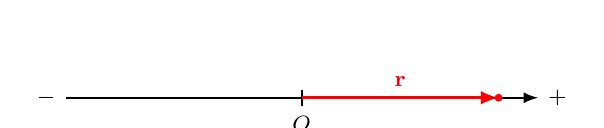
\begin{tikzpicture}
    \draw[axes] (-3,0)--(3,0) node[pos=0,left]{$-$} node[right]{$+$};
    %\foreach \x in {-5,...,5} \draw (\x,.1)--(\x,-.1);
    \draw[thick] (0,.1)--(0,-.1) node[below]{$O$};
    \fill[red] (2.5,0) circle (.05);% node[below]{$A$};
    \draw[vectors,red] (0,0)--(2.5,0) node[midway,above]{$\mathbf r$};
  \end{tikzpicture}
  \caption{Position in a one-dimensional coordinate system}
  \label{fig:1d-position}
\end{figure}

In a two-dimesional coordinate system (e.g.\ $xy$-plane),
%\textbf{Position in 2D Coordinate System:} For two-dimensional motion,
there are several ways to describe an object's position. One way is to use the
$x$ and $y$ coordinates. The positions of the object at $P$ and $Q$ are:
\begin{align*}
  \vec r_P & =3\hat x + 2\hat y\\
  \vec r_Q & =-4\hat x + 3\hat y
\end{align*}
or the length of the straight line from the origin to
the position, and the angle it makes with the $x$ axis.
\begin{figure}[ht]
  \centering
  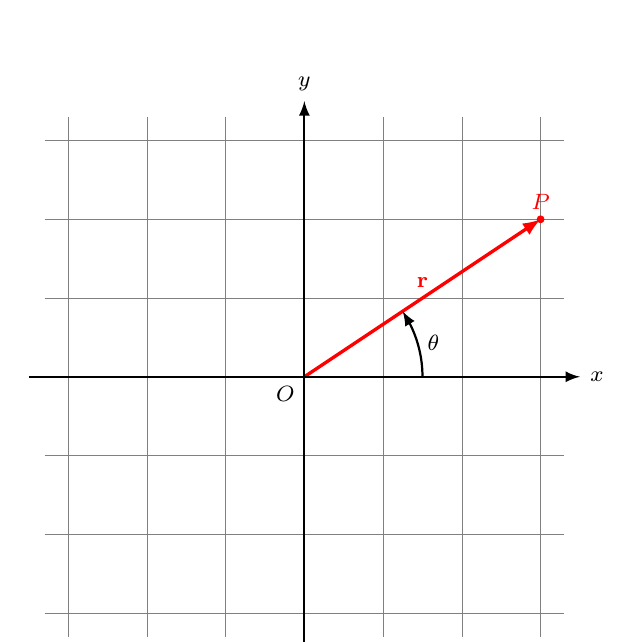
\begin{tikzpicture}
    \draw[help lines] (-3.3,-3.3) grid (3.3,3.3);
    \fill[red] (3,2) circle (.05) node[above]{$P$};
    \draw[vectors,red] (0,0)--(3,2) node[midway,above]{$\mathbf r$};
    \draw[axes] (-3.5,0)--(3.5,0) node[right]{$x$};
    \draw[axes] (0,-3.5)--(0,3.5) node[above]{$y$};
    \draw[axes] (1.5,0) arc (0:atan(2/3):1.5) node[midway,right]{$\theta$};
    \node[below left] at (0,0) {$O$};
  \end{tikzpicture}
  \caption{Position in a two-dimensional coordinate system}
\end{figure}



\subsection{Displacement}
\textbf{Displacement} ($\Delta\mathbf r$) is the \emph{change in position} when
an object moves through the coordinate system. Mathematically, displacement is
defined as the \emph{difference} between the initial position
$\mathbf r_1=\mathbf r(t_1)$ when motion begins, and the current position
$\mathbf r(t)$ of the object. Therefore, as the object moves, $\Delta\mathbf r$
is also a continuous function of time, i.e.:
%\begin{equation*}
%  \Delta\mathbf r=  \Delta\mathbf r(t)
%\end{equation*}
\begin{equation}
  \boxed{
    \Delta\mathbf r(t)=\mathbf r(t)-\mathbf r_1
  }
\end{equation}
Graphically, displacement is drawn as a vector pointing from the initial
position $\mathbf r_1$ towards the current/final position $\mathbf r$.
%\begin{figure}[ht]
%  \centering
%  \begin{tikzpicture}[scale=.5]
%    \draw[axes] (0,0)--(6,0) node[right]{$x$};
%    \draw[axes] (0,0)--(0,8) node[above]{$y$};
%    \draw[vectors,red] (0,0)--(4,1) node[midway,above]{$\mathbf r_1$};
%    \draw[vectors,red] (0,0)--(2,6) node[midway,left]{$\mathbf r_2$};
%    \draw[vectors,blue] (4,1)--(2,6) node[midway,right]{$\Delta\mathbf r$};
%  \end{tikzpicture}
%\end{figure}

\begin{figure}[ht]
  \centering
  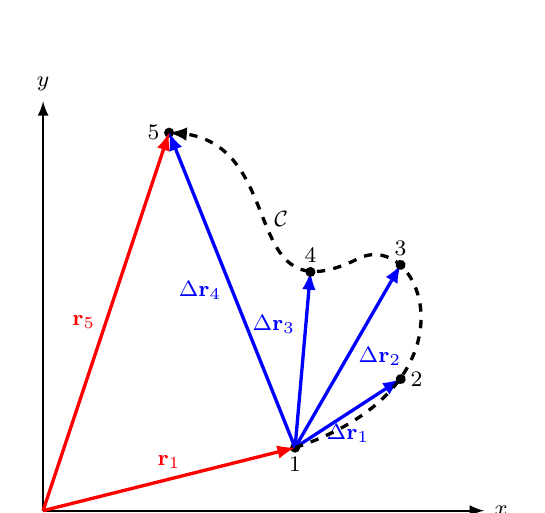
\begin{tikzpicture}[scale=.8]
    \draw[axes] (0,0)--(7,0) node[right]{$x$};
    \draw[axes] (0,0)--(0,6.5) node[above]{$y$};
    \fill (4,1) circle (.08) node[below]{1};
    \fill (2,6) circle (.08) node[left]{5};
    \draw[vectors,red] (0,0)--(4,1) node[midway,above]{$\mathbf r_1$};
    \draw[vectors,red] (0,0)--(2,6) node[midway,left] {$\mathbf r_5$};
    \begin{scope}[rotate around={33:(4,1)}]
      \draw[vector,blue] (4,1)--+(2,0) node[midway,below]{$\Delta\mathbf r_1$};
      \fill (6,1) circle (.08) node[right]{2};
    \end{scope}
    \begin{scope}[rotate around={60:(4,1)}]
      \draw[vector,blue] (4,1)--+(3.35,0) node[midway,right]{$\Delta\mathbf r_2$};
      \fill (7.35,1) circle (.08) node[above]{3};
    \end{scope}
    \begin{scope}[rotate around={85:(4,1)}]
      \draw[vector,blue] (4,1)--+(2.8,0) node[pos=.7,left=0]{$\Delta\mathbf r_3$};
      \fill (6.8,1) circle (.08) node[above]{4};
    \end{scope}
    \draw[vectors,blue] (4,1)--(2,6) node[midway,left]{$\Delta\mathbf r_4$};
    %\fill (7,2) circle (.07);
    %\fill (6,4.5) circle (.07);
    %\fill[cyan] (3,3) circle (.07);
    %\fill[cyan] (4,6) circle (.07);
    \draw[very thick,dashed,->] (4,1) ..controls (7,2) and (6,4.5).. (5,4)
    ..controls (3,3) and (4,6).. (2,6) node[midway,right]{$\mathcal C$};
  \end{tikzpicture}
  \caption{The displacement of an object evolves with time as it moves.}
\end{figure}


The SI unit for displacement is also \textbf{metre} (\si\metre).



\textbf{Explain why this is a subtraction}


\subsection{Distance}

\textbf{Distance} ($s$) is a quantity that is \emph{similar} to
displacement. It is the length of the path $\mathcal C$ taken as an object
moves from initial position ($\mathbf r_1$) to its current/final position
($\mathbf r(t)$). Unlike displacement, distance is a \emph{length}, and therefore
it is \emph{scalar} quantity. For the same reason, distance is non-negative
(i.e.\ $s\geq 0$). As the object moves, distance is always increasing. Since
the length changes with time, distance is also a continuous function of time:
\begin{equation*}
  \boxed{s=s(t)}
\end{equation*}
%\item Depends on \emph{how} the object travels from $\mathbf r_1$ to
%  $\mathbf r_2$
Although the magnitude of the displacement vector $|\Delta\mathbf r|$ is also a
scalar, it is \emph{not} necessarily the same as distance. In classical
physics,  $s\geq |\Delta\mathbf r|$

%\begin{figure}
%  \centering
%  \begin{tikzpicture}[scale=.5]
%    \draw[axes] (0,0)--(6,0) node[right]{$x$};
%    \draw[axes] (0,0)--(0,8) node[above]{$y$};
%    \draw[vectors,red] (0,0)--(4,1) node[midway,above]{$\mathbf r_1$};
%    \draw[vectors,red] (0,0)--(2,6) node[midway,left] {$\mathbf r_2$};
%    \draw[vectors,blue] (4,1)--(2,6) node[midway,right]{$\Delta\mathbf r$};
%    \draw[very thick,dash dot] (4,1)..controls (6,5) and (5,7)..(2,6)
%    node[midway,right]{$s$};
%  \end{tikzpicture}
%\end{figure}




\subsection{Velocity}

\textbf{Average velocity} ($\mathbf v_\text{avg}$) is how quickly your position
changes \emph{over a finite time interval}. It is a vector quantity with an
SI unit of \textbf{metres per second} (\si{\metre\per\second}). The direction
of $\mathbf v_\text{avg}$ is the same as displacement $\Delta\mathbf d$, and it is
also a function of time:
\begin{equation}
  \boxed{
    \mathbf v_\text{avg}(t)
    =\frac{\Delta\mathbf r(t)}{\Delta t}
    =\frac{\mathbf r(t)-\mathbf r_1}{t-t_1}
  }
\end{equation}
where $\mathbf r_1=\mathbf r(t_1)$ is the initial position at initial time $t_1$

In contrast, \textbf{instantaneous velocity} ($\mathbf v$) is how quickly
your displacement is changing \emph{at a specific instance in time}
\begin{itemize}
\item Obtained by letting the time interval \emph{infinitesimally} small,
  i.e.\ $\Delta t\rightarrow 0$
\item Also called the \emph{rate of change in displacement}
\item Calculating instantaneous velocity may require calculus\footnote{For
those of you who know a bit of calculus, the definition of instantenous
velocity is:
\begin{displaymath}
  \mathbf v(t)=\frac{d\mathbf r}{dt}
\end{displaymath}}  
\end{itemize}




\subsection{Speed}

\textbf{Average speed} ($v$) is similar to average velocity, but instead of
using displacement, it is the distance ($s$) travelled over a \emph{finite}
time interval. Speed is a \emph{scalar}:
  
\begin{equation}
  \boxed{
    v_\text{avg}(t)
    =\frac{s(t)}{\Delta t}\geq 0
  }
\end{equation}
Similarly, \textbf{instantaneous speed} ($v$) is how quickly
distance is changing at a \emph{specific instance} in time.
\begin{itemize}
\item Since distance is always positive ($s\ge 0$), both average and
  instantaneous speeds must always be positive
\end{itemize}




\subsection{Acceleration}

\textbf{Average acceleration} ($\mathbf a_\text{avg}$) is how quickly the
instantaneous velocity vector changes over a \emph{finite} time interval,
with an SI unit of \textbf{metres per second squared}
(\si{\metre\per\second\squared}):
\begin{equation}
  \boxed{\mathbf a_\text{avg}(t)
    =\frac{\Delta\mathbf v(t)}{\Delta t}
    =\frac{\mathbf v(t)-\mathbf v_1}{t-t_1}
  }
\end{equation}
where $\mathbf v_1=\mathbf v(t_1)$ is the initial velocity $\mathbf v$ at initial time
$t_1$.

\textbf{Instantaneous acceleration} ($\mathbf a(t)$) is how quickly the velocity
vector is changing at a \emph{specific instance} in time

A few things to note about acceleration:
\begin{itemize}
\item i.e.\ \emph{the rate of change of instantaneous velocity}
\item A change in a vector ($\Delta\mathbf v$) can mean a change in magnitude
  and/or direction
\item There can be acceleration without any speeding up or slowing down!
\item Think  about what happens if a car is turning at constant speed
\end{itemize}




%\section{Working with Vectors}
%  Vectors obey the \emph{principle of superposition}, which means that they
%  \emph{add} together. Methods for adding vectors include:
%  \begin{itemize}
%  \item Using \textbf{Pythagorean theorem} (for vectors at right angles to
%    each other)
%  \item Using \textbf{cosine and sine laws}
%  \item Decomposing vectors into \textbf{components}, then reassemble them
%    using Pythagorean theorem
%  \end{itemize}
%  For 1D problems, ($+$) and ($-$) signs are sufficient to indicate direction
%  \begin{itemize}
%  \item Remember to indicate which way is positive though!
%  \end{itemize}
%  \textbf{WARNING:} When adding vectors, you
%  \underline{\textbf{\emph{must not}}} simply add the magnitudes of the vectors!



%
%\section{Basic Motion Graphs}
%We can describe \emph{one-dimensional} motion graphically using
%\textbf{motion graphs}, by plotting
%\begin{itemize}
%\item Position vs.\ time ($d$--$t$)
%\item Instantaneous velocity vs.\ time ($v$--$t$)
%\item Instantaneous acceleration vs.\ time ($a$--$t$)
%\end{itemize}



\section{Basic Motion Graphs}
In one-dimension, motion can 
%  %the kinematic equations\footnote{They can only
%  %  be used for constant acceleration!} can
also be expressed graphically using \textbf{motion graphs}. The most basic
motion graphs are motion quantities as functions of time:
\begin{itemize}[itemsep=3pt]
\item Position vs.\ time ($r$ vs.\ $t$)
\item Instantaneous velocity vs.\ time ($v$ vs.\ $t$)
\item Instantaneous acceleration vs.\ time ($a$ vs.\ $t$)
\end{itemize}
At the moment, we are interested in:
\begin{itemize}[itemsep=3pt]
\item What the graphs themselves tell us
\item What the slopes of the graphs tell us
\item What the areas under the graphs tell us
\end{itemize}



\subsection{Position vs.\ Time Graph}
The \emph{most} obvious choice for expressing 1D motion of an object
graphically is by plotting its position as a function of time ($r(t)$). An
example is shown in Fig.~\ref{fig:pos-time-graph}.
\begin{figure}[ht]
  \centering
  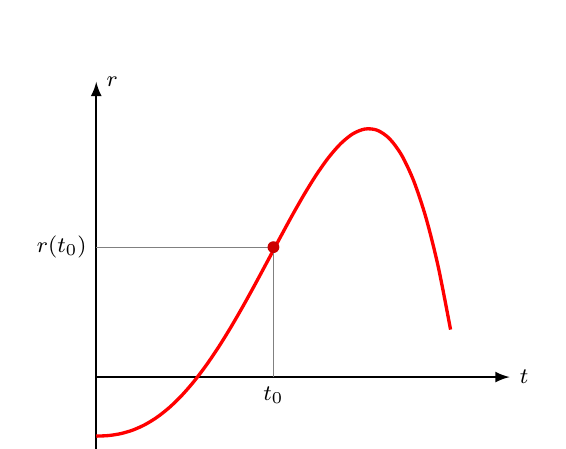
\begin{tikzpicture}[scale=1.5]
    \draw[axes] (0,0)--(3.5,0) node[right]{$t$};
    \draw[axes] (0,-.7)--(0,2.5) node[right]{$r$};
    \draw[functions,smooth,samples=30,domain=0:3]
    plot({\x},{-.2*\x^4+.5*\x^3+.4*\x^2-.5});
    
    \draw[gray] (1.5,0)--(1.5,1.1) node[pos=0,below,black]{$t_0$}
    --(0,1.1) node[left,black]{$r(t_0)$};
    \fill[red!80!black] (1.5,1.1) circle (.05);
  \end{tikzpicture}
  \caption{A typical position vs.\ time graph}
  \label{fig:pos-time-graph}
\end{figure}   
In a position vs.\ time graph, the horizontal ($x$) axis (independent variable)
is time $t$, while the the vertical ($y$) axis (dependent variable) is the
position $r$ measured from origin.
%\item Position in one-dimension can be $+/-$
%Generally, motion begins at $t=0$.
As shown in Figure~\ref{fig:pos-time-graph}, to find position at time $t_0$,
you can simply read the graph!
%\item Time only moves forward, but the graph does not explicitly tell you
%  so




\subsubsection{Slope of Secant: Average Velocity}
\textbf{Average velocity} of an object's motion is the
\emph{slope of the secant} of the position vs.\ time graph.
\begin{figure}[ht]
  \centering
  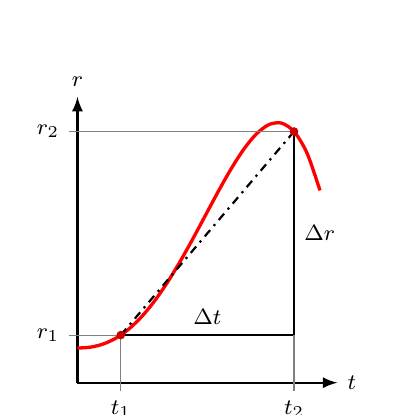
\begin{tikzpicture}[scale=1.1]
    \draw[axes] (0,0)--(0,3.3) node[above]{$r$};
    \draw[axes] (0,0)--(3,0) node[right]{$t$};
    \draw[functions,smooth,samples=20,domain=0:2.8]
    plot({\x},{-.2*\x^4+.5*\x^3+.4*\x^2+.4});
    \draw[thick,dash dot](.5,.55)--(2.5,2.9);
    \draw[thick] (.5,.55)--(2.5,.55)node[midway,above]{$\Delta t$}
    --(2.5,2.9) node[midway,right]{$\Delta r$};
    \draw[gray] (.5,.55)--(.5,-.1) node[below,black]{$t_1$};
    \draw[gray] (2.5,.55)--(2.5,-.1) node[below,black]{$t_2$};
    \draw[gray] (.5,.55)--(-.1,.55) node[left,black]{$r_1$};
    \draw[gray] (2.5,2.9)--(-.1,2.9) node[left,black]{$r_2$};
    \fill[red!80!black] (.5,.55) circle (.05);
    \fill[red!80!black] (2.5,2.9) circle (.05);
  \end{tikzpicture}
  \hspace{.1in}
  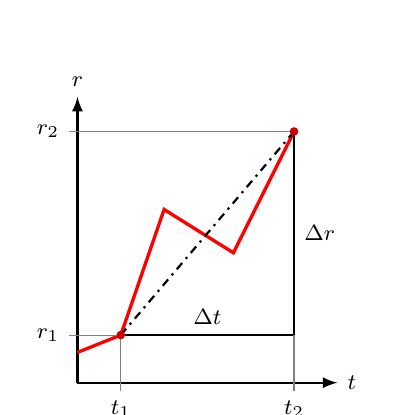
\begin{tikzpicture}[scale=1.1]
    \draw[axes] (0,0)--(0,3.3) node[above]{$r$};
    \draw[axes] (0,0)--(3,0) node[right]{$t$};
    \draw[functions] (0,.35)--(.5,.55)--(1,2)--(1.8,1.5)--(2.5,2.9);
    \draw[thick,dash dot] (.5,.55)--(2.5,2.9);
    \draw[thick] (.5,.55)--(2.5,.55)node[midway,above]{$\Delta t$}
    --(2.5,2.9) node[midway,right]{$\Delta r$};
    \draw[gray] (.5,.55)--(.5,-.1) node[below,black]{$t_1$};
    \draw[gray] (2.5,.55)--(2.5,-.1) node[below,black]{$t_2$};
    \draw[gray] (.5,.55)--(-.1,.55) node[left,black]{$r_1$};
    \draw[gray] (2.5,2.9)--(-.1,2.9) node[left,black]{$r_2$};
    \fill[red!80!black] (.5,.55) circle (.05);
    \fill[red!80!black] (2.5,2.9) circle (.05);
    \end{tikzpicture}
\end{figure}
%  \vspace{-.1in}Same average velocity in both graphs, but very different
%  motions
%  \begin{itemize}
%  \item ($+$) slope: motion in the ($+$) direction during the time interval
%  \item ($-$) slope: motion in the ($-$) direction during the time interval
%  \item Zero slope: no displacement over this time interval
%  \end{itemize}
%\end{frame}
%
%
%
\subsubsection{Instantaneous Velocity:} The instantaneous velocity of an object
is the \emph{slope of the tangent} to the curve of the position vs.\ time graph
at a specific time.
\begin{figure}[ht]
  \centering
  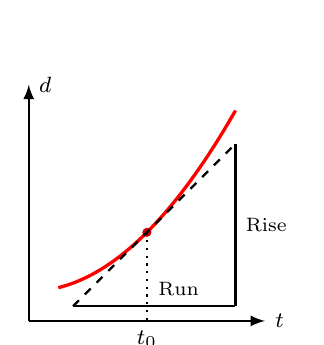
\begin{tikzpicture}[scale=.75]
    \draw[axes] (0,0)--(4,0) node[right] {$t$};
    \draw[axes] (0,0)--(0,4) node[right] {$d$};
    \draw[functions,smooth,samples=20,domain=.5:3.5]
    plot({\x},{.25*\x^2+.5});
    \fill[red!80!black] (2,1.5) circle (2.2pt);
    \draw[dotted,thick] (2,1.5)--(2,0) node[below] {$t_0$};
    
    \draw[smooth,samples=4,domain=.75:3.5,thick,dashed]
    plot({\x},{\x-.5});
    \draw[thick] (.75,.25)--(3.5,.25) node[pos=.65,above] {\scriptsize Run};
    \draw[thick] (3.5,.25)--(3.5,3) node[midway,right] {\scriptsize Rise};
    
  \end{tikzpicture}
\end{figure}

Like average velocity, the sign of the slope also indicates the direction of
motion. If position data is obtained experimentally, it may be difficult to
obtain an accurate value for instantaneous velocity.

%  What can we learn about instantaneous velocity from this position vs.\ time
%  graph?
%\begin{figure}
%  \begin{center}
%    \begin{tikzpicture}
%      \draw[axes] (0,0)--(3.5,0) node[right]{$t$};
%      \draw[axes] (0,-.7)--(0,2.5) node[right]{$d$};
%      \draw[functions,smooth,samples=30,domain=0:3]
%      plot({\x},{-.2*\x^4+.5*\x^3+.4*\x^2-.5});
%      \uncover<2->{
%        \begin{scope}[thick,cyan]
%          \draw (-.4,-.5)--+(.8,0) node[midway,below=-2]{$v=0$};
%          \draw (1.9,2.1)--+(.8,0) node[midway,above=-2]{$v=0$};
%          \draw (2.3,2.1)--(2.3,0) node[below=-2]{$t_1$};
%          \draw (0,-.5)--(0,0);
%        \end{scope}
%        \fill[cyan] (0,-.5) circle (.07);
%        \fill[cyan] (2.3,2.1) circle (.07);
%      %  \draw[dash dot,thick] (1.5,0)--(1.5,1.1) node[pos=0,below]{$t_0$}
%      %  --(0,1.1) node[left]{$d(t_0)$};
%      %  \fill[red!80!black] (1.5,1.1) circle (.05);
%      }
%      \uncover<3->{
%        \fill[pink!35,opacity=.3] (0,-.7) rectangle (2.3,2.3);
%        \draw[<-,thick,red] (.75,1) to[out=120,in=0] +(-1,.2)
%        node[left,text width=98,draw=red,fill=magenta!10]{\scriptsize
%          For $0<t<t_0$, velocity is positive ($v>0$) because the graph has a
%          positive slope\par};
%      }
%      \uncover<4->{
%        \fill[cyan!35,opacity=.3] (2.3,-.7) rectangle (3,2.3);
%        \draw[<-,thick,blue] (2.6,1) to[out=90,in=180] +(1.6,.4)
%        node[right,text width=86,draw=blue,fill=cyan!30]{\scriptsize
%          For $t>t_0$, velocity is negative ($v<0$) because the slope is
%          negative\par};
%      }
%    \end{tikzpicture}
%  \end{center}
%\end{frame}
%
%
%
%
\textbf{Acceleration:} Finding instantaneous acceleration $a(t)$ from a
position vs.\ time graph is \emph{very} difficult\footnote{If you already know
the function $r(t)$ exactly, then you can use calculus to find acceleration
exactly. In that case you don't really \emph{need} this graph in the first
place.}, but we can still find the \emph{sign} of acceleration based on whether
the graph opens up or down.
%In this example:
\begin{figure}[ht]
  \centering
  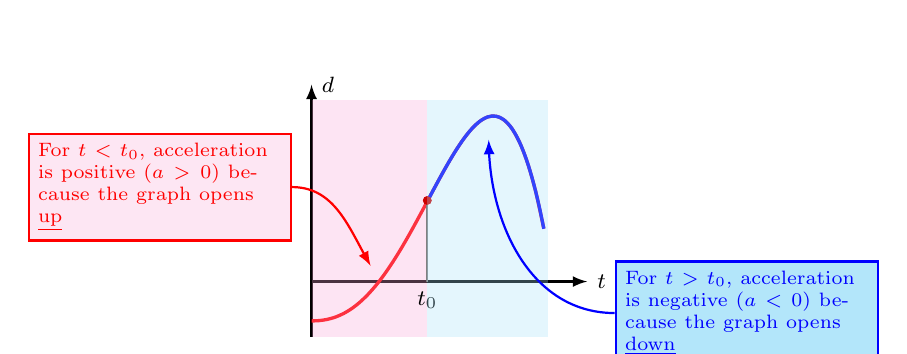
\begin{tikzpicture}
    \draw[axes] (0,0)--(3.5,0) node[right]{$t$};
    \draw[axes] (0,-.7)--(0,2.5) node[right]{$d$};
    \draw[functions,smooth,samples=30,domain=0:2.95]
    plot({\x},{-.2*\x^4+.5*\x^3+.4*\x^2-.5});
    %\uncover<2->{
      \fill[magenta!35,opacity=.3] (0,-.7) rectangle (1.47,2.3);
      \draw[<-,thick,red] (.75,.2) to[out=120,in=0] +(-1,1)
      node[left,text width=88,draw=red,fill=magenta!10]{\scriptsize
        For $t<t_0$, acceleration is positive ($a>0$) because the graph opens
        \underline{up}\par};
      \draw[thick,gray](1.47,1.03)--(1.47,0) node[below,black]{$t_0$};
      \fill[red!80!black] (1.47,1.03) circle (.055);
    %}
    %\uncover<3->{
      \draw[functions,smooth,samples=30,domain=1.48:2.95,blue]
      plot({\x},{-.2*\x^4+.5*\x^3+.4*\x^2-.5});
      \fill[red!80!black] (1.47,1.03) circle (.055);
      \fill[cyan!35,opacity=.3] (1.47,-.7) rectangle (3,2.3);
      \draw[<-,thick,blue] (2.25,1.8) to[out=270,in=180] +(1.6,-2.2)
      node[right,text width=88,draw=blue,fill=cyan!30]{\scriptsize
        For $t>t_0$, acceleration is negative ($a<0$) because the graph opens
        \underline{down}\par};
    %}
  \end{tikzpicture}
\end{figure}

%
%
%
\subsection{Velocity vs.\ Time Graph}

A less obvious choice for expressing 1D motion is by plotting
\emph{instantaneous} velocity as a function of time, i.e.\ $v=v(t)$. In
essence, we are plotting the slope of the position vs.\ time graph instead.
Using our example position vs.\ time graph:

\begin{figure}[ht]
  \centering
  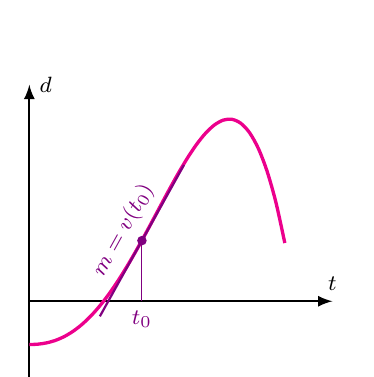
\begin{tikzpicture}[scale=1.1]
    \draw[axes] (0,0)--(3.5,0) node[above]{$t$};
    \draw[axes] (0,-1)--(0,2.5) node[right]{$d$};
    \draw[functions,smooth,samples=30,domain=0:2.95,magenta]
    plot(\x,{-.2*\x^4+.5*\x^3+.4*\x^2-.5});

    \fill[violet] (1.3,.7) circle (.055);
    \draw[violet] (1.3,.7)--(1.3,0) node[below]{$t_0$};
    \draw[thick,violet,rotate around={atan(1.8):(1.3,.7)}] (.3,.7)--+(2,0)
    node[midway,above,rotate=atan(1.8)]{$m=v(t_0)$};
  \end{tikzpicture}
  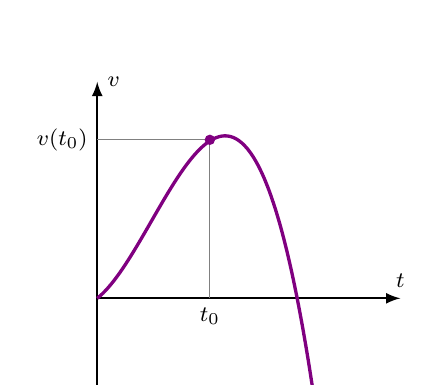
\begin{tikzpicture}[scale=1.1]
    \draw[axes] (0,0)--(3.5,0) node[above]{$t$};
    \draw[axes] (0,-1)--(0,2.5) node[right]{$v$};
    \draw[smooth,samples=40,domain=0:2.5,functions,violet]
    plot(\x,{-.8*\x^3+1.5*\x^2+.8*\x});
    \draw[gray] (1.3,0)--(1.3,1.83) node[pos=0,below,black]{$t_0$}
    --(0,1.83) node[left,black]{$v(t_0)$};
    \fill[violet] (1.3,1.83) circle (.06);
  \end{tikzpicture}

\end{figure}

%
%
%
%\begin{frame}{Velocity vs.\ Time Graph}
%%  \begin{columns}
%%    \column{.7\textwidth}
%%    \begin{itemize}
%  The velocity vs.\ time graph shows how instantaneous velocity evolves with
%  time. In this example:
%%    \item<3->Slope of the secant: average acceleration
%%    \item<3->Slope of the tangent: instantaneous acceleration
%%    \end{itemize}
%%    
%%    \column{.3\textwidth}
%  \begin{center}
%    \begin{tikzpicture}
%      \draw[axes] (0,0)--(3,0) node[right=-2]{$t$};
%      \draw[axes] (0,-1.5)--(0,2.2) node[above=-2]{$v$};
%      \draw[smooth,samples=45,domain=0:2.55,very thick,violet]
%      plot(\x,{-.8*\x^3+1.5*\x^2+.8*\x});
%      \uncover<2->{
%        \fill[violet] (2.3,0) circle (.055) node[below left=-2]{$t_1$};
%        \fill[violet] circle (.055) node[left=-2]{$0$};
%        \draw[<-,violet,thick] (-.4,0)--+(-3,0)
%        node[text width=80,draw=violet,fill=violet!10]{\scriptsize
%          At $t=0$ and $t=t_1$, velocity is zero ($v=0$)\par};
%      }
%      \uncover<3->{
%        \draw[gray] (1.47,1.87)--(1.47,0) node[below,violet]{$t_0$};
%        \fill[violet] (1.47,1.87) circle (.055);
%        \draw[<-,thick,violet] (1.55,1.87) to[out=30,in=150] +(1.6,0)
%        node[right,text width=75,draw=violet,fill=violet!10]{\scriptsize
%          At $t=t_0$, velocity is maximum. The slope is zero at this point.
%          \par};
%      }
%    \end{tikzpicture}
%  \end{center}
%  Velocity is positive when the graph is above the time axis; and negative
%  when below the time axis
%
%%    \begin{tikzpicture}[scale=1.1]
%%      \draw[axes] (0,0)--(3.5,0) node[above]{$t$};
%%      \draw[axes] (0,-1.25)--(0,2.75) node[right]{$v$};
%%      \draw[functions,smooth,samples=40,domain=0:3]
%%      plot({\x},{1.35*(\x-1)*(\x-1)-1.1*\x+.5});
%%      \uncover<2>{
%%        \draw[smooth,samples=40,domain=.626:2.189,orange,very thick]
%%        plot({\x},{1.35*(\x-1)*(\x-1)-1.1*\x+.5});
%%        \draw[smooth,samples=40,domain=2.189:3,violet,very thick]
%%        plot({\x},{1.35*(\x-1)*(\x-1)-1.1*\x+.5});
%%        \draw[smooth,samples=40,domain=0:.626,violet,very thick]
%%        plot({\x},{1.35*(\x-1)*(\x-1)-1.1*\x+.5});
%%      }
%%    \end{tikzpicture}
%%  \end{columns}
%\end{frame}
%
%

\textbf{Average Acceleration:}
%  \begin{center}
%    \begin{tikzpicture}[scale=1.1]
%      \draw[axes] (0,0)--(3,0) node[right=-2]{$t$};
%      \draw[axes] (0,-1.5)--(0,2.2) node[above=-2]{$v$};
%      \draw[smooth,samples=45,domain=0:2.55,very thick,violet]
%      plot(\x,{-.8*\x^3+1.5*\x^2+.8*\x});
%      %\uncover<2->{
%      %  \fill[violet] (2.3,0) circle (.055) node[below left=-2]{$t_1$};
%      %  \fill[violet] (0,0) circle (.055) node[left=-2]{$0$};
%      %}
%    \end{tikzpicture}
%  \end{center}
%\end{frame}
%
%
%
\textbf{Instantaneous Acceleration:}
%  \begin{center}
%    \begin{tikzpicture}[scale=1.1]
%      \draw[axes] (0,0)--(3,0) node[right=-2]{$t$};
%      \draw[axes] (0,-1.5)--(0,2.2) node[above=-2]{$v$};
%      \draw[smooth,samples=45,domain=0:2.55,very thick,violet]
%      plot(\x,{-.8*\x^3+1.5*\x^2+.8*\x});
%      %\uncover<2->{
%      %  \fill[violet] (2.3,0) circle (.055) node[below left=-2]{$t_1$};
%      %  \fill[violet] (0,0) circle (.055) node[left=-2]{$0$};
%      %}
%    \end{tikzpicture}
%  \end{center}



\textbf{Displacement and position:} The area under the velocity vs.\ time graph
is the \emph{displacement} of the object. In example below, the shaded area is
the displacement between $t_1$ and $t_2$. If the position at $t_1$ (i.e.\
$d_1$) is also known, then we can find the position at $t_2$ (i.e.\
$d_2=d_1+\Delta d$).
\begin{figure}[ht]
  \centering
  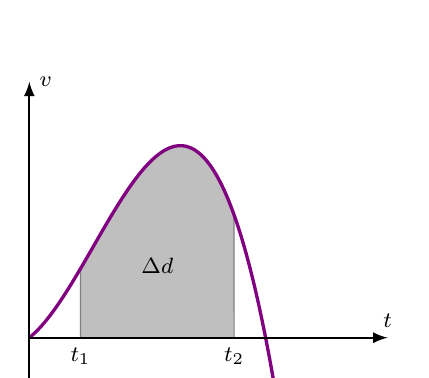
\begin{tikzpicture}[scale=1.3]
    \draw[smooth,samples=30,domain=.5:2,gray,fill=lightgray]
    plot(\x,{-.8*\x^3+1.5*\x^2+.8*\x})--(2,0) node[below,black]{$t_2$}
    --(.5,0) node[below,black]{$t_1$}--cycle;

    \draw[smooth,samples=50,domain=0:2.4,functions,violet]
    plot(\x,{-.8*\x^3+1.5*\x^2+.8*\x});

    \draw[axes] (0,0)--(3.5,0) node[above]{$t$};
    \draw[axes] (0,-.5)--(0,2.5) node[right]{$v$};

    \node at (1.25,.7) {$\Delta d$};
  \end{tikzpicture}
  \caption{The area under the velocity vs.\ time graph between $t_1$ and $t_2$
    gives us the object's displacement during this time interval.}
  \label{fig:area-under-vt-graph}
\end{figure}
If the area is \emph{above} the $x$-axis (time axis), then displacement
is positive ($\Delta d>0$); if the area is \emph{below} the $x$-axis, then
displacement is negative ($\Delta d<0$).



\subsection{Acceleration vs. Time Graph}
In the same way that we convert a position vs.\ time graph to a velocity vs.\
time graph, we can also convert a velocity vs.\ time graph to an
\textbf{acceleration vs.\ time} graph, by plotting the slope of the tangent.
This graph shows how \emph{instantaneous} acceleration $a(t)$ evolves with
time. In the example below:
%    \centering
%    \begin{tikzpicture}[scale=1.1]
%      \draw[axes] (0,0)--(3,0) node[right]{$t$};
%      \draw[axes] (0,-1)--(0,2.5) node[right]{$v$};
%      \draw[smooth,samples=40,domain=0:2.4,functions,violet]
%      plot(\x,{-.8*\x^3+1.5*\x^2+.8*\x});
%      %\fill[violet] (1.3,.7) circle (.06);
%      %\draw[violet] (1.3,.7)--(1.3,0) node[below]{$t_0$};
%    \end{tikzpicture}
%    
%    \column{.3\textwidth}
%    \centering
%    \begin{tikzpicture}[scale=1.1]
%      \draw[axes] (0,0)--(3,0) node[right]{$t$};
%      \draw[axes] (0,-2.3)--(0,1.2) node[right]{$a$};
%      \draw[smooth,samples=40,domain=0:2.2,functions,orange]
%      plot(\x,{-1.2*\x^2+1.5*\x+.4});
%      %\draw[gray] (1.3,0)--(1.3,1.83) node[pos=0,below,black]{$t_0$}
%      %--(0,1.83) node[left,black]{$v(t_0)$};
%      %\fill[violet] (1.3,1.83) circle (.06);
%    \end{tikzpicture}
%  \end{columns}

%\begin{frame}{Acceleration vs.\ Time Graph}

%  \begin{center}
%    \begin{tikzpicture}[scale=1.1]
%      \draw[axes] (0,0)--(2.8,0) node[right=-2]{$t$};
%      \draw[axes] (0,-2)--(0,1.2) node[right=-2]{$a$};
%      \draw[smooth,samples=40,domain=0:2.2,functions,orange]
%      plot(\x,{-1.2*\x^2+1.5*\x+.4});
%      \uncover<2->{
%        \fill[pink!40,opacity=.4] (0,-2) rectangle (1.48,1);
%        \fill[orange] (0.63,.87) circle (.06);
%        \draw[gray] (.63,0)--(.63,.87) node[pos=0,below=-2,black]{$t_0$}
%        --(0,.87) node[left=-2,black]{$a_\text{max}$};
%        \fill[orange] (1.48,0) circle (.06) node[above,black]{$t_1$};
%        \draw[thick,magenta,<-] (.75,-1)--+(-1,0)
%        node[left,text width=80,draw=magenta]{\scriptsize
%          Acceleration is positive from $t=0\rightarrow t_1$, with a maximum
%          magnitude of $a_\text{max}$ at $t_0$\par};
%      }
%      \uncover<3->{
%        \fill[violet] (1.48,0) circle (.06) node[above]{$t_1$};
%        \draw[thick,violet,<-] (1.48,.4) to[out=90,in=180] (3,1)
%        node[right,text width=70,draw=violet,fill=violet!10]{\scriptsize
%          Acceleration is zero ($a=0$) at $t=t_1$\par};
%      }
%      \uncover<4->{
%        \fill[cyan!40,opacity=.4] (1.48,-2) rectangle (2.4,1);
%        \draw[thick,blue,<-] (2.1,-.8)--+(1,0)
%        node[right,text width=63,draw=blue,fill=cyan!10]{\scriptsize
%          Acceleration is negative for $t>t_1$\par};
%      }
%    \end{tikzpicture}
%  \end{center}
%  \uncover<4->{
%    \vspace{-.1in}Remember: Since acceleration is a vector, \emph{positive}
%    acceleration means acceleration \emph{in the positive
%    \underline{direction}}, but it does not necessarily mean the object speeds
%    up
%  }
%\end{frame}
%
%

\subsubsection{Slope of the Acceleration vs.\ Time Graph}
The slope of the acceleration vs.\ time graph is the rate of change of
acceleration, called \textbf{jerk}.\footnote{The slope of the tangent is
called \textbf{instantaneous jerk}, whereas the slope of the secant is the
\textbf{average jerk}.}. This is \emph{not} a topic that is covered in Grade
11 or 12 Physics.
\begin{figure}[ht]
  \centering
  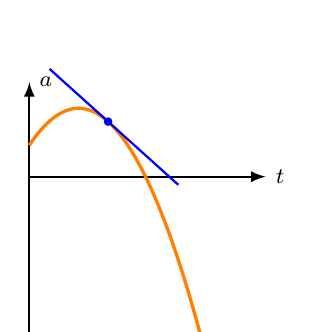
\begin{tikzpicture}
    \draw[axes] (0,0)--(3,0) node[right]{$t$};
    \draw[axes] (0,-2)--(0,1.2) node[right]{$a$};
    \draw[smooth,samples=40,domain=0:2.2,functions,orange]
    plot(\x,{-1.2*\x^2+1.5*\x+.4});
    \fill[blue] (1,.7) circle (.055);
    \draw[blue,thick,rotate around={-atan(.9):(1,.7)}] (0,.7)--+(2.2,0);
  \end{tikzpicture}
\end{figure}



%\begin{frame}{Area Under the Acceleration vs.\ Time Graph}
%  The area under acceleration vs.\ time graph is the \emph{change in velocity}
%  $\Delta v$.
%  \begin{center}
%    \begin{tikzpicture}
%      \draw[axes] (0,0)--(3,0) node[right]{$t$};
%      \draw[axes] (0,-2)--(0,1.2) node[right]{$a$};
%      \draw[smooth,samples=40,domain=0:2.2,functions,orange]
%      plot(\x,{-1.2*\x^2+1.5*\x+.4});
%      \uncover<2->{
%        \draw[smooth,samples=40,domain=.3:1.3,thick,gray,fill=lightgray!50]
%        plot(\x,{-1.2*\x^2+1.5*\x+.4})--(1.3,0) node[below=-2,black]{$t_2$}
%        --(.3,0) node[below=-2,black]{$t_1$}--cycle;
%        \draw[thick,<-,black!80] (.8,.3)--+(-1.5,0)
%        node[text width=72,left,draw=black!80,fill=lightgray!50]{\scriptsize
%          $\Delta v>0$ from $t_1\rightarrow t_2$ because the area is above the
%          $x$ axis\par};
%      }
%      \uncover<3->{
%        \draw[smooth,samples=40,domain=1.7:2.1,thick,cyan,fill=cyan!20]
%        plot(\x,{-1.2*\x^2+1.5*\x+.4})--(2.1,0) node[above=-2]{$t_4$}
%        --(1.7,0) node[above=-2]{$t_3$}--cycle;
%        \draw[thick,<-,blue] (1.9,-.5)--+(2,0)
%        node[text width=75,right,draw=blue,fill=cyan!20]{\scriptsize
%          $\Delta v<0$ from $t_3\rightarrow t_4$ because the area is below the
%          $x$ axis\par};
%      }
%    \end{tikzpicture}
%  \end{center}
%  \begin{itemize}
%  \item If the area is \emph{above} the $x$-axis (time axis), then $\Delta v>0$
%  \item If the area is \emph{below} the $x$-axis, then $\Delta v<0$
%  \item Remember: $\Delta v>0$ does not necessarily mean that the object
%    speeds up; $\Delta v<0$ does not necessarily mean that it will slow down
%  \end{itemize}
%\end{frame}


\section{Uniform Motion}
\textbf{Uniform motion} is when the velocity vector is constant, and neither
its magnitude nor direction changes. In 1D, the motion graphs look like this:
\vspace{-.1in}\begin{center}
  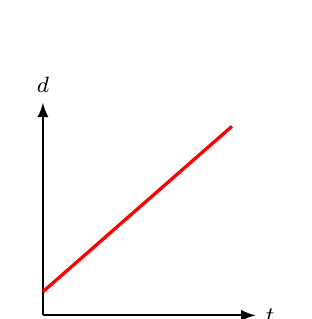
\begin{tikzpicture}[scale=.6]
    \draw[axes] (0,0)--(4.5,0) node[right]{$t$};
    \draw[axes] (0,0)--(0,4.5) node[above]{$d$};
    \draw[functions] (0,.5)--(4,4);
  \end{tikzpicture}
  \hspace{.15in}
  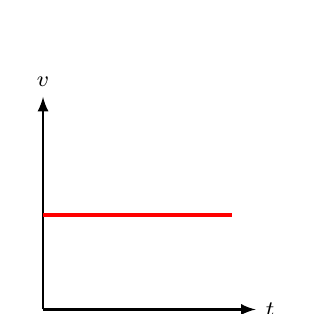
\begin{tikzpicture}[scale=.6]
    \draw[axes] (0,0)--(4.5,0) node[right]{$t$};
    \draw[axes] (0,0)--(0,4.5) node[above]{$v$};
    \draw[functions] (0,2)--(4,2);
  \end{tikzpicture}
  \hspace{.15in}
  \begin{tikzpicture}[scale=.6]
    \draw[axes] (0,0)--(4.5,0) node[right]{$t$};
    \draw[axes] (0,0)--(0,4.5) node[above]{$a$};
    \draw[functions] (0,0)--(4,0);
  \end{tikzpicture}
\end{center}
\begin{itemize}
\item \vspace{-.15in}$d$--$t$ graph is a straight line
\item The slope of the $d$--$t$ graph, which is velocity $v$, is also constant
\item There is no acceleration, so $a=0$ for all $t$
\end{itemize}




\section{Uniform Acceleration}
When a constant net force acts on an object, it moves with a constant
non-zero acceleration, or \textbf{uniform acceleration}.
\begin{center}
  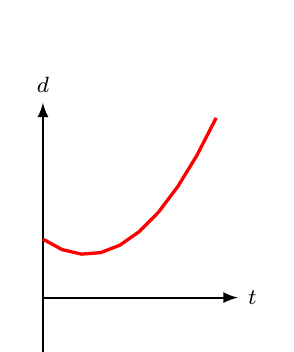
\begin{tikzpicture}[scale=.55]
    \draw[axes] (0,0)--(4.5,0) node[right]{$t$};
    \draw[axes] (0,-1.5)--(0,4.5) node[above]{$d$};
    \draw[functions,samples=10,domain=0:4] plot(\x,{.35*(\x-1)*(\x-1)+1});
  \end{tikzpicture}
  \hspace{.15in}
  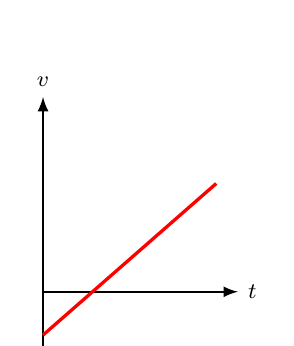
\begin{tikzpicture}[scale=.55]
    \draw[axes] (0,0)--(4.5,0) node[right]{$t$};
    \draw[axes] (0,-1.5)--(0,4.5) node[above]{$v$};
    \draw[functions] (0,-1)--(4,2.5);
  \end{tikzpicture}
  \hspace{.15in}
  \begin{tikzpicture}[scale=.55]
    \draw[axes] (0,0)--(4.5,0) node[right]{$t$};
    \draw[axes] (0,-1.5)--(0,4.5) node[above]{$a$};
    \draw[functions] (0,1)--(4,1);
  \end{tikzpicture}
\end{center}
\begin{itemize}
\item The $d$ vs.\ $t$ graph is part of a \emph{parabola}
  \begin{itemize}
  \item opens \emph{up}, then acceleration is positive
  \item opens \emph{down}, then acceleration is negative
  \end{itemize}
\item The $v$ vs.\ $t$ graph is a straight line; the (constant) slope is the
  cceleration
\end{itemize}




\section{Area Under Motion Graphs}
\begin{center}
  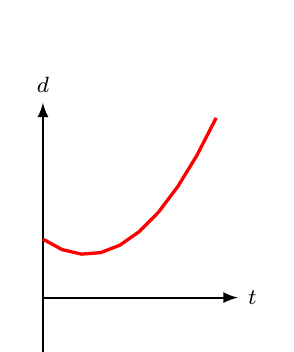
\begin{tikzpicture}[scale=.55]
    \draw[axes] (0,0)--(4.5,0) node[right]{$t$};
    \draw[axes] (0,-1.5)--(0,4.5) node[above]{$d$};
    \draw[functions,samples=10,domain=0:4] plot(\x,{.35*(\x-1)*(\x-1)+1});
  \end{tikzpicture}
  \hspace{.15in}
  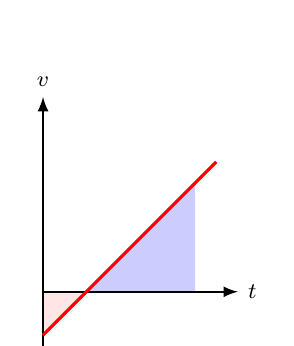
\begin{tikzpicture}[scale=.55]
    \draw[pink!40,fill=pink!40] (0,0)--(0,-1)--(1,0)--cycle;
    \draw[blue!20,fill=blue!20] (1,0)--(3.5,0)--(3.5,2.5)--cycle;
    \draw[axes] (0,0)--(4.5,0) node[right]{$t$};
    \draw[axes] (0,-1.5)--(0,4.5) node[above]{$v$};
    \draw[functions] (0,-1)--(4,3);
  \end{tikzpicture}
  \hspace{.15in}
  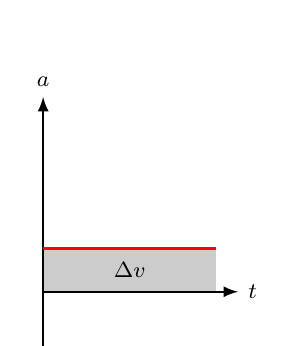
\begin{tikzpicture}[scale=.55]
    \fill[gray!40] rectangle (4,1) node[black,midway]{$\Delta v$};
    \draw[axes] (0,0)--(4.5,0) node[right]{$t$};
    \draw[axes] (0,-1.5)--(0,4.5) node[above]{$a$};
    \draw[functions] (0,1)--(4,1);
  \end{tikzpicture}
\end{center}
\begin{itemize}
\item The area under the $a$--$t$ graph is the change in velocity $\Delta v$
  \begin{itemize}
  \item If initial velocity is known, then we can plot $v$--$t$ graph based on
    this graph
  \end{itemize}
\item The area under the $v$--$t$ graph is the displacement $\Delta d$
  \begin{itemize}
  \item If the area is {\color{red!40}below} the $x$-axis (time axis), then
    displacement is negative;
  \item If the area is {\color{blue!20}above} the time axis, then
    displacement is positive
  \end{itemize}
\item The area under the $d$--$t$ graph has no physical meaning
\end{itemize}




\section{Simple Harmonic Motion}
In \textbf{simple harmonic motion}\footnote{Or \textbf{oscillatory motion},
or \textbf{vibration}}, displacement, velocity and acceleration are all
periodic functions, and none of them are constant!
\vspace{-.1in}
\begin{center}
  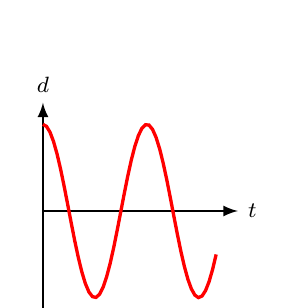
\begin{tikzpicture}[scale=.55]
    \draw[axes] (0,0)--(4.5,0) node[right]{$t$};
    \draw[axes] (0,-2.5)--(0,2.5) node[above]{$d$};
    \draw[functions,samples=50,domain=0:4] plot(\x,{2*cos(150*\x)});
  \end{tikzpicture}
  \hspace{.15in}
  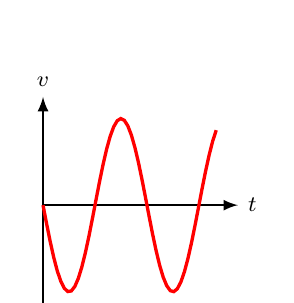
\begin{tikzpicture}[scale=.55]
    \draw[axes] (0,0)--(4.5,0) node[right]{$t$};
    \draw[axes] (0,-2.5)--(0,2.5) node[above]{$v$};
    \draw[functions,samples=50,domain=0:4] plot(\x,{-2*sin(150*\x)});
  \end{tikzpicture}
  \hspace{.15in}
  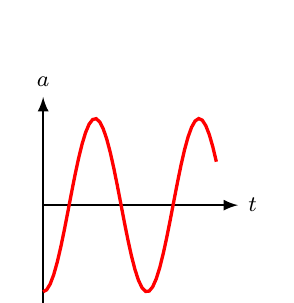
\begin{tikzpicture}[scale=.55]
    \draw[axes] (0,0)--(4.5,0) node[right]{$t$};
    \draw[axes] (0,-2.5)--(0,2.5) node[above]{$a$};
    \draw[functions,samples=50,domain=0:4] plot(\x,{-2*cos(150*\x)});
  \end{tikzpicture}
\end{center}
We will discuss this topic later, in the next unit.



%\section{Example Problem}
%  \textbf{Example:} Expression the motion in a \emph{position-time}
%  graph and an \emph{acceleration-time} graph. Assume the object's initial
%  position is the origin of the coordinate system.
%  \begin{center}
%    \begin{tikzpicture}[scale=.75]
%      \draw[help lines] grid (12,4);
%      \draw[axes] (0,0)--(13,0) node[right]{$t$ (\si\second)};
%      \foreach \t in {0,...,12} {
%        \draw(\t,0)--(\t,-.15) node[below]{$\t$};
%      }
%      \draw[axes] (0,0)--(0,5) node[above]{$v$ (\si{\metre\per\second})};
%      \foreach \v in {0,...,4} {
%        \draw(0,\v,0)--(-.15,\v) node[left]{$\v$};
%      }
%      \draw[functions] (0,2)--(2.5,2)--(5,4)--(7.5,4)--(10,1)--(12,1);
%    \end{tikzpicture}
%  \end{center}
%
%
%
%
\section{1D Kinematic Equations}

\begin{align*}
  \Delta d &=v_1\Delta t + \frac12a\Delta t^2\\
  \Delta d &=v_2\Delta t - \frac12a\Delta t^2\\
  \Delta d &=\frac{v_1+v_2}2 \Delta t\\
  v_2 &= v_1+ a \Delta t\\
  v_2^2 &= v_1^2+ 2a \Delta d
\end{align*}

There are five motion quantities of interest:
\begin{center}
  \begin{tabular}{l|c|c}
    \rowcolor{pink}
    \textbf{Quantity} & \textbf{Symbol} & \textbf{SI Unit} \\ \hline
    Displacement & $\Delta d$ & \si{\metre} \\
    Initial (instantaneous) velocity & $v_1$ & \si{\metre\per\second} \\
    Final (instantaneous) velocity   & $v_2$ & \si{\metre\per\second} \\
    Acceleration (constant) & $a$    & \si{\metre\per\second\squared}\\
    Time interval & $\Delta t$ & \si\second
  \end{tabular}
\end{center}
Only valid for \underline{\textbf{constant acceleration}}



%\section{1D Kinematic Equations}
%  \begin{columns}
%    \column{.35\textwidth}
%    {\large
%      \begin{align*}
%        \Delta d &=v_1\Delta t + \frac12a\Delta t^2\\
%        \Delta d &=v_2\Delta t - \frac12a\Delta t^2\\
%        \Delta d &=\frac{v_1+v_2}2 \Delta t\\
%        v_2 &= v_1+ a \Delta t\\
%        v_2^2 &= v_1^2+ 2a \Delta d
%      \end{align*}
%    }
%    \column{.65\textwidth}
\begin{itemize}
\item For 1-object problems, you are usually given 3 of the 5 variables,
  and you are asked to find a 4th one
\item For 2-object problems, the motion of the two objects are connected by
  time interval $\Delta t$ and displacement $\Delta d$
\item For 2D or 3D problems, each direction should have its own kinematic
  equations
\end{itemize}



%\section{1D Kinematic Equations}
Kinematic equations \emph{cannot} be used when acceleration is non-uniform
(when non-constant forces act on an object):
\begin{itemize}
\item Aerodynamic forces
  \begin{itemize}
  \item Lift and drag forces
  \item proportional to $v^2$
  \end{itemize}
\item Spring force
  \begin{itemize}
  \item The force that a compressed/stretched spring applies to connected
    objects
  \item Proportional to spring displacement $\mathbf x$
  \end{itemize}
\item Dampers in springs
  \begin{itemize}
  \item Dampers are used to slow down the vibration of an object
  \item Generally proportional to $v$
  \end{itemize}
\end{itemize}  
%We will discuss more about forces later in this unit.




%\section{Relative Motion}
%  \begin{center}
%    \vspace{-.15in}
%    \pic{.65}{graphics/57}
%  \end{center}
%  \begin{itemize}
%  \item Observers (frames of reference) A and B measures different motion of the
%    ball because A and B a moving relative to each other
%  \item The instantaneous velocity of the ball at any time $t$, as measured by
%    A and B, is related by the instantaneous velocities of A and B relative to
%    each other
%  \end{itemize}
%
%
%
%
%\section{Relative Motion}
%  All velocities are measured \emph{relative} to a frame of reference.
%  Therefore, when expressing relative motion, we can use two subscripts:
%    
%  \eq{-.15in}{
%    \mathbf v_{AB}
%  }
%    
%  \vspace{-.15in}where $A$ represents the object, and $B$ represents the frame
%  of reference
%
%  \vspace{.25in}\textbf{Example:} the velocity of an airplane ($P$) travelling
%  at \SI{251}{\kilo\metre\per\hour} [N] relative to Earth ($E$) is expressed as:
%
%  \eq{-.2in}{
%    \mathbf v_{PE}=\SI{251}{\kilo\metre\per\hour}\text{ [N]}
%  }
%
%
%
%
%\section{Relative Motion}
%  \begin{itemize}
%  \item Different observers make different observations because they (their
%    frames of reference) are moving relative to each other.
%  \item In \emph{classical} mechanics, the different velocity measurements are
%    related by the \textbf{Galilean velocity addition rule}\footnote{This
%    equation was thought to be so obvious that no one bothered to give it a
%    name until Einstein showed that it is not valid near the speed of light}:
%    
%    \eq{-.1in}{
%      \boxed{\mathbf v_{AC}=\mathbf v_{AB}+\mathbf v_{BC}}
%    }
%
%    \vspace{-.1in}The velocity of $A$ relative to reference frame $C$ is the
%    velocity of $A$ relative to reference frame $B$, plus the velocity of $B$
%    relative to $C$.
%  \item Can only be used when velocity $v$ is small compared to the speed of
%    light $c$
%  \end{itemize}
%
%
%%\section{Relative Motion}
%%  If we add another reference frame ($D$), the equation becomes:
%%
%%  \eq{-.3in}{
%%    \mathbf v_{AD}=\mathbf v_{AB}+\mathbf v_{BC}+\mathbf v_{CD}
%%  }
%%
%
%
%
%\section{Relative Motion Example: Airplane in Air}
%  The velocity of the plane relative to the ground (``ground speed'') is
%  the velocity of the plane relative to the air (``air speed'') plus
%  the velocity of the air relative to the ground (``wind speed'').  
%  \begin{center}
%    \pic{.4}{graphics/Planewind}
%  \end{center}
%  The addition of velocities is exactly the same as any vector addition.

%\section{Projectile Motion}
%  A \textbf{projectile} is an object that is launched with an initial velocity
%  of $\mathbf v_1$ along a parabolic trajectory and accelerates only due to
%  gravity.
%  \begin{columns}[T]
%    \column{.3\textwidth}
%    \begin{tikzpicture}[scale=1.6]
%      \draw[axes] (0,0)--(2,0) node[right]{$x$};
%      \draw[axes] (0,0)--(0,2) node[above]{$y$};
%      \draw[dotted,domain=0:2.7,thick] plot (\x, {1.2*\x-.2*\x*\x});
%      \draw[vectors] (0,0)--(.75,.9) node[above]{$\mathbf v_1$};
%      \draw[vectors,red] (0,0)--(0,.9) node[midway,left]{$v_y$};
%      \draw[vectors,blue] (0,0)--(.75,0) node[midway,below]{$v_x$};
%      \draw[axes] (.5,0) arc (0:52:.5) node[pos=.6,right]{$\theta$};
%    \end{tikzpicture}
%
%    \column{.67\textwidth}
%    \begin{itemize}
%    \item $x$-axis: \emph{horizontal}, pointing \emph{forward}
%    \item $y$-axis: \emph{vertical}, pointing \emph{up}
%    \item Angle $\theta$ measured \emph{above} the horizontal (i.e.\ $\theta>0$
%      when thrown upwards; $\theta<0$ then thrown downwards)
%    \item The origin is usually where the projectile is launched
%    \end{itemize}
%  \end{columns}
%
%
%
%
%\section{Horizontal Direction}
%  The initial velocity $\mathbf v_1$ can be decomposed into its $x$ and $y$
%  components:
%
%  \vspace{-.25in}{\large
%    \begin{align*}
%      v_x &=v_1\cos\theta \\
%      v_y &=v_1\sin\theta
%      \end{align*}
%  }
%
%  There is no horizontal acceleration (i.e.\ $a_x=0$), therefore $v_x$ is
%  constant. The kinematic equations reduce to a single equation:
%
%  \eq{-.1in}{
%    \Delta x=v_x\Delta t=\left[v_0\cos\theta\right]\Delta t
%  }
%
%  \vspace{-.1in}where $\Delta x$ is the horizontal displacement.
%
%
%
%
%
%\section{Vertical Direction}
%  There is constant vertical acceleration due to gravity alone, i.e.\
%  $a_y=-g$. ($a_y$ is \emph{negative} due to the way we defined the
%  coordinate system, with the $y$-axis pointing up.) The most important
%  kinetic equation is this one:
%
%  \eq{-.1in}{
%    \Delta y = \left[v_1\sin\theta\right]\Delta t-\frac12g\Delta t^2
%  }
%
%  These two kinematic equations may also be useful:
%
%  \vspace{-.25in}{\large
%    \begin{align*}
%      v_y &= \left[v_1\sin\theta\right] -gt\\
%      v_y^2&=\left[v_1^2\sin^2\theta\right]-2g\Delta y
%    \end{align*}
%  }
%
%
%
%
%\section{Solving Projectile Motion Problems}
%  Horizontal and vertical motions are linearly independent, but variables are
%  shared in both directions:
%  \begin{itemize}
%  \item Time interval $\Delta t$
%  \item Launch angle $\theta$ (above the horizontal)
%  \item Initial speed $v_1$
%  \end{itemize}
%  
%  \vspace{.25in}When solving any projectile motion problems
%  \begin{itemize}
%  \item \emph{Two} equations with \emph{two} unknowns
%  \item If an object lands on an incline, there will be a third equation
%    relating $x$ and $y$
%  \end{itemize}
%
%
%
%
%\section{Symmetric Trajectory}
%  A projectile's trajectory is \emph{symmetric} if the object lands at the same
%  height as when it launched. The angle $\theta$ is measured above the
%  horizontal. The \textbf{time of flight} ($T$), \textbf{range} ($R$)
%  and \textbf{maximum height} ($H$) are, respectively,
%
%  \eq{-.1in}{
%    \boxed{T=\frac{2v_1\sin\theta}g}\quad\quad
%    \boxed{R=\frac{v_1^2\sin(2\theta)}g}\quad\quad
%    \boxed{H=\frac{v_1^2\sin^2\theta}{2g}}
%  }
%
%
%
%
%\section{Maximum Range}
%  \eq{-.1in}{
%    R=\frac{v_1^2\sin(2\theta)}g
%  }
%  
%  \begin{itemize}
%  \item Maximum range occurs at $\theta=\ang{45}$
%  \item For a given initial speed $v_0$ and range $R$, launch angle $\theta$ is
%    given by:
%    
%    \eq{-.1in}{
%      \theta_1=\frac12\sin^{-1}\left(\frac{Rg}{v_1^2}\right)
%    }
%
%  \item But there is another angle that \emph{gives the same range}!
%
%    \eq{-.1in}{
%      \theta_2=\ang{90}-\theta_1
%    }
%  \end{itemize}
%
%%
%%
%%\section{Projectile Motion}
%%  \begin{itemize}
%%  \item For projectile motion problems, resolve the problem into horizontal
%%    ($x$) and vertical ($y$) directions, and apply kinematic equations
%%    independently
%%  \item No horizontal acceleration ($a_x=0$), therefore kinematic equations
%%    reduce to a single equation:
%%    
%%    \eq{-.3in}{\Delta x=v_x\Delta t}
%%  \item Acceleration due to gravity only in the vertical ($y$) direction:
%%    
%%    \eq{-.25in}{\mathbf a_y=\mathbf g=\magdir{\SI{9.81}{\metre\per\second^2}}{down}}
%%
%%    \vspace{-.15in}We \emph{usually} define the (+) direction to be [up], so
%%    $a_y=-g=\SI{-9.81}{\metre\per\second^2}$ %, but it can change depending on
%%    %the problem
%%  \end{itemize}
%%
%%
%%
%%\section{Solving Projectile Motion Problems}
%%  \begin{itemize}
%%  \item There are variables the two directions
%%    \begin{itemize}
%%    \item Initial speed $v_i$
%%    \item Angle above the horizontal $\theta$ (appears in the initial velocities
%%      in both horizontal and vertical directions)
%%    \item Time of motion $\Delta t$
%%    \end{itemize}
%%  \item Have two equations with two unknowns
%%  \item In more difficult problems, $\Delta y$ and $\Delta x$ can be related
%%    geometrically, (so $3$ equations with $3$ unknowns)
%%  \end{itemize}
%%
%%
%%
%%
\begin{example}
  While hiking in the wilderness, you come to a cliff
  overlooking a river. A topographical map shows that the cliff is
  \SI{291}{\metre} high and the river is \SI{68.5}{\metre} wide at that
  point. You throw a rock directly forward from the top of the cliff, giving
  the rock a horizontal velocity of \SI{12.8}{\metre\per\second}.
  \begin{enumerate}
  \item Did the rock make it across the river?
  \item With what velocity did the rock hit the ground or water?
  \end{enumerate}
  
  \begin{center}
    \pic{.5}{kinematics/graphics/cliff}
  \end{center}
\end{example}



\begin{example}
  A golfer hits the golf ball off the tee, giving it an
  initial velocity of \SI{32.6}{\metre\per\second} at an angle of \ang{65} with
  the horizontal. The green where the golf ball lands is \SI{6.30}{\metre}
  higher than the tee, as shown in the illustration. Find the time interval
  when the golf ball was in the air, and the distance to the green.
  \begin{center}
    \pic{.5}{kinematics/graphics/golfer}
  \end{center}
\end{example}



\begin{example}
  You are playing tennis with a friend on tennis courts
  that are surrounded by a \SI{4.8}{\metre} fence. You opponent hits the ball
  over the fence and you offer to retrieve it. You find the ball at a distance
  of \SI{12.4}{\metre} on the other side of the fence. You throw the ball at an
  angle of \ang{55.} with the horizontal, giving it an initial velocity of
  \SI{12.1}{\metre\per\second}. The ball is \SI{1.05}{\metre} above the ground
  when you release it. Did the ball go over the fence, hit the fence, or hit
  the ground before it reached the fence?
\end{example}



%\section{Symmetric Trajectory}
%  Trajectory is \emph{symmetric} if the object lands at the same height as
%  when it started.
%  \begin{itemize}
%  \item Time of flight
%    \eq{-.1in}{t_\text{max}=\frac{2v_i\sin\theta} g}
%  \item Range
%    \eq{-.1in}{R=\frac{v_i^2\sin(2\theta)} g}
%  \item Maximum height
%    \eq{-.1in}{h_\text{max}=\frac{v_i^2\sin^2\theta}{2g}}
%  \end{itemize}
%  The angle $\theta$ is the \textbf{above the the horizontal}



\begin{example}
  A player kicks a football for the opening kickoff. He
  gives the ball an initial velocity of \SI{29}{m/s} at an angle of \ang{69}
  with the horizontal. Neglecting friction, determine the ball's maximum height,
  hang time and range?
\end{example}

%%\documentclass{../../oss-handout}
%\usepackage{enumitem}
%\usepackage{tikz}
%\usepackage{siunitx}
%\usepackage{amsmath}
%\usepackage{newtxtext,newtxmath}
%
%\sisetup{
%  detect-all,
%  per-mode=symbol,
%}
%
%\setlength{\parindent}{0pt}
%\setlength{\parskip}{6pt}
%\setlength{\headheight}{26pt}
%
%\newcommand{\pic}[2]{\includegraphics[width=#1\textwidth]{#2}}
%
%\tikzset{
%  >=latex
%}
%\tikzstyle{axes}=[thick,->]
%\tikzstyle{vectors}=[very thick,->]
%\tikzstyle{every node}=[font=\footnotesize]
%
%
%% Set the page style for the document
%\pagestyle{plain}
%
%% Course & handout information
%\renewcommand{\institution}{Meritus Academy}
%\renewcommand{\coursetitle}{Grade 12 Physics}
%\renewcommand{\term}{Updated: Winter/Spring 2023}
%\title{Unit 1 Handout: Projectile Motion}
%\author{Dr.\ Timothy Leung}
%\date{\today}
%
%\begin{document}
%\thispagestyle{title}
%\gentitle
%
%\begin{center}
%  \textbf{Projectile Motion}
%\end{center}

\section{Projectile Motion}

A \textbf{projectile} is an object that is launched through the air\footnote{Or
  more accurately, in a \emph{vaccum}!} along a parabolic trajectory and
accelerates only due to gravity. When solving projectile motion problems, we
usually define the axes in a way that is consistent with cartesian coordinate
system, as shown in Fig.~\ref{fig:projectile}, where:
\begin{itemize}[nosep]
\item $x$-axis is the \emph{horizontal} direction, with the positive direction
  pointing \emph{forward}
\item $y$-axis is the \emph{vertical} direction, with the positive direction
  pointing \emph{up}
\item the origin of the coordinate system is located at the point where the
  projectile is launched
\end{itemize}
%The initial velocity has both horizontal and vertical components.

\begin{figure}[ht]
  \centering
  \begin{tikzpicture}[scale=1.5]
    \draw[axes] (0,0)--(2,0) node[right]{$x$};
    \draw[axes] (0,0)--(0,2) node[above]{$y$};
    \draw[axes] (.5,0) arc (0:52:.5) node[midway,right]{$\theta$};
    \draw[dotted,domain=0:4.5,thick] plot(\x,{1.2*\x-.2*\x*\x});
    \draw[vectors] (0,0)--(.75,.9) node[above]{$\vec v_i$};
    \draw[vectors,red!80!black] (0,0)--(0,.9) node[midway,left]{$v_{y1}$};
    \draw[vectors,blue!80!black] (0,0)--(.75,0) node[midway,below]{$v_x$};
  \end{tikzpicture}
  \caption{Schematic diagram of a projectile motion.}
  \label{fig:projectile}
\end{figure}
%In this case, the $x$ and $y$ components of velocity are defined as:
%\begin{align*}
%  v_x   &=v_i\cos\theta\\
%  v_{y1}&=v_i\sin\theta
%\end{align*}

In the \textbf{horizontal} ($x$) direction, there is no acceleration (i.e.\
$a_x=0$), therefore the horizontal velocity component is constant. Assuming
that the projectile is launched forward with an initial speed $v_i$ at an angle
of $\theta$ above the horizontal, the kinematic equations reduce to a single
equation:
\begin{equation}
  \Delta x=v_x\Delta t=v_i\cos\theta\Delta t
  \label{horizontal}
\end{equation}

where $\Delta x$ is the final horizontal displacement when motion stops,
$v_i$ is the initial speed (magnitude of the initial velocity),
$v_x=v_i\cos\theta$ is therefore the horizontal component of the
initial velocity (which is constant), and $\Delta t$ is the time of motion.

In the \textbf{vertical} ($y$) direction, there is a constant acceleration due
to gravity alone (i.e.\ $a_y=-g=\SI{-9.81}{\metre\per\second\squared}$).
Acceleration is \emph{negative} because the convention is to point the positive
axis upwards. The kinematic equations now take the form:
\begin{align}
  \Delta y &= v_{y1}\Delta t - \frac12 g\Delta t^2
  = v_i\sin\theta\Delta t - \frac12 g\Delta t^2\label{vertical}\\
  v_y &= v_i\sin\theta -g\Delta t\\
  v_y^2 &= v_i^2\sin^2\theta-2g\Delta y\label{height}
\end{align}
where $v_{1y}=v_i\sin\theta$ is the initial vertical component of velocity
(positive if $\theta$ above horizontal, and negative if $\theta$ is below), and
$\Delta y$ is the final vertical displacement (positive if the object lands
higher, then $\Delta y > 0$, if it lands lower, then $\Delta y<0$.)
%and $v_ In the equations above, we usethe acceleration in the $y$
%direction to be $a_y=-g=\SI{-9.81}{\metre\per\second}$. The acceleration is
%\emph{negative} since we usually define the positive direction to be \emph{up}.

Horizontal and vertical motions are independent of each other, but there are
variables that are shared in both directions (Eqs.\ref{horizontal} and
\ref{vertical}), namely:
\begin{itemize}[nosep]
\item Time interval $\Delta t$
\item Launch angle $\theta$
\item Initial speed $v_i$
\end{itemize}
When solving any projectile motion problems, there will be likely \emph{two}
equations with \emph{two} unknowns that you need to solve for. It is almost
certain that $\Delta t$ will be one of them. For more complicated problems,
where an object lands on a ramp, there will be a third relationship between
the horizontal displacement $\Delta x$ with vertical displacement $\Delta y$.



\subsection{Symmetric Trajectory}

A \textbf{symmetric trajectory} is a special case where an object is launched
at an angle of $\theta$ (between $\ang{0}$ and $\ang{90}$) above
horizontal\footnote{This may be obvious, but any angles \emph{below} the 
horizontal will never have a symmetric trajectory.} with an initial speed
$v_i$, and then lands at the same height. Examples may include hitting a golf
ball towards the hole, or shooting a bullet towards a horizontal
target\footnote{Shooting a bullet towards a horizontal target always require an
upward angle because of gravity}. To derive the equations, we use the $x$-axis
for the horizontal direction and $y$-axis for the vertical.

\textbf{Maximum height} $H$: Apply the kinematic equation in the $y$-direction.
Recognizing that at maximum height $H=\Delta y$, vertical velocity is zero
$v_{y2}=0$. Substituting this into Eq.~\ref{height}:
\begin{equation}
  0 = (v_i\sin\theta)^2-2gH
\end{equation}
Solving for $H$, we get the maximum height equation:
\begin{equation}
  \boxed{H=\frac{v_i^2\sin^2\theta}{2g}}
\end{equation}

\textbf{Total time of flight} $T$: We apply the kinematic equation in the $y$
(vertical) direction. When the object lands at the same height, the final
vertical displacement is zero. We can set $\Delta y=0$ and $T=\Delta t$ in
Eq.~\ref{vertical}:

%velocity is the same in magnitude and opposite in direction as the initial
%velocity, i.e.\  $v_{y2}=-v_{y1}=-v_i\sin\theta$:
\begin{equation*}
  0 = v_i\sin\theta T - \frac12 gT^2
\end{equation*}
Solving for $T$, we have:
\begin{equation}
  \boxed{T=\frac{2v_i\sin\theta}g}
  \label{tmax}
\end{equation}

\textbf{Range} $R$: We substitute the expression for $T$ from
Eq.~\ref{tmax} into the $\Delta t$ in Eq.~\ref{horizontal}, the range
$R=\Delta x$ can be calculated for any given launch angle and initial speed:
\begin{equation*}
  R =v_i\cos\theta\left(\frac{2v_i\sin\theta}g\right)
\end{equation*}
Using the trigonometric identity $\sin(2\theta)=2\sin\theta\cos\theta$, we
simplify the equation to:
\begin{equation}
  \boxed{R=\frac{v_i^2\sin(2\theta)}g}
\end{equation}
It is obvious that for any given initial speed $v_i$, the maximum range
$R_\text{max}$ occurs when $\sin(2\theta)=1$ (i.e.\ $\theta=\ang{45}$), with a
range of:
\begin{equation}
  \boxed{R_\text{max}=\frac{v_i^2}g}
\end{equation}
Also, for a known initial speed $v_i$ and range $R$, the launch angle $\theta$
is given by:
\begin{equation}
  \boxed{
    \theta_1=\frac12\sin^{-1}\left(\frac{gR}{v_i^2}\right)
  }
\end{equation}
This angle is labelled $\theta_1$ because it is \emph{not} the only angle that
can reach this range. Recall that for any angle $\ang{0}<\phi<\ang{90}$, there
is also another angle where the $\sin$ are equal:
\begin{displaymath}
  \sin\phi=\sin(\ang{180}-\phi)
\end{displaymath}
Which means that for any $\theta_1$, there is also another angle $\theta_2$
where $2\theta=\ang{180}-2\theta$, or quite simply:
\begin{equation}
  \boxed{\theta_2=\ang{90}-\theta_1}
\end{equation}
%\newpage
%
%\begin{center}
%  {\Large\textbf{Projectile Motion Additional Practice Problems}}
%\end{center}
%When solving these practice problems, make sure your answers have the correct
%number of significant figures. Write out the kinematic equations in both the
%$x$ and $y$ directions, and identify the unknowns. These questions are not part
%of your homework questions (and therefore will not be reviewed in class), but
%will be marked alongside your homework if you complete them. Attach additional
%sheets for calculations if necessary.
%\begin{enumerate}[leftmargin=15pt,topsep=0pt]
%\item A newspaper delivery boy throws a newspaper towards a porch which is
%  \SI{1.5}{\metre} below the height of his hand and \SI{6.5}{\metre} in front
%  of him when he releases the paper. Given that he throws the paper with a
%  velocity of \magdir{\SI{8.5}{\metre\per\second}}{\ang{30} above horizontal},
%  and neglecting any air resistance, find:
%  \begin{enumerate}[nosep]
%  \item the time it takes for the paper to reach the ground
%  \item the acceleration when the paper is only \SI{1.}{\metre} from the ground
%  \item the horizontal range of the paper. Does it make it to the porch?
%  \item the speed of the newspaper when it lands
%  \end{enumerate}
%  \vspace{\stretch{1}}
%  
%\item A golfer hits the golf ball off the tee, giving it an initial velocity of
%  \SI{32.6}{\metre\per\second} at an angle of \ang{65} with the horizontal. The
%  green where the golf ball lands is \SI{6.30}{\metre} higher than the tee, as
%  shown in the illustration. Find
%  \begin{enumerate}[nosep]
%  \item the time interval when the golf ball was in the air
%  \item the distance to the green
%  \end{enumerate}
%  \pic{.35}{../graphics/golfer}
%  \vspace{\stretch{1}}
%  \newpage
%  
%%\item A diver jumps off a \SI{8.75}{\metre} cliff with an initial velocity of
%%  \SI{.764}{\metre\per\second} at an angle of \ang{25} above the horizontal.
%%  \begin{enumerate}[noitemsep]
%%  \item How long will it take for the diver to hit the water below?
%%  \item Determine the range (horizontal distance) of the diver
%%  \end{enumerate}
%%  (Hint: This time, the initial velocity has both vertical and horizontal
%%  components, but the vertical component is below the horizontal.)
%%  \vspace{\stretch{1}}
%  
%%\item A golf ball is hit on a flat fairway at a launch angle of \ang{33} with a
%%  speed of \SI{12.1}{\metre\per\second}.
%%  \begin{enumerate}[label=(\alph*),noitemsep,leftmargin=-25pt]
%%  \item How long does the golf ball stay in the air?
%%  \item How far does the golf ball travel?
%%  \end{enumerate}
%%  \vspace{2in}
%
%\item You are playing tennis with a friend on tennis courts that are surrounded
%  by a \SI{4.8}{\metre} fence. You opponent hits the ball over the fence and
%  you offer to retrieve it. You find the ball at a distance of
%  \SI{12.4}{\metre} on the other side of the fence. You throw the ball at an
%  angle of \ang{55.} with the horizontal, giving it an initial velocity of
%  \SI{12.1}{\metre\per\second}. The ball is \SI{1.05}{\metre} above the ground
%  when you release it. Did the ball go over the fence, hit the fence, or hit
%  the ground before it reached the fence? (Hint: The initial velocity has both
%  vertical and horizontal components. Once you have resolved the velocities,
%  think about which direction you are able to find $\Delta t$.)
%  \vspace{\stretch{1}}
%  
%\item In a boisterous game of ``Monkey in the Middle'', Kathleen and Shannon
%  are tossing a pencil case back and forth over Kevin's head. The girls were
%  \SI{5.}{\metre} apart, and Kevin was \emph{exactly} in the middle. If Kevin
%  was able to reach a height of \SI{3.2}{\metre} with a jump, calculate how far
%  above his reach Kathleen's throw of \SI{8.7}{\metre\per\second} [\ang{65}
%    above horizontal] would be if it left her hand \SI{1.}{\metre} above the
%  ground. If Shannon, jumping, can reach \SI{3.}{\metre}, would she be able to
%  catch the pencil case?
%  \vspace{\stretch{1}}
%  \newpage
%  
%\item A kangaroo is capable of jumping vertically to a height of
%  \SI{2.62}{\metre}.
%  \begin{enumerate}[noitemsep,topsep=0pt]
%  \item Determine the takeoff speed of the kangaroo.
%  \item If the kangaroo jumps instead at an angle of \ang{45} with the same
%    initial speed, how far can it jump on level ground?
%  \end{enumerate}
%  (Hint: Is the ``trajectory'' of the kangeroo symmetric?)
%  \vspace{\stretch{1}}
%  
%\item A projectile is fired into the air from the edge of a $125$-\si{\metre}
%  high cliff at an angle of \ang{30.2} above the horizontal. The projectile
%  hits a target \SI{455}{\metre} away from the base of the cliff. What is the
%  initial speed of the projectile, $v_i$?
%  
%  \pic{.4}{../graphics/projectile_motion_problems_image1}
%  \vspace{\stretch{1}}
%\end{enumerate}
%\newpage
%For problems with the object lands on an incline, both $\Delta x$ and $\Delta y$
%are unknown. In this case, there is a simple trigonometric relationship between
%the two displacements: $\tan\theta$.
%\begin{enumerate}[leftmargin=15pt,topsep=0pt,resume]
%\item A ski jumper launches from a ski jump that is oriented parallel to a
%  hill. The jump has a vertical drop of \SI{50}{\metre} and the coefficient of
%  kinetic friction $\mu$ between the skier and the ramp is %0.05.
%  negligible. The launch point is \SI{5.}{\metre} above the hill and there is a
%  small lip at the bottom of the jump so that the skier launches horizontally.
%  Assume that the skier started from rest at the top of the jump.
%  \begin{enumerate}[noitemsep,topsep=0pt]
%  \item How long in seconds is the skier in flight?
%  \item What is the horizontal distance that the skier travels?
%  \end{enumerate}
%  \pic{.35}{../graphics/1521-small.png}
%  \vspace{\stretch{1}}
%  
%\item A projectile is launched from point $O$ at an angle of \ang{22} with an
%  initial velocity of \SI{15}{\metre\per\second} up an incline plane that makes
%  an angle of \ang{10} with the horizontal. The projectile hits the incline
%  plane at point $M$.
%  \begin{enumerate}[nosep]
%  \item Find the time it takes for the projectile to hit the incline plane.
%  \item Find the distance OM.
%  \end{enumerate}
%  \pic{.35}{../graphics/incline}
%  \vspace{\stretch{1}}
%  \newpage

%%\documentclass{../../ossphysics}
%
%\begin{document}
%
%\setheader{Physics 12 Class 1 Homework}
%
%\hwtitle{12}{1}{Kinematics}

\newpage
\section*{Problems}

\begin{multicols}{2}
  \begin{enumerate}[leftmargin=12pt]
  \item A ball is thrown towards the north. What are the directions of the
    acceleration and instantaneous velocity, respectively, of the ball at
    maximum height (e.g.\ the peak of its trajectory)?
    \begin{enumerate}[noitemsep]
    \item north, north
    \item up, north
    \item down, north
    \item north, down
    \item down, down
    \end{enumerate}

  \item A cyclist cycles 50 km [N] and then 30 km [E]. The total time taken
    for the trip is 3.0 h. What is its average velocity?
    \begin{enumerate}[noitemsep]
    \item\SI{80}{\kilo\metre\per\hour} [\ang{31} E of N]
    \item\SI{19}{\kilo\metre\per\hour} [\ang{31} E of N]
    \item\SI{27}{\kilo\metre\per\hour} [\ang{31} E of N]
    \item\SI{19}{\kilo\metre\per\hour} [\ang{59} E of N]
    \item\SI{19}{\kilo\metre\per\hour} [NE]
    \end{enumerate}

  \item A baseball player is trying to maximize her throwing distance. She
    must release the ball \underline{\hspace{.7in}}
    \begin{enumerate}[noitemsep]
    \item at an angle that lets the ball reach the highest possible height
    \item horizontally
    \item at an angle of \ang{45}
    \item with the maximum possible speed, regardless of angle
    \item at an angle between \ang{45} and \ang{90}
    \end{enumerate}

  \item A boy throws a ball off of a second floor balcony by throwing it up
    into the air at some angle. It comes back down, landing on the ground.
    Neglecting air resistance, the magnitude of velocity is greatest
    \begin{enumerate}[noitemsep]
    \item just after it leaves the boy's hand
    \item at the peak of the ball's trajectory
    \item just before it hits the ground
    \item It remains the same throughout the motion
    \item Impossible to tell without knowing the angle of projection
    \end{enumerate}
  
  \item At time $t=0$, a red car and a blue car are both located at $x=0$,
    with the red car travelling at a constant speed $v$ along the positive
    $x$-axis and the blue car just beginning to accelerate along a path parallel
    to the red car. The velocity of both cars from $0$ to $2t$ is graphed below.
    At time $t$:
    \begin{center}
      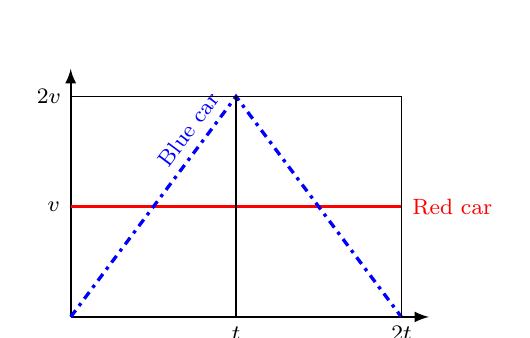
\begin{tikzpicture}[scale=.7]
        \draw[axes] (0,0)--(6.5,0);
        \draw[axes] (0,0)--(0,4.5);
        \draw[very thick,red] (0,2)--(6,2) node[pos=0,left,black]{$v$}
        node[right]{Red car};
        \draw[very thick,dash dot,blue] (0,0)--(3,4)
        node[pos=.8,above,sloped,dash dot,blue]{Blue car} --(6,0);
        \draw (0,4)--(6,4) node[pos=0,left]{$2v$};
        \draw (3,0)--(3,4) node[pos=0,below]{$t$};
        \draw (6,0)--(6,4) node[pos=0,below]{$2t$};
      \end{tikzpicture}
    \end{center}
    \begin{enumerate}[noitemsep]
    \item The blue car has travelled further, and both cars have the
      same instantaneous velocity
    \item Both cars have travelled the same distance, and the blue
      car has a greater instantaneous velocity
    \item The red car has travelled further, and both cars have the same
      instantaneous velocity
    \item Both cars have travelled the same distance, and both cars have the
      same instantaneous velocity
    \item The blue car has travelled further, and the blue car has a greater
      instantaneous velocity
    \end{enumerate}
    
  \item A car is travelling west and approaching a stop sign. As it is
    slowing to a stop, the directions associated with the object's velocity and
    acceleration, respectively, are
    \begin{enumerate}[noitemsep]
    \item West, East
    \item West, West
    \item East, East
    \item East, West
    \item There is not enough information to tell
    \end{enumerate}
    
  %\item The direction equivalent to [\ang{40} W of S] is
  %  \begin{enumerate}[noitemsep]
  %  \item [\ang{40} E of S]
  %  \item [\ang{40} W of N]
  %  \item [\ang{40} E of N]
  %  \item [\ang{50} S of W]
  %  \item [\ang{50} E of N]
  %  \end{enumerate}

  \item If a car travelling at \SI{60}{\kilo\metre\per\hour} [S] stops
    in a time of \SI{3.5}\second, its acceleration is:
    \begin{enumerate}[noitemsep]
    \item \SI{4.77}{\metre\per\second\squared} [S]
    \item \SI{4.77}{\metre\per\second\squared} [N]
    \item \SI{16.7}{\metre\per\second\squared} [S]
    \item \SI{16.7}{\metre\per\second\squared} [N]
    \item \SI{17.1}{\metre\per\second\squared} [S]
    \end{enumerate}

  \item Which of the following objects are in ``free fall''?
    \begin{enumerate}[noitemsep]
    \item A ball that was thrown horizontally
    \item A ball that was thrown at an angle above horizontal
    \item A ball that was thrown at an angle below horizontal
    \item A ball that was dropped
    \item All of the above
  \end{enumerate}
    
  \item An airplane is flying to a city due south from its current location. If
    there is a slight wind blowing to the south-east, the plane must head
    (point) to the:
    \begin{enumerate}[noitemsep]
    \item South
    \item West
    \item South-west
    \item South-east
    \item East
    \end{enumerate}

  \item A ball is thrown up in the air and then caught at the same height.
    The acceleration is \SI{9.81}{\metre\per\second\squared} [down]
    \begin{enumerate}[noitemsep]
    \item on the way up
    \item on the way down
    \item at the peak of its trajectory
    \item two of A, B, and C are correct
    \item all of A, B, and C are correct
  \end{enumerate}

  \item Two velocity vectors $v_1$ and $v_2$ each have the same magnitude.
    Graph 1 shows the velocity $v_1$ at $t=\SI0\second$, and then the same
    object has a velocity $v_2$ at $t=\SI2\second$, shown in Graph 2. Which of
    the following vectors best represents the average acceleration vector that
    causes the object's velocity to change from $v_1$ to $v_2$ ?
    \begin{center}
      \begin{tikzpicture}[scale=.6]
        \draw (-2,0)--(2,0);
        \draw (0,-2)--(0,2);
        \draw[vectors] (0,0)--(1.8,0) node[above]{$v_1$};
      \end{tikzpicture}
      \hspace{.2in}
      \begin{tikzpicture}[scale=.6]
        \draw (-2,0)--(2,0);
        \draw (0,-2)--(0,2);
        \draw[vectors] (0,0)--(0,1.8) node[right]{$v_2$};
      \end{tikzpicture}
    \end{center}
    A. \begin{tikzpicture}[scale=.6]
      \draw (-2,0)--(2,0);
      \draw (0,-2)--(0,2);
      \draw[vectors] (0,0)--(0,1.8);
    \end{tikzpicture}
    \hspace{.2in}
    B. \begin{tikzpicture}[scale=.6]
      \draw (-2,0)--(2,0);
      \draw (0,-2)--(0,2);
      \draw[vectors] (0,0)--(1.8,0);
    \end{tikzpicture}
    \hspace{.2in}
    C. \begin{tikzpicture}[scale=.6]
      \draw (-2,0)--(2,0);
      \draw (0,-2)--(0,2);
      \draw[vectors] (0,0)--(-1.8,0);
    \end{tikzpicture}
    \hspace{.2in}
    D. \begin{tikzpicture}[scale=.6]
      \draw (-2,0)--(2,0);
      \draw (0,-2)--(0,2);
      \draw[vectors,rotate=-45] (0,0)--(0,1.8);
    \end{tikzpicture}
    \hspace{.2in}
    E. \begin{tikzpicture}[scale=.6]
      \draw (-2,0)--(2,0);
      \draw (0,-2)--(0,2);
      \draw[vectors,rotate=45] (0,0)--(0,1.8);
    \end{tikzpicture}
  
  \item A passenger on a train moving horizontally at a constant speed
    relative to the ground drops a ball from his window. A stationary observer
    on the ground sees the ball falling with a speed $v_1$ at an angle to
    the vertical at an instant after it is dropped from the train window, but
    the ball appears to be falling vertically with a speed $v_2$ at the same
    instant as viewed by the train passenger. What is the speed (magnitude of
    velocity) of the train relative to the ground after the ball is dropped?
    Neglect air resistance.
    \begin{enumerate}[noitemsep]
    \item $v_1 + v_2$
    \item $v_1-v_2$
    \item $v_1^2 + v_2^2$
    \item $v_1^2-v_2^2$
    \item $\sqrt{v_1^2-v_2^2}$
    \end{enumerate}
    
  \item A ball is dropped from rest from the top of a cliff \SI{80}{\metre}
    high. At the same time, a rock is thrown horizontally from the top of the
    same cliff. The rock and ball hit the level ground below a distance of
    \SI{40}{\metre} apart. The horizontal velocity of the rock that was thrown
    was most nearly
    \begin{center}
      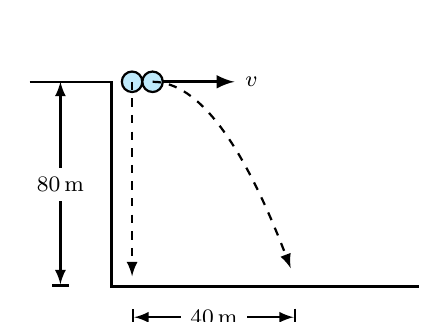
\begin{tikzpicture}[scale=1.3]
        \draw[thick] (-.8,0)--(0,0)--(0,-2)--(3,-2);
        \draw[thick,<->|](-.5,0)--(-.5,-2) node[midway,fill=white]{\SI{80}\metre};
        \draw[mass] (.2,0) circle (.1);
        \draw[mass] (.4,0) circle (.1);
        \draw[vectors] (.5,0)--(1.2,0) node[right]{$v$};
        \draw[axes,dashed] (.2,0)--(.2,-1.9);
        \draw[axes,dashed] plot[smooth,domain=.4:1.75] (\x, {-(\x-.4)^2});
        \draw[thick,|<->|] (.2,-2.3)--(1.8,-2.3)
        node[midway,fill=white]{\SI{40}\metre};
      \end{tikzpicture}
    \end{center}
    \begin{enumerate}[noitemsep]
    \item\SI5{\metre\per\second}
    \item\SI{10}{\metre\per\second}
    \item\SI{20}{\metre\per\second}
    \item\SI{40}{\metre\per\second}
    \item\SI{80}{\metre\per\second}
    \end{enumerate}
  
  \item A golf ball is hit from level ground and has a horizontal range of
    100 m. The ball leaves the golf club at an angle of \ang{60} to the level
    ground. At what other angle(s) can the ball be struck at the same initial
    velocity and still have a range of 100 m?
    \begin{center}
      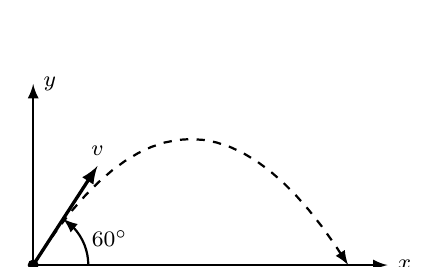
\begin{tikzpicture}
        \draw[axes] (0,0)--(4.5,0) node[right]{$x$};
        \draw[axes] (0,0)--(0,2.3) node[right]{$y$};
        \fill circle (.07);
        \draw[vectors,rotate=57] (0,0)--(1.5,0) node[above]{$v$};
        \draw[thick,dashed,->,domain=0:4] plot(\x,{-.4*((\x-2)*(\x-2))+1.6});
        \draw[axes] (.7,0) arc (0:57:.7) node[midway,right]{\ang{60}};
      \end{tikzpicture}
    \end{center}
    \begin{enumerate}[noitemsep]
    \item\ang{30}
    \item\ang{20} and \ang{80}
    \item\ang{10} and \ang{120}
    \item\ang{45} and \ang{135}
    \item There is no other angle other than \ang{60} in which the ball will
      have a range of 100 m.
  \end{enumerate}
  
  \item The motion of an object is represented by the acceleration vs.\ time
    graph below. If the object is initially at rest, which of the
    following statements is true about its motion?
    \begin{center}
      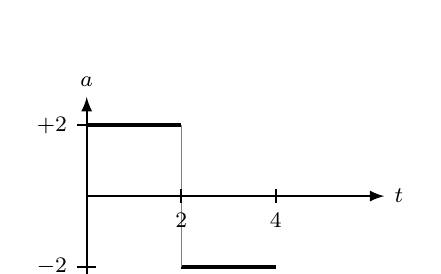
\begin{tikzpicture}[yscale=.45,xscale=.6]
        \draw[axes] (0,0)--(6.3,0) node[right]{$t$};
        \draw[axes] (0,-2.5)--(0,2.8) node[above]{$a$};
        \draw[ultra thick] (0,2)--(2,2);
        \draw[ultra thick] (2,-2)--(4,-2);
        \draw[gray] (2,2)--(2,-2);
        \draw[thick] (2,.2)--(2,-.2) node[below]{2};
        \draw[thick] (4,.2)--(4,-.2) node[below]{4};
        \draw[thick] (.2,2)--(-.2,2) node[left]{$+2$};
        \draw[thick] (.2,-2)--(-.2,-2) node[left]{$-2$};
      \end{tikzpicture}
    \end{center}
    \begin{enumerate}[noitemsep]
    \item The object returns to its original position.
    \item The velocity of the object is zero at a time of \SI2\second.
    \item The velocity of the object is zero at a time of \SI4\second.
    \item The displacement of the object is zero at a time of \SI4\second.
    \item The acceleration of the object is zero at a time of \SI2\second.
    \end{enumerate}
    
  \item Can an object ever be accelerating and experiencing an
    instantaneous velocity of \SI0{\metre\per\second}? Explain. 
    
  \item Large insects such as locusts can jump as far as \SI{75}{cm}
    horizontally on a level surface. An entomologist analyzed a photograph and
    found that the insect's launch angle was \ang{55}. What was the insect's
    initial velocity?
  
  \item Because of an oncoming storm, a boat must cross a river in the
    shortest amount of time possible regardless of where it lands on the
    opposite shore. Given that the river has a current, in what direction
    should the boat point? Explain.
    \vspace{\stretch1}
  
  \item While hiking in the wilderness, you come to the top of a cliff that
    is \SI{60}{\metre} high. You throw a stone from the cliff, giving it an
    initial velocity of \SI{21}{\metre\per\second} at \ang{35} above the
    horizontal. How far from the base of the cliff does the stone land?
    \vspace{\stretch2}
  
  \item You want to shoot a stone with a sling shot and hit a target on the
    ground \SI{14.6}{\metre} away. If you give the stone an initial speed of
    \SI{12.5}{\metre\per\second}, neglecting friction and air resistance, what
    is/are the launch angle(s) in order for the stone to hit the target? What
    would be the maximum height(s) by the stone? What would be its time of
    flight? Assume motion is symmetric.
  
  \item A sharpshooter shoots a bullet horizontally over level ground with
    a velocity of \SI{1.22e3}{\metre\per\second}. At the instant that the bullet
    leaves the barrel, its empty shell casing falls vertically and strikes the
    ground with a vertical velocity of \SI{5.50}{\metre\per\second}.
    \begin{enumerate}
      \item Neglecting air friction, how far does the bullet travel?
      \item What is the vertical component of the bullet's velocity at the
      instant before it hits the ground?
    \end{enumerate}

  \item A projectile is launched from point $O$ at an angle of \ang{22} with
    an initial velocity of $v_0=\SI{15}{\metre\per\second}$ up an incline plane
    that makes an angle of \ang{10} with the horizontal. The projectile lands on
    the incline plane at point $M$.
    \begin{center}
      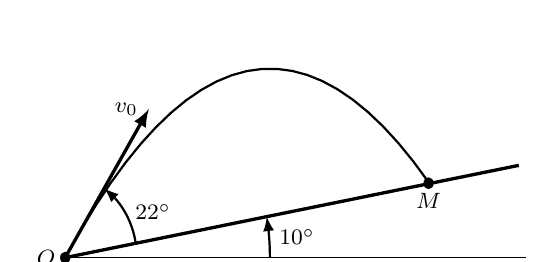
\begin{tikzpicture}[xscale=1.3,yscale=1.5]
        \draw (0,0)--(4.5,0);
        \fill circle (.05) node[left]{$O$};
        \draw[vectors,rotate=57] (0,0)--(1.5,0) node[left]{$v_0$};
        \draw[thick,domain=0:3.55] plot(\x,{-.4*((\x-2)*(\x-2))+1.6});
        \draw[axes,rotate=10] (.7,0) arc(0:47:.7) node[midway,right]{\ang{22}};
        \draw[very thick,rotate=10] (0,0)--(4.5,0);
        \draw[axes] (2,0) arc (0:10:2) node[midway,right]{\ang{10}};
        \fill (3.55,.63) circle (.05) node[below]{$M$};
      \end{tikzpicture}
    \end{center}
    \begin{enumerate}
      \item Find the time it takes for the projectile to hit the incline plane.
      \item Find the distance $OM$.
    \end{enumerate}
    
  \item A baseball is thrown by an outfielder ($O$) towards the catcher
    ($C$) with an initial speed of \SI{20}{\metre\per\second} at an angle of
    \ang{45} with the horizontal. At the moment that the ball is thrown, $C$ is
    \SI{50}{\metre} from $O$. At what speed and in what direction must $C$ run
    to catch the ball at the same height at which it was released? Assume that
    $C$ catches the ball at the same moment that it arrives. Please answer in
    two significant figures.

  \item A car is travelling north on a city street at
    \SI{12.5}{\metre\per\second}. Just as the car crosses a perpendicularly
    intersecting crossroad, the passenger throws out a can horizontally, towards
    the east. The initial speed of the can relative to the car is
    \SI{10.0}{\metre\per\second}. It is released at a height of 1.75 m above the
    road.
    \begin{enumerate}
      \item What is the initial velocity of the can relative to the road?
      \item Where does the can land relative to the centre of the intersection?
    \end{enumerate}
  
%  %\item An object is thrown upward on a slope and reached a height of
%  %$h=\SI{15}{\metre}$ as shown, the object lands near the base of slope at a
%  %distance of $l=\SI{75}{\metre}$ away. The slope angle $\alpha$ is \ang{35}.
%  %\begin{center}
%  %  \pic{.35}{../graphics/FF55a}
%  %\end{center}
%  %Determine
%  %\begin{parts}
%  %\item the magnitude $v$, and
%  %\item the direction of the initial velocity $\theta$
%  %\end{parts}
  \end{enumerate}
\end{multicols}

%
%%\usetikzlibrary{decorations.pathmorphing,patterns}

\chapter{Dynamics}
\label{chapter:dynamics}

%\section[Intro]{Introduction}

Now that we can mathematically describe the motion of any object, we have to
be able describe \emph{what} causes motion, or more precisely,
\emph{what causes motion to change.}




\section{Laws of Motions}
The definitions given here are based on the original text by Newton in
\emph{Principia}, but with some wording replaced with modern physics
language\footnote{For example, Newton used the term \emph{the alteration of
motion} to describe the acceleration of the object.}

The first law of motion describes what happens when there are no forces act on
an object:
\begin{definition}
  \textbf{First law:} Every object remains at rest or in uniform motion, until
  there is a net external force acting on the object.
\end{definition}
In other words, when the vector sum of all the forces acting on an object is
zero, the object's velocity does not change. In other words, the three equations
below are equivalent:
\begin{equation*}
  \bm F_\text{net}=\sum\bm F=\bm 0
  \quad\longleftrightarrow\quad
  \bm v=\text{constant}
  \quad\longleftrightarrow\quad
  \bm a=\bm 0
\end{equation*}
%  \end{center}
%  \begin{itemize}
%  \item As long as an object moves in uniform motion, it must be that
%    $\bm F_\text{net}=\bm 0$
%  \item Examples:
%    \begin{itemize}
%    \item A spacecraft in ``deep space'' has no forces acting on it
%    \item A hockey puck sliding on very smooth ice has gravity and normal
%      force, but the net force is zero
%    \item A car travelling on a highway at \SI{100}{\kilo\metre\per\hour} has
%      many forces acting on it, but the net force is zero
%    \end{itemize}
%  \item In ``a state of equilibrium''
%  \end{itemize}

What is not stated explicitly by Newton is that the first law of motion is only
valid when the mass of the object is constant. In other words, the first law of
motion, as stated above, will \emph{not} work for:
\begin{itemize}[itemsep=3pt]
\item A rocket expelling spent fuel as it is launched towards space
\item A train car collecting grain though its open top
\end{itemize}
Later in Chapter~\ref{chapter:momentum}, we will modify the first law of motion
to include objects with changing mass.


The secon law of motion addresses what happens when the forces acting on an
object is not balance, i.e.\ when the net force is not zero.

\begin{definition}
  \textbf{Second law:} The acceleration of an object is proportional to the
  sum of all forces (net force) acting on it; and is along the same
  direction as the net force.
\end{definition}
The second law states that the acceleration of an object is the directresult of
the imbalance of forces, and that the relationship is \emph{linear} (i.e.\ when
the net force is double, the acceleration also doubles).

The first two laws of motion can be summarized by perhaps one of the most
important and recognizable equations in physics:
\begin{equation}
  \boxed{\bm F_\text{net}=m\bm a}
\end{equation}
The \emph{proportionality} between the net force and the acceleration of the
object is its mass. In fact, mass is defined as the ratio between the magnitude
of the net force acting on an object and the magnitude of the resultant
acceleration:
\begin{equation}
  m=\frac{|\bm F_\text{net}|}{|\bm a|}
\end{equation}
As such, mass is an intrinsic property of an object, and the same net force on
the object will \emph{always} result in the same acceleration, regardless of
what the net force is composed of, and whether the object is on Earth, on the
Moon, or in deep space.

Both the first and second laws of moton, as stated by Newton, require that the
mass of the object be constant. 




The third law of motion deals with the interaction between objects when forces
are created, and how objects apply forces on each other:
\begin{definition}
  \textbf{Third Law:} To every action there is always opposed and equal
  reaction; the mutual actions of two bodies upon each other are always
  equal, and directed to contrary parts.
\end{definition}
Mathematically, we can write that the force object $A$  exerts on bbject $B$
($\bm F_{AB}$, the action force) is equal in magnitude but opposite in
direction to the force that object $B$ exerts on object $A$ ($\bm F_{BA}$, the
reaction force).
\begin{equation}
  \boxed{\bm F_\text{AB} = -\bm F_\text{BA}}
  \label{eq:third-law}
\end{equation}
The negative sign in Eq.~\ref{eq:third-law} indicates that the forces are in
opposite direction. It must be noted that
\textbf{the action and reaction forces must act on \emph{different} objects}.

The implication of the laws of motion is that forces are always created in
pairs: it is impossible for one object to exert a force on another without also
simultaneously being acted on by the other object. In
Chapter~\ref{chapter:energy}, we will show that the third law of motion is
crucial in formulating, and understanding, the law of conservation of energy.
In Chapter~\ref{chapter:momentum}, we will show that the third law of motion
is, in fact, an application of the first law of motion.

%\begin{example}
%  Old-style television picture tubes and computer monitors use cathode ray
%  tubes, where light is produced when fast-moving electrons collide with
%  phosphor molecules on the surface of the screen. The electrons (mass
%  $m=\text{\SI{9.1e-31}{\kilo\gram}}$) are accelerated from rest in the
%  electron ``gun'' at the back of the vacuum tube. Find the velocity of an
%  electron when it exits the gun after experiencing an electric force of
%  \SI{5.8e-15}{\newton} over a distance of \SI{3.5}{\milli\metre}.
%\end{example}

\section{Common Forces}
%  \textbf{Force} is the interaction between the objects
%  \begin{itemize}
%  \item When there is interaction, then forces are created
%  \item A ``push'' or a ``pull''
%  \end{itemize}
%
%  \vspace{.2in}There are two types of forces:
%  \begin{itemize}
%  \item\textbf{Contact forces} act between two objects that are in contact
%    with one another
%  \item\textbf{Non-contact forces} act between two objects without them
%    touching each other.
%    \begin{itemize}
%    \item Also called ``action-at-a-distance'' force
%    \end{itemize}
%  \end{itemize}
%
%
%
%
%\section{Forces}
%  Newton considered all forces acting at a single point of an object called the
%  centre of mass (``CM'')
%  \begin{itemize}
%  \item The centre of mass is also called the centre of gravity (``CG'') if the
%    object is inside a uniform gravitational field\footnote{Gravitational field
%    is a topic that will be discussed in Class 7}
%  \item If the density of an object is constant, then the CM is also the
%    geometric centre (centroid) of the object
%  \end{itemize}
%%  \vspace{.2in}If the net force on an object is zero ($\sum\bm F=\bm{0}$)
%%  then the object is in a \emph{state of equilibrium}
%%  \begin{itemize}
%%  \item Dynamic equilibrium: the object is moving relative to us
%%  \item Static equilibrium: the object is not moving relative to us
%%  \end{itemize}




\begin{itemize}[noitemsep]
\item Gravitational force ($\bm F_g$)
\item Normal force ($\bm F_n$)
\item Static and kinetic friction ($\bm F_s$ and  $\bm F_k$)
\item Spring force ($\bm F_e$)
\item Tension ($\bm F_T$)
\item Fluid Resistance, or Drag ($\bm F_d$)
\item Applied force ($\bm F_a$)
\item Electrostatic force ($\bm F_q$, discussed in Unit 3)
\item Magnetic force ($\bm F_m$, discussed in Unit 3)
\end{itemize}




\subsection{Gravity}
\textbf{Gravity} is the mutual force of attraction between all massive objects.
The gravitational force that objects apply to each other can be expressed as:
\begin{equation}
  \boxed{\bm F_g=m\bm g}
\end{equation}
The gravitational force acts in the same direction as $\bm g$, the acceleration
due to gravity at the object's position. At or near the surface of Earth,
$\bm g=\text{\SI{9.81}{\metre\per\second\squared}}$ [down]. In fact, the
direction of $\bm g$ is how we \emph{define} the concept of ``down''. $\bm g$
is also known as the ``gravitational field''; will be discussed in depth in
Chapter~\ref{chapter:gravity}. If this is the only force that acts on an object,
its resulting motion is called \textbf{free fall}.

To be clear, by the third law of motion, any object that is subjected to the
gravitational pulled by Earth will also exert an equal and opposite force on
Earth. However, since Earth is much more massive, this force will have no
effect to Earth's motion.

\subsection{Normal Force}
\textbf{Normal force} $F_n$ is a force a surface exerts on another object
that it is in contact with. It is always \emph{perpendicular} to the contact
surface.\footnote{This is where the term \emph{normal} came from.}

\begin{figure}[ht]
  \centering
  \begin{tikzpicture}
    \draw[thick] (-1,0)--(2.5,0);
    \draw[mass] rectangle (1.5,1);
    \fill (.75,.5) circle (2pt);
    \draw[vectors] (.75,.5)--+(0,-1) node[below]{$F_g$};
    \draw[vectors] (.75,.5)--+(0,1) node[above]{$F_n$};
  \end{tikzpicture}
  \hspace{.5in}
  \begin{tikzpicture}
    \begin{scope}[rotate=30]
      \draw[thick] (-1,0)--(2.5,0);
      \draw[mass] rectangle (1.5,1);
      \fill (.75,.5) circle (2pt);
      \begin{scope}[vectors]
        \draw[rotate around={-30:(.75,.5)}] (.75,.5)--+(0,-1)
        node[below]{$F_g$};
        \draw (.75,.5)--+(0,1) node[above]{$F_n$};
      \end{scope}
    \end{scope}
  \end{tikzpicture}
\end{figure}
Regardless of whether the surface is horizontal or slanted, $F_n$ is always be
perpendicular to the surface. However, the \emph{magnitude} of the normal force
will change.




%%\section{Normal Force on an Incline}
%%  When an object sits on a stationary incline, normal force decreases.
%%  
%%    \centering
%%    \begin{tikzpicture}[scale=.9]
%%      \draw[thick] (-1,0)--(3,0);
%%      \draw[thick,->] (0,0) arc (0:37:1) node[midway,right] {$\theta$};
%%      \begin{scope}[rotate around={37:(-1,0)}]
%%        \draw[->](3.5,.5)--(4,.5)  node[right]{$x$};
%%        \draw[->](3.5,.5)--(3.5,1) node[above]{$y$};
%%        \draw[thick] (-1,0)--(4,0);
%%        \draw[fill=pink,thick] rectangle (3,2);
%%        \fill(1.5,1) circle (.07) node[right]{CM};
%%        \begin{scope}[->,thick,red]
%%          \draw[dotted] (1.5,1)--(1.5,-.5) node[right]{$F_g\cos\theta$};
%%          \draw[dotted] (1.5,1)--(.45,1) node[left]{$F_g\sin\theta$};
%%        \end{scope}
%%        \draw[->,very thick,red] (1.5,1)--(.45,-.5)
%%        node[below]{$F_g$}
%%        node[pos=.3,below right]{$\theta$};
%%        \draw[->,very thick] (1.5,1)--(1.5,2.5) node[above]{$F_n$};
%%      \end{scope}
%%    \end{tikzpicture}
%%    
%%    \begin{itemize}
%%    \item $F_n=F_g\cos\theta$
%%    \item $F_g$ has a component along the ramp $F_g\sin\theta$ that
%%      wants to slide the block down.
%%    \item There may also be a friction force $F_f$ that opposes the motion
%%    \item If the incline is also accelerating, then we have to treat this
%%      problem as a connected-body problem (discussed later in this topic)
%%    \end{itemize}

\subsection{Friction}
\textbf{Friction} is force that opposes the sliding of two surface across one
another
\begin{itemize}
\item Always act in the direction opposite to motion or attempted motion
\item Two types: \emph{static friction} and \emph{kinetic friction}
\end{itemize}  
%  \begin{center}
%   \pic{.6}{graphics/friction}
%  \end{center}


\textbf{Static friction} is the resistive force between two surfaces when
there is no relative motion between them. It increases with increasing
applied force $F_a$. It is at maximum when the object is just about to move.
\begin{equation}
  \boxed{
    F_s \leq \mu_sF_n
  }
  \label{eq:static-friction}
\end{equation}
\begin{center}
  \begin{tabular}{l|c|c}
    \rowcolor{pink}
    \textbf{Quantity} & \textbf{Symbol} & \textbf{SI Unit} \\ \hline
    Magnitude of static friction   & $F_s$ & \si\newton \\
    Coefficient of static friction & $\mu_s$ & (no unit)\\
    Magnitude of normal force      & $F_n$ & \si\newton
  \end{tabular}
\end{center}
Equation~\ref{eq:static-friction} only deals with the \emph{magnitude} of the
force. A proper free-body diagram is required to express the direction of
$\bm F_s$
%  \begin{tikzpicture}[overlay]
%    \uncover<2>{
%      \node[text width=85,draw=violet,fill=violet!5,text=violet] (act) at
%      (-3.2,4) {Actual static friction};
%      \draw[axes,violet] (act)--+(3,0);
%      
%      \node[text width=100,draw=orange,fill=orange!5,text=orange] (max) at
%      (5.05,4) {Maximum static friction};
%      \draw[axes,orange] (max)--+(-3,0);
%    }
%  \end{tikzpicture}

\textbf{Kinetic friction} is the resistive force between two surfaces that
are moving relative to each other. It is (nearly) constant along the path of
movement as long as the normal force stays constant:
\begin{equation}  
  \boxed{F_k = \mu_kF_n}
\end{equation}
\begin{center}
  \begin{tabular}{l|c|c}
    \rowcolor{pink}
    \textbf{Quantity} & \textbf{Symbol} & \textbf{SI Unit} \\ \hline
    Magnitude of kinetic friction   & $F_k$   & \si{\newton}\\
    Coefficient of kinetic friction & $\mu_k$ & (no unit)\\
    Magnitude of normal force       & $F_n$   & \si{\newton}
  \end{tabular}
\end{center}    
$\mu_k$ is always lower than $\mu_s$, otherwise nothing will ever move:
\begin{equation}  
  \mu_k\leq\mu_s
\end{equation}

%  \begin{tikzpicture}[overlay]
%    \uncover<2>{
%      \node[text width=86,draw=magenta,fill=magenta!5,text=magenta] (act) at
%      (3.5,5) {Unlike static friction, this is an equality};
%      \draw[axes,magenta] (act) to[out=50,in=90] +(3.5,.25);
%    }
%  \end{tikzpicture}




\subsection{Tension in a Cable}
\textbf{Tension} is the force exerted on and by a cable, rope, or string.
\begin{itemize}
\item You can't push on a rope
\item Assume the cable/rope/string to be mass less
\item Force can change direction when used with pulleys
\end{itemize}
How do engineers determine the amount of tension needed for a specific object
(bridges, floors or light fixtures)?




\subsection{Spring Force}
The spring force $\bm F_e$ is the force that a compressed/stretched spring
exerts on the object connected to it. An \emph{ideal} spring obeys
\textbf{Hooke's law}:
\begin{equation}
  \boxed{
    \bm F_e=-k\bm x
  }
\end{equation}
$\bm F_e$ is in the opposite direction to the spring's displacement $\bm x$,
and is proportional to the amount of compression/stretching.

\begin{center}
  \begin{tikzpicture}[scale=.8]
    \draw[mass] (5,.5) rectangle (6,1.5);
    \draw[thick,
      decoration={aspect=.6,segment length=5mm, amplitude=2.5mm, coil},
      decorate] (0,1)--(5,1);
    \fill[pattern=north east lines](-.2,0) rectangle (0,2);
    \draw[thick] (0,0)--(0,2);
    \fill[red] (5.5,1) circle (.06);
    \draw[vectors,red] (5.5,1)--(4,1) node[above]{$\bm F_e$};
    \draw[dashed] (3,0)--(3,2) node[above]{Equilibrium position};
    \draw[vectors] (3,.3)--(5,.3) node[midway,below]{$x$};
  \end{tikzpicture}
  \hspace{.2in}
  \begin{tikzpicture}[scale=.8]
    \draw[thick,gray!40,fill=gray!20] (5,.5) rectangle (6,1.5);
    \draw[thick,gray!20,
      decoration={aspect=.6,segment length=5mm, amplitude=2.5mm, coil},
      decorate] (0,1)--(5,1);
    \fill[pattern=north east lines] (-.2,0) rectangle(0,2);
    \draw[thick] (0,0)--(0,2);
    \fill[gray!30] (5.5,1) circle (.06);
    \draw[vectors,gray!30] (5.5,1)--(4,1) node[above]{$\bm F_e$};
    \draw[dashed] (3,0)--(3,2);
    \draw[vectors,gray!30] (3,.3)--(5,.3) node[midway,below]{$x$};
    \draw[mass] (1.5,.5) rectangle (2.5,1.5);
    \draw[thick,
      decoration={aspect=.3,segment length=1.5mm, amplitude=2.5mm, coil},
      decorate] (0,1)--(1.5,1);
    \draw[vectors] (3,.3)--(1.5,.3) node[midway,below]{$x$};
    \fill[red] (2,1) circle (.06);
    \draw[vectors,red] (2,1)--(3,1) node[above]{$\bm F_e$};
  \end{tikzpicture}
\end{center}
The constant $k$ (called the \textbf{spring constant}, \textbf{force
  constant}, \textbf{Hooke's constant} or \textbf{spring rate}) is the
stiffness of the spring. It has a unit of \si{\newton\per\metre}.



\subsection{Fluid Resistance (Drag)}

When an object (e.g.\ an aircraft, a bicycle or a car) moves through air, or
when a submarine moves under water, they all experience a
fluid\footnote{A gas or a liquid} resistance force called the
\textbf{drag} $\bm F_d$.
\begin{figure}[ht]
  \centering
  \begin{subfigure}{.338\textwidth}
    \pic1{dynamics/boeing787}
    \caption{A commercial aircraft flying through air}
  \end{subfigure}
  \begin{subfigure}{.35\textwidth}
    \pic1{dynamics/ganna}
    \caption{A cyclist riding at high speed during a bike race}
  \end{subfigure}
  \begin{subfigure}{.263\textwidth}
    \pic1{dynamics/submarine}
    \caption{A submarine moving through water}
  \end{subfigure}
\end{figure}
The drag force is experienced by any object moving through a fluid. The
direction of drag is in the opposite direction to the velocity vector.

There are multiple sources of drag:
\begin{itemize}
\item\textbf{form drag} is due to the shape of the object
\item\textbf{skin friction} is due to the friction of the fluid against
  the surface of the object moving through it
\item\textbf{interference drag} is due to when airflow around one part of
  an object occupying the same space as the airflow around another part
  (e.g.\ fuselage and wing of an airplane)
\end{itemize}

Unlike kinetic friction (which is constant), drag depend on the speed of the
moving object, as well as its shape:
\begin{equation}
  \boxed{
    F_d=\frac12\rho v_\infty^2C_DA_\text{ref}
  }
\end{equation}
\begin{center}
  \begin{tabular}{l|c|c}
    \rowcolor{pink}
    \textbf{Quantity} & \textbf{Symbol} & \textbf{SI Unit} \\ \hline
    Magnitude of drag       & $F_d$     & \si\newton \\
    Density of the fluid    & $\rho$    & \si{\kilo\gram\per\metre\cubed}\\
    Free-stream velocity    & $v_\infty$ & \si{\metre\per\second} \\
    Reference area          & $A_\text{ref}$ & \si{\metre\squared} \\
    Drag coefficient        & $C_D$     & (no unit)
  \end{tabular}
\end{center}
$C_D$ depends on the shape and surface smoothness of the object; for bluff
bodies $A_\text{ref}$ is the frontal area; for streamlined objects
$A_\text{ref}$ is the planform (top-view) area




\section{Free Body Diagrams}
A free-body diagram is used to visualize the forces acting on an object. It is
very useful tool that should be used all the time.
\emph{We generally draw the forces from an inertial frame of reference.}

\begin{enumerate}
\item Draw a ``big dot'' to represent the centre of mass of the object.
%  \vspace{.1in}
%  
%    \centering
%    \begin{tikzpicture}[scale=.8]
%      \draw[lightgray,thick] (-1,0)--(4,0);
%      \draw[lightgray,fill=cyan!10,thick] rectangle (3,2);
%      \fill (1.5,1) circle (.1) node[above]{CM};
%    \end{tikzpicture}
%    
%    \centering
%    \begin{tikzpicture}[scale=.8]
%      \begin{scope}[rotate=30]
%        \draw[lightgray,thick] (0,0)--(5,0);
%        \draw[lightgray,fill=cyan!10,thick] (1,0) rectangle (4,2);
%        \fill (2.5,1) circle (.1) node[above]{CM};
%      \end{scope}
%      \draw[lightgray,thick] (0,0)--(4.5,0);
%    \end{tikzpicture}
%    
%    \centering
%    \begin{tikzpicture}[scale=.8]
%      \draw[lightgray,fill=cyan!10,thick] circle (.5);
%      \fill circle (.1) node[above]{CM};
%    \end{tikzpicture}
%  
%
%
%
%
%\section{Free Body Diagrams}
\item Define a coordinate system ($x$ and $y$ axes)
  \begin{itemize}
  \item Axes are defined to simplify the problem (not to make it more
    complicated!)
  \item Define coordinate system such that motion is along one axis (usually
    $x$) only
  \end{itemize}

%  \vspace{.1in}
%  
%    \centering
%    \begin{tikzpicture}[scale=.8]
%      \draw[lightgray,thick] (-1,0)--(4,0);
%      \draw[lightgray,fill=cyan!10,thick] rectangle (3,2);
%      \fill (1.5,1) circle (.1);
%      \draw[axes] (3.5,.5)--(4.5,.5) node[right]{$x$};
%      \draw[axes] (3.5,.5)--(3.5,1.5) node[above]{$y$};
%    \end{tikzpicture}
%    
%    \centering
%    \begin{tikzpicture}[scale=.8]
%      \begin{scope}[rotate=30]
%        \draw[lightgray,thick] (0,0)--(5,0);
%        \draw[lightgray,fill=cyan!10,thick] (1,0) rectangle (4,2);
%        \fill (2.5,1) circle (.1);
%        \draw[axes] (4.5,.5)--(5.5,.5)  node[right]{$x$};
%        \draw[axes] (4.5,.5)--(4.5,1.5) node[above]{$y$};
%      \end{scope}
%      \draw[lightgray,thick] (0,0)--(4.5,0);
%    \end{tikzpicture}
%    
%    \centering
%    \begin{tikzpicture}[scale=.8]
%      \draw[lightgray,fill=cyan!10,thick] circle (.5);
%      \fill circle (.1);
%      \draw[axes] (1,0)--(2,0) node[right]{$x$};
%      \draw[axes] (1,0)--(1,1) node[above]{$y$};
%    \end{tikzpicture}
%
%
%
%
%
%\section{Free Body Diagrams}
\item Identify and label all forces acting on the object
  \begin{itemize}
  \item If it has mass, weight $\bm F_g$ acts downward
  \item If it is on a surface, there is also a normal force $\bm F_n$
  \item If there is friction, first think about which direction the object will
    move without it, then draw $\bm F_s$ or $\bm F_k$ in the opposite
    direction
  \item If it is being pushed/pulled, there may be an applied force
    $\bm F_a$ or tension force $\bm F_T$
  \end{itemize}

%  
%    \centering
%    \begin{tikzpicture}[scale=.8]
%      \draw[lightgray,thick] (-1,0)--(4,0);
%      \draw[lightgray,fill=cyan!10,thick] rectangle (3,2);
%      \fill (1.5,1) circle (.1);
%      \draw[axes] (3.5,.5)--(4.5,.5) node[right]{$x$};
%      \draw[axes] (3.5,.5)--(3.5,1.5) node[above]{$y$};
%      \draw[vectors] (1.5,1)--(1.5,-.5) node[below]{$\bm F_g$};
%      \draw[vectors] (1.5,1)--(1.5,2.5) node[above]{$\bm F_n$};
%      \draw[vectors] (1.5,1)--(3.1,1) node[below]{$\bm F_a$};
%      \draw[vectors] (1.5,1)--(.75,1) node[left]{$\bm F_f$};
%    \end{tikzpicture}
%    
%    \centering
%    \begin{tikzpicture}[scale=.8]
%      \draw[lightgray,thick] (0,0)--(4.5,0);
%      \begin{scope}[rotate=30]
%        \draw[lightgray,thick] (0,0)--(5,0);
%        \draw[lightgray,fill=cyan!10,thick] (1,0) rectangle (4,2);
%        \fill (2.5,1) circle (.1);
%        \draw[axes] (4.5,.5)--+(1,0) node[right]{$x$};
%        \draw[axes] (4.5,.5)--+(0,1) node[above]{$y$};
%        \draw[vectors,rotate around={-30:(2.5,1)}] (2.5,1)--(2.5,-.5)
%        node[below]{$\bm F_g$};
%        \draw[vectors] (2.5,1)--(2.5,2.4) node[above]{$\bm F_n$};
%        \draw[vectors] (2.5,1)--(4.1,1) node[below]{$\bm F_a$};
%        \draw[vectors] (2.5,1)--(1.75,1) node[left]{$\bm F_f$};
%      \end{scope}
%    \end{tikzpicture}
%    
%    \centering
%    \begin{tikzpicture}[scale=.8]
%      \draw[lightgray,fill=cyan!10,thick] circle (.5);
%      \fill circle (.1);
%      \draw[axes] (1,0)--(2,0) node[right]{$x$};
%      \draw[axes] (1,0)--(1,1) node[above]{$y$};
%      \draw[vectors] (0,0)--(0,-1.5) node[below]{$\bm F_g$};
%    \end{tikzpicture}
\end{enumerate}  


\section{Examples of Free Body Diagrams}



\section{Solving Force Problem}
Once the free-body diagram has been drawn,
\begin{itemize}
\item Break down the forces into the $x$ and $y$ components
\item Sum forces in the direction that doesn't have a net force (usually
  $y$ axis)
\item Sum forces in the other axis, and find out what the acceleration is
\item Use kinematic equations to solve the motion of the object along that axis
\end{itemize}




\begin{example}
  To move a \SI{45}{\kilo\gram} wooden crate across a wooden floor
  ($\mu=0.20$), you tie a rope onto the crate and pull on the rope. While you
  are pulling the rope with a force of \SI{115}\newton, it makes an angle of
  \ang{15} with the horizontal. How much time elapses between the time at which
  the crate just starts to move and the time at which you are pulling it with a
  velocity of \SI{1.4}{\metre\per\second}?
%  \begin{center}
%    \pic{.4}{graphics/pull-box}
%  \end{center}
\end{example}

\begin{example}
  You are holding an \SI{85}{\kilo\gram} trunk at the top of a ramp that slopes
  from a moving van to the ground, making an angle of \ang{35} with the ground.
  You lose your grip and the trunk begins to slide.
  \begin{enumerate}
  \item If the coefficient of friction between the trunk and the ramp is 0.42,
    what is the acceleration of the trunk?
  \item If the trunk slides \SI{1.3}{\metre} before reaching the bottom of the
    ramp, for what time interval did it slide?
  \end{enumerate}
\end{example}

\begin{example}
  A \SI{55}{\kilo\gram} person is standing on a scale in an elevator. If the
  scale is calibrated in \emph{newtons}, what is the reading on the scale when
  the elevator is not moving? If the elevator begins to accelerate upward at
  \SI{.75}{\metre\per\second\squared}, what will be the reading on the scale?
\end{example}



\begin{example}
  An elevator filled with people has a total mass of \SI{2245}{\kilo\gram}. As
  the elevator begins to rise, the acceleration is
  \SI{.55}{\metre\per\second\squared}. What is the tension in the cable that is
  lifting the elevator?   
\end{example}



\section{Multi-Body Problems}
\begin{figure}[ht]
  \centering
  \pic1{dynamics/graphics/go-train}
  \caption{A train in motion can be treated as a single object, or a number of
    objects connected together.}
\end{figure}
%\begin{center}
%  \pic{.7}{graphics/worldslongestroadtrainwithpowertrailer8}
%\end{center}
%  \begin{itemize}
%  \item Usually the objects are connected by a cable or a solid linkage with
%    negligible mass
%  \item All objects have the same acceleration
%  \item Require multiple free-body diagrams
%  \end{itemize}
%
%
%
%
%\section{Solving Connected-Bodies Problems}
%  To solve a connected-bodies problem, you can follow these procedures:
%  \begin{enumerate}
%  \item Draw a free-body diagram (FBD) on each of the objects
%  \item Sum all the forces on all the objects along the direction of motion
%    \begin{itemize}
%    \item Direction of motion is usually very obvious
%    \item Action/reaction pairs of forces cancel, because they are
%      \emph{internal} forces %and not \emph{external} forces
%    \end{itemize}
%  \item Compute the acceleration of the entire system using the second law of
%    motion
%    \begin{itemize}
%    \item Remember that every object has the same acceleration!
%    \end{itemize}
%  \item Go back to the FBD of each of the objects and compute any unknown
%    forces
%  \end{enumerate}
%
%
%
%
\subsection{Objects Connected by Cables}
\begin{example}
  Three masses ($m_1$, $m_2$ and $m_3$) are connected by massless cables (we
  assume that he cables are very light compared to the masses, and so we can
  ignore them without making our answers inaccurate), and pulled to the right
  by an applied force $\bm F$ across a level surface. The coefficient of
  kinetic friction between the masses and the surface is $\mu$.
  \begin{center}
    \begin{tikzpicture}
      \draw[thick] (0,0)--(11,0);
      \draw[mass] (1,0) rectangle (2.5,1) node[midway]{$m_3$};
      \draw[brown,line width=2] (2.5,.5)--(4,.5) node[midway,above]{$T_2$};
      \draw[mass] (4,0) rectangle (5.5,1) node[midway]{$m_2$};
      \draw[brown,line width=2] (5.5,.5)--(7,.5) node[midway,above]{$T_1$};
      \draw[mass] (7,0) rectangle (8.5,1) node[midway]{$m_1$};
      \draw[vectors] (8.5,.5)--(10,.5) node[right]{$\bm F$};
    \end{tikzpicture}
  \end{center}
  \begin{enumerate}
  \item What are the forces acting on each of the masses?
  \item What is the acceleration of the system,
    {\color{blue}assuming that the cables to not break?}
  \item What are the magnitudes of the tension forces ($T_1$ and $T_2$) in the
    cables?
  \end{enumerate}
\end{example}



\begin{example}
  Two masses ($m_1$ and $m_2$) are stacked on top of each other above a
  frictionless table. An external force $\bm F$ is applied to $m_2$, causing
  both blocks to accelerate to the right without slipping. The coefficients of
  friction between the masses is $\mu$.
  \begin{center}
    \begin{tikzpicture}
      \draw[thick] (-1,0)--(5.5,0);
      \draw[mass] rectangle (3,1) node[midway]{$m_2$};
      \draw[mass] (.75,1) rectangle (2.25,1.75) node[midway]{$m_1$};
      \draw[vectors] (3,.5)--(4.5,.5) node[right]{$\bm F$};
    \end{tikzpicture}
  \end{center}
  \begin{enumerate}
  \item What is the maximum acceleration of the masses without slipping?
  \item What is the magnitude of the external force $F$ at maximum
    acceleration?
  \item What is the acceleration of $m_1$ if $F$ exceeds this maximum value?
  \end{enumerate}
\end{example}




%%\section{Connected Bodies: Example}
%%  \textbf{Example 6:} A tractor-trailer pulling two trailers starts from rest
%%  and accelerates to a speed of \SI{16.2}{\kilo\metre\per\hour} in
%%  \SI{15}{\second} on a straight, level section of highway. The mass of the
%%  truck (T) is \SI{5450}{\kilo\gram}, the mass of the first trailer (A) is
%%  \SI{31500}{\kilo\gram}, and the mass of the second trailer (B) is
%%  \SI{19600}{\kilo\gram}.
%%  \begin{enumerate}[(a)]
%%  \item What magnitude of force must the truck generate in order to accelerate
%%    the entire vehicle?
%%  \item What magnitude of force must each of the trailer hitches withstand
%%    while the vehicles are accelerating?
%%  \end{enumerate}
%%  Assume that frictional forces are negligible in comparison with the forces
%%  needed to accelerate the large masses.
%%
%%
%%
%%
%%\section{Example Problem: Towing}
%%  \textbf{Example 7:} A \SI{1700}{\kilo\gram} car is towing a larger vehicle
%%  with mass of \SI{2400}{\kilo\gram}. The two vehicles accelerate uniformly
%%  from a stoplight, reaching a speed of \SI{15}{\kilo\metre\per\hour} in
%%  \SI{11}{\second}. Find the force needed to accelerate the connected vehicles,
%%  as well as the minimum strength of the rope between them.
%%  \begin{center}
%%    \pic{.55}{graphics/car-tow-truck}
%%  \end{center}
%%
%
%
%
\subsection{Example: Atwood Machine}
\begin{figure}[ht]
  \centering
  \begin{tikzpicture}[scale=.7]
    \draw[ultra thick,brown] (-1,-1.6)--(-1,0);
    \draw[ultra thick,brown] (1,0)--(1,-3);
    \draw[thick,fill=gray] circle (1.05);
    \draw[thick,fill=gray!40] circle (.95);
    \draw[line width=5.5] (0,-.15)--(0,2);
    \draw[very thick] (-2,2)--(2,2);
    \fill[white] circle (.1);
    \draw[mass] (-1.5,-1.6) rectangle +(1,-1) node[midway]{$m_1$};
    \draw[mass] (.5,-3) rectangle +(1,-1.4) node[midway]{$m_2$};
  \end{tikzpicture}
\end{figure}
An \textbf{Atwood machine} is made of two objects connected by a rope that runs
over a massless pulley. The pulley allows the direction of force and direction
of motion to change between two objects.

%    \vspace{.2in}
%    \textbf{Example:} The object on the left ($m_1$) has a mass of
%    \SI{8.5}{\kilo\gram} and the object on the right ($m_2$) has a mass of
%    \SI{17}{\kilo\gram}.
%    \begin{enumerate}[(a)]
%    \item What is the acceleration of the masses?
%    \item What is the tension in the rope?
%    \end{enumerate}
  




%\section{Example: Atwood Machine}
More typically, Atwood machine problems involve objects that are sliding on
surfaces. These surfaces may have (or may not) have friction.

\begin{example}
  Two blocks are connected by a massless string over a friction-less pulley as
  shown in the diagram.
  \begin{center}
    \begin{tikzpicture}[scale=1.2]
      \draw[ultra thick,brown] (-4,.4)--(.1,.4);
      \draw[thick] (0,0)--(-5.5,0) node[midway,below]{$\mu$};
      \draw[thick,fill=magenta!20] (-4,0) rectangle (-5,.75) node[midway]{$m$};
      \begin{scope}[rotate=-30]
        \draw[ultra thick,brown] (1,.4)--(-.05,.4);
        \draw[thick] (0,0)--(3,0) node[midway,below left] {$\mu$};
        \draw[mass] (1,0) rectangle (2.5,1) node[midway]{$M$};
      \end{scope}
      \begin{scope}[rotate=-15]
        \draw[thick,fill=gray] (0,.3) circle (.15);
        \draw[thick,fill=lightgray] (0,.3) circle (.1);
        \draw[ultra thick] (0,0)--(0,.3);
        \fill (0,.3) circle (.04);
      \end{scope}
      \draw[thick,gray!70] (0,0)--(0,-1.5);
      \draw[axes] (0,-.5) arc (270:330:.5) node[midway,below]{$\phi$};
    \end{tikzpicture}
  \end{center}
  \begin{enumerate}
  \item What is the acceleration of the blocks?
  \item What is the tension in the string?
  \end{enumerate}
\end{example}


%\begin{center}
%  \begin{tikzpicture}[scale=.9]
%    \draw[thick] (0,0)--(-4,0) node[midway,below]{$\mu_k=0.14$};
%    \draw (-1.75,0) rectangle (-3,.75) node[midway]{\SI{.80}{\kg}};
%    \draw (-1.75,.44)--(.1,.44);
%    \begin{scope}[rotate=-30]
%      \draw[thick] (0,0)--(5,0) node[midway,left,sloped]{$\mu_k=0.14$};
%      \draw (3,0) rectangle (4.25,.75) node[midway]{\SI{2.0}{\kg}};
%      \draw (3,.44)--(-.05,.44);
%    \end{scope}
%    \begin{scope}[rotate=-15]
%      \draw (0,0)--(0,.3);
%      \draw (0,.3) circle (.15);
%    \end{scope}
%    \draw[lightgray] (0,0)--(0,-2);
%    \draw[->] (0,-.5) arc (270:330:.5) node[pos=.8,below]{\ang{60}};
%  \end{tikzpicture}
%\end{center}


\begin{example}
  In the figure below, $m_1$ does not slide with respect to the surface with
  $m_2$ when the horizontal force shown is applied. Determine the magnitude of
  the horizontal applied force $\bm F$. Assume there is no friction.
  \begin{center}
    \begin{tikzpicture}
      \draw[mass] (1,0)--(4,0)--(1,{3*tan(25)})--(1,0);
      \draw[vectors] (-.2,{1.5*tan(25)})--+(1.2,0)node[pos=0,left]{$\bm F$};
      \draw[thick,fill=gray,rotate around={-25:(4,0)}]
      (1,0) rectangle +(.75,.5) node[above=5] {$m_1=\SI{1.2}{\kilo\gram}$};
      \fill[lightgray] rectangle (5,-.2);
      \draw[very thick] (0,0)--(5,0);
      \draw[axes] (3,0) arc (180:155:1) node[above right=-2]{$\theta=\ang{25}$};
      \node[above right] at (1,0) {$m_2=\SI{2.8}{\kilo\gram}$};
    \end{tikzpicture}
  \end{center}
\end{example}


\section*{Problems}
\begin{enumerate}[itemsep=6pt]
%TL  \item Which of the following involves a net force?
%TL  \begin{enumerate}[nosep,label=\Roman*.]
%TL  \item A ball on the end of a string travels in circular motion.
%TL  \item A space probe travels with a constant velocity in a straight line
%TL    between planets.
%TL  \item An object has a constant horizontal velocity, but a decreasing
%TL    vertical velocity.
%TL  \end{enumerate}
%TL  \begin{choices}
%TL    \choice I only
%TL    \choice I and II only
%TL    \choice II and III only
%TL    \choice I and III only
%TL    \choice I, II, and III
%TL \end{choices}
%TL
%TL  \item A small moving block collides with a large block at rest. Which of
%TL  the following is true of the forces the blocks apply to each other?
%TL  \begin{choices}
%TL    \choice The small block exerts twice the force on the large block 
%TL    compared to the force the large block exerts on the small block.
%TL    \choice The small block exerts half the force on the large block
%TL    compared to the force the large block exerts on the small block.
%TL    \choice The small block exerts exactly the same amount of force on the large
%TL    block that the large block exerts on the small block.
%TL    \choice The large block exerts a force on the small block, but the small
%TL    block does not exert a force on the large block.
%TL    \choice The small block exerts a force on the large block, but the large
%TL    block does not exert a force on the small block.
%TL  \end{choices}
%TL  
%TL  \item A force of magnitude $F$ pulls up at an angle $\theta$ to the
%TL  horizontal on a block of mass $m$. The mass remains in contact with the level
%TL  floor and the coefficient of friction between the block and the floor is
%TL  $\mu$. The frictional force between the floor and the block is
%TL  \begin{center}
%TL    \vspace{-.1in}
%TL    \begin{tikzpicture}[scale=.7]
%TL      \fill[pattern=north east lines] rectangle (8,-.3);
%TL      \draw[very thick] (0,0)--(8,0);
%TL      \draw[mass] (3,0) rectangle (5,1.5);
%TL      \fill (4,.75) circle (.1);
%TL      \draw[dashed] (4,.75)--(7,.75);
%TL      \draw[vectors] (4,.75)--(6,2.75) node[right]{$F$};
%TL      \draw[axes] (5.5,.75) arc (0:45:1.5) node[midway,right]{$\theta$};
%TL    \end{tikzpicture}
%TL  \end{center}
%TL  \begin{choices}
%TL    \choice$\mu mg$
%TL    \choice$\mu(mg-F\sin\theta)$
%TL    \choice$\mu(mg+F\sin\theta)$
%TL    \choice$\mu(mg-F\cos\theta)$
%TL    \choice$\mu(mg+F\cos\theta)$
%TL  \end{choices}
%TL  \newpage
%TL  
%TL  \item A 1 kg block is sliding up a \ang{30} incline and is slowing down
%TL  with an acceleration of \SI{-6}{\metre\per\second\squared}. The mass
%TL  encounters a frictional force $f$ and a normal force $N$. Which of the
%TL  following free body diagrams best represents the forces acting on the block?
%TL  \begin{center}
%TL    \begin{tikzpicture}[scale=1.25]
%TL      \begin{scope}[rotate=-30]
%TL        \draw[thick] (0,0)--(-4,0);
%TL        \draw[mass] (-1,0) rectangle (-1.7,.7);
%TL        \draw[vectors] (-1.8,.35)--+(-.8,0) node[above]{$v$};
%TL      \end{scope}
%TL      \draw[thick] (0,0)--(-3.464,0)--(-3.464,2);
%TL      \draw[axes] (-1.2,0) arc (180:150:1.2) node[midway,left]{\ang{30}};
%TL    \end{tikzpicture}
%TL  \end{center}
%TL
%TL  \vspace{-.15in}A.\begin{tikzpicture}
%TL    \fill circle (.08);
%TL    \draw[vectors] (0,0)--(0,1) node[above]{$N$};
%TL    \draw[vectors] (0,0)--(0,-1) node[below]{$mg$};
%TL    \draw[vectors,rotate=60] (0,0)--(0,1) node[left]{$f$};
%TL  \end{tikzpicture}
%TL  \hspace{.2in}B.\begin{tikzpicture}
%TL    \fill circle (.08);
%TL    \draw[vectors,rotate=-30] (0,0)--(0,1) node[above]{$N$};
%TL    \draw[vectors,rotate=-30] (0,0)--(0,-1) node[below]{$mg$};
%TL    \draw[vectors,rotate=60] (0,0)--(0,1) node[left]{$f$};
%TL  \end{tikzpicture}
%TL  \hspace{.2in}C.\begin{tikzpicture}
%TL    \fill circle (.08);
%TL    \draw[vectors,rotate=-30] (0,0)--(0,1) node[above]{$N$};
%TL    \draw[vectors] (0,0)--(0,-1) node[below]{$mg$};
%TL    \draw[vectors,rotate=60] (0,0)--(0,-1) node[right]{$f$};
%TL  \end{tikzpicture}
%TL  \hspace{.2in}D.\begin{tikzpicture}
%TL    \fill circle (.08);
%TL    \draw[vectors] (0,0)--(0,1) node[above]{$N$};
%TL    \draw[vectors] (0,0)--(0,-1) node[below]{$mg$};
%TL    \draw[vectors,rotate=60] (0,0)--(0,-1) node[right]{$f$};
%TL  \end{tikzpicture}
%TL  \hspace{.2in}E.\begin{tikzpicture}
%TL    \fill circle (.08);
%TL    \draw[vectors,rotate=150] (0,0)--(0,1) node[left]{$N$};
%TL    \draw[vectors] (0,0)--(0,-1) node[below]{$mg$};
%TL    \draw[vectors,rotate=60] (0,0)--(0,-1) node[right]{$f$};
%TL  \end{tikzpicture}
%TL
%TL  \item In the previous question, the magnitude of the frictional force
%TL  $f$ between the block and the plane is most nearly
%TL  \begin{choices}
%TL    \choice\SI1\newton
%TL    \choice\SI2\newton
%TL    \choice\SI3\newton
%TL    \choice\SI4\newton
%TL    \choice\SI5\newton
%TL  \end{choices}
%TL  
%TL%  \item Two blocks, 4 kg and 2 kg, are connected by a string. An applied
%TL%  force $\bm F$ of magnitude 18 N pulls the blocks to the left. The
%TL%  acceleration of the 4 kg block is
%TL%  \begin{center}
%TL%    \begin{tikzpicture}[scale=.95]
%TL%      \fill[pattern=north east lines] (1.5,0) rectangle (9,-.3);
%TL%      \draw[very thick] (1.5,0)--(9,0);
%TL%      \draw[very thick] (7,0) rectangle (8,1) node[midway]{2 kg};
%TL%      \draw[very thick] (4,0) rectangle (6,1) node[midway]{4 kg};
%TL%      \draw[very thick] (6,.5)--(7,.5);
%TL%      \draw[very thick,->] (4,.5)--(2.5,.5) node[left]{$\bm F$};
%TL%    \end{tikzpicture}
%TL%  \end{center}
%TL%  \begin{choices}
%TL%    \choice\SI{2.0}{\metre\per\second\squared}
%TL%    \choice\SI{3.0}{\metre\per\second\squared}
%TL%    \choice\SI{4.0}{\metre\per\second\squared}
%TL%    \choice\SI{4.5}{\metre\per\second\squared}
%TL%    \choice\SI{6.0}{\metre\per\second\squared}
%TL%  \end{choices}
%TL%  
%TL%  \item In the previous question, the tension in the string between the
%TL%  blocks is
%TL%  \begin{choices}
%TL%    \choice 4.0 N
%TL%    \choice 6.0 N
%TL%    \choice 12 N
%TL%    \choice 16 N
%TL%    \choice 18 N
%TL%  \end{choices}
%TL
%TL  \item A weight of magnitude $W$ is suspended in equilibrium by two cords,
%TL  one horizontal and one slanted at an angle of \ang{60} from the horizontal, as
%TL  shown. The tension in the horizontal cord is \underline{\hspace{1in}}
%TL  \begin{center}
%TL    \begin{tikzpicture}
%TL      \draw[ultra thick,brown] (0,-1.5)--(1.5,-1.5)--(1.5,-2.5);
%TL      \draw[ultra thick,brown] (1.5,-1.5)--(4.5,0);
%TL      \fill[pattern=north east lines] (0,0)--(5,0)--(5,.2)--(-.2,.2)--
%TL      (-.2,-3)--(0,-3)--cycle;
%TL      \draw[thick] (0,-3)--(0,0)--(5,0);
%TL      \draw[thick,dashed] (1.5,0)--(1.5,-1.5)--(5,-1.5);
%TL      \fill (1.5,-1.5) circle (.07);
%TL      \draw[mass] (1.2,-2.5) rectangle (1.8,-3.1) node[midway]{$W$};
%TL      \draw[axes] (3,-1.5) arc (0:27:1.5) node[midway,right]{\ang{60}};
%TL    \end{tikzpicture}
%TL  \end{center}
%TL  \begin{choices}
%TL    \choice equal to the tension in the slanted cord
%TL    \choice one-third as much as the tension in the slanted cord
%TL    \choice one-half as much as the tension in the slanted cord
%TL    \choice twice as much as the tension in the slanted cord
%TL    \choice three times as much as the tension in the slanted cord
%TL  \end{choices}
%TL  \newpage
%TL  
%TL  \item Three blocks of mass 3 kg, 2 kg, and 1 kg are pushed along a
%TL  horizontal frictionless plane by a force of 24 N to the right, as shown
%TL  below. The acceleration of the 2 kg block is
%TL  \begin{center}
%TL    \begin{tikzpicture}[scale=.9]
%TL      \fill[pattern=north east lines]  rectangle (8,-.3);
%TL      \draw[thick] (0,0)--(8,0);
%TL      \draw[mass] (2,0) rectangle (4,1.5) node[midway]{3 kg};
%TL      \draw[thick,fill=cyan!20] (4,0) rectangle (5.5,1.3) node[midway]{2 kg};
%TL      \draw[thick,fill=cyan!10] (5.5,0) rectangle (6.5,1.1) node[midway]{1 kg};
%TL      \draw[vectors] (0,.75)--(2,.75) node[midway,above]{24 N};
%TL    \end{tikzpicture}
%TL  \end{center}
%TL  \begin{choices}
%TL  \choice\SI{144}{\metre\per\second\squared}
%TL  \choice\SI{72}{\metre\per\second\squared}
%TL  \choice\SI{12}{\metre\per\second\squared}
%TL  \choice\SI{6}{\metre\per\second\squared}
%TL  \choice\SI{4}{\metre\per\second\squared}
%TL \end{choices}
%TL  
%TL  \item In the previous question, the force that the 2 kg block exerts on
%TL  the 1 kg block is
%TL  \begin{choices}
%TL    \choice 2 N
%TL    \choice 4 N
%TL    \choice 6 N
%TL    \choice 24 N
%TL    \choice 144 N
%TL  \end{choices}
%TL  
%TL  %\item What is the acceleration of the system shown below if both blocks
%TL  %have a mass of \SI{5.0}{\kilo\gram}, and the coefficient of kinetic
%TL  %friction is $0.11$? What is the tension in the rope?
%TL  %\begin{enumerate}[itemsep=3pt]
%TL  %  \item Determine the tension in the rope
%TL  %  \item Determine the acceleration of both blocks
%TL  %\end{enumerate}
%TL
%TL  %\item A hockey stick exerts an average force of \SI{39}{\newton} on a
%TL  %\SI{.20}{\kilo\gram} hockey puck over a distance of \SI{.22}\metre. If the
%TL  %hockey puck started from rest, what is the final velocity of the puck? 
%TL  %Assume that the friction between the puck and the ice is negligible. 

\item A car leaves the road travelling at \SI{110}{\kilo\metre\per\hour} and
  hits a tree, coming to a stop in \SI{.14}\second.
  \begin{enumerate}[itemsep=3pt]
  \item What is the average force does a seatbelt exert on a
    \SI{60}{\kilo\gram} passenger during the collision?
  \item By what factor will the force required to stop a car (and the
    passengers) increase if the initial speed is doubled while the stopping
    distance remains the same?
  \end{enumerate}

\item A \SI{64}{\kilo\gram} person is standing on a scale in an elevator that
  is going down at a constant velocity. Then, the elevator begins to slow and
  eventually comes to a stop. The magnitude of the acceleration is
  \SI{.73}{\metre\per\second\squared}. What is the direction of the
  acceleration? What is the reading on the scale while the elevator is
  accelerating?
    
\item A \SI{1.25}{\kilo\gram} object is moving along the $x$-axis at
  \SI{17.4}{\metre\per\second}. After \SI{3.41}{\second}, it is moving at
  \SI{26.8}{\metre\per\second} at an angle of \ang{37} to the $x$-axis. What is
  the magnitude and direction of the force applied during this time?
  
\item A toboggan with a small child on it, with a total mass of
  \SI{35}{\kilo\gram}, reaches the foot of a hill at a speed of
  \SI{4.0}{\metre\per\second} and coasts on level snow for \SI{15}{\metre}
  before coming to a stop.
  \begin{enumerate}[itemsep=3pt]
  \item Draw a free-body diagram of the toboggan when it is at the foot of
    the hill.
  \item What is the coefficient of kinetic friction between the toboggan and
    the snow?
  \item How far would the tobaggan coast if the total mass is
    \SI{55}{\kilo\gram}?
  \end{enumerate}
    
\item An \SI{11}{\kilo\gram} block is being pushed forward on a flat surface
  with a force of magnitude \SI{45}\newton. The static friction coefficient on
  the block is 0.15 and kinetic friction coefficient is 0.12.
  \begin{enumerate}[itemsep=3pt]
  \item Draw a free body diagram of the block as it is being pushed.
  \item What is the net force acting on the block? First show whether the
    block moves.
  \item What is the acceleration of the block?
  \end{enumerate}
  
\item Two spheres---a light plastic ball, and a heavy iron cannonball---are
  dropped from the top of a tall building. Taking air resistance (i.e.\
  aerodynamic drag) into account, and using the free-body diagram of the
  spheres as they fall,
  \begin{enumerate}[itemsep=3pt]
  \item Which one has a larger cross-sectional area if both of them hit the
    ground at the same time---the cannonball or the plastic ball?
  \item Which one will hit the ground first if they both have the same
    cross-sectional area?
  \item Describe what happens if both objects were dropped in a vacuum?
  \end{enumerate}
  
\item A student pushes a \SI{2100}{\gram} textbook along a lab bench at
  constant velocity with \SI{3.50}{\newton} of force. 
  \begin{enumerate}[itemsep=3pt]
  \item Draw a free body diagram of the book.
  \item Determine the normal force supporting the textbook.
  \item Calculate the force of friction and the coefficient of friction between
    the book and the bench.
  \item Which coefficient of friction have you found, static max or kinetic?
  \end{enumerate}
  
\item A student tests her knowledge of friction by pushing a block across
  horizontal surfaces. For the first test, she pushes a block with
  \SI{240}{\newton} of applied force across a surface with a known coefficient
  of kinetic friction of $\mu_k=0.40$.
  \begin{enumerate}[itemsep=3pt]
  \item Draw a free-body diagram of the block as it is being pushed.
  \item The block accelerates at a rate of
    \SI{.88}{\metre\per\second\squared}. Find the mass of the block.
  \item The student now slides the block on a new surface while using the same
    amount of force. The block now moves at constant speed. What is the
    coefficient of kinetic friction between the block and the new surface?
  \end{enumerate}
  
\item A \SI{125}{\kilo\gram} crate full of produce is to be pushed across a
  barn floor.
  \begin{enumerate}[itemsep=3pt]
  \item Calculate the normal force supporting the crate.
  \item Calculate the minimum force required to start the crate moving if the
    coefficient of static friction between the crate and the floor is $0.430$.
  \item Calculate the minimum force required to start the crate moving if half
    of the mass is removed from the crate before attempting to slide it.
  \end{enumerate}

\item A \SI{100}{\kilo\gram} box is sitting on a \ang{10} incline with a
  coefficient of friction of 0.50. By what angle must the incline be raised in
  order for the box to start sliding? Answer with a properly drawn free-body
  diagram.
    
\item A \SI{10}{\kilo\gram} box slides down a plane inclined at an angle of
  $\theta=\ang{30}$. The plane has a coefficient of friction of $\mu=0.70$. The
  box starts with an initial speed of \SI{5.0}{\metre\per\second}.
  \begin{enumerate}[itemsep=3pt]
  \item Draw a free-body diagram of the box, and label all the forces.
  \item Calculate the force of friction on the box.
  \item Calculate the acceleration of the box.
  \item Calculate the distance that the box moves down the plane.
  \end{enumerate}
  
%    \question Two toy wagons are tied together by ropes, as shown in the figure
%    below. Rope B is being pulled with a force of \SI{25}\newton. The mass of
%    wagon 1 is \SI{4.3}{\kilo\gram}, and the mass of wagon 2 is
%    \SI{5.5}{\kilo\gram}. Assume the force of friction on the wagons is
%    negligible.
%    \begin{center}
%      \pic{.5}{graphics/wagons}
%    \end{center}
%  \begin{enumerate}[itemsep=3pt]
%    \item What is the acceleration of both of the wagons?
%    \item Calculate the tension in each rope.
%  \end{enumerate}

\item Blocks of \SI{1.0}{\kilo\gram}, \SI{2.0}{\kilo\gram},
  \SI{3.0}{\kilo\gram} are lined up on a frictionless table, as shown in the
  figure below, with a \SI{12}{\newton} force applied to the
  \SI{1.0}{\kilo\gram} block. What is the magnitude of the force that the
  \SI{3.0}{\kilo\gram} block exerts on the \SI{2.0}{\kilo\gram} block?
  \begin{center}
    \begin{tikzpicture}[scale=1.1]
      \fill[draw=white,top color=gray,bottom color=white]
      (-2,0)--(4.5,0)--(4.5,-.5)--(-2,-.5)--cycle;
      \draw(-2,0)--(4.5,0);
      \draw[thick,fill=blue!20] rectangle(1,1) node[midway]{1.0 kg};
      \draw[thick,fill=blue!40](1,0) rectangle (2.2,1.2) node[midway]{2.0 kg};
      \draw[thick,fill=blue!60](2.2,0) rectangle (3.8,1.6) node[midway]{3.0 kg};
      \draw[ultra thick,->] (-1.8,.5)--(0,.5) node[midway,above]{12 N};
    \end{tikzpicture}
  \end{center}
  
\item Find the tension in each cord for the systems shown in the figure below
  when it is in static equilibrium (i.e.\ all forces are balanced). The cords
  have negligible mass.
  \begin{center}
    \begin{tikzpicture}
      \fill circle (.05);
      \fill[pattern=north east lines] (-2.5,3)--(-2.5,3.5)--(2.5,3.5)--
      (2.5,-2)--(2,-2)--(2,3)--cycle;
      \draw[thick] (-2.5,3)--(2,3)--(2,-2);
      \begin{scope}[very thick]
        \draw (0,0)--(-2,3) node[midway,left]{$T_1$} node[pos=.9,right]{\ang{60}};
        \draw (0,0)--(2,0) node[midway,below]{$T_2$};
        \draw (0,0)--(0,-1) node[midway,left]{$T_3$};
      \end{scope}
      \shade[ball color=green!70!black] (0,-1.5) circle (.5)
      node[right]{\quad\SI{100}\newton};
    \end{tikzpicture}
  \end{center}
  
\item A curling stone with mass 20.0 kg leaves the curler's hand at a speed of
  \SI{.885}{\metre\per\second}. It slides \SI{31.5}{\metre} down the rink
  before coming to rest. 
  \begin{enumerate}[itemsep=3pt]
  \item Draw a free-body diagram of the curling stone after it leaves the
    curler's hand
  \item Find the average force of friction acting on the stone
  \item Find the coefficient of kinetic friction between the ice and the stone
  \item How far would the curling stone travel if its mass was reduced to
    \SI{15.}{\kilo\gram}, if the initial velocity is the same?
  \end{enumerate}

\item A bike with mass \SI{6.8}{\kilo\gram}, with a cyclist (mass
  \SI{63.5}{\kilo\gram}), are travelling at \SI{45.4}{\kilo\metre\per\hour}
  during a bike race, when the cyclist sees a crash ahead. To avoid the crash,
  he applies the brakes, locking the wheels.
  \begin{enumerate}
  \item How far does the bike travel if the coefficient of kinetic friction
    between the tires and the road is 0.60?
  \item How far would the bike travel if the mass of the cyclist is only
    \SI{40.2}{\kilo\gram}?
  \end{enumerate}
  
\item A skier coasts down a \ang{3.5} slope at constant speed.
  \begin{enumerate}[itemsep=3pt]
  \item Draw a free-body diagram of the skier. The skier should be represented
    by a dot. All forces (not components) should be drawn as arrow that
    originate at, and pointing away from, the dot.
  \item Find the coefficient of kinetic friction between the skis and the snow
    covering the slope.
  \end{enumerate}
  (Hint: If you solve the problem algebraically first, \emph{most} of the
  variables will cancel out, leaving you with a \emph{very} simple expression.
  That's the time to substitute numerical values for your final answer.)
  
%\item A pulley device is used to hurl projectiles from a ramp ($\mu_k=0.26$).
%  Mass A (\SI{5.}{kg}) is accelerated from rest at the bottom of the
%  \SI{4.}{m}-long
%  ramp by mass B, a falling \SI{20.}{kg} mass suspended over a frictionless
%  pulley.
%  Just as A reaches the top of the ramp, it detaches from the rope (neglect the
%  mass of the rope) and becomes projected from the ramp.
%  \begin{enumerate}[noitemsep,topsep=0pt,leftmargin=18pt]
%  \item Draw free-body diagrams for both masses. (Draw forces directly on the
%    diagram.)
%  \item Determine the acceleration of A along the ramp.
%  \item Determine the tension in the rope during the acceleration of A along
%    the ramp.
%  \item Determine the speed of projection of A from the top of the ramp. 
%  \item Determine the horizontal range of A from the base of the ramp.
%  \end{enumerate}
%  \pic{.45}{diagram2}
%  \vspace{2.5in}
  
%\item One method to increase the storage space in a very small house is to
%  hang storage bins from the ceiling using ropes. In this example, a
%  \SI{26}{\kilo\gram} bin is hung from the ceiling using two ropes of different
%  tension, as shown in the diagram below. What is the tension in each of the
%  ropes? (Hint: Start with a free-body diagram at the junction between the
%  ropes.
%  \begin{center}
%    \begin{tikzpicture}[scale=1.2]
%      \draw[mass] (-1,.7) rectangle (1,2) node[midway]{\SI{26}{\kilo\gram}};
%      \draw[ultra thick,brown] (0,2)--(0,2.5);
%      \draw[ultra thick,brown] (3,3.5)--(0,2.5)--(-1.5,3.5);
%      \fill[pattern=north east lines] (-3,3.5) rectangle (4,3.8);
%      \draw[very thick] (-3,3.5)--(4,3.5);
%      \fill (0,2.5) circle (.06);
%      \draw[axes] (2,3.5) arc (180:198.4:1) node[midway,left]{\ang{18.4}};
%      \draw[axes] (-0.5,3.5) arc (0:-33.7:1) node[midway,right]{\ang{33.7}};
%    \end{tikzpicture}
%  \end{center}
%  \vspace{\stretch1}
%  \newpage

\item Two blocks of masses $m=\SI{.80}{\kilo\gram}$ and
  $M=\SI{2.0}{\kilo\gram}$ are connected by a massless string over a massless
  and frictionless pulley as shown in the diagram below. The blocks are
  released from rest at $t=0$.
  \begin{center}
    \begin{tikzpicture}
      \draw[thick,brown] (-3,.4)--(.1,.4);
      \draw[thick] (0,0)--(-5.5,0) node[midway,below]{$\mu=0.14$};
      \draw[mass] (-3,0) rectangle +(-1,.8) node[midway]{$m$};
      \begin{scope}[rotate=-30]
        \draw[thick,brown] (1,.4)--(-.05,.4);
        \draw[thick] (0,0)--(4.5,0)
        node[midway,below,rotate=-30] {$\mu=0.14$};
        \draw[thick,mass] (1,0) rectangle +(2,1) node[midway,rotate=-30]{$M$};
      \end{scope}
      \begin{scope}[rotate=-15]
        \draw[thick,fill=gray] (0,.3) circle (.15);
        \draw[thick,fill=gray!50] (0,.3) circle (.1);
        \draw[ultra thick] (0,0)--(0,.3);
        \fill (0,.3) circle (.04);
      \end{scope}
      \draw[thick,gray!70] (0,0)--(0,-1.5);
      \draw[axes] (0,-.5) arc (270:330:.5)
      node[midway,below]{$\phi=\ang{60}$};
    \end{tikzpicture}
  \end{center}
  \begin{enumerate}
  \item Draw free-body diagrams of the blocks as they move.
  \item Determine the magnitude of acceleration of the blocks.
  \item Calculate the magnitude of the tension force in the string.
      %\item If the string broke, for what minimum value of the coefficient of
      %static friction would the \SI{2.0}{\kilo\gram} block not begin to slide?
  \end{enumerate}
%    (Some hints and FYI: The pulley \emph{must} be frictionless and massless,
%    otherwise, when the blocks are released from rest, the pulley will have
%    rotational kinetic energy, and the tension will not be constant throughout.
%    Both blocks will have the same magnitude of acceleration. To solve the
%    problem, apply the second law of motion to each block, and the two unknowns
%    that you need to solve are acceleration an tension. It does not matter which
%    quantity you solve first.)
    
\item In the figure below, the blocks do not slide against each other when
  horizontal external force $\bm F$ is applied to $m_3$, as shown in the
  figure below. Assume that there is no friction at the contact between the
  blocks and the table. (Note: Without this external force $\bm F$, $m_2$
  would accelerate downwards, while $m_1$ would accelerate towards the right.)
  \begin{center}
    \begin{tikzpicture}[scale=1.1]
      \draw[very thick] (-3,0)--(3,0);
      \fill[pattern=north east lines] (-3,0) rectangle (3,-.3);
      \begin{scope}[thick]
        \draw[mass] (-1.7,0) rectangle (0,1.2) node[midway]{$m_3$};
        \draw[fill=gray!70] (-1.7,1.2) rectangle (-.8,1.9)
        node[midway]{$m_1$};
        \draw[fill=gray!70] (0,.3) rectangle (.6,.78) node[midway]{$m_2$};
      \end{scope}
      \begin{scope}[ultra thick,brown]
        \draw (-.8,1.55)--(.1,1.55);
        \draw (.35,1.2)--(.35,.78);
      \end{scope}
      \begin{scope}[very thick]
        \draw[fill=lightgray] (.1,1.3) circle (.3);
        \draw[fill=gray] (.1,1.3) circle (.2);
      \end{scope}
      \fill (.1,1.3) circle (.05);
      \draw[vectors] (-2.6,.6)--(-1.7,.6) node[pos=0,left]{$\bm F$};
    \end{tikzpicture}
    
    $m_1=\SI{1.8}{\kilo\gram}$, $m_2=\SI{1.2}{\kilo\gram}$,
    $m_3=\SI{3.0}{\kilo\gram}$
  \end{center}    
  \begin{enumerate}[itemsep=3pt]
  \item Draw free-body diagrams for each of the blocks. The block should be
    presented by a dot. Forces should be drawn as arrows originating at, and
    pointing away from, the dot that represent the object.
      
    %\uplevel{
    %  Hints: For parts (b) and (c), you will only need to use the free-body
    %  diagrams of two of the 3 blocks. If the blocks don't slide against each
    %  other, they will all have the same acceleration vector.)
    %}
  \item Calculate the acceleration of the blocks (both magnitude and
    direction) when the force is applied.
  \item Calculate the magnitude of the force applied
  \end{enumerate}
    
\item In a tractor-pull competition, a tractor applies a force of
  \SI{1.3}{\kilo\newton} to the sled, which has mass \SI{1.1e4}{\kilo\gram}. At
  that point, the coefficient of kinetic friction between the sled and the
  ground has increased to 0.80. What is the acceleration of the sled? Explain
  the significance of the sign of the acceleration. 
 
\item A solo Arctic adventurer pulls a string of two toboggans of supplies
  across level, snowy ground. The toboggans have masses of \SI{95}{\kilo\gram}
  and \SI{55}{\kilo\gram}. Applying a force of \SI{165}{\newton} causes the
  toboggans to accelerate at \SI{.61}{\metre\per\second\squared}.
  \begin{enumerate}[itemsep=3pt]
  \item Calculate the frictional force acting on the toboggans. 
  \item Find the tension in the rope attached to the second
    (\SI{55}{\kilo\gram}) toboggan.
  \end{enumerate}

%  \item A \SI{3.0}{\kilo\gram} counterweight is connected to a
%  \SI{4.5}{\kilo\gram} window that freely slides vertically in its frame. How
%  much force must you exert to start the window opening with an acceleration of
%  \SI{.25}{\meter\per\second\squared}.
%  \vspace{\stretch1}
%  \newpage
%
%  %\uplevel{
%  %  \pic{.35}{../graphics/pulley-a-b}
%  %}
%  %\item A rope of negligible mass passes over a pulley of negligible
%  %mass attached to the ceiling, as shown above. One end of the rope is held by
%  %Student $A$ of mass \SI{70}{\kilo\gram}, who is at rest on the floor. The
%  %opposite end of the rope is held by Student $B$ of mass \SI{60}{\kilo\gram},
%  %who is suspended at rest above the floor.
%  %\begin{enumerate}[itemsep=3pt]
%  %  \item On the dots below that represent the students, draw and label
%  %  free-body diagrams showing the forces on Student $A$ and on Student $B$.
%  %
%  %  \vspace{.3in}
%  %  \begin{center}
%  %    \begin{tikzpicture}
%  %      \fill circle (.08) node[right]{$\;A$};
%  %      \fill (1,2.5) circle (.08) node[right]{$\;B$};
%  %    \end{tikzpicture}
%  %  \end{center}
%  %  \vspace{.3in}
%  %  
%  %  \item Calculate the magnitude of the force exerted by the floor on Student
%  %  $A$.
%  %  
%  %  \uplevel{
%  %    Student $B$ now climbs up the rope at a constant acceleration of
%  %    \SI{.25}{\metre\per\second\squared} with respect to the floor.
%  %  }
%  %  
%  %  \item Calculate the tension in the rope while Student B is accelerating.
%  %
%  %  \item As Student $B$ is accelerating, is Student $A$ pulled upward off the
%  %  floor? Justify your answer.
%  %
%  %  \item With what minimum acceleration must Student $B$ climb up the rope to
%  %  lift Student $A$ upward off the floor?  
    %  %\end{enumerate}

\item A small block of mass $m=\SI{2.0}{\kilo\gram}$ sits on a larger block of
  mass $M=\SI{4.0}{\kilo\gram}$ that is resting on a table, as shown below. The
  bottom block is being pulled to the right by an external force $\bm F$.
  \begin{center}
    \begin{tikzpicture}[scale=1.4]
      \draw[thick] (-1,0)--(4,0);
      \draw[thick,fill=gray!70] rectangle (2,1) node[midway]{$M$};
      \draw[thick,fill=gray!40] (.5,1) rectangle (1.5,1.75) node[midway]{$m$};
      \draw[vectors] (2,.5)--(3.5,.5) node[right]{$\bm F$};
    \end{tikzpicture}
  \end{center}
  The coefficients of static and kinetic friction between the blocks are
  $\mu_s=0.30$ and $\mu_k=0.20$, respectively. There is no friction between
  $M$ and the table.
  \begin{enumerate}[itemsep=3pt]
  \item In a clearly labelled free-body diagram, draw and label all
    forces (not components) acting on the blocks. Forces should be drawn as
    arrow beginning, and pointing away from, the dots that represent the
    blocks.
      
  \item What is the maximum acceleration that the blocks can have without
    $m$ sliding against $M$?
    
  \item What is the maximum force $\bm F$ that can be applied if the
    \SI{2.0}{\kilo\gram} block is not to slide on the \SI{4.0}{\kilo\gram}
    block.\label{partA}
    
  \item If $\bm F$ is half the value found in (\ref{partA}), find the
    acceleration of each block and the force of friction acting on each block.
    
  \item If $\bm F$ is twice the value found in (\ref{partA}), find the
    acceleration of each block.
  \end{enumerate}
  \begin{center}
    \begin{tikzpicture}
      \fill[pattern=north east lines] rectangle (5,-.3);
      \draw[thick] (0,0)--(5,0);
      \draw[thick,fill=gray!70] (1,0) rectangle (4,1.5) node[midway]{100 kg};
      \draw[thick,fill=gray!20] (1,1.5) rectangle (2.5,2.5) node[midway]{60 kg};
      \draw[vectors] (2.5,2)--(3.8,2) node[right]{$\bm F$};
    \end{tikzpicture}
  \end{center}

\item A \SI{60}{\kilo\gram} block slides along the top of a
  \SI{100}{\kilo\gram} block with an acceleration of
  \SI{3.0}{\metre\per\second\squared} when a horizontal force of
  $F=\SI{320}\newton$ is applied, as shown in the figure above. The 
  \SI{100}{\kilo\gram} block sits on a horizontal frictionless table, but there
  is friction between the two blocks.
  \begin{enumerate}
  \item In clearly labelled free-body diagrams, draw and label all forces (not
    components) acting on the blocks. Forces should be drawn as arrow
    orginating at, and pointing away from, the dots that represent the blocks.

  \item Find the coefficient of kinetic friction between the blocks.
    
  \item Find the acceleration of the \SI{100}{\kilo\gram} block during the
    time that the \SI{60}{\kilo\gram} block maintains contact.
  \end{enumerate}
  \begin{center}
    \begin{tikzpicture}[scale=2.1]
      \draw[vectors] (.5,.6)--(1.7,.6) node[right,black]{$\bm a$};
      \draw[thick] (-1,0)--(2,0);
      \draw[thick,fill=lightgray] (0,0)--(0,1.7)--(1,0)--cycle;
      \draw[axes] (.7,0) arc (180:120:.3) node[midway,left]{\ang{60}};
      \begin{scope}[rotate around={-59.5:(1,0)}]
        \draw[thick,fill=gray!70] rectangle (-.5,.5)
        node[midway]{\SI{2.0}{\kilo\gram}};
      \end{scope}
    \end{tikzpicture}
  \end{center}

\item A \SI{2.0}{\kilo\gram} body rests on a smooth wedge that has an
  inclination of \ang{60} and an acceleration $\bm a$ to the right such that
  the mass remains stationary relative to the wedge.
  \begin{enumerate}
  \item Find acceleration $\bm a$.
  \item What would happen if the wedge were given a greater acceleration?
  \end{enumerate}
  
\item A pick-up truck with two stacked crates in the truck bed brakes
  quickly. The crate on the bottom just barely stays put on the bed of the
  truck. Does the top crate stay put or does it fall off? The top crate has a
  mass of \SI{27}{\kilo\gram} and the mass of the bottom crate is
  \SI{22}{\kilo\gram}. The coefficient of static friction between the bottom
  crate and the truck is 0.42, and the coefficient of kinetic friction for
  that surface is 0.35. The coefficient of static friction between the crate
  is 0.40, and the coefficient of kinetic friction is 0.32.  
  \begin{center}
    \begin{tikzpicture}[scale=.9]
      \begin{scope}[rotate=20,thick]
        \draw (0,0)--(8,0);
        \draw[fill=gray!30] (1,0) rectangle (2,1)
        node[midway,rotate=20]{10 kg};
        \draw[fill=gray!60] (.5,1) rectangle (2.5,2)
        node[midway,rotate=20]{20 kg};
        \draw[ultra thick,brown] (2,.5)--(6,.5) arc (-90:90:.5)--(2.5,1.5);
        \draw (6,1) circle (.47);
        \draw[fill=white] (7,.85)--(6,.85) arc (270:90:.15)--(7,1.15);
        \draw (7.1,0) rectangle (7.4,1.7);
        \draw (7,.6) rectangle (7.1,1.4);
        \fill (6,1) circle (.08);
      \end{scope}
      \draw[thick] (0,0)--(8*cos{20},0)--(8*cos{20},8*sin{20});
      \draw[thick] (2.5,0) arc (0:20:2.5) node[midway,right]{\ang{20}};
    \end{tikzpicture}
  \end{center}

\item The figure above shows a \SI{20}{\kilo\gram} block sliding on a
  \SI{10}{\kilo\gram} block. All surfaces are frictionless.
  \begin{enumerate}
  \item The dots below represent the blocks. Draw and label all forces (not
    components) acting on the blocks. Forces should be drawn as arrow
    orginating at, and pointing away from, the dots.
%      \uplevel{
%        \centering
%        \vspace{.8in}
%        \begin{tikzpicture}
%          \fill circle (.15) node[left=3]{20 kg};
%          \fill (5,0) circle (.15) node[right=3]{10 kg};
%      \end{tikzpicture}
%        \vspace{.8in}
%    }
  \item Find the acceleration of each block    
  \item Find the tension that connects the blocks.
  \end{enumerate}
\end{enumerate}


%%\section{Problem Set}

\begin{enumerate}[itemsep=4pt]
%  \question Which of the following involves a net force?
%  \begin{enumerate}[nosep,label=\Roman*.]
%  \item A ball on the end of a string travels in circular motion.
%  \item A space probe travels with a constant velocity in a straight line
%    between planets.
%  \item An object has a constant horizontal velocity, but a decreasing
%    vertical velocity.
%  \end{enumerate}
%  \begin{choices}
%    \choice I only
%    \choice I and II only
%    \choice II and III only
%    \choice I and III only
%    \choice I, II, and III
% \end{choices}
%
%  \question A small moving block collides with a large block at rest. Which of
%  the following is true of the forces the blocks apply to each other?
%  \begin{choices}
%    \choice The small block exerts twice the force on the large block 
%    compared to the force the large block exerts on the small block.
%    \choice The small block exerts half the force on the large block
%    compared to the force the large block exerts on the small block.
%    \choice The small block exerts exactly the same amount of force on the large
%    block that the large block exerts on the small block.
%    \choice The large block exerts a force on the small block, but the small
%    block does not exert a force on the large block.
%    \choice The small block exerts a force on the large block, but the large
%    block does not exert a force on the small block.
%  \end{choices}
%  
%  \question A force of magnitude $F$ pulls up at an angle $\theta$ to the
%  horizontal on a block of mass $m$. The mass remains in contact with the level
%  floor and the coefficient of friction between the block and the floor is
%  $\mu$. The frictional force between the floor and the block is
%  \begin{center}
%    \begin{tikzpicture}[scale=.7]
%      \fill[pattern=north east lines] rectangle (8,-.3);
%      \draw[very thick] (0,0)--(8,0);
%      \draw[mass] (3,0) rectangle (5,1.5);
%      \fill (4,.75) circle (.1);
%      \draw[dashed] (4,.75)--(7,.75);
%      \draw[vectors] (4,.75)--(6,2.75) node[right]{$F$};
%      \draw[axes] (5.5,.75) arc (0:45:1.5) node[midway,right]{$\theta$};
%    \end{tikzpicture}
%  \end{center}
%  \begin{choices}
%    \choice$\mu mg$
%    \choice$\mu(mg-F\sin\theta)$
%    \choice$\mu(mg+F\sin\theta)$
%    \choice$\mu(mg-F\cos\theta)$
%    \choice$\mu(mg+F\cos\theta)$
%  \end{choices}
%  \newpage
%  
%  \question A 1 kg block is sliding up a \ang{30} incline and is slowing down
%  with an acceleration of \SI{-6}{\metre\per\second\squared}. The mass
%  encounters a frictional force $f$ and a normal force $N$. Which of the
%  following free body diagrams best represents the forces acting on the block?
%  \begin{center}
%    \begin{tikzpicture}[scale=1.25]
%      \begin{scope}[rotate=-30]
%        \draw[thick] (0,0)--(-4,0);
%        \draw[mass] (-1,0) rectangle (-1.7,.7);
%        \draw[vectors] (-1.8,.35)--+(-.8,0) node[above]{$v$};
%      \end{scope}
%      \draw[thick] (0,0)--(-3.464,0)--(-3.464,2);
%      \draw[axes] (-1.2,0) arc (180:150:1.2) node[midway,left]{\ang{30}};
%    \end{tikzpicture}
%  \end{center}
%
%  \vspace{-.15in}A.\begin{tikzpicture}
%    \fill circle (.08);
%    \draw[vectors] (0,0)--(0,1) node[above]{$N$};
%    \draw[vectors] (0,0)--(0,-1) node[below]{$mg$};
%    \draw[vectors,rotate=60] (0,0)--(0,1) node[left]{$f$};
%  \end{tikzpicture}
%  \hspace{.2in}B.\begin{tikzpicture}
%    \fill circle (.08);
%    \draw[vectors,rotate=-30] (0,0)--(0,1) node[above]{$N$};
%    \draw[vectors,rotate=-30] (0,0)--(0,-1) node[below]{$mg$};
%    \draw[vectors,rotate=60] (0,0)--(0,1) node[left]{$f$};
%  \end{tikzpicture}
%  \hspace{.2in}C.\begin{tikzpicture}
%    \fill circle (.08);
%    \draw[vectors,rotate=-30] (0,0)--(0,1) node[above]{$N$};
%    \draw[vectors] (0,0)--(0,-1) node[below]{$mg$};
%    \draw[vectors,rotate=60] (0,0)--(0,-1) node[right]{$f$};
%  \end{tikzpicture}
%  \hspace{.2in}D.\begin{tikzpicture}
%    \fill circle (.08);
%    \draw[vectors] (0,0)--(0,1) node[above]{$N$};
%    \draw[vectors] (0,0)--(0,-1) node[below]{$mg$};
%    \draw[vectors,rotate=60] (0,0)--(0,-1) node[right]{$f$};
%  \end{tikzpicture}
%  \hspace{.2in}E.\begin{tikzpicture}
%    \fill circle (.08);
%    \draw[vectors,rotate=150] (0,0)--(0,1) node[left]{$N$};
%    \draw[vectors] (0,0)--(0,-1) node[below]{$mg$};
%    \draw[vectors,rotate=60] (0,0)--(0,-1) node[right]{$f$};
%  \end{tikzpicture}
%
%  \question In the previous question, the magnitude of the frictional force
%  $f$ between the block and the plane is most nearly
%  \begin{choices}
%    \choice\SI1\newton
%    \choice\SI2\newton
%    \choice\SI3\newton
%    \choice\SI4\newton
%    \choice\SI5\newton
%  \end{choices}
%  
%%  \question Two blocks, 4 kg and 2 kg, are connected by a string. An applied
%%  force $\vec F$ of magnitude 18 N pulls the blocks to the left. The
%%  acceleration of the 4 kg block is
%%  \begin{center}
%%    \begin{tikzpicture}[scale=.95]
%%      \fill[pattern=north east lines] (1.5,0) rectangle (9,-.3);
%%      \draw[very thick] (1.5,0)--(9,0);
%%      \draw[very thick] (7,0) rectangle (8,1) node[midway]{2 kg};
%%      \draw[very thick] (4,0) rectangle (6,1) node[midway]{4 kg};
%%      \draw[very thick] (6,.5)--(7,.5);
%%      \draw[very thick,->] (4,.5)--(2.5,.5) node[left]{$\vec F$};
%%    \end{tikzpicture}
%%  \end{center}
%%  \begin{choices}
%%    \choice\SI{2.0}{\metre\per\second\squared}
%%    \choice\SI{3.0}{\metre\per\second\squared}
%%    \choice\SI{4.0}{\metre\per\second\squared}
%%    \choice\SI{4.5}{\metre\per\second\squared}
%%    \choice\SI{6.0}{\metre\per\second\squared}
%%  \end{choices}
%%  
%%  \question In the previous question, the tension in the string between the
%%  blocks is
%%  \begin{choices}
%%    \choice 4.0 N
%%    \choice 6.0 N
%%    \choice 12 N
%%    \choice 16 N
%%    \choice 18 N
%%  \end{choices}
%
%  \question A weight of magnitude $W$ is suspended in equilibrium by two cords,
%  one horizontal and one slanted at an angle of \ang{60} from the horizontal, as
%  shown. The tension in the horizontal cord is \underline{\hspace{1in}}
%  \begin{center}
%    \begin{tikzpicture}
%      \draw[ultra thick,brown] (0,-1.5)--(1.5,-1.5)--(1.5,-2.5);
%      \draw[ultra thick,brown] (1.5,-1.5)--(4.5,0);
%      \fill[pattern=north east lines] (0,0)--(5,0)--(5,.2)--(-.2,.2)--
%      (-.2,-3)--(0,-3)--cycle;
%      \draw[thick] (0,-3)--(0,0)--(5,0);
%      \draw[thick,dashed] (1.5,0)--(1.5,-1.5)--(5,-1.5);
%      \fill (1.5,-1.5) circle (.07);
%      \draw[mass] (1.2,-2.5) rectangle (1.8,-3.1) node[midway]{$W$};
%      \draw[axes] (3,-1.5) arc (0:27:1.5) node[midway,right]{\ang{60}};
%    \end{tikzpicture}
%  \end{center}
%  \begin{choices}
%    \choice equal to the tension in the slanted cord
%    \choice one-third as much as the tension in the slanted cord
%    \choice one-half as much as the tension in the slanted cord
%    \choice twice as much as the tension in the slanted cord
%    \choice three times as much as the tension in the slanted cord
%  \end{choices}
%  \newpage
%  
%  \question Three blocks of mass 3 kg, 2 kg, and 1 kg are pushed along a
%  horizontal frictionless plane by a force of 24 N to the right, as shown
%  below. The acceleration of the 2 kg block is
%  \begin{center}
%    \begin{tikzpicture}[scale=.9]
%      \fill[pattern=north east lines]  rectangle (8,-.3);
%      \draw[thick] (0,0)--(8,0);
%      \draw[mass] (2,0) rectangle (4,1.5) node[midway]{3 kg};
%      \draw[thick,fill=cyan!20] (4,0) rectangle (5.5,1.3) node[midway]{2 kg};
%      \draw[thick,fill=cyan!10] (5.5,0) rectangle (6.5,1.1) node[midway]{1 kg};
%      \draw[vectors] (0,.75)--(2,.75) node[midway,above]{24 N};
%    \end{tikzpicture}
%  \end{center}
%  \begin{choices}
%  \choice\SI{144}{\metre\per\second\squared}
%  \choice\SI{72}{\metre\per\second\squared}
%  \choice\SI{12}{\metre\per\second\squared}
%  \choice\SI{6}{\metre\per\second\squared}
%  \choice\SI{4}{\metre\per\second\squared}
% \end{choices}
%  
%  \question In the previous question, the force that the 2 kg block exerts on
%  the 1 kg block is
%  \begin{choices}
%    \choice 2 N
%    \choice 4 N
%    \choice 6 N
%    \choice 24 N
%    \choice 144 N
%  \end{choices}
%  
%  %\question What is the acceleration of the system shown below if both blocks
%  %have a mass of \SI{5.0}{\kilo\gram}, and the coefficient of kinetic
%  %friction is $0.11$? What is the tension in the rope?
%  %\begin{enumerate}
%  %  \item Determine the tension in the rope
%  %  \item Determine the acceleration of both blocks
%  %\end{enumerate}

\item A hockey stick exerts an average force of \SI{39}{\newton} on a
  \SI{.20}{\kilo\gram} hockey puck over a distance of \SI{.22}\metre. If the
  hockey puck started from rest, what is the final velocity of the puck? 
  Assume that the friction between the puck and the ice is negligible. 

\item A curling stone with mass \SI{20.0}{\kilo\gram} leaves the curler's hand
  at a speed of \SI{.885}{\metre\per\second}. It slides \SI{31.5}{\metre} down
  the rink before coming to rest. 
  \begin{enumerate}[itemsep=4pt]
  \item Draw a free-body diagram of the curling stone after it leaves the
    curler's hand
  \item Find the average force of friction acting on the stone
  \item Find the coefficient of kinetic friction between the ice and the stone
  \item How far would the curling stone travel if its mass was reduced to
    \SI{15.0}{\kilo\gram}, if the initial velocity is the same?
  \end{enumerate}
  (Hint: To do the least amount of work, solve the problem algebraically first,
  and then substitute numerical values at the end.)

\item A skier coasts down a \ang{3.5} slope at constant speed.
  \begin{enumerate}[itemsep=4pt]
    \item Draw a free-body diagram of the skier. The skier should be
    represented by a dot. All forces (not components) should be drawn as arrow
    that originate at, and pointing away from, the dot.
    \item Find the coefficient of kinetic friction between the skis and the snow
    covering the slope.
  \end{enumerate}
  (Hint: If you solve the problem algebraically first, \emph{most} of the
  variables will cancel out, leaving you with a \emph{very} simple expression.
  That's the time to substitute numerical values for your final answer.)

%%\item A pulley device is used to hurl projectiles from a ramp ($\mu_k=0.26$).
%%  Mass A (\SI{5.}{kg}) is accelerated from rest at the bottom of the
%%  \SI{4.}{m}-long
%%  ramp by mass B, a falling \SI{20.}{kg} mass suspended over a frictionless
%%  pulley.
%%  Just as A reaches the top of the ramp, it detaches from the rope (neglect the
%%  mass of the rope) and becomes projected from the ramp.
%%  \begin{enumerate}[noitemsep,topsep=0pt,leftmargin=18pt]
%%  \item Draw free-body diagrams for both masses. (Draw forces directly on the
%%    diagram.)
%%  \item Determine the acceleration of A along the ramp.
%%  \item Determine the tension in the rope during the acceleration of A along
%%    the ramp.
%%  \item Determine the speed of projection of A from the top of the ramp. 
%%  \item Determine the horizontal range of A from the base of the ramp.
%%  \end{enumerate}
%%  \pic{.45}{diagram2}
%  
%  \question One method to increase the storage space in a very small house is to
%  hang storage bins from the ceiling using ropes. In this example, a
%  \SI{26}{\kilo\gram} bin is hung from the ceiling using two ropes of different
%  tension, as shown in the diagram below. What is the tension in each of the
%  ropes? (Hint: Start with a free-body diagram at the junction between the
%  ropes.
%  \begin{center}
%    \begin{tikzpicture}[scale=1.2]
%      \draw[mass] (-1,.7) rectangle (1,2) node[midway]{\SI{26}{\kilo\gram}};
%      \draw[ultra thick,brown] (0,2)--(0,2.5);
%      \draw[ultra thick,brown] (3,3.5)--(0,2.5)--(-1.5,3.5);
%      \fill[pattern=north east lines] (-3,3.5) rectangle (4,3.8);
%      \draw[very thick] (-3,3.5)--(4,3.5);
%      \fill (0,2.5) circle (.06);
%      \draw[axes] (2,3.5) arc (180:198.4:1) node[midway,left]{\ang{18.4}};
%      \draw[axes] (-0.5,3.5) arc (0:-33.7:1) node[midway,right]{\ang{33.7}};
%    \end{tikzpicture}
%  \end{center}

\item Two blocks of masses $m=\SI{.80}{\kilo\gram}$ and
  $M=\SI{2.0}{\kilo\gram}$ are connected by a massless string over a massless
  and frictionless pulley as shown in the diagram below. The blocks are
  released from rest at $t=0$.
  \begin{center}
    \begin{tikzpicture}
      \draw[thick,brown] (-3,.4)--(.1,.4);
      \draw[thick] (0,0)--(-5.5,0) node[midway,below]{$\mu=0.14$};
      \draw[mass] (-3,0) rectangle +(-1,.8) node[midway]{$m$};
      \begin{scope}[rotate=-30]
        \draw[thick,brown] (1,.4)--(-.05,.4);
        \draw[thick] (0,0)--(4.5,0)
        node[midway,below,rotate=-30] {$\mu=0.14$};
        \draw[thick,mass] (1,0) rectangle +(2,1) node[midway,rotate=-30]{$M$};
      \end{scope}
      \begin{scope}[rotate=-15]
        \draw[thick,fill=gray] (0,.3) circle (.15);
        \draw[thick,fill=gray!50] (0,.3) circle (.1);
        \draw[ultra thick] (0,0)--(0,.3);
        \fill (0,.3) circle (.04);
      \end{scope}
      \draw[thick,gray!70] (0,0)--(0,-1.5);
      \draw[axes] (0,-.5) arc (270:330:.5) node[midway,below]{$\phi=\ang{60}$};
    \end{tikzpicture}
  \end{center}
  \begin{enumerate}[itemsep=4pt]
  \item Draw free-body diagrams of the blocks as they move.
  \item Determine the magnitude of acceleration of the blocks.
  \item Calculate the magnitude of the tension force in the string.
%  %\item If the string broke, for what minimum value of the coefficient of
%  %static friction would the \SI{2.0}{\kilo\gram} block not begin to slide?
  \end{enumerate}
%  (Some hints and FYI: The pulley \emph{must} be frictionless and massless,
%  otherwise, when the blocks are released from rest, the pulley will have
%  rotational kinetic energy, and the tension will not be constant throughout.
%  Both blocks will have the same magnitude of acceleration. To solve the
%  problem, apply the second law of motion to each block, and the two unknowns
%  that you need to solve are acceleration an tension. It does not matter which
%  quantity you solve first.)

\item In the figure below, the blocks do not slide against each other when
  horizontal external force $\vec F$ is applied to $m_3$. Assume that there is
  no friction at the contact between the blocks and the table. (Note: Without
  this external force $\vec F$, $m_2$ would accelerate downwards, while $m_1$
  would accelerate towards the right.)
  %With the help of free-body diagrams on
  %each mass, determine the magnitude of $\vec F$. 
  \begin{center}
    \begin{tikzpicture}[scale=1.3]
      \draw[very thick] (-3,0)--(3,0);
      \fill[pattern=north east lines] (-3,0) rectangle (3,-.3);
      \begin{scope}[thick]
        \draw[mass] (-1.7,0) rectangle (0,1.2) node[midway]{$m_3$};
        \draw[fill=gray!70] (-1.7,1.2) rectangle (-.8,1.9) node[midway]{$m_1$};
        \draw[fill=gray!70] (0,.3) rectangle (.6,.78) node[midway]{$m_2$};
      \end{scope}
      \begin{scope}[ultra thick,brown]
        \draw (-.8,1.55)--(.1,1.55);
        \draw (.35,1.2)--(.35,.78);
      \end{scope}
      \begin{scope}[very thick]
        \draw[fill=lightgray] (.1,1.3) circle (.3);
        \draw[fill=gray] (.1,1.3) circle (.2);
      \end{scope}
      \fill (.1,1.3) circle (.05);
      \draw[vectors] (-2.6,.6)--(-1.7,.6) node[pos=0,left]{$\vec F$};
    \end{tikzpicture}
    
    $m_1=\SI{1.8}{\kilo\gram}$, $m_2=\SI{1.2}{\kilo\gram}$,
    $m_3=\SI{3.0}{\kilo\gram}$
  \end{center}
  \begin{enumerate}[itemsep=4pt]
  \item Draw free-body diagrams for each of the blocks. The block should be
    presented by a dot. Forces should be drawn as arrows originating at, and
    pointing away from, the dot that represent the object.

%    \uplevel{
%      Hints: For parts (b) and (c), you will only need to use the free-body
%      diagrams of two of the 3 blocks. If the blocks don't slide against each
%      other, they will all have the same acceleration vector.)
%    }
  \item Calculate the acceleration of the blocks (both magnitude and direction)
    when the force is applied.
  \item Calculate the magnitude of the force applied.
  \end{enumerate}

\item In a tractor-pull competition, a tractor applies a force of
  \SI{1.3}{\kilo\newton} to the sled, which has mass \SI{1.1e4}{\kilo\gram}. At
  that point, the coefficient of kinetic friction between the sled and the
  ground has increased to 0.80. What is the acceleration of the sled? Explain
  the significance of the sign of the acceleration. 
  
%%  \question A solo Arctic adventurer pulls a string of two toboggans of supplies
%%  across level, snowy ground. The toboggans have masses of \SI{95}{\kilo\gram}
%%  and \SI{55}{\kilo\gram}. Applying a force of \SI{165}{\newton} causes the
%%  toboggans to accelerate at \SI{.61}{\metre\per\second\squared}.
%%  \begin{enumerate}
%%    \item Calculate the frictional force acting on the toboggans. 
%%    \item Find the tension in the rope attached to the second
%%    (\SI{55}{\kilo\gram}) toboggan.
%%  \end{enumerate}

\item A \SI{6.8}{\kilo\gram} bicycle, with a cyclist of mass
  \SI{63.5}{\kilo\gram}, are travelling at \SI{45.4}{\kilo\metre\per\hour}
  during a bike race, when the cyclist sees a crash ahead. To avoid the crash,
  he applies the brakes, locking the wheels.
  \begin{enumerate}[itemsep=4pt]
  \item How far does the bike travel if the coefficient of kinetic friction
    between the tires and the road is 0.60?
  \item How far would the bike travel if the mass of the cyclist is only
    \SI{40.2}{\kilo\gram}?
  \end{enumerate}

%%  \question A \SI{3.0}{\kilo\gram} counterweight is connected to a
%%  \SI{4.5}{\kilo\gram} window that freely slides vertically in its frame. How
%%  much force must you exert to start the window opening with an acceleration of
%%  \SI{.25}{\meter\per\second\squared}.

%%  %\uplevel{
%%  %  \pic{.35}{../graphics/pulley-a-b}
%%  %}
%%  %\question A rope of negligible mass passes over a pulley of negligible
%%  %mass attached to the ceiling, as shown above. One end of the rope is held by
%%  %Student $A$ of mass \SI{70}{\kilo\gram}, who is at rest on the floor. The
%%  %opposite end of the rope is held by Student $B$ of mass \SI{60}{\kilo\gram},
%%  %who is suspended at rest above the floor.
%%  %\begin{enumerate}
%%  %  \item On the dots below that represent the students, draw and label
%%  %  free-body diagrams showing the forces on Student $A$ and on Student $B$.
%%  %
%%  %  \begin{center}
%%  %    \begin{tikzpicture}
%%  %      \fill circle (.08) node[right]{$\;A$};
%%  %      \fill (1,2.5) circle (.08) node[right]{$\;B$};
%%  %    \end{tikzpicture}
%%  %  \end{center}

%%  %  \item Calculate the magnitude of the force exerted by the floor on Student
%%  %  $A$.
%%  %  
%%  %  \uplevel{
%%  %    Student $B$ now climbs up the rope at a constant acceleration of
%%  %    \SI{.25}{\metre\per\second\squared} with respect to the floor.
%%  %  }
%%  %  
%%  %  \item Calculate the tension in the rope while Student B is accelerating.
%%  %
%%  %  \item As Student $B$ is accelerating, is Student $A$ pulled upward off the
%%  %  floor? Justify your answer.
%%  %
%%  %  \item With what minimum acceleration must Student $B$ climb up the rope to
%%  %  lift Student $A$ upward off the floor?  
%%  %\end{enumerate}
\end{enumerate}

%
%\chapter{Circular Motion}
\label{chapter:circ-motion}

The \textbf{circular motion} (Fig.~\ref{fig:circ-motion1}) is the simplest
form of curvilinear motions, an object of mass $m$ moves in a circular path
about a fixed centre.
Like we did in Chapters~\ref{chapter:kinematics} and \ref{chapter:dynamics},
we will begin studying the circular motion, first be defining the coordinate
system, and then to the kinematic quantities, and then onto dynamics.

\section{Polar Coordinates}
In the majority of two-dimensional motion, 
%discussed in earlier chapters,
it is usually the most convenient to describe an object's position using the
Cartesian coordinate system, i.e.\ using the $x$ and $y$ coordinates as
functions of time:
\begin{equation}
  \mathbf r(t)=x(t)\hat x + y(t)\hat y
\end{equation}
However, for circular motion or general \textbf{curvilinear motions}, the
\textbf{polar coordinate system} is preferred. The position of an object is
described by:
\begin{equation}
  \mathbf r(t)=r(t)\hat{\bm r} + \theta(t)\hat{\bm\theta}
\end{equation}
where $r(t)$ is distance from the origin, and $\theta(t)$ is the standard
angle, measured counterclockwise from the $x$ axis. Some examples of
curvilinear motion are shown in Fig.~\ref{fig:curvilinear-motions}.

It is clear from basic geometry that Cartesian and polar coordinates are
related by:
\begin{align*}
  x(t)&=r(t)\cos\left(\theta(t)\right)\\
  y(t)&=r(t)\sin\left(\theta(t)\right)
\end{align*}

\begin{figure}[ht]
  \centering
  \begin{subfigure}{.2\linewidth}
    \centering
    \begin{tikzpicture}[scale=.9]
      \draw[axes] (-2,0)--(2,0) node[right]{$x$};
      \draw[axes] (0,-2)--(0,2) node[above]{$y$};
      \draw[function] circle (1.5);
    \end{tikzpicture}
    \caption{Circular motion}
    \label{fig:circ-motion1}
  \end{subfigure}  
  \begin{subfigure}{.2\linewidth}
    \centering
    \begin{tikzpicture}[scale=.9]
      \draw[axes] (-2,0)--(2,0) node[right]{$x$};
      \draw[axes] (0,-2)--(0,2) node[above]{$y$};
      \draw[function,rotate=30] ellipse (1.8 and 1);
    \end{tikzpicture}
    \caption{Elliptical motion}
  \end{subfigure}
  %\begin{subfigure}{.2\linewidth}
  %  \centering
  %  \begin{tikzpicture}[scale=.9]
  %    \draw[axes] (-2,0)--(2,0) node[right]{$x$};
  %    \draw[axes] (0,-2)--(0,2) node[above]{$y$};
  %    \draw[function,domain={-1.7:1.7}] plot(\x,{.5*(\x*\x)-.3});
  %  \end{tikzpicture}
  %  \caption{Parabolic motion}
  %\end{subfigure}
  %\begin{subfigure}{.2\linewidth}
  %  \centering
  %  \begin{tikzpicture}[scale=.9]
  %    \draw[axes] (-2,0)--(2,0) node[right]{$x$};
  %    \draw[axes] (0,-2)--(0,2) node[above]{$y$};
  %    \draw[domain=0:25,variable=\t,samples=200,function]
  %    plot({\t r:1.75*exp(-.1*\t)});
  %  \end{tikzpicture}
  %  \caption{Inward/Outward spiral}
  %s\end{subfigure}
  \caption{Examples of curvilinear motion in two dimensions}
  \label{fig:curvilinear-motions}
\end{figure}

%Like the Cartesian system, the polar coordinate system is also right-handed;
%TML%basics vectors $\hat{\bm r}$ (``radial direction'') and $\hat{\bm\theta}$
%TML%(``angular direction'') point in the directions shown in
%TML%Fig.~\ref{fig:basis-vecs},
%TML%\begin{figure}[ht]
%TML%  \centering
%TML%  \begin{tikzpicture}[scale=.75]
%TML%    \draw[axes] (-3,0)--(3,0) node[right]{$x$};
%TML%    \draw[axes] (0,-3)--(0,3) node[above]{$y$};
%TML%    \draw[vector] (0,0)--(1,0) node[below]{$\iii$};
%TML%    \draw[vector] (0,0)--(0,1) node[left] {$\jjj$};
%TML%    \draw circle (2.5);
%TML%    \begin{scope}[rotate=38]
%TML%      \draw[vector] (0,0)--(2.45,0) node[midway,above]{$r$};
%TML%      \draw[vector] (2.5,0)--(3.5,0) node[right]{$\hat r$};
%TML%      \draw[vector] (2.5,0)--(2.5,1) node[above]{$\hat\theta$};
%TML%      \draw[mass] (2.5,0) circle (.1);
%TML%    \end{scope}
%TML%    \draw[axes] (1.5,0) arc (0:38:1.5) node[pos=.55,right]{$\theta$};
%TML%  \end{tikzpicture}
%TML%  \caption{Basis vectors for rectilinear and curvilinear motions}
%TML%  \label{fig:basis-vecs}
%TML%\end{figure}
  %TML%and rotate as the object moves.

%TML%%\section{Cylindrical Coordinates in 3D}
%TML%%
%TML%%One way to extend the coordinates coordinate system into 3D is the
%TML%%\textbf{cylindrical coordinate system}. Note that the discussions for this
%TML%%topic focuses on $xy$ plane. Since the $z$-axis is linearly independent of
%TML%%the $xy$ plane, motion along that direction is independent.
%TML%%
%TML%%\begin{figure}[ht]
%TML%%  \centering
%TML%%  \begin{tikzpicture}[scale=.75]
%TML%%    \draw[axes] (0,0)--(-2.5,-2.5) node[below]{$x$};
%TML%%    \draw[axes] (0,0)--(5,0) node[right]{$y$};
%TML%%    \draw[axes] (0,0)--(0,5) node[above]{$z$};
%TML%%    \draw[axes] (-1,-1) arc (-110:-45:2) node[midway,below]{$\theta$};
%TML%%    \draw[dashed,fill=green!40,opacity=.4](0,0)--(3,-1.5)
%TML%%    node[pos=.6,below left,opacity=1]{$r$}--(3,2.5)
%TML%%    node[midway,right,black,opacity=1]{$z$}--(0,4);
%TML%%    \fill (3,2.5) circle(.1) node[right]{$\bm r(r,\theta,z)$};
%TML%%  \end{tikzpicture}
%TML%%\end{figure}
%TML%
%TML%
\section{Kinematics of Circular Motion}
The kinematics of circular motion is similar to that of the one-dimensional
kinematics. There is a positive direction, and a negative direction. From the
context of the $xy$-plane, the positive direction is counterclockwise---as it
is standard in mathematics---and the negative direction is clockwise. The
origin of the coordinate system is where the circular path intersects the
$x$-axis. However, unlike in rectilinear 1D motion, objects moving in one
direction along a circular path will return to the origin.

\subsection{Angular Position}

\textbf{Angular position} $\theta(t)$ is the location of an object along the
circular path at a distance $r$ from the origin. The angle is measured in
\emph{radians}. In the context of the Cartesian $xy$-plane, $\theta$ measured
from the $+x$-axis. This angle is positive if it is measured counter-clockwise
from the axis, and negative if measured clockwise. In the example shown in
Fig.~\ref{fig:angular-position}, the angular position of object A is positive,
while the angular position of object B is negative. If an object is in circular
motion, angular position is a continuous function of time. (At this time, we
are not concerned with what kind of function this is; it only means that the
object can be at one position at any given time.)
\begin{figure}[ht]
  \centering
  \begin{tikzpicture}[scale=.7]
    \draw[axes] (-3,0)--(3,0) node[right]{$x$};
    \draw[axes] (0,-3)--(0,3) node[above]{$y$};
    \draw[gray] circle (2.5);
    \begin{scope}[rotate=138]
      %\draw[vector] (0,0)--(2.44,0) node[midway,above]{$\bm r_A$};
      \draw[mass] (2.5,0) circle (.08) node[above]{$A$};
    \end{scope}
    \draw[vector] (2.5,0) arc (0:138:2.5) node[midway,above]{$\theta_A>0$};
    \begin{scope}[rotate=-65]
      %\draw[vector] (0,0)--(2.44,0) node[midway,right]{$\bm r_A$};
      \draw[mass] (2.5,0) circle (.08) node[above]{$B$};
    \end{scope}
    \draw[vector] (2.5,0) arc (0:-65:2.5) node[midway,right]{$\theta_B<0$};
  \end{tikzpicture}
  \caption{Angular position of two objects along the $xy$-plane.}
  \label{fig:angular-position}
\end{figure}

For the remainder of the chapter, the angular position of an object is not
particular important, because
\begin{itemize}
\item The $x$-axis can be defined arbitrarily
\item There are multiple ways
\end{itemize}
Instead we will focus on the other related kinematic quantities in circular
motion: angular displacement, angular velocity and angular acceleration.


\subsection{Angular Displacement}
If the object is moving along this circular path, then the change in the
angular position is the object's \textbf{angular displacement}
$\Delta\theta(t)$. It is defined as the difference between an object's current
angular position $\theta(t)$ and its initial angular position $\theta_i$:
%For constant distance $r$ to the origin, the \textbf{angular position}
%$\theta$ determines an object's position as a continuous function of
%time, i.e.:
%%\footnote{The more mathematically rigorous notation is to express the
%%angular position as a vector along the angular direction:
%%\begin{displaymath}
%%  \bm\theta=\theta(t)\hat{\bm\theta}
%%\end{displaymath}
%%The magnitude is $\theta(t)$ and the direction is $\hat{\bm\theta}$.}:
%\begin{equation}
%  \boxed{
%    \theta=\theta(t)
%  }
%  \label{eq:angular-position}
%\end{equation}
%The unit for angular position is a \emph{radian} (rad): If motion is confined
%to the $xy$-plane, then $\theta$ is the standard angle: $\theta$ is positive
%when measured counterclockwise from the $x$-axis, and negative when it is
%measured clockwise.
%
%When an object moves along this circular path, we can calculate the change in
%the angular position (i.e.\ change in the angle). This is the object's
%\textbf{angular displacement} $\Delta\theta$:
\begin{equation}
  \boxed{
    \Delta\theta(t)=\theta(t)-\theta_i
  }
  \label{eq:angular-displacement}
\end{equation}
Like angular position, $\Delta\theta$ is positive if the object moves
counterclockwise, and negative if it moves clockwise, as shown in
Fig.~\ref{fig:angular-displacement}. Angular displacement is also measured in
\emph{radians}.

%At this point, it should be obvious that angular position and
%angular displacemnet are analogous to the equations one-dimensional position
%and displacement presented in Chapter~\ref{chapter:kinematics}.
\begin{figure}[ht]
  \centering
  \begin{tikzpicture}[scale=.7]
    \draw[axes] (-3,0)--(3,0) node[right]{$x$};
    \draw[axes] (0,-3)--(0,3) node[above]{$y$};
    \draw circle (2.5);

    \draw[axes,rotate=35] (2.5,0) arc (0:95:2.5)
    node[midway,right=5]{$\Delta\theta>0$};
    \draw[fill=lightgray,rotate=35] (2.5,0) circle (.1);
    \draw[mass,rotate=130] (2.5,0) circle (.1);

    \draw[axes,rotate=10] (2.5,0) arc (0:-70:2.5)
    node[midway,right]{$\Delta\theta<0$};
    \draw[fill=lightgray,rotate=10] (2.5,0) circle (.1);
    \draw[mass,rotate=-60] (2.5,0) circle (.1);
  \end{tikzpicture}
  \caption{Positive and negative angular displacement}
  \label{fig:angular-displacement}
\end{figure}

\subsection{Angular Velocity}
Analogous to the relationship between position and velocity in rectilinear
motions, for circular motion, \textbf{angular velocity} (or
\textbf{angular frequency}) $\omega(t)$ is the rate of change of angular
position, i.e.\ how quickly angular position changes with time. We can define
the \textbf{average angular velocity} as the angular displacement over a
finite time interval:
%$\omega_\text{avg}(t)$, is the time derivative of the angular position,
%measured in \emph{radian per second} (\si{\radian\per\second}). It is also a
%function of time:
\begin{equation}
  \boxed{
    \omega_\text{avg}(t)=\frac{\Delta\theta}{\Delta t}
    =\frac{\theta(t)-\theta_i}{t-t_0}
  }
\end{equation}
When the time interval approaches zero ($\Delta t\rightarrow 0$), we have the
\textbf{instantaneous angular velocity} $\omega(t)$ at time $t$. Both average
and instantaneous velocities are continous functions of time.

Again, if motion is confined to the $xy$-plane, then $\omega$ is positive when
the object moves in the counterclockwise direction, and negative when it moves
clockwise (Fig.~\ref{fig:omega-plus-minus}).
\begin{figure}[ht]
  \centering
  \begin{tikzpicture}[scale=.75]
    \draw[axes] (-3,0)--(3,0) node[right]{$x$};
    \draw[axes] (0,-3)--(0,3) node[above]{$y$};
    \draw[axes] (1,0) arc (0:38:1) node[midway,right]{$\theta$};
    \draw circle (2.5);
    \begin{scope}[rotate=38]
      \draw[thick] (0,0)--(2.44,0) node[midway,above]{$r$};
      \draw[vector] (2.5,.08)--(2.5,1.5) node[above]{$\bm v$};
      \draw[mass] (2.5,0) circle (.1);
    \end{scope}
  \end{tikzpicture}
  \caption{Sign convention for $\omega$ and direction of velocity vector
    $\bm v$ when circular motion is confined to the $xy$-plane}
  \label{fig:omega-plus-minus}
\end{figure}



\subsection{Velocity and Speed}
As the object moves with angular speed $\omega$, the actual velocity vector
$\bm v$ is tangent to the circle. Obviously
$\bm v$ is not constant in time, as its direction is always changing.
However, there is a simple mathematical relationship between the speed of object
$v(t)=|\bm v(t)|$ and the angular speed $|\omega|$:
\begin{equation}
  \boxed{
    v=r|\omega|
  }
\end{equation}
\begin{remark}
  For your information, the velocity vector $\bm v$ along \emph{any} path
  is \emph{always} tangent to the path. This should be obvious when you
  consider a car being driven on a highway.
\end{remark}

%\begin{itemize}
%\item The direction of $\bm v$ is tangent to circle, along
%  $\hat\theta$, and therefore $\perp$ to $\hat r$
%\item If $\omega>0$, the motion is counter-clockwise
%\item If $\omega<0$, the motion is clockwise
%\end{itemize}
  
%    \begin{tikzpicture}[scale=.75]
%      \draw[axes] (-3,0)--(3,0) node[right]{$x$};
%      \draw[axes] (0,-3)--(0,3) node[above]{$y$};
%      \draw[axes] (1,0) arc (0:38:1) node[midway,right]{$\theta$};
%      \draw circle (2.5);
%      \begin{scope}[rotate=38]
%        \draw[vector] (0,0)--(2.44,0) node[midway,above]{$\bm r$};
%        \draw[vector] (2.5,.08)--(2.5,1.5) node[above]{$\bm v$};
%        \draw[mass] (2.5,0) circle (.1);
%      \end{scope}
%    \end{tikzpicture}

%The velocity of the object in circular motion is more properly related to
%the angular velocity using this vector cross product:
%\begin{equation}
%  \bm v=\bm\omega\times\bm r
%\end{equation}
%$\bm\omega$ is out of the page if motion is counterclockwise, and into the page
%if motion is clockwise. Visualizing $\bm\omega$ takes practice, but this vector
%notation is mathematically rigorous and consistent
%  
%
%
%
%
%%\begin{frame}{Relativity Velocity}
%%  If two points $A$ and $B$ are rotating with the same angular velocity with the
%%  same cent, their relative position is given by:
%%
%%  \begin{equation}
%%    \boxed{
%%      \bm V_B=\bm V_A+ \bm\omega\times\bm r_{BA}
%%    }
%%  }
%%
%%  Where $\bm r_{BA}$ is the position of $B$ relative to $A$.


\subsection{Angular Acceleration and Tangential Acceleration}
Analogous to the relation between velocity $\bm v$ and acceleration
$\bm a$, \textbf{angular acceleration} $\alpha$ is the rate of change of
angular velocity, i.e.\ how quickly angular velocity changes with time:
\begin{equation}
  \boxed{
    \alpha_\text{avg}(t)=\frac{\Delta\omega(t)}{\Delta t}
    =\frac{\omega(t)-\omega_i}{t-t_0}
  }
\end{equation}
The unit for angular acceleration is \emph{radian per second squared}
\si{\radian\per\second\squared}.
%The sign convention for $\alpha$ is the same
%as for $\theta$ and $\omega$.
Similar to the relationship between velocity and angular velocity,
\textbf{tangential acceleration} $a_t$ along the direction of motion is related
to angular acceleration $\alpha$ by the radius $r$:
\begin{equation}
  \boxed{
    |\bm a_t(t)|=r|\alpha|
  }
\end{equation}
For \emph{uniform} circular motion, $\omega$ is constant, and therefore
$\bm a_t=0$.

%By the fundamental theorem of calculus, we can of course integrate angular
%acceleration to find the angular velocity (or the \emph{change} in angular
%velocity) as a function of time:
%\begin{equation}
%  \boxed{
%    \omega(t)=\int\alpha(t)\dl t+\omega_0
%  }
%  \quad\quad
%  \boxed{
%    \Delta\omega(t)=\int_{t_0}^t\alpha(t)\dl t
%  }
%\end{equation}
%The relationships are the same as in rectilinear motion.
%
%
%
\subsection{Period \& Frequency}
%%    \begin{tikzpicture}[scale=.75]
%%      \draw[axes] (-3,0)--(3,0) node[right]{$x$};
%%      \draw[axes] (0,-3)--(0,3) node[above]{$y$};
%%      \draw[axes] (1,0) arc (0:38:1) node[midway,right]{$\theta$};
%%      \draw circle (2.5);
%%      \begin{scope}[rotate=38]
%%        \draw[vector] (0,0)--(2.44,0) node[midway,above]{$\bm r$};
%%        \draw[vector] (2.5,.08)--(2.5,1.5) node[above]{$\bm v$};
%%        \draw[mass] (2.5,0) circle (.1);
%%      \end{scope}
%%    \end{tikzpicture}
For constant angular velocity $\omega$ (uniform circular motion), the motion
is strictly periodic. Its \textbf{frequency} and \textbf{period} are given by:
\begin{equation}
  \boxed{ f=\frac\omega{2\pi} }\quad\quad
  \boxed{ T=\frac{2\pi}\omega}\quad\quad
  \boxed{ f=\frac1T}
\end{equation}
Period $T$ is measured in \emph{seconds} (\si\second) and frequency $f$ is
measured in \textbf{hertz} (\si\hertz).
  



\subsection{Kinematic Equations for Circular Motion}
For \emph{constant} angular acceleration $\alpha$, the kinematic equations are
the same as in rectilinear motion, but with $\theta$ replacing $x$, $\omega$
replacing $v$, and $\alpha$ replacing $a$:
\begin{align}
  \Delta\theta &= \omega_i t + \frac12\alpha t^2\\
  \Delta\theta &= \omega_f t + \frac12\alpha t^2\\
  \Delta\theta &=\frac{\theta_i+\theta_f}2 \\
  \omega_f &=\omega_i + \alpha t\\
  \omega_f^2& = \omega_0^2+ 2\alpha\Delta\theta
\end{align}
For non-constant $\alpha$, calculus will be required.




%  \textbf{Example:} An object moves in a circle with angular acceleration
%  \SI{3.0}{\radian\per\second\squared}. The radius is \SI{2.0}{\metre} and it
%  starts from rest. How long does it take for this object to finish a circle?



\subsection{Centripetal Acceleration}% \& Centripetal Force}
Even when there is no angular acceleration, there is also a component of
acceleration towards the centre of the motion,
%\begin{figure}[ht]
%  \centering
%  \begin{tikzpicture}
%    \draw[->](-3,0)--(3,0);
%    \draw[->](0,-3)--(0,3);
%    \draw circle (2.5);
%    \begin{scope}[rotate=30]
%      \draw[->,very thick,blue](2.5,0)--(2.5,1.5) node[above]{$\bm v_i$};
%      \draw[->,very thick,red] (0,0)--(2.5,0)node[pos=.6,below]{$\bm r_i$};
%      \fill (2.5,0) circle(.06);
%    \end{scope}
%    \begin{scope}[rotate=90]
%      \draw[->,very thick,blue] (2.5,0)--(2.5,1.5)node[left]{$\bm v_f$};
%      \draw[->,very thick,red] (0,0)--(2.5,0) node[midway,left]{$\bm r_f$};
%TML%%      \fill (2.5,0) circle(.06);
%TML%%    \end{scope}
%TML%%    \draw(0,1)[<->] arc(90:30:1) node[pos=.6,above]{$\Delta\theta$};
%TML%%  \end{tikzpicture}
%TML%%\end{figure}
%TML%called the \textbf{centripetal acceleration} $\bm a_c$.
%TML%%\begin{equation}
%TML%%  \boxed{
%TML%%    \bm a_c=-\frac{v^2}r\hat{\bm r}=-(\omega^2r)\hat{\bm r}
%TML%%  }
%TML%%\end{equation}
%TML%%The negative sign indicates that the direction of $\bm a_c$ %and $\bm F_c$ are
%TML%%is radially \emph{inward}, towards the centre of motion, as $\hat{\bm r}$ is
%TML%%the outward radial direction. In uniform circular motion ($\alpha=0$), where
%TML%%the period or frequency are known, the speed of the object is:
%TML%%\begin{equation}
%TML%%  v=\omega r = 2\pi rf = \frac{2\pi r}T
%TML%%\end{equation}
%TML%%Centripetal acceleration can therefore be expressed based on $T$ or $f$:
%TML%%\begin{equation}
%TML%%  \bm a_c=-(\omega^2r)\hat{\bm r}\quad\rightarrow\quad
%TML%%  \boxed{
%TML%%    \bm a_c=-\frac{4\pi^2r}{T^2}\hat{\bm r}=-4\pi^2rf^2\hat{\bm r}
%TML%%  }
%TML%%\end{equation}
%TML%
%TML%Consider an object in uniform circular motion in the counterclockwise
%TML%direction with constant radius $r$ and constant speed $v$ (i.e.\ constant
%TML%angular speed $\omega=v/r$), as shown in
%TML%Fig.~\ref{fig:v-in-uniform-circ-motion}. At initial time $t_0$, the position
%TML%and velocity of the object are given by $\bm r_0=\bm r(t_0)$ and
%TML%$\bm v_0=\bm v(t_0)$. Then, at a later time $t_1=t_0+\Delta t$, the object has
%TML%moved through an angular displacement of $\Delta\theta$, and the final
%TML%position and velocity are now $\bm r_1=\bm r(t_1)$ and $\bm v_1=\bm v(t_1)$.
%TML%\begin{figure}[ht]
%TML%  \centering
%TML%  \begin{tikzpicture}
%TML%    \draw[axes] (-3,0)--(3,0);
%TML%    \draw[axes] (0,-3)--(0,3);
%TML%    \draw circle (2.5);
%TML%    \begin{scope}[rotate=30]
%TML%      \draw[vector,blue] (2.5,0)--(2.5,1.5) node[above]{$\bm v_0$};
%TML%      \draw[vector,red] (0,0)--(2.5,0) node[pos=.6,below]{$\bm r_0$};
%TML%      \fill (2.5,0) circle (.06);
%TML%    \end{scope}
%TML%    \begin{scope}[rotate=90]
%TML%      \draw[vector,blue] (2.5,0)--(2.5,1.5) node[left]{$\bm v_1$};
%TML%      \draw[vector,red] (0,0)--(2.5,0) node[midway,left]{$\bm r_1$};
%TML%      \fill (2.5,0) circle (.06);
%TML%    \end{scope}
%TML%    \draw[<-,thick] (0,1) arc (90:30:1) node[pos=.6,above]{$\Delta\theta$};
%TML%  \end{tikzpicture}
%TML%  \caption{An object in counter-clockwise uniform circular motion}
%TML%  \label{fig:v-in-uniform-circ-motion}
%TML%\end{figure}
%TML%
%TML%From the definition of acceleration,
%TML%\begin{equation}
%TML%  \bm a_c=\frac{\Delta\bm v}{\Delta t}=\frac{\bm v_1-\bm v_0}{\Delta t}
%TML%\end{equation}
%TML%And the magnitude of the centripetal acceleration is
%TML%\begin{equation}
%TML%  |\bm a_c|=\frac{|\Delta\bm v|}{\Delta t}
%TML%\end{equation}
%TML%Since $|\bm r_0|=|\bm r_i|=r$ (circular motion), and $|\bm v_0|=|\bm v_1|=v$
%TML%(constant speed, uniform circular motion), the triangles formed by the
%TML%displacement vector $\Delta\bm r$ and the change in velocity $\Delta\bm v$ are
%TML%similar isosceles triangles, as shown in Fig.~\ref{fig:sim-triangles}.
%TML%\begin{figure}[ht]
%TML%  \centering
%TML%  \begin{subfigure}{.4\linewidth}
%TML%    \centering
%TML%    \begin{tikzpicture}[scale=1.5,vector]
%TML%      \draw[rotate=-60,red] (0,0)--(0,2) node[midway,below]{$\bm r_0$};
%TML%      \draw[red] (0,0)--(0,2) node[midway,left]{$\bm r_1$};
%TML%      \draw (2*sin{60},1)--(0,2) node[midway,above]{$\Delta\bm r$};
%TML%      \draw[<-,thick] (0,.8) arc (90:30:.8) node[midway,above]{$\Delta\theta$};
%TML%    \end{tikzpicture}
%TML%    \caption{Displacement}
%TML%  \end{subfigure}
%TML%  \begin{subfigure}{.4\linewidth}
%TML%    \centering
%TML%    \begin{tikzpicture}[scale=1.5,vector]
%TML%      \draw[rotate=-60,blue] (0,0)--(-2,0) node[midway,right]{$\bm v_0$};
%TML%      \draw[blue](0,0)--(-2,0) node[midway,below]{$\bm v_1$};
%TML%      \draw(-1,2*sin{60})--(-2,0) node[midway,left]{$\Delta\bm v$};
%TML%    \end{tikzpicture}
%TML%    \caption{Change in velocity}
%TML%  \end{subfigure}
%TML%  \caption{Vector diagrams for change in position and velocity are similar
%TML%    isosceles triangles}
%TML%  \label{fig:sim-triangles}
%TML%\end{figure}
%TML%
%TML%
%TML%%\begin{tikzpicture}
%TML%%  \begin{scope}[very thick,->]
%TML%%    \draw[rotate=-60,red](0,0)--(0,2) node[midway,below]{$r$};
%TML%%    \draw[red](0,0)--(0,2) node[midway,left]{$r$};
%TML%%    \draw (2*sin{60},1)--(0,2)node[midway,above]{$|\Delta\bm r|$};
%TML%%  \end{scope}
%TML%%\end{tikzpicture}
%TML%%\begin{tikzpicture}
%TML%%  \begin{scope}[very thick,->]
%TML%%    \draw[rotate=-60,blue](0,0)--(-2,0) node[midway,right]{$v$};
%TML%%    \draw[blue](0,0)--(-2,0) node[midway,below]{$v$};
%TML%%    \draw(-1,2*sin{60})--(-2,0) node[midway,left]{$|\Delta\bm v|$};
%TML%%  \end{scope}
%TML%%\end{tikzpicture}
%TML%
%TML%That the triangles are similar means that:
%TML%\begin{equation}
%TML%  \frac{|\Delta\bm r|}r=\frac{|\Delta\bm v|}v
%TML%  \quad\rightarrow\quad
%TML%  |\Delta\bm v|=\frac vr|\Delta\bm r|
%TML%\end{equation}
%TML%The magnitude of the centripetal acceleration ($|\bm a_c|$):
%TML%\begin{equation}
%TML%  |\bm a_c|=\frac{|\Delta\bm v|}{\Delta t}
%TML%  =\frac vr\left[\frac{|\Delta\bm r|}{\Delta t}\right]=\frac{v^2}r
%TML%\end{equation}
%TML%The direction of the centripetal acceleration is easy to show using basic
%TML%geometry. When $\Delta t\rightarrow 0$, $\Delta\theta\rightarrow 0$.
%TML%
%TML%Since
%TML%\begin{equation}
%TML%  2\alpha+\Delta\theta=\ang{180}
%TML%\end{equation}
%TML%when $\Delta\theta\rightarrow 0$, $\alpha\rightarrow\ang{90}$.
%TML%\begin{figure}[ht]
%TML%  \centering
%TML%  \begin{tikzpicture}
%TML%    \begin{scope}[vector]
%TML%      \draw[blue] (0,0)--(0,4) node[midway,right]{$\bm v_i$};
%TML%      \draw[blue,rotate=30] (0,0)--(0,4) node[midway,left]{$\bm v_f$};
%TML%      \draw(0,4)--(-4*sin{30},4*cos{30}) node[midway,above]{$\Delta\bm v$};
%TML%    \end{scope}
%TML%    \draw[thick] (0,1) arc (90:90+30:1) node[midway,above]{$\Delta\theta$};
%TML%    \draw[thick] (0,3.5) arc (270:195:.5)node[midway,below]{$\alpha$};
%TML%  \end{tikzpicture}
%TML%\end{figure}
%TML%The direction of $\Delta\bm v$ is perpendicular to $\bm v$, Since centripetal
%TML%acceleration is in the same direction as $\bm v$, $\bm a_c$ points towards the
%TML%centre of the circular path (i.e.\ the inwards radial direction
%TML%$-\hat{\bm r}$), giving us the equation for centripetal acceleration, which can
%TML%be expressed using the speed $v$ or the angular speed $\omega=v/r$ of the
%TML%object:
\begin{equation}
  \boxed{
    \bm a_c=-\frac{v^2}r\hat{\bm r}=-\omega^2r\hat{\bm r}
  }
  \label{eq:centripetal-acceleration}
\end{equation}



\subsection{Acceleration in General Circular Motion}

To summarize, in general circular motion, there are two components of
acceleration, as shown in Fig.~\ref{fig:circular-motion-accelerations}:
\begin{figure}[ht]
  \centering
  \begin{tikzpicture}[scale=4]
    \draw[dashed] (.866,-.5) arc (-30:30:1);
    \draw[vector,magenta] (1,0)--(.5,0) node[midway,below]{$a_c=\omega^2r$};
    \draw[vector,cyan] (1,0)--(1,.3) node[right]{$a_t=r\alpha$};
    \draw[vector] (1,0)--(.5,.3) node[left]{$\bm a$};
    \fill (1,0) circle (.02);
  \end{tikzpicture}
  \caption{The two component of acceleration in general circular motion.}
  \label{fig:circular-motion-accelerations}
\end{figure}
\begin{itemize}
\item The object's centripetal acceleration $\bm a_c$ depends on radius of
  curvature $r$ and angular speed $\omega$ (or instantaneous speed
  $v=r|\omega|$). The direction of the acceleration is towards the centre of
  the circular path. Centripletal acceleration is \emph{never} zero if the
  object remains in circular motion.
\item The object's tangential acceleration $\bm a_t$ depends on radius $r$
  and angular acceleration $\alpha$. The direction of the acceleration is
  tangent to the circle, along the direction of motion. Tangential acceleration
  is zero if the object is in uniform motion.
\end{itemize}
The total acceleration $\bm a$ is the vector sum of both components:
\begin{equation}
  \bm a = \bm a_c+\bm a_t
\end{equation}



\section{Dynamics of Circular Motion}
By the second law of motion ($\bm F_\text{net}=m\bm a$), acceleration must
be caused by a net force along that direction. Along the direction of motion,
tangential acceleration is caused by the \textbf{tangential force}
$\bm F_t$:
\begin{equation}
  \boxed{
    F_t=ma_t=mr\alpha %\hat{\bm\theta}
  }
\end{equation}
while the centripetal acceleration---directed towards the centre of motion---is
caused by the \textbf{centripetal force}:
\begin{equation}
  \boxed{
    F_c
    =ma_c
    =\frac{mv^2}r%\hat{\bm r}
    =m\omega^2r %\right)$\hat{\bm r}
  }
\end{equation}
Just as the total acceleration is the vector sum of tangential and centripetal
accelerations, the net force is also a vector sum of the two components of
force:
\begin{equation}
  \boxed{
    \bm F_\text{net}=\bm F_t + \bm F_c
  }
\end{equation}
The forces that generate the centripetal and tangential forces comes from the
free-body diagram, and may include (but not limited to) the common forces
discussed in Chapter 2:
\begin{itemize}
\item Gravity $\bm F_g$
\item Static friction ($\bm f_s$) or kinetic friction ($\bm f_k$)
\item Normal force ($\bm F_n$)
\item Tension ($\bm F_T$)
\item Spring force ($\bm F_e$)
\end{itemize}




%TML%%\begin{frame}{Example: Horizontal Motion}
%TML%%  
%TML%%    \column{.4\textwidth}
%TML%%    \pic1{puck-on-table}
%TML%%    
%TML%%    \column{.6\textwidth}
%TML%%    \textbf{Example:} In the figure on the left, a mass $m_1$ is rolling around
%TML%%    a frictionless table with radius $R$ with a speed $v$. What is the mass of
%TML%%    $m_2$?
%TML%%  
%TML%%
%TML%%
%TML%%
%TML%%\begin{frame}{Banked Curves on Highways and Racetracks}
%TML%%  
%TML%%    \column{.35\textwidth}
%TML%%    \centering
%TML%%    \pic{.8}{banked-turn-acceleration}
%TML%%    
%TML%%    \begin{tikzpicture}[vector]
%TML%%      \fill circle (.08);
%TML%%      \draw[rotate=-30] (0,0)--(0,1) node[above]{$\bm N$};
%TML%%      \draw (0,0)--(0,-1) node[below]{$\bm F_g$};
%TML%%      \draw[rotate=60] (0,0)--(0,-1) node[right]{$\bm f$};
%TML%%    \end{tikzpicture}
%TML%%    \begin{tikzpicture}[axes]
%TML%%      \draw (0,0)--(1,0) node[right]{$x$};
%TML%%      \draw (0,0)--(0,1) node[above]{$y$};
%TML%%    \end{tikzpicture}
%TML%%make
%TML%%    \column{.65\textwidth}
%TML%%    No motion in the $y$ direction, i.e.\ no net force:
%TML%%
%TML%%    \begin{equation}
%TML%%      \sum F_y=N\cos\theta-f\sin\theta-F_g=0
%TML%%    }
%TML%%
%TML%%    Net force in the $x$ direction is the centripetal force:
%TML%%
%TML%%    \begin{equation}
%TML%%      \sum F_x=N\sin\theta +f\cos\theta = \frac{mv^2}r
%TML%%    }
%TML%%
%TML%%    Friction force $\bm f$ may be static or kinetic.
%TML%%  
%TML%%
%TML%%
%TML%%
%TML%%
%TML%%\begin{frame}{Banked Curves on Highways and Racetracks}
%TML%%  
%TML%%    \column{.35\textwidth}
%TML%%    \centering
%TML%%    \pic{.8}{banked-turn-acceleration}
%TML%%    
%TML%%    \begin{tikzpicture}[vector]
%TML%%      \fill circle (.08);
%TML%%      \draw[rotate=-30] (0,0)--(0,1)node[above]{$\bm N$};
%TML%%      \draw (0,0)--(0,-1)node[below]{$\bm F_g$};
%TML%%      \draw[rotate=60] (0,0)--(0,-1)node[right]{$\bm f$};
%TML%%    \end{tikzpicture}
%TML%%    \begin{tikzpicture}[axes]
%TML%%      \draw (0,0)--(1,0) node[right]{$x$};
%TML%%      \draw (0,0)--(0,1) node[above]{$y$};
%TML%%    \end{tikzpicture}
%TML%%
%TML%%    \column{.65\textwidth}
%TML%%    For analysis, use the simplified equation for friction $f=\mu N$ (i.e.\
%TML%%    assume either kinetic friction or maximum static friction), and weight
%TML%%    $F_g=mg$, the equations on the previous slides can be arranged as:
%TML%%
%TML%%    \vspace{-.3in}{\large
%TML%%      \begin{align*}
%TML%%        N\left(\cos\theta-\mu\sin\theta\right) &=mg\\
%TML%%        N\left(\sin\theta+\mu\cos\theta\right) &=\frac{mv^2}r
%TML%%      \end{align*}
%TML%%    }
%TML%%  
%TML%%
%TML%%
%TML%%
%TML%%\begin{frame}{Banked Curves on Highways and Racetracks}
%TML%%  
%TML%%    \column{.35\textwidth}
%TML%%    \centering
%TML%%    \pic{.8}{banked-turn-acceleration}\\
%TML%%    \begin{tikzpicture}[vector]
%TML%%      \fill circle(.08);
%TML%%      \draw[rotate=-30] (0,0)--(0,1) node[above]{$\bm N$};
%TML%%      \draw (0,0)--(0,-1) node[below]{$\bm F_g$};
%TML%%      \draw[rotate=60] (0,0)--(0,-1) node[right]{$\bm f$};
%TML%%    \end{tikzpicture}
%TML%%    \begin{tikzpicture}[axes]
%TML%%      \draw (0,0)--(1,0) node[right]{$x$};
%TML%%      \draw (0,0)--(0,1) node[above]{$y$};
%TML%%    \end{tikzpicture}
%TML%%
%TML%%    \column{.65\textwidth}
%TML%%    Dividing the two equations removes both the normal force and mass terms:
%TML%%
%TML%%    \begin{equation}
%TML%%      \frac{\sin\theta+\mu\cos\theta}{\cos\theta-\mu\sin\theta}
%TML%%      =\frac{v^2}{rg}
%TML%%    }
%TML%%
%TML%%    The \emph{maximum} velocity $v_\text{max}$ can be expressed as:
%TML%%
%TML%%    \begin{equation}
%TML%%      \boxed{v_\text{max}=
%TML%%        \sqrt{rg\frac{\sin\theta+\mu\cos\theta}{\cos\theta-\mu\sin\theta}}
%TML%%      }
%TML%%    }
%TML%%
%TML%%    Note that $v_\text{max}$ does not depend on mass.
%TML%%  
%TML%%
%TML%%
%TML%%
%TML%%
%TML%%\begin{frame}{Banked Curves on Highways and Racetracks}
%TML%%  In the limit of $\mu=0$ (frictionless case), the equation reduces to:
%TML%%
%TML%%  \begin{equation}
%TML%%    \boxed{ v_\text{max}=\sqrt{rg\tan\theta} }
%TML%%  }
%TML%%
%TML%%  And in the limit of a flat roadway with no banking ($\theta=0$,
%TML%%  $\sin\theta=0$ and $\cos\theta=1$), the equation reduces to:
%TML%%
%TML%%  \begin{equation}
%TML%%    \boxed{
%TML%%      v_{\text{max}}=\sqrt{\mu rg}
%TML%%    }
%TML%%  }
%TML%%
%TML%%
%TML%%
%TML%%
%TML%%
%TML%%%
%TML%%%
%TML%%%\begin{frame}{Another Example: Exit Ramp}
%TML%%%  \textbf{Example:} A car exits a highway on a ramp that is banked at
%TML%%%  \ang{15} to the horizontal. The exit ramp has a radius of curvature of
%TML%%%  \SI{65}{\metre}. If the conditions are extremely icy and the driver cannot
%TML%%%  depend on any friction to help make the turn, at what speed should the driver
%TML%%  travel so that the car will not skid off the ramp? What if there is friction?



\section{Vertical Circles}

Circular motion with a horizontal path is straightforward. However, for
vertical motion, it is generally difficult to solve by dynamics and kinematics.
Instead, use conservation of energy may be used to solve for $\bm v$.
Afterwards, we can use the equation for centripetal force to find other forces.
%\textbf{Remember:} If it is impossible to get the required centripetal
%force, then it could not continue the circular motion




\subsection{Simple Pendulum}
A simple pendulum, shown in Fig.~\ref{fig:simple-pendulum-again}, is an example
of a circular motion problem. In Section~\ref{sec:simple-pendulum-energy}, we
have already established how energy is conserved in a simple pendulum system.
\begin{figure}[ht]
  \centering
  \begin{tikzpicture}[scale=.75]
    \fill[pattern=north east lines] (-1,0) rectangle (1,.2);
    \draw[very thick] (-1,0)--(1,0);
    \begin{scope}[rotate=20]
      \draw[thick] (0,0)--(0,-5);
      \shade[ball color=red] (0,-5) circle (.2) node[below right]{$m$};
      \begin{scope}[vector,red]
        \draw (0,-5)--(0,-3.3) node[left]{$\bm F_T$};
        \draw[rotate around={-20:(0,-5)}] (0,-5)--(0,-6.5)
        node[below]{$\bm F_g$};
      \end{scope}
    \end{scope}
    \draw[dashed] (0,0)--(0,-5);
    \draw[dashed] (3.54,-3.54) arc (315:225:5);
  \end{tikzpicture}
  \caption{A simple pendulum is a vertical circular motion problem}
  \label{fig:simple-pendulum-again}
\end{figure}

In this system, which is defined as the pendulum bob and Earth, there are two
forces acting on the pendulum: weight $\bm F_g$, and tension $\bm F_T$. As the
pendulum swings, $\bm F_T$ is always perpendicular to motion, therefore it does
not do any mechanical work. The only work is done by $\bm F_g$ as the pendulum
changes height. Since gravity is an internal force, the total energy of the
system is constant, or:
\begin{equation*}
  \Delta U_g + \Delta K = 0
\end{equation*}
However, only using conservation of energy does not immediately allow us to
find the tension force on the pendulum, nor the acceleration of the pendulum
bob. We must therefore use equations for circular motion to find the forces:
%\item Speed of the pendulum at any height is found using conservation
%%  of energy
%%  \begin{itemize}
%%  \item 
%%  \item Work is done by gravity (a conservative force) alone
%%  \end{itemize}
%%\item Tangential and centripetal accelerations are based on the net force
%%  along the angular and radial directions
%%\end{itemize}

\textbf{At the top of the swing}, when the pendulum is deflected by an angle
$\theta$, shown in Fig.~\ref{fig:top-swing}, velocity $v$ is zero by
definition.
\begin{figure}[ht]
  \centering
  \begin{tikzpicture}[scale=.75]
    \fill[pattern=north east lines] (-1,0) rectangle (1,0.2);
    \draw[very thick] (-1,0)--(1,0);
    \begin{scope}[rotate=45]
      \draw[thick] (0,0)--(0,-5);
      \shade[ball color=red] (0,-5) circle (.2) node[right=2.5]{$m$};
      \begin{scope}[vector,red]
        \draw[dotted] (0,-5)--(-1.1,-5)node[left]{$F_g\sin\theta$};
        \draw[dotted] (0,-5)--(0,-6.1)
        node[right,fill=yellow!20]{$F_g\cos\theta$};
        \draw (0,-5)--(0,-3.9) node[left,fill=yellow!20]{$\bm F_T$};
        \draw[rotate around={-45:(0,-5)}] (0,-5)--(0,-6.5)
        node[below]{$\bm F_g$};
      \end{scope}
    \end{scope}
    \draw[dashed] (0,0)--(0,-5);
    \draw[dashed] (3.54,-3.54) arc (315:225:5);
    \draw[axes] (0,-2) arc (270:315:2) node[midway,below]{$\theta$};
  \end{tikzpicture}
  \caption{Forces at the top of the swing of a simple pendulum}
  \label{fig:top-swing}
\end{figure}
From Eq.~\ref{eq:centripetal-acceleration}, we know that centripetal
acceleration must also be zero:
\begin{equation}
  a_c=\frac{v^2}r=0
\end{equation}
Therefore the net force along the radial direction $\hat{\bm r}$ is zero. The
tension force $F_T$ can be calculated:
\begin{equation}
  F_T=F_g\cos\theta=mg\cos\theta
\end{equation}
%    \begin{tikzpicture}[scale=.75]
%      \fill[pattern=north east lines] (-1,0) rectangle (1,0.2);
%      \draw[very thick] (-1,0)--(1,0);
%      \begin{scope}[rotate=45]
%        \draw[thick] (0,0)--(0,-5);
%        \shade[ball color=red] (0,-5) circle(.2) node[right=2.5]{$m$};
%        \begin{scope}[vector,red]
%          \draw[dotted] (0,-5)--(-1.1,-5)
%          node[left,fill=cyan!10]{$F_g\sin\theta$};
%          \draw[dotted] (0,-5)--(0,-6.1) node[right]{$F_g\cos\theta$};
%          \draw (0,-5)--(0,-3.9) node[left]{$\bm F_T$};
%          \draw[rotate around={-45:(0,-5)}] (0,-5)--(0,-6.5)
%          node[below]{$\bm F_g$};
%        \end{scope}
%      \end{scope}
%      \draw[dashed] (0,0)--(0,-5);
%      \draw[dashed] (3.54,-3.54) arc (315:225:5);
%      \draw[axes] (0,-2) arc (270:315:2) node[midway,below]{$\theta$};
%    \end{tikzpicture}
In the tangential direction $\hat{\bm\theta}$, there is still a tangential
component of gravity: $F_t=F_g\sin\theta=mg\sin\theta$, therefore, there is a
tangential acceleration with a magnitude of:
\begin{equation}
  a_t=\frac{F_t}m=g\sin\theta
\end{equation}
This is the same acceleration as an object sliding down a frictionless ramp at
an angle of $\theta$.

\textbf{At the bottom of the swing}, where $\theta=0$, as shown in
Fig.~\ref{fig:bottom-swing}, the velocity is at its maximum value,
\begin{figure}[ht]
  \centering
  \begin{tikzpicture}[scale=.8]
    \fill[pattern=north east lines] (-1,0) rectangle (1,.2);
    \draw[very thick] (-1,0)--(1,0);
    \draw[thick] (0,0)--(0,-5);
    \shade[ball color=red] (0,-5) circle (0.2) node[below right]{$m$};
    \draw[vector,red] (0,-5)--(0,-2.5) node[right]{$\bm F_T$};
    \draw[vector,red] (0,-5)--(0,-6.5) node[below]{$\bm F_g$};
    \draw[dashed] (3.54,-3.54) arc (315:225:5);
  \end{tikzpicture}
  \caption{A simple pendulum at the bottom of its swing}
  \label{fig:bottom-swing}
\end{figure}
therefore centripetal acceleration is at maximum value because:
\begin{equation}
    a_c=\frac{v^2}r
\end{equation}
At the lowest point, tension is the highest:
\begin{equation}
  F_T=F_g+F_c=m\left(g+\frac{v^2}r\right)
\end{equation}
There is no tangential acceleration because there are forces in the angular
direction:
\begin{equation}
  a_t=0
\end{equation}  




\begin{example}
  You are playing with a yo-yo with a mass $M$; the length of the string is
  $R$. You decide to see how slowly you can swing it in a vertical circle
  while keeping the string fully extended, even when the yo-yo is at the top of
  its swing.
  \begin{enumerate}%[a.]
  \item Calculate the minimum speed at which you can swing the yo-yo while
    keeping it on a circular path.
  \item If the yo-yo is at its minimum speed at the top of its swing, find the
    tension in the string when the yo-yo is at the side and at the bottom.
  \end{enumerate}
\end{example}



%TML%%\begin{frame}{Example Problem: Vertical Motion}
%TML%%  %This is a very typical problem for vertical motion.
%TML%%  %To solve this problem, we
%TML%%  First, we draw free-body diagrams for each of the positions in the circle.
%TML%%  There are two forces acting on the yo-yo: gravity ($\bm F_g$) and tension
%TML%%  ($\bm F_T$).
%TML%%  %\footnote{We are, of
%TML%%  %course, ignoring drag and friction, but a this speed, this will not affect
%TML%%  %our answers}
%TML%%  \begin{center}
%TML%%    \begin{tikzpicture}[scale=.75]
%TML%%      \draw[thick] circle (2);
%TML%%      \begin{scope}[red]
%TML%%        \fill (0,2) circle (.1);
%TML%%        \draw[vector] (-.06,2)--+(0,-1) node[left]{$\bm F_T$};
%TML%%        \draw[vector] (.06,2)--+(0,-1.5) node[right]{$\bm F_g$};
%TML%%      \end{scope}
%TML%%      \begin{scope}[violet]
%TML%%        \fill (-2,0) circle (.1);
%TML%%        \draw[vector] (-2,0)--+(1.5,0) node[below left]{$\bm F_T$};
%TML%%        \draw[vector] (-2,0)--+(0,-1.5) node[left]{$\bm F_g$};
%TML%%      \end{scope}
%TML%%      \begin{scope}[orange]
%TML%%        \fill (0,-2) circle (.1);
%TML%%        \draw[vector] (0,-2)--+(0,1.7) node[right]{$\bm F_T$};
%TML%%        \draw[vector] (0,-2)--+(0,-1.5) node[left]{$\bm F_g$}; 
%TML%%      \end{scope}
%TML%%    \end{tikzpicture}
%TML%%  \end{center}
%TML%%  \vspace{-.2in}Since the circular motion is not uniform (i.e.\ the speed of
%TML%%  the yo-yo is not constant), we have to also use conservation of energy to
%TML%%  solve it.
%TML%%
%TML%%
%TML%%
%TML%%
%TML%%
%TML%%\begin{frame}{Example Problem: Vertical Motion}
%TML%%  \centering
%TML%%  \begin{tikzpicture}
%TML%%    \draw[dashed] circle (2);
%TML%%    \begin{scope}[red]
%TML%%      \fill (0,2) circle (.1);
%TML%%      \draw[vector] (-.06,2)--+(0,-1) node[left]{$\bm F_T$};
%TML%%      \draw[vector] (.06,2)--+(0,-1.5) node[right]{$\bm F_g$};
%TML%%      \draw[vector,black] (-.2,2)--+(-1,0) node[left]{$\bm v$};
%TML%%    \end{scope}
%TML%%
%TML%%    \node[text width=7.8cm,fill=red!10] (fc) at (6.6,2.5){
%TML%%      At the top of the circle, centripetal force is provided by both gravity
%TML%%      and string tension, i.e.:
%TML%%      
%TML%%      \vspace{-.1in}\begin{displaymath}
%TML%%        F_c = Ma_c\quad\rightarrow\quad
%TML%%        F_T+F_g = \frac{Mv^2}R
%TML%%      \end{displaymath}\par
%TML%%    };
%TML%%    \draw[axes,red] (fc) to[out=180,in=80] (0,2.2);
%TML%%    \uncover<2->{
%TML%%      \node[text width=7.8cm,fill=yellow!10] (min) at (6.6,0){
%TML%%        Since $M$, $g$ and $R$ are constant, minimum velocity $v_\text{min}$ on
%TML%%        the right side means $F_T=0$ on the left side. We are left with:
%TML%%        
%TML%%        \vspace{-.1in}\begin{displaymath}
%TML%%          Mg = \frac{Mv_\text{min}^2}R
%TML%%        \end{displaymath}\par
%TML%%      };
%TML%%    }
%TML%%    \uncover<3->{
%TML%%      \node[text width=7.8cm,fill=green!12] at (6.6,-2.4){
%TML%%        Cancelling $M$ and solving for $v_\text{min}$, we have:
%TML%%      
%TML%%        \vspace{-.12in}\begin{displaymath}
%TML%%          v^2=gR\quad\rightarrow\quad\boxed{v_\text{min} = \sqrt{gR}}
%TML%%        \end{displaymath}\par
%TML%%      };
%TML%%    }
%TML%%  \end{tikzpicture}
%TML%%
%TML%%
%TML%%
%TML%%
%TML%%
%TML%%\begin{frame}{Example Problem: Vertical Motion}
%TML%%  \centering
%TML%%  \begin{tikzpicture}
%TML%%    \fill circle (.05);
%TML%%    \draw[dashed] circle (2);
%TML%%    \begin{scope}[violet]
%TML%%      \fill (-2,0) circle (.1);
%TML%%      \draw[vector] (-2,0)--+(1.5,0) node[below left]{$\bm F_T$};
%TML%%      \draw[vector] (-2,0)--+(0,-1.5) node[right]{$\bm F_g$};
%TML%%    \end{scope}
%TML%%
%TML%%    \node[text width=5.5cm,fill=red!10] (fc) at (-5.2,2.2){
%TML%%      At the side of the circle, centripetal force is provided only by
%TML%%      tension:
%TML%%
%TML%%      \vspace{-.1in}\begin{displaymath}
%TML%%        F_c = Ma_c\quad\rightarrow\quad
%TML%%        F_T = \frac{Mv^2}R
%TML%%      \end{displaymath}
%TML%%      But we do not know the speed $v$ of the yo-yo at this location yet.
%TML%%    };
%TML%%    
%TML%%    \uncover<2->{
%TML%%      \node[text width=4.5cm,fill=yellow!15] (min) at (4.5,2.6){
%TML%%        Using conservation of energy:
%TML%%        
%TML%%        \vspace{-.2in}\begin{align*}
%TML%%          K_\text{top} + U_\text{top} &= K_\text{side}\\
%TML%%          \frac12Mv_\text{top}^2 + MgR &=\frac 12Mv_\text{side}^2
%TML%%        \end{align*}
%TML%%      };
%TML%%    }
%TML%%    
%TML%%    \uncover<3->{
%TML%%      \node[text width=4.5cm,fill=green!10] at (4.5,.4){
%TML%%        Cancelling $M$ term and solving for $v_\text{side}^2$, we have:
%TML%%
%TML%%        \vspace{-.1in}\begin{displaymath}
%TML%%          v_\text{side}^2 = v_\text{top}^2+2gR
%TML%%        \end{displaymath}\par
%TML%%      };
%TML%%    }
%TML%%
%TML%%
%TML%%    \uncover<4->{
%TML%%      \node[text width=4.5cm,fill=blue!15] at (4.5,-1.6){
%TML%%        Since $v_\text{top}^2=v_\text{min}^2=gR$ that we have just calculated,
%TML%%
%TML%%        \vspace{-.2in}\begin{displaymath}
%TML%%          v_\text{side}^2 = gR+2gR=3gR
%TML%%        \end{displaymath}\par
%TML%%      };
%TML%%    }
%TML%%
%TML%%    \uncover<5->{
%TML%%      \node[text width=5.5cm,fill=violet!15] at (-5.2,-1.1){
%TML%%        Now the final expression for tension:
%TML%%        
%TML%%        \vspace{-.2in}\begin{displaymath}
%TML%%          F_T = \frac{Mv^2}R = \frac{M(3gR)}R=\boxed{3Mg}
%TML%%        \end{displaymath}
%TML%%        Tension is 3 times the weight of the yo-yo!
%TML%%      };
%TML%%    }
%TML%%  \end{tikzpicture}
%TML%%
%TML%%
%TML%%
%TML%%
%TML%%\begin{frame}{Example Problem: Vertical Motion}
%TML%%  \centering
%TML%%  \begin{tikzpicture}
%TML%%    \fill circle (.05);
%TML%%    \draw[dashed] circle (2);
%TML%%    \begin{scope}[orange]
%TML%%      \fill (0,-2) circle (.1);
%TML%%      \draw[vector] (0,-2)--+(0,1.7) node[right]{$\bm F_T$};
%TML%%      \draw[vector] (0,-2)--+(0,-1.5) node[left]{$\bm F_g$}; 
%TML%%    \end{scope}
%TML%%
%TML%%    \node[text width=5.6cm,fill=red!10] (fc) at (-5,1.2){
%TML%%      At the bottom of the circle, tension contributes to centripetal force,
%TML%%      while gravity contributes \emph{against} it:
%TML%%
%TML%%      \vspace{-.22in}\begin{displaymath}
%TML%%        F_c = Ma_c\quad\rightarrow\quad
%TML%%        F_T-F_g = \frac{Mv^2}R
%TML%%      \end{displaymath}
%TML%%      Again, we need to find the speed of the yo-yo at this location.
%TML%%    };
%TML%%    
%TML%%    \uncover<2->{
%TML%%      \node[text width=4.6cm,fill=yellow!10] (min) at (4.5,1.7){
%TML%%        Using conservation of energy again:
%TML%%        
%TML%%        \vspace{-.2in}\begin{align*}
%TML%%          K_\text{top} + U_\text{top} &= K_\text{bottom}\\
%TML%%          \frac12Mv_\text{top}^2 + MgR &=\frac 12Mv_\text{bottom}^2
%TML%%        \end{align*}
%TML%%      };
%TML%%    }
%TML%%    
%TML%%    \uncover<3->{
%TML%%      \node[text width=4.6cm,fill=green!10] at (4.5,-.6){
%TML%%        Cancelling $M$ term and solving for $v_\text{bottom}^2$, we have:
%TML%%
%TML%%        \vspace{-.1in}\begin{displaymath}
%TML%%          v_\text{bottom}^2 = v_\text{top}^2+4gR
%TML%%        \end{displaymath}\par
%TML%%      };
%TML%%    }
%TML%%
%TML%%
%TML%%    \uncover<4->{
%TML%%      \node[text width=4.6cm,fill=blue!15] at (4.5,-2.5){
%TML%%        Recognizing that $v_\text{top}^2=gR$ like we did before:
%TML%%
%TML%%        \vspace{-.2in}\begin{displaymath}
%TML%%          v_\text{bottom}^2 = gR+4gR=5gR
%TML%%        \end{displaymath}\par
%TML%%      };
%TML%%    }
%TML%%
%TML%%    \uncover<5->{
%TML%%      \node[text width=5.6cm,fill=violet!15] at (-5,-2.2){
%TML%%        Now the final expression for tension:
%TML%%        
%TML%%        \vspace{-.2in}\begin{align*}
%TML%%          F_T &= Mg+\frac{Mv^2}R =Mg + \frac{M(5gR)}R\\
%TML%%          &=\boxed{6Mg}
%TML%%        \end{align*}
%TML%%        $F_T$ is 6 times the weight of the yo-yo
%TML%%      };
%TML%%    }
%TML%%  \end{tikzpicture}

\begin{example}
  A cord is tied to a pail of water, and the pail is swung
  in a vertical circle of \SI{1.}\metre. What must be the minimum velocity of
  the pail be at its highest point so that no water spills out?
%  \begin{enumerate}[(A)]
%  \item\SI{3.1}{\metre\per\second}
%  \item\SI{5.6}{\metre\per\second}
%  \item\SI{20.7}{\metre\per\second}
  %  \item\SI{100.5}{\metre\per\second}
  
  \textbf{Solution:}
\end{example}

\begin{example}
  A roller coaster car is on a track that forms a circular
  loop, of radius $R$, in the vertical plane. If the car is to maintain contact
  with the track at the top of the loop (generally considered to be a good
  thing), what is the minimum speed that the car must have at the bottom of the
  loop? Ignore air resistance and rolling friction.

  \textbf{Solution:}
%%  \begin{enumerate}[(A)]
%%  \item $\sqrt{2gR}$
%%  \item $\sqrt{3gR}$
%%  \item $\sqrt{4gR}$
%%  \item $\sqrt{5gR}$
%%  \end{enumerate}
\end{example}

\begin{example}
  A stone of mass $m$ is attached to a light strong string
  and whirled in a \emph{vertical} circle of radius $r$. At the exact bottom of
  the path, the tension of the string is three times the weight of the stone.
  The stone's speed at that point is:
  
  \textbf{Solution:}
%%  \begin{enumerate}[(A)]
%%  \item $2\sqrt{gR}$
%%  \item $\sqrt{2gR}$
%%  \item $\sqrt{3gR}$
%%  \item $4gR$
\end{example}


%\section*{Problems}
%
\begin{enumerate}[itemsep=6pt]
%  \question A ball is attached to a string and whirled in a vertical circle.
%  The tension in the string will be the least
%  \begin{choices}
%    \choice at the bottom of the circle
%    \choice at the top of the circle
%    \choice as the ball is moving towards the top of the circle
%    \choice as the ball is moving towards the bottom of the circle
%    \choice Trick question! Tension will be the same at all points in the
%    circle.
%  \end{choices}
%
%  \question A girl stands on a rotating merry-go-round without holding on to a
%  rail. The force that keeps her moving in a circle is the
%  \begin{choices}
%    \choice frictional force on the girl directed away from the centre of
%    the merry-go-round
%    \choice frictional force on the girl directed towards the centre of the
%    merry-go-round
%    \choice normal force on the girl directed away from the centre of the
%    merry-go-round
%    \choice normal force on the girl directed towards the centre of the
%    merry-go-round
%    \choice weight of the girl
%  \end{choices}
%  
%  \item A bicycle wheel has a radius of 0.5 m. When it spins, it completes
%  one full turn in 1.6 s. A pebble wedged in the tread has a mass of 10 g. What
%  is the centripetal force on the pebble?
%  \begin{choices}
%    \choice\SI{.01}\newton
%    \choice\SI{.08}\newton
%    \choice\SI{.1}\newton
%    \choice\SI{.8}\newton
%    \choice\SI1\newton
%  \end{choices}
%  
%  \item A tetherball swings in a horizontal circle. If the radius of the
%  swing is tripled but the tangential speed remains the same, by what factor
%  does the centripetal force change?
%  \begin{choices}
%    \choice Nine times greater
%    \choice Three times greater
%    \choice Remains the same
%    \choice One-third as much
%    \choice One-ninth as much
%  \end{choices}
%  
%  \item A car of mass $m$ drives on a flat circular track of radius $R$. To
%  maintain a constant speed $\varv$ on the track, the coefficient of friction
%  $\mu$ between the tires and the road must be
%  \begin{choices}
%    \choice $mg$
%    \choice $mg+\dfrac{m\varv^2}R$
%    \choice $mg-\dfrac{m\varv^2}R$
%    \choice $\dfrac{\varv^2}{gR}$
%    \choice $\sqrt{\dfrac{\varv^2}{gR}}$
%  \end{choices}
%  \newpage
%  
%  \item A car travels on a circular track that is banked at an angle
%  $\theta$ from the horizontal, as shown in the diagram below. Which of the
%  following diagrams best shows the forces acting on the car as it moves on the
%  banked track?
%  \begin{center}
%    \vspace{-.1in}
%    \pic{.18}{../graphics/banked-turn-acceleration}
%  \end{center}
%
%  \vspace{-.15in}
%  A.\begin{tikzpicture}
%    \fill circle (.08);
%    \draw[vectors] (0,0)--(0,1) node[above]{$\vec N$};
%    \draw[vectors] (0,0)--(0,-1) node[below]{$m\vec g$};
%    \draw[vectors,rotate=60] (0,0)--(0,1) node[left]{$\vec F_s$};
%  \end{tikzpicture}
%  \hspace{.2in}
%  B.\begin{tikzpicture}
%    \fill circle (.08);
%    \draw[vectors,rotate=-30] (0,0)--(0,1) node[above]{$\vec N$};
%    \draw[vectors,rotate=-30] (0,0)--(0,-1) node[below]{$m\vec g$};
%    \draw[vectors,rotate=60] (0,0)--(0,-1) node[right]{$\vec F_s$};
%  \end{tikzpicture}
%  \hspace{.2in}
%  C.\begin{tikzpicture}
%    \fill circle (.08);
%    \draw[vectors,rotate=-30] (0,0)--(0,1) node[above]{$\vec N$};
%    \draw[vectors] (0,0)--(0,-1) node[below]{$m\vec g$};
%    \draw[vectors,rotate=60] (0,0)--(0,-1) node[right]{$\vec F_s$};
%  \end{tikzpicture}
%  \hspace{.2in}
%  D.\begin{tikzpicture}
%    \fill circle (.08);
%    \draw[vectors] (0,0)--(0,1) node[above]{$\vec N$};
%    \draw[vectors] (0,0)--(0,-1) node[below]{$m\vec g$};
%    \draw[vectors,rotate=60] (0,0)--(0,-1) node[right]{$\vec F_s$};
%  \end{tikzpicture}
%  \hspace{.2in}
%  E. \begin{tikzpicture}
%    \fill circle (.08);
%    \draw[vectors,rotate=120] (0,0)--(0,1) node[left]{$\vec N$};
%    \draw[vectors] (0,0)--(0,-1) node[below]{$m\vec g$};
%    \draw[vectors,rotate=60] (0,0)--(0,-1) node[right]{$\vec F_s$};
%  \end{tikzpicture}
%  
%  \item In the previous question, which of the following statements is true
%  of the forces acting on the car while on the circular track?
%  \begin{choices}
%    \choice The normal force the track exerts on the car provides the
%    centripetal force.
%    \choice The weight of the car provides the centripetal force.
%    \choice The frictional force the track exerts on the car provides the
%    centripetal force.
%    \choice The centripetal force is provided by a combination of the normal
%    force and frictional force.
%    \choice There is no centripetal force in this case.
%  \end{choices}
%  
%  \item When drawing free-body diagrams, does the label ``centripetal
%  force'' get used? Explain.
%  \vspace{\stretch1}
  
\item A car exits a highway on a ramp that is banked at \ang{15} with a radius
  of curvature of \SI{65}\metre. If the ramp is extremely icy and the driver
  cannot depend on any friction to help make the turn, what is the safe speed
  that the driver can travel so that the car will not skid off the ramp? 
  
\item A highway curve with a radius of curvature of \SI{155}{\metre} must
  accommodate cars travelling at \SI{50}{\kilo\metre\per\hour} without
  friction. At what angle should the curve be banked? (Be careful with unit
  conversion.)

\item A pilot of mass \SI{68.5}{\kilo\gram} in a jet aircraft makes a complete
  vertical circle in mid-air. The vertical circle has a radius of
  \SI{1.70}{\kilo\metre}. The speed of the jet is \SI{215}{\metre\per\second}.
  Draw a free-body diagram of the forces acting on the pilot, determine the
  force of the seat on the pilot at
  \begin{enumerate}[itemsep=3pt]
  \item the bottom of the loop and
  \item the top of the loop
  \end{enumerate}
  (Note that at the top of the loop, the aircraft is upside down.)
 
\item A boy is twirling a \SI{555}{\gram} ball on a \SI{65.0}{\centi\metre}
  string in a \emph{horizontal} circle. The string will break if the tension
  reaches \SI{15.0}\newton.
  \begin{enumerate}[itemsep=3pt]
  \item On the dot below, draw and label all the forces (not components) that
    act on the ball. Forces should be drawn as arrows originating at, and
    pointing away from, the dot. (Hint: Tension force $F_T$ does \emph{not}
    point towards the centre of the circular motion. Since the ball moves in a
    horizontal path, the vertical component of the net force must be zero.
    The horizontal component is the centripetal force. This is similar to the
    in-class example of an airplane turning.)
%      \begin{center}
%        \vspace{1in}
%      {\tikz\fill circle (.15);}
%      \vspace{1in}
%    \end{center}        

  \item Find the centripetal force when tension is at maximum? (Hint: It may be
    easier to solve the problem algebraically first, before substituting
    numerical values. The centripetal force is \emph{not} \SI{15.0}\newton.)
    
  \item What is the maximum speed at which the ball can move without breaking
    the string? (Hint: Once the centripetal force is found, you can find the
    centripetal acceleration. The tricky part of this question is to find the
    radius of the motion. It is  \emph{not} \SI{65.0}{\centi\metre}.)
  \end{enumerate}

\begin{center}
  \begin{tikzpicture}[scale=1.2]
    \fill[cyan!10] rectangle (8,-.5);
    \draw[gray!70,line width=2.5] (2,0)--(2,1);
    \draw[brown,ultra thick] (2,.5)--(4,.5) node[midway,above,black]{$\ell$};
    \draw[thick,fill=gray!70] (4,0) rectangle +(1,1) node[midway]{$m_2$};
    \draw[thick,fill=gray!40] (4,1) rectangle +(.7,.7) node[midway]{$m_1$};
    \draw[very thick] (0,0)--(8,0);
    \draw[<-,thick] (4.72,1.02) to[out=25,in=180](6,1.5) node[right]{$\mu_s$};
  \end{tikzpicture}
\end{center}
\item Mass $m_1$ (\SI{2.0}{\kilo\gram}) sits on top of mass $m_2$
  (\SI{5.0}{\kilo\gram}), which rests on a frictionless table, as shown above.
  The coefficient of static friction between the two masses is $\mu_s=0.30$. A
  string of length $\ell=\SI{5.0}\metre$ is tied to $m_2$, and both masses
  are swung around without slipping in a horizontal circle.
  \begin{enumerate}[itemsep=3pt]
  \item On the dots below, draw and label all the forces (not components) that
    act on the masses. Forces should be drawn as arrows originating at, and
    pointing away from, the dots that represent the masses. (Hint: There are
    normal force at all contacts between the masses and the table.)
    %\begin{center}
    %  \begin{tikzpicture}
    %    \fill circle (.1) node[left]{$m_1$};
    %    \fill (7,0) circle (.1) node[left]{$m_2$};
    %  \end{tikzpicture}
    %\end{center}

  \item Calculate the maximum centripetal acceleration of the masses. (Hint:
    This is a multi-body problem like the stacked-body example studied in Class
    2, except in this case, we are solving for the maximum \emph{centripetal}
    acceleration. The top mass $m_1$ accelerates because of static friction.)
    
  \item Calculate the maximum speed of the masses. (Once you have the
    centripetal acceleration, this should be very simple.)
    
  \item Calculate the tension in the string when the masses are moving at
    maximum speed.
  \end{enumerate}

  \begin{center}
    \pic{.5}{circularMotion/graphics/twoblocks}
  \end{center}
  
\item A block of mass $m_1$ is attached to a cord of length $L_1$, which
  is fixed at one end. The mass moves in a horizontal circle supported by a
  frictionless table. A second block of mass $m_2$ is attached to the first by
  a cord of length $L_2$ and also moves in a circle, as shown in the diagram.
  If the period of the motion is $T$:
  \begin{enumerate}[itemsep=3pt]
  \item On the dots below, draw and label all the forces (not components) that
    act on the blocks. Forces should be drawn as arrows originating at, and
    pointing away from, the dots that represent the blocks.
    %\begin{center}
    %  \vspace{1in}
    %  \begin{tikzpicture}
    %    \fill circle (.1) node[left]{$m_1$};
    %    \fill (7,0) circle (.1) node[left]{$m_2$};
    %  \end{tikzpicture}
    %  \vspace{1in}
    %\end{center}    
  \item Find the tension in each cord.
  \end{enumerate}
\end{enumerate}


%
%
%\chapter{Work and Energy}
\label{chapter:energy}


The topic of work and energy is, perhaps, the most important topic in
fundamental physics. It is also a concept that is most
misunderstood\footnote{And in the opinion of the author, often badly taught as
a result.}, as especially in the area of conservation of energy, and so it is
often presented in a way that is confusing to students at many levels. In this
document, we aim to approach this topic from a logical perspective that
combines knowledge in kinematics as well as dynamics.

We start with some definition at are (unfortunately) not very useful:
\begin{itemize}[nosep]
\item \textbf{Energy} is the ability to do work.
\item \textbf{Work} is the mechanism in which energy is transformed.
\end{itemize}
At a minimum, these definitions at least tell two things:
\begin{itemize}
\item The concepts of work and energy cannot be separated: Defining work
  without leading to energy is rather pointless; defining energy without first
  referring to work makes no sense.
\item Word definitions are not enough. We also need to have \emph{mathematical}
  definitions as well.
\end{itemize}
It is customary to start with the definition of mechanical work, and use it
to define different forms of energies.

\section{Mechanical Work}
\label{sec:mechwork}
An infinitesimal amount of \textbf{mechanical work} $\dl W$ is done when a
force $\bm F$ displaces an object by an infinitesimal amount
$\dl{\bm x}$. If the force moves an object along the path $\mathcal C$, the
total work $W$ done by the force is defined by the integral:
\begin{equation}
  \boxed{
    W=\int_{\mathcal C}\dl W=\int_{\mathcal C}\bm F(\bm x)\cdot\dl{\bm x}
  }
  \label{work-definition}
\end{equation}
While both force and displacement are vectors, work is a scalar quantity. Work
by $\bm F$ can be positive or negative depending on the dot product. In
general, the amount of work done ($W$) depends on the path $\mathcal C$. %From
%Eq.~(\ref{work-definition}), we recognize that
No work is done if the force is perpendicular to displacement, (i.e.\
$\bm F\cdot\dl{\bm x}=0$) which means that the force did not \emph{cause}
the displacement, or if the object does not move, (i.e.\
$\dl{\bm x}=\bm 0$), or if no force is applied during motion (i.e.\
$\bm F=\bm 0$).

For motion confined to one direction along a one-dimensional coordinate
system, Eq.~(\ref{work-definition}) reduces to\footnote{Note that direction
still matters for $F$ and $x$, even in 1D, in that there is still a positive
and negative direction (if $F$ and $\dl x$ are in the same direction, then
$W>0$; and if $F$ and $\dl x$ are in opposite direction, then $W<0$).}:
\begin{equation}
  \boxed{
    W=\int_{x_0}^{x_1} F(x)\dl x
  }
\end{equation}
For a constant force that moves an object along a straight path, the integral
simplifies to just the dot product of two vectors\endnote{We must remember how
  to express the dot products. If you know the angles between the vectors,
  then:
  \begin{equation*}
    \bm A\cdot\bm B= AB\cos\theta
  \end{equation*}
  And if you know the components of the vectors, then
  \begin{equation*}
    \bm A\cdot\bm B= A_xB_x+A_yB_y+A_zB_z
  \end{equation*}
}:
\begin{equation}
  \boxed{
    W = \bm F\cdot\Delta\bm x=F\Delta x\cos\theta
  }
  \label{eq:no-integration}
\end{equation}
where $\theta$ is the angle between the force and displacement vectors. We can
also use the above equation if the force $\bm F$ is \emph{averaged} over
the displacement, i.e.\
\begin{equation}
  \bm F=\bm F_\text{avg}=\frac{\int_{x_0}^{x_1} F(x)\dl x}{x_1-x_0}
\end{equation}
\begin{remark}%sidenote}
  We need a short discussion about what this \emph{average} is. In this case,
  the force is averaged over the \emph{displacement} that the object travels.
  We are not concerned about how long it takes for the object to move. In
  contrast, when computing the \emph{impulse} generated from an average force
  over a time interval, which is related to the change in the \emph{momentum}
  of an object, the force is averaged over \emph{time}:
  \begin{displaymath}
    \overline{\bm F}=\frac{\int_{t_0}^{t_1} \bm F(t)\dl t}{t_1-t_0}
  \end{displaymath}
  (We purposely use different notation to distinguish different types of
  averaging.) Time averaging does not consider the actual motion of the
  object. This time averaging is also how we get the expressions for average
  velocity and average acceleration in kinematics, when we describe the motion
  of a single object:
  \begin{displaymath}
    \overline{\bm v}=\frac{\int_{t_0}^{t_1} \bm v(t)\dl t}{t_1-t_0}
    \quad\text{and}\quad
    \overline{\bm a}=\frac{\int_{t_0}^{t_1} \bm a(t)\dl t}{t_1-t_0}
  \end{displaymath}
  Later in this chapter, we will also discuss the concept of average power,
  which uses a time averaging. However, there is still a third kind of
  averaging that we will touch on in this chapter. In thermodynamics of gases,
  when we calculate the average speed and kinetic energies of many gas
  molecules, the average is the arithmetic mean:
  \begin{displaymath}
    \langle v\rangle = \frac{\sum v_i}N
  \end{displaymath}
  And if the speeds are given in a probability density function $f(v)$,
  \begin{displaymath}
    \langle v\rangle = \int_0^\infty vf(v)f\dl v
  \end{displaymath}
  This type of averaging is called an \textbf{ensemble average}. While it is
  crucial to know the difference between different types of averaging, when
  solving problems, it is usually very clear from the context. 
\end{remark}%sidenote}

At this moment, it is unclear what the force $\bm F$ is. Whereas we use the
\emph{net force} when calculating acceleration in dynamics problems, when
calculating the work done by ``a force'', it could mean:
\begin{enumerate}[leftmargin=12pt]
\item\textbf{Work done by a \emph{specific} force.} As you have no doubt seen
  in dynamics problems, there are usually multiple forces acting on an object.
  We can calculate, based on the motion of the object, how much work is done by
  each force. Calculating the work done by a specific force allows us to study
  the \emph{exact} mechanism in how energy is transformed.
  
\item\textbf{Work done by the \emph{net} force}, in other words, the \emph{sum}
  of all the work done by each force. This is also called the \textbf{net work}
  $W_\text{net}$:
  \begin{equation*}
    W_\text{net}
    = \sum_i W_i
    =\int_{\mathcal C}\bm F_\text{net}(\bm x)\cdot\dl{\bm x}
  \end{equation*}
  The net work allows us to study what is the overall conservation of energy
  to the entire object.
\end{enumerate}

\begin{example}
  A worker pushes a heavy crate up a ramp with a varying applied force. The
  free-body diagram for this problem is shown below. Here, four forces act on
  the crate: gravity $\bm F_g$, normal force $\bm F_n$, kinetic
  friction $\bm f$, and applied force $\bm F_a(x)$, which is expressed
  as a function of the crate's displacement as it moves.
  \begin{center}
    \begin{tikzpicture}
      \draw[thick] (0,0)--(5,0);
      \draw[axes] (3,0) arc (0:25:3) node[midway,right]{$\theta$};
      \begin{scope}[rotate=25]
        \draw[thick] (0,0)--({5/cos(25)},0);
        \draw[thick,|->] (3.5,1.75)--+(2,0) node[right]{$\Delta x$};
        \draw[mass] (1.5,0) rectangle (3.5,1.5);
        \fill (2.5,.75) circle (.07);
        \draw[vector] (2.5,.75)--+(1.5,0) node[right]{$\bm F_a(x)$};
        \draw[vector] (2.5,.75)--+(0,1.5) node[above]{$\bm F_n$};
        \draw[vector,rotate around={-25:(2.5,.75)}]
        (2.5,.75)--+(0,-1.25) node[below]{$\bm F_g$};
        \draw[vector] (2.5,.75)--+(-1,0) node[left]{$\bm f$};
      \end{scope}
    \end{tikzpicture}
  \end{center}
  We can calculate the work done by each force:
  \begin{itemize}[leftmargin=12pt]
  \item Work done by the normal force is zero, because $\bm F_n$ is
    perpendicular to the direction of motion:
    \begin{equation*}
      W_n=\int\underbrace{\bm F_n\cdot\dl{\bm x}}_{=0}=0
    \end{equation*}
  \item Work done by kinetic friction is negative, because $\bm f$ is in
    the opposite direction to motion:
    \begin{equation*}
      W_f=\int\bm f\cdot\dl{\bm x}=-\int f\dl x=-\mu_k F_n\Delta x<0
    \end{equation*}
  \item Work done by gravity is also negative, because the component of
    gravity along the direction of motion is in the opposite direction.
    (This is badly written!!)
  \item The work done by the applied force is positive, because applied force
    is in the same direction as motion.
    \begin{equation*}
      W_a(x)=\int_{x_0}^x F_a\dl x>0
    \end{equation*}
  \end{itemize}
  The total work (i.e.\ the net work) done by summing the work done by each
  force:
  \begin{align*}
    W_\text{net} &=W_a+W_n+W_g +W_f\\
    &=\int\left(\bm F_a+\bm F_n+\bm F_g+\bm F_f\right)
    \cdot\dl{\bm x} =\int\bm F_\text{net}\cdot\dl{\bm x}
  \end{align*}
\end{example}



\section{Kinetic Energy}
\label{sec:transKE}
When a net force acts on an object (with constant mass) to accelerate it, work
is done, For motion in one dimension, the total/net work done is given by:
\footnote{When you do this problem ``properly'' in 2D or 3D, the only
difference is the dot product, which only \emph{slightly} increases the
complexity of the problem from the 1D case:
\begin{equation*}
  W_\text{net}
  = \int\bm F_\text{net}(\bm x)\cdot\dl{\bm x}
  = \cdots = m\int\bm v\cdot\dl{\bm v}
\end{equation*}
The difference in the dot product is a lot easier to evaluate than you might
think:
\begin{align*}
  m\int\bm v\cdot\dl{\bm v}
  &=m\left(\int v_x\dl v_x + \int v_y\dl v_y + \int v_z\dl v_z\right)\\
  &=\left(\frac12mv_x^2+\frac12mv_y^2 + \frac12mv_z^2\right)
  =\frac12mv^2
\end{align*}
where $v^2=v_x^2+v_y^2+v_z^2$. This is, of course, the same result that we
got from the one-dimensional case.}
\begin{equation}
  W_\text{net}
  =\int_{x_0}^{x_1}F_\text{net}(x)\dl x
  =\int ma\dl x
  =m\int\diff vt\dl x
\end{equation}
Since both $v(t)$ and $x(t)$ are continuously differentiable in time, we can
switch the order of the differentiation:
\begin{equation*}
  =m\int\diff xt\dl v=m\int_{v_0}^{v_1}v\dl v
\end{equation*}
The limits of integration switch from the initial and final position ($x_0$ and
$x_1$) to the initial and final velocities, where $v_0=v(x_0)$ and
$v_1=v(x_1)$. Evaluating this integral, we have:
\begin{equation*}
  =m\int_{v_0}^{v_1}v\dl v
  =\frac12mv^2\Big|^{v_1}_{v_0}
  =\frac12mv_1^2-\frac12mv_0^2
  =\Delta K
\end{equation*}
where $K$ is defined as the \textbf{kinetic energy}\footnote{This is more
specifically called the \emph{translational} kinetic energy, and it should be
distinguished from the \emph{rotational kinetic energy} which is used when an
object is rotating about a pivot.}:
\begin{equation}
  \boxed{
    K=\frac12mv^2
  }
\end{equation}
The definition of kinetic energy came from this integration: when the net force
on an object is doing work, that work is equal to the change in
\emph{something}, and we \emph{define} that quantity as the kinetic energy.
This is known as the \textbf{work-energy theorem}\footnote{Also known as the
\textbf{work-energy principle}, and \textbf{work-energy relationship}}:
\begin{equation}
  \boxed{
    W_\text{net}=\Delta K
  }
  \label{work-energy-theorem}
\end{equation}
When multiple forces act on an object, \emph{positive} net work will
\emph{increase} the kinetic energy of the object, while \emph{negative} net
work will decreases kinetic energy. Eq.~\ref{work-energy-theorem} applies
regardless of \emph{what} the net force is comprised of. Very importantly, the
work-energy theorem turns a potentially difficult integration problem
(integrating $W_\text{net}$) into a simple algebraic expression ($\Delta K$).
\begin{example}
  A net force $F=4x$ (in newtons) acts on an object of mass \SI2{\kilo\gram} as
  it moves along the $x$-axis from $x=1$ to $x=\SI5\metre$. Given that the
  object is at rest at $x=1$,
  \begin{enumerate}%[(a)]
  \item Calculate the net work
  \item What is the final speed of the object?
  \end{enumerate}
\end{example}



\section{Potential Energies}

Unlike kinetic energy, forms of energy that can be stored are called
\textbf{potential energy}.

\subsection{Gravitational Force \& Gravitational Potential Energy}
\label{section:gravitationalPE}

Consider an object that is dropped (free-falling) under the force of gravity
over a distance of $\Delta x$, shown in Fig.~\ref{fig:falling1}.
\begin{figure}[ht]
  \centering
  \begin{tikzpicture}[scale=.6]
    \draw[thick,fill=gray!10] (7.75,0) arc (75:105:30);
    \draw[dashed] (-5,1.05)--+(10,0);
    \draw[dashed] (-5,6)--+(10,0);
    \draw[dashed] (-5,3)--+(10,0);
    \draw[mass] (0,6) circle (.2) node[right=2]{$m$};
    \draw[vector,red] (0,6)--+(0,-2) node[right]{$\bm F_g$};
    \draw[vector] (-.5,6)--+(0,-3) node[midway,left]{$\Delta x$};
    \draw[vector,blue] (-1.7,1.05)--+(0,4.95) node[midway,left]{$h_0$};
    \draw[vector,blue] (-1,1)--+(0,2) node[midway,right]{$h_1$};
  \end{tikzpicture}
  \caption{Gravitational force doing positive work on a free-falling object.}
  \label{fig:falling1}
\end{figure}

When displacement $\Delta\bm x$ is small, acceleration due to gravity
$\bm g$ can be considered to be constant, therefore the gravitational
force $\bm F_g=m\bm g$ is constant. Work done by gravity can be
calculated using Eq.~\ref{eq:no-integration}, and no calculus is needed. Since
both $\bm F_g$ and $\Delta\bm x$ are in the same direction, work done
by gravity ($W_g$) is positive. From the work-energy theorem
(Eq.~\ref{work-energy-theorem}), there is an increase in kinetic energy, and
the object speeds up:
\begin{equation*}
  W_g=mg\Delta x>0 \quad\longrightarrow\quad \Delta K > 0
\end{equation*}
This is consistent with our understanding of kinematics and dynamics. But the
work done by gravitational force can also be expressed in terms of the change
in height. Using ground as the reference level (i.e.\ $h=0$), the work done by
gravity can be written as:
\begin{equation*}
  W_g = mg(h_0-h_1)
\end{equation*}
We can further modify this equation:
\begin{align}
  W_g &= mg(h_0-h_1)\nonumber\\
  & = -mg(h_1-h_0)\nonumber\\
  & = -(mgh_1-mgh_0)\nonumber\\
  W_g &= -\Delta U_g
\end{align}
where $U_g$ is defined as the \textbf{gravitational potential energy}:
\begin{equation}
  \boxed{U_g=mgh}
\end{equation}
Since the choice of the reference level (where we define $h=0$) is arbitrary,
we are more interested in the \emph{change} in gravitational potential energy,
which is related to the work done by gravity:
\begin{equation}
  \boxed{
    W_g=-\Delta U_g
  }\quad\text{where}\quad
  \boxed{
    \Delta U_g=mg\Delta h
  }
  \label{work-potential-energy}
\end{equation}
In Eq.~\ref{work-potential-energy}, we note some special relationships between
the work done by gravity ($W_g$) and the change in the gravitational potential
energy ($U_g$):
\begin{definition}
  \begin{itemize}[itemsep=3pt,leftmargin=15pt]
  \item When work done by gravtational force is \emph{positive} (i.e.\
    $W_g>0$), there is a \emph{decrease} in gravitational potential energy by
    the same amount ($\Delta U_g>0$), while
  \item When work done by graviational force is \emph{negative} (i.e.\
    $W_g<0$), there is an \emph{increase} in gravitational potential energy by
    the same amount ($\Delta U_g>0$)
  \item The work by gravity is \emph{path independent}: $W_g$ depends on the end
    points $h_0$ and $h_1$, but not \emph{how} it goes from
    $h_0\rightarrow h_1$
  \item Only work done by gravity can affect $U_g$
  \end{itemize}
\end{definition}
As you can see in the example in Fig.~\ref{path-independence}, the work done by
gravity is the same in all cases. That is not to say that there are no other
forces acting on the object; we have merely isolated the work done by the
gravitational force alone.
\begin{figure}[ht]
  \centering
  \begin{tikzpicture}[scale=.95]
    \draw[thick,dashed] (0,0)--+(11,0) node[right]{$h_0$};
    \draw[thick,dashed] (0,-2)--+(11,0) node[right]{$h_1$};
    
    \fill[red] (.7,0) circle (.07);
    \draw[vector,red] (.7,0)--+(0,-2);
    \draw[thick,red] (.7,-2) circle (.07);
    \node[below,red] at (.7,-2.3){Dropped};
    
    \fill[violet] (3.5,0) circle (.07);
    \draw[vector,violet] (3.5,0)--+(0,1.2) arc(180:0:.05)--+(0,-3.2);
    \draw[thick,violet] (3.6,-2) circle (.07);
    \node[below,violet] at (3.55,-2.3){Thrown straight up};
      
    \fill[orange] (5.5,0) circle (.07);
    \draw[vector,orange] (5.5,0) to[out=50,in=120] +(2,-2);
    \draw[thick,orange] (7.5,-2) circle (.07);
    \node[below,orange] at (6.5,-2.3){Projectile};
      
    \fill[magenta] (8,0) circle (.07);
    \draw[vector,magenta] (8,0) to[out=-50,in=230] +(2.5,-2);
    \draw[thick,magenta] (10.5,-2) circle (.07);
    \node[below,magenta] at (9.25,-2.3){Arbitrary surface};
  \end{tikzpicture}  
  \caption{Work done by gravity ($W_g$) is the same in all above cases because
    they all have the same initial and final height.}
  \label{path-independence}
\end{figure}

\textbf{Gravity} is the mutually attractive force between
massive objects. The magnitude of gravitational force between two
\textbf{point masses} is proportional to their masses ($m_1$, $m_2$), and
inversely proportional to the square of the distance ($r$) between them:
\begin{equation}
  \boxed{F_g=\frac{Gm_1m_2}{r^2}}
\end{equation}
where $G=\SI{6.67e-11}{N.m^2/kg^2}$ is the \textbf{universal gravitational
  constant}
\begin{figure}[ht]
  \centering
  \begin{tikzpicture}[scale=.65]
    \draw[vector,red] (0,0)--(2,0) node[right]{$\bm F_g$};
    \draw[vector,blue] (8,0)--(6,0) node[left]{$\bm F_g$};
    \shade[balloon1] circle (.7) node[white]{$m_1$};
    \shade[balloon2] (8,0) circle (1) node[white]{$m_2$};
    \draw[dashed] (0,0)--(0,-1.5);
    \draw[dashed] (8,0)--(8,-1.5);
    \draw[<->,thick] (0,-1.3)--(8,-1.3) node[midway,fill=white]{$r$};
  \end{tikzpicture}
  \caption{Gravity is a mutual attraction between massive objects}
\end{figure}




The expression for \textbf{gravitational potential energy} can be obtained
from the law of universal gravitation using basic integral calculus:

\begin{equation}
  W_g = \int_{\bm r_1}^{\bm r_2}\bm F_g\cdot\dl{\bm r}
  = Gm_1m_2 \int_{r_1}^{r_2}\frac{\dl r}{r^2} = -\Delta U_g
\end{equation}
where we again define the gravitational potential energy stored between two
point masses $m_1$ and $m_2$:
\begin{equation}
  \boxed{U_g=-\frac{Gm_1m_2}r}
\end{equation}
$U_g$ is the work required to move two objects from $r$ to $\infty$. $U_g=0$ at
$r=\infty$ and \emph{decrease} as $r$ decreases




%\begin{frame}{Gravitational Potential Energy}
%  Since $g$ is not a constant, we use an equation consistent with the law of
%  universal gravity to obtain the general expression for
%  \textbf{gravitational potential energy} stored between a system of two
%  masses:
%  
%  \eq{-.05in}{
%    \boxed{U_g=-\frac{Gm_1m_2}r}
%  }
%  \begin{center}
%    \begin{tabular}{l|c|c}
%      \rowcolor{pink}
%      \textbf{Quantity} & \textbf{Symbol} & \textbf{SI Unit} \\ \hline
%      Gravitational potential energy & $U_g$ & \si\joule \\
%      Point masses & $m_1$, $m_2$ & \si{\kilo\gram} \\
%      Distance between centres of mass & $r$ & \si\metre \\
%      Universal gravitational constant & $G$ & \si{N.m^2/kg^2}
%    \end{tabular}
%  \end{center}
%  The ``reference level'' is chosen at infinity (i.e.\ $U_g=0$ at $r=\infty$)
%  and \emph{decrease} as $r$ decreases
%\end{frame}

As we look at work done by other forces, we will begin to see the same pattern
emerge for other forces.



\subsection{Spring Force \& Elastic Potential Energy}
The \textbf{spring force}, or \textbf{elastic force} $\bm F_e$ is the force
that a compressed/stretched spring exerts on the object connected to it, shown
in Fig.~\ref{hooke1}. An \emph{ideal} spring obeys \textbf{Hooke's law}, which
states that the spring force is proportional to the amount of spring
displacement $\bm x$, and acts in the opposition to the displacement:
\begin{equation}
  \boxed{
    \bm F_e=-k\bm x
  }
\end{equation}
The constant $k$ is called the \textbf{spring constant}\footnote{The spring
constant is also called the \textbf{force constant}, \textbf{Hooke's constant},
and in many engineering textbooks, \textbf{spring rate}.}, with a unit of
\emph{newton per meter} (\si{\newton\per\metre}). The spring constant
represents the stiffness of the spring, and it depends on the geometry of the
spring, as well as the material that it is made of.
\begin{figure}[ht]
  \centering
  \begin{tikzpicture}
    \draw[mass] (5,.5) rectangle (6,1.5);
    \draw[thick,
      decoration={aspect=.6,segment length=5mm, amplitude=2.5mm, coil},
      decorate] (0,1)--(5,1);
    \fill[pattern=north east lines] (-.2,0) rectangle (0,2);
    \draw[thick] (0,.0)--(0,2);
    \fill[red] (5.5,1) circle (.06);
    \draw[vector,red] (5.5,1)--(4,1) node[above]{$\bm F_e$};
    \draw[dashed] (3,0)--(3,2) node[above]{unstretched/equilibrium};
    \draw[vector] (3,.3)--(5,.3) node[midway,below]{$\bm x$};
  \end{tikzpicture}
  \hspace{.2in}
  \begin{tikzpicture}
    \fill[pattern=north east lines] (-.2,0) rectangle (0,2);
    \draw[thick] (0,0)--(0,2);
    \draw[dashed] (3,0)--(3,2) node[above]{unstretched/equilibrium};;
    \draw[mass] (1.5,.5) rectangle (2.5,1.5);
    \draw[thick,decorate,
      decoration={aspect=.3,segment length=1.5mm, amplitude=2.5mm, coil}]
    (0,1)--(1.5,1);
    \draw[vector] (3,.3)--(1.5,.3) node[midway,below]{$\bm x$};
    \fill[red] (2,1) circle (.06);
    \draw[vector,red] (2,1)--(3,1) node[above]{$\bm F_e$};
  \end{tikzpicture}
  \caption{Direction of spring force is always opposite to spring
    displacement.}
  \label{hooke1}
\end{figure}

As the spring force moves an object connected to the spring, the work done by
the spring force on the object is:
\begin{equation}
  W_e=\int_{x_0}^{x_1}F_e\dl x =-k\int_{x_0}^{x_1} x\dl x
  =-\frac12kx^2\Big|^{x_1}_{x_0}=-\Delta U_e
  \label{eq:spring-pot1}
\end{equation}
where $U_e$ is now defined as the \textbf{elastic potential energy}:
\begin{equation}
  \boxed{
    U_e=\frac12kx^2
  }
\end{equation}
Crucially, the work done by the spring force is related to the elastic
potential energy by:
\begin{equation}
  \boxed{
    W_e=-\Delta U_e
  }
\end{equation}
The integration in Eq.~\ref{eq:spring-pot1} shows the same properties as in
the work done by gravitational force that was previously shown in
Section \ref{section:gravitationalPE}:
%\begin{definition}
%  \begin{itemize}[itemsep=3pt,leftmargin=12pt]%[nosep]%,leftmargin=10pt]
%  \item When work done by the spring force is \emph{positive}, (i.e.\
%    $W_e>0$), there is a \emph{decrease} in spring potential energy
%    (i.e.\ $U_e<0$) by the same amount, while
%  \item When work done by the spring force is \emph{negative}, (i.e.\
%    $W_e<0$), there is a \emph{increase} in spring potential energy
%    (i.e.\ $U_e>0$) by the same amount
%  \item Work by the spring force is \emph{path independent}: $W_e$ depends on
%    the end points $x_0$ and $x_1$, but not \emph{how} the object moves from
%    $x_0$ to $x_1$
%  \item Only work done by $\bm F_e$ can affect $U_e$
%  \end{itemize}
%\end{definition}


\subsection{Electrostatic Force \& Electric Potential Energy}
Similar to the attractive force between masses, there is also a mutually
attractive or repulsive force between charged particles, given by
\textbf{Coulomb's law}:
\begin{equation}
  \boxed{
    \bm F_q=\frac{kq_1q_2}{r^2}\hat{\bm r}
  }
\end{equation}

The integral is nearly identical to that for the gravitational force:
\begin{equation}
  W_q=\int\bm F_q\cdot\dl{\bm r}
  =kq_1q_2\int_{r_0}^{r_1}\frac{\dl r}{r^2}
  =-\frac{kq_1q_2} r\Big|^{r_2}_{r_1}=-\Delta U_q
\end{equation}
where $U_q$ is the \textbf{electric potential energy} that is stored between
the two point charges, defined as:
\begin{equation}
  \boxed{
    U_q = \frac{kq_1q_2}r
  }
\end{equation}

Again, we see the same properties that we have observed 

%\begin{definition}
%  \begin{itemize}[nosep,leftmargin=10pt]
%  \item\emph{Positive} work by the electric force \emph{decreases} electric
%    potential energy, while
%  \item\emph{Negative} work by the electric force \emph{increases} electric
%    potential energy
%  \item $W_q$ depends on the end points $r_0$ and $r_1$, but not \emph{how}
%    it went from $r_0\rightarrow r_1$
%  \item Only work done by $\bm F_q$ can affect $U_q$
%  \end{itemize}
%\end{definition}


\section{Conservative Forces}

These forces are called \textbf{conservative forces}
\begin{itemize}[nosep]
\item Gravitational force $\bm F_g$
\item Spring force $\bm F_e$
\item Electrostatic force $\bm F_q$
\item Magnetic force $\bm F_m$
\item Nuclear forces
\end{itemize}
Because they shared these common properties:
\begin{itemize}[nosep]
\item The work done by these forces relate to a change of a potential energy
  \begin{itemize}[nosep]
  \item Positive work decreases this related potential energy
  \item Negative work increases this related potential energy
  \end{itemize}
\item The work done by a conservative force is \emph{path independent}, in that
  it depends only on end points, but not \emph{how} it gets from one end point
  to the other
\end{itemize}



By the fundamental theorem of calculus, any conservative forces $\bm F$
must be the negative gradient of the potential energies:
%\begin{equation}
%  \boxed{
%    \bm F=-\nabla U=-\diffp Ux\iii-\diffp Uy\jjj-\diffp Uz\kkk
%  }
%\end{equation}
In one-dimension, the gradient operator becomes just:
\begin{equation}
  \boxed{
    F=-\diff Ux
  }
\end{equation}
The direction of a conservative force \emph{always} decreases the potential
energy. (Pay attention to the negative sign. Students often forget it.)



%\section{Energy Diagrams}
%A plot of potential energy ($U$) vs.\ position ($x$) for a conservative force
%\begin{figure}[ht]
%  \centering
%  \begin{tikzpicture}[scale=.8]
%    \draw[axes] (0,0)--(10,0) node[right]{$x$};
%    \draw[axes] (0,0)--(0,5) node[right]{$U(x)$};
%    \draw[very thick] (.2,4.5) to[out=-70,in=180](1.5,2.5)
%    to[out=0,in=180] (2.5,1)
%    --(5.5,1) node[midway,below]{Neutral equilibrium}
%    to[out=0,in=180] (7,3.5)
%    to[out=0,in=180] (8,2.5)
%    to[out=0,in=250] (9.5,4.5);
%    \fill (1.5,2.5) circle (.07) node[below]{$A$};
%    \fill (7,3.5) circle (.07) node[below]{$B$};
%    \fill (8,2.5) circle (.07) node[above]{$C$};
%    \draw[<-] (1.6,2.7)--(2,3.3) node[right]{Unstable equilibrium};
%    \draw[<-] (6.9,3.6)--(6.4,4.2) node[left]{Unstable equilibrium};
%    \draw[<-] (8,2.4)--(8,1.5) node[below]{Stable equilibrium};
%  \end{tikzpicture}
%\end{figure}
%
%  The expressions for potential energies also come from integrating the work
%  equation, in that work equals to the change in \emph{something}, and we
%  called that potential energy. Therefore:
%
%  \eq{-.2in}{
%    \boxed{
%      W_c=-\Delta U
%    }
%  }
%  \begin{itemize}
%  \item\vspace{-.15in}$\Delta U$ can be positive or negative depending on the
%    direction of the (conservative) force
%  \item Positive work \emph{decreases} the related potential energy
%  \item Negative work \emph{increases} the related potential energy
%  \end{itemize}

%  Positive work done by conservative forces on an object does two things:
%  \begin{enumerate}[1.]
%  \item Decrease its potential energy, while
%  \item Increase its kinetic energy by the same amount
%  \end{enumerate}
%  Mathematically, this shows that mechanical energy must \emph{always} be
%  conserved when there are only conservative forces:
%
%  \eq{-.1in}{
%    W_c=-\Delta U = \Delta K \quad\longrightarrow\quad
%    \Delta K + \Delta U =0
%  }
%
%  That's why those forces are called conservative forces, and they form the
%  basis for conservation of energy.


\section{Non-Conservative Forces}
The majority of the common forces encountered in introductory physics courses
are generally \textbf{non-conservative}. They include, but not limited to:
\begin{itemize}[nosep]
\item Applied force
\item Tension force
\item Normal force
\item Static friction
\item Kinetic friction
\item Aerodynamic lift and drag 
\end{itemize}
The work-energy theorem (Eq.~\ref{work-energy-theorem}) still applies for
non-conservative forces. However, the work done by non-conservative forces
differs from conservative forces in that:
\begin{itemize}[leftmargin=12pt,itemsep=4pt]
\item There is \textbf{no related potential energies}: the work done by a
  non-conservative force transform energy from one form of kinetic energy to
  another
\item The work is \textbf{path dependent}
\end{itemize}


\subsection{Work by Static Friction}
We can illustrate the work done by a non-conservative force in general, by
examining how work is done by static friction, using a standard multi-body
problem studied in dynamics.\footnote{The focus of the dynamics study is often
to calculate the maximum acceleration $\bm a_\text{max}$ of the blocks
without them sliding against each other, and the maximum applied force
$\bm F_\text{max}$ associated with that maximum acceleration.}

Two blocks with masses $m_1$ and $m_2$, stacked vertically, move to the right
without slipping by an external applied force $\bm F$ applied to $m_1$, as
shown in Fig.~\ref{stacked1}. The coefficient of static friction between the
two blocks is $\mu_s$, but the contact between $m_1$ and the table is
frictionless. The focus of \emph{this} example is to find the work done by the
forces between the blocks as the blocks accelerate.
\begin{figure}[ht]
  \centering
  \begin{tikzpicture}
    \fill[pattern=north east lines] rectangle (6,-.2);
    \draw[thick] (0,0)--(6,0);
    \draw[thick] (1,0) rectangle (4,1.2) node[midway]{$m_1$};
    \draw[thick] (1.7,1.2) rectangle (3.3,2) node[midway]{$m_2$};
    \draw[vector] (4,.6)--+(1.5,0) node[right] {$\bm F$};
    \draw[<-] (.95,.05) to[out=150,in=0] (0,.5) node[left]{frictionless};
    \draw[<-] (3.35,1.25) to[out=20, in=180] (4.5,1.8) node[right]{$\mu_s$};
  \end{tikzpicture}
  \caption{An external force is applied to accelerate two stacked blocks to
    the right.}
  \label{stacked1}
\end{figure}

The free-body diagrams of the blocks are shown in Fig.~\ref{stacked-fbd}.
(The forces highlighted in the same colour are action-reaction pairs.) The
static friction between $m_1$ and $m_2$ is $\bm f$.
\begin{figure}[ht]
  \centering
  \begin{tikzpicture}
    \fill circle (.1);
    \draw[vector] (0,0)--(0,-1) node[below]{$\bm F_{g2}$};
    \draw[vector] (0,0)--(0, 1) node[above,fill=pink!30]{$\bm N_{12}$};
    \draw[vector] (0,0)--(1.5,0) node[right,fill=yellow!30]{$\bm f$};

    \fill (5,0) circle (.1);
    \draw[vector] (4.97,0)--+(0,-1) node[below left]{$\bm F_{g1}$};
    \draw[vector] (5.03,0)--+(0,-1)
    node[below right,fill=pink!30]{$\bm N_{12}$};
    \draw[vector] (5,0)--+(0,1) node[above]{$\bm N_1$};
    \draw[vector] (5,0)--+(-1.5,0) node[left,fill=yellow!30]{$\bm f$};
    \draw[vector] (5,0)--+(2,0) node[right]{$\bm F$};
  \end{tikzpicture}
  \caption{Free-body diagrams of the stacked masses.}
  \label{stacked-fbd}
\end{figure}

The top block $m_2$ accelerates to the right because there is static
friction $\bm f$ at the interface with $m_1$. (Without friction, $m_2$
would just slide off $m_1$ when the force is applied.) Static friction is
the \emph{only} force doing (positive) work on $m_2$. Normal force
$\bm N_{12}$ and gravitational force $\bm F_{g2}$ are perpendicular to
motion, and therefore, do not do any work.
%, and the work done by $\bm f$ is
%\emph{positive}.
As static friction pulls $m_2$ to the right, it accelerates and gains kinetic
energy, consistent with the work-energy theorem
(Eq.~\ref{work-energy-theorem}), and kinematics and dynamics. The change in
kinetic energy in $m_2$ as it moves from $x_0\longrightarrow x_1$ is
\begin{equation*}
  \Delta K_2=\int_{x_0}^{x_1} f\dl x
\end{equation*}
Note that since we are not assuming whether applied force $\bm F$ is
constant, we cannot assume whether static friction is constant.

On the bottom block $m_1$, as it moves to the right, applied force $\bm F$
does positive work, while in this case, static friction $\bm f$ does
\emph{negative} work. At a minimum, we conclude that energy is transferred
from $m_1$ to $m_2$, but we can do a more thorough (although still very simple)
analysis to find out how much.

Without static friction
%between $m_1$ and $m_2$,
the net force on $m_1$ would have just been $\bm F$, and the change in
kinetic energy moving from $x_0\longrightarrow x_1$ to the right is simply
\begin{equation*}
  \Delta K_1 = \int_{x_0}^{x_1} F\dl x\quad\quad\text{(no friction)}
\end{equation*}
However, with static friction present, the gain in kinetic energy is reduced:
\begin{equation*}
  \Delta K_1 = \int_{x_0}^{x_1} F_\text{net}\dl x =
  \int_{x_0}^{x_1} (F-f)\dl x = \int_{x_0}^{x_1} F\dl x -
  \underbrace{\int_{x_0}^{x_1} f\dl x}_{\Delta K_2}
\end{equation*}
Work done by static friction reduced the kinetic energy of $m_1$ by the same
amount that is gained by $m_2$. We therefore conclude that work done by
friction transfers kinetic energy from one block to another.




\subsection{Work by Kinetic Friction}





\section{Internal Energy}
Consider a container of gas of mass $M$ that oscillates vertically from the
ceiling by a spring with stiffness $k$. The container moves at speed $v$ at a
height $h$ above Earth (shown in Fig.~\ref{fig:gas}).
\begin{figure}[ht]
  \centering
  \begin{tikzpicture}[scale=.7]
    \begin{scope}[thick]
      \draw (-1,5)--(3,5);
      \draw (-1,-4)--(3,-4) node[right]{$h=0$};
    \draw[dashed] (-1,2.8)--+(4,0) node[right]{Unstretched};
    \draw[decoration={aspect=.4, segment length=5, amplitude=6, coil},
      decorate] (1,5)--(1,2.1) node[midway,right=4]{$k$};
    \draw[vector] (.5,2.8)--(.5,2.1) node[midway,left]{$\bm x$};
    \draw[fill=gray!10] (-.1,-.1) rectangle (2.1,2.1);
    \draw[vector] (2.5,2)--(2.5,0) node[midway,right]{$\bm v$};
    \draw[|<-] (-.5,1)--(-.5,-4) node[midway,left]{$h$};
    \end{scope}
    \foreach \i in {1,...,90} \fill[red] (rand+1,rand+1) circle (.05);
  \end{tikzpicture}
  \caption{A container of gas, suspended vertically, and moving above Earth}
    %has kinetic energy, gravitational potential energy, elastic potential
    %energy, as well as internal energies}
  \label{fig:gas}
\end{figure}
During this oscillation, the container has a bulk kinetic energy of
\begin{equation*}
  K=\dfrac12 Mv^2
\end{equation*}
a gravitational potential energy\footnote{Using the ground level as the
reference ($h=0$)} of
\begin{equation*}
  U_g=Mgh
\end{equation*}
where $h$ is the height of the container above Earth. The is also an elastic
potential energy of
\begin{equation*}
  U_e=\frac12kx^2
\end{equation*}
stored when the spring is stretched or compressed. But the random motion of
the air molecules in the container also contribute to an additional energy,
called the \textbf{internal energy} $E_\text{int}$, or \textbf{thermal energy}.

Internal energy of a system of molecules is the sum of all their kinetic and
potential energies at the \emph{microscopic} level:
\begin{equation}
  \boxed{
    E_\text{int}=K_\text{micro} + U_\text{micro}
  }
\end{equation}
As the name suggests, $E_\text{int}$ is proportional to molecules'
\textbf{absolute temperature}, measured in \emph{kelvin}.
\begin{remark}
  For those who are keen to know, for a monatomic or ideal gas, the internal
  energy comes entirely from the kinetic energy from the 3 degrees of
  translational freedom, and is given by
  \begin{equation*}
    E_\text{int}=\dfrac32Nk_bT
  \end{equation*}
  where $N$ is the number of molecules, $k_b$ is the Boltzmann's constant.
  For a diatomic gas, there are 3 degrees of translational freedom, and 2
  degrees of rotational freedom, and the internal energy is given by:
  \begin{equation*}
    E_\text{int}\approx\dfrac52NkT
  \end{equation*}
  For some solids, there are 3 degrees of translational freedom, and 3 degrees
  of degrees of vibrational freedom, and therefore the internal energy is:
  \begin{equation*}
    E_\text{int}\approx3Nk_bT
  \end{equation*}
\end{remark}%sidenote}
%\end{figure}
Discussions on thermal/internal energy and the behaviour of gases and solids
are part of a much larger discipline within physics called
\textbf{thermodynamics}, but it is outside the scope of this book.



\section{Conservation of Energy}
Conservation of energy is most often stated using a statement that even a lay
person with no physics background watching a movie may be familiar with:
\begin{definition}
  \textbf{Conservation of Energy (non-technical version):} Energy cannot
  be created or destroyed; it only changes in form.
\end{definition}
While this statement certainly is not incorrect---indeed, it captures the
\emph{essence} of how energy is conserved---the actual law for the conservation
of energy is more nuanced. In application, it is often a tedius exercise in
bookkeeping:
\begin{definition}
  \textbf{Law of conservation of energy:} The change in the total energy
  of a system is equal to the net external work done to the system.
\end{definition}
We can express the law of conservation of energy with the simple equation:
\begin{equation}
  \boxed{
    \Delta E_\text{sys}=W_\text{ext}
  }
  \label{eq:energy-conservation-law}
\end{equation}



\subsection{System}

Before we can show how energy \emph{must} be conserved, we must first define
what a system is. A \emph{system} of objects is defined in the same way as in
solving dynamics problems: 
%(specifically, the multi-body problems studied in
%Section~\ref{sec:multibody}):
a system is a predefined collection of objects that apply forces on each other.
Because object apply forces on each other\footnote{This statement may be
plainly obvious to some, but not to
many others: the third law of motion is at work here when objects applies
forces on each other.}, they may also do work on each other. A system may be:
\begin{itemize}[leftmargin=12pt,topsep=0pt,itemsep=3pt]
\item\textbf{Isolated:} All the forces that act on the objects in the system
  act on each other (third law of motion) and are therefore \emph{internal}.
  There are no external forces.
\item\textbf{Closed:} There are external forces, but they do not do any work.
\item\textbf{Open:} There are external forces, and they do mechanical work
  (``external work'') to the objects in the system
\end{itemize}

The system's energy include both all the kinetic and potential energies of the
objects (collectively known as the \textbf{mechanical energy}), as well as the
internal/thermal energies of the objects:
\begin{equation}
  \boxed{
    E_\text{sys}
    =\underbracket[1.3pt]{\sum K+\sum U}_\text{mechanical energy}+
    \sum E_\text{int}
  }
  \label{eq:system-energy}
\end{equation}
The \emph{change} in system energy must therefore be the total change of all
the energies in the systems. i.e.:
\begin{equation}
  \boxed{
    \Delta E_\text{sys}
    =\sum\Delta K+\sum\Delta U+\sum\Delta E_\text{int}
  }
  \label{eq:system-energy-change}
\end{equation}
Substituting the expression from Eq.~(\ref{eq:system-energy}) into
(\ref{eq:energy-conservation-law}), we get the ``change'' in system energy:
\begin{equation}
  \boxed{
    \sum\Delta K + \sum\Delta U + \sum\Delta E_\text{int}=W_\text{ext}
  }
\end{equation}
The sign convention of the external work $W_\text{ext}$ is the same as how it
is defined earlier in %Section~\ref{sec:mechwork}.
Section~\ref{sec:mechwork}. When external work is:

\begin{itemize}[leftmargin=12pt,nosep]
\item\textbf{ositive:} work is done \emph{to} the system to the surrounding;
  the system energy therefore \emph{increases}
\item\textbf{negative:} work is done \emph{by} the system to the surrounding;
  the system energy therefore \emph{decreases}
\end{itemize}
In isolated systems that does not interact with the outside (and therefore
no external work can be done to the system), the law of conservation of energy
further simplifies to
\begin{equation}
  \boxed{
    \sum\Delta K+\sum\Delta U+\sum\Delta E_\text{int}=0
  }
\end{equation}

%  In almost all of the problem encountered in AP Physics C, there will be no
%  change in the internal energy of the system, and conservation of energy
%  reduces to:
%  
%  \eq{-.1in}{
%    \boxed{ \Delta K + \Delta U = W_\text{ext} }\quad\rightarrow\quad
%    \boxed{ U_1 + K_1 + W_\text{ext} = U_2 + K_2 }
%  }
%

\section{Energy Conservation in a Gravitational System}


\subsection{Free-Fall}
Assuming that there are no friction, drag (air resistance)%see Section~\ref{sec:drag}),
or other damping forces present, a free-falling object (shown in
Fig.~\ref{fig:earth}) forms an isolated system with Earth. 
\begin{figure}[ht]
  \centering
  \begin{tikzpicture}[scale=.65]
    \draw[thick,fill=cyan!5] (7.75,0) arc (75:105:30);
    \draw[mass] (0,7) circle (.2) node[right=3]{$m$};
    \draw[vector,red] (0,7)--+(0,-2) node[below=-2]{$\bm F_g$};
    \draw[vector,red] (0,.5)--+(0,2) node[above=-2]{$\bm F_g$};
  \end{tikzpicture}
  \caption{A free-falling object forms an isolated system with Earth}
  \label{fig:earth}
\end{figure}
This system consists of only Earth and the mass $m$, and therefore the energy
of the system is the kinetic energy of the mass ($K$) and the gravitational
potential energy ($U_g$)\footnote{$U_g$ is often described as ``the
gravitational potential energy of the object''. Strictly speaking, this is
incorrect.
%this is a topic that will be studied in more detail in
%Section~\ref{section:gravity}.
However, this will not affect how the calculations is done, and in the
opinion of the author, poses no major conceptual issue. You are, of course,
welcome to disagree.
} stored between the mass and Earth.

The only force that in the system is the gravitational force $\bm F_g$,
which (by the third law of motion) acts on \emph{both} the mass and Earth, and
is therefore \emph{internal} to the system. Since there are no other external
forces, this is an isolated system.
As the object falls, the gravitational force is doing work on both the mass as
well as Earth\footnote{Due to the mass of Earth, its displacement due
to this gravitational force is laughably insignificant. We will therefore only
focus on the motion of the mass}. Since gravitational force is conservative,
\begin{itemize}[leftmargin=15pt,topsep=0pt,itemsep=3pt]
\item If the mass falls towards Earth, the \emph{positive} work by gravity
  transforms gravitational potential energy into kinetic energy of the mass by
  the same amount
\item If the free-``falling'' mass moves away from Earth, the \emph{negative}
  work by gravity transforms kinetic energy of the mass into gravitational
  potential energy by the same amount
\end{itemize}
and since $\bm F_g$ is internal to the system, the change in the system's
energy is zero.
\begin{equation}
  \Delta K + \Delta U_g=0
\end{equation}
In practice, we can also use the following equation for problem solving:
\begin{equation}
  \underbracket[1.3pt]{K+U_g}_\text{initial state}
  =\underbracket[1.3pt]{K'+U_g'}_\text{final state}
\end{equation}

\begin{example}
  A ball is thrown upwards with an initial speed of \SI5{\metre\per\second}
  from the third-floor balcony of an apartment building, \SI{10}{\metre} above
  the ground. If friction and air resistance can be ignored, with what speed
  would it hit the ground?
  
  \textbf{Solution:} This is a simple problem that any beginner
  physics student would have solved in kinematics, but we will solve using
  conservation of energy instead.
  Since there is no friction and drag, the
  total mechanical energy is conserved between when the ball is thrown, and the
  moment just before it hits the ground:
  \begin{displaymath}
    \underbracket[1.3pt]{K + U_g}_\text{thrown} =
    \underbracket[1.3pt]{K' + U_g'}_\text{just before hitting the ground}
  \end{displaymath}
  Setting $h=0$ at ground level (our reference level), and substituting the
  expressions for $K$ and $U_g$ the above equattion, we have
  \begin{displaymath}
    \frac12 mv^2 + mgh = \frac12 mv'^2
  \end{displaymath}
  Cancelling mass terms, then solving for $v'$ and substituting numerical
  values, we have:
  \begin{displaymath}
    v'= \sqrt{v^2+2gh}=\sqrt{5^2+2\cdot9.8\cdot10}=
  \end{displaymath}
  The above equation is, of course, identical to the one-dimensional kinematic
  equation (as one should expect!). But there are some differences:
  \begin{itemize}[itemsep=4pt,leftmargin=12pt]
  \item This is a scalar problem. We actually don't know explicitly the
    direction of the ball when it hits the ground (although it is plainly
    obvious)
  \item We don't know how long it took to hit the ground.
  \item All we know is the condition at the end points.
  \end{itemize}
  %What is remarkable about this example is that even though the derivation
  %of the energy conservation is complex, the application is simple algebra.
\end{example}

\begin{example}
  Let's try something \emph{slightly} more difficult for a bit more insight.

  \vspace{4pt}\textbf{Question:} A ball is thrown with an upward angle of
  \SI{60}{\degree} with an initial speed of \SI5{\metre\per\second} from the
  same third-floor balcony, \SI{10}{\metre} above the ground. If friction and
  air resistance can be ignored, with what speed would it hit the ground?
  \begin{center}
    \begin{tikzpicture}
      \draw[thick] (-1,0)--(0,0)--(0,-2)--(4,-2);
    \end{tikzpicture}
  \end{center}
  \vspace{4pt}\textbf{Solution:}
  %This highlights the difference between solving
  %a problem by kinematics vs.\ solving it by conservation of energy.
  Again, since there is no friction and drag, the total energy is conserved
  between when the ball is thrown ($K+U_g$), and just before it hits the ground
  ($K'+U_g'$):
  \begin{displaymath}
    K + U_g = K' + U_g'
  \end{displaymath}
  Setting $h=0$ at ground level and substituting the expressions for $K$ and
  $U_g$ into the above equation, as we did in the previous example:
  \begin{displaymath}
    \frac12 mv^2 + mgh = \frac12 mv'^2
  \end{displaymath}
  Again, cancelling mass terms, then solving for $v'$ and finally substituting
  numerical values:
  \begin{displaymath}
    v'= \sqrt{v^2+2gh}=\sqrt{5^2+2\cdot9.8\cdot10}=
  \end{displaymath}
  This is of course the same answer as the previous example. When we solve this
  problem using 2D kinematics, we would have to split the problem into
  horizontal and vertical motion. We would have to find the vertical velocity
  when the ball hits the ground, then combine with the horizontal velocity
  to find the \emph{speed}. Using conservation of energy allows us to solve a
  scalar problem instead of a vector problem, but\ldots
\end{example}
Talk about why we don't include thermal energy in the examples.


\subsection{Arbitrary Ramps}
Another type of gravitational system that is similar to the free-falling
object is an object that is sliding along an arbitrary ramp without friction,
drag, or other damping forces, as shown in Fig.~\ref{fig:ramp-system}.
%Assuming that there is no friction or drag, energy is also conserved for an
%object sliding down an arbitrarily-shaped ramp:
\begin{figure}[ht]
  \centering
  \begin{tikzpicture}
    \draw[thick] (0,4) to[out=-30,in=180] (3,1) to[out=0,in=180] (5,3)
    to[out=0,in=170] (8,0) to[out=-10,in=180] (10,0);
    \draw[mass,rotate around={-60.5:(1,2.93)}] (1,2.93) rectangle +(.6,.6);
    \fill[red] (1.4,2.8) circle (.08);
    \draw[vector,red] (1.4,2.8)--+(0,-1.5) node[left]{$\bm F_g$};
    \draw[vector,red,rotate around={30:(1.4,2.8)}] (1.4,2.8)--+(1.4,0)
    node[right]{$\bm F_n$};
  \end{tikzpicture}
  \caption{A mass sliding along an arbitrary ramp forms an isolated system
    with Earth.}
  \label{fig:ramp-system}
\end{figure}
Like the free-fall case, the system also consists of the mass and Earth, and
the system energy consists of the kinetic energy $K$ of the mass, and the
gravitational potential energy $U_g$ stored between the mass and Earth. The
two object interact \emph{with each other} via the gravitational force
$\bm F_g$ and the normal force $\bm F_n$ at the interface at the ramp.
Since these two forces act on both objects, it is \emph{internal} to the
system. There are no other forces from the outside, and the system is isolated.

As the mass slides down (or up!) along the ramp, normal force $\bm F_n$ is
always perpendicular to motion, therefore the only force that does work is
gravity $\bm F_g$. And since gravitational force is conservative,
\begin{itemize}[leftmargin=15pt]
\item when the mass slides downward, the \emph{positive} work done by gravity
  transforms gravitational potential energy into kinetic energy by the same
  amount
\item when the mass slides upwards, the \emph{negative} work done by gravity
  transforms kinetic energy of the mass into gravitational potential energy by
  the same amount
\end{itemize}
Similar to the free-falling case. Therefore the net change in the system energy
is zero, i.e. the total system energy is constant
\begin{equation}
  \Delta K + \Delta U_g=0\quad\text{or}\quad
  K+U_g=\text{constant}
\end{equation}
The shape of the ramp does not matter, only the initial and final height
relative to the reference.

\begin{example}
  A skier glides with a speed of \SI{2.0}{\metre\per\second} at the top of a
  ski hill, \SI{40}{\metre} high. She then begins to slide down
  the icy (i.e.\ frictionless) hill.
  %\footnote{In reality, there will always be
  %\emph{some} friction and drag as she slides down. In that case, we will also
  %need to know the non-conservative work done by friction.}
  \begin{enumerate}[leftmargin=12pt]
  \item What is the skier's speed at a height of \SI{25}\metre?
  \item At what height does the skier have a speed of
    \SI{10}{\metre\per\second}?
  \end{enumerate}
\end{example}



\section{Spring-Mass Systems}

\subsection{Horizontal Spring-Mass System}
In a horizontal spring-mass system, a mass $m$ sits on a level horizontal
surface. One end of a spring is attached to the mass, and the other to a fixed
point, thus allowing it to vibrate horizontally, as shown in
Fig.~\ref{fig:hspring-mass}.
\begin{figure}[ht]
  \centering
  \begin{tikzpicture}
    \draw[mass] (5,.5) rectangle (6,1.5);
    \draw[thick,decorate,
      decoration={coil,amplitude=6,aspect=.5,segment length=6}] (0,1)--(5,1);
    \fill[pattern=north east lines] (6.5,.5)--(6.5,.3)--(-.2,.3)
    --(-.2,2)--(0,2)--(0,.5)--cycle;
    \draw[very thick] (0,2)--(0,.5)--(6.5,.5);
    \draw[vector,red] (5.5,1)--(5.5,0) node[below]{$\bm F_g$};
    \draw[vector,red] (5.5,1)--(5.5,2) node[above]{$\bm F_n$};
    \draw[vector,red] (5.5,1)--(4.5,1) node[above]{$\bm F_e$};
    \fill[red] (5.5,1) circle (.06);
  \end{tikzpicture}
  \caption{A horizontal spring-mass system without friction or drag is a
  closed system}
  \label{fig:hspring-mass}
\end{figure}
Assuming that there are no friction, drag or other damping forces present, this
horizontal spring-mass system is a closed system: it consists of the mass and
the spring. (Earth is not part of the system.) Therefore the system's total
mechanical energy consists of the kinetic energy of the mass ($K$) and the
elastic potential energy stored in the spring ($U_e$). Two \emph{external}
forces act on the system: the gravitational force ($\bm F_g$) and normal
force ($\bm F_n$) which act on the mass. However, these forces do not do
any work because they are perpendicular to the motion of the mass. Therefore
there is no external work, and the total energy of the system is constant:
\begin{equation}
  K+U_e=\text{constant}
\end{equation}


\begin{example}
  A toy cart with a mass of \SI{.25}{\kilo\gram} travels
  along a frictionless horizontal track and collides head on with a spring that
  has a spring constant of \SI{155}{\newton\per\metre}. If the spring is
  compressed by \SI{6.0}{\centi\metre}, how fast is the cart initially
  travelling?
  \begin{center}
    \begin{tikzpicture}
      \fill[blue!30] rectangle (10,-.3);
      \draw (0,0)--(10,0);
      \draw[fill=brown] (.5,.2) rectangle (3,.5) node[midway,above=3]{$m$};
      \draw[fill=gray] (1,.2) circle (.2);
      \draw[fill=gray] (2.5,.2) circle (.2);
      \fill (1,.2) circle (.06);
      \fill (2.5,.2) circle (.06);
      \draw[vector] (3,.35)--(4.5,.35) node[above]{$v$};
      \draw[pattern=north east lines] (9.3,0) rectangle (10,1.7);
      \draw[ultra thick,decorate,
        decoration={aspect=.4,segment length=1.5mm, amplitude=2mm, coil}]
      (6.3,.4)--(9.3,.4) node[midway,above=3]{spring};
    \end{tikzpicture}
  \end{center}
\end{example}

\subsection{Vertical Spring-Mass System}
In a vertical spring-mass system, a mass is suspended vertically by a
massless spring, as shown in Fig.~\ref{fig:vspring-mass}.
\begin{figure}[ht]
  \centering
  \begin{tikzpicture}
    \draw[mass] (.5,1.5) rectangle (1.5,2.5);% node[midway]{$m$};
    \draw[thick,decorate,decoration={
        aspect=.5,segment length=7, amplitude=5,coil}] (1,5)--(1,2.5); 
    \fill[pattern=north east lines] (0,5) rectangle (2,5.2);
    \draw[very thick] (0,5)--(2,5);
    \draw[vector,red] (1,2)--(1,1) node[right]{$\bm F_g$};
    \draw[vector,red] (1,2)--(1,3) node[right]{$\bm F_e$};
    \fill[red] (1,2) circle (.05);
  \end{tikzpicture}
  \caption{A vertical spring-mass system without friction or drag is an
  isolated system.}
  \label{fig:vspring-mass}
\end{figure}
The mass is allowed to oscillate vertically. This system consists of the mass,
the spring and Earth, therefore, the total energy of the system includes the
kinetic energy of the mass ($K$), the gravitational potential energy stored
between the mass and Earth ($U_g$), and the elastic potential energy stored in
the spring ($U_e$). Assuming that there are no friction, drag or other damping
forces in the spring, the only forces are the spring force $\bm F_e$ and
the gravitational force $\bm F_g$, both of which are \emph{internal} to the
system. Therefore, there are no external forces, and the vertical spring-mass
system is an isolated system. The total energy remains constant as the mass
oscillates vertically.
\begin{equation}
  K + U_g + U_e=\text{constant}
\end{equation}


\begin{example}
  Even when the mass isn't always attached to the spring.
\end{example}


\section{Simple Pendulum}
\label{sec:simple-pendulum-energy}
In a simple pendulum, a mass is hung from a massless string from a fixed point,
and is allowed to swing back and forth, as shown in
Fig.~\ref{fig:pendulum-system}.
%    \begin{itemize}
%    \item Gravity ($m\bm g$), which is conservative, is the only force that
%      does work
%    \item Tension ($\bm F_T$), which is non-conservative, does not do work on the
%      pendulum because it is always perpendicular to the motion of the pendulum
%      bob
%    \end{itemize}
\begin{figure}[ht]
  \centering
  \begin{tikzpicture}
    \fill[pattern=north east lines] (-1,0) rectangle (1,.2);
    \draw[thick] (-1,0)--(1,0);
    \begin{scope}[rotate=15]
      \draw[thick] (0,0)--(0,-5);
      \draw[mass] (0,-5) circle (.2) node[right=4]{$m$};
      \draw[red,vector] (0,-5)--(0,-3.5) node[left]{$\bm F_T$};
      \draw[red,vector,rotate around={-15:(0,-5)}] (0,-5)--(0,-6.3)
      node[below]{$\bm F_g$};
    \end{scope}
    \draw[dashed,thin] (0,0)--(0,-5);
    \draw[axes] (0,-2) arc (270:285:2) node[midway,below]{$\phi$};
  \end{tikzpicture}
  \caption{A simple pendulum system is a closed system}
  \label{fig:pendulum-system}
\end{figure}
The system consists of the pendulum bob (the mass) and Earth. As such, the
total energy in the system include the kinetic energy of the mass ($K$), as
well as the gravitational potential energy stored between the mass and Earth
($U_g$). Assuming that there are no friction, drag or other damping forces in
the spring, there are only two forces act on the pendulum bob: the tension force
$\bm F_T$, and the gravitational force $\bm F_g$. Gravitational force
is an internal force (because it acts on both the pendulum bob and Earth), but
tension force is an \emph{external} force. However, since $\bm F_T$ is
always perpendicular to the motion of the pendulum bob, it does not do any
work, and the system is therefore a closed system. The total energy of the
system is constant:
\begin{equation}
  K + U_g =K'+U_g'
\end{equation}
    

\begin{example}
  What is remarkable about this example is that even though the derivation
  of the energy conservation is complex, the application is simple algebra.
\end{example}


\section{Accounting for Changing Internal Energy}
Energy is \emph{always} conserved as long as the system is defined properly.

In this case, the system consists of a mass, a spring, Earth and all the air
molecules inside the box:
\begin{figure}[ht]
  \centering
  \begin{tikzpicture}[scale=.8,thick]
    \fill[pattern=north east lines] rectangle (5,4);
    \draw rectangle (5,4);
    \draw[fill=blue!5] (.2,.2) rectangle (4.8,3.8);
    \draw[thick,decorate,
      decoration={aspect=.3,segment length=2mm, amplitude=2.5mm, coil}]
    (2.5,3.8)--(2.5,2.25) node[midway,right=4]{$k$};
    \draw[mass] (2,2.25) rectangle (3,1.25) node[midway]{$m$};
  \end{tikzpicture}
  \caption{In this isolated system, mechanical energy decreases in time while
    internal/thermal energy increases.}
  \label{fig:isolated-with-thermal}
\end{figure}
The energies of this system include the kinetic energy of the mass ($K$), the
gravitational potential energy ($U_g$) between the mass and Earth, the elastic
potential energy ($U_e$) stored in the spring, as well as the internal/thermal
energy ($E_\text{int}$) of the air molecules and the mass.

As the mass vibrates, friction and drag with air slows it down, converting the
kinetic energy of the mass into the internal energy of the air. Total energy
is conserved even as the mass stops moving.
\begin{equation}
  K + E_\text{int}+U_g+U_e=\text{constant}
\end{equation}

%  \vspace{.2in}Non-conservative forces doing work are \emph{internal} to the
%  system, and therefore energy is still conserved. (Work done by friction
%  transform from the kinetic energy of the mass to the kinetic energy of the
%  air molecules.)


\section{Isolated vs.\ Open System}
Accounting for the change in the internal energy of the air molecules is not
always practical, especially when the air molecules are not confined to a box.
\begin{figure}[ht]
  \centering
  \begin{tikzpicture}[thick]
    \fill[blue!5] (-3,0) rectangle (8,4);
    \draw (-3,4)--(8,4);
    \draw[
      decoration={aspect=.3,segment length=2mm, amplitude=2.5mm, coil},
      decorate] (2.5,4)--(2.5,2.25) node[midway,right=4]{$k$};
    \draw[mass] (2,2.25) rectangle (3,1.25) node[midway]{$m$};
  \end{tikzpicture}
  \caption{A system with friction is drag is usually treated as an open
    system.}
  \label{fig:open-system}
\end{figure}

The solution:
\begin{itemize}
\item Take the air molecule out of the \emph{system}
\item No longer an isolated system
\end{itemize}
The negative work done by kinetic friction and drag (collectively known as
$W_f$) are treated as external work between initial and final states
\begin{equation}
  \underbrace{K + U_g + U_e}_\text{initial state} + W_f=
  \underbrace{K' + U_g' + U_e'}_\text{final state}
\end{equation}

%  If \emph{only} conservative forces are doing work, mechanical energy (i.e.\
%  $K+U$) is always conserved:
%
%  \eq{-.2in}{
%    \boxed{K+U =K'+U'}
%  }
%  
%  When external non-conservative forces are also doing work, instead of
%  \emph{trying} to isolate the system, we can instead calculate the work done
%  by them $W_{nc}$ and add it to the total energy of the system
%    
%  \eq{-.2in}{
%    \boxed{K+U+W_{nc}=K'+U'}
%  }

%\begin{example}
%  A mass $m$ is dropped from a height of $h$ above the equilibrium position of
%  a spring. Set up the equation that determines the spring's compression $d$
%  when the object is instantaneously at rest.
%  \begin{center}
%    \pic{.8}{../energy-calculus/spring-example1}
%  \end{center}
%\end{example}

%  \textbf{Example 3:} A mass $m$ is pulled a distance $d$ up an incline (angle
%  of elevation $\theta$) at constant speed using a rope that is parallel to
%  the incline. The coefficient of friction is $\mu_k$.
%  \begin{enumerate}[(a)]
%  \item What is the magnitude of the tension force in the rope?
%  \item What is the magnitude of the normal force?
%  \item What is the work done by the normal force?
%  \item What is the work done by friction?
%  \item What is the work done by the tension force?
%  \item What is the net work?
%  \item What is the change in total mechanical energy?
%  \item Show that $\Delta E_{mech}=W_{nc}$.
%  \end{enumerate}


\begin{example}
  A spring with a spring constant of \SI{200}{\newton\per\metre} is used to
  send a box sliding across a rough horizontal surface. The coefficient of
  kinetic friction between the box and the horizontal surface is $\mu=0.25$.
  The box, with a mass of \SI{500}\gram, is pushed against the horizontal
  spring, compressing it by \SI{12}{\centi\metre}. It is then released. The box
  reaches maximum speed at equilibrium, when the forces on the box are
  balanced. (Note that because of the kinetic friction on the box, the
  equilibrium position is \emph{not} when the spring has fully decompressed.)
  \begin{center}
    \begin{tikzpicture}[scale=1.5]
      \draw[thick,
        decoration={aspect=.4,segment length=4, amplitude=7, coil},
        decorate] (0,.4)--(1.5,.4);
      \draw[mass] (1.5,0) rectangle (2.2,.8) node[midway]{$m$};
      \draw[ultra thick] (0,1.25)--(0,0)--(6,0);
      \draw[|<-,thick] (2.2,-.2)--(4.5,-.2)
      node[midway,below]{\SI{12}{\centi\metre}};
      \draw[dash dot,thick] (4.5,-.5)--(4.5,1.25)
      node[above]{Unstretched position};
    \end{tikzpicture}
  \end{center}
  \begin{enumerate}[leftmargin=15pt]%,label={\Alph.}]
  %\item What is the speed of the box at the instant the spring is passing
  %  the point of being compressed by \SI8{\centi\metre}? (It has now moved
  %  \SI4{\centi\metre} away from the initial compression.)
    
  \item Draw a free-body diagram of the box when it is at equilibrium $x_E$,
    and calulate the spring displacement at equilibrium.
    
  \item At this equilibrium position, the box's speed is at its maximum.
    What is this maximum speed?

  \item The box loses contact with the spring after the spring has fully
    decompressed. It then slides along the same surface (with $\mu=0.25$)
    until frictional force slows the box to a stop. How far will the box
    travel after leaving the spring?
  \end{enumerate}
  \textbf{Solutions:} This is an interesting problem because of the presence of
  friction force.

  \begin{enumerate}[leftmargin=15pt]%,label={\Alph.}]
  \item To find the equilibrium position, we have to draw a free-body diagram:
    \begin{center}
      \begin{tikzpicture}[scale=.8,vector]
        \fill circle (.07);
        \draw (0,0)--+(0,-1.5) node[below]{$\vec F_g$};
        \draw (0,0)--+(0,1.5) node[above]{$\vec F_n$};
        \draw (0,0)--+(2,0) node[below]{$\vec F_e$};
        \draw (0,0)--+(-2,0) node[below]{$\vec f$};
      \end{tikzpicture}
    \end{center}
    It should be obvious that the magnitude of normal and gravitational forces
    are the same: $F_n=F_g=mg$. At this point, we have
    \begin{align*}
      f &=F_e\quad\rightarrow\quad \mu F_n=kx_E
      \quad\rightarrow\quad \mu mg=kx_E\\
      x_E&=\frac{\mu mg}k=\frac{.25\cdot0.5\cdot9.81}{200}=\SI{0.000631}\metre
    \end{align*}
    (What is even more interesting is that, if the box doesn't leave the spring,
    it will oscillate back and forth, with its amplitude decreasing each time.
    The equilibrium position changes every oscillation.)
  \item Now we can use the conservation energy to find the speed at
    equilibrium. Like the horizontal spring-mass example, our system consists
    of the mass and the spring. Therefore system energy (like the horizontal
    spring-mass) is the kinetic energy of the box ($K$) and the elastic
    potential energy of the spring ($U_e$). Friction is an external force, and
    the conservation of energy now becomes
    \begin{equation*}
      \Delta K + \Delta U_e = W_\text{fric}
    \end{equation*}
    We can substitute the change in kinetic energy (which is just $K'$ at
    equilibrum, since initially the box is at rest) and the change in potential
    energy. Frictional work is negative, and since kinetic friction is constant,
    there is no need to integrate:
    \begin{equation*}
      \frac12mv^2 + \left[\frac12kx_E^2-\frac12kx^2\right] = -\mu mg(x-x_E)
    \end{equation*}
    Solving for $v$ and substituting numerical values, we find the maximum
    speed of the box:
    \begin{align*}
      v &= \sqrt{\frac km\left(x^2-x_E^2\right)-2\mu g(x-x_E)}\\
      &= \sqrt{\frac{200}{.5}\left(.12^2-.000631^2\right)
        -2\cdot.25\cdot9.81(.12-0.00063)}\\
    \end{align*}
  \end{enumerate}
\end{example}

\section{Power \& Efficiency}
\textbf{Power} is the \emph{rate} at which work is done, i.e.\ the rate at
which energy is being transformed:
\begin{equation}
  \boxed{P(t) = \diff Wt}\quad\quad
  \boxed{\overline P = \frac W{\Delta t}}
\end{equation}
%\begin{center}
%  \begin{tabular}{l|c|c}
%    \rowcolor{pink}
%    \textbf{Quantity}  & \textbf{Symbol} & \textbf{SI Unit} \\ \hline
%    Instantaneous and average power & $P$, $\overline P$ & \si\watt \\
%    Work done          & $W$ & \si\joule \\
%    Time interval      & $\Delta t$ & \si\second
%  \end{tabular}
%\end{center}
In engineering, power is often more critical than the actual amount of work
done.

If a force is used to push an object at a constant velocity, the
power produced by the force is:
\begin{equation}
  P=\diff Wt=\frac{\bm F\cdot\dl{\bm x}}{\dl t}
  =\bm F\cdot\diff{\bm x}t
  \quad\rightarrow\quad
  \boxed{P=\bm F\cdot\bm v}
\end{equation}
Application: aerodynamics
\begin{itemize}
\item When an object moves through air, the applied force must overcome air
  resistance (drag force), which is proportional with $v^2$
\item Therefore ``aerodynamic power'' must scale with $v^3$ (i.e.\ doubling
  your speed requires $2^3=8$ times more power)
\item Important when aerodynamic forces dominate
\end{itemize}

\textbf{Efficiency} is the ratio of useful energy or work output to the total
energy or work input
\begin{equation}
  \boxed{ \eta = \frac{E_o}{E_i}\times\SI{100}\percent }\quad
  \boxed{ \eta = \frac{W_o}{W_i}\times\SI{100}\percent }
\end{equation}
\begin{center}
  \begin{tabular}{l|c|c}
    \rowcolor{pink}
    \textbf{Quantity} & \textbf{Symbol} & \textbf{SI Unit} \\ \hline
    Useful output energy & $E_o$  & \si\joule \\
    Input energy         & $E_i$  & \si\joule \\
    Useful output work   & $W_o$  & \si\joule \\
    Input work           & $W_i$  & \si\joule \\
    Efficiency           & $\eta$ & no units
  \end{tabular}
\end{center}
Efficiency is always $0\leq\eta<\SI{100}\percent$
%\theendnotes


%\section{Exercise Questions}
%
%\section*{Multiple-Choice Questions}
%
%\begin{multicols*}{2}
%  \begin{enumerate}[leftmargin=12pt,itemsep=4pt]
%  \item A \SI1{\kilo\gram} ball is thrown vertically downward from a
%    \SI{50}{\metre} high tower with an initial speed of \SI4{\metre\per\second}.
%    Just before striking the ground, the speed of the ball is
%    \SI{20}{\metre\per\second}. The energy lost to air friction is most nearly
%    \begin{enumerate}[nosep,topsep=0pt]
%      \item\SI{101}\joule
%      \item\SI{210}\joule
%      \item\SI{308}\joule
%      \item\SI{406}\joule
%      \item\SI{508}\joule
%    \end{enumerate}
%    
%    %TL%  \textbf{Questions \ref{q:pq1}--\ref{q:pq2}}:
%  \item A \SI2{\kilo\gram} projectile is launched with a speed of
%    \SI{20}{\metre\per\second} from horizontal ground at an angle of \ang{37}
%    to the horizontal, as shown. Point $P$ is at the top of the path, and point
%    $Q$ is at the end of the path, just before the projectile again reaches the
%    ground. The kinetic energy of the projectile at point $P$ is
%    %  \cpic{.35}{symprojectile}
%    %    \begin{choices}
%    %      \choice\SI{108}\joule
%    %      \choice\SI{225}\joule
%    %      \choice\SI{256}\joule
%    %      \choice\SI{400}\joule
%    %      \choice\SI{525}\joule
%    %    \end{choices}
%    
%  \item The kinetic energy of the projectile at point $Q$ from the previous
%    question is
%    %    \begin{choices}
%    %      \choice\SI{108}\joule
%    %      \choice\SI{225}\joule
%    %      \choice\SI{256}\joule
%    %      \choice\SI{400}\joule
%    %      \choice\SI{525}\joule
%    %    \end{choices}
%
%  \item If a projectile thrown directly upward reaches a maximum height
%    $h$ and spends a total time in the air of $T$, then returning to the
%    original location, the average power of the gravitational force is
%    \begin{enumerate}[nosep,topsep=0pt]
%    \item $P=2mgh/T$
%    \item $P=-2mgh/T$
%    \item 0
%    \item $P=mgh/T$
%    \item $P=-mgh/T$
%    \end{enumerate}
%    
%  \item Given that the constant net force on an object and the object's 
%    displacement, which of the following quantities can be calculated?
%    \begin{enumerate}[nosep,topsep=0pt]
%    \item the net change in the object's velocity
%    \item the net change in the object's mechanical energy
%    \item the average acceleration
%    \item the net change in the object's kinetic energy
%    \item the net change in the object's potential energy
%    \end{enumerate}
%    
%  \item A conservative force acting on an object varies with the equation
%    $F(x)=-3x^2-2x-4$, where force is in newtons and displacement is in metres.
%    The potential energy at $x=\SI2\metre$ is
%    \begin{enumerate}[nosep,topsep=0pt]
%    \item zero
%    \item\SI{20}\joule
%    \item\SI{40}\joule
%    \item\SI{-20}\joule
%    \item\SI{-40}\joule
%    \end{enumerate}
%    %\columnbreak
%    
%  \item The only force acting on an object is given by the equation
%    $F(x)=2-4x$, where the force is measured in newtons and position in meters.
%    What is the change in the object's kinetic energy as it moves from $x=2$ to
%    $x=1$?
%    \begin{enumerate}[nosep,topsep=0pt]
%    \item +\SI4\joule
%    \item \SI{-4}\joule
%    \item +\SI2\joule
%    \item \SI{-2}\joule
%    \item +\SI8\joule
%    \end{enumerate}
%    
%  \item The potential energy of an object varies with the equation
%    $U(x)=2x^2+x-6$, where force is in newtons and displacement is in meters. A
%    force $F$ vs.\ displacement $x$ graph would yield which of the following?
%    \begin{enumerate}[nosep,topsep=0pt]
%    \item A straight, horizontal line
%    \item A parabola
%    \item An exponential decay curve
%    \item A straight line with a positive slope
%    \item A straight line with a negative slope
%    \end{enumerate}
%    
%  \item A particle of mass $m$ moves according to the displacement
%    equation $x=2t^{5/2}$. The kinetic energy of the particle as a function of
%    time is
%    \begin{enumerate}[nosep,topsep=0pt]
%    \item $10mt^{5/2}$
%    \item $10mt^{3/2}$
%    \item $\dfrac{25}2mt^3$
%    \item $5mt^2$
%    \item $2mt^{3/2}$
%    \end{enumerate}
%    
%  \item An electron travels in a circle around a hydrogen nucleus at a
%    very high speed. The work done by the electrostatic force acting on the
%    electron after one complete revolution is
%    \begin{enumerate}[nosep,topsep=0pt]
%    \item zero
%    \item positive
%    \item negative
%    \item equal to the kinetic energy of the electron
%    \item equal to the potential energy of the electron
%    \end{enumerate}
%    
%  \item An object is moved from rest at point $P$ to rest at point $Q$ in
%    a gravitational field. The net work against the gravitational field depends
%    on the
%    \begin{enumerate}[nosep,topsep=0pt]
%    \item mass of the object and the positions of $P$ and $Q$
%    \item mass of the object only
%    \item positions of $P$ and $Q$ only
%    \item length moved between points $P$ and $Q$
%    \item coefficient of friction
%    \end{enumerate}
%    
%  \item Two blocks of mass $m_A$ and $m_B$ are connected by a string that
%    passes over a light pulley. The mass of $A$ is larger than the mass of $B$.
%    The speed of mass $A$ just before reaching the floor is:
%    \begin{center}
%      \begin{tikzpicture}[scale=.7,thick]
%        \draw circle(1);
%        \draw (-1,0)--(-1,-1.5);
%        \draw (-1.5,-1.5) rectangle (-.5,-2.5) node[midway]{$A$};
%        \draw (1,0)--(1,-3);
%        \draw (1.5,-3) rectangle (.5,-4)  node[midway]{$B$};
%        \draw (-1.8,-2.5)--(-2.2,-2.5);
%        \draw[<->] (-2,-2.5)--(-2,-5.5) node[midway,fill=white]{$D$};
%        \fill[gray!50] (-2.3,-5.7) rectangle (2,-5.5);
%        \draw (-2.3,-5.5)--(2,-5.5);
%      \end{tikzpicture}
%    \end{center}
%    \begin{enumerate}[nosep,topsep=0pt]
%    \item $\sqrt{\dfrac{2(m_A-m_B)}{m_A+m_B}gD}$
%    \item $\sqrt{\dfrac{2(m_A+m_B)}{m_A-m_B}gD}$
%    \item $\sqrt{\dfrac{2m_A}{m_A+m_B}gD}$
%    \item $\sqrt{\dfrac{2m_B}{m_A+m_B}gD}$
%    \item $\sqrt{\dfrac{2m_A}{m_B}gD}$
%    \end{enumerate}
%    
%%TL    \uplevel{
%%TL      \textbf{Questions \ref{q:well1}--\ref{q:well2}}: Consider the potential
%%TL      energy function shown below.
%%TL      \cpic{.28}{potential-well}
%%TL    }
%%TL
%%TL    \question Assuming that no non-conservative forces are present, if a
%%TL    particle of mass $m$ is released from position $x_0$, what is the maximum
%%TL    speed it will achieve?
%%TL    \label{q:well1}
%%TL    \begin{choices}
%%TL      \choice $\sqrt{4U_0/m}$
%%TL      \choice $\sqrt{2U_0/m}$
%%TL      \choice $\sqrt{U_0/m}$
%%TL      \choice $\sqrt{U_0/2m}$
%%TL      \choice The particle will achieve no maximum speed but instead will
%%TL      continue to accelerate indefinitely.
%%TL    \end{choices}
%%TL    
%%TL    \question Which of the following is the most accurate description of the
%%TL    system introduced in the previous question?
%%TL    \label{q:well2}
%%TL    \begin{choices}
%%TL      \choice A stable equilibrium
%%TL      \choice An unstable equilibrium
%%TL      \choice A neutral equilibrium
%%TL      \choice A bound system
%%TL      \choice There is a linear restoring force
%%TL    \end{choices}
%%TL    \columnbreak
%
%  \item A pendulum bob of mass $m$ is released from rest as shown in the
%    figure below. What is the tension in the string as the pendulum swings
%    through the lowest point of its motion?
%    \begin{center}
%      \begin{tikzpicture}
%        \draw[thick,dashed] (0,0)--(0,-3.5);
%        \begin{scope}[rotate=60]
%          \draw[very thick] (0,0)--(0,-4);
%          \fill (0,-4) circle (.13) node[right]{$\;m$};
%          \draw[<->,thick] (.5,0)--(.5,-4) node[midway,above right]{$l$};
%        \end{scope}
%        \draw[<->,thick] (0,-1) arc (270:330:1) node[pos=.6,below]{\ang{60}};
%      \end{tikzpicture}
%    \end{center}
%%    \begin{choices}
%%      \choice $T=\dfrac12mg$
%%      \choice $T=mg$
%%      \choice $T=\dfrac32mg$
%%      \choice $T=2mg$
%%      \choice None of the above
%%    \end{choices}
%
%  \item A force is applied to a block of mass $m$ at a downward angle of
%    $\theta$ to the vertical as shown. The block moves with a constant speed
%    across a rough floor for a distance $x$. The work done by the applied force
%    on the block is
%    \begin{center}
%      \begin{tikzpicture}
%        \fill[gray!50] (0,-.15) rectangle (5,0);
%        \draw[thick] (0,0)--(5,0);
%        \draw[thick] (1.5,0) rectangle (3,1);
%        \draw[<-,thick] (3,1)--(4.3,2.3);
%        \draw[thick,dashed] (2.5,2.3)--(4.3,2.3)--(4.3,.8);
%        \draw[thick] (4.3,1.6) arc (270:225:.7)
%        node[midway,below left]{$\theta$};
%      \end{tikzpicture}
%    \end{center}
%%    \begin{choices}
%%      \choice $Fx\sin\theta$
%%      \choice $Fx\cos\theta$
%%      \choice $Fmx\sin\theta$
%%      \choice $Fmx\cos\theta$
%%      \choice zero
%%    \end{choices}
%
%%TL%    \uplevel{
%%TL%      \textbf{Questions \ref{sphere1}--\ref{sphere2}}:      
%%TL%      A small block rests on the top of a smooth sphere of radius $R$ when it
%%TL%      is given a light tap so that it just begins sliding on the sphere. When
%%TL%      the block reaches the angle $\theta$, it loses contact with the surface
%%TL%      of the sphere.
%%TL%      \begin{center}
%%TL%        \begin{tikzpicture}[scale=.9]
%%TL%          \draw[thick]circle (2);
%%TL%          \fill circle (.05);
%%TL%          \draw[axes] (0,0)--(0,2) node[midway,left]{$R$};
%%TL%          \draw[thick] (-.2,2) rectangle(.2,2.4);
%%TL%          \begin{scope}[rotate around={-40:(0,0)}]
%%TL%            \draw[thick,dashed] (0,0)--(0,2);
%%TL%            \draw[thick] (-.2,2) rectangle (.2,2.4);
%%TL%            \draw[vector] (0,2.2)--(.8,2.2) node[right]{$\mb{v}$};
%%TL%          \end{scope}
%%TL%          \draw[thick] (0,.6) arc (90:50:.6) node[midway,above]{$\theta$};
%%TL%        \end{tikzpicture}
%%TL%      \end{center}
%%TL%    }
%%TL%
%%TL%    \question The kinetic energy of the block as it leaves the surface of the
%%TL%    sphere is
%%TL%    \label{sphere1}
%%TL%    \begin{choices}
%%TL%      \choice $mgR$
%%TL%      \choice $mgR\cos\theta$
%%TL%      \choice $mgR\sin\theta$
%%TL%      \choice $mg(R-R\cos\theta)$
%%TL%      \choice $mg(R-R\sin\theta)$
%%TL%    \end{choices}
%%TL%
%%TL%    \question The speed of the block as it leaves the surface of the sphere is
%%TL%    \label{sphere2}
%%TL%    \begin{choices}
%%TL%      \choice $\sqrt{2g}m$
%%TL%      \choice $\sqrt{2gR}m$
%%TL%      \choice $\sqrt{2gR\cos\theta}$
%%TL%      \choice $\sqrt{2gR(1-\cos\theta)}$
%%TL%      \choice $\sqrt{2gR(1-\sin\theta)}$
%%TL%    \end{choices}
%    
%  \item A machine can lift large weights according to the power equation
%    $P(t)=4t^3+3t^2-2$, where power is in watts and time is in seconds. The
%    energy expended by the machine from $t=0$ to $t=\SI{10}{\second}$ is
%    %\begin{choices}
%    %  \choice \SI{1260}\joule
%    %  \choice \SI{3630}\joule
%    %  \choice \SI{9240}\joule
%    %  \choice \SI{10980}\joule
%    %  \choice \SI{18150}\joule
%    %\end{choices}
%  \end{enumerate}
%\end{multicols*}
%
%\subsection*{Problem-Solving Questions}
%
%%\begin{enumerate}
%%TL  \setcounter{question}{\value{lastmc}}
%%TL
%%TL  % TAKEN FROM THE 2003 AP PHYSICS C MECHANICS FREE-RESPONSE QUESTION MECH.1
%%TL  \question The \SI{100}{\kilo\gram} box shown below is being pulled along the
%%TL  $x$-axis by a student. The box slides across a rough surface, and its
%%TL  position $x$ varies with time $t$ according to the equation
%%TL  $x= 0.5t^3+2t$, where $x$ is in meters and $t$ is in seconds.
%%TL  \cpic{.3}{student}
%%TL  \begin{parts}
%%TL    \part Determine the speed of the box at time $t=0$.
%%TL    \vspace{\stretch1}
%%TL    
%%TL    \part Determine the kinetic energy of the box as a function of time $t$.
%%TL    \vspace{\stretch1}
%%TL      
%%TL    \part Determine the net force acting on the box as a function of time $t$.
%%TL    \vspace{\stretch1}
%%TL
%%TL    \part Determine the power being delivered to the box as a function of time
%%TL    $t$.
%%TL    \vspace{\stretch1}
%%TL    
%%TL    \part Calculate the net work done on the box in the interval $t=0$ to
%%TL    $t=\SI2\second$.
%%TL    \vspace{\stretch1}
%%TL  \end{parts}
%%TL  \newpage
%%TL  
%%TL  % THIS QUESTION ORIGINALLY CAME FROM ONE OF THE AP PHYSICS REFERENCE BOOKS.
%%TL  % IT IS AN "OKAY" QUESTION, BUT I WANT TO AVOID IT AS MUCH AS I CAN MOVING
%%TL  % FORWARD.
%%TL%  \question A mass $m$ is placed on an incline of angle $\theta$ at a distance
%%TL%  $d$ from the end of a spring as shown below. The coefficient of kinetic
%%TL%  friction between the mass and the plane is $\mu$.
%%TL%  \cpic{.3}{ramp1}
%%TL%  \begin{parts}
%%TL%    \part The mass is released from rest at the position shown. Using Newton's
%%TL%    laws, calculate the block's speed when it reaches the spring.
%%TL%    
%%TL%    \part Using energy conservation, alculate the block's speed when it reaches
%%TL%    the spring.
%%TL%    
%%TL%  \part The spring has spring constant $k$. At what value $x$ of the compression
%%TL%    of the spring does the object reach its maximum speed?
%%TL%  \end{parts}
%%TL%  \newpage
%%TL  
%%TL  % TAKEN FROM THE 2009 AP PHYSICS C EXAM FREE-RESPONSE QUETION MECH 1
%%TL  \question A \SI{3.0}{\kilo\gram} object is moving along the $x$-axis in a
%%TL  region where its potential energy as a function of $x$ is given as
%%TL  $U(x)=4.0x^2$, where $U$ is in joules and $x$ is in meters. When the object
%%TL  passes the point $x=\SI{-0.50}\metre$, its velocity is
%%TL  $+$\SI{2.0}{\metre\per\second}. All forces acting on the object are
%%TL  conservative.
%%TL  \begin{parts}
%%TL    \part Calculate the total mechanical energy of the object.
%%TL    \vspace{\stretch1}
%%TL    
%%TL    \part Calculate the $x$-coordinate of any points at which the object has
%%TL    zero kinetic energy.
%%TL    \vspace{\stretch1}
%%TL    
%%TL    \part Calculate the magnitude of the momentum of the object at
%%TL    $x=\SI{.60}\metre$.
%%TL    \vspace{\stretch1}
%%TL    
%%TL    \part Calculate the magnitude of the acceleration of the object as it passes
%%TL    $x=\SI{.60}\metre$.
%%TL    \vspace{\stretch1}
%%TL    \newpage
%%TL    
%%TL    \part On the axes below, sketch graphs of the object's position $x$ versus
%%TL    time $t$ and kinetic energy $K$ versus time $t$. Assume that $x=0$ at time
%%TL    $t=0$. The two graphs should cover the same time interval and use the same
%%TL    scale on the horizontal axes.
%%TL    \begin{center}
%%TL      \begin{tikzpicture}
%%TL        \draw[axes] (-1,0)--(10,0) node[right]{$t$};
%%TL        \draw[axes] (0,-3)--(0,3) node[above]{$x$};
%%TL      \end{tikzpicture}
%%TL      
%%TL      \vspace{.4in}
%%TL      \begin{tikzpicture}
%%TL        \draw[axes] (-1,0)--(10,0) node[right]{$t$};
%%TL        \draw[axes] (0,-3)--(0,3) node[above]{$K$};
%%TL      \end{tikzpicture}
%%TL    \end{center}
%%TL  \end{parts}
%%TL  \newpage
%%TL  
%%TL  % TAKEN FROM THE 2007 AP PHYSICS C MECHANICS FREE-RESPONSE QUESTION MECH 3
%%TL  \uplevel{
%%TL    \cpic{.7}{track1}
%%TL  }
%%TL  \question The apparatus above is used to study conservation of mechanical
%%TL  energy. A spring of force constant \SI{40}{\newton\per\metre} is held
%%TL  horizontal over a horizontal air track, with one end attached to the air
%%TL  track. A light string is attached to the other end of the spring and connects
%%TL  it to a glider of mass $m$. The glider is pulled to stretch the spring an
%%TL  amount $x$ from equilibrium and then released. Before reaching the photogate,
%%TL  the glider attains its maximum speed and the string becomes slack. The
%%TL  photogate measures the time t that it takes the small block on top of the
%%TL  glider to pass through. Information about the distance $x$ and the speed
%%TL  $v$ of the glider as it passes through the photogate are given below.
%%TL  \begin{center}
%%TL    \begin{tabular}{|c|c|c|c|c|}
%%TL      \hline
%%TL      Trial \#  & Extension of the Spring $x$ (m) &
%%TL      Speed of Glider &
%%TL      Extension Squared &
%%TL      Speed Squared \\
%%TL      & $x$ (\si{\metre}) & $v$ (\si{\metre\per\second}) &
%%TL      $x^2$ (\si{\metre\squared}) & $v^2$ (\si{m^2/s^2}) \\
%%TL      \hline
%%TL      1 & \num{0.30e-1} & 0.47 & \num{0.09e-2} & 0.22\\\hline
%%TL      2 & \num{0.60e-1} & 0.87 & \num{0.36e-2} & 0.76\\\hline
%%TL      3 & \num{0.90e-1} & 1.3  & \num{0.81e-2} & 1.7\\\hline
%%TL      4 & \num{1.2 e-1} & 1.6  & \num{1.4 e-2} & 2.6\\\hline
%%TL      5 & \num{1.5 e-1} & 2.2  & \num{2.3 e-2} & 4.8\\\hline
%%TL    \end{tabular}
%%TL  \end{center}
%%TL  \begin{parts}
%%TL    \part Assuming no energy is lost, write the equation for conservation of
%%TL    mechanical energy that would apply to this situation.
%%TL    \vspace{\stretch1}
%%TL    
%%TL    \part On the grid below, plot $v^2$ versus $x^2$. Label the axes,
%%TL    including units and scale.
%%TL    
%%TL    \vspace{.2in}
%%TL    \begin{center}
%%TL      \begin{tikzpicture}[yscale=.3,xscale=.45]
%%TL        \draw[vector] (0,0)--(34,0);
%%TL        \draw[vector] (0,0)--(0,27);
%%TL        \draw[gray] grid (32,25);
%%TL        \draw[very thick,step=5] grid (32,25);
%%TL      \end{tikzpicture}
%%TL    \end{center}
%%TL    \part Draw a best-fit straight line through the data.
%%TL    \newpage
%%TL    
%%TL    \part Use the best-fit line to obtain the mass $m$ of the glider.
%%TL    \vspace{\stretch1}
%%TL    
%%TL    \part The track is now tilted at an angle $\theta$ as shown below. When the
%%TL    spring is unstretched, the center of the glider is a height $h$ above the
%%TL    photogate. The experiment is repeated with a variety of values of $x$.
%%TL    \cpic{.7}{track2}
%%TL    
%%TL    \part Assuming no energy is lost, write the new equation for conservation of
%%TL    mechanical energy that would apply to this situation.
%%TL    \vspace{\stretch1}
%%TL    
%%TL    \part Will the graph of $v^2$ versus $x^2$ for this new experiment be a
%%TL    straight line? 
%%TL
%%TL    \vspace{.2in}
%%TL    \underline{\hspace{.5in}} Yes\hspace{.5in}
%%TL    \underline{\hspace{.5in}} No
%%TL
%%TL    \vspace{.2in}Justify your answer.
%%TL    \vspace{\stretch1}
%%TL  \end{parts}
%%TL  \newpage
%%TL
%%TL%  % TAKEN FROM 2012 AP PHYSICS C MECHANICS EXAM FREE-RESPONSE QUESTION MECH 2
%%TL%  \question You are to perform an experiment investigating the conservation of
%%TL%  mechanical energy involving a transformation from initial gravitational
%%TL%  potential energy to translational kinetic energy.
%%TL%  \begin{parts}
%%TL%    \part You are given the equipment listed below, all the supports required
%%TL%    to hold the equipment, and a lab table. On the list below, indicate each
%%TL%    piece of equipment you would use by checking the line next to each item.
%%TL%
%%TL%    \begin{tabular}{lll}
%%TL%      \underline{\hspace{.3in}} Track &
%%TL%      \underline{\hspace{.3in}} Meterstick &
%%TL%      \underline{\hspace{.3in}} Set of objects of different masses\\
%%TL%      \underline{\hspace{.3in}} Cart &
%%TL%      \underline{\hspace{.3in}} Electronic balance &
%%TL%      \underline{\hspace{.3in}} Lightweight low-friction pulley\\
%%TL%      \underline{\hspace{.3in}} String &
%%TL%      \underline{\hspace{.3in}} Stopwatch & \\
%%TL%    \end{tabular}
%%TL%
%%TL%    \part Outline a procedure for performing the experiment. Include a diagram
%%TL%    of your experimental setup. Label the equipment in your diagram. Also
%%TL%    include a description of the measurements you would make and a symbol for
%%TL%    each measurement.
%%TL%    \label{procedure}
%%TL%    
%%TL%    \part Give a detailed account of the calculations of gravitational
%%TL%    potential energy and translational kinetic energy both before and after the
%%TL%    transformation, in terms of the quantities measured in part
%%TL%    (\ref{procedure}).
%%TL%
%%TL%    \part After your first trial, your calculations show that the energy
%%TL%    increased during the experiment. Assuming you made no mathematical errors,
%%TL%    give a reasonable explanation for this result.
%%TL%
%%TL%    \part On all other trials, your calculations show that the energy decreased
%%TL%    during the experiment. Assuming you made no mathematical errors, give a
%%TL%    reasonable physical explanation for the fact that the average energy you
%%TL%    determined decreased. Include references to conservative and
%%TL%    nonconservative forces, as appropriate.
%%TL%  \end{parts}
%%\end{enumerate}
%

%\section*{Problems}

\begin{enumerate}[itemsep=6pt]
  
%  \item A boy pushes a crate of mass $m$ across a level floor with a
%  constant speed $v$. The coefficient of friction between the crate and the
%  floor is $\mu$. What is the rate at which the boy does work on the crate?
%  \begin{choices}
%    \choice $\mu mg$
%    \choice $mgv$
%    \choice $\mu mgv$
%    \choice $\mu mg/v$
%    \choice $\mu v/mg$
%  \end{choices}
%
%  \item A power company charges its customers 15 {\textcent} per
%  kilowatt-hour. A kilowatt-hour is a unit of
%  \begin{choices}
%    \choice power
%    \choice energy
%    \choice electricity
%    \choice current
%    \choice voltage
%  \end{choices}
%
%  \item A block slides down a smooth quarter-circle ramp of radius $r$,
%  then onto a rough flat surface at the bottom of the ramp. The friction on the
%  horizontal surface causes the block to come to rest in a distance $d$. The
%  work done by the frictional force on the horizontal surface is
%  \begin{center}
%    \begin{tikzpicture}[scale=.5]
%      \draw[very thick] (0,0)--(5,0);
%      \draw[|<->|] (0,-.4)--(5,-.4) node[midway,below]{$d$};
%      \draw[mass] (-4,4) rectangle (-3.5,4.5);
%      \draw[very thick] (-4,4) arc (180:270:4);
%      \draw[very thick] (-4,4)--(-4,4.7);
%      \fill (0,4) circle (.1);
%      \draw[vectors] (0,4)--(-2.82,1.17) node[midway,left]{$r$};
%    \end{tikzpicture}
%  \end{center}
%  \begin{choices}
%    \choice\vspace{-1.3in} $-mgr$
%    \choice $-\sqrt{mgr}$
%    \choice $-2mgr\cos\theta$
%    \choice $-2mgr(1-\cos\theta)$
%    \choice $-2mgr(1-\sin\theta)$
%  \end{choices}
%
%  \item The gravitational potential energy of a box sliding down an incline
%  decreases by \SI{25}{\joule} while the kinetic energy increases by
%  \SI{23}{\joule}. Which of the following best describes this scenario?
%  \begin{choices}
%    \choice The law of conservation of energy is violated in the situation.
%    \choice 2 J of energy is transferred to thermal energy.
%    \choice The momentum of the box system must remain the same.
%    \choice The total energy of the system must remain at 48 J.
%    \choice The kinetic energy of the box must be 25 J.
%  \end{choices}
%  
%  \item Spring 1 is stretched and stores \SI2{\joule} of elastic potential
%  energy. An identical spring, Spring 2, is stretched and stores
%  \SI{18}{\joule} of elastic potential energy. What is the ratio of the
%  displacement of Spring 2 to the displacement of Spring 1?
%  \begin{choices}
%    \choice $9:1$
%    \choice $3:1$
%    \choice $1:1$
%    \choice $1:3$
%    \choice $1:9$
%  \end{choices}
%  \newpage
%  
%  \item Which of the following is a non-conservative force?
%  %(Select two answers.)
%  \begin{choices}
%    \choice Spring force
%    \choice Gravitational force
%    \choice Static friction
%    %\choice Air resistance (drag)
%    \choice Electrostatic force
%  \end{choices}
%
%  \item Which of the following scenarios result in \emph{no} work done on
%  the underlined object? %(Choose two answers.)
%  \begin{choices}
%    %\choice The gravitational force from the Earth acts on the\\
%    %  \underline{Moon} throughout its circular orbit.
%    \choice The gravitational force from the Sun exerts on a small
%    \underline{asteroid} as it slingshots across the solar system
%    \choice A compressed spring launches a \underline{rock} into the air.
%    \choice A child pushes a \underline{box} across a rough horizontal surface.
%    \choice A \underline{car} skids to a stop after panic braking.
%    \choice A football player pushes on a stationary \underline{wall} with all
%    his might.
%  \end{choices}
%
%  \item Which of the following statements are true?%Choose two answers.
%  \begin{choices}
%    \choice The total mechanical energy of an object subjected only to
%    conservative forces is constant.
%    \choice The energy transferred by non-conservative forces is path
%    independent.
%    \choice The energy transferred by conservative forces is path dependent.
%    \choice If an object subjected to non-conservative forces follows a closed
%    path, the net amount of work done on the object is zero.
%    \choice A conservative force is affected by the speed of an object.
%  \end{choices}
  
\item A boy does \SI{465}{\joule} of work pulling an empty wagon along level
  ground with a force of \SI{111}{\newton} at \ang{31.0} below horizontal. A
  frictional force of \SI{155}{\newton} opposes the motion and is actually
  slowing the wagon down from an initial high velocity. Find
  \begin{enumerate}[itemsep=3pt]
  \item the distance that the wagon travels, and
  \item the non-conservative work done by friction force
  \end{enumerate}

%  \item A spring hanging from the ceiling of a house has a spring constant
%  of \SI{15.3}{\newton\per\metre} and a maximum extension of
%  \SI{1.2}{\centi\metre}. What is the largest mass that can be placed on the
%  spring without damaging it?

\item The system shown in the figure below is at rest when the lower string is
  cut. Using the conservation of energy, find the speed of the objects when
  they are at the same height. (Answer to 3 significant figures.)
  \begin{center}
    \pic{.2}{energy/graphics/snip}
\end{center}

\item An empty freight elevator car with a total mass of \SI{100}{\kilo\gram}
  is moving downward at \SI{3.00}{\metre\per\second} when the supporting cable
  snaps. The car falls \SI{4.00}{\metre} onto a huge spring with a spring
  constant of \SI{8.00e3}{\newton\per\metre}. By how much will the spring be
  compressed when the car reaches zero velocity? (Answer to 3 significant
  figures.)
  \begin{center}
    \pic{.27}{energy/graphics/freight-elevator}
  \end{center}

\item In the figure below, the blocks are initial at rest. Choose $U=0$ at this
  initial position. Find the speed of the \SI2{\kilo\gram} mass after it has
  fallen from rest a distance of \SI2\metre, assuming no friction. (Answer to 3
  significant figures.)
  \begin{center}
    \begin{tikzpicture}[scale=.3]
      \draw[mass] (1.5,0) rectangle (5,3) node[midway]{\small$m_1$}
      node[midway,above=10]{\small\SI4{kg}};
      
      \draw[dash dot] (8.5,0) rectangle (12,3);
    
      \draw[mass] (15.5,-3) rectangle (17.5,-5.5) node[midway]{\small$m_2$}
      node[above right] {\small\SI2{kg}};
    
      \draw[dash dot] (15.5,-10) rectangle (17.5,-12.5);
      \draw[very thick,gray!70] (16.5,-5.5)--(16.5,-10);
    
      \draw[ultra thick,brown](5,1.5)--(16,1.5);
      \draw[ultra thick,brown](16.5,1)--(16.5,-3);
    
      \draw[thick,fill=gray] (16,1) circle (.6);
      \draw[thick,fill=gray!50] (16,1) circle (.4);
      \fill (16,1) circle (.15);
      \draw[ultra thick] (15,0)--(16,1);
      
      \draw[fill=yellow!30,thick] (0,0)--(15,0)--(15,-15)--(14,-15)--(14,-1)
      --(0,-1)--cycle;
    
      \draw[|<->|] (18.5,-5.5)--(18.5,-12.5)
      node[midway,fill=white]{\small\SI2\metre};
      \draw[vectors] (16.5,-12.5)--(16.5,-14.5) node[right]{\small$v$};
    \end{tikzpicture}
  \end{center}

\item Using the same diagram from the previous question, suppose that the
  coefficient of kinetic friction between the \SI4{\kilo\gram} block and the
  table is $\mu=0.35$. \textbf{Answer to 3 significant figures.}
  \begin{enumerate}[itemsep=3pt]
  \item Find the work done by friction when the \SI2{\kilo\gram} block
    falls a distance of \SI2\metre.
  \item Find the total mechanical energy (i.e.\ kinetic plus potential)
    $E_\text{tot}$ of the system after the 2 kg mass falls a distance of 2 m,
    assuming that initially, $U=0$.
    \label{partb}
  \item Use your results from part (\ref{partb}) to find the speed of either
    block after the \SI2{\kilo\gram} block has fallen \SI2\metre.
  \end{enumerate}

  \begin{center}
    \begin{tikzpicture}[scale=.7]
      \begin{scope}[rotate=-30]
        \fill[gray] rectangle (-.1,1);
        \fill[gray] (-1.5,0) rectangle (-1.6,1);
        \draw[thick,decorate,
          decoration={aspect=.4,segment length=4,amplitude=6,coil}]
        (-.1,.5)--(-1.5,.5) node[pos=.37,above=4,rotate=-30]{$k$};
        \draw[|<->|,thick](-1.6,1.3)--+(-4,0)
        node[midway,fill=white,rotate=-30]{\SI4\metre};
        \draw[mass] (-5.6,0) rectangle (-6.3,.7)
        node[black,midway,rotate=-30]{$m$};
      \end{scope}
      \draw[fill=pink!50] (0,0)--(-6.06,0)--(-6.06,3.5)--cycle;
      \draw[<->,thick] (-2,0) arc (180:150:2) node[midway,left]{\ang{30}};
    \end{tikzpicture}
  \end{center}

\item A block of mass $m=\SI2{\kilo\gram}$ is released \SI4{\metre} from
  a massless spring with a spring constant of $k=\SI{100}{\newton\per\metre}$
  that is fixed along a frictionless plane inclined at \ang{30}, as shown in
  the figure above.
  \begin{enumerate}[itemsep=3pt]
  \item Find the maximum compression of the spring.
  \item If the plane is not frictionless, and the coefficient of kinetic
    friction between it and the block is $\mu=0.2$, find the maximum
    compression of the spring.
  \end{enumerate}
  \textbf{Answer to 3 significant figures.}
\end{enumerate}


%
%\chapter{Momentum, Impulse and Collisions}
\label{chapter:momentum}

%\newcommand{\half}{\ensuremath\frac12}
%
%
%
%\section{Momentum}
%
%\begin{frame}{A New Concept: Momentum}
%  You can't stop a bullet train or a bullet by yourself. Why not?
%  \begin{center}
%    \pic{.7}{graphics/japanese-high-speed-electric-long-train-website-header}\\
%    \pic{.7}{graphics/618520462903640723}
%  \end{center}
%
%
%
%
%\begin{frame}{A New Concept: Momentum}
%  What makes it so difficult to stop a train, or a speeding bullet, or a car?
%  \begin{itemize}
%  \item Both the train, the speeding bullet and the car have a lot of
%    \emph{momentum}
%  \item Momentum is related to both the \emph{mass} and \emph{velocity} of
%    an object
%  \item ``Mass in motion'': the tendency for the object to remain in the
%    same state of motion
%  \end{itemize}
%
%
%
%
%%\begin{frame}{Start with Inertia}
%%  \begin{block}{Inertia}
%%    The \emph{tendency} of a mass stay in its original state unless an external
%%    force act upon it. If a mass is in motion, then it will stay in motion. If
%%    a mass is at rest, then it will stay at rest. An object has inertia simply
%%    because it has mass. This has nothing to do with velocity or motion.
%%  \end{block}
%%
%%  The measurement of inertia is mass, and the SI unit is kilogram $kg$.

\section{Momentum}
\textbf{Momentum}\footnote{This is more accurately called
\textbf{translational momentum} or \textbf{linear momentum}.} is the product
of an object's mass $m$ and its velocity $\bm v$:
\begin{equation}
  \boxed{\bm p=m\bm v}
\end{equation}
%    \begin{tabular}{l|c|c}
%      \rowcolor{pink}
%      \textbf{Quantity} & \textbf{Symbol} & \textbf{SI Unit} \\ \hline
%      Momentum          & $\bm p$        & \si{\kilo\gram\metre\per\second}\\
%      Mass              & $m$             & \si{\kilo\gram} \\
%      Velocity          & $\bm v$        & \si{\metre\per\second}
%    \end{tabular}
%  \end{center}

Momentum is a \emph{vector}; the direction of the momentum vector is the
direction of the velocity vector.



%
%\begin{frame}{Simple Example: Hockey Puck}
%  \textbf{Example:} Determine the momentum of a \SI{.300}{\kilo\gram} hockey
%  puck travelling across the ice at a velocity of
%  \SI{5.55}{\metre\per\second} [N].
%
%
%
%
\section{Impulse}
The \textbf{impulse} $\bm J$ generated by a constant/average force $\bm F$
over time interval $\Delta t$ is defined as:
\begin{equation}
  \boxed{\bm J=\bm F\Delta t}
\end{equation}
%  \begin{center}
%    \begin{tabular}{l|c|c}
%      \rowcolor{pink}
%      \textbf{Quantity} & \textbf{Symbol} & \textbf{SI Unit} \\ \hline
%      Impulse           & $\bm J$    & \si{\newton\second}\\
%      Average force     & $\bm F$    & \si\newton \\
%      Time interval     & $\Delta t$  & \si\second
%    \end{tabular}
%  \end{center}
The direction of the Impulse vector is the same as the force vector. Impulse
from a specific force depends on the time interval that the force is applied,
but not on whether the object moves.


\begin{remark}
  If you with a background in integral calculus, for non-constant forces,
  impulse is given by the integral:
  \begin{equation*}
    \bm J=\int_{t_1}^{t_2}\bm F dt
  \end{equation*}
\end{remark}
%  Remember that calculus is not required for Grade 12 Physics.
%
%
%
\textbf{Impulse Generated by a Specific Force}
\begin{itemize}
\item Every force acting on an object generates an impulse
\item Can calculate the impulse generated by each force over the time interval
\end{itemize}

\textbf{Net Impulse on a Object}
\begin{itemize}
\item The vector sum of all the impulses on an object
\item The impulse generated by the net force, i.e.
  \begin{equation}
    \boxed{
      \bm J_\text{net} = \bm F_\text{net}\Delta t
    }
  \end{equation}
\end{itemize} 

\begin{example}
  Consider a box being pushed up a ramp. The impulses on the box by each of
  the forces can be calculated over a time interval $\Delta t$ of interest:
  \begin{center}
    \begin{tikzpicture}[rotate=30]
      \draw[thick] (0,0)--+(3,0);
      \draw[thick,rotate=-30] (0,0)--+(3,0);
      \draw[mass] (1,0) rectangle +(1,1);
      \fill[red] (1.5,.5) circle (.07);
      \draw[vectors,red] (1.5,.5)--+(1.5,0) node[right]{$\bm F_A$};
      \draw[vectors,red] (1.5,.5)--+(-1,0) node[left]{$\bm f_k$};
      \draw[vectors,red] (1.5,.5)--+(0,1.2) node[left]{$\bm F_N$};
      \draw[vectors,red,rotate around={-30:(1.5,.5)}]
      (1.5,.5)--+(0,-1) node[right]{$\bm F_g$};
    \end{tikzpicture}
  \end{center}
  \begin{itemize}
  \item Impulse from applied force: $\bm J_A =\bm F_A\Delta t$
  \item Impulse from kinetic friction: $\bm J_f =\bm f_k\Delta t$
  \item Impulse from normal force: $\bm J_N =\bm F_N\Delta t$
  \item Impulse from gravity: $\bm J_g =\bm F_g\Delta t$
  \end{itemize}
  
  The net impulse is the sum of all the impulses acting on the object:
  \begin{align*}
    \bm J_\text{net} &=\sum\bm J_i=\bm J_A+\bm J_f +\bm J_N + \bm J_g\\
    &=(\bm F_A+\bm f_k+\bm F_N+\bm F_g)\Delta t=\bm F_\text{net}\Delta t
  \end{align*}
\end{example}




\section{Impulse \& The Laws of Motion}
%  We can relate the net force to the change in momentum using the second law
%  of motion.
%
%  \eq{-.1in}{
%    \bm F_\text{net}=m\bm a
%    =m\frac{\Delta\bm v}{\Delta t}
%    =\frac{\Delta(m\bm v)}{\Delta t}
%    =\frac{\Delta\bm p}{\Delta t}
%  }

In fact, this is the general form of the second law of motion: \textbf{net
  force is the \emph{rate of change of momentum}}:
\begin{equation}
  \boxed{
    \bm F_\text{net}=\frac{\Delta\bm p}{\Delta t}
  }
\end{equation}  
The general form is necessary when mass changes with time.
%
%
%
%
%\begin{frame}{Momentum-Impulse Theorem}
%  Multiplying both sides of the second law of motion by $\Delta t$, we can see
%  that: %net
%  %impulse $\bm J_\text{net}=\bm F_\text{net}\Delta t$ is equal to the change
%  %in momentum $\Delta\bm p$:
%
%  \eq{-.1in}{
%    \bm F_\text{net}\Delta t = \Delta\bm p
%    %\quad\longrightarrow\quad
%    %\boxed{\bm J_\text{net}=\Delta\bm p=\bm p_2-\bm p_1}      
%  }

This is called the \textbf{momentum-impulse theorem}. The net
impulse %\footnote{i.e.\ impulse generated by the net force, or the vector sum
%of the impulses from all forces}
on an object is the object's change in momentum:
\begin{equation}
  \boxed{
    \bm J_\text{net}=\Delta\bm p=\bm p_2-\bm p_1
  }      
\end{equation}



\begin{example}[Golf Club]
  If a golf club exerts an average force of \SI{5.25e3}{\newton} [W] on a golf
  ball over a time interval of \SI{5.45e-4}\second, what is the impulse of the
  interaction?
\end{example}
%
%
%
%\begin{frame}{Why Average Force?}

%    \pic1{graphics/impulse1}
%
%    Why did the previous example use \textbf{average force}?




\begin{example}[A Slightly Longer Example]
  A student practices her tennis volleys by hitting a tennis ball against a
  wall.
  \begin{itemize}
  \item If the \SI{.060}{\kilo\gram} ball travels \SI{48}{\metre\per\second}
    before hitting the wall and then bounces directly backward at
    \SI{35}{\metre\per\second}, what is the impulse of the interaction?
  \item If the duration of the interaction if \SI{25}{\milli\second}, what is
    the average force exerted on the ball by the wall?
  \end{itemize}
\end{example}



\section{Conservation of Momentum}

\textbf{Conservation of momentum} is derived through the third law of
motion\footnote{which itself is an application of the first law of motion}.
When objects interact in isolation\footnote{Think of the isolated systems
discussed in the previous class}, the total momentum \emph{before} the
interaction is the same as \emph{after} the interaction:
%
%  \eq{-.13in}{
%    \boxed{
%      \sum_i\bm p_i=\sum_i\bm p_i'
%    }
%  }
%
%  \vspace{-.1in}Examples:
%  \begin{itemize}
%  \item Collision of two or more objects
%  \item A rocket expelling gas from the engine nozzle
%  \item Skaters pushing on each other on a friction-less ice surface
%  \item An exploding bomb
%  \end{itemize}
%
%
%
%
%\begin{frame}{Conservation of Momentum}
%  In Grade 12 Physics, we will limit our discussions primarily to only
%  2 objects. For a collision or explosion between two objects $A$ and $B$:
%
%  \eq{-.1in}{
%    \boxed{m_A\bm v_A+m_B\bm v_B=m_A\bm v_A'+m_B\bm v_B'}
%  }
%  \begin{center}
%    \begin{tabular}{l|c|c}
%      \rowcolor{pink}
%      \textbf{Quantity}      & \textbf{Symbol} & \textbf{SI Unit} \\ \hline
%      Masses of $A$ and $B$             & $m_A$, $m_B$ & \si{\kilo\gram} \\
%      Initial velocities of $A$ and $B$ & $\bm v_A$, $\bm v_B$ &
%      \si{\metre\per\second} \\
%      Final velocities of $A$ and $B$   & $\bm v_A'$, $\bm v_B'$ &
%      \si{\metre\per\second} \\
%    \end{tabular}
%  \end{center}
%  \textbf{Important note:} since momentum is a vector, the collision/explosion
%  problem \emph{must} be solve using vector arithmetic.



\begin{example}
  A \SI{1.75e4}{\kilo\gram} boxcar is rolling down a track towards a stationary
  boxcar that has a mass of \SI{2.00e4}{\kilo\gram}. Just before the collision,
  the first boxcar is moving east at \SI{5.45}{\metre\per\second}. When the
  boxcars collide, they lock together and continue to down the track. What is
  the velocity of the two boxcars immediately after the collision?
  \begin{center}
    \pic{.45}{momentum/graphics/boxcars}
  \end{center}
\end{example}
%
%
%
%%\begin{frame}{Example Problem: Canoe}
%%  \textbf{Example:} Two people A and B stand in a canoe on top of the water.
%%  Find the velocity of the canoe and person B at the instant that person A
%%  start to take a step, if her velocity is \SI{.75}{\metre\per\second}
%%  [forward]. Assume person A has a mass of 65 kg and the combined mass of the
%%  canoe, A and B, is \SI{115}{\kilo\gram}.
%%  \begin{center}
%%    \pic{.45}{graphics/canoe}
%%  \end{center}
%%
%
%
%
%%\begin{frame}{Conservation of Momentum}
%%  What happens if I let go of this balloon?
%%  \begin{center}
%%    \pic{.5}{graphics/Balloons4}
%%  \end{center}
%%  We will talk about this more in Unit 3 when we talk about propulsion in space
%%
%
%
%
\subsection{Glancing Collisions}
%  A glancing collision involves motion in 2D. Since momentum is a vector, the
%  calculation involves some vector arithmetic.
%  
%  \vspace{.3in}\textbf{Example:} A billiard ball of mass \SI{.165}{\kilo\gram}
%  (``cue ball'') moves with a velocity of \SI{1.25}{\metre\per\second} towards
%  a stationary billiard ball (``eight ball'') of mass \SI{.155}{\kilo\gram},
%  and strikes it with a glancing blow. The cue ball moves off at an angle of
%  \ang{29.7} clockwise from its original direction, with a speed of
%  \SI{.956}{\metre\per\second}.
%  \begin{enumerate}[(a)]
%  \item What is the final velocity of the eight ball?
%  \item Is the collision elastic?
%  \end{enumerate}
%
%  \vspace{.3in}We cannot answer the second part of the question yet (be patient,
%  we'll come back to this example later), but we can definitely solve the first
%  part.
%
%
%
%
\section{Elastic vs.\ Inelastic Collisions}
%
%\begin{frame}{A Full View of Collision}
%  There are two types of collisions: \textbf{elastic collision} and
%  \textbf{inelastic collision}
%
%  \vspace{.2in}Elastic collisions
%  \begin{itemize}
%  \item Momentum is conserved
%  \item Kinetic energy is conserved
%    \begin{itemize}
%    \item During the collision, kinetic energy is first transformed into a
%      potential energy (e.g.\ compressing a spring), and then 
%    \item All of the energy is then released back as kinetic energy
%    \end{itemize}
%  \item Often the two objects don't actually make
%    contact with each other
%  \item\textbf{You must NOT assume that a collision is elastic unless you are
%    told!}
%  \end{itemize}
%
%
%
%\begin{frame}{Collisions}
%  Inelastic collisions (the majority of all collisions)
%  \begin{itemize}
%  \item Momentum is conserved
%  \item Kinetic energy is lost due to heat, friction or sound
%  \item Energy is conserved to motion just before and/or just after the
%    collision (depends on the situation)
%  \end{itemize}
%
%  \vspace{.15in}A special case of inelastic collision is a \textbf{completely
%    inelastic collision}\footnote{also known as a \textbf{perfectly inelastic
%    collision}} where the objects stick together after the collision
%  \begin{itemize}
%  \item Momentum is conserved
%  \item Most of the kinetic energy is lost
%  \end{itemize}
%


\section{Elastic Collision}

An \textbf{elastic collision} is a special case in which both \emph{momentum}
and \emph{kinetic energy} are conserved. Here, we will derive the equations for
\emph{one-dimension} elastic collisions between \emph{two} objects.
%, as shown in Fig.~\ref{fig:1d}.
%\begin{figure}[ht]
%  \centering
%  \begin{tikzpicture}[scale=.8]
%    \tikzstyle{balloon1}=[ball color=red];
%    \tikzstyle{balloon2}=[ball color=blue];
%    \shade[balloon1](0,0) circle(1) node[white]{$m_1$};
%    \draw[very thick,->](1,0)--(2.5,0) node[midway,above]{$v_1$};
%    \shade[balloon2](7,0) circle(.6) node[white]{$m_2$};
%    \draw[very thick,->](6.4,0)--(5.2,0) node[midway,above]{$v_2$};
%  \end{tikzpicture}
%  \caption{Collision of two objects in one dimension.}
%  \label{fig:1d}
%\end{figure}

\textbf{Conservation of momentum} is the direct consequence of the third law of
motion. During the collision, the two objects exert an equal and opposite force
on each other. Therefore, over the time interval $\Delta t$ of the collision,
an equal and opposite impulse ($\bm J=\bm F\Delta t$) is applied to each
object. The resulting change of momentum of each obiect is therefore equal and
opposite, and the net change of momentum is zero. In this case, the equation for
conservation of momentum equation can be expressed as:
\begin{equation}
  m_1\bm v_1+m_2\bm v_2=m_1\bm v_1'+m_2\bm v_2'
  \label{eq:mom1}
\end{equation}
where $m_1$ and $m_2$ are the masses of objects 1 and 2, $v_1$ and $v_2$ are,
respectively, the initial velocities of the masses, and $v_1'$ and $v_2'$ are
their final velocities.

\textbf{Kinetic energy is conserved in an elastic collision} from the fact that
during the collision, conserative forces are present to transform kinetic
energy into  potential energy. This potential energy can be:
\begin{itemize}[itemsep=6pt]
\item\emph{elastic} (e.g.\ a spring that compresses when the two objects
  collide),
\item\emph{electric} (e.g.\ two charged particles moving towards each other),
\item\emph{gravitational} (e.g.\ gravitational sling shots for satellites and
  deep-space vehicles), or
\item\emph{magnetic} (e.g.\ north poles of two magnets are repelled from each
  other)
\end{itemize}
In most cases, the objects never touch each other. During the collision, these
conservative forces transform \emph{all} the potential energy back into kinetic
energy, and at the end of the interaction, those same conservative fores
release the energy back as kinetic energy. The result is that the total kinetic
energies of both objects before the collision is the same as the total
afterwards:
\begin{equation}
  \frac12m_1v_1^2 + \frac12m_2v_2^2 = \frac12m_1v_1'^2+\frac12 m_2v_2'^2
  \label{eq:K1}
\end{equation}
Note that unlike Eq.~\ref{eq:mom1}, which is a vector equation, Eq.~\ref{eq:K1}
is a scalar equation.
\begin{remark}
  One of the most common comments by students is that Eq.~\ref{eq:K1} is the
  \emph{same} as Eq.~\ref{eq:mom1} (i.e.\ they are always satisfied together).
  Clearly this is not the case! The momentum equation is \emph{linear} in $v$,
  while kinetic energy is \emph{quadratic} in $v$.
\end{remark}

\subsection{Derivation of One-Dimensional Elastic Collision Equations}
To derive the equation for one-dimension elastic collisions, we collect
all the $m_1$ and $m_2$ terms in Eq.~\ref{eq:mom1} together. We can then move
all terms to the left hand side so that the right-hand side will be $1$, as
shown below:
\begin{align}
  m_1(v_1-v_1')&=m_2(v_2'-v_2) \label{eq:mom2a}\\
  \frac{m_1(v_1-v_1')}{m_2(v_2'-v_2)}&=1 \label{eq:mom2}
\end{align}
Likewise, in the kinetic energy equation (Eq.\ \ref{eq:K1}), we can cancel all
the $\dfrac12$ factors from every term. Using the same approach
as the momentum equation, we collect the $m_1$ and $m_2$ terms together, and
then we factor the differences of squares terms\footnote{Remember the
difference of squares: $(a^2-b^2)=(a+b)(a-b)$ in case you have forgotten. I
sympathsize with you if you have indeed forgotten: there are so many things
to remember from so many different courses!} on both sides of the equation.
Then the  terms are rearranged:
\begin{align}
  \nonumber m_1(v_1^2-v_1'^2) &= m_2(v_2'^2-v_2^2)\\
  \nonumber m_1(v_1-v_1')(v_1+v_1') &= m_2(v_2'+v_2)(v_2'-v_2)\\
  \tikz[baseline]{
    \node[fill=blue!20] (n1) {
      $\left[\dfrac{m_1(v_1-v_1')}{m_2(v_2'-v_2)}\right]$
    }
  }(v_1+v_1') &= (v_2'+v_2)
  \label{eq:K2}
\end{align}
Note that the highlighted term in Eq.~\ref{eq:K2} is just the left-hand-side
of Eq.~\ref{eq:mom2}, which is equal to $1$. We can therefore cancel all mass
terms and express the final velocities $v_1'$ and $v_2'$ in terms of other
velocities:
\begin{align}
  \nonumber
  v_1+v_1' &= v_2'+v_2\\
  v_2'&=v_1+v_1'-v_2\quad\text{(solving for $v_2'$)}\label{eq:relvel1}\\
  v_1'&=v_2+v_2'-v_1\quad\text{(solving for $v_1'$)}\label{eq:relvel}
\end{align}
To solve for the final velocity of object 1, Eq.~\ref{eq:relvel1} is then
substituted back into Eq.~\ref{eq:mom2a}. This time, we collect all $v_1$,
$v_2$ and $v_1'$ terms together:
\begin{align}
  \nonumber
  m_1(v_1-v_1')&=m_2(v_1+v_1'-v_2-v_2)\\
  \nonumber
  m_1v_1-m_1v_1'&=m_2v_1+m_2v_1'-2m_2v_2\\
  (m_1-m_2)v_1+2m_2v_2&=(m_2+m_1)v_1'
  \label{eq:mom3}
\end{align}
By dividing every term in Eq.~\ref{eq:mom3} by the total mass ($m_2+m_1$), we 
obtain the final expression for the final velocity of object $1$:
\begin{equation}
  \boxed{
    v_1'=
    \left(\frac{m_1-m_2}{m_1+m_2}\right)v_1 +
    \left(\frac{2m_1}{m_1+m_2}\right)v_2
  }
  \label{eq:mom4}
\end{equation}
Likewise, Eq.~\ref{eq:relvel} can be substituted back into Eq.~\ref{eq:mom2a}
to obtain the expression for the final velocity of object 2:
\begin{equation}
  \boxed{
    v_2'=
    \left(\frac{2m_1}{m_1+m_2}\right)v_1 +
    \left(\frac{m_1-m_2}{m_1+m_2}\right)v_2
  }
  \label{eq:mom5}
\end{equation}
One special case is if the second object 2 is initially stationary, i.e.\
$v_2=0$. In such a case, the $v_2$ terms are dropped from
Eqs.~\ref{eq:mom4} and \ref{eq:mom5}, reducing the equations to:
\begin{align}
  v_1'&=\left(\frac{m_1-m_2}{m_1+m_2}\right)v_1\\
  v_2'&=\left(\frac{2m_1}{m_1+m_2}\right)v_1
  \label{eg:simple1}
\end{align}



\subsection{Special Cases for One-Dimensional Elastic Collisions}
There are a few different possibilities for outcomes:
\begin{itemize}[leftmargin=15pt]
\item\textbf{Two equal masses:} If the masses are equal, i.e.\ $m_1=m_2=m$,
  then Eq.~\ref{eg:simple1} becomes:
  \begin{align*}
    v_1'&=\left(\frac{m_1-m_2}{m_1+m_2}\right)v
    =\left(\frac{m-m}{m+m}\right)v=0\\
    v_2'&=\left(\frac{2m_1}{m_1+m_2}\right)v
    =\left(\frac{2m}{m+m}\right)v=v
  \end{align*}
  All the momentum and energy from object 1 is transferred to object 2. Object
  1 stops, while object 2 continues to move at $v$, as shown in
  Fig.~\ref{fig:same-mass}. This behaviour is most notably expressed in a
  \emph{Newton's cradle}.\footnote{Note that the Newton's cradle is \emph{not}
    an elastic collision. The fact that you can \emph{hear} the metal balls
    colliding means that energy has escaped the system as a sound wave.}
  \begin{figure}[ht]
    \centering
    \begin{tikzpicture}[scale=.8]
      %\tikzstyle{balloon1}=[ball color=red];
      %\tikzstyle{balloon2}=[ball color=blue];
      \shade[balloon1] (-1,0) circle (1) node[white]{$m$};
      \draw[vectors] (0,0)--(1.5,0) node[midway,above]{$v$};
      \shade[balloon2] (4,0) circle (1) node[white]{$m$};
      
      \shade[balloon1] (2,-2.5) circle (1) node[white]{$m$};
      \draw[dashed] (4,-2.5) circle(1);
      \draw[dashed] (5,-2.5)--(6,-2.5);
      \shade[balloon2] (7,-2.5) circle (1) node[white]{$m$};
      \draw[vectors] (8,-2.5)--(9.5,-2.5) node[midway,above]{$v$};
    \end{tikzpicture}
    \caption{When a moving object collides with a stationary object of equal
      mass, all the momentum and energy are transferred.}
    \label{fig:same-mass}
  \end{figure}
\item\textbf{Large Object Colliding With Small Object:} In this second case,
  object 1 is much more massive than the second object, i.e.\ $m_1\gg m_2$. We
  can then effectively ``ignore'' the $m_2$ terms in Eq.~\ref{eg:simple1}. The
  equations then become:
  \begin{align*}
    v_1'&=\left(\frac{m_1-m_2}{m_1+m_2}\right)v=\left(\frac{m_1}{m_1}\right)v
    =v\\
    v_2'&=\left(\frac{2m_1}{m_1+m_2}\right)v=\left(\frac{2m_1}{m_1}\right)v=2v
  \end{align*}
  Object 1 continues to move at nearly its initial speed $v$, while object 2
  picks up \emph{twice} the speed of object 1, as shown in
  Fig~\ref{fig:big-small}. This kind of collision is often used in
  gravitational slingshots, which forms the basis for deep-space exploration
  probes that need to travel through the solar system.
  \begin{figure}[ht]
    \centering
    \begin{tikzpicture}[scale=.8]
      %\tikzstyle{balloon1}=[ball color=red];
      %\tikzstyle{balloon2}=[ball color=blue];
      \shade[balloon1] circle (1.5) node[white]{$m_1$};
      \draw[vectors] (1.5,0)--(3,0) node[midway,above]{$v$};
      \shade[balloon2] (7,0) circle (.6) node[white]{$m_2$};
      
      \shade[balloon1](5.5,-2.5) circle(1.5) node[white]{$m_1$};
      \draw[vectors] (7,-2.5)--(8.5,-2.5) node[midway,above]{$v$};
      \draw[dashed] (7,-2.5) circle (.6);
      \draw[dashed] (7.6,-2.5)--(9.4,-2.5);
      \shade[balloon2] (10,-2.5) circle (.6) node[white]{$m_2$};
      \draw[vectors] (10.6,-2.5)--(13.6,-2.5) node[midway,above]{$2v$};
    \end{tikzpicture}
    \caption{When a large object collides with a stationary small object, 
    it does not slow down, but the smaller object gains twice the speed.}
    \label{fig:big-small}
  \end{figure}
\item\textbf{Small Object Colliding With Large Object:} In this final case,
  object 1 has a much smaller mass than object 2, i.e.\ $m_1\ll m_2$. Like the
  previous case, we can effectively ignore the smaller mass, which is $m_1$ in
  this case. Then, Eq.~\ref{eg:simple1} reduces to:
  \begin{align*}
    v_1'&=\left(\frac{m_1-m_2}{m_1+m_2}\right)v=\left(\frac{-m_2}{m_2}\right)v
    =-v\\
    v_2'&=\left(\frac{2m_1}{m_1+m_2}\right)v=\left(\frac{2m_1}{m_2}\right)v=0
  \end{align*}
  Object 2 continues to be stationary, while object 1 bounces back at its
  original speed, as shown in Fig~\ref{fig:big-small}.
  \begin{figure}[ht]
    \centering
    \begin{tikzpicture}[scale=.8]
      %\tikzstyle{balloon1}=[ball color=red];
      %\tikzstyle{balloon2}=[ball color=blue];
      \shade[balloon1] circle (.5) node[white]{$m_1$};
      \draw[vectors] (.5,0)--(2,0) node[right]{$v$};
      \shade[balloon2] (7,0) circle (1.5) node[white]{$m_2$};
    
      \shade[balloon1] (4,-3.3) circle(.5) node[white]{$m_1$};
      \draw[vectors] (3.5,-3.3)--(2,-3.3) node[left]{$v$};
      \shade[balloon2] (7,-3.3) circle (1.5) node[white]{$m_2$};
    \end{tikzpicture}
    \caption{When a small objects collides with a stationary large object, it
      bounces back with the same speed, while the larger object remains
      stationary.}
  \end{figure}
\end{itemize}




\section{Example Problems}

\begin{example}
  A \SI{.0520}{\kilo\gram} golf ball is moving velocity of
  \SI{2.10}{\metre\per\second} when it collides, head on, with a stationary
  \SI{.155}{\kilo\gram} billiard  ball. If the golf ball rolls directly
  backwards with a velocity of \SI{-1.04}{\metre\per\second}, is the collision
  elastic?
\end{example}
%  \vspace{.4in}\textcolor{gray}{
%    To solve this type of problem, using the conservation of momentum to find
%    the velocities of the golf ball and the billiard ball. Then, sum the total
%    kinetic energies of both balls, and compare that to the total kinetic
%    energy of the balls before the collision.
%  }


\begin{example}
  A car (\SI{1000}{\kilo\gram}) travels at a speed of
  \SI{20}{\metre\per\second} towards a stationary truck
  (\SI{3000}{\kilo\gram}). The car rear ends the truck
  elastically\footnote{Reality check: For this example we are not concerned
  with the \emph{implausibility} of such a collision; we just want to figure
  out what happens \emph{if} the collision actually occurs.}. What are the
  velocities of the car and truck after the collision?
\end{example}
%
%
%
%\begin{frame}{Solving the Example Problem}
%  In order to solve this question we need \emph{both} the conservation of
%  (kinetic) energy and the conservation of momentum. Here, $A$ is the car, $B$
%  is the truck.
%
%  \vspace{-.2in}{\large
%    \begin{align*}
%      m_Av_A+m_Bv_B&=m_Av_A'+m_Bv_B'\\
%      \half m_Av_A^2+\half m_Bv_B^2&=\half m_Av_A'^2+\half m_Bv_B'^2
%    \end{align*}
%  }
%
%  %For generalization, we won't assume whether any object is stationary or in
%  %motion.
%
%
%
%
%\begin{frame}{Solving the Example Problem}
%  \begin{columns}[T]
%    \column{.45\textwidth}
%    \underline{\textbf{Momentum Equation}}
%
%    \vspace{-.1in}
%    \begin{displaymath}
%      m_Av_A+m_Bv_B=m_Av_A'+m_Bv_B'
%    \end{displaymath}
%%    We can eliminate $v_B$, since the truck wasn't moving:
%%    \begin{displaymath}
%%      m_Av_A=m_Av_A'+m_Bv_B'
%%    \end{displaymath}
%
%    \vspace{.02in}Move all $m_A$ terms to the left, and $m_B$ terms to the
%    right :
%    \begin{equation}
%      \boxed{m_A(v_A-v_A')=m_B(v_B'-v_B)}
%    \end{equation}
%
%    \column{.55\textwidth}
%    \uncover<2>{
%      \underline{\textbf{Kinetic Energy Equation}}
%      \begin{displaymath}
%        \half m_Av_A^2+\half m_Bv_B^2=\half m_Av_A'^2+\half m_Bv_B'^2
%      \end{displaymath}
%      Multiply every term by 2, and then move $m_A$ terms to the left, and
%      $m_B$ terms to the right:
%      \begin{equation}
%        \boxed{m_A(v_A^2-v_A'^2)=m_B(v_B'^2-v_B^2)}
%      \end{equation}
%    }
%  \end{columns}
%
%
%
%
%\begin{frame}{Solving the Example Problem}
%  Dividing (2) by (1), we get:
%  \begin{displaymath}
%    \frac{(2)}{(1)}=\frac{m_A(v_A^2-v_A'^2)}{m_A(v_A-v_A')}
%    =\frac{m_B(v_B'^2-v_B^2)}{m_B(v_B'-v_B)}
%  \end{displaymath}
%  We can cancel out the $m_A$ and $m_B$ terms on both sides, then factor the
%  difference of two squares on top:
%  \begin{displaymath}
%    \frac{(v_A+v_A')(v_A-v_A')}{(v_A-v_A')}=
%    \frac{(v_B'+v_B)(v_B'-v_B)}{(v_B'-v_B)}
%  \end{displaymath}
%  Now we get an equation relating the velocities that can be substituted back
%  to (1) and (2):
%  \begin{displaymath}
%    v_A + v_A'= v_B + v_B'
%  \end{displaymath}
%
%
%
%
%\begin{frame}{Solving the Example Problem}
%  We arrive at these two equations for final velocities that applies to
%  \emph{all} one-dimensional elastic collisions:
%  
%  \eq{-.2in}{
%    \boxed{v_A'=\frac{m_A-m_B}{m_A+m_B}v_A+\frac{2m_B}{m_A+m_B}v_B}\;\;
%    \boxed{v_B'=\frac{m_B-m_A}{m_A+m_B}v_B+\frac{2m_A}{m_A+m_B}v_A}
%  }
%
%  %\vspace{-.1in}These equations apply to \emph{all} one-dimensional elastic collisions.
%  Substituting values for $m_A$, $m_B$ and $v_A$ in this example, we get:
%  \begin{align*}
%    v_A'&=\frac{m_A-m_B}{m_A+m_B}v_A=\frac{(1000-3000)}{(1000+3000)}\times 20
%    = \boxed{\SI{-10}{\metre\per\second}}\\
%    v_B'&=\frac{2m_A}{m_A+m_B}v_A=\frac{(2\times 1000)}{(1000+3000)}\times 20
%    = \boxed{\SI{10}{\metre\per\second}}
%  \end{align*}
%
%
%
%
%\begin{frame}[t]{This example tells us much more!}
%  What happens when the two objects have the same mass, i.e.\ $m_A=m_B=m$?
%
%  \vspace{-.2in}{\large
%    \begin{align*}
%      v_A'&=\cancel{\frac{m_A-m_B}{m_A+m_B}v_A}+\frac{2m_B}{m_A+m_B}v_B\\
%      v_B'&=\cancel{\frac{m_B-m_A}{m_A+m_B}v_B}+\frac{2m_A}{m_A+m_B}v_A
%    \end{align*}
%    %\boxed{v_A'=\frac{m_A-m_B}{m_A+m_B}v_A}\quad
%    %\boxed{v_B'=\frac{2m_A}{m_A+m_B}v_A}
%  }
%  
%  \vspace{-.15in}
%  \begin{columns}
%    \column{.5\textwidth}
%    \begin{align*}
%      v_A'&=\frac{2m_B}{m_A+m_B}v_A=\frac{2m}{m+m}v_A\\
%      v_A'&=v_B
%    \end{align*}
%
%    \column{.5\textwidth}
%    \begin{align*}
%      v_B'&=\frac{2m_A}{m_A+m_B}v_A=\frac{2m}{m+m}v_A\\
%      v_B'&=v_A
%    \end{align*}
%  \end{columns}
%
%  \vspace{.1in}If both masses are the same, then they exchange their
%  velocities!
%
%
%
%
%\begin{frame}[t]{This example tells us much more!}
%  When $A$ is much more massive than $B$, i.e.\ $m_A\gg m_B$, and assuming that
%  $B$ is initially at rest, we can effectively ``ignore'' $m_B$:
%  
%  \eq{-.1in}{
%    \boxed{v_A'=\frac{m_A-m_B}{m_A+m_B}v_A}\quad
%    \boxed{v_B'=\frac{2m_A}{m_A+m_B}v_A}
%  }  
%  \vspace{-.1in}
%  \begin{columns}
%    \column{.5\textwidth}
%    \begin{align*}
%      v_A'&=\frac{m_A-m_B}{m_A+m_B}v_A\\
%      v_A'&\approx\frac{m_A}{m_A}v_A\\
%      v_A'&\approx v_A
%    \end{align*}
%
%    \column{.5\textwidth}
%    \begin{align*}
%      v_B'&=\frac{2m_A}{m_A+m_B}v_A\\
%      v_B'&\approx\frac{2m_A}{m_A}v_A\\
%      v_B'&\approx 2v_A
%    \end{align*}
%  \end{columns}
%  
%  \vspace{.1in}$A$ continues to move like nothing happened, but object $B$ is
%  pushed to move at an twice the speed of $A$.
%
%
%
%
%\begin{frame}[t]{This example tells us much more!}
%  Similarly, when $B$ is more massive, i.e.\ $m_A\ll m_B$, and $B$ is initially
%  at rest, then we `ignore'' $m_A$ instead:
%
%  \eq{-.1in}{
%    \boxed{v_A'=\frac{m_A-m_B}{m_A+m_B}v_A}\quad
%    \boxed{v_B'=\frac{2m_A}{m_A+m_B}v_A}
%  }
%  \vspace{-.1in}
%  \begin{columns}
%    \column{.5\textwidth}
%    \begin{align*}
%      v_A'&=\frac{m_A-m_B}{m_A+m_B}v_A\\
%      v_A'&\approx\frac{-m_B}{m_B}v_A\\
%      v_A'&\approx-v_A
%    \end{align*}
%    \column{.5\textwidth}
%    \begin{align*}
%      v_B'&=\frac{2m_A}{m_A+m_B}v_A\\
%      v_B'&\approx\frac 0{m_B}v_A\\
%      v_B'&\approx 0
%    \end{align*}
%  \end{columns}
%  
%  \vspace{.1in}$A$ bounces off $B$, and travels in the opposite direction
%  with the same speed.
%
%
%
%
%\section{Practice Problems}

\begin{example}
  A forensic expert needs to find the velocity of a bullet fired from a gun in
  order to predict the trajectory of a bullet. He fires a \SI{5.5}{\gram}
  bullet into a ballistic pendulum with a mass of \SI{1.75}{\kilo\gram}. The
  pendulum swing to a height of \SI{12.5}{\centi\metre} above its rest position
  before dropping back down. What is the velocity of the bullet just before it
  hit and became embedded in the pendulum bob?
  \begin{center}
    \pic{.4}{momentum/graphics/bullet}
  \end{center}
\end{example}



\begin{example}
  A block of wood with a mass of \SI{.500}{\kilo\gram} slides across the floor
  towards a \SI{3.50}{\kilo\gram} block of wood. Just before the collision, the
  small block is travelling at \SI{3.15}{\metre\per\second}. Because some nails
  are sticking out of the blocks, the blocks stick together when they collide.
  Scratch marks on the floor show that they slid \SI{2.63}{\centi\metre} before
  coming to a stop. What is the coefficient of friction between the wooden
  blocks and the floor?
\end{example}
%  \vspace{.4in}\textcolor{gray}{We won't use kinematic or dynamic equations to
%    solve this problem. Instead, we'll use conservation momentum equation and
%    the work kinetic energy theorem.}
%


%\section*{Problems}

\begin{enumerate}[itemsep=6pt]
%  \item Two ice skaters, a large man and a small woman, are initially at
%  rest and holding each other's hands. They push away horizontally. Afterwards,
%  which of the following statements is true?
%  \begin{choices}
%    \choice They have equal and opposite kinetic energies.
%    \choice The have equal and opposite momenta.
%    \choice The large man applies a greater force to the small woman.
%    \choice The small woman applies a greater force to the large man.
%    \choice They recoil with equal and opposite velocities.
%  \end{choices}
%
%  \item Which of the following has the greatest magnitude of momentum?
%  \begin{choices}
%    \choice A \SI{500}{\kilo\gram} car moving at \SI{40}{\metre\per\second}
%    \choice A \SI{30000}{\kilo\gram} dump truck at rest
%    \choice A \SI{1000}{\kilo\gram} SUV moving at \SI{25}{\metre\per\second}
%    \choice A proton moving at \SI{90}{\percent} of the speed of light
%    \choice A \SI{90000000}{\kilo\gram} aircraft carrier moving at
%    \SI2{\centi\metre\per\second}
%  \end{choices}
%
%  \item The momentum change of an object exactly equals which of the
%  following?
%  \begin{choices}
%    \choice The net force acting on the object
%    \choice The velocity change of the object
%    \choice The product of net force and the time the net force acts
%    \choice The product of net force and the change in velocity
%    \choice The ratio of net force and mass
%  \end{choices}
%  
%%  \item In a particular crash safety test, engineers study what happens
%%  when cars hit solid walls. Which of the following observations best indicates
%%  that the \emph{least} amount of force is exerted on the car?
%%  \begin{choices}
%%    \choice The car hits the wall and bounces back.
%%    \choice The car crushes during the collision.
%%    \choice The crash dummy flies through the windshield.
%%    \choice The front seat airbags are deployed.
%%    %\choice The wall crumbles upon collision.
%%  \end{choices}
%  
%  \item A \SI{1000}{\kilo\gram} railroad car is rolling without friction on
%  a horizontal track at a speed of \SI3{\metre\per\second}. Sand is poured into
%  the open top of the car for a time of \SI5\second. The speed of the car after
%  \SI5{\second} is \SI1{\metre\per\second}. The mass of the sand added to the
%  car at the end of \SI5{\second} is
%  \begin{choices}
%    \choice\SI{500}{\kilo\gram}
%    \choice\SI{100}{\kilo\gram}
%    \choice\SI{2000}{\kilo\gram}
%    \choice\SI{3000}{\kilo\gram}
%    \choice\SI{3500}{\kilo\gram}
%  \end{choices}
%  
%  \item A \SI4{\kilo\gram} cart moving to the right with \SI{18}{\joule}
%  of kinetic energy has a head-on collision with a \SI2{\kilo\gram} cart moving
%  to the left with \SI1{\joule} of kinetic energy. After the collision, the
%  \SI4{\kilo\gram} cart continues moving to the right, but its kinetic energy
%  decreases to \SI2\joule. The \SI2{\kilo\gram} cart is driven to the right,
%  but its kinetic energy increases to \SI9\joule. Which of the following is
%  true about this collision?
%  \begin{choices}
%    \choice This is an inelastic collision that demonstrates momentum
%    conservation.
%    \choice This is an elastic collision that demonstrates momentum
%    conservation.
%    \choice This is an inelastic collision where momentum is not conserved.
%    \choice This is an elastic collision where momentum is not conserved.
%    \choice This is a perfectly inelastic collision in which energy is
%    conserved.
%  \end{choices}  
%  \newpage
  
\item In a game of egg-toss, you and a partner are throwing an egg back and
  forth trying not to break it. Given your knowledge of momentum, give two
  hints to your partner to keep the force of impact on the egg as low as
  possible? Clearly explain your answer.

%%  \item Does the situation depicted below defy the law of conservation of
%%  momentum? Explain.\\
%%  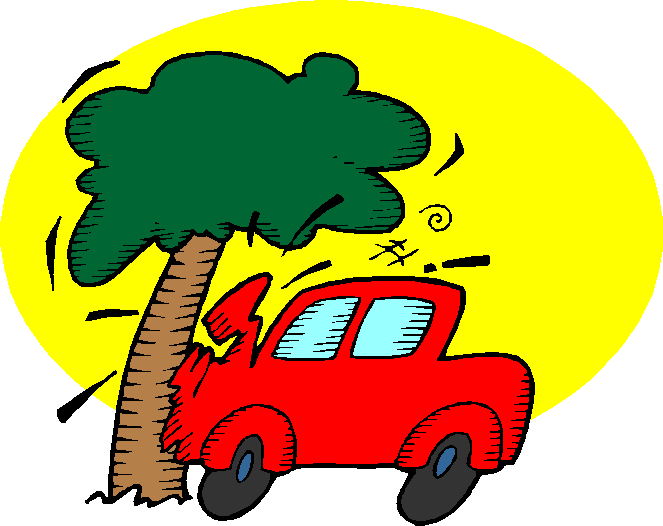
\includegraphics[width=1.75in]{../graphics/a2Homework-img1}
%%  \vspace{\stretch1}
  
\item In a crash test, a car strikes a wall with an average force of 
  \SI{1.23e7}{\newton} [S] over an interval of \SI{21.0}{\milli\second}.
  Calculate the impulse the car exerts on the wall.
  
\item In a crash test similar to the one described in the last problem, another
  car, with the same mass and velocity as the first car, experiences an impulse
  identical to the value you calculated in the last problem. However, the
  second car is designed to crumple more slowly than the first. As a result,
  the duration of the crash is \SI{57.1}{\milli\second}. Determine the average
  force the wall exerted on the second car.
  
\item A \SI{1385}{\kilo\gram} cannon containing a \SI{58.5}{\kilo\gram} cannon
  ball is on wheels. The cannon fires the cannon ball, giving it a velocity of
  \SI{49.8}{\metre\per\second} [N]. What is the initial velocity of the cannon
  the instant after it fires the cannon ball?
 
\item Two amusement park bumper cars are heading directly towards each other.
  The combined mass of car A plus driver is \SI{375}{\kilo\gram} and it is
  moving with a velocity of $+$\SI{1.8}{\metre\per\second}. The combined mass
  of car B plus driver is \SI{422}{\kilo\gram} and it is moving with a velocity
  of \SI{-1.4}{\metre\per\second}. When they collide, they become stuck
  together and continue moving along the same straight line. What is their
  velocity immediately after they collide?

%  \item An \SI{80}{\kilo\gram} astronaut has become detached from the
%  safety line connecting her to the International Space Station. She is
%  \SI{200}{\metre} from the station, and at rest relative to it. She only has
%  4.0 minutes of air remaining. To get herself back, she tosses a
%  \SI{10}{\kilo\gram} tool kit away from the station at
%  \SI{8.0}{\metre\per\second}. Will she make it back in time?
%  \vspace{\stretch1}
%  \newpage
%  
%  \item A \SI{2.0}{\kilo\gram} box is initially moving at
%  $+$\SI{3.0}{\metre\per\second} and is pushed along a horizontal, frictionless
%  surface with a net force $F$ that varies with time according to the following
%  graph:
%  \begin{center}
%    \begin{tikzpicture}[yscale=.14]
%      \foreach\x in {1,...,7} \draw(\x,1)--(\x,-1) node[below]{$\x$};
%      \foreach\y in {-10,-5,...,20}{
%        \draw[thin,gray!50] (7.5,\y)--(-.1,\y) node[left,black]{$\y$};
%      }
%      \draw[axes] (0,0)--(7.5,0) node[right]{$t$ (s)};
%      \draw[axes] (0,-13)--(0,25) node[above]{$F$ (N)};
%      \draw[ultra thick] (0,20)--(1,20)--(3,0)--(4,0)--(5,-10)--(7,-10);
%    \end{tikzpicture}
%  \end{center}
%  \begin{enumerate}[itemsep=3pt]
%    \item In the table below, indicate the momentum change of the box during
%    each second of elapsed time.
%    \begin{center}
%      {\large
%        \begin{tabular}{c|c}
%          Time (s) & Impulse (\si{\newton\second}) \\\hline
%          $0-1$ &\\
%          $1-2$ &\\
%          $2-3$ &\\
%          $3-4$ &\\
%        \end{tabular}
%        \hspace{.7in}
%         \begin{tabular}{c|c}
%          Time (s) & Impulse (\si{\newton\second}) \\\hline
%          $4-5$ &\\
%          $5-6$ &\\
%          $6-7$ &\\
%           & 
%        \end{tabular}
%      }
%    \end{center}
%
%    \item Plot the velocity vs.\ time graph for this motion in the space below.
%    Label all relevant quantities on the $x$ and $y$ axis.
%    \begin{center}
%      \begin{tikzpicture}[scale=.8]
%        \draw[gray!40] grid (7,8);
%        \draw[axes] (0,0)--(0,8.5) node[above]{$v$ (\si{\metre\per\second})};
%        \draw[axes] (0,0)--(7.5,0) node[right]{$t$ (\si\second)};
%      \end{tikzpicture}
%    \end{center}
%    \item At $t=\SI{7.0}\second$, the box collides with a wall and bounces
%    backwards at \SI{6.0}{\metre\per\second}. Given that the box is in contact
%    with the wall for \SI{.20}\second, calculate the average force that the
%    wall exerts on the box.
%
%  \end{enumerate}
%  \newpage
%  
%%  \item A billiard ball of mass \SI{0.155}{\kilo\gram} (``cue ball'') moves
%%  with a velocity of \SI{12.5}{\metre\per\second} towards a stationary billiard
%%  ball (``eight ball'') of identical mass and strikes it with a glancing blow.
%%  The cue ball moves off at an angle of \ang{29.7} clockwise from its original
%%  direction, with a speed of \SI{9.56}{\metre\per\second}.
%%  \begin{enumerate}[itemsep=3pt]
%%    \item What is the velocity of the eight ball?
%%    \item Determine whether the collision was elastic.
%%  \end{enumerate}
  
\item A \SI{1875}{\kilo\gram} car is travelling along a country road when the
  driver sees a deer dart out onto the road. The driver slams on the brakes
  and manages to stop before hitting the deer. The driver of a second car (mass
  \SI{2135}{\kilo\gram}) is driving too close. When the driver realizes that
  the car ahead has stopped, he hits the brakes but is unable to stop. The two
  cars lock together and skid another \SI{4.58}{\metre} along a straight line
  before coming to a stop. If the coefficient of friction between concrete and
  rubber is 0.750, what is the speed of the second car when it hits the stopped
  car?

\item While playing a game of billiards, your \SI{.17}{\kilo\gram} cue ball,
  travelling at \SI{1.9}{\metre\per\second}, glances off a stationary
  \SI{.16}{\kilo\gram} ``eight ball'' so that the eight ball moves off at
  \SI{1.3}{\metre\per\second} at an angle of \ang{32} clockwise from the cue
  ball's original path.
  \begin{enumerate}[itemsep=3pt]
  \item What is the final velocity (both magnitude and direction) of the cue
    ball?
  \item Calculate the total kinetic energy before and after the collision. Is
    the collision elastic?
  \end{enumerate}

%  \item Two blocks are free to slide along the frictionless wooden track
%  shown below. The block of mass $m_1=\SI{4.98}{\kilo\gram}$ is released from
%  the position shown, at height $h=\SI{5.00}\metre$ above the flat part of the
%  track. Protruding from its front end is the north pole of a strong magnet,
%  which repels the north pole of an identical magnet embedded in the back end
%  of the block of mass $m_2=\SI{9.40}{\kilo\gram}$, initially at rest. The two
%  blocks never touch.
%  \begin{center}
%    \begin{tikzpicture}
%      \draw[thick,fill=brown!50] (0,0)--(0,4)--(1,4)--(1,3.5) to[out=270,in=180]
%      (5,.5)--(12,.5)--(12,0)--(0,0);
%      \draw[thick,dashed] (.2,.5)--(5,.5);
%      \draw[thick,dashed] (.2,3.5)--(1,3.5);
%      \draw[<->,thick] (.5,.5)--(.5,3.5) node[midway,fill=brown!50]{$h$};
%      \draw[mass] (5.2,.5) rectangle (5.8,.9) node[right=-1]{$m_2$};
%      \draw[mass] (1,4) rectangle (1.4,3.5)
%      node[right=0]{$m_1$};
%    \end{tikzpicture}
%  \end{center}
%  Calculate:
%  \begin{enumerate}[itemsep=3pt]
%    \item The speed of $m_1$ just before the collision
%    \item The velocities of $m_1$ and $m_2$ after the elastic collision
%    \item The maximum height to which $m_1$ rises after the elastic collision
%  \end{enumerate}
\end{enumerate}


%
%\chapter{Harmonic Motion}
\label{chapter:harmonic-motion}

In Chapter~\ref{chapter:energy}, we studied several oscillatory systems using
the law of conservation of energy, shown in ~\ref{fig:shm-systems}. But it is
clear that the law of conservation of energy does not tell us \emph{why} the
masses oscillate.
\begin{figure}[ht]
  \centering
  \begin{subfigure}{.32\textwidth}
    \centering
    \begin{tikzpicture}[scale=.85]
      \draw[mass] (3,.5) rectangle +(1,1);
      \draw[thick,
        decoration={aspect=.3,segment length=6, amplitude=2.5mm, coil},
        decorate] (0,1)--(3,1);
      \fill[pattern=north east lines] (4.3,0.5)--(4.3,.3)--(-.2,.3)
      --(-.2,2)--(0,2)--(0,.5)--cycle;
      \draw[very thick] (0,2)--(0,.5)--(4.3,.5);
    \end{tikzpicture}
    \caption{Horizontal spring-mass system}
  \end{subfigure}
%    \begin{displaymath}
%      K+U_e=\text{constant}
  %    \end{displaymath}
  \hspace{\stretch1}
  \begin{subfigure}{.32\textwidth}
    \centering
    \begin{tikzpicture}
      \draw[mass] (.7,1.9) rectangle +(.6,.6);
      \draw[thick,
        decoration={aspect=.3,segment length=6, amplitude=2.5mm, coil},
        decorate] (1,5)--(1,2.5); 
      \fill[pattern=north east lines] (0,5) rectangle (2,5.2);
      \draw[very thick] (0,5)--(2,5);
    \end{tikzpicture}
    \caption{Vertical spring-mass system}
%    \begin{displaymath}
%      K+U_e+U_g=\text{constant}
%    \end{displaymath}
  \end{subfigure}
  \hspace{\stretch1}
  \begin{subfigure}{.32\textwidth}
    \centering
    \begin{tikzpicture}
      \fill[pattern=north east lines] (-1,0) rectangle (1,.2);
      \draw[very thick] (-1,0)--(1,0);
      \begin{scope}[rotate=15]
        \draw[thick] (0,0)--(0,-3);% node[midway,right]{$\ell$};
        \shade[ball color=blue] (0,-3) circle (.2);
      \end{scope}
      \draw[dashed,thin] (0,0)--(0,-3);
    \end{tikzpicture}
   \caption{Simple pendulum system}
%    \begin{displaymath}
%      K+U_g=\text{constant}
%    \end{displaymath}
  \end{subfigure}
  \caption{Common examples of harmonic oscillators}
  \label{fig:shm-systems}
\end{figure}

To understand how these systems oscillate, we have to go back to the dynamics
(i.e.\ using free-body diagrams and second law of motion) of such a system,
called a \textbf{harmonic oscillator}. These types of oscillatory motion is
called \textbf{harmonic motion}. Solving these problems generally requires
calculus.

%In Chapter~\ref{chapter:dynamics}, we showed that Hooke's law for ideal springs
%relates the spring force $\bm F_s$ exerted by a compressed or stretched spring
%onto another object to the spring constant (the stiffness of the spring),
%%$k$\footnote{It is the stiffness of the spring, also called \textbf{Hooke's
%%  constant}, \textbf{force constant}, or the \textbf{spring rate} of the
%%spring. It depends on both the geometry of the spring, as well as the material
%%properties of the spring.},
%and the spring's displacement $\bm x$:
%\begin{equation*}
%  \bm F_s=-k\bm x
%\end{equation*}
%In Chapter~\ref{chapter:energy}, was showed when the spring is compressed or
%stretched, the work done by the spring force is equal to the change in the
%elastic potential energy stored in the spring:
%\begin{equation*}
%  W_s=\int^{x_1}_{x_0}F_s\dl x %=\int^{x_1}_{x_0}(-kx)\dl x
%  =-\frac12kx^2\Big|^{x_1}_{x_0}=-\Delta U_s
%  \quad\text{where}\quad
%  U_s=\frac12kx^2
%\end{equation*}
%Because the work done is equal to the negative change in the potential
%energy:
%\begin{equation*}
%  W_s=-\Delta U_s
%\end{equation*}
%the spring force is a conservative force. In spring-mass systems studied in
%Chapter~\ref{chapter:energy}, the total mechanical energy is always conserved
%when there is no friction, drag, or damping forces. However, applying the law of
%conservation of energy does not immediately show us the type of motion in
%spring-mass systems.

\section{Horizontal Spring-Mass System}
Consider the forces acting on a mass connected horizontally to a spring without
friction, drag, and other damping forces, as shown in
Fig.~\ref{fig:horizontal-spring-mass1}. Three forces act on the mass: gravity
$\bm F_g=m\bm g$, normal force $\bm F_n$, and spring force $\bm F_s$.
\begin{figure}[hbt]
  \centering
  \begin{tikzpicture}[scale=1.3]
    \draw[mass] (5,.5) rectangle (6,1.5);
    \draw[thick,decorate,
      decoration={aspect=.4,segment length=8,amplitude=8,coil}] (0,1)--(5,1);
    \fill[pattern=north east lines] (6.5,.5)--(6.5,.3)--(-0.2,.3)
    --(-.2,2)--(0,2)--(0,.5)--cycle;
    \draw[thick] (6.5,.5)--(0,.5)--(0,2);
    \draw[axes] (6.5,1)--+(.8,0) node[right]{$+$};
    \draw[dashed] (3.5,-.5)--+(0,3) node[above]{Unstretched/Equilibrium};
    \draw[vector] (3.5,0)--(5,0) node[midway,below]{$x$};
    \fill[red] (5.5,1) circle (.08);
    \draw[vector,red] (5.5,1)--(5.5,0) node[below]{$\bm F_g$};
    \draw[vector,red] (5.5,1)--(5.5,2) node[above]{$\bm F_n$};
    \draw[vector,red] (5.5,1)--(4.5,1) node[above]{$\bm F_s$};
  \end{tikzpicture}
  \caption{A horizontal spring-mass system with no friction, drag and damping
    forces}
  \label{fig:horizontal-spring-mass1}
\end{figure}
Since there is no vertical motion, $\sum\bm F_\text{vertical}=0$, $\bm F_g$ and
$\bm F_n$ cancel out. The net force is due only to spring force
$\bm F_s=-k\bm x$ in the horizontal direction. This is true when the spring is
in compression, as well as in extension\footnote{It should be obvious that the
spring in Fig.~\ref{fig:horizontal-spring-mass1} is in extension.}. The spring
force is called a \emph{restoring force} because $\bm F_S$ always points
towards the equilibrium position.

Applying second law of motion in the horizontal direction, we can equate the
spring force to mass and horizontal acceleration:
\begin{equation}
  \underbrace{-kx}_{=F_\text{net}=F_s} =m\diff[2]xt
  \label{eq:ode1}
\end{equation}
Eq.~\ref{eq:ode1} is
\emph{second-order ordinary differential equation with constant
coefficients}\footnote{In many math textbooks, Eq.~\ref{eq:ode1} would be
written in standard form:
\begin{equation*}
  \diff[2]xt + \frac kmx=0
\end{equation*}
}. The solution to the equation is a function $x(t)$ where the second time
derivative $\diff[2]xt$ looks like $x$ but with a negative sign. The only
functions that have this property are the sinusoidal functions: $\sin(t)$ and
$\cos(t)$, which means that the motion along the horizontal direction
\emph{must} be periodic. Starting with this general form:
\begin{equation}
  \boxed{
    x(t)=A\cos(\omega t+\theta_0)
  }
  \label{eq:gen-form}
\end{equation}
where $A$ is the amplitude of the oscillation, $\omega$ is the angular
frequency of the motion, called \textbf{natural frequency}, and $\theta_0$ is a
phase constant based on initial condition. We will use the cosine function here
for simplicity. Motion in the form of Eq.~\ref{eq:gen-form} is called the
\textbf{simple harmonic motion}\footnote{This type of periodic motion is also
known as \textbf{oscillatory motion}, \textbf{oscillations},
\textbf{vibrations}.}.

Taking the time derivatives of Eq.~\ref{eq:gen-form} give us expressions for
velocity and acceleration of the mass:
\begin{equation}
  \boxed{
    v(t)=\diff xt=-A\omega\sin(\omega t+\theta_0)
  }
\end{equation}
\begin{equation}
  \boxed{
    a(t)=\diff[2] xt=-A\omega^2\cos(\omega t+\theta_0)=-\omega^2x
  }
\end{equation}
We note that the expression of acceleration is related to position $x(t)$ by
the constant $-\omega^2$. Substituting expressions of $x(t)$ and $a(t)$ back
into Eq.~\ref{eq:ode1}, we find that the ODE is satisfied if the natural
frequency $\omega$ is related to the spring constant and mass by:
\begin{equation}
  \boxed{
    \omega=\sqrt{\frac km}
  }
\end{equation}

\begin{common-question}
  \textbf{When should we use cosine, and when should be use sine?} Both
  functions can be solutions to Eq.~\ref{eq:ode1}, choosing the correct
  function is down to the initial condition (i.e.\ when motion begins at $t=0$.
  If oscillation begins at amplitude $A$ at $t=0$, the cosine function is
  preferred so that we can set $\theta_i=0$:
  \begin{center}
    \begin{tikzpicture}[scale=.9]
      \draw[mass] (4,.5) rectangle +(1,1);
      \draw[thick,
        decoration={aspect=.3,segment length=2mm, amplitude=2.5mm, coil},
        decorate] (0,1)--(4,1);
      \fill[pattern=north east lines] (5.5,.5)--(5.5,.3)--(-.2,.3)
      --(-0.2,1.5)--(0,1.5)--(0,.5)--cycle;
      \draw[very thick] (0,1.5)--(0,.5)--(5.5,.5);
      \draw[vectors] (2.5,1.65)--(4,1.65) node[midway,above]{$x=+A$};
      \draw[dashed,thick] (2.5,.2)--(2.5,2) node[above=0]{equilibrium};
    \end{tikzpicture}
  \end{center}
  If the spring is initially compressed to $x=-A$, use the $-\cos$ function.
  
  Conversely, if the mass is given a ``tap'' in the ($+$) direction at $t=0$ to
  give it an initial velocity of $v=v_\text{max}$, then the sine function is
  preferred. In this case, the oscillator has an initial position of $x=0$ at
  $t=0$.
  \begin{center}
    \begin{tikzpicture}[scale=.95]
      \draw[mass] (2.5,.5) rectangle +(1,1);
      \draw[thick,
        decoration={aspect=.3,segment length=1.3mm, amplitude=2.5mm, coil},
        decorate] (0,1)--(2.5,1);
      \fill[pattern=north east lines] (5.5,.5)--(5.5,.3)--(-.2,.3)
      --(-0.2,1.5)--(0,1.5)--(0,.5)--cycle;
      \draw[very thick] (0,1.5)--(0,.5)--(5.5,.5);
      \draw[vectors] (3,1)--+(1,0) node[right]{$v=v_\text{max}$};
      \draw[dashed,thick] (2.5,.2)--+(0,1.8) node[above=0]{equilibrium};
    \end{tikzpicture}
  \end{center}
  If the sine function is used, we can use the following functions of time
  for the mass's position, velocity and acceleration:
  \begin{align*}
    x(t)&=A\sin(\omega t)\\
    v(t)&=A\omega\cos(\omega t)\\
    a(t)&=-A\omega^2\sin(\omega t)
  \end{align*}
  Mathematically, the two functions only differ by a phase constant of
  $\frac{\pi}2$.
\end{common-question}

%The angular frequency for the simple harmonic oscillator is called the
%\textbf{natural frequency}.
The period ($T$, measured in seconds) and frequency ($f$, measured in Hertz) of
the simple harmonic oscillator are then given by:
\begin{equation}
  \boxed{
    f=\frac\omega{2\pi}=\frac1{2\pi}\sqrt{\frac km}
  }
\end{equation}
\begin{equation}
  \boxed{
    T=\frac1f=2\pi\sqrt{\frac mk}
  }
\end{equation}
It should be clear that angular frequency ($\omega$), frequency ($f$), and
period ($T$) are all independent of amplitude $A$.


%\begin{frame}{Displacement, Velocity and Acceleration}
%    \begin{align*}
%      x(t)&=A\cos(\omega_0 t-\phi)\\
%      v(t)&=-A\omega_0\sin(\omega_0 t-\phi)\\
%      a(t)&=-A\omega_0^2\cos(\omega_0 t-\phi)=-\omega_0^2x
%    \end{align*}
%
%    \column{.6\textwidth}
%    \begin{tikzpicture}[yscale=.5]
%      \draw[axes] (0,-2)--(0,2) node[left]{$x$};
%      \draw[axes] (-1,0)--(8,0) node[right]{$t$};
%      \draw[functions,smooth,samples=80,domain=0:7.5]
%      plot(\x,{1.5*cos(90*\x)});
%      
%      \draw[axes] (0,-7)--(0,-3)  node[left]{$v$};
%      \draw[axes] (-1,-5)--(8,-5) node[right]{$t$};
%      \draw[blue,very thick,smooth,samples=80,domain=0:7.5]
%      plot(\x,{-1.5*sin(90*\x)-5});
%      
%      \draw[axes] (0,-12)--(0,-8)  node[left]{$a$};
%      \draw[axes] (-1,-10)--(8,-10) node[right]{$t$};
%      \draw[violet,very thick,smooth,samples=80,domain=0:7.5]
%      plot(\x,{-1.5*cos(90*\x)-10});
%    \end{tikzpicture}

\begin{common-question}
  \textbf{Is $\omega$ the same angular velocity term from circular motion?}
  Yes, it most certainly is. In fact, the simple harmonic motion is the
  projection of a uniform circular motion onto an axis. For a uniform circular
  motion with a radius $r$, the object's angular position is given by
  $\theta(t)=\omega t+\theta_i$, then
  $x(t)=r\cos(\theta)=r\cos(\omega t+\theta_i)$ which is the same form as
  Eq.~\ref{eq:ode1}. The radius $r$ of the circular motion is the amplitude
  $A$ of the harmonic motion. We can also project on to the $y$ axis as well,
  and get $y(t)=r\sin(\omega t +\theta_i)$.
  \begin{center}
    \begin{tikzpicture}[scale=.7]
      \draw[axes] (-3,0)--(3,0) node[right]{$x$};
      \draw[axes] (0,-3)--(0,3) node[above]{$y$};
      \draw circle (2.5);
      \begin{scope}[rotate=38]
        \draw[vector] (0,0)--(2.45,0) node[midway,above]{$r$};
        \draw[mass] (2.5,0) circle (.1);
      \end{scope}
      \draw[axes] (1.5,0) arc (0:38:1.5) node[pos=.55,right]{$\theta(t)$};
      \draw[vector] (0,0)--({2.5*cos(38)},0) node[midway,below]{$x(t)$};
      \draw[dashed] ({2.5*cos(38)},0)--({2.5*cos(38)},{2.5*sin(38)});
    \end{tikzpicture}
  \end{center}
\end{common-question}


%\begin{remark}%sidenote}
%  Generally in calculus classes, you would be taught that the solution to any
%  ODE is the linear combination of \emph{all} possible solutions, i.e.:
%  \begin{equation*}
%    x(t)=c_1\cos(\omega t)+c_2\sin(\omega t)
%  \end{equation*}
%  Where $c_1$ and $c_2$ are coefficients based on initial position $x_0=x(0)$
%  and initial velocity $v_0=v(0)$. Trigonometric identities can be used to
%  Eq.~\ref{eq:gen-form} is identical to the form of solution above:
%  \begin{align*}
%    x(t)&=A\cos(\omega t+\phi)\\
%    &=A\left[\cos(\omega t)\cos(\phi)+\sin(\omega t)\sin(\phi)\right]\\
%    &=\underbrace{A\cos(\phi)}_{c_1}\cos(\omega t)
%    +\underbrace{A\sin(\phi)}_{c_2}\sin(\omega t)
%  \end{align*}
%  From an even broader discussions on mathematics, which is not part of the
%  discussion in physics, the solution to any ODE is a
%  \emph{linear combination} of all the possible solutions. And all the
%  possible solutions are, in fact, functions that are \emph{orthogonal} to
%  each other. In essence, the orthogonal functions are treated as basis
%  vectors (much like the $x$ axis is orthogonal to the $y$ axis) and
%  the solution is a vector in this functional space.
%\end{remark}%sidenote}
%
%\begin{remark}%sidenote}
%  Another function that we can try is the exponential function, where its
%  derivatives is related to the function itself:
%  \begin{align*}
%    x(t) &=Ae^{\omega t}\\
%    \diff xt &=A\omega e^{\omega t}\\
%    \diff[2] xt &=A\omega^2 e^{\omega t}=\omega^2x\label{eq:2nd-derivative}
%  \end{align*}
%  It is clear that the second derivative (Eq.~\ref{eq:2nd-derivative}) does
%  not have the negative sign that we need. However, if the exponential
%  function is \emph{imaginary}, i.e.:
%  \begin{equation*}
%    x(t)=Ae^{i\omega t}
%  \end{equation*}
%  Then the second derivative \emph{does} in fact have the negative sign:
%  \begin{align*}
%    \dot x&=iA\omega e^{i\omega t}\\
%    \ddot x&=i^2A\omega^2 e^{i\omega t}=-\omega^2 e^{i\omega t}=-\omega^2x
%  \end{align*}
%  This should not come as a surprise, since the complex exponential function
%  and the sinusoidal functions are related:
%  \begin{equation*}
%    e^{i\omega t}=\cos(\omega t)+i\sin(\omega t)
%  \end{equation*}
%\end{remark}%sidenote}

\section{Vertical Spring-Mass System}

For vertical spring-mass systems, shown in
Fig.~\ref{fig:vertical-spring-mass}), we must also consider the gravitational
force $\bm F_g=m\bm g$ which acts along the direction of motion. In this case,
the presence of gravity shifts the equilibrium position to a distance $B$ away
from the unstretched position of the spring.
\begin{figure}[ht]
  \centering
  \begin{tikzpicture}[scale=1.3]
    \draw[mass] (.7,1.7) rectangle (1.3,2.3);
    \draw[thick,
      decoration={aspect=.3,segment length=2mm, amplitude=2.5mm, coil},
      decorate] (1,5)--(1,2.5); 
    \fill[pattern=north east lines] (0,5) rectangle (2,5.2);
    \draw[very thick] (0,5)--(2,5);
    \draw[vector,red] (1,2)--(1,1.2) node[right]{$\bm F_g$};
    \draw[vector,red] (1,2)--(1,2.8) node[right]{$\bm F_s$};
    \fill[red] (1,2) circle (.05);
    \draw[axes] (1,1)--(1,.5) node[below]{$+$};
    \draw[vector] (.3,4)--(.3,2.3) node[midway,left]{$x$};
    \draw[vector] (1.7,4)--(1.7,3.5) node[midway,right]{$B$};
    \begin{scope}[thick,dashed]
      \draw (0,4)--(2,4) node[right]{\scriptsize unstretched};
      \draw (0,3.5)--(2,3.5) node[right]{\scriptsize equilibrium};
    \end{scope}
  \end{tikzpicture}
  \caption{A vertical spring-mass system with no friction and damping force}
  \label{fig:vertical-spring-mass}
\end{figure}
Using the downward direction as the
positive direction of motion, the second law of motion becomes:
\begin{equation}
  mg-kx=m\diff[2]xt
  %\label{eq:ode2}
\end{equation}
Since $F_g$ is constant, the only change is the addition of a constant $B$
in the expression of $x(t)$:
\begin{equation}
  x(t) = A\cos(\omega t+\phi) + B\\
  \label{eq:ode1a}
\end{equation}
%  \begin{columns}
%    \column{.3\textwidth}
%    \begin{tikzpicture}[scale=1.3]
%      \draw[mass] (.7,1.7) rectangle (1.3,2.3);
%      \draw[thick,
%        decoration={aspect=0.3,segment length=2mm, amplitude=2.5mm, coil},
%        decorate] (1,5)--(1,2.5); 
%      \fill[pattern=north east lines] (0,5) rectangle (2,5.2);
%      \draw[very thick] (0,5)--(2,5);
%      \draw[vector,red] (1,2)--(1,1.2) node[right]{$\bm F_g$};
%      \draw[vector,red] (1,2)--(1,2.8) node[right]{$\bm F_s$};
%      \fill[red] (1,2) circle (.05);
%      \draw[axes] (1,1)--(1,.5) node[below]{$+$};
%      \draw[vector] (.3,4)--(.3,2.3) node[midway,left]{$x$};
%      \draw[vector] (1.7,4)--(1.7,3.5) node[midway,right]{$B$};
%      \begin{scope}[thick,dashed]
%        \draw (0,4)--(2,4) node[right]{\scriptsize unstretched};
%        \draw (0,3.5)--(2,3.5) node[right]{\scriptsize equilibrium};
%      \end{scope}
%    \end{tikzpicture}

The constant $B$ is the shift of the equilibrium position from the unstretched
position. It is found by equating $F_s=F_g$ and solving for the spring extension
at $x=B$:
\begin{equation}
  B=\frac{mg}k
\end{equation}
%is found by substituting $x$ and $\ddot x$ into the ODE. It is the stretch
%of the spring due to its own weight:
Since $B$ is a constant, velocity and acceleration as functions of time are
unchanged from the horizontal spring-mass case:
\begin{align*}
  v(t) &= -A\omega\sin(\omega t+\phi)\\
  a(t) &= -A\omega^2\cos(\omega t+\phi)
\end{align*}
Angular frequency (natural frequency) also remains the same as the horizontal
spring-mass system:
\begin{equation*}
  \omega=\sqrt{\frac km}
\end{equation*}

%\subsection{Conservation of Energy in a Spring-Mass System}
%In the spring-mass systems, if there are no frictional losses, then the only
%forces doing work are the spring force (horizontal and vertical) and gravity
%(vertical). Both forces are \emph{conservative}, therefore the total mechanical
%energy is conserved:
%\begin{equation}
%  K + U_s + U_g = K' + U_s' + U_g'
%\end{equation}
%For the horizontal spring-mass system, the total energy of the simple harmonic
%oscillator is:
%\begin{equation}
%  \boxed{E_T=\frac12kA^2}
%\end{equation}

\begin{example}
  A mass suspended from a spring is oscillating up and down. Consider the
  following two statements:
  \begin{enumerate}[nosep]
  \item At some point during the oscillation, the mass has zero velocity but
    it is accelerating
  \item At some point during the oscillation, the mass has zero velocity and
    non-zero acceleration.
  \end{enumerate}
  \begin{enumerate}[nosep]
  \item Both occur at some time during the oscillation
  \item Neither occurs during the oscillation
  \item Only (1) occurs
  \item Only (2) occurs
  \end{enumerate}
\end{example}

\begin{example}
  An object of mass \SI5{\kilo\gram} hangs from a spring and oscillates with a
  period of \SI{.5}\second. By how much will the equilibrium length of the
  spring be shortened when the object is removed.
  %\begin{enumerate}[nosep]
  %\item\SI{.75}{\centi\metre}
  %\item\SI{1.5}{\centi\metre}
  %\item\SI{3.1}{\centi\metre}
  %\item\SI{6.2}{\centi\metre}
  %\end{enumerate}
\end{example}



\section{Simple Pendulum}
Aside from spring-mass systems, simple pendulums also exhibit the same kind
of oscillatory motion that we find in spring-mass systems. In the simplest
case, two forces act on the mass: weight $\bm F_g$ and tension $\bm F_T$, as
shown in Fig.~\ref{fig:pendulum1}.
\begin{figure}[ht]
  \centering 
  \begin{tikzpicture}
    \fill[pattern=north east lines] (-1,0) rectangle (1,0.2);
    \draw[thick] (-1,0)--(1,0);
    \begin{scope}[rotate=20]
      \draw[thick] (0,0)--(0,-5) node[midway,right]{$\ell$};
      \shade[ball color=red] (0,-5) circle (.2) node[below right]{$m$};
      \draw[vector,red,dotted] (0,-5)--(-1.5*sin{20},-5)
      node[left,fill=yellow!10]{$mg\sin\theta$};
      \draw[vector,red] (0,-5)--(0,-3) node[left]{$\bm F_T$};
      \draw[vector,red,rotate around={-20:(0,-5)}] (0,-5)--(0,-6.5)
      node[below]{$\bm F_g$};
    \end{scope}
    \draw[axes] (0,-2) arc (270:290:2) node[midway,below]{$\theta$};
    \draw[dashed] (0,0)--(0,-5);
    \draw[dashed] (0,-5) arc (270:295:5);
    \draw[dashed] (0,-5) arc (270:255:5);
  \end{tikzpicture}
  \caption{A simple pendulum deflected by an angle $\theta$}
  \label{fig:pendulum1}
\end{figure}
We have already shown in Chapter~\ref{chapter:circ-motion} that when the mass
is deflected by an angle $\theta$, the tangential force is
$F_t=mg\sin\theta$. As we are interested in the pendulum's motion in the
angular direction, there is no need to worry about the radial direction; it
does not have to do with the restoring force.

Substitute $F_t$ into the second law of motion, and cancelling $m$:
\begin{equation}
  F_t=ma_t\quad\rightarrow\quad
  -mg\sin\theta=m\ell\diff[2]{\theta}t
  \quad\rightarrow\quad
  -g\sin\theta=\ell\diff[2]{\theta}t
\end{equation}
Solving this ODE is very difficult because of the $\sin\theta$ term. However,
we can simplify the problem by using the Taylor series expansion of the sine
function:
\begin{equation}
  \sin\theta
  =\theta-\frac{\theta^3}{3!}+\frac{\theta^5}{5!}-\frac{\theta^7}{7!}+\cdots
\end{equation}
For small angles of $\theta$, we can use the \emph{small-angle approximation},
where
\begin{equation}
  \sin\theta\approx\theta
\end{equation}

%    \centering
%    \begin{tikzpicture}
%      \fill[pattern=north east lines] (-1,0) rectangle (1,0.2);
%      \draw[thick] (-1,0)--(1,0);
%      \begin{scope}[rotate=20]
%        \draw[thick] (0,0)--(0,-5) node[midway,right]{$\ell$};
%        \shade[ball color=red] (0,-5) circle (.2) node[below right]{$m$};
%      \end{scope}
%      \draw[axes] (0,-2) arc (270:290:2) node[midway,below]{$\theta$};
%      \draw[dashed] (0,0)--(0,-5);
%      \draw[dashed] (0,-5) arc (270:295:5);
%      \draw[dashed] (0,-5) arc (270:255:5);
%    \end{tikzpicture}

and the ODE reduces to the same form as the spring-mass system
\begin{equation}
  \diff[2]{\theta}t + \frac g\ell\theta=0
\end{equation}
The solution for $\theta(t)$ is a sinusoidal function, like the spring-mass
system:
\begin{equation}
  \boxed{\theta(t)=\theta_\text{max}\cos(\omega t-\phi)}
\end{equation}
where $\theta_\text{max}$ is the maximum deflection (amplitude), and $\phi$ is a
phase shift based on the initial condition of the pendulum. (If the oscillation
begins at amplitude, then $\phi=0$) The natural frequency of the oscillation
$\omega$ is given by:
\begin{equation}   
  \boxed{
    \omega=\sqrt{\frac g\ell}
  }
\end{equation}

\begin{common-question}
  \textbf{How small is a ``small angle''?} What constitutes a small angle
  depends on what tolerance (i.e.\ the number of significant figures) is needed
  in the answer. When we plot the difference between $y=\sin\theta$, and our
  approximation $y=\theta$, we can see that both functions agree well near
  $\theta=0$. However, $\sin\theta$ levels off towards $\theta=\frac\pi2$ and
  the linear function (obviously) does not. We can calceulate the percentage
  error:
  \begin{equation*}
    \text{\% Error}=\frac{\theta-\sin\theta}{\sin\theta}\times\SI{100}\percent
  \end{equation*}
  which shown on the right. For a \SI1{\percent} error, the angle of deflection
  should be kept to less than \SI4\degree.
  \begin{center}
    \begin{tikzpicture}
      \begin{axis}[
          width=2.3in,
          xmin=0,xmax=pi/2,
          ymin=0,ymax=pi/2,
          %xlabel=$\theta$ (radian),
          xtick={0,pi/8,pi/4,3*pi/8,pi/2},
          xticklabels={
            0,$\dfrac\pi8$,$\dfrac\pi4$,$\dfrac{3\pi}8$,$\dfrac\pi2$
          },
          grid = both,
          legend pos=north west,
        ]
        \addplot[
          color=blue,
          domain=0:pi/2,
          samples=40,
          style={thick}]{sin(x*180/pi)};
        \addlegendentry{$\sin\theta$}
        \addplot[
          color=red,
          domain=0:pi/2,
          samples=40,
          thick]{x};
        \addlegendentry{$\theta$}
      \end{axis}
    \end{tikzpicture}
    \begin{tikzpicture}
      \begin{axis}[
          width=2.3in,
          ylabel=\% Error,
          xmin=0,xmax=pi/2,
          ymin=0,ymax=60,
          %xlabel=$\theta$ (radian),
          xtick={0,pi/8,pi/4,3*pi/8,pi/2},
          xticklabels={
            0,$\dfrac\pi8$,$\dfrac\pi4$,$\dfrac{3\pi}8$,$\dfrac\pi2$
          },
          ytick={0,10,...,60},
          legend pos=north west,
          grid = both,
        ]
        \addplot[
          color=violet,
          domain=0:pi/2,
          samples=40,
          style=thick
        ]{abs(sin(x*180/pi)-x)/sin(x*180/pi)*100};
      \end{axis}
    \end{tikzpicture}
  \end{center}
\end{common-question}

\begin{example}
  A simple pendulum consists of a mass $m$ attached to a light string of length
  $\ell$. If the system is oscillating through small angles, which of the
  following is true?
  \begin{enumerate}[nosep]
  \item The frequency is independent of the acceleration due to gravity, $g$.
  \item The period depends on the amplitude of the oscillation.
  \item The period is independent of the mass $m$.
  \item The period is independent of the length $\ell$.
  \end{enumerate}
\end{example}

\begin{example}
  A bucket full of water is attached to a rope and allowed to swing back and
  forth as a pendulum from a fixed support. The bucket has a hole in its
  bottom that allows water to leak out. How does the period of motion change of
  the bucket with the loss of water?
  \begin{enumerate}[nosep]
  \item The period does not change.
  \item The period continuously decreases.
  \item The period continuously increases.
  \item The period increases to some maximum and then decreases again.
  \end{enumerate}
\end{example}

\begin{example}
  A little girl is playing with a toy pendulum while riding in an elevator.
  Being an astute and educated young lass, she notes that the period of the
  pendulum is $T=\SI{.5}\second$. Suddenly the cables supporting the elevator
  break and all  of the brakes and safety features fail simultaneously. The
  elevator plunges into free fall. The young girl is astonished to discover
  that the pendulum has:
  \begin{enumerate}[nosep]
  \item continued oscillating with a period of \SI{.5}\second.
  \item stopped oscillating entirely.
  \item decreased its rate of oscillation to have a longer period.
  \item increased its rate of oscillation to have a lesser period.
  \end{enumerate}
\end{example}



\section{Damped Oscillator}
In reality, there are friction, or drag, or other damping forces present in the
spring-mass system, represented schematically by the shock absorber, as shown
in Fig.~\ref{fig:damping1}.
\begin{figure}[ht]
  \centering
  \begin{tikzpicture}[scale=1.3]
    \draw[gray,mass] (3,.5) rectangle (4,1.5);
    \draw[thick,draw=gray,decorate,
      decoration={aspect=.4,segment length=5,amplitude=8,coil}] (0,1)--(3,1);
    \fill[gray,pattern=north east lines] (-.2,2)--(-.2,.3)--(6.7,.3)--(6.7,2)
    --(6.5,2)--(6.5,.5)--(0,.5)--(0,2)--cycle;
    \draw[gray,thick] (0,2)--(0,.5)--(6.5,.5)--(6.5,2);
    \draw[axes] (7.25,1)--(8,1) node[right]{$x$};
    \fill[blue!20!white] (5,.8) rectangle (6,1.2);
    \draw[very thick] (4,1)--(5,1);
    \draw[very thick] (5,.8)--(5,1.2);
    \draw[very thick] (4.9,1.2)--(6,1.2)--(6,.8)--(4.9,.8);
    \draw[very thick] (6,1)--(6.5,1);
    \begin{scope}[vector,red]
      \draw (3.5,1)--(3.5,0) node[right]{$\bm F_g$};
      \draw (3.5,1)--(3.5,2) node[right]{$\bm F_n$};
      \draw (3.5,1)--(2.5,1) node[above]{$\bm F_s$};
      \draw (3.5,1)--(4.5,1) node[above]{$\bm F_D$};
    \end{scope}
    \fill[red] (3.5,1) circle (.075);
  \end{tikzpicture}
  \caption{A horizontal spring-mass system with a damping force}
  \label{fig:damping1}
\end{figure}

The damping force is typically related to velocity, but acting the opposite
direction:
\begin{equation}
  \bm F_D=-b\bm v^n
\end{equation}
where $b$ is a positive constant called the \textbf{damping factor}. We
generally use $n=1$ to approximate a mixture of viscous effects.\footnote{Note
that for kinetic friction, $n=0$, for a shock absorber $n=1$, while aerodynamic
drag, $n=2$. Of course our choice of using $n=1$ will not be entirely correct
for every problem, but it is \emph{sufficiently} accurate for a wide range of
situations.} With the addition of the damping force, the differential equation
for the \textbf{damped oscillator} is obtained again by applying second law of
motion, this time with the additional term from the damping force, highlighted
in red:
\begin{align}
  \sum F = {\color{blue}F_s} + {\color{red}F_D} &= m{\color{orange}a}\nonumber\\
  -{\color{blue}kx}-{\color{red}b\diff xt} &= m{\color{orange}\diff[2]xt}
\end{align}
The equation can be arranged into standard form:
\begin{equation}  
  \diff[2]xt+\frac bm\diff xt+\frac kmx=0
  \label{eq:ode2}
\end{equation}
The solution to Eq.~\ref{eq:ode2} is still relatively straightforward, although
not as straightforward as Eq.~\ref{eq:ode1}. The solution has both an
exponential decay term and a sinusoidal (oscillatory) term:
\begin{equation}
  \boxed{
    x(t)=
    \underbrace{A_0 e^{-\frac b{2m}t}}_\text{amplitude $A(t)$}\cos(\omega t+\phi)
  }
  \label{eq:damped-solution}
\end{equation}
where $A_0$ is the initial amplitude of the damped oscillator. This motion is
called a \textbf{damped harmonic motion}.
Unlike simple harmonic motion, the motion of the damped oscillator is not
strictly periodic\footnote{Let's call it \emph{quasi}-periodic.}. The natural
frequency $\omega'$ for the damped oscillator shifted from the undamped case
$\omega$ based on the damping factor $b$:
\begin{equation}
  \boxed{
    \omega'=\sqrt{\omega^2-\left(\frac b{2m}\right)^2}
  }\quad\text{where}\quad
  \omega=\sqrt{\frac km}
  \label{damping1}
\end{equation}
Note that $\omega'<\omega$ (natural frequency decreases) because of the
damping factor $b$.

\textbf{Critical damping} occurs when the damped natural frequency $\omega'$ is
zero, which we can calculate by setting $\omega'=0$ in Eq.~\ref{damping1}, and
solving for the resulting damping constant, which is called the \textbf{critical
  damping constant} $b_c$:
\begin{equation}
  \sqrt{\omega^2-\left(\frac{b_c}{2m}\right)^2}=0
  \quad\longrightarrow\quad
  \boxed{
    b_c=2m\omega=2\sqrt{km}
  }
\end{equation}
A critically damped system returns to its equilibrium position in the shortest
time with \emph{no} oscillation. Critical or near-critical damping is desired
in many engineering designs (e.g.\ shock absorbers on car suspensions). When
$b>b_c$, the system is \textbf{over-damped}.

%\begin{figure}[ht]
%  \centering
%  \pic{.65}{harmonicMotion/oscda8}%\\
%  %\textbf{Better replace this with my own diagram for later}
%\end{figure}



%\subsection{Energy in a Damped System}
%The non-conservative damping force dissipates energy from the oscillator at
%a rate of:
%\begin{equation}
%  P=\diff Et=\bm F_D\cdot\bm v=-bv^2
%\end{equation}
%As velocity relate to energy by: $(v_{av})^2=E/m$, power dissipation is a
%first-order linear ODE:
%\begin{equation}
%  \diff Et=-\frac bmE
%\end{equation}
%The solution to the ODE shows the total amount of energy decreases
%exponentially with time:
%\begin{equation}
%  E(t)=E_0e^{-\frac bmt} %=E_0e^{-\frac{t}{\tau}}
%\end{equation}

\section{Driven Oscillators}
To keep a damped system going, energy must be added into the system. Assuming
that the system is subjected to an external forcing function $F_a(t)$, as shown
in Fig.~\ref{fig:driven1}, that is harmonic with time, with a driving frequency
of $\omega_a$:
\begin{equation}
  \boxed{
    F_a=F\cos(\omega_at)
  }
\end{equation}
In general, the driving frequency $\omega_a$ is unrelated to the undamped
natural frequency $\omega$ or the damped natural frequency $\omega'$.
\begin{figure}[t]
  \centering
  \begin{tikzpicture}[scale=1.3]
    \draw[gray,mass] (3,.5) rectangle (4,1.5);
    \draw[thick,gray,decorate,
      decoration={aspect=.4,segment length=6,amplitude=8,coil}] (0,1)--(3,1);
    \fill[gray,pattern=north east lines] (-.2,2)--(-.2,.3)--(6.7,.3)--(6.7,2)
    --(6.5,2)--(6.5,.5)--(0,.5)--(0,2)--cycle;
    \draw[gray,thick] (0,2)--(0,.5)--(6.5,.5)--(6.5,2);
    \draw[fill=blue!10] (4.9,.8) rectangle (5.5,1.2);
    \draw[very thick,gray] (4,1)--(4.9,1);
    \draw[very thick,gray] (4.9,.8)--(4.9,1.2);
    \draw[very thick,gray] (4.8,1.2)--(5.5,1.2)--(5.5,.8)--(4.8,.8);
    \draw[very thick,gray] (5.5,1)--(6.5,1);
    \begin{scope}[vector,red]
      \draw (3.5,1)--(3.5,0) node[right]{$\bm F_g$};
      \draw (3.5,1)--(3.5,2) node[right]{$\bm F_n$};
      \draw (3.5,1)--(2.5,1) node[above]{$\bm F_s$};
      \draw (3.5,.95)--(2,.95) node[below]{$\bm F_a$};
      \draw (3.5,1)--(4.5,1) node[below]{$\bm F_D$};
    \end{scope}
    \fill[red] (3.5,1) circle (.075);
  \end{tikzpicture}
  \caption{A horizontal spring-mass system with a damping force and an external
    driving force.}
  \label{fig:driven1}
\end{figure}
Again, the second-order ordinary differential equation is obtained by
applying the second law of motion:
\begin{equation}
  \sum F=
  \underbrace{-kx}_{F_s}\underbrace{-bv}_{F_D}+
  \underbrace{F\cos(\omega_at)}_{F_a}=ma
\end{equation}
Rearranging the terms gives a similar ODE to the damped case: the only
difference between Eq.~\ref{eq:ode2} and the current case is the additional
forcing function term on the right-hand side. This is a much more
difficult problem in calculus, but nevertheless still a standard problem.
In standard form:
\begin{equation}
  m\diff[2]xt + b\diff xt+kx=F\cos(\omega_a t)
  \label{eq:ode3}
\end{equation}
The solution to Eq.~\ref{eq:ode3} contains:
\begin{itemize}[nosep,leftmargin=15pt]
\item a \textbf{transient solution} that is obtained by by setting $F_a=0$.
  Essentially this is the solution to the damped harmonic motion case in
  Eq.~\ref{eq:ode2}, and the solution is given in Eq.~\ref{eq:damped-solution}.
  The solution depends on the initial condition, and regardless of the damping
  factor $b$, the solution will become negligible over time because of
  exponential decay.

\item a \textbf{steady-state solution} which does not depend on the initial
  condition, only on the forcing function $\bm F_a$. Solving for the
  steady-state solution will be left as a difficult calculus
  exercise\footnote{This is usually taught in a 2nd-year university level ODE
  course}
\end{itemize}
The steady-state solution is a harmonic motion at the driving frequency
$\omega_a$ of the external force:
\begin{equation}
  \boxed{x(t)=A\cos(\omega_a t+\phi)}
  \label{eq:gen-solution3}
\end{equation}
(For those who are interested, Appendix X shows how the steady-state solution
is derived.) The amplitude of the oscillation $A$ depends on the driving
frequency $\omega_a$ of the forcing function:
\begin{equation}
  \boxed{
    A=\frac F{\sqrt{m^2(\omega^2-\omega_a^2)^2+b^2\omega_a^2}}
  }
  \label{eq:amplitude1}
\end{equation}
%And the phase contant is given by:
%\begin{equation}
%  \tan\phi=\frac{b\omega_a}{m(\omega^2-\omega_a^2)}
%\end{equation}
%
%\begin{frame}{Amplitude Response to External Driving Force}
%The amplitude of the driven oscillation is given by:
%\begin{equation}
%  A=\frac F{\sqrt{m^2(\omega^2-\omega_a^2)^2+b^2\omega_a^2}}
%\end{equation}
Maximum amplitude $A$ occurs when the denominator in Eq.~\ref{eq:amplitude1} is
minimized, i.e.\ when the derivative with respect to external frequency
$\omega_a$ is 0:
\begin{equation}
  \diff{}{\omega_a}\left[m^2(\omega^2-\omega_a^2)^2+b^2\omega_a^2\right]=0
\end{equation}
Taking the derivative and solving for $\omega_a$, we find that maximum
amplitude $A_\text{max}$ occurs when the driving frequency is
\emph{approximately} equal to the damped natural frequency, i.e.\
$\omega_a\approx\omega'$.
\begin{equation}
  \omega_a=\sqrt{\omega^2-\frac{b^2}{2m^2}}\approx\omega'
\end{equation}
(Note that the terms inside the square root is \emph{not} the same as in
Eq.~\ref{damping1}!) %In other words, the driving frequency $\omega_a$ at
%maximum amplitude occurs at a frequency that is very close to (albeit slightly
%different from) the natural frequency of the damped system.

\begin{figure}[ht]
  \centering
  \begin{tikzpicture}
    \begin{axis}[
        width=3.3in,
        xmin=0,xmax=3, xlabel=Driving Frequency ($\omega_a$),
        xtick={0,1,2,3}, xticklabels={0,$\omega$,$2\omega$,$3\omega$},
        ymin=0,ymax=6, ylabel=Relative Amplitude ($A$),
        ytick={0,1,2,3,4,5,6}
      ]
      \addplot[
        color=red!25,
        samples=50,
        domain=0:3,
        very thick]{1/sqrt((1-x^2)^2+x^2)};
      \addlegendentry{$\frac b{2m}=\frac12\omega$}
      \addplot[
        color=red!50,
        samples=80,
        domain=0:3,
        very thick]{1/sqrt((1-x^2)^2+x^2/4)};
      \addlegendentry{$\frac b{2m}=\frac14\omega$}
      \addplot[
        color=red!75,
        samples=250,
        domain=0:3,
        very thick]{1/sqrt((1-x^2)^2+x^2/16)};
      \addlegendentry{$\frac b{2m}=\frac18\omega$}
      \addplot[
        color=red,
        samples=400,
        domain=0:3,
        very thick]{1/sqrt((1-x^2)^2+x^2/32)};
      \addlegendentry{$\frac b{2m}=\frac1{16}\omega$}
    \end{axis}
  \end{tikzpicture}
  \caption{Amplitude response to the driving frequency $\omega_a$.}
  \label{fig:amp-response}
\end{figure}
Plotting amplitude $A$ as a function of driving frequency $\omega_a$ shows
that, for a lightly damped system (i.e.\ small $b$), resonance response is
highest when $\omega_a\approx\omega\approx\omega$, and that smaller the
damping constant $b$, the higher and narrower the peak is.

The phase constant $\phi$ in Eq.\ref{eq:gen-solution3} also depends on the
driving frequency $\omega_a$.
\begin{equation}
  \boxed{\tan\phi=\frac{b\omega_a}{m(\omega^2-\omega_a^2)}}
\end{equation}
When $\omega_a=\omega$ is substituted into the phase shift expression, the
right-hand side becomes undefined. From this, we obtain a phase shift of
$\phi=\pi/2$. Taking derivative of $x(t)$ for velocity $v(t)$, and
substituting $\phi=\pi/2$:
\begin{equation}
  v(t)=\dot x
  =-A\omega_a\sin(\omega_a t-\frac{\pi}2)
  =A\omega_a\cos(\omega_a t)
\end{equation}
At resonance, the object is always moving in the same direction as the
driving force:
\begin{align*}
  v(t)&=A\omega_a\cos(\omega_a t)\\
  F_a(t)&=F\cos(\omega_a t)
\end{align*}
This also makes sense from a work-energy perspective, because now the
external force is doing positive work to the system.

\textbf{Resonance} is caused by in-phase excitation near the natural
frequency. This means that the frequency of the driving force is
\emph{approximately} equal to the natural frequency of the damped oscillator:
\begin{equation}
  \omega_a=\sqrt{\omega^2-\frac{b^2}{2m^2}}
  \quad\text{where}\quad\omega=\sqrt{\frac km}
\end{equation}
For a lightly damped system, $\omega_a\approx\omega\approx\omega$. Also, the
driving force follows the motion of the oscillator.

%\section*{Problems}

\begin{enumerate}
%  \question A mass is attached to a spring and allowed to oscillate vertically.
%  Which of the following would \emph{not} change the period to the oscillation?
%  \begin{choices}
%    \choice Double the mass and double the spring constant
%    \choice Double the amplitude of vibration and the double the mass
%    \choice Double the gravitational field strength $g$ and double the mass
%    \choice Double the gravitational field strength $g$ and double the spring
%    constant
%    \choice Double the gravitational field strength $g$ and quadruple the mass
%  \end{choices}
%
%  \question A particle oscillated with simple harmonic motion with no damping.
%  Which of the following statements about the acceleration of the particle is
%  true?
%  \begin{choices}
%    \choice It has a value of \SI{9.8}{\metre\per\second\squared} when the
%    oscillation is vertical
%    \choice It is zero when the spring is minimum
%    \choice It is proportional to the frequency
%    \choice It is zero throughout the oscillation
%    \choice It is zero when the speed is maximum
%  \end{choices}
%
%  \question At what position does the mass attached to a spring in simple
%  harmonic motion have the greatest magnitude of acceleration? ($A$ is
%  amplitude)
%  \begin{choices}
%    \choice $-A$
%    \choice $-A/2$
%    \choice $0$
%    \choice $A/2$
%    \choice $A/4$
%  \end{choices}
%
%  \item A spring mass system oscillated up and down on Earth. When is the
%  kinetic energy the greatest?
%  \begin{choices}
%    \choice When it is passing through equilibrium
%    \choice At the top of its motion
%    \choice At the bottom of its motion
%    \choice When its gravitational potential energy is the greatest
%    \choice When its elastic energy is the greatest
%  \end{choices}
%  
%  \item An object with a mass $M$ is suspended from an elastic spring with a
%  spring constant $k$. The object oscillates with period $T$ on the surface of
%  Earth. If the oscillating system is moved to the surface of Moon, how it will
%  change the period of oscillations? Acceleration due to gravity on moon is
%  aproximately $\dfrac16 g_\text{Earth}$.
%  \begin{choices}
%    \choice The period is increased by factor of approximately $\sqrt6$
%    \choice The period is increased by factor of approximately 6
%    \choice The period is decreased by factor of approximately $\sqrt6$
%    \choice The period is decreased by factor of approximately 6
%    \choice The period remains the same
%  \end{choices}
%  \newpage
%  
%  \item A simple pendulum of mass $M$ and length $l$ is moved from the
%  Earth to the Moon. How does it change the period of oscillations?
%  \begin{choices}
%    \choice The period is increased by factor of approximately $\sqrt6$
%    \choice The period is increased by factor of approximately 6
%    \choice The period is decreased by factor of approximately $\sqrt6$
%    \choice The period is decreased by factor of approximately 6
%    \choice The period remains the same
%  \end{choices}
%  
%  \item A mass hangs from a vertical spring and is initially at rest. A
%  person then pulls down on the mass, stretching the spring. Does the total
%  mechanical energy of this system (the mass, the spring and Earth) increase,
%  decrease, or stay the same? Explain.
%  \vspace{\stretch 1}
%
%  \item A bungee jumper of mass \SI{75}{\kilo\gram} is standing on a
%  platform \SI{53}{\metre} above a river. The length of the unstretched bungee
%  cord is \SI{11}\metre. The spring constant of the cord is
%  \SI{65.5}{\newton\per\metre}. Calculate the jumper's speed at \SI{19}{\metre}
%  below the bridge on the first fall. 
%  \vspace{\stretch 2}
%  \newpage
%  
%  \item A model car of mass \SI{5.0}{\kilo\gram} slides down a frictionless
%  ramp into a spring with spring constant $k=\SI{4.9}{\kilo\newton\per\metre}$.
%  The spring experiences a maximum compression of \SI{22}{\centi\metre}.
%  \begin{center}
%    \pic{.35}{carramp}
%  \end{center}
%  \begin{enumerate}[itemsep=3pt]
%    \item Determine the height of the initial release point.
%    \item Calculate the speed of the model car when the spring has been
%    compressed 15 cm.
%    \item Determine the maximum acceleration of the car after it hits the
%    spring.
%  \end{enumerate}
%  \vspace{\stretch1}
%  
%%  \item Suppose you set a spring with spring constant
%%  \SI{4.5}{\newton\per\metre} into damped harmonic motion at noon, measuring
%%  its maximum displacement from equilibrium to be \SI{.75}\metre. When you
%%  return 15 minutes later, the spring is still oscillating, but its maximum
%%  displacement has decreased to \SI{.50}\metre.
%%  \begin{enumerate}[itemsep=3pt]
%%    \item Determine how much energy the system has lost.
%%    \item What is the power loss of the system?
%%  \end{enumerate}
%%  \vspace{\stretch1}
%%  \newpage
%  
%  \item A simple pendulum is \SI{5.0}{\metre} in length.
%  \begin{enumerate}[itemsep=3pt]
%    \item What is the period of simple harmonic motion for this pendulum if it
%    is located in an elevator accelerating upward at
%    \SI{5.0}{\metre\per\second\squared}?
%    \label{parta}
%
%    \item What is the answer to part (\ref{parta}) if the elevator is
%    accelerating downward at \SI{5.0}{\metre\per\second\squared}?
%    %\item What is the period of simple harmonic motion for this pendulum if it
%    %is placed in a truck that is accelerating horizontally at
%    %\SI{5.}{\metre\per\second\squared}?
%  \end{enumerate}
%  \vspace{1.5in}
%  
%%  \item Ball $1$ has a mass of 2.0 kg and is suspended with a 3.0 m rope
%%  from a post so that the ball is stationary. Ball 2 has a mass of 4.0 kg and
%%  is tied to another rope. The second rope also measures 3.0 m but is held at a
%%  \ang{60} angle, as shown in the figure below. When Ball 2 is released, it
%%  collides, head-on, with ball 1 in an elastic collision.
%%  \begin{enumerate}[itemsep=3pt]
%%  \item Calculate the speed of each ball immediately after the first collision.
%%  \item Calculate the maximum height of each ball after the first collision.
%%  \item If Ball 2 is allowed to oscillate freely after the collision, what is 
%%    its period of oscillation?
%%  \end{enumerate}
%%  \begin{center}
%%    \pic{.35}{pendulum}
%%  \end{center}
%%  \newpage
%  
%%  \item A 20 g particle moves in simple harmonic motion with a frequency of
%%  3.0 Hz and an amplitude of 5.0 cm.
%%  \begin{enumerate}[itemsep=3pt]
%%  \item Through what total distance does the particle move during one cycle of
%%    its motion?
%%  \item What is its maximum speed? Where does that occur?
%%  \item Find the maximum acceleration of the particle. Where does that occur?
%%  \end{enumerate}

\item Military specifications often call for electronic devices to be able to
  withstand accelerations of $10g$ (i.e.\
  \SI{98.1}{\metre\per\second\squared}). To make sure their products meet this
  specification, manufacturers test them using a shaking table that can vibrate
  a device at various specified frequencies and amplitudes. If a device is
  given a vibration of amplitude 1.5 cm, what should the frequency be?

\item In heavy seas, the bow of a ship undergoes a simple harmonic vertical
  pitching motion with a period of \SI{8.0}{\second} and an amplitude of
  \SI{2.0}\metre.
  \begin{enumerate}[itemsep=3pt]
  \item What is the maximum vertical velocity of the ship's bow?
  \item What is the maximum acceleration?
  \item An \SI{80}{\kilo\gram} sailor is standing on the scale in the bunkroom
    in the bow. What are the maximum and minimum readings on the scale, in
    newtons?
  \end{enumerate}

\item A block of wood slides on a frictionless horizontal surface. It is
  attached to a spring and oscillates with a period of $T=\SI{.80}\second$. A
  second block rests on top of the first block. The coefficient of static
  friction between thew two blocks is $\mu=0.25$.
  \begin{enumerate}[itemsep=3pt]
  \item If the amplitude of the oscillation is \SI1{\centi\metre}, will the
    block on top slip?
  \item What is the greatest amplitude of oscillation for which the top block
    will not slip?
  \end{enumerate}
%  \vspace{\stretch1}
%  
%%  \item An object of mass $m_1$ sliding on a frictionless horizontal surface is
%%  attached to a spring of force constant $k$. It oscillates with an amplitude
%%  $A$. When the spring is at its greatest extension and the mass is
%%  instantaneously at rest, a second object of mass $m_2$ is placed on top of it.
%%  \begin{enumerate}[itemsep=3pt]
%%  \item What is the smallest value the coefficient of static friction $\mu_s$
%%    can have if the second object is not to slip on the first?
%%  \item Explain how the total energy $E$, amplitude $A$, frequency $f$ and
%%    period $T$ of the system are changed by placing $m_2$ on $m_1$.
%%  \end{enumerate}
\end{enumerate}


%
%%\input{../harmonicMotion/harmonicMotion-practice-questions}
%
%\part{Force Fields}
%
%\chapter{Gravity and Planetary Motion}
\label{chapter:gravity}

\section{Law of Universal Gravitation}
In classical/Newtonian physics, \textbf{gravity} is the mutual attraction
between all massive objects, as shown in Fig.~\ref{fig:gravity1}.
\begin{figure}[ht]
  \centering
  \begin{tikzpicture}[scale=.65]
    \draw[vectors,red] (0,0)--(2,0) node[right]{$\bm F_g$};
    \draw[vectors,blue] (8,0)--(6,0) node[left]{$\bm F_g$};
    \shade[balloon1] circle (.4) node[white]{$m_1$};
    \shade[balloon2] (8,0) circle (1) node[white]{$m_2$};
    \draw[dashed] (0,0)--(0,-1.5);
    \draw[dashed] (8,0)--(8,-1.5);
    \draw[<->] (0,-1.3)--(8,-1.3) node[midway,fill=white]{$r$};
  \end{tikzpicture}
  \caption{Two massive objects ($m_1$ and $m_2$) applying a gravitational force
    on each other.}
  \label{fig:gravity1}
\end{figure}

The magnitude of \textbf{gravitational force} ($\bm F_g$)  between two
masses is proportional to their masses ($m_1$, $m_2$), and inversely
proportional to the square of the distance ($r$) between them:
\begin{equation}
  \boxed{
    F_g=\frac{Gm_1m_2}{r^2}
  }
  \label{eq:law-of-gravity}
\end{equation}
where $G=\SI{6.67e-11}{N.m^2/kg^2}$ is the \textbf{universal gravitational
  constant}. This equation is derived based on the second law of motion and
Kepler's law of planetary motion (discussed later in this chapter). 

Like \emph{all} forces, gravity obey the third law of motion: if $m_1$ exerts a
force $\bm F_g$ on $m_2$, then $m_2$ also exerts a force $-\bm F_g$ on
$m_1$. The attractive forces are equal in magnitude and opposite in direction
(i.e.\ third law of motion). The masses $m_1$ and $m_2$ are assumed to be
\emph{point masses} that do not occupy any space. For objects with
\emph{spatial extend} (i.e.\ the mass actually takes up space), we assume that
one object is not inside the other.

This equation does not work for extremely massive objects (e.g.\ black holes
and neutron stars), and the law must be replaced by the theory of general
relativity. It is also unclear as to whether the law applies to
extremely small masses (e.g.\ elementary particles like protons, electrons and
neutons). However, aside from the extreme, using Eq.~\ref{eq:law-of-gravity} is
generally acceptable.
\begin{common-question}
  \textbf{What happens when $r=0$?} From Eq.~\ref{eq:law-of-gravity}, it
  appears that when $r\rightarrow 0$, $F_g\rightarrow\infty$. However, it is
  worth pointing out that point masses do not actually exist (even an electron
  has a finite size). Therefore the situation for $r=0$ never arises; $F_g$ is
  never be infinite. From a more practical point of view, whether a mass can be
  treated as a point mass is a matter of \emph{scale}. For example, at the
  scale of the solar system, the Sun and all the planets, moons, comets can all
  be considered as point masses, but near the surface of an
  irregularly-shaped asteroid, the point mass model would be very inaccurate.
\end{common-question}




\begin{example}
  A \SI{65.0}{\kilo\gram} astronaut is walking on the surface of the moon,
  which has a mean radius of \SI{1.74e3}{\kilo\metre} and a mass of
  \SI{7.35e22}{\kilo\gram}. What is the weight of the astronaut?

  \textbf{Solution:} When the astronaut walks on the moon, the
  distance between his centre of mass (CM) and the Moon's CM is just the
  radius of the Moon.
  \begin{equation*}
    F_g=\frac{Gm_1m_2}{r^2}=
  \end{equation*}
  We have previously known that the gravitational pull on the Moon is
  approximately $1/6$ that of Earth. This calculation confirms it.
\end{example}



\begin{example}
  How far apart would you have to place two
  \SI{7.0}{\kilo\gram} bowling balls so that the force of gravity between them
  would be \SI{1.25e-8}\newton? (Notice the magnitude of gravitational force
  between the two objects. In fact, gravitational force is the weakest of all
  fundamental forces.)

  \vspace{.15in}\textbf{Solution:}
  \begin{equation*}
    F_g=\frac{Gm_1m_2}{r^2}=\frac{Gm^2}{r^2}=\quad\rightarrow\quad
    r=\sqrt{\frac{Gm^2}{F_g}}=\left(\sqrt{\frac G{F_g}}\right)m=
  \end{equation*}
\end{example}



\begin{figure}[ht]
  \centering
  \begin{tikzpicture}[scale=.4]
    \shade[ball color=red] circle (.7) node[white]{$M$};
    
    \draw[vectors,blue,rotate=45] (.7,0)--(2.5,0) node[right]{$\bm F_1$};
    \shade[ball color=blue] (5,5) circle (.8) node[white]{$m_1$};
    
    \draw[vectors,green,rotate=-45] (-.7,0)--(-2,0) node[left]{$\bm F_2$};
    \shade[ball color=green] (-5,5) circle (.6) node[white]{$m_2$};
    
    \draw[vectors,violet,rotate=45](-.7,0)--(-3.5,0) node[left]{$\bm F_3$};
    \shade[ball color=violet] (-5,-5) circle (1.2) node[white]{$m_3$};

    \draw[vectors,magenta,rotate=-45](.7,0)--(2.7,0) node[right]{$\bm F_4$};
    \shade[ball color=magenta] (5,-5) circle (.8) node[white]{$m_4$};
    
    %\draw[vectors] (.7,0)--(3.5,0) node[left]{$\bm F$};
  \end{tikzpicture}
\end{figure}

For a mass $M$ subjected to the influence of multiple discrete point masses
$m_i$, the total gravitational force on $M$ is the vector sum of all the
forces $\bm F_i$:
\begin{equation}
  \boxed{
    \bm F=\sum_i\bm F_i
  }
\end{equation}
\begin{itemize}
\item Even if $m_1,\ldots,m_4$ are all stationary, as $M$ moves, its
  acceleration would not be constant
\item It is generally difficult to describe the motion of $M$ as a function
  of time, even with calculus
\end{itemize}
  



\section{Gravitational Field}
We usually describe gravitational force using the familiar equation:
\begin{equation*}
  \bm F_g=m\bm g
\end{equation*}
To find $g$, we can group together the variables in the law of
universal gravitation. For the gravitational force acting on $m_2$, we have:
\begin{equation} 
  F_g=\underbracket[1pt]{\left[\frac{Gm_1}{r^2}\right]}_{=g}m_2=m_2g
\end{equation}
On or near Earth's surface, we use $m_1=m_\text{Earth}$ and $r=r_\text{Earth}$
to compute $g=\SI{9.81}{\metre\per\second\squared}$, or
$g=\SI{9.81}{\newton\per\kilo\gram}$ (both units are equivalent)




%\section{Gravitational Field}
The \textbf{gravitational field} ($\bm g$) generated by a source point mass
($m_s$) is a measure of how it influences the gravitational forces on other
masses in its vicinity.
%The \textbf{gravitational field} $\bm g$ is a function of a source mass
%$m_s$ and the distance $r$ from it;
Its magnitude\footnote{Also referred to as its \emph{strength} or
\emph{intensity} of the field} is given as a function of two variables:
\begin{equation}
  \boxed{
    g(m_s,r)=\frac{Gm_s}{r^2}}
\end{equation}
The direction of the gravitational field is \emph{towards} the source mass
that created it.
\begin{remark}%sidenote}
  For those with a strong background in vectors, we can directly express
  gravitational field in vector form:
  \begin{equation*}
    \boxed{
      \bm g(m_s,\bm r)=-\frac{Gm_s}{|\bm r|^2}\hat{\bm r}
    }
  \end{equation*}
  where $\hat{\bm r}$ is the \emph{outward radial direction}. Therefore,
  the direction of the field is the inward radial direction $-\hat{\bm r}$,
  i.e.\ the gravitational field vector points towards the source mass that
  created it, as stated above.
\end{remark}%sidenote}
%\begin{center}
%  \begin{tabular}{l|c|c}
%    \rowcolor{pink}
%    \textbf{Quantity} & \textbf{Symbol} & \textbf{SI Unit} \\ \hline
%    Gravitational field strength & $g$ & \si{\newton\per\kilo\gram}\\
%    Universal gravitational constant & $G$ & \si{N.m^2/kg^2} \\
%    Source mass (a point mass) & $m_s$ & \si{\kilo\gram} \\
%    Distance from source mass & $r$ & \si\metre
%  \end{tabular}
%\end{center}



%\section{Relating Gravitational Field \& Gravitational Force}
When a mass $m$ is placed inside a gravitational field $\bm g$, it
experiences a gravitational force given by the familiar equation:
%$\bm g$ itself doesn't do anything unless another mass $m$ is inside this
%field. At which point, the other mass $m$ experiences a gravitational force
%related to $\bm g$ by:
\begin{equation*}
  \bm F_g=m\bm g
\end{equation*}
Regardless of what generated the gravitational field.



%\section
%  \centering
%  \begin{tikzpicture}
%    \draw[blue!70!black,mass] circle (.3) node[midway]{$M$};
%    \foreach \theta in {0,45,...,359}
%    \draw[vectors,blue!70!black,rotate=\theta] (2,0)--+(-1,0);
%    \foreach \theta in {0,30,...,359}
%    \draw[vectors,blue!70!black,rotate=\theta] (3,0)--+(-.4,0);
%    \node[right,blue!70!black] at (2,0) {$\bm g$};
%    \node[
%      text width=140,
%      draw=blue!70!black,
%      fill=blue!5,
%      text=blue!70!black] at (5.7,0) {Mass $M$ generates a gravitational field
%      that extends from the mass itself over the entire space, with a magnitude
%      of
%
%      \vspace{-.07in}
%      \begin{displaymath}
%        g=\frac{GM}{r^2}
%      \end{displaymath}
%      $\bm g$ points \emph{towards} the mass that generated it. This
%      gravitational field does not do anything until there is another mass
%      inside the field.\par
%    };
%    \uncover<2->{
%      \begin{scope}[orange,rotate=20]
%        \draw[vectors] (-3.5,0)--+(1.2,0) node[right=0]{$\bm F_g$};
%        \draw[thick,fill=orange!5] (-3.5,0) circle (.18) node{$m$};
%      \end{scope}
%      \node[
%        text width=220,
%        draw=orange,
%        fill=orange!5,
%        text=orange] at (-2.7,-3.2){Mass $m$ is inside the gravitational field
%        generated by {\color{blue!70!black}$M$}, therefore it experiences a
%        gravitational force of
%        
%        \vspace{-.08in}
%        \begin{displaymath}
%          \bm F_g=m{\color{blue!70!black} \bm g}
%        \end{displaymath}
%        The gravitational force is in the same direction as
%        {\color{blue!70!black}$\bm g$}\par
%      };
%    }
%  \end{tikzpicture}
%
%
%
%
\subsection{Multiple Gravitational Fields}
When there are multiple source masses, the total gravitational field is the
vector sum of all the gravitational fields from each source mass.
\begin{equation}
  \bm g =\bm g_1+\bm g_2+\bm g_3+\cdots=\sum_i \bm g_i
\end{equation}



\subsection{Gravitational Field Lines}

\begin{figure}[ht]
  \centering
  \begin{tikzpicture}[scale=1.5]
    \foreach \x in {0,20,...,359}{
      \begin{scope}[red,very thick,rotate=\x]
        \draw (0,0)--(0,1);
        \draw[<-] (0,0.95)--(0,1.5);
      \end{scope}
        \draw[mass] circle (.17) node{$m$};
    }
  \end{tikzpicture}
\end{figure}
\begin{itemize}
\item The direction of $\bm g$ is towards the centre of the object that
  created it
\item Field lines do not tell the intensity (i.e.\ magnitude) of $\bm g$,
  only the direction
\end{itemize}
%
%
%
%
%
%\section{Gravitational Field Lines}
%  When there are multiple masses, the total gravitational field (dotted line)
%  is the vector sum of all the individual fields.
%  \begin{center}
%    \pic{.4}{graphics/grav-fields}
%  \end{center}
%  The solid lines are called \textbf{equipotential lines}, where the potential
%  energy is constant. Equipotential lines are perpendicular to
%  gravitational field lines.




\section{Gravitational Potential Energy}
The expression for \textbf{gravitational potential energy} can be obtained
through the law of universal gravitation using basic integral calculus, by
calculating the work done by the gravitational force as it moves an object from
$r_1$ to $r_2$. Of course, the calculus is ``basic'' only if you already know
calculus, otherwise it is impossible:
\begin{equation*}
  \underbracket[1pt]{
    W_g = \int_{\bm r_1}^{\bm r_2}\bm F_g\cdot d\bm r
  }_\text{Definition using calculus}
  = \cdots = Gm_1m_2 \int_{r_1}^{r_2}\frac{dr}{r^2}
  =\frac{Gm_1m_2}{r_1} - \frac{Gm_1m_2}{r_2}=-\Delta U_g
\end{equation*}
But we can skip over to the final result: $U_g$ is the gravitational potential
energy stored between masses $m_1$ and $m_2$, defined as:
\begin{equation}
  \boxed{U_g=-\frac{Gm_1m_2}r}
  \label{eq:GPE-general}
\end{equation}
By definition, $U_g$ is the work done by gravity required to move two objects
from $r$ to $\infty$. To generalize the equation, the reference where $U_g=0$
is set at $r=\infty$, and $U_g$ \emph{decrease} as $r$ decreases.

%%  Since $g$ is not a constant, we use an equation consistent with the law of
%%  universal gravity to obtain the general expression for
%%  \textbf{gravitational potential energy} stored between a system of two
%%  masses:
%  
%  \eq{-.05in}{
%    \boxed{U_g=-\frac{Gm_1m_2}r}
%  }
%\begin{center}
%  \begin{tabular}{l|c|c}
%    \rowcolor{pink}
%    \textbf{Quantity} & \textbf{Symbol} & \textbf{SI Unit} \\ \hline
%    Gravitational potential energy & $U_g$ & \si\joule \\
%    Point masses & $m_1$, $m_2$ & \si{\kilo\gram} \\
%    Distance between centres of mass & $r$ & \si\metre \\
%    Universal gravitational constant & $G$ & \si{N.m^2/kg^2}
%  \end{tabular}
%\end{center}


%  %Similar to the simpler expression for gravitational potential energy
%  %($U_g=mgh$),


%  \eq{-.1in}{
%    \boxed{U_g=-\frac{Gm_1m_2}r}\quad\text{\normalsize and }
%    \quad\boxed{  W_g=-\Delta U_g}
%  }

Eq.~\ref{eq:GPE-general} also shows that the gravitational force is
conservative:

\begin{enumerate} %[itemsep=3pt,leftmargin=15pt]
\item When work done by gravtational force is \emph{positive} (i.e.\
  $W_g>0$), there is a \emph{decrease} in gravitational potential energy by
  the same amount ($\Delta U_g>0$), while
\item When work done by graviational force is \emph{negative} (i.e.\
  $W_g<0$), there is an \emph{increase} in gravitational potential energy by
  the same amount ($\Delta U_g>0$)
\item The work by gravity is \emph{path independent}: $W_g$, and therefore
  $\Delta U_g$, depends on the end points $r_1$ and $r_2$, but not \emph{how}
  the objects move from $r_1$ to $r_2$
  \item Only work done by gravity can affect $U_g$
\end{enumerate}

%\fcolorbox{black}{yellow!5}{
%  \begin{minipage}{.95\textwidth}
%    \begin{itemize}
%    \item \emph{Positive} work by $\bm F_g$ \emph{decreases} gravitational
%      potential energy $U_g$, while
%    \item \emph{Negative} work by $\bm F_g$ \emph{increases} gravitational
%      potential energy $U_g$
%    \item $W_g$ depends on $r_1$ and $r_2$, but not \emph{how} the mass moves
%      from $r_1\rightarrow r_2$
%    \item Only work done by $\bm F_g$ can change $U_g$
%    \end{itemize}
%  \end{minipage}
%}




%%\section{Relating Gravitational Potential Energy to Force}
%%  The work-energy theorem tells us that
%%  \begin{itemize}
%%  \item $\bm F_g$ always points in the direction from high to low potential
%%    energy, i.e.
%%  \item A falling object is always decreasing in $U_g$
%%  \item ``Steepest descent'': the direction of $\bm F_g$ is the shortest path
%%    to decrease $U_g$ 
%%  \item Objects travelling perpendicular to $\bm F_g$ has constant $U_g$
%%  \end{itemize}  
%%  In vector calculus, we say that gravitational force ($\bm F_g$) is the
%%  negative gradient of the gravitational potential energy ($U_g$):
%%  
%%  \eq{-.1in}{
%%    \bm F_g=-\nabla U_g=-\frac{dU_g}{dr}\hat{\bm{r}}
%%  }
%%
%
%
%
%%\section{Relating $U_g$, $\bm F_g$ and $\bm g$}
%%  Knowing that $\bm F_g$ and $\bm g$ only differ by a constant, we can
%%  also relate gravitational field to $U_g$ by the gradient operator:
%%
%%  \eq{-.1in}{
%%    \bm g=\frac{\bm F_g}{m}=-\nabla\left(\frac{U_g}{m}\right)=
%%    -\frac{d}{dr}\left(\frac{U_g}{m}\right)\hat{\bm{r}}
%%  }
%%
%%  We already know that the direction of $\bm g$ is the same as $\bm F_g$,
%%  i.e.
%%  \begin{itemize}
%%  \item The direction of $\bm g$ is the shortest path to decrease $U_g$ 
%%  \item Objects travelling perpendicular to $\bm g$ has constant $U_g$
%%  \end{itemize}
%%
%
%
%
%%\section
%%  We will now combine our knowledge of gravitational force and gravitational
%%  energy to understand motion of satellites, planets and stars.
%%
%
%
%
%\section{Kepler's Laws}
%
%%    \pic{1.1}{graphics/kepler}
%%      
%\begin{itemize}
%\item German mathematician, astronomer \& astrologer
%\item Formulated his laws based on the observation of his teacher, Tycho
%  Brahe
%\item Published his first two laws in 1609, third law in 1619
%\item His work was controversial because of another competing theory,
%  but by 1670, most scientists have accepted his findings
%\item Kepler's laws are considered to be \emph{empirical}:
%  \begin{itemize}
%  \item Based purely on observed data
%  \item Kepler had no physical theory
%  \item ``Fitting the curve'' to the data
%  \end{itemize}
%\end{itemize}
%  
%
%
%
%
%\section{Kepler's Laws of Planetary Motion}
%  \textbf{1.\ Law of Ellipses: The orbit of a planet is an ellipse with the Sun
%    at one of the two foci.}
%  \begin{center}
%    \pic{.35}{graphics/23kepler1}
%  \end{center}
%  This is an extraordinary claim, because it is different from those of
%  Nicolaus Copernicus, who claimed that the orbit of a planet is circular.
%
%
%
%
%\section{Kepler's Laws of Planetary Motion}
%  \textbf{2.\ Law of Equal Areas: A line segment joining a planet and the Sun
%    sweeps out equal areas during equal intervals of time.}
%  \begin{center}
%    \pic{.4}{graphics/201532-132212364-3243-planet}
%  \end{center}
%  The planet moves faster when it is closer to the Sun, and slower when it
%  farther.
%
%
%
%
%\section{Kepler's Laws of Planetary Motion}
%  \textbf{3.\ Law of Periods: The square of the orbital period of a planet is
%    proportional to the cube of the semi-major axis of its orbit.}
%
%  \vspace{.1in}For two different planets $A$ and $B$ orbiting the same sun:
%  
%  \eq{-.1in}{
%    \boxed{\frac{T^2}{r^3}=\text{constant}}\quad\text{or}\quad
%    \boxed{\frac{T_A^2}{r_A^3}=\frac{T_B^2}{r_B^3}}
%  }
%
%
%
%
%\section{Orbital Radii and Periods of Different Planets}
%  
%    \centering
%    \begin{tabular}{c|c|r}
%      \rowcolor{pink}
%      \textbf{Planet} &
%      \textbf{$R$ (AU)} &
%      \textbf{$T$ (days)} \\ \hline
%      Mercury & 0.389 & 87.77  \\
%      Venus   & 0.742 & 224.70 \\
%      Earth   & 1.000 & 365.25 \\
%      Mars    & 1.524 & 686.98 \\
%      Jupiter & 5.200 & 4332.62 \\
%      Saturn  & 9.150 & \num{10579.20}
%    \end{tabular}
%    
%    \centering
%    \pic{.8}{graphics/kep8}
%  
%  \vspace{.1in}\textbf{Astronomical unit} (AU) is defined as the average radius
%  of Earth's orbit
%
%
%
%
%\section{Kepler's Law of Planetary Motion}  
%    The elliptical orbits of most of the planets in the solar system have very
%    small eccentricity (i.e.\ their orbits are close to being circular) but
%    comets can have much higher eccentricity
%
%    \begin{tabular}{l|l}
%      \rowcolor{pink}
%      \textbf{Object} & $e$ \\ \hline
%      Mercury	& \num{.206} \\
%      Venus	& \num{.0068} \\
%      Earth	& \num{.0167} \\
%      Mars	& \num{.0934} \\
%      Jupiter	& \num{.0485} \\
%      Saturn	& \num{.0556} \\
%      Uranus	& \num{.0472} \\
%      Neptune	& \num{.0086} \\
%      Pluto	& \num{.25} \\ \hline
%      Halley's Comet   & \num{.9671} \\
%      Comet Hale-Bopp  & \num{.9951} \\
%      Comet Ikeya-Seki & \num{.9999}
%    \end{tabular}
%  
%
%
%
%%\section{Kepler's Laws of Planetary Motion}
%
%%  Also, Brahe's original observations deviated from Kepler's laws slightly,
%%  especially for Jupiter (Kepler knew that something is missing)


\section{Orbital Motion}
\label{sec:orbital-motion}

In \emph{Treatise of the System of the World}, the third book in
\emph{Principia}, Newton presented a thought experiment, shown in
Fig.~\ref{fig:thought-experiment}. The dashed line in the figures represent a
circular path that is concentric with the centre of Earth. A cannonball is
launched parallel to the surface of Earth with some initial velocity
$\bm v$.
\begin{figure}[ht]
  \centering
  \begin{subfigure}{.4\textwidth}
    \centering
    \begin{tikzpicture}
      \node at (0,0) {\pic{.45}{gravity/earth-1200px}};
      \fill[red] (0,1.7) circle (.05);
      \draw[function,->] (0,1.7) arc (90:30:1 and 1.45);
      %\draw[function,->,domain=0:.5] plot(\x,{-.5*\x*\x+1.7});
      \draw[dashed,gray,thick] circle (1.7);
    \end{tikzpicture}
    \caption{If initial velocity is too slow, the object falls back onto the
      planet after travelling a short distance}
  \end{subfigure}
  \hspace{.3in}
  \begin{subfigure}{.4\textwidth}
    \centering
    \begin{tikzpicture}
      \node at (0,0) {\pic{.45}{gravity/earth-1200px}};
      \fill[red] (0,1.7) circle (.05);
      \draw[function,->] (0,1.7) arc (90:-55:1.5 and 1.5);
      \draw[dashed,gray,thick] circle (1.7);
    \end{tikzpicture}
    \caption{With a higher initial velocity, the projectile will travel a longer
      distance but eventually, it still falls.}
  \end{subfigure}

  \vspace{.2in}\begin{subfigure}{.4\textwidth}
    \centering
    \begin{tikzpicture}
      \node at (0,0) {\pic{.45}{gravity/earth-1200px}};
      \fill[red] (0,1.7) circle (.05);
      \draw[function,->] (0,1.7) arc (90:-270:1.7);
    \end{tikzpicture}
    \caption{An object launched with a sufficient initial speed stays on a
      circular path (orbit) around the planet}
    \label{fig:in-orbit}
  \end{subfigure}
  \hspace{.3in}
  \begin{subfigure}{.4\textwidth}
    \centering
    \begin{tikzpicture}
      \node at (0,0) {\pic{.45}{gravity/earth-1200px}};
      \fill[red] (0,1.7) circle (.05);
      \draw[dashed,gray,thick] circle (1.7);
      \draw[function,->,domain=0:2.2] plot(\x,{-.3*\x*\x+1.7});
    \end{tikzpicture}
    \caption{The object launched with very high initial speed escapes the
      gravitational pull of the planet}
    \label{fig:escape-from-orbit}
  \end{subfigure}
  \caption{Newton's thought experiment on orbital motion}
  \label{fig:thought-experiment}
\end{figure}

In this discussion, we want to answer two questions:
\begin{enumerate}[itemsep=3pt]
\item How fast does the cannonball have to travel before it goes around Earth
  without falling, as dipicted in Fig.~\ref{fig:in-orbit}? (i.e.\ what is the
  sufficient speed required goes into orbit?)
\item How fast does the cannonball have to travel before it never comes back,
  as depicted in Fig.~\ref{fig:escape-from-orbit}?
\end{enumerate}  



\subsection{Orbital Velocity}
\label{sec:orbital-velocity}

%\textbf{Orbital velocity} is the speed required for an object to stay in a
%circular path without falling back onto the surface. For example:
%\begin{itemize}
%\item A spy satellite orbiting around the Earth
%\item The moon orbiting around the Earth
%\item Planets of the solar system orbiting around the Sun
%\end{itemize}

The example depicted in Fig.~\ref{fig:in-orbit} (``fast enough that it doesn't
fall down'') is that of an object moving in circular motion around the planet.
If we assume that a small mass $m$ is in a circular orbit around a much larger
mass $M$, we can further assume that $M$ is stationary. The distance $r$
between the masses is also the orbital radius of that circular motion, and the
centre of $M$ is also the centre of the circular motion. The required
centripetal force is supplied by the gravitational force. Since there are no
other forces, the object moves in uniform circular motion with a constant speed
$v_\text{orbit}$, called the \textbf{orbital speed}, and the velocity vector
$\bm v_\text{orbit}$ is called the \textbf{orbital velocity}. This is shown
graphically in Fig.~\ref{fig:orbital-velocity}.
\begin{figure}[ht]
  \centering
  \begin{tikzpicture}
    \node at (0,0) {\pic{.12}{gravity/earth-1200px}};
    \draw[function,->] (0,3) arc (90:-270:3);
    \begin{scope}[rotate=50]
      \draw[thick] (0,0)--+(0,-.8);
      \draw[very thick,<->] (0,-.5)--(3,-.5) node[midway,fill=white]{$r$};
      \fill circle (.05) node[above]{$M$};
      \draw[vector,violet] (3,0)--+(0,-2) node[right]{$\bm v_\text{orbit}$};
      \draw[mass] (3,0) circle (.07) node[above]{$m$};
    \end{scope}
  \end{tikzpicture}
  \caption{Object travelling in a circular orbit at the orbital velocity.}
  \label{fig:orbital-velocity}
\end{figure}

Starting with the second law of motion, $\bm F_c=m\bm a_c$, and
substituting the gravitational force $\bm F_g$ into the expression for
centripetal force $\bm F_c$:
\begin{equation}
  F_g=ma_c\quad\longrightarrow\quad \frac{GMm}{r^2}=\frac{mv^2}r
\end{equation}
cancelling the $r$ and $m$ terms on both sides of the equation, we can solve
for the expression for orbital speed:
%which does not depend on the mass $m$ of the object in orbit:
\begin{equation}
  \boxed{
    v_\text{orbit}=\sqrt{\frac{GM}r}
  }
  \label{eq:orbital-velocity}
\end{equation}
Note that this equation is only applicable for perfectly circular orbits. Like
all uniform circular motion, the direction of $\bm v_\text{orbit}$ is
tangent to the circular path.



%\begin{tikzpicture}[scale=.8]
%  \foreach \x in {0,3} \draw (\x,0)--+(0,-1);
%  \draw[dashed,thick] circle (3);
%  \shade[balloon2] circle (.7) node[white]{$M$};
%  \draw[vectors,red] (3,0)--+(-1.2,0) node[above]{$\bm F_g$};
%  \shade[balloon1] (3,0) circle (.16) node[white]{$m$};
%  \draw[<->] (0,-.8)--(3,-.8) node[midway,fill=white]{$r$};
%\end{tikzpicture}
%    
%To calculate the magnitude of orbital velocity, we make these assumptions:
%\begin{itemize}
%\item A small mass ($m$) orbits a much larger one ($M$), i.e.\ $M\gg m$
%\item The orbit is perfectly circular
%\end{itemize}
%Following these assumptions:
%\begin{itemize}
%\item $M$ is treated as a stationary object; only $m$ moves
%\item Orbital radius ($r$) is the same as the distance between the masses
%\item Centripetal force is provided by gravity
%  %\eq{-.1in}{
%  %  F_c=F_g=\frac{GMm}{r^2}
%  %}
%\item The orbital motion is a uniform circular motion
%\end{itemize}
%  
%The centripetal force for mass $m$ staying in orbit is provided by gravity:
%\begin{equation}
%  \underbracket[1pt]{F_c}_{{\color{orange}=F_g}} =
%  m{\color{magenta}a_c}\quad\rightarrow\quad
%  %F_g = ma_c\quad\rightarrow\quad
%  {\color{orange}\frac{GMm}{r^2}}
%  = \frac{m{\color{magenta}v^2}}{\color{magenta}r}
%\end{equation}
%Cancelling $m$ and $r$ terms on both sides, and solving for
%magnitude of velocity, we find the magnitude of the orbital velocity to be:
%\begin{equation}
%  v=\boxed{v_\text{orbit}=\sqrt{\frac{GM}r}}
%\end{equation}
%  \begin{center}
%    \begin{tabular}{l|c|c}
%      \rowcolor{pink}
%      \textbf{Quantity} & \textbf{Symbol} & \textbf{SI Unit} \\ \hline
%      Orbital velocity  & $v_\text{orbit}$ & \si{\metre\per\second} \\
%      Universal gravitational constant & $G$ & \si{N.m^2/kg^2}\\
%      Distance between centres of mass & $r$ & \si\metre \\
%      Mass of the larger object        & $M$ & \si{\kilo\gram}
%    \end{tabular}
%  \end{center}
Orbital velocity does not depend on $m$, the smaller mass of the object in
orbit. In other words, a \SI{1.5e-13}{\kilo\gram} speck of cosmic dust and the
\SI{4.2e5}{\kilo\gram} International Space Station both have the same
$v_\text{orbit}$ around Earth at the same altitude.

\begin{example}
  What is the orbital speed of a satellite at a height of
  \SI{300}{\kilo\metre} above the surface of Earth? The mass of Earth is
  \SI{5.97e24}{\kilo\gram} and the radius of Earth is \SI{6.37e3}{\kilo\metre}.

  \textbf{Solution:} To calculate the orbital speed, we must first calculate
  the orbital radius $r$. In this case, it is the satellite's altitude plus
  the radius of Earth:
  \begin{equation*}
    r=h+r_E=300+6370=\SI{6670}{\kilo\metre}=\SI{6.67e6}\metre
  \end{equation*}
  Now we can use Eq.~\ref{eq:orbital-velocity} to solve the problem:
  \begin{equation*}
    v_\text{orbit}=\sqrt{\frac{GM}r}
    =\sqrt{\frac{(6.67\times 10^{-11})\times(5.97\times10^{24})}{6.67\times10^6}}
    =\SI{7.7e3}{\metre\per\second}
  \end{equation*}
  The problem itself is straightforward; whether you get the correct answer
  is generally determined by whether you have used the correct value for $r$.
\end{example}

\begin{example}
  At what speed $v$ and altitude $h$ must a satellite orbit above the equator
  in order to be geostationary? ``Geostationary'' means that the position of
  the satellite is over the same position on earth all the time. This means
  that period of the satellite must be the same as Earth's rotation (1 day).
\end{example}


\subsection{Escape Velocity}
An object can leave the surface of Earth at any velocity. But when all the
kinetic energy of that object is converted into gravitational potential
energy, it will return back to the surface of Earth. However, there is a
\emph{minimum} velocity at which the object would not fall back to Earth
because of gravity, called the \textbf{escape velocity}. To derive the escape
velocity, we assume that
\begin{itemize}[itemsep=2pt]
\item The object and Earth form an isolated system
\item All the work is done by gravity
\item There are no other external forces such as drag, or the thrust from
  engines
\item There is no change in the mass of the object
\end{itemize}
Note that this is not the case for launching a \emph{real} rocket, where we must
consider the rapid change in mass when the rocket is burning fuel, and
the (positive) work done by the rocket's thrust, and the extraordinary amount of
drag that the rocket experiences. Nevertheless, we can use these assumptions to
get an approximation of the speed required to escape the gravitational pull of
Earth.

Since gravity is a conservative force, energy is conserved, therefore
\begin{equation}
  \underbracket[1pt]{U_i+K_i}_\text{launch}=
  \underbracket[1pt]{U_\infty+K_\infty}_\text{after escape}
  \label{eq:launch}
\end{equation}
where $U_i$ and $K_i$ are the gravitational potential and kinetic energy at
launch respectively. At launch, $U_i=-\dfrac{GMm}r$. At $r=\infty$, $U_\infty=0$.
At this time, the object is no longer the under the gravitational influence
of the planet, and therefore we can set  $K_\infty=0$. The right-hand-side of
Eq.~\ref{eq:launch} reduces to zero.

In the left-hand side of the the energy conservation equation, we set $K=-U$
and solving for $v$ that satisfies the equation:
\begin{equation}
  \frac12mv^2=\frac{GMm}r
  \quad\longrightarrow\quad
  v=\boxed{v_\text{esc}=\sqrt{\frac{2GM}r}}
\end{equation}
%\begin{center}
%  \begin{tabular}{l|c|c}
%    \rowcolor{pink}
%    \textbf{Quantity} & \textbf{Symbol} & \textbf{SI Unit} \\ \hline
%    Escape velocity & $v_\text{esc}$ & \si{\metre\per\second} \\
%    Universal gravitational constant & $G$ & \si{N.m^2/kg^2}\\
%    Distance between centres of mass & $r$ & \si\metre \\
%    Mass of the larger object        & $M$ & \si{\kilo\gram}
%  \end{tabular}
%\end{center}




%Any object with $v\geq v_\text{esc}$ can break free of a planet's
%gravitational pull.

\begin{example}
  Determine the escape velocity for a
  \SI{1.60e6}{\kilo\gram} rocket leaving the surface of Earth.

  \textbf{Solution:} Although the mass of the rocket is given,
  the escape speed does not depend on it. Given that the Earth's mass and
  radius are, 
  \begin{equation*}
    v_\text{esc}=\sqrt{\frac{2GM}r}
    =\sqrt{\frac{2(6.67\times10^{-11})(5.792\times10^{24})}{6.371\times10^6}}=
    \boxed{\SI{1.12e4}{\metre\per\second}}
  \end{equation*}
  The launch a rocket into space, the rocket must have an initial speed of
  approximately \SI{11.2}{\kilo\metre\per\second}. Consider that commercial
  airplanes generally fly at approximately 13 km above Earth's surface, a
  rocket launched must reach this altitude in about 1 second.
\end{example}
%
%
%
%\subsection{Comparing Orbital Velocity to Escape Velocity}





%\subsection{Non-Circular Orbits}
%  \begin{center}
%    \pic{.6}{graphics/newton-cannon-orbital-types-Seeds}
%  \end{center}


It's important to note that the object can escape from the \emph{surface} or
the planet, or it can escape from \emph{orbit}. In Fig.~\ref{fig:two-escapes},
both objects have the same escape velocity.
\begin{figure}[ht]
  \centering
  \begin{subfigure}{.4\linewidth}
    \centering
    \begin{tikzpicture}[scale=1.8]
      \node at (0,0) {\pic{.15}{gravity/earth-1200px}};
      %\draw[thick] circle (.25) node[below]{$M$};
      \draw[thick,dashed] circle (1);
      \draw[mass] (0,1) circle (.05);
      \draw[mass] (2,0) circle (.05);
      \draw[thick,<->] (0,0)--(0,1) node[midway,right=0]{$r$};
      \draw[vector,red] (0,1) to[out=0,in=135] (2,0);
    \end{tikzpicture}
  \end{subfigure}
  \begin{subfigure}{.4\linewidth}
    \centering
    \begin{tikzpicture}[scale=1.8]
      \node at (0,0) {\pic{.61}{gravity/earth-1200px}};
      %\draw[thick] circle (1) node[below]{$M$};
      \draw[mass] (0,1) circle (.05);
      \draw[mass] (2,0) circle (.05);
      \draw[thick,<->] (0,0)--(0,1) node[midway,right]{$r$};
      \draw[vector,red] (0,1) to[out=0,in=135] (2,0);
    \end{tikzpicture}
  \end{subfigure}
  \caption{Escape velocity only depends on $M$ and $r$}
  \label{fig:two-escapes}
\end{figure}
%but the
%one in orbit (left) already has orbital velocity $v_\text{orbit}$, so escaping
%from orbit only requires an additional speed of
Both are at a distance $r$ from the centre of the planet of mass $M$.
The difference is that the object in orbit (left) already has orbital speed
$v_\text{orbit}$, so escaping from that orbit requires only an additional
speed of
\begin{equation}
  \Delta v=v_\text{esc}-v_\text{orbit}=(\sqrt2-1)v_\text{orbit}
\end{equation}



\subsection{Elliptical Orbits}
Orbital and escape velocities differ by a factor of $\sqrt2$:
\begin{equation*}
  v_\text{orbit}=\sqrt{\frac{GM}r}
  \quad\quad
  v_\text{esc}=\sqrt{\frac{2GM}r}=\sqrt2v_\text{orbit}
\end{equation*}
What happens if $v_\text{orbit}<v<v_\text{esc}$? What kind of an orbit does it
have? What happens if $v<v_\text{orbit}$? Will the object crash into the planet?


As shown in Fig.~\ref{fig:circular-elliptical-parabolic-hyperbolic},
depending on the magnitude of $\bm v$ at $P$:
\begin{figure}[ht]
  \centering
  \begin{tikzpicture}
    \node at (0,0) {\pic{.28}{gravity/earth-1200px}};
    \draw[vector,magenta] (0,4) arc (90:-250:4);
    \draw[vector,violet,domain={0:4},dash dot] plot(\x,-.1*\x*\x+4);
    %node[right]{$v_\text{esc}$ (parabola)};
    \draw[very thick,blue,dotted] (0,.5) ellipse (3.2 and 3.5);
    \draw[very thick,orange,dashed] (0,-.5) ellipse (4.2 and 4.5);
    \draw[mass] (0,4) circle (.08) node[above]{$P$};
    \draw[vector] (0,4)--(1.5,4) node[above]{$\bm v$};
    \fill (0,-3) circle (.08) node[below]{$P'$};
    \fill (0,-5) circle (.08) node[below]{$P''$};
    \node[above,blue] at (0,-3) {\scriptsize Elliptical};
    \node[above,magenta] at (0,-4) {\scriptsize Circular};
    \node[above,orange] at (0,-5) {\scriptsize Elliptical};
    \draw[thick,|<->] (0,0)--(0,4) node[pos=.6,right]{$r$};
  \end{tikzpicture}
  \caption{Different orbital paths}
  \label{fig:circular-elliptical-parabolic-hyperbolic}
\end{figure}
\begin{itemize}[itemsep=6pt]
\item{\color{magenta}If the object moves at orbital velocity, i.e.\
  $v=v_\text{orbit}$, it will orbit around the planet in uniform circular
  motion. The path is perfectly circular, and the speed is constant.}
  
\item{\color{violet}If the object is at escape velocity, $v=v_\text{esc}$, it
  will leave the planet's gravitational pull in a parabolic path.}
  
\item{\color{green!80!black}If the object is faster than escape velocity, i.e.\
    $v>v_\text{esc}$, it will leave the planet's gravitational pull in a
  hyperbolic path.}
  
\item{\color{orange} If the object is moving faster than the orbital speed, but
  not faster enough for escape speed, i.e.\ $v_\text{orb}<v<v_\text{esc}$, the
  object would be too fast to maintain a circular path, and therefore gain
  altitude, arriving at point $P'$ on the other side of the planet, which is
  the furthest away from the centre. the resulting path is elliptical.}
  
\item{\color{blue} If the object is moving slower than the orbital speed, i.e.\
  $v<v_\text{orb}$, the object would lose altitude, arriving at point $P''$ on
  the other side of the planet, which is the closest away from the centre. The
  resulting path is also elliptical. The object does not necessarily crash; that
  will depend on what the actual speed is.}
\end{itemize}



\section{Orbital Energies}

\textbf{Orbital kinetic energy:} We can obtain the orbital kinetic energy in a
perfectly circular orbit by applying the orbital velocity in our expression of
kinetic energy:
\begin{equation}
  K_\text{orbit}=\frac12mv_\text{orbit}^2=\frac12m
  \left(\sqrt{\frac{GM}r}\right)^2=\boxed{\frac{GMm}{2r}}
\end{equation}
This equation uses the expression for orbital velocity $v_\text{orbit}$,
therefore it relies on the same assumption, i.e.\ a perfectly circular orbit



\textbf{Total orbital energy:} Total orbital energy is the sum of kinetic and
gravitational potential energies while in orbit:
\begin{equation}
  E_\text{orbit}=K_\text{orbit}+U_g
\end{equation}
Substituting the expressions for $K$ and $U_g$ derived for objects in orbit:
\begin{equation}
  E_\text{orbit}=
  \underbracket[1pt]{\frac{GMm}{2r}}_{K_\text{orbit}} +
  \underbracket[1pt]{\left(-\frac{GMm}r\right)}_{U_g}=
  \boxed{-\frac{GMm}{2r}}
\end{equation}

%Orbital kinetic energy can be exprssed in terms of orbital velocities, or
%in terms of $M$ and orbital radius $r$:
%
%%  \eq{-.1in}{
%%    K_\text{orbit}=\frac12mv_\text{orbit}^2=\frac{GMm}{2r}
%%  }
%  
%Gravitational potential energy is $-2$ times the orbital kinetic energy:
%  
%%  \eq{-.1in}{
%%    U_g=-\frac{GMm}r=-2K_\text{orbit}
%%  }
%%
%Adding $K_\text{orbit}$ and $U_g$ together, the total orbital
%energy must be the negative of the orbit kinetic energy:
%  
%  \eq{-.15in}{
%    E_\text{orbit}=K_\text{orbit}+U_g=-\frac{GMm}{2r}=-K_\text{orbit}
%  }
%
%
%
\textbf{Binding Energy:} Binding energy $E_\text{binding}$ is the energy
required to remove the mass $m$ from its orbit, and bring it to $r=\infty$,
where total energy $E_\infty=0$. To do so, we need to make up for the deficit
in total energy, therefore:
\begin{equation}
  E_\text{binding}=E_\infty-E_\text{orbit}=0-(-K_\text{orbit})=K_\text{orbit}
\end{equation}
For those with a background in chemistry, the binding energy is analogous to
the \emph{ionization energy} of removing the valence electron from an atom.



%%\begin{example}
%%  On March 6, 2001, the Mir space station was deliberately
%%  crashed into Earth. At the time, its mass was \SI{1.39e3}{\kilo\gram} and its
%%  altitude was \SI{220}{\kilo\metre}.
%%  \begin{itemize}
%%  \item Prior to the crash, what was its binding energy to Earth?
%%  \item How much energy was released in the crash? Assume that its orbit was
%%    circular
%%  \end{itemize}
%%
%
%
%
%%\section{Space Travel}
%%
%%\section{Energy and Momentum in Space}
%%  How does a spacecraft move in space anyway? Well, like this:
%%  \begin{center}
%%    \pic{.8}{graphics/throwing-stuff}
%%  \end{center}
%%
%%
%%
%%
%%\section{Energy and Momentum in Space}
%%  We don't throw out blocks of cargo from the back of the spacecraft,
%%  but we \emph{do} expel burnt fuel from the rockets at very high speeds\ldots
%%  \begin{center}
%%    \pic{.8}{graphics/rocket}
%%  \end{center}
%%
%%
%%
%%
%%\section{Energy and Momentum in Space}
%%  Let's go back to the impulse-momentum theorem from Unit 2:
%%
%%  \eq{-.2in}{ \bm F\Delta t= \Delta\bm{p}=\Delta(m\bm{v}) }
%%  
%%  Therefore
%%
%%  \eq{-.35in}{
%%    \bm F_\text{(on\;gas)}\Delta t= m\Delta\bm{v}_\text{gas}
%%  }
%%  
%%  Or
%%
%%  \eq{-.35in}{
%%    \boxed{\bm F_\text{(on\;gas)}=
%%      \left(\frac{m}{\Delta t}\right)\Delta\bm{v}_\text{gas}}
%%  }
%%
%%
%%
%%
%%\section{The Space Shuttle}{Pinnacle of Technology in the 1970's and 1980's}
%%  
%%    \pic{1.1}{graphics/atlantis}

%%    \begin{itemize}
%%    \item Two solid-fuel booster rockets during take-off
%%      \begin{itemize}
%%      \item Once turned on, they can't be turned off
%%      \item Retrived from the ocean to be re-used again
%%      \end{itemize}
%%    \item One single-use external liquid-fuel tank (``ET'') to supply additional
%%      fuel to the shuttle's main rocket engines (``SSME'')
%%    \end{itemize}
%%  
%%
%%
%%
%%
%%\begin{example}
%%  A rocket engine consumes \SI{50.}{\kilo\gram} of hydrogen
%%  and \SI{400.}{\kilo\gram} of oxygen during a \SI{5.00}{\second} burn.
%%  \begin{itemize}
%%  \item If the exhaust speed of the gas is \SI{3.54}{\kilo\metre\per\second},
%%    determine the thrust of the engine
%%  \item If the rocket has a mass of \SI{1.5e4}{\kilo\gram}, calculate the
%%    acceleration of the rocket
%%  \end{itemize}
%%\end{example}
%%
%%
%%
%%\section{Gravitational Assist or Slingshot}
%%  
%%    The interaction between the objects is a \emph{very} elastic ``collision''
%%    
%%    \begin{center}
%%      \pic{1}{graphics/slingshot}
%%    \end{center}
%%  
%%
%%
%%
%%
%%\section{Gravitational Assist or Slingshot}
%%  The interaction between the objects is \emph{very} elastic\\
%%  \begin{center}
%%      \pic{.9}{graphics/bounce}
%%    \end{center}


%\section*{Problems}

\begin{enumerate}[itemsep=6pt]
%
%  \question A planet moves faster in its orbit
%  \begin{choices}
%    \choice when it is farthest from the Sun.
%    \choice the greater its mass.
%    \choice when it is in opposition.
%    \choice the farther it is from its satellites.
%    \choice when it is nearer the Sun.
%  \end{choices}
%
%  \question Kepler's first law says that the planets move in elliptical orbits
%  with the sun at one focus of the ellipse. What is at the other focus?
%  \begin{choices}
%    \choice Empty space.
%    \choice The Earth
%    \choice The Moon.
%    \choice Your Grade 12 Physics teacher.
%    \choice The planet in question.
%  \end{choices}
%
%  \question The Earth is at an average distance of 1 AU from the Sun and has an
%  orbital period of 1 year. Jupiter orbits the Sun at approximately 5 AU. How
%  long is the orbital period of Jupiter?
%  \begin{choices}
%    \choice 1 year
%    \choice 2 years
%    \choice 5 years
%    \choice 11 years
%    \choice 125 years
%  \end{choices}
%  
%  %\item If a planet has an average distance from the sun (semi-major axis
%  %of its orbit) of 4 astronomical units, what is the period of its orbit? Hint:
%  %Use Kepler's third law.
%  %\begin{choices}
%  %  \choice $1$ year
%  %  \choice $4$ years
%  %  \choice $64$ years
%  %  \choice $12$ years
%  %  \choice $8$ years
%  %\end{choices}
%  
%  \item The Earth and the moon apply a gravitational force to each other.
%  Which of the statements is true?
%  \begin{choices}
%    \choice Earth applies a greater force on the moon than the moon exerts on
%    Earth.
%    \choice Earth applies a smaller force on the moon than the moon exerts on
%    Earth.
%    \choice Earth applies a force on the moon, but the moon does not exert a
%    force on Earth.
%    \choice Earth does not apply a force on the moon, but the moon exerts a
%    force on Earth.
%    \choice The force Earth applies to the moon is equal and opposite to the
%    force the moon applies to Earth.
%  \end{choices}
%  
%  \item Two masses exert a gravitational force $F$ on each other. If one of
%  the masses is doubled, and the distance between the masses is tripled, the
%  new force between them is
%  \begin{choices}
%    \choice $6F$
%    \choice $2F/3$
%    \choice $2F/9$
%    \choice $3F/2$
%    \choice $4F/9$
%  \end{choices}
%  
%  \item What can be said about a satellite as it orbits the Earth at a
%  constant speed? %\emph{Select two answers.}
%  \begin{choices}
%    \choice The satellite's velocity is constant.
%    \choice The satellite's acceleration is constant.
%    \choice The satellite experiences acceleration towards the centre of the
%    orbit.
%    \choice The satellite experiences acceleration away from the centre of the
%    orbit.
%    \choice The satellite experiences acceleration tangent to the centre of the
%    orbit.
%  \end{choices}
%  
%  \item When you shoot a cannonball directly upwards from the surface of the
%  Earth with less than escape velocity, what will happen?
%  \begin{choices}
%    \choice It will slow down, but will not fall back to Earth.
%    \choice It will keep moving at a constant speed and not fall back to Earth.
%    \choice It will slow down and eventually fall back to Earth.
%    \choice It will speed up as it moves away from Earth.
%  \end{choices}
%
%  \item I throw a light plastic ball up the air and watch its motion. Which
%  stays constant?
%  \begin{choices}
%    \choice Its total mechanical energy.
%    \choice Its kinetic energy.
%    \choice Its gravitational potential energy.
%    \choice Two of A, B and C are correct.
%    \choice None of the other answers are correct.
%  \end{choices}
%
%  \item Newton discovered that gravity can be described as:
%  \begin{choices}
%    \choice A spring-like connection between any two masses.
%    \choice A universal attraction between masses which gets stronger with
%    distance.
%    \choice A force which is independent of the masses of the objects involved.
%    \choice An attraction between like electrical charges.
%    \choice A universal attraction between any two masses, which falls off as
%    the square of their distance.
%  \end{choices}
%
%  \item Pluto has a very elliptical orbit about the Sun, so sometimes it is
%  closer to the Sun and sometimes it is farther away. Which stays constant?
%  \begin{choices}
%    \choice Its gravitational potential energy.
%    \choice Its kinetic energy.
%    \choice Its total energy.
%    \choice Two of the above answers are correct.
%    \choice None of the other answers are correct.
%  \end{choices}

\item If the force of gravity between a book of mass
  \SI{.500}{\kilo\gram} and a calculator of \SI{.100}{\kilo\gram} is
  \SI{1.5e-10}\newton, how far apart are they? 

\item Using the law of universal gravitation, find the location from Earth
  where the gravitational forces of Earth and the Moon balanced.

%  %\item The Pioneer 10 Spacecraft was the first to journey beyond Jupiter
%  %and is now well past Pluto. To escape from the solar system, how fast did
%  %Pioneer 10 have to be travelling as it passed the orbit of Jupiter? Assume
%  %that the mass of the solar system is essentially concentrated at the Sun. The
%  %radius of Jupiter's orbit is \SI{7.78e11}\metre.
%  %
%  %\includegraphics[width=2.25in]{pioneer1}

\item Mercury is the planet that is closest to the Sun. It has a mass of
  \SI{3.285e23}{\kilo\gram} and a radius of \SI{2.440e6}\metre.
  \begin{enumerate}[itemsep=3pt]
  \item What is the maximum speed of a satellite in a \emph{circular} orbit
    around Mercury?
  \item If the satellite is to stay in an elliptical orbit around Mercury,
    what orbital speed must it not allow to exceed? In which part of the orbit
    will the maximum speed occur?
  \end{enumerate}

\item A communications satellite is in geosynchronous orbit above Earth's
  equator.
  \begin{enumerate}[itemsep=3pt]
  \item What is the orbital period in seconds?
  \item What is the satellite's orbital speed?
  \item What is the altitude of the satellite?
  \end{enumerate}

\item A \SI{1.00e2}{\kilo\gram} space probe is in a circular orbit, 25 km
  above the surface of Titan, a moon of Saturn. If the radius of Titan is 2575
  km and its mass is \SI{1.346e23}{\kilo\gram}, determine the space probe's:
  \begin{enumerate}[itemsep=3pt]
  \item Orbital speed
  \item Orbital period
  \item Orbital kinetic energy
  \item Orbital gravitational potential energy
  \item Total orbital energy
  \item Binding (escape) energy
  \item Additional speed required for the space probe to break free from Titan
  \end{enumerate}

  %\item A \SI{550}{\kilo\gram} satellite launched upward from Earth's
  %surface reaches an orbit at a height of \SI{6000}{\kilo\metre}. Find:
  %\begin{enumerate}[itemsep=3pt]
  %  \item its change in gravitational potential energy
  %  \item its orbital kinetic energy
  %  \item its initial kinetic energy
  %\end{enumerate}
  %(Assume constant mass; hint: gain in $U_g$ is loss in $K$)
  
\item A \SI{2.0e4}{\kilo\gram} meteorite from outer space is heading towards
  Earth at \SI{2.1}{\kilo\metre\per\second}. It is on a path that will come
  within \SI{8500}{\kilo\metre} of Earth's centre.
  \begin{enumerate}[itemsep=3pt]
  \item Find the speed of the meteorite at its closest approach.
  \item Will the meteorite ever return to Earth's vicinity? Explain. (No
    additional calculations needed to find the answer.)
  \end{enumerate}
  This is a conservation of energy problem, since gravity is a conservative
  force.

  %  %\begin{enumerate}[itemsep=3pt]
%  %  \item Show that speed decreases as the radius of a satellite's orbit
%  %  increases.
%  %  \vspace{1.5in}
%  %  \item What effect does increasing an orbit's radius have on the period of
%  %  the satellite?
%  %  \vspace{1.5in}
%  %\end{enumerate}
%
%  %\item The Apollo Project was the first to put American astronauts on the
%  %moon. In total, six spacecrafts landed the moon in the 1960s. During the
%  %mission, the Apollo ``Command Module'' (CM) would typically stay in an orbit
%  %\SI{110}{\kilo\metre} above the lunar surface.
%  %\begin{enumerate}[itemsep=3pt]
%  %  \item Given the orbital altitude, how long would it take for the CM to
%  %  complete one orbit around the Moon? What is its speed in orbit?
%  %  
%  %  \item During the mission, the CM has to decrease its altitude to a mere
%  %  \SI{11}{\kilo\metre} orbit above the lunar surface so that the ``Lunar
%  %  Module'' (LM) can be safely detached from it. How much energy is released
%  %  during the descent? The combined mass of the CM and the CM is
%  %  \SI{28000}{\kilo\gram}.
%  %  \item How fast would the CM be moving at this low altitude?
%  %  \item In order to return to Earth, the CM needs to break free
%  %  from Moon's gravitational pull. What is the escape speed at this altitude?
%  %\end{enumerate}
%
%  \item As a member of the 2240 Olympic Committee, you are considering a new
%  sport: asteroid jumping. On Earth, world-class high jumpers routinely clear
%  \SI2\metre. Your job is to make sure athletes jumping from asteroids will
%  return to the asteroid. Make the simplifying assumption that asteroids are
%  spherical, with an average density of \SI{2.5e3}{\kilo\gram\per\metre\cubed}.
%  For safety, make sure that even a jumper capable of \SI3{\metre} on Earth
%  will return to the surface. What do you report for the minimum asteroid
%  diameter? \textbf{Answer to 3 significant figures.}
%  \vspace{\stretch1}
%  
%  %\item In the past, when the space shuttle delivered a crew to the
%  %International Space Station (ISS), it usually boosts the orbit of the station
%  %from about \SI{370}{\kilo\metre} to \SI{400}{\kilo\metre}. How much energy
%  %does the shuttle add to the station's orbit? (The mass of the ISS is
%  %approximately \SI{4.2e5}{\kilo\gram}.)
\end{enumerate}



%---------------------------------------------------------------------------
%	PART 1: Thermodynamics
%---------------------------------------------------------------------------
\part{Thermodynamics}

\chapter{Thermodynamics}
\label{chapter:thermodynamics}


\section{Temperature}

\textbf{Temperature} is:
\begin{itemize}
\item a measure of the ``coldness''/''hotness'' of an object
\item more accurately, a measure of the average
  \textbf{internal energy} of an object. (We will be defining that energy
  in our discussion)
\end{itemize}



\subsection{Thermometric Properties}

A \textbf{thermometric property} of an object is a physical property that
change with temperature. For example:
\begin{itemize}
\item Electrical resistance of a copper wire
\item The length of an iron rod
\item The volume taken up by mercury
\item Pressure exerted by a gas
\end{itemize}
An object is in a \textbf{thermal equilibrium} when
\begin{itemize}
\item thermometric properties are no longer changing
\item heat is transferred in and out of the object at the same rate
%  %\item has the same temperature as its surroundings
\end{itemize}



\subsection{Zeroth Law of Thermodynamics}
\textbf{Zeroth law of thermodynamics:} If two thermodynamic systems are each in
thermal equilibrium with a third, then they are in thermal equilibrium with
each other.
\begin{itemize}
\item Two objects $A$ and $B$ are in thermal equilibrium if the
  temperatures of the objects are the same
\item Equal amounts of heat (energy) are flowing from $A$ to $B$ and from
  $B$ to $A$
\item Establishes temperature as a measurement of heat, and allows us to
  define temperature scales
\end{itemize}
%  \begin{center}
%    \pic{.22}{thezero}
%  \end{center}



\subsection{Celsius Temperature}

For water, there are two equilibrium conditions that occur at atmospheric
pressure consistently:
\begin{itemize}
\item\textbf{Ice point} (or \textbf{normal freezing/melting point}) where
  water and ice exist at this temperature in thermal equilibrium, and
\item\textbf{Vapour point} (or \textbf{normal boiling point}) where water and
  water vapour exist in thermal equilibrium
\end{itemize}
In the \textbf{Celsius scale}, \SI0{\celsius} is the ice point, and
\SI{100}{\celsius} is the vapour point\footnote{Fun fact: When Celsius first
proposed the scale, the ice point was defined as \SI{100}{\celsius} while the
vapour point was defined as \SI0\celsius. This means that the number gets
bigger as it gets colder. But within a very short time, the scale was changed
to the current form}



\subsection{Absolute Temperature}

William Thomson (better known by his totle: Lord Kelvin) and James Prescott
Joule discovered that when a gas is heated or cooled at \emph{constant volume},
there is always a \emph{linear} relationship between pressure and temperature,
as shown in Fig.~\ref{fig:abs-temp}.
\begin{figure}[ht]
  \centering
  \begin{tikzpicture}
    \begin{scope}[rotate=25,thick,OrangeRed]
      \draw[dashed] (0,0)--(1,0);
      \draw (1,0)--(5,0);
    \end{scope}
    \begin{scope}[rotate=32,thick,MidnightBlue]
      \draw[dashed] (0,0)--(1,0);
      \draw (1,0)--(5.2,0);
    \end{scope}
    \draw[axes] (0,0)--(5,0) node[right]{$T_C$};
    \draw[axes] (2,0)--(2,2.5) node[left]{$P$};
    \draw (0,0)--(0,-.15) node[below]{\SI{-273.15}\celsius};
  \end{tikzpicture}
  \caption{The relationship between pressure and temperature is linear at
    constant volume}
  \label{fig:abs-temp}
\end{figure}
This relationship is true regardless of the type of gas, amount of gas, or the
volume of gas. More crucially, pressure is always zero at \SI{-273.15}\celsius.
Since pressure cannot be negative; no temperature can exist below that value.

The \textbf{absolute temperature} $T$ (also known as the
\textbf{thermodynamic temperature}) is obtained by shifting the ``null point''
(where temperature is zero) from the Celsius temperature $T_C$.
\begin{equation}
  \boxed{T = T_C + 273.15}
\end{equation}
A temperature of \SI0{\kelvin} is called \textbf{absolute zero} (Note that
absolute zero is impossible to obtain because of quantum-mechanic effects,
discussed in Chapter~\ref{chapter:quantum}). This scale is consistent with
physical and thermodynamic properties of gases. Note that the temperature
\emph{change} of \SI1{\kelvin} is the same as \SI1\celsius, i.e.:
\begin{equation}
  \Delta T=\Delta T_C
\end{equation}


\section{Thermal Expansion}

When temperature $T$ of an object with length $L$ increases, the object
\emph{usually} expands. The \emph{thermal strain} ($\Delta L/L$) is
proportional to the change in temperature ($\Delta T=T_f-T_i$) by the
\textbf{coefficient of linear thermal expansion} ($\alpha$):
\begin{equation}
  \boxed{
    \frac{\Delta L}L\approx\alpha\Delta T
  }
\end{equation}
%  \begin{center}
%    \begin{tabular}{l|c|c}
%      \rowcolor{pink}
%      \textbf{Quantity} & \textbf{Symbol} & \textbf{SI Unit} \\ \hline
%      Length & $L$ & \si\metre \\
%      Change in length & $\Delta L$ & \si\metre \\
%      Change in Temperature & $\Delta T$ & \si{\kelvin} or \si{\celsius}\\
%      Coefficient of linear expansion & $\alpha$ & \si{\per\kelvin} or
%      \si{\per\celsius}
%    \end{tabular}
%  \end{center}
$\alpha$ is independent of pressure for solids and liquids, but may vary
with $T$.
%
%
%
%
%{Thermal Expansion}
There is also a similar expression for \textbf{coefficient of volume expansion}:
\begin{equation}
  \boxed{\frac{\Delta V}V\approx\beta\Delta T}
\end{equation}
$\beta$ is also independent of pressure for solids and liquids, but may vary
with $T$.
%  \begin{center}
%    \begin{tabular}{l|c|c}
%      \rowcolor{pink}
%      \textbf{Quantity} & \textbf{Symbol} & \textbf{SI Unit} \\ \hline
%      Volume      & $V$  & \si{\metre\cubed} \\
%      Change in volume & $\Delta V$ & \si{\metre\cubed} \\
%      Change in Temperature & $\Delta T$ & \si{\kelvin} or \si{\celsius}\\
%      Coefficient of volume expansion & $\beta$ & \si{\per\kelvin}  or
%      \si{\per\celsius}
%    \end{tabular}
%  \end{center}

Careful application of calculus shows that for isotropic material (where
$\alpha$ is the same in all direction):
\begin{equation}
  \beta = 3\alpha
\end{equation}



\section{Ideal Gas Law}

\subsection{Kinetic Theory of Gases}
We begin the study of the thermodynamics of ideal gases using these assumptions:
\begin{enumerate}
\item The gas consists of a large number of identical molecules that are in
  high-speed random motion
\item Molecular motion and interaction obey Newtonian laws of motion (i.e.\
  $\bm F_\text{net}=m\bm a$)
\item Collision between molecules and with the walls of the container are
  \emph{elastic} (i.e.\ both momentum and kinetic energy are conserved)
\item Molecules are separated, on average, by distances that are large
  compared to their diameters (i.e.\ the space occupied by the molecules are
  small compared to the space occupied by the gas as a whole)
\item The only forces that the molecules experience are \emph{contact} forces
  (i.e.\ no gravitational, electrostatic forces on each other except when
  they collide)
\end{enumerate}
%
%
%
%
\subsection{Random Motion}
What does ``random motion'' mean in this case?
\begin{itemize}
\item Velocity vectors of all the gas molecules are different: some molecules
  move faster, some more slowly
\item There is no preferred direction to the motion
\item The average velocity of the gas molecules\footnote{This kind of average
is called an ``ensemble average'', which will be discussed later} is zero
\item The average \emph{speed} of the gas molecules is not zero (depends on
  temperature)
\end{itemize}


\subsection{Volume of a Gas}
\textbf{Volume} is the amount of space occupied by the gas, with an SI unit of
\textbf{cubic metre} (\si{\metre\cubed}).
%  \begin{center}
%    \begin{tikzpicture}[scale=1.3]
%      \draw[very thick] (-.1,-.1) rectangle (2.1,2.1);
%      \foreach \i in {1,...,90} \fill[red] (rand+1,rand+1) circle (.04);
%    \end{tikzpicture}
%  \end{center}
%  The volume of a gas is \emph{not} the sum of the volumes of the individual
%  atoms or molecules. Most of this occupied volume is empty space.
%
%
%
%
\subsection{Density of a Gas}
The \textbf{density} is the ratio of the mass of the gas and the volume
occupied by the gas:
\begin{equation}
  \boxed{
    \rho=\frac MV
  }
  \end{equation}
The SI unit of density is \textbf{kilogram per cubic metre}
(\si{\kilo\gram\per\metre\cubed}).
%  \begin{center}
%    \begin{tikzpicture}
%      \draw[very thick] (-.1,-.1) rectangle (2.1,2.1);
%      \foreach \i in {1,...,90} \fill[red] (rand+1,rand+1) circle (.04);
%    \end{tikzpicture}
%  \end{center}
For an ideal gas, the density is very low. (The reality is that no gas is truly
ideal. However, the lower the density, the better the gas is approximated as an
ideal gas. This is why helium is a very close to an ideal gas.)
%  %The volume of a gas is \emph{not} the sum of the volumes of the individual
%  %atoms. Most of this occupied volume is empty space.


\subsection{Pressure}

When gas molecules collide, they exert a force on each other and on the
container. The \textbf{pressure} is that force $F$ that a gas exerts on the
container, divided by the surface area of the container $A$ when the molecules
collide with it:
\begin{equation}
  \boxed{
    P=\frac FA
  }
\end{equation}
The SI unit of pressure is \textbf{pascal} (\si\pascal) which is the pressure
exerted when \SI1{\newton} of force is spread over an area of
\SI1{\metre\squared}:
\begin{equation*}
  \SI1\pascal=\SI1{\newton\per\metre\squared}
\end{equation*}
At thermal equilibrium, pressure is evenly distributed in the gas
%
%    \column{.3\textwidth}
%    \centering
%    \begin{tikzpicture}[scale=1.3]
%      \draw[very thick] (-.1,-.1) rectangle (2.1,2.1);
%      \foreach \i in {1,...,90} \fill[red] (rand+1,rand+1) circle (.04);
%      \foreach \xy in {.2,.4,...,1.8}{
%        \begin{scope}[axes]
%          \draw (.2,\xy)--(-.1,\xy);
%          \draw (\xy,.2)--(\xy,-.1);
%          \draw (1.8,\xy)--(2.1,\xy);
%          \draw (\xy,1.8)--(\xy,2.1);
%        \end{scope}
%      }
%    \end{tikzpicture}



%
% 
%
%
%%{Relationship Between Temperature and Pressure}
%%  More accurately, the relationship between absolute temperature $T$ and
%%  pressure $P$ of a gas at constant volume is defined using its triple point:
%%
%%  \begin{equation}
%%    T=\frac{T_\text{tp}}{P_\text{tp}}P
%%  }
%%
%%  \textbf{Triple point} is a combination of pressure and temperature where the
%%  solid, liquid and vapour phases of a substance may coexist in thermal
%%  equilibrium.
%%  \begin{itemize}
%%  \item The triple point temperature for water is at
%%    $T_\text{tp}=\SI{273.16}\kelvin$, or $\SI{.01}\celsius$
%%  \item Triple point pressure for water is $P_\text{tp}=\SI{611.2}\pascal$
%%  \end{itemize}
%%
%
%
%
%
%{Ideal Gas Law for Low-Density Gases}
%  Robert Boyle (1627-1691) discovered that, when a gas is allowed to expand or
%  compress at \emph{constant temperature}, the product of pressure $P$ and $V$
%  remain constant (\textbf{Boyle's law}):
%
%  \begin{equation}
%    PV=\text{constant}
% }
%
%  \vspace{-.15in}From the previous discussion on the absolute temperature scale,
%  we also know that at \emph{constant volume}, temperature is proportional to
%  pressure. Combining the two discoveries yields this equation:
%
%  \eq{-.2in}{
%    PV=CT
%  }
%
%  \vspace{-.15in}where ``C'' is some constant to be determined.
%
%
%
%
%{Ideal Gas Law for Low-Density Gases}
%  Thought experiment:
%  \begin{itemize}
%  \item Two identical containers with the same volume $V$, same amount of same
%    kind of gas, at same pressure $P$ and same temperature $T$
%  \item When the containers are combined and the molecules are free to move,
%    $P$ and $T$ remain the same, but $V$ and $N$ both increases by factor of 2
%  \end{itemize}
%  Therefore $C$ must scale with the number of molecules $N$, which
%  modifies the equation to the \textbf{ideal gas law}:

\begin{equation}
  \boxed{PV=Nk_BT}
\end{equation}
The constant $k_B=\SI{1.381e-23}{\joule\per\kelvin}$ is called
\textbf{Boltzmann's constant}. It is found experimentally to have the same
value for any kind or amount of gas.
%
%
%
%
%{Ideal Gas Law}
The ideal gas law is often expressed in a different form in chemistry courses:  
\begin{equation}
  \boxed{PV=nRT}
\end{equation}
where:
%  \begin{itemize}
%  \item $n=N/N_A$ is the number of moles of the gas
%  \item $R=k_BN_A=\SI{8.314}{\kilo\gram\per\mol.\kelvin}$ is the
%    \textbf{universal gas constant}, and
%  \item $N_A=\num{6.022e23}$ is \textbf{Avogadro's number}, which is the number
%    of molecules in one mole\footnote{One \emph{mole} of substance is the
%    number of atoms in 12 grams of carbon-12 atoms. This number is also
%    related to the definition of the \emph{unified atomic mass unit}, which
%    will be discussed in the last topic of the course, on nuclear physics.} of
%    the substance
%  \end{itemize}
The ideal gas law relates all the quantities that define the \emph{state} of a
gas: pressure $P$, volume $V$ and temperature $T$. Both forms of the equations
are used in this book



\section{Maxwell-Boltzmann Distribution}

As gas molecules collide elastically with each other inside the container,
%\footnote{Recall the discussion on elastic collision from AP
%  Physics 1, or Physics 12, except for gases, collisions are not in one
%dimension (which are very easy) but in three dimensions.}:
some molecules \emph{gain} kinetic energy (therefore moving faster), while
other molecules \emph{lose} kinetic energy (therefore moving slower).
Individual collisions are random occurrences, i.e. when collisions occur is
determined by probabilities), but the overall behaviour of the molecules at
thermal equilibrium is very predictable.

At thermal equilibrium, the distribution of particle speeds $v$ for an ideal
gas in a container at temperature $T$ is given by the
\textbf{Maxwell-Boltzmann distribution} function:
\begin{equation}
  f(v,T)=4\pi\left[\frac m{2\pi k_BT}\right]^{\frac32}v^2
  \exp\left[-\frac{mv^2}{2k_BT}\right]
\end{equation}
At this point, we are not very concerned with the (very difficult) mathematics
of how this equation is derived. Rather, we are most interested in the
consequence of this equation. The distributions of speeds are shown in
Fig.~\ref{fig:maxwell-dist}.
%  the overall concept, so you don't need to memorize this equation
%
%  Note: $\exp(x)=e^x$
%  \begin{center}
%    \begin{tabular}{l|c|c}
%      \rowcolor{pink}
%      \textbf{Quantity} & \textbf{Symbol} & \textbf{SI Unit} \\ \hline
%      Maxwell-Boltzmann dist.\ function & $f(v)$ &\si{\second\per\metre}\\
%      Molecular mass       & $m$   & \si{\kilo\gram} \\
%      Particle speed       & $v$   & \si{\metre\per\second} \\
%      Absolute temperature & $T$   & \si\kelvin \\
%      Boltzmann's constant & $k_B$ & \si{\joule\per\kelvin}
%    \end{tabular}
%  \end{center}
\begin{figure}[ht]
  \centering
  \pic{.7}{thermodynamics/maxwell-boltzmann}
  \caption{Maxwell-Boltzmann distribution function}
  \label{fig:maxwell-dist}
\end{figure}

The Maxwell-Boltzmann function is a type of functin called a
\textbf{probability distribution function}, or
\textbf{probability density function}. It describes the probability/likelihood
of finding a molecule between speeds $v_1$ and $v_2$. The area under any
probability distribution curve is 1, which means that all probabilities sums to
\SI{100}\percent). For the Maxwell-Boltzmann function, this would be the area
from $v=0\rightarrow\infty$. We can also note that the peak (mode) of this
distribution shifts to higher speeds as $T$ increases.
%\item The peak, which represents the most-probable speed $v_\text{prob}$,
%  is lower at higher temperatures
%\end{itemize}

There are three particles speeds that are important: the most-probable speed
$v_\text{prob}$, the mean (average) speed $\langle v \rangle$ and the
root-mean-square speed $v_\text{rms}$, shown in Fig.~\ref{fig:dist-speeds}.
\begin{figure}[ht]
  \centering
  \pic{.7}{thermodynamics/speed-distribution}
  \caption{Most probable, average, and RMS velocities}
  \label{fig:dist-speeds}
\end{figure}


\subsection{Most Probable Speed}

The \textbf{most probable speed} $v_\text{prob}$ is the peak (i.e.\ mode) of the
distribution function. This is the speed you are most likely to find a molecule
travelling at:
\begin{equation}
  v_\text{prob}=\sqrt{\frac{2k_BT}m}=\sqrt{\frac{2RT}M}
\end{equation}
where $m$ is the molecular mass of the gas, $R$ is the universal gas constant,
and $M$ is the molar mass (i.e.\ the mass of 1 mole of the substance).
$v_\text{prob}$ is obtained through using basic calculus\footnote{Albeit not
necessarily simple. It involves finding the derivative of $f(v)$ and solving
for $v$ where $f'(v)=0$.}. We can see that the most probable speed is
proportional to the square root of absolute temperature:
\begin{equation}  
  v_\text{prob}\propto\sqrt T
\end{equation}

\subsection{Mean/Average Speed}
%  
%    \column{.45\textwidth}
%    \pic1{speed-distribution}
%    
%    \column{.55\textwidth}
The \textbf{mean speed} $\langle v\rangle$ (or \textbf{average speed}) is
the arithmetic average of $N$ particles:
\begin{align*}
  \langle v\rangle &=\frac{v_1+v_2+\cdots+v_N}N\\
  &=\sqrt{\frac{8k_BT}{\pi m}}=\sqrt{\frac{8RT}{\pi M}}
\end{align*}
The above value for $\langle v\rangle$ is obtained using basic integral
calculus\footnote{The Maxwell-Boltzmann distribution function is continuous
in $v$, so this is done by computing the integral
$\langle v\rangle=\int_0^\infty vf(v)dv$. The Maxwell-Boltzmann distribution
acts as a weighting function}. Like $v_\text{prob}$, $\langle v\rangle$ is
also proportional to square root of absolute temperature:
\begin{equation}
  \langle v\rangle\propto\sqrt T
\end{equation}
%
%
%
\begin{remark}
  In any physics course that you have previously taken, you would have
  encountered at least two types of averaging:
  \begin{itemize}
  \item\textbf{Time averaging} (when the physical quantity of a \emph{single}
    object evolves over time). For example, average velocity, average
    acceleration (kinematics) and average force (momentum and impulse) are:
    \begin{equation*}
      \bm v_\text{avg}=\frac{\Delta\bm x}{\Delta t}\quad\quad
      \bm a_\text{avg}=\frac{\Delta\bm v}{\Delta t}\quad\quad
      \bm F_\text{avg}=\frac{\Delta\bm p}{\Delta t}
    \end{equation*}
    
  \item\textbf{Spatial averaging} (when the physical quantity of a
    \emph{single} object evolves over some distance). For example, the work
    done by the average force:
    \begin{equation*}
      F_\text{avg}=\frac W{\Delta x}
    \end{equation*}
  \end{itemize}
  Notice that there are \emph{two} definitions of average force. It is
  important to understand what kind of averaging we are doing

  In this current example, the averaging is the arithmetic average amongst
  \emph{many} particles. This is known as an \textbf{ensemble average}. If
  there are $N$ particles, each with a physical property $X$, the ensemble
  average of $X$ (the notation is $\langle X\rangle$) is defined as:
  \begin{equation}
    \langle X\rangle = \frac{X_1+X_2+\cdots+X_N}N=\frac{\sum_{i=1}^N X_i}N
  \end{equation}
  For a large number of gas molecules, travelling with random motion, we care
  about the average speed ($\langle v\rangle$) and the average of the speed
  squared ($\langle v^2\rangle$)
\end{remark}




\subsection{Root-Mean-Square (RMS) Speed}

When studying ideal gases, we are \emph{most} interested in the average
\emph{kinetic energy} $\langle K\rangle$ of the gas molecules, which scales
with $v^2$. The average value of $v^2$ (i.e.\ $\langle v^2\rangle$) is therefore
\begin{equation}
  \langle K\rangle =\dfrac{K_1+K_2+\cdots+K_N}N
  =\dfrac{\frac12mv_1^2+\frac12mv_2^2+\cdots+\frac12mv_N^2}N
  =\frac12m
  \underbracket[1.3pt]{
    \left[\frac{v_1^2+v_2^2+\cdots+v_N^2}N\right]
  }_{\langle v^2\rangle}
\end{equation}
Using ``basic'' integral calculus, we can show that
\begin{equation}
  \langle v^2\rangle=\frac{3k_BT}m
  \label{eq:rms-speed}
\end{equation}
\begin{remark}
  For anyone with a calculus background, the expression for the RMS speed
  (Eq.~\ref{eq:rms-speed}) is derived by the integral
  \begin{equation*}
    \langle v^2\rangle=\int_0^\infty v^2f(v)dv
  \end{equation*}
  The Maxwell-Boltzmann distribution function acts as a weighting function
\end{remark}
The speed that gives the average kinetic energy is called the
\textbf{root-mean-square speed} $v_\text{rms}$, which is the square root of
$\langle v^2\rangle$:
\begin{equation}
  \underbracket[1pt]{v_\text{rms}=\sqrt{\langle v^2\rangle}}_{
    \text{i.e.\ }v_\text{rms}^2=\langle v^2\rangle}
  =\sqrt{\frac{3k_BT}m}=\sqrt{\frac{3RT}M}
\end{equation}
``Root mean square'' literally means ``the square root of the mean of the
square''. Like $v_\text{prob}$ and $\langle v\rangle$, $v_\text{rms}$ is
also proportional to the square root of absolute temperature:
\begin{equation}
  v_\text{rms}\propto\sqrt T
\end{equation}



\subsection{Average and Total Energy of an Ideal Gas}

From the expression of $v_\text{rms}$, and relating to the average kinetic
energy, it is easy to show the average kinetic energy of $N$ ideal-gas
molecules is:
\begin{equation}
  \langle K \rangle=\frac12mv_\text{rms}^2=
  \frac12m\left[\sqrt{\frac{3k_BT}m}\right]^2
  \quad\rightarrow\quad
  \boxed{\langle K\rangle=\frac32k_BT}
\end{equation}
Therefore, the \emph{total} kinetic energy of an ideal gas scales linearly with
temperature:
\begin{equation}
  K_\text{total}=N\langle K\rangle\quad\longrightarrow\quad
  \boxed{
    K=\frac32Nk_BT=\frac32nRT
  }
\end{equation}




\section{First Law of Thermodynamics}

The first law of thermodynamics is based on the law of conservation of energy,
which is arguably the most important concept in fundamental physics:
\begin{definition}
  \textbf{Law of Conservation of Enegy:} The change in the total energy of a
  system $E_\text{sys}$ is equal to the net external mechanical work
  $W_\text{ext}$ done from outside the system.
  \begin{equation}
    \boxed{
      \Delta E_\text{sys}=W_\text{ext}
    }
    \label{eq:conservation-of-energy}
  \end{equation}
\end{definition}
The \emph{consequence} of the law of conservation of energy is that,
\begin{definition}
  \textbf{Law of Conservation of Enegy:} In an isolated system, energy cannot
  be created or destroyed; it can only hange in form.
\end{definition}
In general, the total system energy is the sum of all the kinetic and potential
energies of the objects in the system in the macroscopic scale, collectively
called the \textbf{mechanical energy} of the system:
\begin{equation}
  E_\text{sys} = \sum K + \sum U
  \label{eq:sys-energy}
\end{equation}
Depending on the system, there may be multiple objects with kinetic energy
(therefore we have the \emph{sum} of kinetic energies), and potential energies
can be gravitational or elastic.

From Eq.~\ref{eq:sys-energy}, the \emph{change} in total energy is the total
change in all the forms of energy:
\begin{equation}
  \Delta E_\text{sys} = \sum\Delta K + \sum\Delta U
\end{equation}
But have we accounted for \emph{all} the energies in the system?

Let us consider a container of gas with a total mass $m_\text{tot}$, oscillating
from the ceiling, at a height $h$ about the surface of Earth, as shown in
Fig.~\ref{fig:big-system}.
\begin{figure}[ht]
  \centering
  \begin{tikzpicture}[scale=.75]
  \begin{scope}[thick]
    \draw (-1,5)--(3,5);
    \draw (-1,-4)--(3,-4) node[right]{\scriptsize$h=0$};
    \draw[dashed] (-1,2.8)--+(4,0) node[right]{\scriptsize Unstretched};
    \draw[decoration={aspect=.4, segment length=5, amplitude=6, coil},
      decorate] (1,5)--(1,2.1) node[midway,right=4]{$k$};
    \draw[vectors] (.5,2.8)--(.5,2.1) node[midway,left]{$\vec x$};
    \draw[fill=gray!10] (-.1,-.1) rectangle (2.1,2.1);
    \draw[vectors] (2.5,2)--(2.5,0) node[midway,right]{$\vec v$};
    \draw[|<-] (-.5,1)--(-.5,-4) node[midway,left]{$h$};
  \end{scope}
  \foreach \i in {1,...,90} \fill[red] (rand+1,rand+1) circle (.05);
\end{tikzpicture}

  \caption{An isolated system with a vertically oscillating container of gas}
  \label{fig:big-system}
\end{figure}
We can defined an isolated system that includes the mass, the spring, and
Earth. At the macroscopic level, the system has a total mechanical energy which
includes:
\begin{itemize}
\item A \emph{bulk} kinetic energy of the entire container in motion:
  \begin{equation*}
    K=\dfrac12 m_\text{tot}v^2
  \end{equation*}
\item A gravitational potential energy stored between the mass and Earth:
  \begin{equation*}
    U_g=m_\text{tot}gh
  \end{equation*}

\item An elastic potential energy stored in the stretched/compressed spring:
  \begin{equation*}
    U_e=\frac12kx^2
  \end{equation*}
\end{itemize}
But the random motion of the air molecules also contribute to additional energy
of the system, called the \textbf{internal energy}, or \textbf{thermal energy},
$E_\text{int}$ which is the sum of all their kinetic and potential energies at
the \emph{microscopic} level:
\begin{equation}
  \boxed{
    E_\text{int}=K_\text{micro} + U_\text{micro}
  }
\end{equation}
We should not be surprised that internal energy is a function of the molecules'
absolute temperature. We must now also consider the internal energy of the
system in the equation for energy conservation:
\begin{align}
  E_\text{sys} &= \sum K + \sum U + \sum E_\text{int}\\
  \Delta E_\text{sys} &= \sum\Delta K + \sum\Delta U + \sum\Delta E_\text{int}
\end{align}
When applying the law of conservation of energy to a \emph{thermodynamic}
system, we note there is no change in bulk kinetic energy and potential
energies, since no matter how fast the container moves, or how high it is above
Earth, or how much the spring stretches, the temperature of the gas inside would
not be affect. The only energy change to the system is its \emph{internal}
energy. This reduces the equation to:
\begin{equation}
  \xcancel{\sum\Delta K} + \xcancel{\sum\Delta U} + \Delta E_\text{int}=
  W_\text{ext}
\end{equation}
Futhermore, aside from the (macroscopic) mechanical work done, there is also a
``non-mechanical'' transfer of energy (i.e.\ work done at the
\emph{microscopic} level), called \textbf{heat transfer} $Q$. The law of
conservation of energy becomes the first law of thermodynamics:
\begin{definition}
  In the \textbf{first law of thermodynamics}, the change in internal energy of
  a thermodynamic system ($\Delta U$) is the sum of the heat transferred ($Q$)
  and the net external mechanical work ($W$) done \emph{to} the system
  \begin{equation}
    \boxed{
      \Delta U=Q+W
      \label{eq:1st-law-of-thermodynamics}
    }
  \end{equation}
\end{definition}
%  \begin{center}
%    \begin{tabular}{l|c|c}
%      \rowcolor{pink}
%      \textbf{Quantity} & \textbf{Symbol} & \textbf{SI Unit} \\ \hline
%      Change in internal energy of a system & $\Delta U$ & \si\joule \\
%      Mechanical work done \emph{to} the system & $W$    & \si\joule \\
%      Heat transfer into the system & $Q$ & \si\joule
%    \end{tabular}
%  \end{center}
Note that by convention, Eq.~\ref{eq:1st-law-of-thermodynamics} is written in a
\emph{slightly} different notation from the last slide by convention, in that
here, we use ``$U$'' for internal energy instead of macroscopic potential
energy.

\begin{remark}
  \textbf{IMPORTANT NOTE:} The equation is also often written as
  $\Delta U=Q-W$, where $W$ is the work done \emph{by} the system. Since both
  conventions are commonly use, you must be very careful.
\end{remark}



\subsection{Internal Energy}
{\large
  \begin{equation*}
    \boxed{
      \Delta{\color{orange}U}=Q+W
    }
  \end{equation*}
}
Internal energy {\color{orange}$U$} is the total kinetic and potential energies
of the atoms/molecules at the microscopic level. To calculate the internal
energy of a collection of molecules, we first note the average kinetic energy
of an ideal-gas molecule. A molecule can translate in three dimensions (its
velocity can have the $\hat x$, $\hat y$ and $\hat z$ components), so kinetic
energy can be evenly divided amongst the three ``degrees of freedom'' (DoF):
\begin{equation*}
  \langle K \rangle=\frac12m\langle v^2\rangle
  =\frac12m\langle v_x^2+v_y^2+v_z^2\rangle\\
  =\frac12m\langle v_x^2\rangle+\frac12m\langle v_y^2\rangle+
  \frac12m\langle v_z^2\rangle
\end{equation*}
Since the motion of the molecules is random (i.e.\ no preferred direction of
motion), the component averages must be the same, i.e.
\begin{equation}
  \langle v_x^2\rangle=\langle v_y^2\rangle=\langle v_z^2\rangle
\end{equation}

\begin{definition}
  \textbf{Equipartition theorem:} Since the motion is random, the internal
  energy of a thermodynamic system must be evenly divided between each degrees
  of freedom (DoF). Each DoF has a contribution of
  \begin{equation*}
    \frac12Nk_BT\quad\text{\normalsize or}\quad\frac12nRT
  \end{equation*}
  towards the total internal energy
\end{definition}

\emph{Monatomic} gases have 3 translational DoF, therefore the internal
energy is the total kinetic energy, which were shown earlier:
\begin{equation}
  U=\frac32Nk_BT=\frac32nRT
\end{equation}
%
\emph{Diatomic} gases
%\footnote{In
%  %\footnote{By definition, diatomic gases cannot also
%  %be ideal gases. However, in
%  AP Physics 2, you will often hear of a ``diatomic ideal gas''. In those
%  cases, we assume an equality rather than an approximation}
have 3 translational DoF, and 2 rotational DoF, therefore the total internal
energy is:
\begin{equation}
  U=\frac52Nk_BT=\frac52nRT
\end{equation}

\emph{Solids} typically have 3 translational DoF, plus 3 vibrational DoF in
elastic compression, and therefore the internal energy is:
\begin{equation}
  U\approx3Nk_BT\quad\text{\normalsize or}\quad 3nRT
\end{equation}
It should be noted that the above approximation is more accurate for solids
that have well-defined lattice structures (e.g.\ metals and their alloys). For
other substances, this approximation can be \emph{very} inaccurate.

What is conspicuously missing is the description of liquids. In general, there
is no viable approximation for the internal energy of a liquid because of the
complexity. However, regardless of whether a substance is a gas, liquid or a
solid, the internal energy is always proportional to absolute temperature:
\begin{equation}
  U\propto T
\end{equation}
Therefore we can observe changes in the internal energy by measuring how (and
by how much) temperature is changing.



\subsection{Heat}
\label{sec:heat-transfer}

{\large
  \begin{equation*}
    \boxed{
      \Delta U={\color{blue}Q} + W
    }
  \end{equation*}
}
\textbf{Heat} {\color{blue}$Q$} is the spontaneous non-mechanical transfer of
energy \emph{into} the system, through conduction, convection and radiation.

%  \eq{-.2in}{
%    \boxed{\Delta U={\color{blue}Q}+W}
%  }
%  \begin{itemize}
%  \item Heat transfer $Q$ is:
%    \begin{itemize}
%    \item $+$ if heat is added to the system
%    \item $-$ if heat leaves the system
%    \end{itemize}
%  \item The net flow of energy is always from the higher temperature to low
%    temperature (second law of thermodynamics)
%  \item Two objects are in thermal equilibrium if the temperatures are the same
%  \end{itemize}
%
\textbf{Conduction:}

\textbf{Convection:}

\textbf{Radiation:}



\subsection{Mechanical Work}

{\color{orange}$W$} is the mechanical work%\footnote{The full
%    definition in calculus form is $W=\int PdV$ (i.e.\ pressure times change in
%    volume) which is derived from the definition of mechanical work:
%    $W=\int\bm F\cdot d\bm x$ (force times distance)} done \emph{to}
%  the system by the surrounding.
%
%  \begin{equation}
%    \boxed{
%      \Delta U=Q+{\color{orange}W}
%    }
%  }
%  \begin{itemize}
%  \item Work is done if the volume changes
%  \item At constant pressure:
%
%    \eq{-.15in}{
%      W=-P\Delta V
%    }
%    
%  \item\vspace{-.1in}\textbf{POSITIVE} if done \emph{to} the system, e.g.\
%    pushing a piston to compress gas in an engine
%  \item\textbf{NEGATIVE} if done \emph{by} the system, e.g.\ using steam
%    pressure to push a piston or shaft
%  \end{itemize}
%  \vspace{.4in}
%
%
%
%
%%{Example of a Thermal System}
%%  \centering
%%  \begin{tikzpicture}[scale=1.2]
%%    \begin{scope}[thick]
%%      \draw[fill=cyan!10] (5,0)--(1.5,0)--(1.5,1)--(0,1)--(0,2)--(4,2)
%%      --(4,.7)--(5,.7);
%%      \draw[fill=black!2] (.2,1.2) rectangle (1.5,1.8);
%%    \end{scope}
%%    \fill (4.8,0) rectangle (5,.7);
%%
%%    \node at (2.8,1.3) {\normalsize gas};
%%    
%%    \foreach \y in {.05,.25,...,.7} \draw[vectors] (5.5,\y)--(5,\y);
%%    \node[right=4,text width=135,draw=black,fill=gray!10] at (5.5,.35){
%%      {\scriptsize External pressure compressing the gas through the piston
%%        does \emph{positive} work \emph{to} the thermal system\par}
%%      
%%      \vspace{-.38in}{\Large
%%        \begin{displaymath}
%%          +W
%%        \end{displaymath}
%%      }
%%      
%%      \vspace{-.07in}{\scriptsize Work done \emph{by} the system is
%%        negative.\par}
%%    };
%%    \foreach \x in {1.75,2.25,...,4}
%%    \draw[axes,red,decorate,decoration=snake] (\x,2.1)--+(0,1.2);
%%    \node[above=4,text width=100,red,draw=red,fill=red!10] at (2.8,3.3){
%%      {\scriptsize Heat loss through radiation at the walls of the container
%%        \par}
%%
%%      \vspace{-.38in}{\Large
%%        \begin{displaymath}
%%          -Q
%%        \end{displaymath}
%%        \par}
%%    };
%%  \end{tikzpicture}
%%
%
%
%
\section{Heat Capacity}

In many situations, heat transferred from a thermodynamic system ($Q$) can be
directly related to the change in temperature ($\Delta T$) by the object's
\textbf{heat capacity} ($C$):
\begin{equation}
    Q = C\Delta T
\end{equation}

%  \vspace{-.1in}$C$ has a unit of \textbf{joule per kelvin}
%  (\si{\joule\per\kelvin}) or \text{joule per degree Celsius}
%  (\si{\joule\per\celsius}).
Heat capacity depends on the object's mass as well as its composition.
%%  It can be also expressed using a related quantity called the \textbf{molar
%%    heat capacity}, which is the energy required to heat \SI1{\mol} of a
%%  substance by \SI1\kelvin:
%%
%%  \eq{-.15in}{
%%    \boxed{ Q = nc_m\Delta T }
%%  }
However, more practically, the \textbf{specific heat capacity} (lower case $c$)
is the energy required to raise the temperature of \SI1{\kilo\gram} of a
substance by \SI1{\kelvin} or \SI1\celsius:
\begin{equation}
  \boxed{
    Q = mc\Delta T
  }
\end{equation}
$c$ is a physical property of a substance, with an SI unit of
\textbf{joule per kilogram per kelvin} (\si{\joule\per\kilo\gram.\kelvin})



\subsection{Specific Heat Capacity for Solids}

For solids, when heat is added or removed, usually little to no work is done
\emph{by} the solid (i.e.\ $W\approx 0$). Therefore all the heat goes into
changing the internal energy:
\begin{equation}
  Q\approx\Delta U\approx\underbracket[1pt]{3nR}_{mc}\Delta T
\end{equation}
%%  The molar heat capacity is approximately the same for \emph{most} solids.
%%  Note that the universal gas constant still makes an appearance!
%%
%%  \eq{-.15in}{
%%    c_m\approx\frac Cn=3R
%%  }
And the specific heat capacity can be obtained by:
%$m=nM$ from the heat capacity:
\begin{equation}
  c\approx\frac{3nR}m\quad\rightarrow\quad c\approx\frac{3R}M
\end{equation}
This approximation applies best to substances that have a well-defined lattice
structure (e.g.\ metals), but may be \emph{very} inaccurate non-metallic
substances. In general, $c$ is determined experimentally.




\subsection{Heat Capacities for Gases at Constant Volume}

For gases, the value for heat capacities depends on whether work is also done
when heat is added/removed from the gas. When heat is added/removed at
\emph{constant volume}, no work is done, therefore all the heat goes into
changing the internal energy. For monatomic or ideal gases:
\begin{equation}
  Q=\Delta U={\color{magenta}\frac32nR}\Delta T=
  {\color{magenta}mc_v}\Delta T\quad\rightarrow\quad
  c_v=\frac{3nR}{2m}=\frac{3R}M
\end{equation}
while for diatomic gases:
\begin{equation}
  Q=\Delta U\approx{\color{cyan}\frac52nR}\Delta T
  ={\color{cyan}mc_v}\Delta T=\quad\rightarrow\quad
  c_v\approx\frac{5nR}{2m}=\frac{5R}{2M}
\end{equation}




%{Heat Capacities of Gases at Constant Volume}
%%  The molar heat capacity of a gas is therefore:
%%
%%  \begin{equation}
%%    c_m=\frac{C_v}n=\frac32R\quad\text{(ideal)}\quad\quad
%%    c_m=\frac{C_v}n\approx\frac52R\quad\text{(diatomic)}
%%  }
%
%  And the specific heat capacities for ideal/monatomic and diatomic gases are,
%  respectively:
%
%  \begin{equation}
%    c_v=\frac{C_v}m=\frac32\frac RM\quad\text{(ideal)}\quad\quad
%    c_v=\frac{C_v}m\approx\frac52\frac RM\quad\text{(diatomic)}
%  }
%


\subsection{Heat Capacities of Gases at Constant Pressure}

When heat is added/removed at \emph{constant pressure}, volume changes, and
work is done by/to the gas. This work can be related to temperature change
using the ideal gas law:
\begin{equation}
  W=-P\Delta V = -nR\Delta T
\end{equation}
The heat added is therefore
\begin{equation}
  Q=\Delta U - W =mc_v\Delta T + nR\Delta T\quad\rightarrow\quad
  \boxed{c_p=c_v+nR}
\end{equation}
%  which means that heat capacities are:
%
%  \eq{-.15in}{
%    C_p=\frac52nR\quad\text{(ideal)}\quad\quad
%    C_p\approx\frac72nR\quad\text{(diatomic)}
%  }
%
%
%
%
%{Heat Capacities of Gases at Constant Pressure}
%  The molar heat capacity of a gas at constant pressure is therefore:
%
%  \begin{equation}
%    c_m=\frac52R\quad\text{(ideal)}\quad\quad
%    c_m\approx\frac72R\quad\text{(diatomic)}
%  }
which means that the specific heat capacity is:
\begin{equation}
  c_p=\frac52\frac RM\quad\text{(ideal)}\quad\quad
  c_p\approx\frac72\frac RM\quad\text{(diatomic)}
\end{equation}

The actual specific heat capacities of different substances are usually
found experimentally
%
\begin{table}[ht]
  \centering
  \begin{tabular}{|l|r|}
    \hline
    \rowcolor{pink}
    \textbf{Substance} & $c$ (\si{\joule\per\kilo\gram.\kelvin}) \\
    \hline
    ethyl alcohol & 2450 \\
    glycerine     & 2410 \\
    mercury       & 139 \\
    water (at \SI{15}\celsius) & 4186 \\
    \hline
    aluminum & 900 \\
    copper   & 387 \\
    glass    & 840 \\
    human body (\SI{37}\celsius) & 3500 \\
    ice (\SI{-15}\celsius)       & 2000 \\
    steel    & 452 \\
    lead     & 128 \\
    silver   & 235 \\
    \hline
  \end{tabular}
  \caption{Specific heat capacities of common substances}
  \label{tabl:specific-heat-capacity}
\end{table} 


\section{Phase Change}

%{Fundamental Phases}
We generally understand that there are four natural fundamental states of
matter: \textbf{solid}, \textbf{liquid}, \textbf{gas} and \textbf{plasma}
%  \begin{center}
%    \pic1{state-transition}
%%    \begin{tikzpicture}[
%%        squarenode/.style={rectangle, very thick, minimum width=15mm},
%%      ]
%%      \node[squarenode,draw=green!70!black,fill=green!10] (s) {Solid};
%%      \node[squarenode,draw=cyan,fill=cyan!10] (l) at (3,1.5){Liquid};
%%      \node[squarenode,draw=yellow,fill=yellow!10] (g) at (0,3) {Gas};
%%      \node[squarenode,draw=red!70!black,,fill=red!10] (p) at (3,4.5){Plasma};
%%      \begin{scope}[->,thick]
%%        \draw (g.south)--(s.north)node[midway,above,sloped]{\tiny Deposition};
%%        \draw (s.north)--(g.south)node[midway,above,sloped]{\tiny Sublimation};
%%      %\draw[->] (maintopic.east) -- (rightsquare.west);
%%        %\draw[->] (rightsquare.south) .. controls +(down:7mm) and +(right:7mm) .. (lowercircle.east);
%%      \end{scope}
%%    \end{tikzpicture}
%  \end{center}
%
%
%
%
%{Phase Transition}
%  
%    \column{.38\textwidth}
%    \centering
%    Phase diagram of water\\
%    \pic{1.1}{10-figure-31}
%
%    \column{.62\textwidth}
%    \begin{itemize}
%    \item Which phase change can occur depends on pressure and temperature.
%    \item For example, water in its liquid form cannot exist below
%      \SI{.6}{\kilo\pascal}, and so adding enough energy to ice will directly
%      change it to water vapour
%    \item At \textbf{triple point} (B), the liquid, gas and solid phases can
%      exist in thermal equilibrium
%    \item At \textbf{critical point} (C), the liquid and gas phases become
%      indistinguisheable
%    \item Beyond (C), the matter is considered to be a \emph{supercritical
%    fluid}
%    \end{itemize}
%  
%
%
%
%
%{During Phase Transition}
During phase change, heat is either added or taken away from a substance, but
the temperature does not change. This is a heating curve for water at
atmospheric pressure:
%  \begin{center}
%    \pic{.6}{heating-curve}
%  \end{center}
%  The mechanics of phase transition is \emph{very} complex, and beyond the
%  scope of this course.
%
%
%
%
\subsection{Latent Heat}

\textbf{Specific latent heat} is the heat required to change the phase of
\SI1{\kilo\gram} of a substance. Here, we are only concerned with
\textbf{specific latent heat of fusion} $L_f$ (for melting and freezing) and
\textbf{specific latent heat of vapourization} $L_v$ (vapourization and
condensation).
\begin{equation}
  \boxed{Q = mL_f} \quad\quad \boxed{Q = mL_v}
\end{equation}
%  \begin{center}
%    \begin{tabular}{l|c|c}
%      \rowcolor{pink}
%      \textbf{Quantity} & \textbf{Symbol} & \textbf{SI Unit} \\ \hline
%      Heat required to change state & $Q$ & \si\joule \\
%      Mass                          & $m$ & \si{\kilo\gram} \\
%      Specific latent heat of fusion & $L_f$ & \si{\joule\per\kilo\gram} \\
%      Specific latent heat of vaporization & $L_v$ & \si{\joule\per\kilo\gram}
%    \end{tabular}
%  \end{center}
During phase change, the temperature will remain constant. Specific latent heat
values for some common substances:

\begin{table}[ht]
  \centering
  \begin{tabular}{|l|r|r|r|r|}
    \hline
    \rowcolor{pink}
    Substance & Ice Point (\si\celsius) & $L_f$ (\si{kJ/kg}) &
    Vapour Point (\si\celsius) & $L_v$ (\si{kJ/kg}) \\ \hline
    water         & \num{   0} & \num{335} & \num{ 100} & \num{ 2272} \\
    aluminum      & \num{ 659} & \num{399} & \num{2327} & \num{10530} \\
    copper        & \num{1083} & \num{207} & \num{2595} & \num{ 4730} \\
    ethyl alcohol & \num{-114} & \num{108} & \num{  78} & \num{  855} \\
    hydrogen      & \num{-259} & \num{ 58} & \num{-253} & \num{  455} \\
    lead          & \num{ 328} & \num{ 23} & \num{1750} & \num{  859} \\
    mercury       & \num{ -39} & \num{ 11} & \num{ 357} & \num{  295} \\
    nitrogen      & \num{-210} & \num{ 26} & \num{-196} & \num{  200} \\
    oxygen        & \num{-219} & \num{ 14} & \num{-183} & \num{  213} \\
    silver        & \num{ 962} & \num{111} & \num{1950} & \num{ 2356} \\
    \hline
  \end{tabular}
\end{table}



\section{Quasi-Static Processes}

To show the work by a gas, and how the state of the gas changes, we can plot
the pressure vs.\ the volume of the gas, called a $P$-$V$ diagram, as the
state changes. The mechanical work $W$ is the area under the curve: $W<0$ (work
done \emph{by} the system) if the path moves towards the right, while $W>0$
(work done \emph{to} the system) if the path moves towards the left. In the
examples shown in Fig.~\ref{fig:PV1}, the gas is changed from the same
states (1 to 2), but the mechanical work done is different.
\begin{figure}[ht]
  \centering
  \begin{subfigure}{.32\textwidth}
    \centering
    \begin{tikzpicture}[scale=.8]
      \fill[pink!50] (1,0) rectangle (4,3.5);
      \draw[dashed] (1,0)--(1,3.5);
      \draw[dashed] (4,0)--(4,.5);
      \draw[axes] (0,0)--(5,0) node[right]{$V$};
      \draw[axes] (0,0)--(0,4) node[left]{$P$};
      \draw[vectors,red] (1,3.5)--(4,3.5)--(4,.6);
      \fill (1,3.5) circle (.1) node[above]{\tiny$(P_1,V_1,T_1)$};
      \fill (4,.5) circle (.1)  node[right]{\tiny$(P_2,V_2,T_2)$};
    \end{tikzpicture}
    \caption{Constant pressure then constant volume}
  \end{subfigure}
  \hspace{\stretch1}
  \begin{subfigure}{.32\textwidth}
    \centering
    \begin{tikzpicture}[scale=.8]
      \fill[pink!50] (1,0) rectangle (4,.5);
      \draw[dashed] (1,0)--(1,3.5);
      \draw[dashed] (4,0)--(4,.5);
      \draw[axes] (0,0)--(5,0) node[right]{$V$};
      \draw[axes] (0,0)--(0,4) node[left]{$P$};
      \draw[vectors,red] (1,3.5)--(1,.5)--(3.9,.5);
      \fill (1,3.5) circle (.1) node[above]{\tiny$(P_1,V_1,T_1)$};
      \fill (4,.5) circle (.1)  node[right]{\tiny$(P_2,V_2,T_2)$};
    \end{tikzpicture}
    \caption{Constant volume then constant pressure}
  \end{subfigure}
  \hspace{\stretch1}
  \begin{subfigure}{.32\textwidth}
    \centering
    \begin{tikzpicture}[scale=.8]
      \fill[pink!50] (1,0)--(1,3.5)..controls(1.5,2) and (3.2,.7)..(4,.5)--
      (4,0)--cycle;
      \draw[dashed] (1,0)--(1,3.5);
      \draw[dashed] (4,0)--(4,.5);
      \draw[axes] (0,0)--(5,0) node[right]{$V$};
      \draw[axes] (0,0)--(0,4) node[left]{$P$};
      \draw[vectors,red] (1,3.5)..controls(1.5,2) and (3.2,.7)..(3.95,.55);
      \fill (1,3.5) circle (.1) node[above]{\tiny$(P_1,V_1,T_1)$};
      \fill (4,.5) circle (.1)  node[right]{\tiny$(P_2,V_2,T_2)$};
    \end{tikzpicture}
    \caption{Neither volume nor pressure are constant}
  \end{subfigure}
  \caption{Work done to/by a gas as it moves through two different states}
  \label{fig:PV1}
\end{figure}
The fact that $W$ is \emph{path dependent} means that the force exerted by
the gas $F=P\cdot A$ is non-conservative (it may be obvious to you already).

A \textbf{quasi-static process} is a thermodynamic process that happens slowly
enough for the system to remain in internal equilibrium.
\begin{figure}[ht]
  \centering
  \begin{subfigure}{.4\textwidth}
    \centering
    \begin{tikzpicture}[scale=.75]
      \draw[axes] (0,0)--(5,0) node[right]{$V$} node[midway,below]{Isobaric};
      \draw[axes] (0,0)--(0,4) node[left]{$P$};
      \draw[thick] (1,2)--(3.95,2);
      \fill (1,2) circle (.1);
      \fill (4,2) circle (.1);
      %\draw[thick] (0,2)--(-.2,2) node[left]{\scriptsize$P$};
      %\draw[axes,red] (1.5,2.2)--(3.5,2.2) node[midway,above=0]{\tiny$W<0$};
      %\draw[axes,red] (3.5,1.8)--(1.5,1.8) node[midway,below=0]{\tiny$W>0$};
    \end{tikzpicture}
    \caption{Isobaric process (constant pressure)}
    \label{fig:isobaric}
  \end{subfigure}
  \begin{subfigure}{.4\textwidth}
    \centering
    \begin{tikzpicture}[scale=.75]
      \draw[axes] (0,0)--(5,0) node[right]{$V$} node[midway,below]{Isochoric};
      \draw[axes] (0,0)--(0,4) node[left]{$P$};
      \draw[thick] (2,1)--(2,3.5);
      \fill (2,1) circle (.1);
      \fill (2,3.5) circle (.1);
      %\node at (5,4) {$\Delta U=Q+\cancel W$};
    \end{tikzpicture}
    \caption{Isochoric (constant volume) process}
    \label{fig:isochoric}
  \end{subfigure}
  
  \begin{subfigure}{.4\textwidth}
    \centering
    \begin{tikzpicture}[scale=.75]
      \draw[axes] (0,0)--(5,0) node[right]{$V$} node[midway,below]{Isothermal};
      \draw[axes] (0,0)--(0,4) node[left]{$P$};
      \draw[smooth,samples=15,domain=1:3.5,thick] plot(\x,{3/\x});
      \fill (1,3) circle (.1);
      \fill (3.5,.85) circle (.1);
    \end{tikzpicture}
    \caption{Isothermal (constant temperature) process}
    \label{fig:isothermal}
  \end{subfigure}
  \begin{subfigure}{.4\textwidth}
    \centering
    \begin{tikzpicture}[scale=.75]
      \draw[axes] (0,0)--(5,0) node[right]{$V$} node[midway,below]{Adiabatic};
      \draw[axes] (0,0)--(0,4) node[left]{$P$};
      \begin{scope}[smooth,samples=15,domain=1:4,thick]
        \draw[lightgray] plot(\x,{4/\x});
        \draw[lightgray] plot(\x,{2.3/\x});
        \draw plot(\x,{4*((\x)^(-1.4))});
      \end{scope}
      \fill(1,4) circle (.1);
      \fill(4,.57) circle (.1);
    \end{tikzpicture}
    \caption{Adiabatic process}
    \label{fig:adiabatic}
  \end{subfigure}
  \caption{Quasi-processes}
\end{figure}
We are concerned with four of these processes:
\begin{itemize}[itemsep=6pt]
\item\textbf{Isobaric process} (Fig.~\ref{fig:isobaric}
  constant pressure\footnote{If you don't know
  already, a ``bar'' is a measurement of pressure, where
  $\SI1{bar}=\SI{10e5}{\pascal}$}
\item\textbf{Isochoric process} is a process in which the volume remains
  constant. There is no work done to or by the gas during this process
  ($W=0$), therefore all the heat that goes into and out of the system will
  only change the internal energy of the system, i.e.:
  \begin{equation*}
    \Delta U = Q
  \end{equation*}
\item\textbf{Isothermal process} is a process in which the temperature remains
  constant. There is no change in the internal energy of the gas
  ($\Delta U=0$); all the heat that goes into the gas is accounted for by the
  work done, i.e.:
  \begin{equation*}
    Q=-W
  \end{equation*}
\item\textbf{Adiabatic process}--``isolated'', no heat exchanged with
  surrounding, therefore $Q=0$.
\end{itemize}



\section{Heat Engine Cycle}


%    \begin{center}
%      \pic{.52}{heat-engine}
%    \end{center}
%    \begin{enumerate}
%    \item\vspace{-.15in} Heat is added at constant volume; no work done.
%    \item Heat is added as gas expands at constant pressure; work is done by
%      the gas to lift the weight.
%    \item Heat is extracted at constant volume; no work done.
%    \item Heat is extracted at constant pressure; work is done on the gas to
%      compress it.
%    \end{enumerate}
%

%    \begin{tikzpicture}[scale=.5]
%      \fill[pink!50](1,1) rectangle(4,3.5);
%      \draw[axes] (0,0)--(5,0) node[below]{$V$};
%      \draw[axes] (0,0)--(0,4) node[left]{$P$};
%      \draw[axes] (1,1)--(1,3.5)--(4,3.5)--(4,1)--(1,1);
%      \fill (1,1) circle (.08) node[left]{$a$};
%      \fill (1,3.5) circle (.08) node[left]{$b$};
%      \fill (4,3.5) circle (.08) node[right]{$c$};
%      \fill (4,1) circle (.08) node[right]{$d$};
%    \end{tikzpicture}\\
%    {\footnotesize $P$-$V$ diagram of the simple heat engine shown on the left.
%      \par}
%  
%
%
%
%
%{Efficiency of Heat Engine}
%  In a heat engine, the internal energy at the beginning and end of the cycle
%  are the same (same point on the $P$-$V$ diagram), so the work done is just
%  the difference between heat added and taken out:
%  
%  \eq{-.25in}{
%    W = Q_\text{in}-Q_\text{out}
%  }
%  
%  Efficiency is defined as the ratio between work done and heat added:
%
%  \begin{equation}
%    \boxed{\eta =\frac W{Q_\text{in}}=1-\frac{Q_\text{out}}{Q_\text{in}}}
%  }
%
%
%
%
%%{Second Law of Thermodynamics}
%%  \begin{block}{Kelvin-Planck Statement}
%%    It is impossible for heat engine working in a cycle to produce no other
%%    effect than that of extracting heat from a reservoir and performing an
%%    equivalent amount of work.
%%  \end{block}



\subsection{Application: Otto Cycle}
The four stroke engine


\subsection{Application: Diesel Cycle}


\subsection{Carnot Cycle}
%  The Carnot engine cycle is the most efficient.
%  \begin{center}
%    \pic{.4}{carnot}
%  \end{center}
%  The efficiency of a Carnot engine is:
%  
%  \begin{equation}
%    \boxed{\eta_C =1-\frac{Q_\text{out}}{Q_\text{in}}=1-\frac{T_c}{T_h}}
%  }



%---------------------------------------------------------------------------
%	PART 2: Electricity
%---------------------------------------------------------------------------
\part{Electricity}

\chapter{Electric Field}

%\section{The Charges Are: Let's Review Some Basics}
%  We already know quite a bit about charge particles:
%  \begin{itemize}
%  \item The \emph{net charge} of an object means an excess of protons or
%    electrons.
%  \item The SI unit for electric charge is a \emph{coulomb} (\si\coulomb),
%    which is the amount of charges that \SI1{\ampere} of current passes through
%    a circuit in \SI1{\second} (i.e.\ $\SI1\coulomb=\SI1{\ampere\second}$)
%  \item Elementary charge $e=\SI{1.602e-19}\coulomb$
%  \end{itemize}
%\end{frame}

From the onset, we know that there are two types of charge, which we have
assigned a positive or negative sign to facility mathematical calculations.

With the development of atomic theory in the beginning of the 20th Century,
we understand that the positive charge is carried by the proton, while the
negative the charge is carried by the electron. The ``charge'' used in this
chapter is the net difference between 


We will begin with \textbf{electrostatics}, where charges that are not moving
(or moving slowly) relative to one another



\section{Coulomb's Law for Electrostatic Force}

Electric charges exert an \textbf{electrostatic force}\footnote{Also known as
the \textbf{electric force}, or the \textbf{coulomb force}. It is a
fundamental force; and also a conservative force.} $\vec F_q$ on each other.
The direction of the force is based on the \emph{sign} of the charges:
\begin{itemize}
\item Like charges \emph{repel} (positive \& positive; negative \& negative)
\item Opposite charges \emph{attract} (positive \& negative)
\end{itemize}
\begin{figure}[ht]
  \centering
  \begin{subfigure}{.5\linewidth}
    \begin{tikzpicture}[scale=.5]
      \draw[vectors] (0,0)--(2.8,0) node[right]{$F_q$};
      \draw[vectors] (8,0)--(5.2,0) node[left]{$F_q$};
      \draw[poscharge] circle (.4) node[white]{$+$};
      \draw[negcharge] (8,0) circle (.4) node[white]{$-$};
    \end{tikzpicture}
  \end{subfigure}

  \begin{subfigure}{.5\linewidth}
    \begin{tikzpicture}[scale=.5]
      \draw[vectors] (0,0)--(-3,0) node[left]{$F_q$};
      \draw[vectors] (8,0)--(11,0) node[right]{$F_q$};
      \draw[poscharge] circle (.4) node[white]{$+$};
      \draw[poscharge] (8,0) circle (.4) node[white]{$+$};
    \end{tikzpicture}
  \end{subfigure}
    
  \begin{subfigure}{.5\linewidth}
    \begin{tikzpicture}[scale=.5]
      \draw[vectors] (0,0)--(-3,0) node[left]{$F_q$};
      \draw[vectors] (8,0)--(11,0) node[right]{$F_q$};
      \draw[negcharge] circle (.4) node[white]{$-$};
      \draw[negcharge] (8,0) circle (.4) node[white]{$-$};
    \end{tikzpicture}
  \end{subfigure}
\end{figure}


\begin{center}
  \begin{tikzpicture}[scale=.5]
    \draw[vectors] (0,0)--(3,0) node[right]{$F_q$};
    \draw[vectors] (10,0)--(7,0) node[left]{$F_q$};
    \draw[poscharge] circle (.3) node[white]{$+$} node[above=3]{$q_1$};
    \draw[negcharge] (10,0) circle (.3) node[white]{$-$} node[above=3]{$q_2$};
  \end{tikzpicture}
\end{center}
The magnitude of the electrostatic force between two \emph{point charges} is
given by \textbf{Coulomb's law}:
\begin{equation}
  \boxed{
    F_q=\frac{k\left|q_1q_2\right|}{r^2}
  }
\end{equation}
%\begin{center}
%  \begin{tabular}{l|c|c}
%    \rowcolor{pink}
%    \textbf{Quantity} & \textbf{Symbol} & \textbf{SI Unit} \\ \hline
%    Magnitude of electrostatic force & $F_q$ &  \si{\newton} \\
%    Coulomb's constant (electrostatic constant) & $k$ & \si{N.m^2/C^2} \\
%    Point charges 1 and 2 & $q_1$, $q_2$ & \si\coulomb \\
%    Distance between point charges & $r$ & \si\metre
%  \end{tabular}
%\end{center}
where $k=\SI{8.99e9}{N.m^2/C^2}$ is called \textbf{Coulomb's constant}.
Coulomb's law is very similar in form to the law of universal gravitation
(Eq.~\ref{eq:law-of-gravity}). The major difference is that whereas masses are
\emph{always} positive, and the gravitational force is \emph{always} attractive,
charges can be either positive or negative, and therefore the electrostatic
force may be attractive or repulsive. Nevetheless, much of the analysis used




%\section{Comparing $\bm F_g$ to $\bm F_q$}

%    \centering
%    Electrostatic force (point charge):
%
%    \eq{-.2in}{
%      \boxed{F_q=\frac{k|q_1q_2|}{r^2}}
%    }
%    
%    \centering
%    Gravitational force (point mass):
%
%    \eq{-.2in}{
%      \boxed{F_g=\frac{Gm_1m_2}{r^2}}
%    }
%  
%  \vspace{.15in}Similarities:
%  \begin{itemize}
%  \item Both inversely proportional to $r^2$ (inverse square law)
%  \item Both are scaled by a constant
%  \end{itemize}
%  Differences:
%  \begin{itemize}
%  \item For gravity there are only positive masses (only attraction)
%  \item Electric charge can be either positive or negative (charges can
%    attract or repel)
%  \end{itemize}



\section{Electric Field}
We can define the \textbf{electric field} by repeating the same procedure as
with gravitational field. Grouping the variables in Coulomb's law:
\begin{equation}
  F_q=\underbracket[1pt]{\left[\frac{k|q_1|}{r^2}\right]}_{E}q_2
\end{equation}
A source charge $q_s$ creates an ``electric field'' ($E$) with a magnitude of
%\footnote{i.e.\ also known as the \emph{strength} or \emph{intensity}
%of the field}
\begin{equation}
  E(q_s,r)=\frac{k|q_s|}{r^2}
  \label{eq:point-charge-electric-field}
\end{equation}
where $r$ is the distance from the point charge.
%\begin{center}
%  \begin{tabular}{l|c|c}
%      \rowcolor{pink}
%      \textbf{Quantity} & \textbf{Symbol} & \textbf{SI Unit} \\ \hline
%      Electric field strength & $E$ & \si{\newton\per\coulomb} \\
%      Coulomb's constant & $k$ & \si{N.m^2/C^2} \\
%      Source charge & $q_s$ & \si\coulomb \\
%      Distance from source charge & $r$ & \si\metre
%  \end{tabular}
%\end{center}
Similar to gravitational field, electric field $\bm E$ created by $q_s$ is
a function that shows how it influences other charged particles around it. The
direction of the field is radially outward from a positive point charge and
radially inward towards a negative charge.
\begin{remark}
  For those who have a strong background in vectors, we can directly express
  the electric field from a point charge in vector form, just as we did with
  gravity:
  \begin{equation*}
    \boxed{
      \bm E(q_s,\bm r)=\frac{kq_s}{|\bm r|^2}\hat{\bm r}
    }
  \end{equation*}
  where $\hat{\bm r}$ is the \emph{outward radial direction}. If the
  source charge $q_s$ is positive, the direction of the electric field points
  away from the charge, (in the $\hat{\bm r}$ direction with a magnitude
  speicified in Eq.~\ref{eq:point-charge-electric-field}). Conversely, if $q_s$
  is negative, the direction of the electric field is towards the charge.
\end{remark}

%The magnitude of the electric field
%charge is a function of the source charge $q_s$ and
%%inversely proportional for the square of the
%the distance $r$ from the charge:
%
%  \eq{-.1in}{
%    \boxed{E(q_s,r)=\frac{k|q_s|}{r^2}}
%  }


%  \centering
%  \begin{tikzpicture}
%    \shade[poscharge] circle (.25) node[midway,white]{$Q$};
%    \begin{scope}[vectors,blue]
%      \foreach \theta in {0,45,...,359} \draw[rotate=\theta] (.5,0)--+(1.2,0);
%      \foreach \theta in {0,30,...,359} \draw[rotate=\theta] (2.3,0)--+(.5,0);
%    \end{scope}
%    \node[left,blue] at (2.3,0) {$\bm E$};
%    \node[text width=153, draw=blue, fill=cyan!5, text=blue] at (0,3.5) {
%      \scriptsize Positive charge $Q$ generates an electric field with a
%      magnitude of
%
%      \vspace{-.07in}
%      \begin{displaymath}
%        E=\frac{kQ}{r^2}
%      \end{displaymath}
%      The direction of $\bm E$ is \emph{away from} the charge.\par
%    };
%
%    \uncover<3->{
%      \begin{scope}[violet,rotate=30]
%        \draw[vectors] (-1.2,0)--+(-1.5,0) node[above=0]{$\bm F_q$};
%        \draw[thick,fill=orange!5] (-1.2,0) circle (.18) node{$q$};
%      \end{scope}
%      \node[
%        text width=190,
%        draw=violet,
%        fill=violet!5,
%        text=violet] at (0,-2.7){\scriptsize Positive charge $q$ is inside the
%        electric field generated by {\color{blue}$Q$}, therefore it
%        experiences an electric force:
%        
%        \vspace{-.08in}
%        \begin{displaymath}
%          \bm F_q=q{\color{blue} \bm E}
%        \end{displaymath}
%        in the same direction as {\color{blue}$\bm E$}. The force is
%        repulsive.\par
%      };
%    }
%  \end{tikzpicture}
%  \hspace{.3in}
%  \begin{tikzpicture}
%    \uncover<2->{
%      \shade[negcharge] circle (.3) node[midway,white]{$-Q$};
%      \begin{scope}[vectors,magenta]
%        \foreach \x in {0,45,...,359} \draw[rotate=\x] (1.5,0)--+(-1,0);
%        \foreach \x in {0,30,...,359} \draw[rotate=\x] (2.8,0)--+(-.4,0);
%      \end{scope}
%      \node[right,magenta] at (1.5,0) {$\bm E$};
%      \node[text width=144, draw=magenta, fill=magenta!5, text=magenta]
%      at (0,3.5) {\scriptsize Negative charge $-Q$ generates an electric field
%        with a magnitude of
%
%        \vspace{-.07in}
%        \begin{displaymath}
%          E=\frac{k|-Q|}{r^2}=\frac{kQ}{r^2}
%        \end{displaymath}
%        The direction of $\bm E$ is \emph{towards} the charge.\par
%      };
%    }
%    \uncover<4->{
%      \begin{scope}[orange,rotate=15]
%        \draw[vectors] (-2.5,0)--+(1.2,0) node[right=0]{$\bm F_q$};
%        \draw[thick,fill=orange!5] (-2.5,0) circle (.18) node{$q$};
%      \end{scope}
%      \node[
%        text width=190,
%        draw=orange,
%        fill=orange!5,
%        text=orange] at (0,-2.7){\scriptsize Positive charge $q$ is inside the
%        electric field generated by {\color{magenta}$-Q$}, therefore it
%        experiences an electric force:
%        
%        \vspace{-.08in}
%        \begin{displaymath}
%          \bm F_q=q{\color{magenta}\bm E}
%        \end{displaymath}
%        in the same direction as {\color{magenta}$\bm E$}. The force is
%        attractive.\par
%      };
%    }
%  \end{tikzpicture}

When another charge $q$ enters the electric field $\bm E$, the field exerts
an electrostatic force $\bm F_q$ on the charge. The equation is similar to
the law of gravitation:
%  $\bm E$ \emph{doesn't do anything} until another charge interacts with it.
%  And when there is a charge $q$, the electrostatic force $\bm F_q$ that it
%  experiences in the presence of $\bm E$ is:
\begin{equation}
  \boxed{
    \bm F_q=q\bm E
  }
\end{equation}
If $q>0$ (a positive charge), $\bm F_q$ is in the \emph{same} direction as
$\bm E$; if $q<0$ (a negative charge), $\bm F_q$ is in the
\emph{opposite} direction as $\bm E$.


%\section{Electric Field from Multiple Charges}
When there are multiple charges, then the total electric field at any
location is the vector sum of all the electric field from each source
charge, i.e.:
\begin{equation}
  \bm E=\bm E_1+\bm E_2+\bm E_3+\bm E_4+\cdots=\sum_i \bm E_i
\end{equation}
Once the total electric field is known, we can use the equation
\begin{equation*}
  \bm F_q=q\bm E
\end{equation*}
without knowing \emph{what} created $\bm E$



%\section{Electric Field Lines}
%  If you place a positive charge in an electric field, the force on the charge
%  will be in the direction of the electric field.
%  
%    \pic{.95}{graphics/pos_charge}\\
%    \pic{.95}{graphics/neg_charge}
%
%    \pic{.95}{graphics/2charges}

%\begin{example}
%  What is the electric field strength at a point \SI{30}{\centi\metre} from the
%  centre of a small sphere that has a positive charge of
%  \SI{2.0}{\nano\coulomb}?
%\end{example}

\begin{example}
  Three point charges, $q_A=\SI{6.0}{\micro\coulomb}$,
  $q_B=\SI{-5.0}{\micro\coulomb}$, and $q_C=\SI{6.0}{\micro\coulomb}$, are
  located at the corners of a square with sides $L=\SI{5.0}{\centi\metre}$ long.
  What is the electric field at $D$?%Remember that electric field is a vector.
  \begin{center}
    \vspace{-.2in}
    \begin{tikzpicture}%[scale=1.4]
      \draw[axes] (2,2)--(3,2) node[right]{$x$};
      \draw[axes] (2,2)--(2,3) node[above]{$y$};
      \draw rectangle (2,2);
      \shade[poscharge] circle (.1) node[below left] {$B$};
      \shade[poscharge] (2,0) circle (.1) node[below right]{$C$};
      \shade[poscharge] (0,2) circle (.1) node[above left] {$A$};
      \fill (2,2) circle (.045) node[above right,black]{$D$};
      \node[above] at (1,2) {$L$};
    \end{tikzpicture}
  \end{center}
  \textbf{Solution:}
\end{example}

%\section{Potential Energy \& Electric Potential}

\section{Electrical Potential Energy}
If you know calculus, you can easily find that the work done \emph{by} the
electrostatic force $W_q$ when two charges move from a distance of $r_1$ to
$r_2$:
\begin{equation}
  \underbracket[1pt]{{\color{magenta}W_q}=
  \int_{\mathbf r_1}^{\mathbf r_2}\mathbf F_q\cdot d\mathbf r}_\text{definition using
      calculus}
    =\cdots = kq_1q_2\int_{r_1}^{r_2}\frac{dr}{r^2}=\cdots
    ={\color{magenta}-\Delta U_q}
\end{equation}
If you don't know calculus, all you need to know is the result: $U_q$ is
defined as the \textbf{electric potential energy}:
\begin{equation}
  \boxed{
    U_q=\frac{kq_1q_2}r
  }
\end{equation}
Crucially, the electrostatic force is \emph{conservative} because the work done
by the electrostatic force is equal to the negative change in electric
potential energy:
\begin{equation}
  \boxed{
    W_q=-\Delta U_q
  }
\end{equation}



Like the gravitational potential energy (Eq.~\ref{eq:GPE-general}), the
electric potential energy uses  $r=\infty$ as the reference. However, unlike
gravitational potential energy which is \emph{always} negative, $U_q$ can be
either positive or negative, because charges can be either positive or
negative. When $U_g>0$ (energy stored between two positive charges or two
negative charges), external work must be done to bring the charges from
$r=\infty$ to $r$. Conversely, if $U_q<0$ (energy stored between one positive
and one negative charge), external work is done to pull two charges apart from
$r$ to $r=\infty$.


\begin{itemize}
\item\emph{Positive} work by the electric force \emph{decreases} the
  electric potential energy by the same amount
\item \emph{Negative} work by the electric force \emph{increases} the
  electric potential energy by the same amount
\item Work done is path independent: $W_q$ depends on the end points $r_1$ and
  $r_2$, but not \emph{how} the charges move from $r_1$ to $r_2$
\item Only work done by $\mathbf F_q$ can change $U_q$
\end{itemize}




%%\section{Electric Potential Energy}
%%  To bring two charges together, I have to do work against electrostatic force,
%%  therefore, there is a gain/lost in \textbf{electric potential energy},
%%  defined as:
%%  
%%  \eq{-.1in}{
%%    \boxed{U_q=\frac{kq_1q_2}r}
%%  }
%%  \begin{center}
%%    \begin{tabular}{l|c|c}
%%      \rowcolor{pink}
%%      \textbf{Quantity} & \textbf{Symbol} & \textbf{SI Unit} \\ \hline
%%      Electric potential energy & $U_q$ & \si\joule \\
%%      Coulomb's constant & $k$ &\si{\newton\metre\squared\per\coulomb\squared}\\
%%      Electric charges          & $q_1$, $q_2$ & \si\coulomb \\
%%      Distance                  & $r$   & \si\metre
%%    \end{tabular}
%%  \end{center}


When there are more than two charges, the total potential energy is the total
from all the \emph{systems of two charges}. For example, in the
\emph{three}-charge system in Fig.~\ref{fig:3charge}, the total electric
potential energy stored is given by:
\begin{equation*}
  U_q=\frac{kq_1q_2}{r_1} +\frac{kq_2q_3}{r_2} +\frac{kq_1q_3}{r_3}
\end{equation*}

\begin{figure}[ht]
  \centering
  \begin{tikzpicture}
    \draw (0,0)--(1,-2) node[midway,fill=white]{$r_3$}
    --(-3,-2) node[midway,fill=white]{$r_2$}
    --(0,0) node[midway,fill=white]{$r_1$};
    \shade[poscharge] circle (.2) node[white]{$q_1$};
    \shade[poscharge] (1,-2) circle (.2) node[white]{$q_3$};
    \shade[poscharge] (-3,-2) circle (.2) node[white]{$q_2$};
  \end{tikzpicture}
  \caption{A three-charge system}
  \label{fig:3charge}
\end{figure}
$U_q$ may be positive or negative depending on the signs of $q_1$, $q_2$ and
$q_3$. We can repeat this same exercise for the \emph{gravitational} potential
energy stored between three \emph{masses}. The gravitational potential energy
will always be negative.

\begin{example}
  Four identical point charges $q$ are located at the four corners of a square
  of length $L$. What is the total potential energy of the system?
  \begin{center}
    \vspace{-.2in}
    \begin{tikzpicture}[scale=1.1]
      \draw rectangle (2,2) node[midway,above=31]{$L$};
      \begin{scope}[thick]
        \foreach \x in {0,2}{
          \foreach \y in {0,2}
          \shade[poscharge] (\x,\y) circle (.16) node[white]{$q$};
        }
      \end{scope}
    \end{tikzpicture}
  \end{center}
  \textbf{Solution:}
\end{example}



\section{Electric Potential}
An object at a specific location inside a gravitational field has a
gravitational potential energy proportional to its mass, i.e.\
\begin{equation}
  U_g=V_gm
\end{equation}
This ``constant'' $V_g$ is called the \textbf{gravitational potential}, which
is the \emph{gravitational potential energy per unit mass}. In the trivial case
with a uniform gravitational field:
\begin{equation}
  V_g=\frac{U_g}m=gh
\end{equation}
This also applies to the general case of the gravitational potential energy:
\begin{equation}
  V_g=\frac{U_g}m=-\frac{Gm}r
\end{equation}  
This is also true for a charged particle inside an electric field, and the
constant is called the \textbf{electric potential}, which is ``electric
potential energy per unit charge''. For a point charge, it is defined as
\begin{equation}
  \boxed{
    V=\frac{U_q}q=\frac{kq_s}r
  }
\end{equation}
The unit for electric potential is a \textbf{volt}\footnote{Named after
Italian physicist Alessandro Volta} which is \emph{one joule per coulomb}:
\begin{equation*}
  \SI1\volt=\SI1{\joule\per\coulomb}
\end{equation*}

%\section{Electric Potential}
%  

%    \centering
%    \begin{tikzpicture}[scale=.8]
%      \shade[poscharge] circle (.3) node[white]{$q$};
%      \foreach \theta in {20,40,...,360}{
%        \draw[rotate=\theta,axes,gray] (.3,0)--(3,0);
%        \draw[rotate=\theta,gray,thick] (2.8,0)--(4,0);
%      }
%      \foreach \r in {1,2,3}{
%        \draw[dashed,very thick,red!70!black] circle (\r);
%        \node[red!70!black] at (0,-\r-.22){$V_\r$};
%      }
%    \end{tikzpicture}
% 
%    \vspace{-.4in}\begin{displaymath}
%      V_1>V_2>V_3
%    \end{displaymath}

For a point charge $q$, every point at a distance $r$ will have the same
electric potential $V(r)$.
\begin{itemize}
\item The (dotted red) lines have the same electric potential; they are
  called \textbf{equipotential lines}, or \textbf{equipotential contours}
\item Equipotential lines are perpendicular to the electric field lines
\item Electric field lines \emph{always} points from higher $V$ towards
  lower $V$
\end{itemize}

%    \centering
%    \begin{tikzpicture}[scale=.8]
%      \shade[poscharge] circle (.3) node[white]{$q$};
%      \foreach \theta in {30,60,...,360}{
%        \draw[rotate=\theta,axes,gray] (.3,0)--(4,0);
%      }
%      \foreach \r in {1,2,3}{
%        \draw[dashed,very thick,red!70!black] circle (\r);
%        \node[red!70!black] at (0,-\r-.22){$V_\r$};
%      }
%      \shade[negcharge,rotate=-20] (2,0) circle (.23) node[white]{$Q$};
%    \end{tikzpicture}
%    
%    A charge $Q$ that is placed inside this electric field will now have an
%    electric potential energy of:
%
%    \eq{-.1in}{
%      U_q=QV=Q\left[\frac{kq}r\right]
%    }
%
%    in agreement with equation for electric potential energy



\section{Electric Potential Difference}

\begin{figure}[ht]
  \centering
  \begin{tikzpicture}[scale=.75]
    \shade[poscharge] circle (.3) node[white]{$q$};
    \foreach \theta in {30,60,...,360}{
      \draw[rotate=\theta,axes,gray] (.3,0)--({7-4*sin(\theta/2)},0);
    }
    \draw[dashed,very thick,red!70!black,rotate=-70]
    (2.5,0) arc (0:100:2.5) node[left]{$V_2$};
    \draw[dashed,very thick,red!70!black,rotate=-60]
    (5,0) arc (0:90:5) node[left]{$V_1$};
    
    \begin{scope}[rotate=-30]
      \shade[negcharge] (2.5,0) circle (.23) node[white]{$Q$};
      \draw[<->,thick] (.3,0)--(2.27,0)
      node[midway,fill=white,rotate=-30]{$r_2$};
    \end{scope}
    \begin{scope}[rotate=15]
      \shade[negcharge] (5,0) circle (.23) node[white]{$Q$};
      \draw[<->,thick] (.3,0)--(4.77,0)
      node[pos=2/3,fill=white,rotate=15]{$r_1$};
    \end{scope}
  \end{tikzpicture}
\end{figure}
When a charge is moved from $r_1$ to $r_2$, the change in electric potential
energy is related to the change in electric potential by:
\begin{equation}
  \Delta U_q=U_2-U_1=Q\Delta V
\end{equation}
where $\Delta V$ is called the \textbf{potential difference}.
  


%\section{Electric Potential Difference (Voltage)}
Movement of the charged particle inside the electric field changes the
stored electric potential, i.e.\ \textbf{electric potential difference}. In
circuits, it is referred to as the \textbf{voltage}:
\begin{equation}
  \boxed{\Delta V=\frac{\Delta U_q}q}
\end{equation}
We can relate $\Delta V$ to an equation that we knew from Grade 11 Physics.
The energy dissipated in a resistor in a circuit $\Delta U_q$ to the voltage
drop $\Delta V$ is given by:
\begin{equation}
  \Delta U_q=Q\Delta V
\end{equation}




%\section{Getting Those Names Right}
%  \begin{itemize}
%  \item Electric potential energy between point charges:
%    
%    \eq{-.1in}{
%      U_q=\frac{kq_1q_2}r
%    }
%  \item Electric potential near a point charge:
%
%    \eq{-.1in}{
%      V=\frac{U_q}q=\frac{kq}r
%    }
%  \item Electric potential difference (voltage):
%
%    \eq{-.1in}{
%      \Delta V=\frac{\Delta U_q}q
%    }
%  \end{itemize}
%
%
%
%
%\section{Relating $U_q$, $\vec F_q$ and $\vec E$}
%  From the work-energy theorem:
%  \begin{itemize}  
%  \item Electrostatic force $\vec F_q$ always points from high to low potential
%    energy
%  \item Similarly, electric field $\vec E$ points from high to low electric
%    potential
%  \item Electric field can also be expressed as the change of electric
%    potential per unit distance, which has the unit
%    
%    \eq{-.1in}{
%      \SI1{\newton\per\coulomb}=\SI1{\volt\per\metre}
%    }
%  \item Electric field is also called ``electric potential gradient''
%  \end{itemize}
%
%
%
%
%\section{Example Problem}
%  \textbf{Example:} A small sphere with a charge of
%  $Q=\SI{-3.0}{\micro\coulomb}$ creates an electric field. Calculate the
%  electric potential at point $A$, located \SI{2.0}{\centi\metre} from the
%  source charge, and at point $B$, located \SI{5.0}{\centi\metre} from the same
%  source charge. Which point is at higher potential?
%  \begin{center}
%    \begin{tikzpicture}[scale=1.3]
%      \shade[poscharge] circle (.15) node[left=3]{$Q$};
%      \fill[red] (2,0) circle (.05) node[right,black]{$A$};
%      \draw[|<->|] (0,.2)--(2,.2)
%      node[midway,fill=white]{\SI{2.0}{\centi\metre}};
%      \begin{scope}[rotate=-28]
%        \fill[red] (5,0) circle (.05) node[right,black]{$B$};
%        \draw[|<->|] (0,-.2)--(5,-.2)
%        node[midway,rotate=-28,fill=white]{\SI{5.0}{\centi\metre}};
%      \end{scope}
%    \end{tikzpicture}
%  \end{center}


\begin{example}
  The diagram below shows three charges, $q_A=\SI{5.0}{\micro\coulomb}$,
  $q_B=\SI{-7.0}{\micro\coulomb}$, and $q_C=\SI{2.0}{\micro\coulomb}$, placed
  at three corners of a rectangle. Point $D$ is the fourth corner. What is the
  electric potential at point $D$?
  \begin{center}
    \vspace{-.25in}
    \begin{tikzpicture}[scale=.75]
      \draw rectangle (4,3);
      \shade[poscharge] (0,3) circle (.15) node[left]{$A$};
      \shade[poscharge] (4,3) circle (.15) node[right]{$B$};
      \shade[poscharge] (4,0) circle (.15) node[right]{$C$};
      \fill circle (.08) node[left]{$D$};
      \draw[|<->|] (0,3.5)--(4,3.5)
      node[midway,fill=ocre!8]{\SI{4.0}{\centi\metre}};
      \draw[|<->|] (-.81,3)--(-.81,0)
      node[midway,fill=ocre!8]{\SI{3.0}{\centi\metre}};
    \end{tikzpicture}
  \end{center}
  \vspace{-.2in}
  \textbf{Solution:} The electric potential at $D$ is the sum of the potentials
  generated by charges $A$, $B$ and $C$. Luckily, this is a \emph{scalar}
  addition:
  \begin{equation*}
    V_\text{at D}=V_A + V_B + V_C =
    \frac{kq_A}{r_A}+\frac{kq_A}{r_B}+\frac{kq_A}{r_C} =
    k\left(\frac{q_A}{r_A}+\frac{q_A}{r_B}+\frac{q_A}{r_C}\right)
  \end{equation*}
  where $r_A=\SI{3.0}{cm}$, $r_B=\sqrt{3.0^2+4.0^2}=\SI{5.0}{cm}$ and
  $r_C=\SI{4.0}{cm}$ are the distances from $D$ to $A$, $B$ and $C$,
  respectively. Substituting numerical values, we have:
  \begin{equation*}
    V_\text{at D} =
    (\num{8.99e9})\times
    \left(\frac{5.0}{3.0}-\frac{7.0}{5.0}+\frac{2.0}{4.0}\right)
    \times\frac{10^{-6}}{10^{-2}}=\boxed{\SI{1.234e5}{\volt}}
  \end{equation*}
  But what does this mean? In the original configuration, there is already
  energy stored between charges $A$ and $B$, between $B$ and $C$, and
  between $A$ and $C$.
\end{example}



%\section{Field Structure}
%
%\section{Field Structure}
%  How should we draw the field lines?
%  \begin{center}
%    \pic{.3}{graphics/plate1}
%    \pic{.3}{graphics/plate2}
%  \end{center}
%
%
%
%
%\section{Field Structure}
%  \centering
%  \pic{.7}{graphics/plate3}
%
%
%
%
\section{Electric Field between Two Parallel Plates}

\begin{center}
  \begin{tikzpicture}[xscale=.8]
    \draw[thick] rectangle (8,.1);
    \draw[thick] (0,1.4) rectangle (8,1.5);
    \foreach \x in {.4,.8,1.2,...,7.6}{
      \draw[axes] (\x,1.4)--(\x,.7);
      \draw[thick] (\x,1.4)--(\x,.1);
    }
    \foreach \x in {.8,1.6,2.4,...,7.2}{
      \node at (\x,1.78) {$+$};
      \node at (\x,-.28) {$-$};
    }
    
    \draw[axes] (0,1.4) ..controls(-.15,1.2).. (-.2,.7);
    \draw[thick] (-.2,.8) ..controls(-.15,.4).. (0,.1);
    
    \draw[axes] (8,1.4)..controls(8.15,1.2)..(8.2,.7);
    \draw[thick] (8.2,.8)..controls(8.15,.4)..(8,.1);
  \end{tikzpicture}
\end{center}
The electric field $\vec E$ between two charged parallel plates is uniform at
all points between the parallel plates, independent of position. The magnitude
is:
\begin{equation}
  \boxed{
    E=\frac\sigma{\epsilon_0}
  }
\end{equation}
where $\sigma=Q/A$ is the \textbf{surface charge density}, and
$\epsilon_0=\SI{8.85e-12}{\coulomb\squared\per\newton.\metre\squared}$ is a
universal constant called the \textbf{permittivity of free space}. $\mathbf E$
outside the plates is nearly zero, except for the fringe effects at the edges
of the plates.

Between parallel plates, there is a simple relationship between electric
field, voltage, and the distance between the plates:
\begin{equation}
  \boxed{
    E=\frac{\Delta V}d
  }
\end{equation}
%\begin{center}
%  \begin{tabular}{l|c|c}
%    \rowcolor{pink}
%    \textbf{Quantity} & \textbf{Symbol} & \textbf{SI Unit} \\ \hline
%    Electric field strength       & $E$ & \si{\newton\per\coulomb} \\
%    Electric potential difference & $\Delta V$ & \si\volt \\
%    Distance between parallel plates & $d$     & \si\metre
%  \end{tabular}
%\end{center}




%%\section{Example Problem}
%%  \textbf{Example}: An identical pair of metal plates is mounted parallel on
%%  insulating stands \SI{20}{\centi\metre} apart and equal amounts of opposite
%%  charges are placed on the plates. The electric field intensity at the
%%  midpoint between the plates is \SI{400}{\newton\per\coulomb}.
%%  \begin{enumerate}
%%  \item What is the electric field intensity at a point \SI{5.}{\centi\metre}
%%    from the positive plate?
%%  \item If the same amount of charge was placed on plates that have twice the
%%    area and are \SI{20}{\centi\metre} apart, what would be the electric field
%%    intensity at the point \SI{5.}{\centi\metre} from the positive plate?
%%  \item What would be the electric field intensity of the original plates if
%%    the distance of separation of the plates was doubled?
%%  \end{enumerate}
%%
%
%
%
%%\section{Example Problem}
%%  \textbf{Example 7:} Two parallel plates \SI{5.}{cm} apart are oppositely
%%  charged. The electric potential difference across the plates is \SI{80.}{V}.
%%  \begin{itemize}
%%  \item What is the electric field intensity between the plates?
%%  \item What is the potential difference at point A?
%%  \item What is the potential difference at point B?
%%  \item What is the potential difference between points A and B?
%%  \item What force would be experienced by a small \SI{2.}{\micro C} charge
%%    placed at point A?
%%  \end{itemize}


%\documentclass[12pt,aspectratio=169]{beamer}
%\input{../mybeamer}

\chapter{Capacitors}


%\section{Capacitors}
%
%{Electric Field Between Parallel Charged Plates}
%  \begin{center}
%    \begin{tikzpicture}[xscale=.8]
%      \draw[thick,fill=gray!30] rectangle (8,.1);
%      \draw[thick,fill=gray!30] (0,1.5) rectangle (8,1.6);
%      \foreach \x in {.4,.8,1.2,...,7.6}{
%        \draw[->,thick] (\x,1.5)--(\x,.7);
%        \draw[thick] (\x,1.5)--(\x,.1);
%      }
%      \foreach\x in {.8,1.6,2.4,...,7.2}{
%        \node at (\x,1.78) {\scriptsize $+$};
%        \node at (\x,-.28) {\scriptsize $-$};
%      }
%      
%      \draw[->,thick] (0,1.5) ..controls(-.15,1.2).. (-.2,.7);
%      \draw[thick] (-.2,.8) ..controls(-.15,.4).. (0,.1);
%
%      \draw[->,thick] (8,1.5) ..controls(8.15,1.2).. (8.2,.7);
%      \draw[thick] (8.2,.8) ..controls(8.15,.4).. (8,.1);
%    \end{tikzpicture}
%  \end{center}
%  \begin{itemize}
%  \item Two charged plates, each producing an electric field pointing in the
%    same direction
%  \item The total electric field is twice the value of \emph{one} infinite
%    plane, pointing from the positively charged plate toward the negatively
%    charged plate
%
%    \eq{-.1in}{
%      \boxed{E=\frac\sigma{\epsilon_0}}
%    }
%  \item $\vec E$ outside the plates is very low (close to zero), except for
%    fringe effects at the edges of the plates
%  \end{itemize}
%
%
%
%
%{Electric Field and Electric Potential Difference}
%  \begin{center}
%    \begin{tikzpicture}[xscale=.6,yscale=.8]
%      \draw[thick,fill=gray!30] rectangle (8,.1);
%      \draw[thick,fill=gray!30](0,1.5) rectangle (8,1.6);
%      \foreach \x in {.4,.8,1.2,...,7.6}{
%        \draw[->,thick] (\x,1.5)--(\x,.7);
%        \draw[thick] (\x,1.5)--(\x,.1);
%      }
%      \foreach\x in {.8,1.6,2.4,...,7.2}{
%        \node at (\x,1.78) {\scriptsize $+$};
%        \node at (\x,-.28) {\scriptsize $-$};
%      }
%      
%      \draw[->,thick] (0,1.5)..controls(-.15,1.2)..(-.2,.7);
%      \draw[thick] (-.2,.8)..controls(-.15,.4)..(0,.1);
%
%      \draw[->,thick] (8,1.5)..controls(8.15,1.2)..(8.2,.7);
%      \draw[thick] (8.2,.8)..controls(8.15,.4)..(8,.1);
%
%      \draw[thick,|<->|] (-.5,.1)--(-.5,1.5) node[midway,left]{$d$};
%    \end{tikzpicture}
%  \end{center}
%  In the case of two parallel plates, the electric field between the plates is
%  uniform, and the relationship simplifies to:
%
%  \eq{-.1in}{
%    \boxed{E=\frac{\Delta V}d}
%  }
%  \begin{center}
%    \begin{tabular}{l|c|c}
%      \rowcolor{pink}
%      \textbf{Quantity} & \textbf{Symbol} & \textbf{SI Unit} \\ \hline
%      Electric field intensity & $E$ & \si{\newton\per\coulomb}\\
%      Voltage between plates & $\Delta V$ & \si\volt \\
%      Distance between plates & $d$ & \si\metre
%    \end{tabular}
%  \end{center}
%
%
%
%{Capacitors}
\textbf{Capacitors} is a device that stores energy in an electric field. The
simplest form of a capacitor is a set of closely spaced parallel plates:
%  \begin{center}
%    \pic{.45}{cap19}
%  \end{center}

When the plates are connected to a battery, the battery transfer charges to the
plates until the voltage $V$ equals the battery terminals. After that, one
plate has charge $+Q$; the other has $-Q$.


\section{Parallel-Plate Capacitors}
The (uniform) electric field between two parallel plates is proportional to the
surface charge density $\sigma$, which is the charge $Q$ divided by the area of
the plates $A$:

%  \eq{-.1in}{
%    E=\frac{\color{red}\sigma}{\epsilon_0}=
%    \frac{\color{red}Q}{{\color{red}A}\epsilon_0}
%  }
  
Substituting this into the relationship between the plate voltage $V$ and
electric field, we find a relationship between the charges across the plates
and the voltage:

%  \eq{-.1in}{
%    V={\color{blue}E}d=
%    \frac{\textcolor{blue}{Q}d}{\textcolor{blue}{A\epsilon_0}}
%    \quad\longrightarrow\quad
%    \boxed{Q=\left[\frac{A\epsilon_0}d\right]V}
%  }
%

Since area $A$, distance of separation $d$ and the vacuum permittivity
$\epsilon_0$ are all constants, the relationship between charge $Q$ and voltage
$V$ is \emph{linear}. And the constant is called the \textbf{capacitance} $C$,
defined as:

%  \eq{-.1in}{
%    \boxed{C=\frac QV}
%  }
%
For parallel plates:
%
%  \eq{-.1in}{
%    C=\frac{A\epsilon_0}d
%  }
%
The unit for capacitance is a \textbf{farad} (named after Michael Faraday),
where $\SI1\farad=\SI1{\coulomb\per\volt}$.




\subsection{Cylindrical Capacitors}

%%    \pic{1.05}{cylindrical-capacitor}
%%
Not all capacitors are parallel plates. Cylindrical capacitors are also popular.
%%    \begin{itemize}
%%    \item The capacitor has length $\ell$ which is much larger than the radii
%%      of the inner \& outer cylinders ($a$, $b$)
%%    \item Inner cylinder has total charge $Q$
%%    \item Outer cylinder has total charge $-Q$
%%    \item Inside the capacitor, the electric field in the radial direction
%%    \item Outside of the capacitor, there is no electric field
%%    \end{itemize}



%%{Cylindrical Capacitors: Electric Field}
%%  \begin{columns}
%%    \column{.4\textwidth}
%%    \pic{1.05}{cylindrical-capacitor}
%%
%%    \column{.56\textwidth}
%%
%%    Using a bit of calculus, we can also see that, like the parallel plate, the
%%    relationship between voltage and charge is still linear. In this case, the
%%    capacitance is defined as:
%%
%%    \eq{-.1in}{
%%      \boxed{C=\frac QV=\frac{2\pi\ell\epsilon_0}{\ln(b/a)}}
%%    }
%%    
%%    The capacitance is generally expressed in terms of $C/\ell$. Capacitance
%%    depends only on the geometry (i.e.\ the raidii $a$ and $b$) and the
%%    permittivity.
%%  \end{columns}



\section{Practical Capacitors}

%    \column{.3\textwidth}
%    \pic1{Figure_20_05_05a}
%    
%    \column{.7\textwidth}
%    \begin{itemize}
%    \item Parallel-plate capacitors are very common in electric circuits, but
%      the vacuum between the plates is not very effective
%    \item Instead, a non-conducting \textbf{dielectric} material is inserted
%      between the plates
%    \item When the plates are charged, the electric field of the plates
%      polarizes the dielectric
%    \item The polarization  produces an electric field that opposes the field
%      from the plates, therefore reduces the effective voltage, and increasing
%      the capacitance
%    \end{itemize}
%
%
%
%
\section{Dielectric Constant}
If electric field without dielectric is $E_0$, then $E$ in the dielectric is
reduced by $\kappa$, the \textbf{dielectric constant}:
%
%  \eq{-.1in}{
%    \boxed{\kappa=\frac{E_0}E}
%  }
%
%  The capacitance of the plates with the dielectric is now amplified by the
%  same factor $\kappa$:
%
%  \eq{-.1in}{
%    \boxed{C=\kappa C_0}
%  }
%
%  We can also view the dielectric as something that increases the
%  \emph{effective permittivity}:
%  
%  \eq{-.1in}{
%    \boxed{\epsilon=\kappa\epsilon_0}
%  }
%
%
%
%
%{Dielectric Constant}
%  The dielectric constants of commonly used materials are:
%  \begin{center}
%    \begin{tabular}{l|l}
%      \rowcolor{pink}
%      \textbf{Material} & $\kappa$ \\ \hline
%      Air         & \num{1.00059} \\
%      Bakelite    & \num{4.9} \\
%      Pyrex glass & \num{5.6} \\
%      Neoprene    & \num{6.9} \\
%      Plexiglas   & \num{3.4} \\
%      Polystyrene & \num{2.55} \\
%      Water (\SI{20}\celsius) & \num{80} 
%    \end{tabular}
%  \end{center}
%
%
%
%
%{Storage of Electrical Energy}
%  When charging up a capacitor, imagine positive charges moving from the
%  ($-$) plate to the ($+$) plate.
%  \begin{center}c
%    \pic{.4}{slide14}
%  \end{center}
%  Initially neither plates are charged, so moving the first charge takes very
%  little work; as the electric field builds, more work needs to be done.
%  The total work done is the potential energy inside the capacitor:
%
%  \eq{-.1in}{
%    \boxed{U_c=\frac12\frac{Q^2}C=\frac12QV=\frac12CV^2}
%  }
%
%
%
%
%
%{Notes About Storage of Electric Energy}
%  \begin{itemize}
%  \item The presence of a dielectric \emph{increases} the capacitance; therefore
%    the work (and potential energy stored) to move a charge \emph{decreases}
%    with the dielectric constant $\kappa$
%  \item After the capacitor is charged, removing the dielectric material from
%    the capacitor plates will require additional work.
%  \end{itemize}
%
%
%
%
%{Capacitors in Electric Circuits}
%  Capacitors are an important part of an electric circuits because it stores
%  energy in the electric field
%  \begin{itemize}
%  \item Denoted by this symbol (with reference to the parallel-plate capacitor):
%    \begin{center}
%      \vspace{.1in}
%      \begin{tikzpicture}
%        \draw[thick] (3,0) to[C,o-o] (5,0);
%      \end{tikzpicture}
%    \end{center}
%  \item Act like a voltage source
%  \item Unlike a battery, the voltage increases or decreases as the charge
%    across the capacitor plates change.
%  \end{itemize}

%\documentclass[12pt,aspectratio=169]{beamer}
%\input{../mybeamer}
%
\chapter{DC Circuit Analysis}
%\subtitle{AP Physics 2}
%\input{../me}
%\input{../mycommands}
%
%

%{Basic DC Circuit}
%  \begin{columns}
%    \column{.3\textwidth}
%    \centering
%    \begin{tikzpicture}[scale=1.8,american voltages,thick]
%      \draw (0,0) to[battery,l=$\mathcal E$] (0,1.5)--(1.5,1.5) to[R=$R$]
%      (1.5,0)--(0,0);
%    \end{tikzpicture}
%    
%    \column{.7\textwidth}
%    A basic circuits consists of:
%    \begin{itemize}
%    \item An energy source:
%      \begin{itemize}
%      \item Examples: battery, generator or capacitor
%      \item Creates a voltage gain, called the \textbf{electromotive force}, or
%        \emph{emf} ($\mathcal E$)
%      \end{itemize}
%    \item Loads:
%      \begin{itemize}
%        \item resistors, motor, LEDs
%      \end{itemize}
%    \item Connecting wires:
%      \begin{itemize}
%      \item Assume to have negligible resistance
%      \end{itemize}
%    \end{itemize}
%  
%
%
%
%
\section{Electric Current}
%
%{Electric Current}
%  In an electric circuit, a large number of charge ``carriers'' are pushed
%  along by a small electrostatic force in a conductive material, creating an
%  \textbf{electric current}. We can imagine positive charges moving from the
%  positive terminal towards the negative terminal.
%  \begin{center}
%    \begin{tikzpicture}[scale=.85,thick]
%      \fill[magenta!10] rectangle (7,3);
%      \draw[very thick] (0,0)--(7,0);
%      \draw[very thick] (0,3)--(7,3);
%      
%      \draw[fill=cyan!20] (1,.5) circle(.25) node{$+$};
%      \draw[axes] (1.25,.5)--(1.75,.5);
%
%      \draw[fill=cyan!20] (3,.75) circle(.25) node{$+$};
%      \draw[axes] (3.25,.75)--(3.75,.75);
%
%      \draw[fill=cyan!20] (6,1.75) circle(.25) node{$+$};
%      \draw[axes] (6.25,1.75)--(6.75,1.75);
%
%      \draw[fill=cyan!20] (5,2.5) circle(.25) node{$+$};
%      \draw[axes] (5.25,2.5)--(5.75,2.5);
%
%      \draw[fill=cyan!20] (4,1.75) circle(.25) node{$+$};
%      \draw[axes] (4.25,1.75)--(4.75,1.75);
%
%      \draw[fill=cyan!20] (5.25,1) circle(.25) node{$+$};
%      \draw[axes] (5.5,1)--(6,1);
%
%      \draw[fill=cyan!20] (2,1.5) circle(.25) node{$+$};
%      \draw[axes] (2.25,1.5)--(2.75,1.5);
%
%      \draw[fill=cyan!20] (.5,2.5) circle(.25) node{$+$};
%      \draw[axes] (.75,2.5)--(1.25,2.5);
%
%      \draw[fill=cyan!20] (2.5,2.25) circle(.25) node{$+$};
%      \draw[axes] (2.75,2.25)--(3.25,2.25);
%
%      \node at (0,1.5)[left] {\huge$+$};
%      \node at (7,1.5)[right]{\huge$-$};
%    \end{tikzpicture}
%  \end{center}
%  In a metal conductor, \textbf{charge carriers} are freely-moving electrons.
%  But in other applications protons or ions can also generate a current.
%
%
%
%
%\section{Electrical Current}
The average \textbf{electrical current} $I_\text{avg}$ through conductor is the
amount of charges $Q$ that passes through a point during a finite time interval
$\Delta t$:
\begin{equation}
  \boxed{
    I_\text{avg}=\frac Q{\Delta t}
  }
\end{equation}
Generally, the current through a conductor is a function of time ($I=I(t)$),
and $+/-$ signs may be used to indicate direction of the current.



\subsection{Direct Current}

In a \textbf{direct current} (\textbf{DC}), the flow of charges is always in
the same direction, but the current itself does not have to be constant in
time. The examples in Fig.~\ref{fig:DC-examples} of direct currents.
\begin{figure}[ht]
  \centering
  \begin{subfigure}{.28\textwidth}
    \centering
    \begin{tikzpicture}[scale=.85]
      \draw[red,ultra thick] (0,3)--(4,3);
      \draw[axes] (0,0)--(4,0) node[right]{$t$};
      \draw[axes] (0,0)--(0,4) node[above]{$I$};
    \end{tikzpicture}
    \caption{Resistive circuits}
  \end{subfigure}
  \begin{subfigure}{.34\textwidth}
    \centering
    \begin{tikzpicture}[scale=.85]
      \draw[smooth,samples=20,domain=0:3.5,functions]
      plot(\x,{3*(exp(-.8*\x))});
      \draw[axes] (0,0)--(4,0) node[right]{$t$};
      \draw[axes] (0,0)--(0,4) node[above]{$I$};
    \end{tikzpicture}
    \caption{Resistive \& capacitive circuits}
  \end{subfigure}
  \begin{subfigure}{.34\textwidth}
    \centering
    \begin{tikzpicture}[scale=.85]
      \draw[axes] (0,0)--(4,0) node[right]{$t$};
      \draw[axes] (0,0)--(0,4) node[above]{$I$};
      \draw[smooth,samples=20,domain=0:3.5,functions]
      plot(\x,{sin(120*\x)+2});
    \end{tikzpicture}
    \caption{Capacitive \& inductive circuits}
  \end{subfigure}
  \caption{Examples of direct-current circuits}
  \label{fig:DC-examples}
\end{figure}



\subsection{Alternating Current}

In an \textbf{alternating current} (\textbf{AC}), the flow of charges changes
in direction, \emph{usually} as a sinusoidal function of time.
\begin{figure}[ht]
  \centering
  \begin{subfigure}{.45\textwidth}
    \centering
    \begin{tikzpicture}[scale=.6]
      \draw[smooth,samples=50,domain=0:4,functions] plot(\x,{1.5*sin(150*\x)});
      \draw[axes] (0,0)--(5,0) node[right]{$t$};
      \draw[axes] (0,-2.5)--(0,2.5) node[above]{$I$};
    \end{tikzpicture}
  \end{subfigure}
  \begin{subfigure}{.45\textwidth}
    \centering
    \begin{tikzpicture}[scale=.6]
      \draw[smooth,samples=50,domain=0:4,functions] plot(\x,{1.5*sin(150*\x)});
      \draw[axes] (0,0)--(5,0) node[right]{$t$};
      \draw[axes] (0,-2.5)--(0,2.5) node[above]{$V$};
    \end{tikzpicture}
  \end{subfigure}
\end{figure}

The power outlet in North America are all AC, with a maximum voltage of
\SI{120}\volt, and a frequency of \SI{60}\hertz.


%{Current Through the Conductor}
The expression for electric current can be expanded this way:

%%  \begin{equation}
%%    I=\frac Q{\Delta t}=\left(\frac QV\right)\frac V{\Delta t}
%%    =\left[ne\right]\left[Av_d\right]
%%  }
%%  where
%%  \begin{itemize}
%%  \item $Q/V$ is the \emph{amount of charges per volume}, which is also the
%%    \textbf{charge carrier density} (number of charge carriers per volume) $n$
%%    times the \textbf{elementary charge} $e$
%%  \item $V/t$ is the rate the volume of charges moves through the
%%    conductor, give by the cross-section area of the conductor $A$ times the
%%    \textbf{drift velocity} $v_d$ of the charge carrier
%%  \end{itemize}
%%
%%
%%
%%
%%{Charge Carrier Density}
%%  Calculating the charge carrier density in a \emph{metal} conductor involves
%%  some physical information about the metal:
%%  \begin{enumerate}
%%  \item Divide the metal's density $\rho$ by its molar mass $M$ to find the
%%    \emph{number of moles of atoms per unit volume}
%%  \item Multiply by Avogadro's number $N_A=\SI{6.0221e23}{\per mol}$ to find
%%    \emph{number of atoms per unit volume}
%%  \item Multiply by the number of free electrons per atom $k$ for that
%%    particular metal
%%  \end{enumerate}
%%
%%
%%
%%
%%{Charge Carrier Density}
%%  Collecting all the terms from the last slide, we have:
%%  
%%  \begin{equation}
%%    \boxed{n=\frac{\rho kN_A}M}
%%  }
%%  \begin{center}
%%    \begin{tabular}{l|c|c}
%%      \rowcolor{pink}
%%      \textbf{Quantity} & \textbf{Symbol} & \textbf{SI Unit} \\ \hline
%%      Charge carrier density   & $n$    & \si{\per\metre\cubed} \\
%%      Density of material      & $\rho$ & \si{\kilo\gram\per\metre\cubed} \\
%%      Free electrons per atom  & $k$    & \\
%%      Avogadro's number        & $N_A$  & \si{\per\mol}\\
%%      Molar mass               & $M$    & \si{\kilo\gram\per\mol}
%%    \end{tabular}
%%  \end{center}
%%  For copper, $M=\SI{63.54e-3}{\kilo\gram\per\mol}$,
%%  $\rho=\SI{8.96e3}{\kilo\gram\per\metre\cubed}$, $k=1$ and therefore
%%  $n=\SI{8.5e28}{\per\metre\cubed}$.
%%
%%
%%
%%
%%{Current}
%%  Another alternate description of the electric current is to express it in
%%  terms of the current density $J$, with a unit of of \emph{amp\`{e}re per
%%  meters squared} (\si{\ampere\per\meter\squared}).
%%  
%%  \begin{equation}
%%    \boxed{I=JA}
%%  }
%%
%%  It is obvious from the previous expression that the current density is the
%%  product of the charge carrier density, elementary charge, and the drift
%%  velocity:
%%
%%  \begin{equation}
%%    \boxed{J=nev_d}
%%  }
%%
%
%
%
%{Conventional Current vs.\ Electron Flow}
%  We have \emph{assumed} that the charge carriers are positively charged, which
%  means that the current flows from high electric potential to low potential
%  (i.e.\ from cathode to anode).
%  \begin{center}
%    \begin{tikzpicture}[scale=.75]
%      \draw (0,0)--(10,0);
%      \draw (0,1)--(10,1) node[midway,above]{$I\longrightarrow$};
%      \foreach \x in {1,3,...,9}{
%        \draw[thick,fill=pink!40] (\x,.5) circle (.25) node{$+$};
%        \draw[thick,->] (\x+.25,.5)--(\x+.75,.5);
%      }
%    \end{tikzpicture}
%  \end{center}
%  In a conducting wire, instead of positive charges flowing in one direction,
%  we have, in fact, electrons (negative charges) flowing in the opposite
%  direction, called the \textbf{electron flow}, or \textbf{electron current}:
%  \begin{center}
%    \begin{tikzpicture}[scale=.75]
%      \draw (0,0)--(10,0);
%      \draw (0,1)--(10,1) node[midway,above]{$I\longrightarrow$};
%      \foreach \x in {1,3,...,9}{
%        \draw[thick,fill=blue!40!gray!20] (\x,.5) circle (.25) node{$-$};
%        \draw[axes] (\x-.25,.5)--(\x-.75,.5);
%      }
%    \end{tikzpicture}
%  \end{center}
%  For circuit analysis, we use the conventional current for simplicity.
%
%
%
%
%{Electric Field Inside the Wire}
%  Inside the wire, there is a weak electric field, which exerts a force on the
%  free electrons as they move in the wire
%  \begin{itemize}
%  \item As the charges move through a conductor, they lose potential energy
%  \item Unlike a falling object which converts gravitational potential energy
%    to kinetic energy, in a circuit, the energy is 
%    \begin{itemize}
%    \item converted into radiative heat or light through the resistance of the
%      wire, or
%    \item converted into kinetic energy of a motor shaft
%    \end{itemize}
%  \end{itemize}
%
%
%
%
%\section{Resistors}
%
%
%{Circuit Diagrams: Loads}
%  Loads are devices that transforms the electrical energy in the circuit into
%  other forms of energy. Examples include:
%  \begin{center}
%    \begin{circuitikz}[american voltages]
%      \draw[thick] (0,0) to[R,l=Resistor,o-o] (2,0);
%      \draw[thick] (3,0) to[bulb,l=Light Bulb,o-o] (5,0);
%      \draw[thick] (6,0) to[lamp,l=Lamp,o-o] (8,0);
%      \draw[thick] (9,0) to[short,o-o] (11,0);
%      \draw[very thick,fill=white] (9.35,-.2) rectangle (10.65,.2);
%      \draw[very thick,fill=white] (10,0) circle (14pt) node{M};
%      \node at (10,.8) {Motor};
%    \end{circuitikz}
%  \end{center}
%  \begin{itemize}
%    \item Resistors, light bulbs and other lamps transform electrical energy
%      into heat, light and other forms of
%      \textbf{electromagnetic radiation}\footnote{Also known as
%      \textbf{electromagnetic waves}, or \textbf{EM waves}. They include radio
%      waves, microwaves, infrared radiation, visible light, ultraviolet (UV)
%      radiation, x-ray and gamma rays}
%    \item A motor converts electrical energy into kinetic energy of the motor
%      shaft and whatever objects are connected to it through an interaction
%      with a magnetic field inside the motor
%  \end{itemize}
%  \vspace{.2in}
%  %Other things to have in a circuit (switches, fuse)  




\section{Ohm's Law}

Georg Ohm discovered that when a current is passed through a piece of metal
conductor, the voltage (electric potential difference) $V$ across the two ends
of the metal is proportional to the amount of current ($I$) through it. This is
known as \textbf{Ohm's law}:
\begin{equation}
  \boxed{
    V=IR
  }
\end{equation}
The proportionality between voltage and current is called \textbf{resistance}.
We now know that electrical resistance is caused by the free electrons'
collisions with the atoms in the metal. The collisions transfer kinetic energy
from the electrons to the atoms. The atoms would then vibrate, and release
the additional energy in the form of electromagnetic radiation (as we have
learned, in Section~\ref{sec:heat-transfer}, is a form of heat transfer).
%The electric potential difference $V$ across a resistor equals the product of
%the current $I$ through the load and the resistance $R$:
%  \begin{center}
%    \begin{tabular}{l|c|c}
%      \rowcolor{pink}
%      \textbf{Quantity} & \textbf{Symbol} & \textbf{SI Unit} \\ \hline
%      Potential difference & $V$    & \si\volt \\
%      Current              & $I$    & \si\ampere \\
%      Resistance           & $R$    & \si\ohm
%    \end{tabular}
%  \end{center}
%  A load is considered ``ohmic'' if it obeys Ohm's law.
Note that Ohm's law is \emph{not} a fundamental law in physics; it only applies
to mostly metal conductors.

Electrical devices where the relationship between voltage across the device and
the current through the device is linear are called \textbf{ohmic devices}.
Incandescent light bulbs and heating elements are examples of ohmic devices.
If we plot the current vs.\ voltage for the device, we would find a straight
line; the slope of the graph is the inverse of the resistance, as shown in
Fig.~\ref{fig:ohmic-relationship}.
\begin{figure}[ht]
  \centering
  \begin{subfigure}{.3\textwidth}
    \centering
    \begin{tikzpicture}
      \draw[functions] (0,0)--(2.5,2.5)
      node[midway,right]{$\text{slope}=\dfrac1R$};
      \draw[axes] (0,0)--(3,0) node[right]{$V$};
      \draw[axes] (0,0)--(0,3) node[right]{$I$};
    \end{tikzpicture}
    \caption{Ohmic}
    \label{fig:ohmic-relationship}
  \end{subfigure}
  \begin{subfigure}{.3\textwidth}
    \centering
    \begin{tikzpicture}
      \draw[axes] (0,0)--(3,0) node[right]{$V$};
      \draw[axes] (0,0)--(0,3) node[right]{$I$};
      \draw[functions,domain=0:2.45,smooth] plot(\x,.0008*\x^9);
    \end{tikzpicture}
    \caption{Non-ohmic}
    \label{fig:non-ohmic-relationship}
  \end{subfigure}
  \caption{Relationship between current and voltage for ohmic and non-ohmic
    devices.}
\end{figure}
Loads that are \textbf{non-ohmic} do not obey Ohm's law; the relationship
between voltage and current is \emph{not} linear, as shown in
Fig.~\ref{fig:non-ohmic-relationship}.
%For example, diodes (e.g.\ your TV's LED screen) are non-ohmic.



\subsection{Resistance of a Conductor}

The resistance of a conductor is proportional to the resistivity $\rho$ and
its length $L$, and inversely proportional to the cross-sectional area $A$:
\begin{equation}
  \boxed{
    R=\rho\frac LA
  }
\end{equation}
%  \begin{center}
%    \begin{tabular}{l|c|c}
%      \rowcolor{pink}
%      \textbf{Quantity} & \textbf{Symbol} & \textbf{SI Unit} \\ \hline
%      Resistance           & $R$    & \si\ohm \\
%      Resistivity          & $\rho$ & \si{\ohm\metre}\\
%      Length of conductor  & $L$    & \si\metre \\
%      Cross-sectional area & $A$    & \si{\metre\squared}
%    \end{tabular}
%  \end{center}
The resistivity $\rho$ is a material property, which is usually determined
experimentally. The SI unit for resistivity is an \textbf{ohm metre}
(\si{\ohm\metre}).
\begin{table}[ht]
  \centering
  \begin{tabular}{c|c}
    \rowcolor{pink!50}
    Material & Resistivity $\rho$ (\si{\ohm\metre})\\ \hline
    silver & \num{1.6e-8} \\
    copper    & \num{1.7e-8} \\
    aluminum  & \num{2.7e-8} \\
    tungsten  & \num{5.6e-8} \\
    Nichrome  & \num{100e-8} \\
    carbon    & \num{3500e-8}\\
    germanium & \num{.46} \\
    glass     & \num{e10} to \num{e14}\\
  \end{tabular}
  \caption{Resistivity of common materials}
\end{table}

Resistivity of a material is also the ratio between strength of the electric
field $E$ inside the material (the electric field that drives the current)
and the current density $J$:
\begin{equation}
  \boxed{
    \rho=\frac EJ
  }
\end{equation}
%  \begin{itemize}
%  \item Conductor: the electrons are free to move, therefore the electric
%    field tend to be very small, and the resistivity is low.
%  \item Insulators and dielectric: electrons cannot move easily (dielectric:
%    they can only polarize themselves) the electric field are generally
%    strong, and the resistivity is higher.
%  \end{itemize}
%



%{Resistance of a Conductor}
%
%  \eq{.0in}{
%    \boxed{R=\rho\frac LA}
%  }
%  

%    \centering
%    \begin{tabular}{c|c|c}
%      \rowcolor{blue!50}
%               {\color{white}Gauge} & 
%               {\color{white}Diameter} & 
%               {\color{white}$R/L$} \\
%               \rowcolor{blue!50}
%        & {\color{white}(\si{\milli\metre})} & 
%                        {\color{white}(\SI{e-3}{\ohm\per\metre})}\\ \hline
%                        0  & \num{9.35} & \num{0.31} \\
%                        10 & \num{2.59} & \num{2.20} \\
%                        14 & \num{1.63} & \num{8.54} \\
%                        18 & \num{1.02} & \num{21.90} \\
%                        22 & \num{0.64} & \num{51.70} \\
%    \end{tabular}




%{Power Dissipated by a Load}
%  Average power $P$ is the rate at which work $W$ is done, and from
%  electrostatics, the change in electric potential energy $\Delta E_q$ is
%  proportional to the amount of charge $q$ and the voltage $V$. This gives a
%  very simple expression for power through a resistor:
%  
%  \begin{equation}
%    P=\frac W{\Delta t}=\frac{\Delta (qV)}{\Delta t}
%    =\left(\frac{\Delta q}{\Delta t}\right)V
%    \;\rightarrow\;\boxed{P=IV}
%  }
%  \begin{center}
%    \begin{tabular}{l|c|c}
%      \rowcolor{pink}
%      \textbf{Quantity} & \textbf{Symbol} & \textbf{SI Unit} \\ \hline
%      Power through a load    & $P$ & \si\watt \\
%      Current through a load  & $I$ & \si\ampere \\
%      Voltage across the load & $V$ & \si\volt
%    \end{tabular}
%  \end{center}
%  This relationship applies regardless of whether the loads are ohmic or not
%
%
%
%
%{Other Equations for Power}
%  Combining Ohm's law ($V=IR$) with power equation, we get two additional
%  expressions for power through a resistor:
%
%  \begin{equation}
%    \boxed{P=\frac{V^2}R}\quad\quad\boxed{P=I^2R}
%  }
%  \begin{center}
%    \begin{tabular}{l|c|c}
%      \rowcolor{pink}
%      \textbf{Quantity} & \textbf{Symbol} & \textbf{SI Unit} \\ \hline
%      Power      & $P$ & \si\watt \\
%      Voltage    & $V$ & \si\volt \\
%      Resistance & $R$ & \si\ohm  \\
%      Current    & $I$ & \si\ampere
%    \end{tabular}
%  \end{center}
%  Not surprisingly, these equations will only apply to ohmic devices.
%
%
%
\section{Other Circuit Devices}

Aside from the necessary circuit devices,

For example, an energy sources may include:
%  \begin{center}
%    \begin{tikzpicture}[american voltages,thick]
%      \draw (-3,0) to[battery1,l=Voltaic Cell,o-o] (-1,0);
%      \draw (0,0) to[battery, l=Battery,o-o] (2,0);
%      \draw (3,0) to[pvsource,l=Solar Panel,o-o] (5,0);
%      %\draw (3,0) to[C,l=Capacitor,o-o] (5,0);
%      \draw (6,0) to[american voltage source,l=DC Voltage,o-o] (8,0);
%      \draw (9,0) to[sinusoidal voltage source,l=AC Voltage,o-o] (11,0);
%    \end{tikzpicture}
%  \end{center}

A \textbf{capacitor} can also act as a energy source. When a capacitor is
charged---with charge $+Q$ on one plate, and $-Q$ on the other, a voltage is
generated, according to the equation $V=Q/C$ (studied in Class 5).
%  \begin{center}
%    \begin{tikzpicture}[thick]
%      \draw (3,0) to[C,l=Capacitor,o-o] (5,0);
%    \end{tikzpicture}
%  \end{center}
%  Circuits with both resistors and capacitors will be studied next class.

There are also other circuit devices that are not strictly necessary, but are
very important/useful to ensure the reliable operation of an electrical
circuit. For examples:

%    \column{.3\textwidth}
\begin{figure}[ht]
  \centering
  \begin{tikzpicture}[thick,scale=1.2]
    \draw (0,0) to[fuse,l=Fuse,o-o] (2,0);
  \end{tikzpicture}
\end{figure}
A \textbf{fuse} will break (stopping current from flowing) when the current
through it exceeds its rating.

\begin{figure}[ht]
  \centering
  \begin{tikzpicture}[thick]
    \draw (0,0) to[short,o-] (.7,0) to[short,-*]
    +({.6*cos(40)},{.6*sin(40)});
    \draw (1.3,0) to[short,*-o] (2,0);
    \node at (1,.8){Switch};
  \end{tikzpicture}
\end{figure}
A switch allows the circuit to be manually turned on or off. (In the example,
the switch is open and no current flows through it.)
%  
%
%
%
\section{Measuring Devices}

%    \begin{tikzpicture}[scale=1.5]
%      \draw[thick] (.2,0) to[R,l=$R$] (2.8,0);
%      \draw[thick] (.7,0) to[short,*-](.7,-.8)--(2.3,-.8) to[short,-*] (2.3,0);
%      \draw[very thick,fill=black!2] (1.5,-.8) circle (.3) node{V};
%    \end{tikzpicture}
%    
%    A \textbf{voltmeter} is placed in \emph{parallel} with a load to measure
%    the voltage across it. An ideal voltmeter has infinite resistance
%    ($R=\infty$) and no current through it ($I=0$).
%
%    \column{.3\textwidth}
%    \begin{tikzpicture}[scale=1.5]
%      \draw[thick] (0,0) to[short] (1,0) to[R,l=$R$] (2.8,0);
%      \draw[very thick,fill=black!2] (.7,0) circle (.3) node{A};
%    \end{tikzpicture}
%    
%    \vspace{.47in}An \textbf{ammeter} is placed in \emph{series} with a load to
%    measure the current through it. An ideal ammeter has zero resistance
%    ($R=0$), thus it does not alter the flow of current in the circuilt
%
%    \column{.3\textwidth}
%    \begin{tikzpicture}[scale=1.5]
%      \draw[thick] (0,0) to[R,l=$R$] (3,0);
%      \draw[thick] (.7,0) to[short,*-] (.7,-.8)--(2.3,-.8) to[short,-*](2.3,0);
%      \draw[very thick,fill=black!2] (1.5,-.8) circle (.3) node{$\Omega$};
%    \end{tikzpicture}    
%    
%    An \textbf{ohmmeter} is placed in \emph{parallel} with a load to measure
%    the resistance across the load.
%  
%
%
%
%
%{Digital Multi-Meter}
%  
%    \column{.3\textwidth}
%    \pic1{voltmeter}
%
%    \column{.7\textwidth}
%    \begin{itemize}
%    \item Voltmeters, ammeters and ohmmeters operate on the same principle
%      using magnetic effects inside the device, called a \textbf{galvanometer}.
%    \item Modern voltmeters are usually part of a \textbf{multi-meter} that
%      also operates as an ammeter and ohmmeter.
%    \end{itemize}
%  
%
%
%
\section{Kirchhoff's Laws}
%
\subsection{Kichhoff's Junction Law}
In the \textbf{junction law}, also known as the \textbf{current law}, the
electrical current that flows into any junction in a circuit must be equal to
the current which flows out.

%    \centering
%    \begin{tikzpicture}[scale=1.2]
%      \draw[thick] (1,1) to[short,o-*] (1,0)--(0,0)--(0,-.7) to[R] (0,-2);
%      \draw[thick] (1,-2) to[C] (1,-.7)--(1,0)--(2,0)--(2,-.7) to[L] (2,-2);
%      \begin{scope}[ultra thick,red,->]
%        \draw (1,.9)--(1,.1) node[midway,right]{$I$};
%        \draw (.9,0)--(.1,0) node[midway,above]{$I_1$};
%        \draw (1,-.1)--(1,-.9) node[midway,right]{$I_2$};
%        \draw (1.1,0)--(1.9,0) node[midway,above]{$I_3$};
%      \end{scope}
%    \end{tikzpicture}
%    
%    \column{.7\textwidth}
%    In the example, there are 4 paths to the junction at the centre, with $I$
%    flowing into the junction, and $I_1$, $I_2$, $I_3$ flowing out, then the
%    junction law says that
%
%    \eq{-.15in}{
%      I=I_1+I_2+I_3
%    }
%
regardless of what circuit devices those paths are connected to. In the
example, a resistor, a capacitor and an inductor (not part of AP Physics 2) are
joined at the junction. The junction law implies that there must be
accumulation of charges anywhere in the circuit.



\subsection{Kichhoff's Voltage Law}

In the \textbf{voltage law}, the voltage changes around any closed loop in
the circuit must sum to zero, no matter what path you take through an
electrical circuit. In the example in Fig.~\ref{fig:voltage-law}, voltage gains
and losses from any of the loops always sum to zero:
\begin{align*}
  +\mathcal E-V_1-V_2 &= 0\quad\text{(ABCHA)}\\
  +\mathcal E-V_1-V_C &= 0\quad\text{(ABCDGHA)}\\
  +\mathcal E-V_1-V_L &=0\quad\text{(ABCDEFGHA)}
\end{align*}

\begin{figure}[ht]
  \centering
  \begin{tikzpicture}[scale=1.55,american voltages,thick]
    \draw (0,0) to[battery,l=$\mathcal E$] (0,1.5) to [R=$R_1$] (1.5,1.5)
    to[R=$R_2$] (1.5,0)--(0,0);
    \draw (1.5,1.5)--(2.5,1.5) to[C=$C$] (2.5,0)--(1.5,0);
    \draw (2.5,1.5)--(3.5,1.5) to[L=$L$] (3.5,0)--(2.5,0);
    \fill circle (.04) node[below left]{$A$};
    \fill (0,1.5) circle (.04) node[above left]{$B$};
    \fill (1.5,1.5) circle (.04) node[above]{$C$};
    \fill (2.5,1.5) circle (.04) node[above]{$D$};
    \fill (3.5,1.5) circle (.04) node[above]{$E$};
    \fill (3.5,0) circle (.04) node[below]{$F$};
    \fill (2.5,0) circle (.04) node[below]{$G$};
    \fill (1.5,0) circle (.04) node[below]{$H$};
  \end{tikzpicture}
  \caption{An example circuit with many elements}
  \label{fig:voltage-law}
\end{figure}


%%
%%    If I incorrectly guess that $I$ flows counterclockwise, I
%%    will still have a similar expression
%%
%%    \begin{equation}
%%      -V_R-V=0\;\;\rightarrow\;\; -V-IR=0
%%    }
%  
%  \vspace{.1in}This applies regardless of what devices (e.g.\ batteries,
%  resistors, capacitors, inductors, motors) are in the circuit.
%%  When solving for $I$, we get a negative number, indicating
%%  that my guess was in the wrong direction.
%
%
%
%
%{Kichhoff's Voltage Law}
%  

%    \centering
%    \begin{tikzpicture}[scale=1.75,american voltages,thick]
%      \draw (1,1.5) to[short,o-] (1.5,1.5) to[R=$R_2$] (1.5,0)
%      to[short,-o] (1,0);
%      \draw (1.5,1.5)--(2.5,1.5) to[C=$C$] (2.5,0)--(1.5,0);
%      \draw (2.5,1.5)--(3.5,1.5) to[L=$L$] (3.5,0)--(2.5,0);
%    \end{tikzpicture}
%    
%    \column{.6\textwidth}
The voltage law can also show that the voltage across any circuit devices
connected in parallel (side by side) must be the same:
%    
%    \begin{equation}
%      V_2=V_C=V_L
%    }
%%
%%    If I incorrectly guess that $I$ flows counterclockwise, I
%%    will still have a similar expression
%%
%%    \begin{equation}
%%      -V_R-V=0\;\;\rightarrow\;\; -V-IR=0
%%    }
%  
%
%
%
%
\section{Resistors in Circuits}

\subsection{Resistors in Parallel}

\begin{figure}[ht]
  \centering
  \begin{tikzpicture}[thick]
    \draw (0,2)  to[short,o-] (1,2) to[R=$R_1$] (1,0) to[short,-o] (0,0);
    \draw (1,2)  to[short] (2.25,2) to[R=$R_2$] (2.25,0) to[short] (1,0);
    \draw (2.25,2) to[short] (3.5,2) to[R=$R_3\ldots$] (3.5,0)
    to[short] (2.25,0);
  \end{tikzpicture}
\end{figure}
From the current law, we know that the total current is the current through all
the resistors, which we can rewrite in terms of voltage and resistance using
Ohm's law:
%
%    \begin{equation}
%      I=I_1+I_2+I_3\cdots=\frac{V_1}{R_1}+\frac{V_2}{R_2}+\frac{V_3}{R_3}\cdots
%    }
    
But since we also know that $V_1=V_2=V_3=\cdots=V$ from the voltage law, we
can re-write as
%
%    \begin{equation}
%      I=\frac V{R_p}=V\left(\frac1{R_1}+\frac1{R_2}+\frac1{R_3}\cdots\right)
%    }
The equivalent resistance of a parallel circuit can found by applying Ohm's law
and Kirchhoff's laws: The inverse of the equivalent resistance is the sum of
the inverses of the individual resistances.
%
%  \begin{equation}
%    \boxed{
%      \frac1{R_p}=\sum_i\frac1{R_i}
%    }
%  }
%  \begin{center}
%    \begin{tabular}{l|c|c}
%      \rowcolor{pink}
%      \textbf{Quantity} & \textbf{Symbol} & \textbf{SI Unit} \\ \hline
%      Equivalent resistance in parallel & $R_p $ & \si\ohm \\
%      Resistance of individual loads    & $R_i $ & \si\ohm
%    \end{tabular}
%  \end{center}
Increasing the number of resistors in parallel \emph{decreases} $R_p$ because
it effectively increases the cross section area that the current passes through.

%    \begin{tikzpicture}[thick]
%      \draw (0,0) to[R=$R$,o-o] (3,0);
%    \end{tikzpicture}
%
%    \vspace{.6in}$R_\text{eq}=R$
%    
%    \column{.25\textwidth}
%    \centering
%
%    \vspace{.2in}
%    \begin{tikzpicture}[thick]
%      \draw (0,0) to[short,o-] (.3,0)--(.3,.7) to[R=$R$] (2.7,.7)--(2.7,0)
%      to[short,-o] (3,0);
%      \draw (.3,0)--(.3,-.7) to[R=$R$] (2.7,-.7)--(2.7,0);
%    \end{tikzpicture}
%    
%    \vspace{.27in}$R_\text{eq}=\dfrac R2$
%    
%    \centering
%    \begin{tikzpicture}[thick]
%      \draw (0,0) to[R=$R$,o-o] (3,0);
%      \draw (.3,0)--(.3,1.2) to[R=$R$] (2.7,1.2)--(2.7,0);
%      \draw (.3,0)--(.3,-1.2) to[R=$R$] (2.7,-1.2)--(2.7,0);
%    \end{tikzpicture}
%
%    \vspace{.1in}$R_\text{eq}=\dfrac R3$
%  
%  \vspace{.1in}The parallel equivalent resistance is \emph{always} lower than
%  the lowest resistor.
%
%
%
%
\subsection{Resistors in Series}
\begin{figure}[ht]
  \centering
  \begin{tikzpicture}[thick]
    \draw (0,0) to[R=$R_1$,o-] (2,0) to[R=$R_2$] (4,0) to[R=$R_3$,-o] (6,0);
  \end{tikzpicture}
\end{figure}
The analysis for resistors in series is similar (but easier). The current
through each resistor is the same:
%  \eq{-.2in}{
%    I_1=I_2=I_3=\cdots=I
%  }
And the total voltage drop across all resistor is therefore:
%  \begin{equation}
%    V=V_1+V_2+V_3+\cdots=I(\underbrace{R_1+R_2+R_3+\cdots}_{R_s})
%  }
%
%
%
%
%{Equivalent Resistance in Series}
Again, by applying Ohm's law and Kirchhoff's laws, we can find the equivalent
resistance ($R_s$) in series: it is the sum of the resistances of the
individual loads ($R_i$):
\begin{equation}
  \boxed{R_s=\sum_iR_i}
\end{equation}
Increasing the number of resistors in parallel \emph{increases} $R_s$ because
it effectively increases the length of the resistor that the current passes
through.
%
%
%
%
%{Tips for Solving ``Simple'' Circuit Problems}
%  \begin{enumerate}
%  \item Identify groups of resistors that are in parallel or in series, and
%    find their equivalent resistance.
%  \item Gradually reduce the entire circuit to one voltage source and one
%    resistor.
%  \item Using Ohm's law, find the current out of the battery.
%  \item Using Kirchhoff's laws, find the current through each of the resistors.
%  \end{enumerate}
%
%
%
%
\section{Internal Resistance}

%{Internal Resistance, Electromotive Force, Terminal Voltage}
%  \textbf{Internal Resistance:}
%  \begin{itemize}
%  \item The resistance within the battery itself
%  \item Analogy: like the friction inside an engine itself. Some energy is
%    needed to overcome that friction
%  \end{itemize}
%  \textbf{Electromotive Force} (\emph{emf} or $\mathcal{E}$)
%  \begin{itemize}
%  \item The part of battery that actually provides the energy source
%  \item Not an actual ``force'' as we understand it (think energy instead)
%  \item Without internal resistance, terminal voltage = $\mathcal E$
%  \end{itemize}
%
%
%
%
%{Terminal Voltage and \emph{emf}}
%  The terminal voltage (or potential difference across the poles) of a battery
%  is the difference of the emf ($\mathcal{E}$) of the battery and the potential
%  drop across the internal resistance of the battery.
%
%  \eq{-.25in}{
%    \boxed{V_S = \mathcal{E}-V_\text{int}}
%  }
%  \begin{center}
%    \begin{tabular}{l|c|l}
%      \rowcolor{pink}
%      \textbf{Quantity} & \textbf{Symbol} & \textbf{SI Unit} \\ \hline
%      Terminal voltage & $V_S$ & \si\volt \\
%      Electromotive force & $\mathcal E$ & \si\volt \\
%      Internal potential drop of a battery & $V_\text{int}$ & \si\volt
%    \end{tabular}
%  \end{center}
%  If no current passes through a battery, then the potential difference across
%  the internal resistance will be zero ($V_\text{int}=0$)

%
%
%
%{Example Problem}
%  \textbf{Example:} A battery with an emf of \SI{9.0}{\volt} has an internal
%  resistance of \SI{.0500}\ohm. Calculate the potential difference lost to the
%  internal resistance, and the terminal voltage of the battery, if it is
%  connected to an external resistance of \SI{4.00}\ohm.

%\documentclass[12pt,aspectratio=169]{beamer}
%\input{../mybeamer}
%
%\title{Class 6: DC Circuit Analysis, Part 2}
%\subtitle{Advanced Placement Physics 2}
%\input{../me}
%\input{../mycommands}
%


\section{Multi-Loop Circuits}

%{Circuits Aren't Always Simple}
%  Some of these problems require you to solve a system of linear equations.
%  The following is a simple example with two voltage sources:
%  \begin{center}
%    \begin{tikzpicture}[american voltages,scale=1.3,thick]
%      \draw (0,0) to[battery,l=$\mathcal E_1$] (0,2) to[R,l=$R_1$] (2,2)
%      to[R,l=$R_3$] (2,0)--(0,0);
%      \draw (2,0)--(4,0) to[battery,l_=$\mathcal E_2$] (4,2)
%      to[R,l_=$R_2$] (2,2);
%      \uncover<2->{
%        \draw[vectors,red] (2,.4)--(2,0) node[midway,right]{$I_1+I_2$};
%        \draw[vectors,red] (.6,.4) ..controls (0,2) and (2,2).. (1.6,.4)
%        node[midway,below]{$I_1$};
%        \draw[vectors,red] (3.4,.4) ..controls (4,2) and (2,2).. (2.4,.4)
%        node[midway,below]{$I_2$};
%      }
%    \end{tikzpicture}
%  \end{center}
%  \uncover<2->{
%    In this case, we have to draw two loops of current.
%  }
%
%
%
%
%{A More Difficult Example}
%  \begin{center}
%    \begin{tikzpicture}[american voltages,thick]
%      \draw (0,0) to[battery, l=$\mathcal E_1$] (0,2) to[R=$R_1$] (2,2)
%      to[R=$R_3$] (2,0)--(0,0);
%      \draw (2,0)--(4,0) to[battery,l_=$\mathcal E_2$] (4,2) to[R,l_=$R_2$]
%      (2,2);
%      \begin{scope}[vectors,red]
%        \draw (2,.4)--(2,0) node[midway,right]{$I_1+I_2$};
%        \draw (.6,.4) ..controls (0,2) and (2,2).. (1.6,.4)
%        node[midway,below]{$I_1$};
%        \draw (3.4,0.4) ..controls (4,2) and (2,2).. (2.4,.4)
%        node[midway,below]{$I_2$};
%      \end{scope}
%    \end{tikzpicture}
%  \end{center}
%  
%  We split the circuit into two loops, and apply Kirchkoff's voltage in both:
%  
%  \vspace{-.3in}{\large
%    \begin{align*}
%      \mathcal E_1-I_1R_1-(I_1+I_2)R_3&=0\\
%      \mathcal E_2-I_2R_2-(I_1+I_2)R_3&=0
%    \end{align*}
%  }
%
%  There are two equations and two unknowns ($I_1$ and $I_2$) which we can either
%  solve algebraically or numerically. %We can subtract
%%  (2) from (1), then solve for $I_1$ and $I_2$:
%%
%%  \eq{-.1in}{
%%    I_1=\frac{V_1-I_2R_3}{R_1+R_3}
%%    \quad\quad
%%    I_2=
%%    \frac{\left[V_2-\frac{(V_1-V_2)R_3}{R_1}\right]}
%%         {\left[R_2+\frac{(R_1+R_2)R_3}{R_1}\right]}
%%  }
%  (Try this at home as an exercise.)
%
%
%
%
%%    \begin{tikzpicture}[american voltages,scale=1.1,thick]
%%      \draw (0,0) to[short] (0,2) to[R=\SI3\ohm] (0,4)
%%      to[battery1,l=\SI{42}\volt] (2,4)
%%      to[R=\SI3\ohm] (4,4) to[short] (4,2)
%%      to[R=\SI3\ohm] (4,0) to[short] (2,0)
%%      to[battery1,l=\SI6\volt](2,2) to[R,l_=\SI4\ohm] (0,2);
%%      \draw (0,0) to[R,l_=\SI6\ohm](2,0);
%%      \draw (2,2) to[R,l_=\SI6\ohm](4,2);
%%      \uncover<2->{
%%        \begin{scope}[very thick,red,->]
%%          \draw (.5,3.5)..controls(4.75,4)and(4.75,2)..(.5,2.5)
%%          node[midway,left]{$I_1$};
%%          \draw (0.6,0.4)..controls (0,2) and (2,2)..(1.4,.4)
%%          node[midway,below]{$I_3$};
%%          \draw (2.6,0.4)..controls (2,2) and (4,2)..(3.4,.4)
%%          node[midway,below]{$I_2$};
%%        \end{scope}
%%      }
%%    \end{tikzpicture}
%%   
%%    \column{.57\textwidth}
%%    \begin{itemize}
%%    \item To solve this problem, we define a few `` current loops'' around the
%%      circuit: one on top, one on bottom left, and one on bottom right.
%%    \item<2-> Apply the voltage law in the loops. For example, in the
%%      lower left:
%%
%%      \eq{-.1in}{
%%        4(I_1-I_3)-6-6I_3=0
%%      }
%%    \item<2->Solve the system of equations to find the current. If the current
%%      that you worked out is negative, it means that you have the direction
%%      wrong.
%%    \end{itemize}
%%  \end{columns}
%%
%
%
%
\section{Capacitors in Circuits}

\subsection{Capacitors in Parallel}
%  \begin{center}
%    \begin{tikzpicture}[scale=1.2,thick]
%      \draw (0,1) to[short,o-](1,1) to[C=$C_1$] (1,0)to[short,-o](0,0);
%      \draw (1,1)--(3,1) to[C=$C_2$]       (3,0)--(1,0);
%      \draw (3,1)--(5,1) to[C=$C_3\ldots$] (5,0)--(3,0);
%    \end{tikzpicture}
%  \end{center}
%  From the voltage law, we know that the voltage across all the capacitors are
%  the same, i.e.\ $V_1=V_2=V_3=\cdots=V$. We can express the total charge
%  $Q_\text{tot}$ stored across all the capacitors in terms of capacitance and
%  this common voltage $V$: 
%
%  \eq{-.1in}{
%    Q_\text{tot}=Q_1+Q_2+Q_3+\cdots=C_1V+C_2V+C_3V+\cdots
%  }
%  
%  \vspace{-.1in}Factoring out $V$ from each term gives us the equivalent
%  capacitance:
%
%  \eq{-.1in}{
%    \boxed{C_p=\sum_i C_i}
%  }
%
%
%
%
\subsection{Capacitors in Series}
Likewise, we can do a similar analysis to capacitors connected in series.
%  \begin{center}
%    \begin{tikzpicture}[scale=1.2,thick]
%      \draw (0,0) to[C=$C_1$,o-] (1.25,0) to[C=$C_2$] (2.5,0)
%      to[C=$C_3$,-o] (3.75,0);
%    \end{tikzpicture}
%  \end{center}
%  The total voltage across these capacitors are the sum of the voltages across
%  each of them, i.e.\
%
%  \eq{-.2in}{
%    V_\text{tot}=V_1+V_2+V_3+\cdots
%  }
%  
%  \vspace{-.1in}The charge stored on all the capacitors must be the same. We
%  can then write the total voltage in terms of capacitance and charge:
%
%  \eq{-.1in}{
%    V_\text{tot}=\frac Q{C_1}+\frac Q{C_2}+\frac Q{C_3}+\cdots
%  }
%
%
%
%
%
%{Capacitors in Series}
The inverse of the equivalent capacitance for $N$ capacitors connected in
series is the sum of the inverses of the individual capacitance.
%
%  \eq{-.1in}{
%    \boxed{ \frac1{C_s}=\sum_i\frac1{C_i} }
%  }
%
%  Increasing the number of capacitors in series effectively increases the
%  plate separation, therefore decreasing the capacitance.
%  
%  \vspace{.1in}\textbf{Make sure we don't confuse ourselves with resistors.}


\textbf{How Do We Know That Charges Are The Same?} It's simple to show that the
charges across all the capacitors are the same
%  \begin{center}
%    \begin{tikzpicture}[scale=1.5]
%      \draw[thick](0,0) to[C=$C_1$,o-] (1.25,0) to[C=$C_2$,-o] (2.5,0);
%      \draw[dashed](0.625,-.75) rectangle (1.875,1.2);
%    \end{tikzpicture}
%  \end{center}
The capacitor plates and the wire connecting them are really one piece of
conductor; there is nowhere for the charges to leave the conductor, therefore
when charges are accumulating on $C_1$, $C_2$ must also have the same charge
because of conservation of charges.



\section{$RC$ Circuits}
%
%{Circuits with Resistors and Capacitors}
Now that we have seen how resistors and capacitors behave in a circuit, we can
look into combining them in to an ``$RC$ circuit''.
%  \begin{center}
%    \begin{tikzpicture}[american voltages,scale=.8]
%      \draw[thick] (0,0) to[C=$C$] (0,3)--(3,3) to[R=$R$] (3,0)--(0,0);
%    \end{tikzpicture}
%  \end{center}

The simplest form is a resistor and capacitor connected in series, with the
capacitor initially charged to a voltage $V_C$\footnote{The initial charge
stored in the capacitor would have been $+Q_0=CV$ on one side, and $-Q_0$ on
another.}
%  \begin{itemize}
%  \item The voltage on the capacitor drives a current in the circuit.
%%  and
%%  then connect to a voltage source. Because of the nature of capacitors, the
%  \item The current through the circuit will not be steady
%    %as were the case with only  resistors.
%  \end{itemize}
%  \vspace{.2in}
%
%
%
%
%{A Discharging Capacitor}
%  \begin{center}
%    \begin{tikzpicture}[american voltages,scale=.8]
%      \draw[thick] (0,0) to[C=$C$] (0,3)--(3,3) to[R=$R$] (3,0)--(0,0);
%    \end{tikzpicture}
%  \end{center}

%    \column{.49\textwidth}{\color{red}\small
%      Current begins to flow at $t=0$. The initial current $I_0$ through the
%      circuit:
%      \begin{displaymath}
%        I_0=\frac{V_0}R
%      \end{displaymath}
%      where $V_0=Q_0/C$
%    }
%    
%    \column{.49\textwidth}{\color{violet}\small
%      As current flows, charge $Q$ across the capacitor decreases
%      \begin{itemize}
%      \item\color{violet} Voltage $V_c(t)$ across the capacitor decreases
%      \item\color{violet} The current $I(t)=V_c(t)/R$ also decreases
%      \item\color{violet} But since current decreases, $Q$ also decreases more
%        slowly
%      \end{itemize}
%    }
%
%
%
%
\subsection{A Discharging Capacitor}
%  Using calculus, we find that the expression of charge $Q(t)$ across the
%  capacitor is an exponential decay function:
%
%  \eq{-.1in}{
%    \boxed{Q(t)=Q_0e^{-t/\tau}}
%  }
%  
%  \vspace{-.1in}where $Q_0$ is the initial charge on the
%  capacitor, and $\tau=RC$ is called the \textbf{time constant}. As $Q$
%  decreases, voltage $V_c$ across the capacitor also decreases, and the current
%  $I(t)$ through the circuit also decreases as an exponential decay function:
%
%  \eq{-.1in}{
%    \boxed{I(t)=I_0e^{-t/\tau}}
%  }
%
%  \vspace{-.1in}where the initially current is given by
%  \begin{displaymath}
%    I_0=\frac{V_0}R=\frac{Q_0}{RC}=\frac{Q_0}\tau
%  \end{displaymath}
%
%
%
\subsection{Charging a Capacitor}
%  \centering
Before a capacitor can be discharged, it must first be charged.

%  The capacitor is initially uncharged $Q=0$, therefore the voltage across the
%  capacitor is also zero: $V_c=0$.
%  \begin{center}
%    \vspace{-.1in}
%    \begin{tikzpicture}[american voltages,scale=1.2]
%      \draw[thick] (0,0)
%        to[battery,l=$\mathcal E$] (0,2)
%        to[R=$R$] (2,2)
%        to[C=$C$] (2,0)--(0,0);
%    \end{tikzpicture}
%  \end{center}
%  
%%  When charging the capacitor, the charge across the capacitor is given by:
%%  
%%  \eq{-.1in}{
%%    \boxed{
%%      Q(t)=Q_\text{tot}(1-e^{-t/\tau})
%%    }
%%  }
%%
%%  \vspace{-.1in}the time constant $\tau=RC$ is the same as the discharging case
%    \column{.4\textwidth}{\color{orange}\small
%      At $t=0$, current begins to flow. There is no voltage across the
%      capacitor, so (by Kirchhoff's voltage law) the capacitor acts like a
%      short circuit (as if the capacitor is not there at all).\par
%    }
%    

%    \centering
%    \begin{tikzpicture}[american voltages]
%      \draw[thick] (0,0)
%      to[battery,l=$\mathcal E$] (0,2)
%      to[R=$R$] (2,2)--(2,0)--(0,0);
%    \end{tikzpicture}
%
%    \column{.37\textwidth}{\color{orange}\small
%      Initial current through the circuit is:
%      \begin{displaymath}
%        I_0=\dfrac{\mathcal E}R
%      \end{displaymath}
%      All the energy in the circuit is dissipated by resistor
%    }

%  As current flows, charges $Q(t)$ begin to accumulate on the capacitor.
%  \begin{itemize}
%  \item The voltage $V_c(t)=Q(t)/C$ across the capacitor begins to increase
%  \item By Kirchhoff's voltage law, voltage drop across the resistor decreaes
%  \item Since voltage across the resistor decreases, the current $I=V_R/R$
%    decreases
%  \end{itemize}
%  \begin{center}
%    \begin{tikzpicture}[american voltages,scale=1.1]
%      \draw[thick] (0,0) to[battery,l=$\mathcal E$] (0,2)
%        to[R=$R$] (2,2) to[C=$C$] (2,0)--(0,0);
%    \end{tikzpicture}
%  \end{center}
%  The current $I$ through the circuit decreases as an exponential decay
%  function, same as the discharging case:
%
%  \eq{-.15in}{
%    \boxed{I_c(t)=I_0e^{-t/\tau}}
%  }
%
%
%
%
%
%{Charging a Capacitor}
%  As $t\longrightarrow\infty$
%  \begin{itemize}
%  \item voltage across the capacitor: $V_c\longrightarrow\mathcal E$, and the
%  \item charge across the capacitor: $Q(t)\longrightarrow C\mathcal E$
%  \item The current through the circuit: $I\longrightarrow 0$
%%  begin to accumulate on the capacitor.
%%\begin{itemize}
%%\item The voltage $V_c(t)=Q(t)/C$ across the capacitor begins to increase
%%\item By Kirchhoff's voltage law, voltage drop across the resistor decreaes
%%\item Since voltage across the resistor decreases, the current $I=V_R/R$
%%  decreases
%  \end{itemize}
%  \begin{center}
%    \vspace{-.1in}
%    \begin{tikzpicture}[american voltages,scale=1.1]
%      \draw[thick] (0,0) to[battery,l=$\mathcal E$] (0,2)
%      to[R=$R$] (2,2) to[C=$C$] (2,0)--(0,0);
%    \end{tikzpicture}
%  \end{center}
%  At this time, the capacitor acts like an open circuit.
%
%
%%    
%%
%%    The initial current $I_0=Q_\text{tot}/\tau=V/R$. This makes sense because
%%    $V_C=0$ at $t=0$, and all of the energy must be dissipated through the
%%    resistor. At $t=\infty$, current through the capacitor is $I_c=0$
%
%
%
%
%{Two Small Notes}
%  \begin{enumerate}
%  \item When a capacitor is uncharged, there is no voltage across the plate,
%    it acts like a short circuit.
%  \item When a capacitor is charged, there is a voltage across it, but no
%    current flows \emph{through} it. Effectively it acts like an open circuit.
%  \end{enumerate}
%
%
%
%
%{A Slightly More Difficult Problem}
%  \begin{center}
%    \begin{tikzpicture}[scale=1.2,american voltages]
%      \draw[thick] (0,0)
%      to[battery,l=\SI{12}\volt] (0,2)
%      to[R=\SI4\ohm](2,2)
%      to[short,-*](2.46,2.3);
%      \draw[thick](2.5,2) to[short,*-] (3,2) to[short] (4,2)
%      to[C=\SI6{\micro\farad}] (4,0)--(0,0);
%      \draw[thick] (3,0) to[R=\SI8\ohm] (3,2);
%    \end{tikzpicture}
%  \end{center}
%  \textbf{Example:} The capacitor in the circuit is initially uncharged. Find
%  the current through the battery
%  \begin{enumerate}
%  \item Immediately after the switch is closed
%  \item A long time after the switch is closed
%  \end{enumerate}


%---------------------------------------------------------------------------
%	PART 3: Magnetism
%---------------------------------------------------------------------------
\part{Magnetism}

\chapter{Magnetism}


%\section{Magnetic Field from Permanent Magnets}
%  Your experience with magnetism is most likely with \textbf{permanent
%    magnets}, for example a bar magnet (below), or a horseshoe magnet, or even
%  a fridge magnet.
%  \begin{center}
%    \pic{.3}{graphics/Bar_magnet_crop}
%  \end{center}
%  Permanent magnets have a \textbf{north pole} and a \textbf{south pole}, which
%  are related to the north and south poles of Earth.
%
%
%
%
%\section{Magnetic Field}
%  Permanent magnets generate a \textbf{magnetic field}. Outside the magnet,
%  field lines run from the north pole toward the south pole; inside the magnet,
%  from south towards the north.
%  \begin{center}
%    \pic{.34}{graphics/iron-filings}
%  \end{center}
%  Magnetic field lines do not have beginnings or ends
%
%
%
%
%  In permanent magnets, like poles repel, while opposite poles attract. The
%  force that magnets exert on each other is called the \textbf{magnetic force}.
%  \begin{center}
%    \begin{tikzpicture}[scale=.6]
%      \fill[red] (1.5,0) rectangle (3,1);
%      \draw[thick] rectangle (3,1);
%      \node[left] at (3,.5){\Large N};
%      \node[right] at (0,.5){\Large S};
%      \draw[vectors] (3,.5)--(5,.5) node[midway,above]{$F_m$};
%      
%      \fill[red] (9.5,0) rectangle (11,1);
%      \draw[thick] (8,0) rectangle (11,1);
%      \node[left] at (11,.5){\Large N};
%      \node[right] at (8,.5){\Large S};
%      \draw[vectors] (8,.5)--(6,.5) node[midway,above]{$F_m$};
%    \end{tikzpicture}
%
%    \begin{tikzpicture}[scale=.6]
%      \fill[red] (1.5,0) rectangle (3,1);
%      \draw[thick] rectangle (3,1);
%      \node[left] at (3,.5){\Large N};
%      \node[right] at (0,.5){\Large S};
%      \draw[vectors] (0,.5)--(-2,.5) node[midway,above]{$F_m$};
%        
%      \fill[red] (9.5,0) rectangle (8,1);
%      \draw[thick] (8,0) rectangle (11,1);
%      \node[left] at (11,.5){\Large S};
%      \node[right] at (8,.5){\Large N};
%      \draw[vectors] (11,.5)--(13,.5) node[midway,above]{$F_m$};
%    \end{tikzpicture}
%
%    \begin{tikzpicture}[scale=.6]
%      \fill[red] (1.5,0) rectangle (0,1);
%      \draw[thick] rectangle (3,1);
%      \node[left] at (3,.5){\Large S};
%      \node[right] at (0,.5){\Large N};
%      \draw[vectors] (0,.5)--(-2,.5) node[midway,above]{$F_m$};
%        
%      \fill[red] (9.5,0) rectangle (11,1);
%      \draw[thick] (8,0) rectangle (11,1);
%      \node[left] at (11,.5){\Large N};
%      \node[right] at (8,.5){\Large S};
%      \draw[vectors] (11,.5)--(13,.5) node[midway,above]{$F_m$};
%    \end{tikzpicture}
%  \end{center}
%  When a magnet is in the magnetic field created by another magnet, the
%  magnetic force is generated. The strength of the magnetic force of varies
%  inversely as the square of the distance between the magnets (inverse square
%  law)
%
%
%
%
%\section{Magnetic Force}
%  
%    \pic1{graphics/visualizing-magnetic-fields-magnet-compasses-brightened}
%
%    Objects that are not magnets, but made from material that can be magnetized
%    (e.g.\ iron, nickel, cobalt) also experience a magnetic force when in a
%    magnetic field
%    \begin{itemize}
%    \item Compass needles orient themselves in the direction of the magnetic
%      field
%    \item The atoms \emph{temporarily} align themselves to the external
%      magnetic field, and therefore becomes a magnet
%    \end{itemize}
%  
%
%
%
%
%
%
%\section{Electromagnets}
A popular experiment in magnetism in elementary schools:
\begin{itemize}
\item Wrap a copper wire around an iron nail/screw
\item Connect the ends of the wire to a battery
\item When the circuit is closed, the nail becomes magnetized, picks up
  small paper clips
\item As soon as the current stops, the nail stops being magnetic
\end{itemize}
\begin{center}
  \pic{.5}{magneticField/graphics/IMG_2343}
\end{center}




\section{Magnetic Field Generated By an Infinitely Long Wire}
%  
%    \pic{1}{graphics/magcur2}
%    
For an \emph{infinitely-long straight} wire carrying a current, the magnetic
field outside wire has a magnitude of:
\begin{equation}
  \boxed{
    B=\frac{\mu_0I}{2\pi r}
  }
\end{equation}
%    \begin{center}
%      \begin{tabular}{l|c|c}
%        \rowcolor{pink}
%        \textbf{Quantity} & \textbf{Symbol} & \textbf{SI Unit} \\ \hline
%        Magnitude of magnetic field & $B$ & \si\tesla \\
%        Electric current            & $I$ & \si\ampere \\
%        Radial distance from the wire & $r$ & \si\metre \\
%        Permeability of free space & $\mu_0$ & \si{\tesla\metre\per\ampere}
%      \end{tabular}
%    \end{center}
%    The constant $\mu_0=4\pi\times\SI{e-7}{T.m/A}$ is the
%    \textbf{permeability of free space}
%  
%
%
%
%
%\section{Magnetic Field Generated By a Wire}
%  
%    \pic{1}{graphics/magcur2}
%    
%    \begin{itemize}
%    \item Both electric current ($\bm I$) and magnetic field ($\bm B$) are
%      vectors
%    \item Direction of $\bm I$ based on movement of positive charges
%      \begin{itemize}
%      \item In an \emph{actual} wire, negative charges (electrons) are moving
%        in the opposite direction
%      \end{itemize}
%    \item Direction of $\bm B$ is determined using \textbf{right hand rule}
%    \end{itemize}
%  
%
%
%
%%\section{Current-Carrying Wire Loop}
%%  
%%    \pic{1}{graphics/curloo}
%%
%%    When we shape the current-carrying wire into a loop, we can (again) use
%%    the Biot-Savart law to find the magnetic field away from it.
%%
%%    \vspace{.2in}
%%    One loop isn't very interesting (except when you're integrating Biot-Savart
%%    law) but what if we have many loops
%%  
%%
%
%
%
%\section{Wounding Wires Into a Coil}
%  When a current-carrying wire is wound into a coil, it becomes a
%  \textbf{solenoid}
%  \begin{itemize}
%  \item The magnetic field from a solenoid is very similar to a bar magnet,
%    with a north and south pole
%  \item Magnetic field inside the solenoid is uniform
%  \item Magnetic field strength can be increased by the addition of an iron core
%  \end{itemize}
%  \begin{center}
%    \pic{.5}{graphics/barsol}
%  \end{center}
%
%
%
%
\section{Magnetic Field Inside a Solenoid}

\begin{figure}[ht]
  \centering
  \pic{.75}{magneticField/graphics/magneticfield4}
\end{figure}
The magnetic field $\bm B$ \emph{inside} a solenoid is uniform (i.e.\
constant), with its strength given by:
\begin{equation}
  \boxed{B=\frac{\mu NI}\ell}
\end{equation}
where $\mu$ is the effective permeability, $N$ is the number of turns in the
solenoid, $I$ is the amount of current through the solenoid, and $\ell$ is the
length of the solenoid. The direction of $\bm B$ is determined by right-hand
rule.
%\begin{center}
%  \begin{tabular}{l|c|c}
%    \rowcolor{pink}
%    \textbf{Quantity} & \textbf{Symbol} & \textbf{SI Unit} \\ \hline
%    Magnetic field intensity    & $B$    & \si\tesla \\
%    Number of turns in the coil & $N$    & \\
%    Length of the solenoid      & $\ell$ & \si\metre \\
%    Electric current            & $I$    & \si\ampere \\
%    Effective permeability      & $\mu$  & \si{\tesla\metre\per\ampere}
%  \end{tabular}
%\end{center}
%  
%
%
%
%
%%\section{A Practical Solenoid}
A practical solenoid, shown in Fig.~\ref{fig:practical-solenoid}, usually has
hundreds of turns:
\begin{figure}[ht]
  \centering
  \pic{.45}{magneticField/1020201515330450255}
  \caption{A practical solenoid used in high-school and university experiments}
  \label{fig:practical-solenoid}
\end{figure}

%%  \vspace{-.2in}
%%  This ``air core'' coil is used for high school and university experiments. It
%%  has approximately 600 turns of copper wire wound around a plastic core.
%%
%
%
%
%\section{Magnetic Fields from Permanent Magnets}
%
%\section{Permanent Magnets}
%  Permanent magnets is also based on the motion of charges.
%  \begin{enumerate}
%  \item Electrons in an atom \emph{spin}. A spinning electron generates a tiny
%    magnetic field. An electron also spins around the nucleus, generating an
%    orbital magnetic field. (This behaviour is best explained by quantum
%    mechanics)
%    \begin{center}
%      \pic{.3}{graphics/Electron-spin}
%    \end{center}
%    In most full ``shells'', the spin of these electrons are paired, so the
%    magnetic fields cancel each other.
%  \end{enumerate}
%
%
%
%
%\section{Permanent Magnets}
%  \begin{enumerate}
%    \setcounter{enumi}{1}
%  \item However, electron ``orbits'' are not always filled, therefore some
%    atoms create a (very small) magnetic field.
%    \begin{center}
%      \pic{.4}{graphics/paramagnetic}
%    \end{center}
%    The atoms that have unpaired electrons are \textbf{paramagnetic} because
%    they are attracted to magnets; atoms that have no unpaired electrons are
%    \textbf{diamagnetic}.
%  \end{enumerate}
%
%
%
%
%\section{Permanent Magnets}
%  \begin{enumerate}
%    \setcounter{enumi}{2}
%  \item While many atoms exhibit paramagnetism, they do not necessarily make
%    good magnets, because the atoms are most likely arranged such that the
%    magnetic fields from each atom cancel.
%    \begin{center}
%      \begin{tikzpicture}
%        \foreach \x in {0,2,...,8}{
%          \shade[ball color=gray] (\x,0) circle (.2);
%          \draw[vectors] (\x,-.5)--(\x,.7);
%        }
%        \foreach \x in {1,3,5,7}{
%          \shade[ball color=red] (\x,0) circle (.2);
%          \draw[vectors] (\x,.5)--(\x,-.7);
%        }
%      \end{tikzpicture}
%    \end{center}
%    When they do not cancel, then they can become magnets. This is called
%    \textbf{ferromagnetism}:
%    \begin{center}
%      \begin{tikzpicture}
%        \foreach \x in {0,1,...,8}{
%          \shade[ball color=gray] (\x,0) circle (.2);
%          \draw[vectors] (\x,-.5)--(\x,.7);
%        }
%      \end{tikzpicture}
%    \end{center}
%    Transitional elements such as iron, nickel and cobalt, and some of their
%    alloys exhibit ferromagnetism.
%  \end{enumerate}
%
%
%
%
%\section{Permanent Magnets}
%  \begin{enumerate}
%    \setcounter{enumi}{3}
%  \item Atoms in these ferromagnetic materials are arranged in ``domains''
%    where the atoms' magnetic moments are aligned. In the presence of a strong
%    external magnetic field, these domains will line up, creating a permanent
%    magnet.
%    \begin{center}
%      \pic{.6}{graphics/domain}
%    \end{center}
%  \end{enumerate}
%
%
%
%    
%\section{Earth}
%  Earth is also a ``permanent'' magnet, with the \emph{magnetic south pole}
%  located near the geographic north pole, and the \emph{magnetic north pole}
%  located near the geographic south pole. The poles are tilted by
%  $\approx\ang{11}$ from the spin axis.
%  \begin{center}
%    \pic{.5}{graphics/mearthbar}
%  \end{center}
%  \vspace{-.15in}The exact nature of Earth's magnetic field is not known,
%  although it may be related to ``generator effect'' from Earth's rotation,
%  circulating the outer-core fluid around.
%
%
%
%
\section{Magnetic Force}

%\section{So What Does the Magnetic Field Do?}
%  
%    \begin{center}
%      Gravitational Field $\bm g$
%    \end{center}
%    \begin{itemize}
%    \item Generated by massive objects
%    \item Affects massive objects
%    \end{itemize}
%
%    \begin{center}
%      Electric Field $\bm E$
%    \end{center}
%    \begin{itemize}
%    \item Generated by charged particles
%    \item Affects charged particles
%    \end{itemize}
%
%    \begin{center}
%      Magnetic Field $\bm B$
%    \end{center}
%    \begin{itemize}
%    \item Generated by \emph{moving} charged particles
%    \item Affects moving charged particles
%    \end{itemize}
%  
%
%
%
%
%\section{Force on a Moving Charge in a Magnetic Field}
When a moving charge ($q$) enters a magnetic field ($\bm B$) with a velocity
$\bm v$, the magnetic field exerts a force ($\bm F_m$) on the charge, with
a magnitude of:
\begin{equation}
  \boxed{
    F_m=qvB\sin\theta
  }
\end{equation}
where $F_m$ is the magnitude of magnetic force on the moving charge, $q$ is
the amount of electrical charge in motion; $v$ is the speed of the moving
charged particle; $B$ is the strength (magnitude) of the external magnetic
field; and $\theta$ is the angle between velocity and magnetic field
vectors. The direction of $\bm F_m$ is perpendicular to both $\bm v$ and
$\bm B$. 
\begin{remark}
  For those who have a stronger background with vectors, the magnetic force
  is more appropriately expressed in terms of the cross product:
  \begin{equation*}
    \bm F_m=q(\bm v\times\bm B)
  \end{equation*}
  Note what whenever a ``right-hand rule'' is invoked in this chapter, there
  is actually a cross product being applied.
\end{remark}



%\section{Convention for Diagrams}
%  \begin{center}
%    \pic{.7}{graphics/sign-convention}
%  \end{center}



\begin{example}
  A particle carrying a charge of \SI{2.5e-6}{\coulomb} enters a magnetic field
  travelling at \SI{3.4e5}{\metre\per\second} to the right of the page. If a
  uniform magnetic field is pointing directly into the page and has a strength
  of \SI{.50}\tesla, what is the magnitude and direction of the force acting on
  the charge as it just enters the magnetic field?
  \begin{center}
    \begin{tikzpicture}[scale=.75]
      \foreach \x in {0,.7,...,4.2}{
        \foreach \y in {0,.7,...,4.2} \node[violet] at (\x,\y) {$\times$};
      }
      \draw[red!70!black,thick] (0,2.5) circle (.2) node{$+$};
      \draw[red!70!black,vectors] (.2,2.5)--(1.7,2.5) node[right]{$\bm v$};
    \end{tikzpicture}
  \end{center}
\end{example}  
%
%

%
%\section{Force on a Current-Carrying Conductor in a Magnetic Field}
Likewise, the magnetic field also exerts a force on a conductor carrying a
current. The magnitude of the magnetic force $\bm F_m$ on the a
current-carrying wire in a magnitude field $\bm B$ is given by:
\begin{equation}
  \boxed{F_m=I\ell B\sin\theta}
\end{equation}
where $I$ is the amount of current in the wire, $\ell$ is the length of
the conducting wire inside the magnitude field, and $\theta$ is the angle
between the direction of (conventional) current and the magnitude field.
\begin{remark}
  Again, for those who have a stronger background with vectors, the magnetic
  force on the current-carrying wire is more appropriately expressed in terms
  of the cross product:
  \begin{equation*}
    \bm F_m=I(\bm\ell\times\bm B)
  \end{equation*}
  Further, if you have some background in integral calculus, the above equation
  is more appropropriately expresssed as:
  \begin{equation*}
    \bm F_m=\int d\bm F_m \quad\text{where}\quad
    d\bm F_m=I(\bm d\ell\times\bm B)
  \end{equation*}
\end{remark}

%      \textbf{Quantity} & \textbf{Symbol} & \textbf{SI Unit} \\ \hline
%      Magnetic force on the conductor   & $F_m$ & \si\newton \\
%      Electric current in the conductor & $I$   & \si\ampere \\
%      Length of the conductor inside magnetic field & $\ell$ & \si\metre \\
%      Magnetic field strength           & $B$   & \si\tesla \\
%      Angle between conductor and magnetic field & $\theta$ &
%    \end{tabular}
%  \end{center}
%  This should not come as a surprise as a current is just a stream of charged
%  particles
%
%
%
%
%\section{Right Hand Rule for Induced Magnetic Force}
%  \begin{center}
%    \pic{.55}{graphics/right-hand-rule}
%  \end{center}
%  \begin{itemize}
%  \item\vspace{-.2in}The direction of current is the \emph{conventional
%    current}, which assumes the flow of positive charges. In fact, in a
%    conductor, negatively charged electrons flow in the opposite direction.
%  \item Single charged particle follows the same convention.
%  \end{itemize}




\begin{example}
  A wire segment of length \SI{40}{\centi\metre}, carrying a current of
  \SI{12}\ampere, crosses a magnetic field of \SI{.75}{\tesla} [up] at an
  angle of [up \ang{40} right].  What magnetic force is exerted on the wire?
\end{example}


\section{Definition of Charge and Current}
The definition of one \emph{amp\`{e}re} of current actually comes from the
above example. When two wires are placed at \SI1{\metre} apart, with the same
amount of current flowing in the same direction. When the current is
\SI1{\ampere}, they will exert a magnetic force of \SI{2e-7}{\newton} of
attractive force per metre of wire on each other.
\begin{figure}[ht]
  \centering
  \begin{tikzpicture}[scale=.8]
    \foreach \x in {0,10}{
      \draw[dashed] (\x,-2.5)--(\x,2.5);
      \draw[vectors,red] (\x,-2)--(\x,2) node[above]{$I$};
    }
    \draw[<->] (0,-1)--(10,-1) node[midway,fill=white]{\SI1\metre};
    \draw[vector] (0,0)--(1.5,0) node[right]{$\vec F_m/\ell=\SI{2e-7}\newton$};
    \draw[vector] (10,0)--(8.5,0) node[left]{$\vec F_m/\ell=\SI{2e-7}\newton$};
  \end{tikzpicture}
\end{figure}
From the definition of the amp\`{e}re for current, we can then define the
coulomb of charge as the amount of charge that 1 ampere of current passes
through a wire in 1 second:
\begin{equation*}
  \SI1{\coulomb}=\SI1{\ampere}\times\SI1{\second}
\end{equation*}

\section{Circular Motion Caused by a Magnetic Field}
When a charged particle enters a magnetic field at right angle, the resulting
magnetic force $\bm F_m$ perpendicular to both velocity $\bm v$ and magnetic
field $\bm B$. If motion is confined to a 2D plane, this results in a uniform
circular motion, where centripetal force $\bm F_c$ is provided by the magnetic
force $\bm F_m$. We can solve for the radius $r$ of the motion:
\begin{equation}
  F_c=ma_c\;\;\rightarrow\;\;
  F_m=\frac{mv^2}r\;\;\rightarrow\;\;
  qvB=\frac{mv^2}r\;\;\rightarrow\;\;
  \boxed{r=\frac{mv}{qB}}
\end{equation}




\section{Mass Spectrometer}

A \textbf{mass spectrometer} is used to determine the composition of a
substance by separating particles of different mass, and measuring their
\emph{charge-to-mass} ratios. It consists of three major components:
\begin{itemize}
\item Particle accelerator
\item Velocity selector
\item Mass separator
\end{itemize}
%  \begin{center}
%    \begin{tikzpicture}[scale=.9]
%      % Particle accelerator plates
%      \draw[thick] (2,0)--(2,3) to[battery] (0,3)--(0,0);
%      \foreach \y in {.2,.65,...,2.7}
%      \draw[vectors,red!80!black] (0,\y)--(2,\y);
%      \node[red!80!black] at (.5,1.8) {$\bm E$};
%      \node at (1,-.5) {Particle Accelerator};
%      \node at (1,3.75) {$\Delta V$};
%      % Ion leaving the particle accelerator
%      \fill[blue!50!black] (.05,1) circle (.05);
%      \begin{scope}[very thick,blue!50!black]
%        \draw[->] (.05,1)--(1.2,1);
%        \draw (1.1,1)--(2.5,1);
%      \end{scope}
%      % Velocity selector plates
%      \foreach \x in {3.25,3.75,...,7}
%      \draw[vectors,red!80!black] (\x,2)--(\x,0);
%      \node at (5,-.5) {Velocity Selector};
%      \foreach \x in {3,3.5,...,7}{
%        \foreach \y in {-.25,.25,...,2.25} \node[cyan] at (\x,\y) {$\times$};
%      }
%      \node[above,cyan] at (5,2.25) {$\bm B_\text{in}$};
%      \node[red!80!black] at (3,1.75){$\bm E$};
%      \draw[very thick] (3,0)--(7,0) node[right]{$-$};
%      \draw[very thick] (3,2)--(7,2) node[right]{$+$};
%      
%      % Ion travelling through the velocity selector plates
%      \draw[vectors,blue!50!black] (2.5,1)--(8.75,1);
%      \begin{scope}[thick,blue!60!black,smooth,domain=3:7.5,dashed,->]
%        \draw[samples=10] plot({\x},{.03*(\x-3)*(\x-3)+1});
%        \draw[samples=10] plot({\x},{-.03*(\x-3)*(\x-3)+1});
%      \end{scope}
%      \node[right=-1,blue!50!black] at (7.5,1.6){\tiny faster ions};
%      \node[right=-1,blue!50!black] at (7.5,0.4){\tiny slower ions};
%      % Mass separation
%      \draw[thick] (8.75,0) rectangle (10.75,4);
%      \node at (9.75,-.5) {Mass Separator};
%      \begin{scope}[vectors,blue!50!black]
%        \draw (8.75,1) arc (-90:90:.7);
%        \draw (8.75,1) arc (-90:90:1);
%        \draw (8.75,1) arc (-90:90:1.2);
%      \end{scope}
%      \foreach \x in {8.5,9,...,11}{
%        \foreach \y in {-.25,.25,...,4.25} \node[cyan] at (\x,\y) {$\times$};
%      }
%      \node[cyan] at (10,3.5){$\bm B_\text{in}$};
%    \end{tikzpicture}
%  \end{center}
%
%
%
%
\subsection{Simple Particle Accelerator}

\begin{figure}[ht]
  \centering
  \begin{tikzpicture}[scale=1.4]
    \draw[thick] (2,0)--(2,.95);
    \draw[thick] (2,1.05)--(2,3) to[battery,l_=$\Delta V$] (0,3)--(0,0);
    \foreach \y in {.2,.65,...,2.7}
    \draw[vectors,red!80!black] (0,\y)--(2,\y);
    \node[red!80!black] at (.5,1.75) {$\bm E$};
    \node[below] at (1,0) {Particle Accelerator};
    
    \begin{scope}[blue!50!black]
      \fill (.05,1) circle (.05);
      \draw[vectors] (.05,1)--(1.2,1) node[below]{$+$ ions};
      \draw[very thick] (1.1,1)--(2.5,1);
    \end{scope}
  \end{tikzpicture}
  \caption{A simple particle accelerator}
\end{figure}

%    \begin{itemize}
%    \item The simplest particle accelerator can be made of:
%      \begin{itemize}
%    \item A pair of parallel plates
%    \item An accelerating potential difference (voltage)
%    \item A particle (ion) source
%      \end{itemize}
%    \item Ionized particles pass through the plates and get accelerated by the
%      electric field then get shot out of the other end of the plate. By the
%      conservation of energy:
%
%      \eq{-.1in}{
%        K=-\Delta U_q\quad\rightarrow\quad \frac12mv^2=q\Delta V
%      }
%    \end{itemize}
%  
%
%
%
%
\subsection{Velocity Selector}


\begin{figure}
  \centering
  \begin{tikzpicture}[scale=1.3]
    \foreach \x in {3,3.5,...,7}{
      \foreach \y in {-.25,.25,...,2.25} \node[cyan] at (\x,\y) {$\times$};
    }
    % Velocity selector plates
    \foreach \x in {3.25,3.75,...,7}
    \draw[vectors,red!80!black] (\x,2)--(\x,0);
    \node[red!80!black] at (3,1.75){$\bm E$};
    \node[above,cyan] at (5,2.25) {$\bm B_\text{in}$};
    % Ion travelling through the velocity selector plates
    \begin{scope}[vectors,blue!50!black]
      \draw (2.5,1)--(8.75,1);
      \begin{scope}[smooth,samples=10,domain=3:7.5,dotted]
        \draw plot(\x,{.03*(\x-3)*(\x-3)+1});
        \draw plot(\x,{-.03*(\x-3)*(\x-3)+1});
      \end{scope}
    \end{scope}
    \node[blue!50!black] at (8.2,1.6){faster ions};
    \node[blue!50!black] at (8.25,.4){slower ions};
    
    \draw[very thick] (3,0)--(7,0) node[right]{$-$};
    \draw[very thick] (3,2)--(7,2) node[right]{$+$};
  \end{tikzpicture}
\end{figure}
%  \begin{itemize}
%  \item Filters the beam of particles to let particles with the same velocity
%    to pass through
%  \item Consists of a crossed (perpendicular) electric and magnetic field
%  \item When electric and magnetic forces are balanced, particle travels
%    straight through
%  \end{itemize}
%
%
%
%
The charged particle travels straight through when magnetic force $\bm F_m$
and electric force $\bm F_q$ are balanced:
\begin{equation*}
   F_m=F_q
\end{equation*}
Substituting the expressions for $F_m$ and $F_q$, we can solve for $v$:
\begin{equation}
  qvB =qE\quad\rightarrow\quad\boxed{v = \frac EB}
\end{equation}
What particle velocity can go straight through can be controlled by adjusting
the relative strength of the electric field $\bm E$ and magnetic field $\bm B$.
\textbf{This velocity does not depend on the charge or the mass of the charged
  particle.}



\subsection{Mass Separator}
%
\begin{figure}
  \centering
  \begin{tikzpicture}[scale=1.3]
    \foreach \x in {8.5,9,...,11}{
      \foreach \y in {-.25,.25,...,4.25} \node[cyan] at (\x,\y) {$\times$};
    }
    % Mass separation
    \draw[thick] (8.75,0) rectangle (10.75,4);
    \foreach \radius in {.7,1,1.2}
    \draw[vectors,blue!50!black] (8.75,1) arc (-90:90:\radius);
    \node[cyan] at (10,3.5){$\bm B_\text{in}$};
    \node[blue!50!black] at (8,2.4){lower mass};
    \node[blue!50!black] at (7.9,3.4){higher mass};
  \end{tikzpicture}
\end{figure}

%    Finally, particles of different masses are separated by going into circular
%    motion inside a magnetic field, where
%
%    \eq{-.15in}{
%      F_c=F_m
%    }
%
%    \vspace{-.13in}Substitute the expressions for $F_c$ and $F_m$, then solve
%    for $m$:
%
%    \eq{-.13in}{
%      \frac{mv^2}r=qvB\quad\rightarrow\quad\boxed{\frac qm = \frac v{rB}}
%    }
%
%    The composition of the substance is determined by measuring the relative
%    amount of particles with different radii.
%  
%
%
%
%%  \textbf{Example}: A positive ion, having a charge of \SI{3.2e-19}{\coulomb},
%%  enters at the extreme left of the parallel plate assembly associated with the
%%  velocity selector and mass spectrometer shown previously.
%%  \begin{itemize}
%%  \item If the potential difference across the simple accelerator is
%%    \SI{1.2e3}{\volt}, what is the kinetic energy of the particle as it leaves
%%    through the hole in the right plate?
%%  \end{itemize}
%%
%%
%%\section{Example Problem (cont.)}
%%  \begin{itemize}
%%  \item The parallel plates of the velocity selector are separated by
%%    \SI{12}{\milli\metre} and have an electric potential difference across
%%    them of \SI{360}{\volt}. If a magnetic field of strength
%%    \SI{.10}{\tesla} is applied at right angles to the
%%    electric field, what is the speed of the particles that will be selected to
%%    pass on the mass spectrometer?
%%  \item When these particles then enter the mass spectrometer, which shares a
%%    magnetic field with the velocity selector, the radius of the resulting
%%    circular path followed by the particles is \SI{6.3}{\centi\metre}. What is
%%    the mass of the charged particles?
%%  \end{itemize}
%%
%%
%%\section{The Cockcroft-Walton Proton Accelerator}
%%    \begin{itemize}
%%    \item Capable of \SI{1}{\mega eV} (mega electron volt)
%%    \item $\SI{1}{eV}=\SI{1.6021e-19}{J}$
%%    \end{itemize}
%%
%%    \pic{1}{graphics/proton-accel}
%%  
%%
%%
%%
%%\section{The Cyclotron}
%%  \begin{itemize}
%%  \item Large number of small increases in potential.
%%  \item \SI{30}{\mega eV} is very common 
%%  \end{itemize}
%%  \begin{center}
%%    \pic{.5}{graphics/cyclotron}
%%  \end{center}

\section*{Problems}

\begin{enumerate}[itemsep=6pt]
%  \item A straight wire carries a current $I$ as shown. The magnetic field
%  $B$ at point $P$, distance $r$ above the wire is
%  \begin{center}
%    \begin{tikzpicture}[scale=.9]
%      \draw[ultra thick,->] (0,0)--(4.1,0) node[above]{$I$};
%      \draw[ultra thick] (4,0)--(5.1,0);
%      \draw[<->,thick] (1,0)--(1,2) node[midway,left]{$r$};
%      \fill[red] (1,2) circle (.06) node[right,black]{$P$};
%    \end{tikzpicture}
%  \end{center}
%  \begin{choices}
%    \choice $2\pi rI$ directed into the page
%    \choice $\mu_0I$ directed out of the page
%    \choice $\dfrac{\mu_0I}{2\pi r}$ into the page
%    \choice $\dfrac{\mu_0I}{2\pi r}$ out of the page
%    \choice zero
%  \end{choices}
%  
%%  \item Two identical spheres are initially neutral. Sphere $A$ obtains a
%%  charge of \SI{-1.28e-13}{\coulomb} by induction and grounding, while Sphere
%%  $B$ remains neutral. How does the mass of Sphere $A$ compare with that of
%%  Sphere $B$?
%%  \begin{choices}
%%    \choice Each sphere has the same mass.
%%    \choice Sphere A has \SI{7.29e-25}{\kilo\gram} more mass than Sphere B.
%%    \item Sphere B has \SI{7.29e-25}{\kilo\gram} more mass than Sphere A.
%%    \item Sphere A has \SI{1.34e-21}{\kilo\gram} more mass than Sphere B.
%%    \item Sphere B has \SI{1.35e-21}{\kilo\gram} more mass than Sphere A.
%%  \end{choices}
%
%  \item A charge moves in a circular orbit of radius $R$ due to a uniform
%  magnetic field. If the velocity of the charge is doubled, the orbital radius
%  will become \underline{\hspace{1in}}
%  \begin{choices}
%    \item $4R$
%    \item $2R$
%    \item $R$
%    \item $R/2$
%    \item $R/4$
%  \end{choices}
%  
%  \item Inside a solenoid, the magnetic field \underline{\hspace{1in}}
%  \begin{choices}
%    \item is zero
%    \item decreases along the axis
%    \item increases along the axis
%    \item is uniform
%    \item cannot be determined
%  \end{choices}
%
%  \item A proton is moving towards the top of the page when it encounters a
%  magnetic field that changes its direction of motion. After encountering the
%  magnetic field, the proton's velocity vector is pointing out of the page.
%  What is the direction of the magnetic field? Assume gravitational force is
%  negligible.
%  \begin{choices}
%    \item Towards the bottom of the page
%    \item To the right
%    \item To the left
%    \item Into the page
%    \item Out of the page
%  \end{choices}
%  \newpage
%  
%  \item Compasses are arranged in a tight circle around a long wire that is
%  perpendicular to the plane of the compasses. The wire is represented in the
%  figures by a dot. The wire carries a large current directly out of the page.
%  Which of the following best depicts the orientation of the compass needles?
%  
%  \begin{tikzpicture}[scale=.5]
%    \foreach \theta in {0,45,...,359}{
%      \begin{scope}[rotate=\theta,thick]
%        \draw[thick,->] (3,-.7)--(3,.95);
%        \draw[fill=gray] (3,0) circle (.1);
%        \draw (3,0) circle (1);
%      \end{scope}
%    }
%    \fill circle (.15);
%    \node at (-4,4){(A)};
%  \end{tikzpicture}
%  \begin{tikzpicture}[scale=.5]
%    \foreach \theta in {0,45,...,359}{
%      \begin{scope}[rotate=\theta,thick]
%        \draw[thick,->] (3,.7)--(3,-.95);
%        \draw[fill=gray] (3,0) circle (.1);
%        \draw (3,0) circle (1);
%      \end{scope}
%    }
%    \fill circle (.15);
%    \node at (-4,4){(B)};
%  \end{tikzpicture}
%  \begin{tikzpicture}[scale=.5]
%    \foreach \theta in {0,45,...,359}{
%      \begin{scope}[rotate=\theta,thick]
%        \draw[thick,->] (2.3,0)--(3.95,0);
%        \draw[fill=gray] (3,0) circle (.1);
%        \draw (3,0) circle (1);
%      \end{scope}
%    }
%    \fill circle (.15);
%    \node at (-4,4){(C)};
%  \end{tikzpicture}
%  \begin{tikzpicture}[scale=.5]
%    \foreach \theta in {0,45,...,359}{
%      \begin{scope}[rotate=\theta,thick]
%        \draw[thick,->] (3.7,0)--(2.05,0);
%        \draw[fill=gray] (3,0) circle (.1);
%        \draw (3,0) circle (1);
%      \end{scope}
%    }
%    \fill circle (.15);
%    \node at (-4,4){(D)};
%  \end{tikzpicture}

%  \item Which of the following is true concerning the force on the
%  current-carrying wire due to the electron? Hint: read the question carefully
%  (it is not a typo), and think about the laws of motion.
%  \begin{center}
%    \begin{tikzpicture}[scale=1.2]
%      \draw[ultra thick,->] (0,4)--(0,2.5) node[right]{$I$};
%      \draw[ultra thick] (0,3)--(0,1);
%      \fill (-1,3) circle (.08) node[left=2.5] {$e^-$};
%      \draw[vectors] (-1,3)--(-1,2) node[right]{$v$};
%    \end{tikzpicture}
%  \end{center}
%  \begin{choices}
%    \item The force is directed toward the right.
%    \item The force is directed toward the left.
%    \item The force is directed into the page.
%    \item There is no force on the current-carrying wire due to the electron.
%  \end{choices}
%  
%%\item Draw diagrams showing the following:\\
%%  \begin{minipage}{.46\textwidth}
%%    (a) Magnetic field around a bar magnet
%%    \vspace{.4in}
%%    \begin{center}
%%      \begin{tikzpicture}[scale=0.3]
%%        \draw[fill=gray!30] rectangle(5,4)
%%        node[pos=.2,above]{\LARGE\textbf{N}};
%%        \draw (5,0) rectangle (10,4)
%%        node[pos=.8,below]{\LARGE\textbf{S}};
%%      \end{tikzpicture}
%%    \end{center}
%%    \vspace{.4in}
%%  \end{minipage}
%%  \begin{minipage}{.475\textwidth}
%%    (b) Magnetic field around a straight conductor that has a current
%%    travelling to the right
%%    \vspace{.42in}
%%    \begin{center}
%%      \begin{tikzpicture}
%%        \draw[ultra thick,->] (0,0)--(5,0)node[pos=1,right]{$I$};
%%      \end{tikzpicture}
%%    \end{center}
%%    \vspace{0.42in}
%%  \end{minipage}
%  
%%  \item How is the electric field between parallel plates different from
%%  the electric field of a point charge? 
%%  \vspace{\stretch1}

\item There are some situations in which it is possible for a charged particle
  to be in a magnetic field but not experiencing a magnetic force. What are
  they?

\item Can a magnetic field cause an increase in kinetic energy of a charged
  particle? Why or why not?
  
%%  \item A straight, stiff, horizontal wire of length \SI{25}{\centi\metre}
%%  and a mass of \SI{50}{\gram} is connected to a voltage source by light,
%%  flexible leads (i.e.\ assume that the leads have no mass). A magnetic field
%%  of \SI{1.33}{\tesla} is horizontal and perpendicular to the wire. Find the
%%  current necessary to float the wire---that is, the current such that the
%%  magnetic force balance the weight of the wire.
%  
%%  \item Find the electric potential energy stored between charges of $+2.6$
%%  \si{\micro\coulomb} and \SI{-3.2}{\micro\coulomb} placed \SI{1.60}{\metre}
%%  apart. (This is equivalent to the \emph{work done} by bringing the two
%%  charges from $r=\infty$ to \SI{1.60}\metre.)
%
%%  \item An electron starts at rest and accelerates through an electric
%%  field established by a set of parallel plates with a potential difference of
%%  \SI{35}\volt.
%%  \begin{enumerate}[itemsep=3pt]
%%    \item What is the speed of the electron the instant before it hits the
%%    positive plate? ($e=\SI{1.6e-19}\coulomb$,
%%    $m_\text{electron}=\SI{9.1e-31}{kg}$)
%%    \item Instead of hitting the postive plate, the electron, travelling East,
%%    escapes the parallel plates through a small hole and enters a magnetic
%%    field of \SI{.75}{\tesla} directed downward.  What will be the magnetic
%%    force (magnitude and direction) on the charge?
%%    \item Once the electron has entered the magnetic field, it is in circular
%%    motion. What is the radius of the electron's circular path? 
%%  \end{parts}
%
%%  % NOW HAVE A SIMILAR QUESTION FOR CLASS 9 HOMEWORK
%%  \item Charge $A(+6.0\si{\micro\coulomb})$ is separated
%%  \SI{10.0}{\centi\metre} from charge $B(-2.0\si{\micro\coulomb})$. At what
%%  location along the line that passes through the two charges will the total
%%  electric potential be zero?
%%
%%  \begin{tikzpicture}[scale=5]
%%    \draw[dashed] (0,0)--(1,0);
%%    \draw[<->] (0,-.2)--(.6,-.2) node[midway,above]{$d$};
%%    \draw[<->] (0,-.3)--( 1,-.3) node[midway,below]{\SI{10.0}{\centi\metre}};
%%    \draw[fill=lightgray] circle (.03)
%%    node[below left] {$A(+6.0\si{\micro\coulomb})$};
%%    \draw[fill=lightgray] (1,0) circle (.03)
%%    node[below right]{$B(-2.0\si{\micro\coulomb})$};
%%    \draw[fill=red] (.6,0) circle (.02) node[above]{$P$};
%%  \end{tikzpicture}
%
%%  % THIS SEEMS LIKE A VERY SILLY QUESTION
%%  \item The potential gradient between two parallel plates
%%  \SI{2.0}{\centi\metre} apart is \SI{2.e3}{\volt\per\metre}.
%%  \begin{enumerate}[itemsep=3pt]
%%    \item What is the potential difference between the plates?
%%    \item What is the electric field intensity between the plates?
%%  \end{parts}

\item Find the magnetic force on a proton moving with velocity
  \SI{4.46e6}{\metre\per\second} in the $+x$ direction in a magnetic field of
  \SI{1.75}{\tesla} in the $+z$ direction. (Hint: this is a 3D problem; you
  have to correctly apply the right-hand rule.)
  
\item A beam of Li-6 and Li-7 ions passes through velocity selector and
  enters a magnetic spectrometer. If the diameter of the orbit of the Li-6 atom
  is 15 cm, what is the diameter of the orbit of the Li-7 atom?

\item A proton moves in a circular path of \SI{65}{\centi\metre} perpendicular
  to a uniform magnetic field of strength \SI{.75}\tesla. Find the speed and
  kinetic energy of the proton.

\item A beam of protons moves along the $+x$ direction with a speed of
  \SI{12.4}{\kilo\metre\per\second} through a region of crossed fields balanced
  for zero deflection.
  \begin{enumerate}[itemsep=3pt]
    \item If there is a magnetic field of magnitude \SI{.85}{\tesla} in the
    $+y$ direction, find the magnitude and direction of the electric field.
    \vspace{\stretch1}
    
    \item Would electrons of the same velocity be deflected by these fields? If
    so, in what direction? If not, explain why.
    \vspace{\stretch1}
  \end{enumerate}
    
%%\item Two charges, $+Q$ and $-Q$, are placed at the corners of a square whose
%%  sides have a length of $a$. Points $P$ and $N$ are located on the corners of
%%  the square. Point $O$ is in the centre of the square.
%%  \begin{center}
%%    \begin{tikzpicture}[scale=.8]
%%      \draw[thick,dashed] (0,0)--(4,0) node[midway,below]{$a$}
%%      node[pos=0,left]{$N$}
%%      --(4,4) node[midway,right]{$a$}
%%      --(0,4) node[midway,above]{$a$}node[pos=0,right]{$P$}
%%      --(0,0) node[midway,left]{$a$};
%%      \fill (2,2) circle (.13) node[above]{$O$};
%%      \fill[red!60] (0,4) circle (.13) node[left,black]{$+Q$};
%%      \fill[red!60] (4,0) circle (.13) node[right,black]{$-Q$};
%%    \end{tikzpicture}
%%  \end{center}
%
%%  \item Sketch the directions of the electric field at points $N$, $O$, and
%%    $P$. Make sure the vectors are drawn to the correct proportion.
%%  \item What are the electric potentials at points $N$, $O$, and $P$?
%%  \item A proton is moved from point $P$ to point $O$. How much total work is
%%    done by the electric field during this move? Explain.
%%  \item By moving only one of the charges, explain how the electric field at
%%    point $O$ can be made to point directly to the right.
%%  \end{enumerate}

\item A positive ion, having a charge of \SI{3.20e-19}\coulomb, enters at the
  extreme left of the parallel plate assembly associated with the velocity
  selector and mass spectrometer shown in class.
  \begin{enumerate}[itemsep=3pt]
  \item If the potential difference across the simple accelerator is
    \SI{1.20e3}\volt, what is the kinetic energy of the particle as it leaves
    through the hole in the right plate?
    
  \item The parallel plates of the velocity selector are separated by
    \SI{12.0}{\milli\metre} and have an electric potential difference across
    them of \SI{360}\volt. If a magnetic field of strength \SI{.100}{\tesla} is
    applied at right angles to the electric field, what is the speed of the
    particles that will be selected to pass on the mass spectrometer?
    
  \item When these particles then enter the mass spectrometer, which shares a
    magnetic field with the velocity selector, the radius of the resulting
    circular path followed by the particles is \SI{6.26}{\centi\metre}. What is
    the mass of the charged particles?
  \end{enumerate}

%%  \item A small latex sphere experiences an electric force of
%%  \SI{3.6e-14}{\newton} when suspended halfway between a pair of large metal
%%  plates, which are separated by \SI{48.0}{\milli\metre}. There is just enough
%%  electric force to balance the force of gravity on the sphere.
%%  \begin{enumerate}[itemsep=3pt]
%%    \item What is the mass of the sphere?
%%    \item What is the potential difference between the plates, given that the
%%    charge on the sphere is \SI{4.8e-19}{\coulomb}?
%%  \end{enumerate}
  
\item A particle is moving towards a magnetic field directed into the page, as
  shown in the figure. Sketch and label the path taken by each of the following
  particles. Draw all of the pathways in proportion to the path taken by all
  other particles. All particles enter the magnetic field with the same initial
  velocity and direction.
  \begin{center}
    \begin{tikzpicture}[scale=.65]
      \foreach \x in {0,...,9}{
        \foreach \y in {0,...,7} \node[gray] at(\x,\y) {$\times$};
      }
      \draw[very thick] (-1.5,3.5) circle (.1);
      \draw[vectors] (-1.4,3.5)--(-.2,3.5);
     \node at (8.5,6.5) {$\bm B_\text{in}$};
    \end{tikzpicture}
  \end{center}
  \begin{enumerate}[itemsep=3pt]
  \item Neutron
  \item Proton
  \item Electron
  \item Positron (a particle with the same mass as an electron, but with a
    positive charge)
  \item Alpha particle (the nucleus of a helium atom; 2 protons and 2
    neutrons)
  \end{enumerate}
  
\item Two charged particles moving at \SI{4.e6}{\metre\per\second} through a
  magnetic field of $B=\SI{.50}\tesla$ directed out of the page, as shown in
  the figure.
  \begin{center}
    \begin{tikzpicture}[scale=.6]
      \foreach \x in {0,...,7}{
        \foreach \y in {0,...,5} \fill (\x,\y) circle (.1);
      }
      \draw[very thick] (5.5,.5) circle (.15);
      \draw[->,very thick] (5.5,.65)--(5.5,2.8);
      \fill (1.5,3.5) circle (.15);
      \draw[->,very thick] (1.65,3.5)--(3.8,3.5);
      \node at(6.5,4.5){$\bm B$};
    \end{tikzpicture}
  \end{center}
  \begin{enumerate}[itemsep=3pt]
  \item The black circle represents a proton moving to the right. Calculate
    the magnitude and direction of the force on the proton.
  \item The white circle represents an electron moving towards the top of the
    page. Calculate the magnitude and direction of the force on the electron.
  \end{enumerate}

  % Modified from Tipler p.808 Question 31
\item The wire segment in the figure below carries a current of
  $I=\SI{1.8}\ampere$ from $A$ to $B$ to $C$. There is a magnetic field of
  \SI{1.2}{\tesla} coming out of the page. Find the total force on the wire
  and show that it is the same as if the wire were a straight segment from
  $A$ to $C$. Answer to \emph{three} significant figures.
  \begin{center}
    \begin{tikzpicture}[scale=.85]
      \draw[axes] (0,0)--(0,6) node[above]{$y$};
      \draw[axes] (0,0)--(8,0) node[right]{$x$};
      \foreach \x in {.5,1.5,...,7.5} {
        \foreach \y in {.5,1.5,...,5.5} \fill[lightgray] (\x,\y) circle (.08);
      }
      \draw[vectors] (2,1)--(3.6,1)
      node[pos=0,left]{$A$}
      node[below]{\SI3{\centi\metre}}
      node[above]{$I$};
      \draw[very thick] (3.5,1)--(5,1) node[right]{$B$};
      \draw[vectors] (5,1)--(5,3.2) node[right]{\SI4{\centi\metre}};
      \draw[very thick] (5,3)--(5,5) node[right]{$C$};
    \end{tikzpicture}
  \end{center}
\end{enumerate}


\chapter{Magnetic Induction}

\section{Faraday's Law}
\section{Induced Current}
\section{Lenz's Law}
\section{Galvanometer}

%---------------------------------------------------------------------------
%	PART 4: Waves
%---------------------------------------------------------------------------
\part{Waves}

%\documentclass[12pt,aspectratio=169]{beamer}
%\input{../mybeamer}

\chapter{Mechanical Waves}
\label{chapter:waves}


A \textbf{mechanical wave} is a travelling disturbance that transports energy
through a medium.
\begin{figure}[ht]
  \centering
  \begin{tikzpicture}[scale=1.3]
    \node[mass-element] (m1) at (0,0) {$m$};
    \node[mass-element] (m2) at (2,0) {$m$};
    \node[mass-element] (m3) at (4,0) {$m$};
    \node[mass-element] (m4) at (6,0) {$m$};
    \node[mass-element] (mx) at (12,0) {$m$};
    \draw[springy] (m1)--(m2) node[midway,above=4]{$k$};
    \draw[springy] (m2)--(m3) node[midway,above=4]{$k$};
    \draw[springy] (m3)--(m4) node[midway,above=4]{$k$};
    \draw[springy] (m4)--(7.6,0) node[midway,above=4]{$k$};
    \draw[springy] (10.4,0)--(mx) node[midway,above=4]{$k$};
    \foreach \x in {8,8.25,...,10} \fill (\x,0) circle (.05);
  \end{tikzpicture}
  \caption{Model for a mechanical wave}
  \label{fig:wave-model}
\end{figure}
In this model of a wave, disturbance in the 1st mass causes the 1st spring to
displace, which causes motion in the 2nd masses, which causes the 2nd spring
to displace\ldots\footnote{This model is, in fact, how we derive the ``wave
equation'' that university students in math, physics and engineering have
to study.}
%
%
%
%
%{Mechanical Waves}
\begin{itemize}
\item When a disturbance (vibration) causes vibrations in its vicinity, a
  wave is created
\item A mechanical wave does not transport matter
\item Examples of mechanical waves:
  \begin{itemize}
  \item Sound wave (medium: air, solids and liquids)
  \item Ocean wave (medium: water)
  \item Wave on a string (medium: string, rope)
  \end{itemize}
\end{itemize}



%{Electromagnetic Waves}
In contrast, electromagnetic (''EM'') waves do not require a medium. EM waves
include:
\begin{itemize}
\item Radio waves
\item Microwave
\item Infrared radiation
\item Visible light
\item Ultraviolet radiation
\item X-ray
\item Gamma ray
\end{itemize}
%  %These will be discussed in Class 13 to 15.
%
%
%
%
%
%{Two Kinds of Waves}
%  \begin{center}
%    \pic{.6}{main-qimg}
%  \end{center}
%  \begin{enumerate}[a.]
%  \item\textbf{Longitudinal wave}
%    \begin{itemize}
%    \item Vibrations are parallel to the direction of the motion of the wave
%    \item Example: sound waves
%    \end{itemize}
%  \item\textbf{Transverse wave}
%    \begin{itemize}
%    \item Vibrations are perpendicular to the direction of the motion of the
%      wave
%    \item Example: electromagnetic waves
%    \end{itemize}
%  \end{enumerate}
%
%
\section{Properties of Waves}
%
%{Harmonic Wave}
\begin{itemize}
\item The \emph{highest} point\footnote{This is where the physical property
that defines the wave is at its maximum value.} of the wave is called a
  \textbf{crest} or \textbf{peak}, while
\item The \emph{lowest} point in the wave is called a \textbf{trough} or a
  \textbf{valley}
\item The \textbf{wavelength} $\lambda$ is the shortest distance between two
  points in the medium that are in phase. The easiest way to measure
  wavelength is from crest to crest, or from trough to trough
\end{itemize}

\begin{figure}[ht]
  \centering
  \begin{tikzpicture}
    \draw[thick] (0,0)--(12,0); % center line
    \draw[smooth,samples=60,domain=0:12,functions]
    plot(\x,{sin(60*(\x-1))}); % the wave itself
    \draw[vectors,red] (5,.6)--(6,.6)
    node[midway,above,black!80]{Direction of wave travel};
    \begin{scope}[<->] % arrow quantities
      \draw (2.5,1)--(2.5,0) node[midway,fill=black!2]{$A$};
      \draw (5.5,-1)--(5.5,0) node[midway,fill=black!2]{$A$};
      \draw (2.5,1.5)--(8.5,1.5) node[midway,fill=black!2]{$\lambda$};
      \draw (5.5,-1.5)--(11.5,-1.5)node[midway,fill=black!2]{$\lambda$};
    \end{scope}
    \draw (2.5,1.7)--(2.5,1) node[above]{Crest};
    \draw (8.5,1.7)--(8.5,1) node[above]{Crest};
    \draw (5.5,-1.7)--(5.5,-1) node[below]{Trough};
    \draw (11.5,-1.7)--(11.5,-1) node[below]{Trough};
  \end{tikzpicture}
\end{figure}


%{Pulse Wave}
A wave can also be defined as a single pulse:
\begin{figure}[ht]
  \centering
  \begin{tikzpicture}[functions]
    \draw (-5,0)--(-2,0);
    \draw (2,0)--(5,0);
    \draw[smooth,samples=30,domain=-2:2] plot(\x,{3*exp(-\x*\x/.05)});
    \draw[->] (1,.6)--(2,.6) node[right,black!80]{Dir.\ of wave travel};
  \end{tikzpicture}
\end{figure}
The wavelength $\lambda$ of a pulse wave is \emph{undefined} because no two
points are in phase.
%
%
%
%
%\section{Wave Equation}
%
%{The Wave Equation}
%  The mechanical wave as we know it is the solution to a second-order partial
%  differential equation, subject to initial and boundary conditions:
%  
%  \eq{-.1in}{
%    \frac{\partial^2 u}{\partial t^2} = v^2\frac{\partial^2 u}{\partial x^2}
%  }
%
%  This is a type of equation that is taught in third year of university (i.e.\
%  not necessary to know right now)
%
%
%
%
%{Equation of a Travelling Wave}
%  One solution to the wave equation is a \textbf{harmonic wave} that can be
%  described as a sinusoidal function that oscillates in both space $x$ and time
%  $t$:
%  
%  \eq{-.1in}{
%    \boxed{u(x,t)=A\sin(kx-\omega t)}
%  }
%  \begin{center}
%    \begin{tabular}{l|c|c}
%      \rowcolor{pink}
%      \textbf{Quantity} & \textbf{Symbol} & \textbf{SI Unit} \\ \hline
%      Displacement of the medium  & $u$ & \si\metre \\
%      Amplitude of the wave       & $A$ & \si\metre \\
%      Wave number                 & $k$ & \si{\per\metre} \\
%      Distance from the source    & $x$ & \si\metre \\
%      Time                        & $t$ & \si\second \\
%      Angular frequency           & $\omega$ & \si{rad\per\second}
%    \end{tabular}
%  \end{center}
%  Displacement $u$ is measured from the rest position
%
%
%
%
%
%{Equation of a Travelling Wave}
%  \eq{-.1in}{
%    \boxed{u(x,t)=A\sin(kx-\omega t)}
%  }
%
%  The angular frequency is related to the frequency $f$ and period $T$ of the
%  wave by:
%
%  \eq{-.1in}{
%    \omega=\frac{2\pi}T=2\pi f
%  }
%
%  The \textbf{wave number} $k$ is the \emph{spatial frequency} of the wave, and
%  is related to the wavelength $\lambda$ by:
%  
%  \eq{-.1in}{
%    k=\frac{2\pi}\lambda
%  }
%
%
%
%
%{Speed of a Wave}
%  The speed of \emph{any} wave can be related to the wave number and angular
%  frequency by:
%
%  \eq{-.1in}{
%    v=\frac\omega k=\frac{2\pi f}{2\pi/\lambda}\quad\rightarrow\quad
%    \boxed{v=f\lambda=\frac\lambda T}
%  }
%  \begin{center}
%    \begin{tabular}{l|c|c}
%      \rowcolor{pink}
%      \textbf{Quantity} & \textbf{Symbol} & \textbf{SI Unit} \\ \hline
%      Speed             & $v$       & \si{\metre\per\second} \\
%      Wave number       & $k$       & \si{\per\metre} \\
%      Angular frequency & $\omega$  & \si{\radian\per\second}\\
%      Frequency         & $f$       & \si\hertz \\
%      Wavelength        & $\lambda$ & \si\metre \\
%      Period            & $T$       & \si\metre 
%    \end{tabular}
%  \end{center}
%
%
%
%
%{Wave on a String}
%  The speed of a travelling wave on a stretched string is determined by:
%  
%  \eq{-.1in}{
%    \boxed{v=\sqrt{\frac T\mu}}
%    \quad\text{\normalsize where}\quad
%    \boxed{\mu=\frac mL}
%  }
%  \begin{center}
%    \begin{tabular}{l|c|c}
%      \rowcolor{pink}
%      \textbf{Quantity} & \textbf{Symbol} & \textbf{SI Unit} \\ \hline
%      Wave speed           & $v$   & \si{\metre\per\second} \\
%      Tension              & $T$   & \si\newton \\
%      Linear mass density  & $\mu$ & \si{\kilo\gram\per\metre} \\
%      Mass of the string   & $m$   & \si{\kilo\gram} \\
%      Length of the string & $L$   & \si\metre
%    \end{tabular}
%  \end{center}
%
%
%
%
%{Frequency and Speed of A Wave}
%  Frequency ($f$):
%  \begin{itemize}
%  \item The number of complete wavelengths that pass a point in a given amount
%    of time
%  \item Same as the frequency of the disturbance that generated the wave
%  \item\textbf{Depends only on the source}, not the medium
%  \end{itemize}
%
%  \vspace{.2in}Wave speed ($v$)
%  \begin{itemize}
%  \item The speed at which the wave fronts are moving
%  \item \textbf{Depends only on the medium}, not the source disturbance that
%    produced the wave
%  \end{itemize}
%
%
%
%
\section{Harmonic Waves}
%
%{Fourier Series}
%  Not all harmonic waves have to have a sinusoidal shape, because \emph{all}
%  periodic functions with (spatial) period $P$ (related to the wavelength) are
%  actually infinite sums of sine and/or cosine functions, called the
%  \textbf{Fourier series}:
%    \begin{align*}
%      u(x)=\frac{a_0}2 + 
%      \sum_{n=1}^\infty a_n\sin\left(\frac{2\pi n}Px\right)+
%      \sum_{n=1}^\infty b_n\cos\left(\frac{2\pi n}Px\right)
%    \end{align*}
%  Depending on the shape of the harmonic wave, some coefficients $a_n$ and $b_n$
%  are zeros.
%
%
%
%
%{Harmonic Waves with Sine Waves}
%  For example, this harmonic wave is a composite of 4 sine waves all travelling
%  at the same speed. (The coefficients are arbitrarily chosen.)
%  {\footnotesize
%    \begin{displaymath}
%      u(x)=\sin(50x)+\frac25\sin(100x) +\frac1{10}\sin(150x)
%      +\frac15\sin(200x) +\frac3{10}\sin(250x)
%    \end{displaymath}
%  }
%  \begin{center}
%    \begin{tikzpicture}[xscale=.4]
%      \draw[thick] (-1,0)--(21,0);
%      \draw[smooth,samples=500,domain=-1:21,very thick,red]
%      plot(\x, {sin(50*\x)+.4*sin(100*\x)+.1*sin(150*\x)
%        +.2*sin(200*\x)+.3*sin(250*\x)});
%      \draw[dimensions] (7.75,1.5)--(14.9,1.5)
%      node[midway,fill=black!2]{$\lambda$};
%      \draw[vectors,red] (22,.6)--(25,.6)
%      node[midway,above,black!80]{Direction of wave travel};
%    \end{tikzpicture}
%  \end{center}
%
%
%
%
%{Fourier Series and Harmonic Frequencies}
%  \begin{center}
%    \begin{tikzpicture}
%      \draw[thick] (0,0) --(3,0);
%      \draw[vectors] (1,1.3)--(1.5,1.3) node[right]{$v$};
%      \draw[thick,cyan,smooth,samples=80,domain=0:2.8] plot(\x,{sin(200*\x)});
%      \node[below] at (1.5,-1.3){Fundamental};
%    \end{tikzpicture}
%    \hspace{.15in}
%    \begin{tikzpicture}
%      \draw[thick] (0,0) --(3,0);
%      \draw[vectors] (1,1.3)--(1.5,1.3) node[right]{$v$};
%      \draw[thick,magenta,smooth,samples=80,domain=0:2.8]
%      plot(\x,{sin(400*\x)});
%      \node[below] at (1.5,-1.3){2nd Harmonic};
%    \end{tikzpicture}
%    \hspace{.15in}
%    \begin{tikzpicture}
%      \draw[thick] (0,0) --(3,0);
%      \draw[vectors] (1,1.3)--(1.5,1.3) node[right]{$v$};
%      \draw[thick,violet,smooth,samples=80,domain=0:2.8] plot(\x,{sin(600*\x)});
%      \node[below] at (1.5,-1.3){3rd Harmonic};
%    \end{tikzpicture}
%  \end{center}
%  \begin{itemize}
%  \item The wave with the longest wavelength (therefore lowest frequency) is
%    called the \textbf{fundamental frequency}, or \textbf{first harmonic}
%  \item The second wave has half the wavelength and twice the frequency. It's
%    called the \textbf{second harmonic}, or the \textbf{first overtone}
%  \item Also, third, fourth, fifth\ldots harmonics
%  \end{itemize}
%  These terms are also used by musicians when it is related to sound waves.
%
%
%
%
%{Harmonic Frequencies}
%  Whole-number multiples of the fundamental frequency $f_1$ are its
%  harmonic frequency, i.e.\ the $n$-th harmonic is:
%
%  \eq{-.1in}{
%    \boxed{f_n=nf_1}\quad n=1,2,3,\ldots
%  }
%  
%  %For sound waves, when a musical instrument produces a sound that has many
%  %harmonics, the frequency that is ``heard'' is the fundamental frequency
%
%
%
%
%{Wave Simulation}
%  A helpful simulation can be found on the PhET website at University of
%  Colorado.
%  \begin{center}
%    \textbf{Click for external link:}\\
%    \href{https://phet.colorado.edu/sims/html/wave-on-a-string/latest/wave-on-a-string_en.html}
%         {wave on a string simulation}
%  \end{center}
%
%
%
%
%{Power Transmitted by a Harmonic Wave}
%  The average power $P$ transmitted by a harmonic wave on a string is given by:
%
%  \eq{-.1in}{
%    \boxed{P=\frac12\mu\omega^2A^2v}
%  }
%  \begin{center}
%    \begin{tabular}{l|c|c}
%      \rowcolor{pink}
%      \textbf{Quantity} & \textbf{Symbol} & \textbf{SI Unit} \\ \hline
%      Average power       & $P$ & \si\watt \\
%      Linear mass density & $\mu$    & \si{\kilo\gram\per\metre}\\
%      Angular frequency   & $\omega$ & \si{\radian\per\second}\\
%      Wave amplitude      & $A$      & \si\metre \\
%      Wave speed          & $v$      & \si{\metre\per\second}
%    \end{tabular}
%  \end{center}  
%
%
%
%
%{Intensity of a 3D Wave}
%  For three dimension waves (e.g.\ sound waves), the wavefront expands as the
%  wave propagates forward. It is more convenient to describe the
%  power transmitted by its \textbf{intensity} $I$:
%
%  \eq{-.1in}{
%    \boxed{I=\frac PS}
%  }
%
%  For a spherical wave (e.g.\ sound emitted from a stationary source), the area
%  that the wavefront passes through is $S=4\pi r^2$, where $r$ is the distance
%  from the source.
%
%
%
%
%\section{Reflection and Transmission}
%
%{Reflection of a Wave at a Boundary}
%  \begin{columns}
%    \column{.45\textwidth}
%    When a wave on a string reflects at a boundary, how the reflected wave looks
%    depends on the type of boundary
%    \begin{itemize}
%    \item At a \emph{fixed end} (left):
%      \begin{itemize}
%      \item the reflected wave is \emph{inverted}
%      \item i.e.\ a phase shift of $\pi$
%      \item i.e.\ a crest becomes a trough
%      \end{itemize}
%    \item At a \emph{free end} (right)
%      \begin{itemize}
%      \item the reflected wave is upright
%      \item No phase shifts
%      \end{itemize}
%    \end{itemize}
%    
%    \column{.55\textwidth}
%    \pic1{22}
%  \end{columns}
%
%
%
%{Transmission of Waves: Fast to Slow Medium}
%  \begin{columns}
%    \column{.6\textwidth}
%    \begin{itemize}
%    \item Reflected wave:
%      \begin{itemize}
%      \item Inverted, like a fixed end
%      \item Same frequency and wavelength as the incoming wave
%      \item The amplitude is decreased because energy is split between the
%        reflected and transmitted waves
%      \end{itemize}
%    \item Transmitted wave:
%      \begin{itemize}
%      \item Upright
%      \item Same frequency as incoming wave, but has a shorter wavelength
%        because the wave slowed down
%      \end{itemize}
%    \end{itemize}
%    
%    \column{.4\textwidth}
%    \pic1{23}
%  \end{columns}
%
%
%
%{Transmission of Waves: Slow to Fast Medium}
%  \begin{columns}
%    \column{.6\textwidth}
%    \begin{itemize}
%    \item Reflected wave:
%      \begin{itemize}
%      \item Upright, like a free end
%      \item Same frequency and wavelength as the incoming wave
%      \item The amplitude is decreased because energy is split between the
%        reflected and transmitted waves
%      \end{itemize}
%    \item Transmitted wave:
%      \begin{itemize}
%      \item Upright
%      \item Same frequency as incoming wave, but has a longer wavelength because
%        the wave sped up
%      \end{itemize}
%    \end{itemize}
%    
%    \column{.4\textwidth}
%    \pic1{24}
%  \end{columns}
%  
%  \vspace{.1in}Note that the transmitted wave is \emph{always} upright.
%
%
%
%
\section{Wave Interference}
%
%{Superposition of Waves}
%  \begin{center}
%    \pic{.6}{omkAt}
%  \end{center}
%  \begin{itemize}
%  \item\textbf{Principle of Superposition:} When multiple waves pass through
%    the same point, the resultant wave is the \emph{sum} of the waves
%    \begin{itemize}
%    \item A fancy way of saying that waves add together
%    \end{itemize}
%  \item The consequence of the principle of superposition is
%    \textbf{interference of waves}. There are two kinds of interference:
%    \begin{itemize}
%    \item\textbf{Constructive interference:} Two wave fronts (crests) passing
%      through creates a wave front with greater amplitude
%    \item\textbf{Destructive interference:} A crest and trough will cancel
%      each other
%    \end{itemize}
%  \end{itemize}
%
%
%
%
%{Constructive Interference}
%  \vspace{.1in}
%  \begin{center}
%    \begin{tikzpicture}[scale=.8]
%      \draw[cyan,very thick,domain=-3:3,smooth,samples=120]
%      plot(\x,{exp(-3*(\x-1.5)^2)+exp(-3*(\x+1.5)^2)});
%      \draw[vectors,red!70!black] (-1.8,.4)--(-1.2,.4);
%      \draw[vectors,red!70!black] (1.8,.4)--(1.2,.4);
%    \end{tikzpicture}
%    \hspace{.2in}
%    \begin{minipage}{.6\textwidth}
%      \vspace{-.3in}
%      \small Two pulse waves (shown as crests), one travelling to the right,
%      and the other one to the left. At this time, the two waves do
%      not interact.\par
%    \end{minipage}
%
%    \vspace{.2in}
%    \begin{tikzpicture}[scale=.8]
%      \begin{scope}[very thick,smooth]
%        \draw[cyan!30,domain=-2:2,samples=120] plot(\x,{exp(-3*(\x-.5)^2)});
%        \draw[cyan!30,domain=-2:2,samples=120] plot(\x,{exp(-3*(\x+.5)^2)});
%        \draw[cyan,domain=-3:3,samples=120]
%        plot(\x,{exp(-3*(\x-.5)^2)+exp(-3*(\x+.5)^2)});
%      \end{scope}
%      \draw[vectors,red!70!black] (-.8,.4)--(-.2,.4);
%      \draw[vectors,red!70!black] (.8,.4)--(.2,.4);
%    \end{tikzpicture}
%    \hspace{.2in}
%    \begin{minipage}{.6\textwidth}
%      \vspace{-.3in}
%      \small As the two waves begin to overlap, the parts where the waves
%      overlap is the superposition (sum) of the waves.\par
%    \end{minipage}
%
%    \vspace{.15in}
%    \begin{tikzpicture}[scale=.8]
%      \begin{scope}[very thick,smooth]
%        \draw[cyan!30,domain=-1:1,samples=40] plot(\x,{exp(-3*(\x)^2)});
%        \draw[cyan,domain=-3:3,samples=120] plot(\x,{2*exp(-3*(\x)^2)});
%      \end{scope}
%    \end{tikzpicture}
%    \hspace{.2in}
%    \begin{minipage}{.6\textwidth}
%      \vspace{-.65in}
%      \small For a brief moment, the two waves completely overlap each other,
%      resulting in an amplitude greater than each of the two crests.
%      This is called \textbf{constructive interference}.\par
%    \end{minipage}
%
%    \vspace{.2in}
%    \begin{tikzpicture}[scale=.8]
%      \draw[cyan,very thick,domain=-3:3,smooth,samples=120]
%      plot(\x,{exp(-3*(\x-1.5)^2)+exp(-3*(\x+1.5)^2)});
%      \draw[vectors,red!70!black] (-1.2,.4)--(-1.8,.4);
%      \draw[vectors,red!70!black] (1.2,.4)--(1.8,.4);
%    \end{tikzpicture}
%    \hspace{.2in}
%    \begin{minipage}{.6\textwidth}
%      \vspace{-.2in}
%      \small After the two waves have pass through each other, they continue to
%      travel along the medium \emph{as if no interaction had occured}.\par
%    \end{minipage}   
%  \end{center}
%
%
%
%
%{Destructive Interference}
%  \vspace{.1in}
%  \begin{center}
%    \begin{tikzpicture}[scale=.8]
%      \draw[cyan,very thick,domain=-3:3,smooth,samples=120]
%      plot(\x,{-exp(-2.7*(\x-1.5)^2)+exp(-2.7*(\x+1.5)^2)});
%      \draw[vectors,red!70!black] (-1.8,.4)--(-1.2,.4);
%      \draw[vectors,red!70!black] (1.8,-.4)--(1.2,-.4);
%    \end{tikzpicture}
%    \hspace{.2in}
%    \begin{minipage}{.6\textwidth}
%      \vspace{-.7in}
%      \small Two pulse waves (one shown as a crest, the other as a trough),
%      travel towards each other. At this time, the two waves do
%      not interact.\par
%    \end{minipage}
%
%    \begin{tikzpicture}[scale=.8]
%      \begin{scope}[very thick,smooth]
%        \draw[cyan!30,domain=-2:2,samples=120] plot(\x,{-exp(-3*(\x-.3)^2)});
%        \draw[cyan!30,domain=-2:2,samples=120] plot(\x,{exp(-3*(\x+.3)^2)});
%        \draw[cyan,domain=-3:3,samples=120]
%        plot(\x,{-exp(-2.7*(\x-.3)^2)+exp(-2.7*(\x+.3)^2)});
%      \end{scope}
%      \draw[vectors,red!70!black] (-.8,.4)--(-.2,.4);
%      \draw[vectors,red!70!black] (.8,-.4)--(.2,-.4);
%    \end{tikzpicture}
%    \hspace{.2in}
%    \begin{minipage}{.6\textwidth}
%      \vspace{-.6in}
%      \small As the two waves overlap, we see the superposition (sum) of the
%      waves. Amplitudes begin to decrease as the two waves cancel
%      each other.\par
%    \end{minipage}
%
%    \vspace{.1in}
%    \begin{tikzpicture}[scale=.8]
%      \begin{scope}[very thick,smooth]
%        \draw[cyan!30,domain=-1:1,samples=40] plot(\x,{exp(-2.7*(\x)^2)});
%        \draw[cyan!30,domain=-1:1,samples=120] plot(\x,{-exp(-2.7*(\x)^2)});
%      \end{scope}
%      \draw[very thick,cyan] (-3,0)--(3,0);
%    \end{tikzpicture}
%    \hspace{.2in}
%    \begin{minipage}{.6\textwidth}
%      \vspace{-.65in}
%      \small For a brief moment, the two waves completely overlap,
%      resulting in the complete cancellation of the waves. This is called
%      \textbf{destructive interference}.\par
%    \end{minipage}
%
%    
%    \begin{tikzpicture}[scale=.8]
%      \draw[cyan,very thick,domain=-3:3,smooth,samples=120]
%      plot(\x,{exp(-2.7*(\x-1.5)^2)-exp(-2.7*(\x+1.5)^2)});
%      \draw[vectors,red!70!black] (-1.2,-.4)--(-1.8,-.4);
%      \draw[vectors,red!70!black] (1.2,.4)--(1.8,.4);
%    \end{tikzpicture}
%    \hspace{.2in}
%    \begin{minipage}{.6\textwidth}
%      \vspace{-.6in}
%      \small After the two waves have pass through each other, they continue to
%      travel along the medium \emph{as if no interaction had occured}.\par
%    \end{minipage}   
%  \end{center}
%
%
%
%
\section{Standing Waves}
%
%%{Standing Waves}
%%  If two waves of the same frequency meet up under the right conditions, they
%%  may appear to be ``standing still''. This is called a standing wave
%%  \begin{itemize}
%%  \item Node: A point that never moves
%%  \item Anti-node: A point which moves/vibrates maximally
%%  \end{itemize}
%%
%
%
%
%{Standing Waves}
%  Two identical waves (blue \& yellow) move in opposite directions in the
%  same medium. At some moment in time, they are out of phase, resulting in
%  destructive interference (green):
%  \begin{center}
%    \begin{tikzpicture}[very thick]
%      \draw[->,blue] (3.5,.65)--(4.5,.65);
%      \draw[->,yellow] (6.5,.65)--(5.5,.65);
%      \draw[smooth,samples=150,domain=0:10,blue] plot(\x,{.5*sin(150*\x)});
%      \draw[smooth,samples=150,domain=0:10,yellow] plot(\x,{-.5*sin(150*\x)});
%      \draw[green!60!black](0,0)--(10,0);
%      \foreach \x in {0.6,1.8,...,10} \fill[red](\x,0) circle(.07);
%    \end{tikzpicture}
%  \end{center}
%  A quarter of a wavelength later, the 2 waves are in phase (constructive
%  interference):
%  \begin{center}
%    \begin{tikzpicture}[very thick]
%      \draw[->,blue] (3.5,.65)--(4.5,.65);
%      \draw[->,yellow] (6.5,.65)--(5.5,.65);
%      \draw[smooth,samples=150,domain=0:10,blue]
%      plot(\x,{.5*sin(150*\x+90)});
%      \draw[smooth,samples=150,domain=0:10,yellow]
%      plot(\x,{-.5*sin(150*\x-90)+0.07});
%      \draw[smooth,samples=150,domain=0:10,green!70!black]
%      plot(\x,{sin(150*\x+90)});
%      \draw[thin] (0,0)--(10,0);
%      \foreach \x in {.6,1.8,...,10} \fill[red] (\x,0) circle (.07);
%    \end{tikzpicture}
%  \end{center}
%  But regardless of whether the wave is in phase, the red dots always have zero
%  displacement. They are called \textbf{nodes}.
%
%
%
%
%{Standing Waves}
%  If two waves of the same frequency meet up under the right conditions, they
%  may appear to be ``standing still''. This is called a \textbf{standing wave}.
%  \begin{center}
%    \begin{tikzpicture}[scale=.7]
%      \foreach \A in {-1.2,-1.1,...,1.2}
%      \draw[cyan!60,smooth,samples=100,domain=0:12] plot(\x,{\A*sin(60*\x)});
%      \draw[functions,smooth,samples=100,domain=0:12] plot(\x,{.7*sin(60*\x)});
%      \draw (0,0)--(12,0);
%      \draw (3,0)--+(-.3,-1.8)--+(-.6,-1.8) node[left]{node};
%      \draw (9,0)--+(.3,-1.8)--+(.6,-1.8) node[right]{node};
%      \draw (1.5,1.2)--+(.3,.5)--+(.6,.5) node[right]{anti-node};
%      \draw (10.5,1.2)--+(.3,.5)--+(.6,.5) node[right]{anti-node};
%      %\draw[|<->|] (4.5,-1.4)--+(3,0) node[midway,fill=white]{$\frac\lambda2$};
%      %\draw[<->] (6,1.75)--+(3,0) node[midway,fill=white]{$\frac\lambda2$};
%      %\draw (6,0)--+(0,1.85);
%      %\draw (9,0)--+(0,1.85);
%    \end{tikzpicture}
%  \end{center}
%  In a standing wave, the wavefronts do not move.
%  %(the location of the nodes and anti-nodes are fixed}.
%  Instead, you only see the medium vibrate. While it appears as if there
%  are \emph{no} waves travelling, there are, in fact, always \emph{two} waves
%  travelling in opposite directions.
%
%
%
%
%{Standing Waves}
%  \begin{center}
%    \begin{tikzpicture}[scale=.7]
%      \foreach \A in {-1.2,-1.1,...,1.2}
%      \draw[cyan!60,smooth,samples=100,domain=0:12] plot(\x,{\A*sin(60*\x)});
%      \draw[functions,smooth,samples=100,domain=0:12] plot(\x,{.7*sin(60*\x)});
%      \draw (0,0)--(12,0);
%      \draw (3,0)--+(-.3,-1.8)--+(-.6,-1.8) node[left]{node};
%      \draw (9,0)--+(.3,-1.8)--+(.6,-1.8) node[right]{node};
%      \draw (1.5,1.2)--+(.3,.5)--+(.6,.5) node[right]{anti-node};
%      \draw (10.5,1.2)--+(.3,.5)--+(.6,.5) node[right]{anti-node};
%      \draw[|<->|] (4.5,-1.4)--+(3,0)node[midway,fill=black!2]{$\frac\lambda2$};
%      \draw[<->] (6,1.75)--+(3,0) node[midway,fill=black!2]{$\frac\lambda2$};
%      \draw (6,0)--+(0,1.85);
%      \draw (9,0)--+(0,1.85);
%    \end{tikzpicture}
%  \end{center}
%  \begin{itemize}
%  \item Node: A point that never moves
%  \item Anti-node: A point which moves/vibrates maximally
%  \end{itemize}
%  Nodes and anti-nodes are evenly spaced.
%
%
%
%
%
%{Standing Waves On a String of Length $L$}
%  \begin{itemize}
%  \item A ``vibrating'' string is actually a standing wave on a string
%  \item Both ends of the string are nodes
%  %\item As the string vibrates, the air around it vibrates at the same frequency
%  %\item The vibration travels as a sound wave toward your ears
%  %\item Examples:
%  %  \begin{itemize}
%  %  \item Plucking a guitar or violin string
%  %  \item Hitting a key on a piano/harpsichord
%  %  \end{itemize}
%  \end{itemize}
%
%
%
%
%{Standing Waves On a String of Length $L$}
%  \textbf{Resonance modes} are frequencies where a standing wave can be
%  created. The first resonance (fundamental) frequency at occurs when
%  $\lambda=2L$, where $L$ is the length of the string. The ends of the strings
%  are nodes because they cannot vibrate
%  \begin{center}
%    \begin{tikzpicture}[scale=1.5]
%      \draw[thick] (0,0)--(pi,0);
%      \draw[thick] (0,-.1) --(0,.1);
%      \draw[thick] (pi,-.1)--(pi,.1);
%      \draw[|<->|] (0,-.6)--(2*pi,-.6) node[midway,fill=black!2]{$\lambda=2L$};
%      \foreach\x in {0,pi}
%      \fill (\x,0) circle (.04) node[below=4,fill=yellow!30,opacity=.9]{N};
%      \fill (pi/2,0) circle (.04) node[below=5,fill=pink!30,opacity=.9]{A};
%      \begin{scope}[smooth,samples=20]
%        \draw[domain=0:pi,red,very thick] plot(\x,{.4*sin(180/pi*\x)});
%        \draw[domain=pi:2*pi,dashed] plot(\x,{.4*sin(180/pi*\x)});
%        \draw[domain=0:2*pi,dashed] plot(\x,{-.4*sin(180/pi*\x)});
%      \end{scope}
%    \end{tikzpicture}
%  \end{center}
%  The fundamental frequency $f_1$ can be calculated based on the
%  speed of the travelling wave along the string $v$:
%
%  \eq{-.1in}{
%    \boxed{
%      f_1 = \frac v\lambda=\frac v{2L}}\quad\text{\normalsize where}\quad
%    v=\sqrt{\frac{F_T}\mu}
%  }
%
%
%
%
%{Standing Waves On a String of Length $L$}
%  The second resonance mode ($n=2$) occurs when $\lambda=L$:
%  \begin{columns}
%    \column{.4\textwidth}
%    \centering
%    \begin{tikzpicture}[scale=1.5]
%      \draw[thick] (0,0)--(pi,0);
%      \draw[thick] (0,-.1)--(0,.1);
%      \draw[thick] (pi,-.1)--(pi,.1);
%      \foreach \x in {0,pi/2,pi}
%      \fill (\x,0) circle (.04) node[below=3,fill=yellow!30,opacity=.8]{N};
%      \foreach \x in {pi/4,3*pi/4}
%      \fill (\x,0) circle (.04) node[below=3,fill=pink!30,opacity=.8]{A};
%      \begin{scope}[smooth,samples=20,domain=0:pi]
%        \draw[red,very thick] plot(\x,{.4*sin(360/pi*\x)});
%        \draw[dashed] plot(\x,{-.4*sin(360/pi*\x)});
%      \end{scope}
%    \end{tikzpicture}
%    
%    \column{.6\textwidth}    
%    \eq{-.01in}{
%      f_2 = \frac v\lambda=\frac vL=2f_1
%    }
%  \end{columns}
%
%  \vspace{.2in}while the third resonance mode ($n=3$) occurs at
%  $\lambda=\dfrac23L$:
%  \begin{columns}
%    \column{.4\textwidth}
%    \centering
%    \begin{tikzpicture}[scale=1.5]
%      \draw[thick] (0,0)--(pi,0);
%      \draw[thick] (0,-.1)--(0,.1);
%      \draw[thick] (pi,-.1)--(pi,.1);
%      \foreach \x in {0,pi/3,2*pi/3,pi}
%      \fill (\x,0) circle (.04) node[below=4,fill=yellow!30,opacity=.9]{N};
%      \foreach \x in {pi/6,pi/2,5*pi/6}
%      \fill (\x,0) circle (.04) node[below=3,fill=pink!30,opacity=.8]{A};
%      \begin{scope}[smooth,samples=30,domain=0:pi]
%        \draw[red,very thick] plot(\x,{.4*sin(540/pi*\x)});
%        \draw[dashed] plot(\x,{-.4*sin(540/pi*\x)});
%      \end{scope}
%    \end{tikzpicture}
%    
%    \column{.6\textwidth}
%    \eq{-.01in}{
%      f_3=\frac v\lambda=\frac{3v}{2L}=3f_1
%    }
%  \end{columns}
%
%
%
%
%{Standing Waves On a String of Length $L$}
%  The $n$-th resonance mode of a wave on string is given by:
%
%  \eq{-.1in}{
%    \boxed{f_n=nf_1}\quad
%    \text{\normalsize where}\quad
%    \boxed{f_1=\frac v{2L}}
%  }
%  \begin{itemize}
%  \item $n=1,2,3,\ldots$ is a whole-number multiple
%  \item This equation is \emph{identical} to the equation for harmonic
%    frequencies, meaning that on a string, every harmonic is a resonance
%    frequency
%  \item A vibrating string is said to have a ``full set of harmonics''
%  \end{itemize}

%\documentclass[12pt,compress,aspectratio=169]{beamer}
%\input{../mybeamer}
%
%\newcolumntype{g}{>{\columncolor{gray!15}}c}

\chapter{Physics of Sound and Music}
\label{chapter:sound}
%\input{../me}
%\input{../mycommands}
%
%%\colorset{wave}{red!80!black}
%

%{This is the Extended Version}
%  This is an ``extended version''\footnote{The movie analogy of this is the
%    ``Director's Cut'' that somehow runs twice as long as the theatrical
%    release.} of the slides for Class 10, and it contains a lot of information
%  that is not covered in the course. Many of you, especially those with a
%  strong musical background, will find the information useful beyond sciences.
%\end{frame}
%
%
%
\section{Properties of Sound Waves}
%
%\subsection{Compression/Rarefaction}
%
%{Sound Wave}
%  \textbf{Sound wave}\footnote{Also known as an \textbf{acoustic wave}} is a:
%  \begin{itemize}
%  \item\textbf{mechanical wave}
%    \begin{itemize}
%    \item Requires a medium
%    \item Can propagate in a gas (e.g.\ air), a liquid, or a solid
%    \item Does not propagate in a vacuum
%    \end{itemize}
%  \item\textbf{longitudinal wave}
%    \begin{itemize}
%    \item The vibrations of the medium is \emph{parallel} to the direction of
%      travel of the wave
%    \end{itemize}
%  \item\textbf{pressure wave}
%    \begin{itemize}
%    \item The crests and troughs of the wave corresponds to regions in the
%      medium where the pressure is at the highest or lowest
%    \end{itemize}
%  \end{itemize}
%
%
%
%
%{Example: Speaker}
%  \begin{itemize}
%  \item Air molecules near the speaker is disturbed by the vibration of the
%    speaker cone
%  \item The vibrations cause the air molecules to compress and
%    expand, creating a wave that travels through air
%  \end{itemize}
%  \begin{center}
%    \pic{.7}{images/speaker}
%  \end{center}
%
%
%
%
%{Example: tuning Fork}
%  A tuning fork works in a similar principle as the speaker
%  \begin{itemize}
%  \item The vibrations of the tuning fork disturbs the air molecules, creating
%    compression and rarefaction regions that travels through air
%  \end{itemize}
%  \begin{center}
%    \pic{.7}{images/tuningfork}
%  \end{center}
%
%
%
%
%{Longitudinal Wave Simulation}
%  \begin{center}
%    \pic{.7}{images/Lwave-v8-0}\\
%    \href{https://ossfiles.ca/index.php/s/ec938CYeAo5LgtL}{[Link to Animation]}
%  \end{center}
%  This simulation was created by Professor Daniel A.\ Russell at the
%  Pensylvannia State University.
%  (\href{http://acs.psu.edu/drussell/demos.html}
%  {acs.psu.edu/drussell/demos.html})
%
%
%
\section{Speed of Sound}
%
%{Sound Wave in Dry Air}
%  We express the amplitude of the sound wave by plotting the change in air
%  pressure. The ``crest'' of the wave is where the pressure is at the highest;
%  the ``trough'' is where the pressure is the lowest; the ``rest position'' is
%  the atmospheric pressure
%  \begin{center}
%    \pic{.75}{images/schematic-vs-graph}
%  \end{center}




%   For temperatures near \SI0\celsius,
%  the speed of sound can be further simplified by linearization of the above
%  equation:
%\begin{equation}
%  \boxed{v_s=331.3+0.606T_C}
%\end{equation}  
%
%
%
%
%{Speed of Sound in a Gas}
The speed of sound $v_s$ in an ideal gas is a thermodynamic property that
depends on its temperature and its composition:
\begin{equation}
  v_s=\sqrt{\frac{\gamma RT}M}
\end{equation}
where $M$ is the molar mass of the ideal gas, measured in
\emph{kilograms per mole} (\si{\kilo\gram\per\mol}); and $T$ is the
absolute/thermodynamic temperature, measured in \emph{kelvins} (\si\kelvin).
%  \begin{center}
%    \begin{tabular}{l|c|c}
%      \rowcolor{pink}
%      \textbf{Quantity} & \textbf{Symbol} & \textbf{SI Unit} \\ \hline
%      Speed of sound            & $v_s$ & \si{\metre\per\second}\\
%       & 
%      Universal gas constant    & $R$ & \si{\joule\per\mol.\kelvin}\\
%                      & 
%      Adiabatic constant ($c_p/c_v$) & $\gamma$ & (no units)
%    \end{tabular}
%  \end{center}
For air, $\gamma=1.4$ and $M=\SI{29e-3}{\kilo\gram\per\mol}$.

\subsection{Speed of Sound in an Ideal Gas}

Applying the specific values for $M$ and $\gamma$ of air into the equation, we
can further calculate the speed of sound in dry air:
\begin{equation}
    \boxed{
      v_s=331.3\sqrt{1+\frac{T_C}{273.15}}=331.3\sqrt{\frac T{273.15}}
    }
\end{equation}
where $T_c$ is the temperature in \emph{degree Celsius}, and $T$ is the
absolute/termodyamic temperature.



\subsection{Speed of Sound in Liquids and Solids}

Speed of sound in a liquid depends on the ``bulk modulus'' $K$ of the liquid,
and density $\rho$:
\begin{equation}
  v_s = \sqrt{\frac K\rho}
\end{equation}
Speed of sound in a solid depends on the ``Young's modulus'' $E$ of the solid
and density $\rho$:
\begin{equation}
  v_s = \sqrt{\frac E\rho}
\end{equation}
%    \centering
%    {\small
%      \begin{tabular}{l|c}
%        \rowcolor{cyan!30}
%        \textbf{Material} & \textbf{Speed} (\si{\metre\per\second}) \\
%        \rowcolor{pink!70}
%        \multicolumn{2}{c}{Gases (\SI0\celsius, \SI{101}{\kilo\pascal})} \\
%        Carbon dioxide & 259 \\
%        Oxygen         & 316 \\
%        Air            & 331 \\
%        Helium         & 965 \\
%        \rowcolor{pink!70}
%        \multicolumn{2}{c}{Liquids (\SI{20}\celsius)} \\
%        Ethanol        & 1162 \\
%        Fresh water    & 1482 \\
%        Seawater       & 1440-1500 \\
%        \rowcolor{pink!70}
%        \multicolumn{2}{c}{Solids} \\
%        Copper         & 5010 \\
%        Glass          & 5640 \\
%        Steel          & 5960
%      \end{tabular}
%    }

%
%
%
%%{Example Problem}
%%  \textbf{Example}: Suppose the room temperature of a classroom is
%%  \SI{21}\celsius. Calculate the speed of sound in the classroom.
%%
%%
%%
%%
%%{Example Problem}
%%  \textbf{Example}: The temperature was \SI{4.}{\celsius} one morning as
%%  Martita hiked through a canyon. She shouted at the canyon wall, and
%%  \SI{2.8}{\second} later heard an echo. How far away was the canyon wall?
%%
%
%
%
%{Refraction of Sound Wave}
%  When a sound wave enters region where the speed of sound changes, the wave
%  will also refract. This phenomen is similar to the refraction of light
%  waves\footnote{This was studied in the physics unit in Grade 10 Science!}
%  when it transmits from one medium to another.\footnote{The refraction of
%    sound wave follows a modified version of Snell's law.}
%  \begin{center}
%    \pic{.5}{images/TST_03_Figure3}
%  \end{center}
%
%
%
\section{Sound Intensity: Loudness}

The average power transmitted $P_\text{avg}$ by a sound wave is proportional
to the square of the ``pressure amplitude'' $\Delta p$, which is the pressure
difference from atmospheric pressure\footnote{Although not explicitly
mentioned in the previous class, there is a homework question that shows
that power transferred by a wave on a string is also proportional to the
square of the amplitude}:
\begin{equation}
  P\propto(\Delta p)^2
\end{equation}
The \textbf{loudness} of sound, which is the sound wave's \textbf{intensity},
is the power of the sound wave divided by the area ($S$) that the sound wave
passes through:
\begin{equation}
  \boxed{I=\frac PS}%\propto\frac1{r^2}}
\end{equation}
When sound is emitted from a point source, the area that the wavefront passes
through is $S=4\pi r^2$ (surface area of a sphere), where $r$ is the distance
from the source. As the sound wave travels outwards from a source, the surface
area where the  wavefront pass through increases with $r^2$. Therefore,
intensity decreases:
\begin{equation}
  I\propto\frac1{r^2}
\end{equation}
%  \begin{center}
%    \pic{.38}{images/isqb}
%  \end{center}

As the intensity drops further away from the source, the amplitude $\Delta p$
of the sound wave also decreases.



\subsection{Threshold of Hearing}

The lowest detectable sound intensity is called the
\textbf{threshold of hearing} $I_0$, defined as:
\begin{equation}
  I_0=\SI{e-12}{\watt\per\metre\squared}
\end{equation}
  
While the sound intensity at the \textbf{threshold of pain} can damage a human
ear:
\begin{equation}
  I_p=\SI1{\watt\per\metre\squared}
\end{equation}
%
%
%
%
%{Threshold of Hearing}
%  \begin{center}
%    \pic{.5}{images/earcrv2}
%  \end{center}
%  \begin{itemize}
%  \item\vspace{-.15in}The actual threshold of hearing is actually experimentally
%    determined to be about \SI{4e-12}{\watt\per\metre\squared} at
%    \SI{1000}\hertz
%  \item Maximum sensitivity to sound is \num{3500} to \SI{4000}\hertz,
%    corresponding to the resonance of the auditory canal
%  \end{itemize}



\subsection{The Decibel}

The \textbf{decibel} is defined as the logarithm of the ratio intensity of
sound $I$ compared to the threshold of hearing $I_0$:
 
\begin{equation}
  \beta=10\log_{10}\left[\frac I{I_0}\right]
\end{equation}
The threshold of hearing is \SI0{dB} while the threshold of pain is
\SI{120}{dB}. Humans perceive a doubling of loudness when intensity is
increased by a factor of 10 (i.e.\ \SI{10}{dB}).
%
%
%
%
%{Sound Intensity in Decibels}
\begin{table}[ht]
  \centering
  \begin{tabular}{l|c|c}
    \rowcolor{pink}
    \textbf{Source} & $I$ (\si{\watt\per\metre\squared}) & dB \\ \hline
    Threshold of Hearing      & \num{e-12} & 0   \\
    Rustling Leaves           & \num{e-11} & 10  \\
    Whisper                   & \num{e-10} & 20  \\
    Normal conversation       & \num{e-6}  & 60  \\
    Busy street traffic       & \num{e-5}  & 70  \\
    Vacuum cleaner            & \num{e-4}  & 80  \\
    Large orchestra           & \num{6e-3} & 98  \\
    MP3 player maximum Level  & \num{e-2}  & 100 \\
    Front row of rock concert & \num{e-1}  & 110 \\
    Military jet during take-off   & \num{e2} & 140 \\
    Instant perforation of eardrum & \num{e4} & 160
  \end{tabular}
\end{table}
%
%
%
%{Loudness}
%    \pic1{images/800px-Lindos4}
%    
%    Even though loudness is associated with the decibel reading, ``equal''
%    loudness depends on the frequency as well.
%    \begin{itemize}
%    \item The blue lines are known as the Fletcher-Munson curves; they
%      represents the original experimental results relating decibels to the
%      perception of loudness
%    \item The red line comes from more recent studies, and are considered to be
%      more accurate
%    \end{itemize}
%  
%
%
%
\subsection{Frequency/Pitch}
%
%{Frequency and Pitch}
%  
The frequency of a sound wave is referred to as its \textbf{pitch}. Audible
range for an adult human is approximately \SI{20}{\hertz} to \SI{20000}\hertz.
Frequencies that are below audible range are called an \textbf{infrasound};
while frequencies that are above audible range are called an
\textbf{ultrasound}.
  
  
%    \item , e.g.
%      \begin{itemize}
%      \item Dog whistles
%      \item Medical ultrasound devices
%      \end{itemize}
%    \end{itemize}
%
%    \pic1{images/ultrasound}\\
%    {\footnotesize Medical ultrasound devices usually use frequencies between
%    \SI1{\mega\hertz} to \SI{20}{\mega\hertz},depending on its application\par}
%  
%
%
%
%
\section{Doppler Effect}
%
%\subsection{Mach Number}
%  Speeds close to the speed of sound are often expressed in terms of its ratio
%  to the speed of sound. This is called the \textbf{Mach number} ($M$):
%  
\begin{equation}
%    \boxed{M=\frac v{v_s}}
\end{equation}
%  \begin{center}
%    \begin{tabular}{l|c|c}
%      \rowcolor{pink}
%      \textbf{Quantity} & \textbf{Symbol} & \textbf{SI Unit} \\ \hline
%      Mach number          & $M$   & (no units) \\
%      Speed of the object  & $v$   & \si{\metre\per\second} \\
%      Local speed of sound & $v_s$ & \si{\metre\per\second}
%    \end{tabular}
%  \end{center}
%  \begin{itemize}
%  \item Subsonic: $M<1$
%  \item Supersonic: $1<M<5$
%  \item Hypersonic: $M\geq5$
%  \end{itemize}
%
%
%
%
\subsection{Sound from a Stationary Source}

When a sound is emitted from a stationary point source, the sound wave moves
radially outward from the origin. The loudness (intensity) drops farther away
from the source, proportional to $\dfrac1{r^2}$, but all points hear the same
wavelength and therefore, the same frequency (pitch) of sound.
\begin{figure}[ht]
  \centering
  \begin{tikzpicture}[scale=.75]
    \begin{scope}[very thick]
      %\foreach \x in {1,...,4} \draw[red!{(5-\x)*20}] circle(\x);
      \draw[red!80] circle(1);
      \draw[red!60] circle(2);
      \draw[red!40] circle(3);
      \draw[red!20] circle(4);
    \end{scope}
    \fill circle (.075) node[right]{source};
    \draw[<->] (-1,0)--(-2,0) node[midway,below]{$\lambda$};
    \foreach \theta in {0,20,...,340}
    \draw[gray,axes,rotate=\theta] (3.7,0)--(4.7,0);
  \end{tikzpicture}
\end{figure}

%  
%
%
%
%
\subsection{Sound from a Moving Source}

When sound is emitted from a subsonic \emph{moving} source, the diagram looks
different. In this case, the sound source is moving to the right,
from 1 to 4. When the source is moving \emph{towards the observer}, the
perceived wavelength $\lambda_2$ decreases, and the apparent frequency
increases. When the source is moving \emph{away from the observer}, the
perceived wavelength $\lambda_1$ increases, and the apparent frequency
decreases. This is called the \textbf{Doppler effect}.
\begin{figure}[ht]
  \centering
  \begin{tikzpicture}[scale=.75]
    \begin{scope}[very thick]
      \draw[red!20] circle(4);
      \draw[red!40] (0.5,0) circle (3);
      \draw[red!60] (1.0,0) circle (2);
      \draw[red!80] (1.5,0) circle (1);
    \end{scope}
    \draw[vectors] (0,0)--(2.7,0) node[above]{$v$};
    \fill circle (.075) node[below]{1};
    \fill (0.5,0) circle (.075) node[below]{2};
    \fill (1.0,0) circle (.075) node[below]{3};
    \fill (1.5,0) circle (.075) node[below]{4};
    \draw[<->] (-4,0)--(-2.5,0) node[midway,above]{$\lambda_1$};
    \draw[<->] (4,0)--(3.5,0);
    \node (a) at (5,-1) {$\lambda_2$};
    \draw (3.75,-.1) to[out=270,in=180] (a);
  \end{tikzpicture}
\end{figure}     

%  
%
%
%
%
%{Doppler Effect}
%  We experience Doppler effect every time an ambulance speeds by us with its
%  sirens on.
%  \begin{center}
%    \pic{.6}{images/toronto-ambulance}
%  \end{center}
%  When it is moving towards us, the pitch of the siren is high, but
%  the moment it passes us, the pitch decreases.
%
%
%
%
%{Doppler Effect}
%  When a wave source is moving at a speed $v_\text{src}$ and an observer is
%  moving at $v_\text{ob}$, the perceived frequency $f'$ is shifted:
\begin{equation}
  \boxed{f'=\frac{v_s+v_\text{ob}}{v_s-v_\text{src}}f}
\end{equation}
%  \begin{center}
%    \begin{tabular}{l|c|c}
%      \rowcolor{pink}
%      \textbf{Quantity} & \textbf{Symbol} & \textbf{SI Unit}\\
%      Perceived frequency & $f'$  & \si\hertz \\
%      Source frequency    & $f$   & \si\hertz \\
%      Speed of sound      & $v_s$ & \si{\metre\per\second}\\
%      Speed of source & $v_\text{src}$ & \si{\metre\per\second}\\
%      Speed of observer & $v_\text{ob}$ & \si{\metre\per\second}
%    \end{tabular}
%  \end{center}
$v_\text{src}$ and $v_\text{ob}$ are positive when the move towards each other,
and negative when they move away.
%
%
%
%
%\subsection{Sonic Boom}
%
\subsection{Sound from a Source at Sonic Speed}
\begin{figure}[ht]
  \centering
  \begin{tikzpicture}[scale=.75]
    \begin{scope}[very thick]
      \draw[red!20] circle (4);
      \draw[red!40] (1,0) circle (3);
      \draw[red!60] (2,0) circle (2);
      \draw[red!80] (3,0) circle (1);
    \end{scope}
    \draw[vectors] (0,0)--(4.5,0) node[right]{$v=v_s$};
    \fill circle (.075) node[below]{1};
    \fill (1,0) circle (.075) node[below]{2};
    \fill (2,0) circle (.075) node[below]{3};
    \fill (3,0) circle (.075) node[below]{4};
    \fill (4,0) circle (.075) node[below]{5};
    \draw[thick,dashed] (4,5.5)--(4,-4)
    node[pos=.05,right]{\scriptsize No disturbance in front of the shock}
    node[pos=.05,left] {\scriptsize Disturbed air flow behind the shock};
  \end{tikzpicture}
\end{figure}

When sound source is moving at the speed of sound ($M=1$), the wavefronts are
bunched up just in front of the source. Since sound wave is a pressure wave,
right in front of the sound source, there is a large change in pressure (called
a \textbf{shock  wave}). When this shock passes an observer, a loud bang can be
heard (aka \textbf{sonic boom}).




\subsection{Sound from a Supersonic Source}

\begin{figure}[ht]
  \centering
  \begin{tikzpicture}[scale=.7]
    \fill (3.5,-3) circle (.1) node[right]{observer};
    \begin{scope}[very thick]
      \draw[red!20] circle (4);
      \draw[red!40] (1.8,0) circle (3);
      \draw[red!60] (3.6,0) circle (2);
      \draw[red!80] (5.4,0) circle (1);
    \end{scope}
    \fill circle (.075) node[below]{1};
    \fill (1.8,0) circle (.075) node[below]{2};
    \fill (3.6,0) circle (.075) node[below]{3};
    \fill (5.4,0) circle (.075) node[below]{4};
    \fill (7.2,0) circle (.075) node[below]{5};

    \draw[->] (-3.5,0)--(9,0) node[above left]{$v>v_s$};
    \draw[dashed,thick,rotate around={213.8:(7.2,0)}] (7.2,0)--(15.5,0);
    \draw[dashed,thick,rotate around={146.3:(7.2,0)}] (7.2,0)--(17.5,0);
    \draw[axes] (-2.8,0) arc (180:146.3:10) node[pos=.4,right]{$\gamma$};
  \end{tikzpicture}
\end{figure}
When sound source is moving at $M>1$, it out runs the sound that it makes: An
\emph{oblique shock} is formed at an angle (called the \textbf{Mach angle})
given by:
    
\begin{equation}
  \gamma=\sin^{-1}\left(\frac 1M\right)
\end{equation}

An observer does not hear the sound source until it has gone past!
%  
%
%
%
%
\subsection{Bullet in Supersonic Flight}
Generating a shock does not require an actual sound source. Any object moving
through air creates a pressure disturbance. For example, a bullet in supersonic
flight generates shock waves as it moves through air.
\begin{itemize}
\item The flow around this bullet is taken inside a \emph{shock tube} that
  generates a short burst of supersonic flow. A high-speed camera is used to
  take the photo.
\item The Mach number changes as air flows around the bullet
\end{itemize}

\begin{figure}[ht]
  \centering
  \begin{tikzpicture}
    \node at (0,0) {\pic{.6}{soundWaves/images/bullet2}};
    \node[thick,magenta,draw=magenta,fill=white] (A) at (2.6,1.4){Shock};
    \draw[vectors,magenta] (A)--(.9,1.4);
  \end{tikzpicture}
\end{figure}
%
%
%
%
%{Duck in Water}
A similar shock behaviour is observed when the duck swims in water, because the
duck swims faster than the speed of the water wave, it also creates a cone
shape.
\begin{figure}[ht]
  \centering
  \begin{tikzpicture}
    \node at (0,0) {\pic{.6}{soundWaves/images/duck}};
    \node[thick,draw=blue,fill=white] at (2.3,.8) {Undisturbed Water};
    \node[thick,draw=blue,fill=white,above] (A) at (-2,1.5) {Shock Wave};
    \draw[vectors,blue] (A)--(-2,.3);
  \end{tikzpicture}
\end{figure}


\section{Beats}

%\documentclass{../../oss-handout}
%\usepackage{titlesec}
%\usepackage{tikz}
%\usepackage{newtxtext,newtxmath}
%
%\setlength{\parindent}{0pt}
%\setlength{\parskip}{2pt}
%\setlength{\headheight}{26pt}
%
%\titleformat*{\subsection}{\bfseries}
%\titlespacing\subsection{0pt}{10pt plus 4pt minus 4pt}{4pt plus 12pt minus 20pt}
%
%\tikzset{
%  >=latex,
%}
%% Set the page style for the document
%\pagestyle{plain}
%
%% Course & handout information
%\renewcommand{\institution}{Meritus Academy}
%\renewcommand{\coursetitle}{AP Physics 2}
%\renewcommand{\term}{Updated: Fall 2022}
%\title{Beat Frequency}
%\author{Dr.\ T.\ Leung}
%\date{\today}
%
%\begin{document}
%\thispagestyle{title}
%\gentitle
%
Beats are generated when two waves of different frequencies both constructive
and destructively interfere with each other. For illustration, consider two
one-dimensional waves ({\color{magenta}$\Psi_1$} and {\color{cyan}$\Psi_2$})
with frequencies $f_1$ and $f_2$, and equal amplitude $A$ moving in the same
medium, as shown Figure~\ref{fig:component-waves}.
\begin{figure}[ht]
  \centering
  \begin{tikzpicture}[scale=.8]
    \draw[axes] (0,0) --(15.5,0) node[right]{$x$};
    \draw[axes] (0,-2) -- (0,2) node[right]{$y$};
    \draw[vector] (3,2)--(4.5,2) node[right]{Direction of wave travel};

    \draw (.1,1.5)--(-.1,1.5) node[left]{$A$};
    \draw (.1,-1.5)--(-.1,-1.5) node[left]{$-A$};
    \begin{scope}[smooth,samples=400,domain=0:15,thick]
      \draw[cyan] plot(\x,{1.5*sin(500*\x)});
      \draw[magenta] plot(\x,{1.5*sin(550*\x)});
    \end{scope}
  \end{tikzpicture}
  \caption{Two 1D component waves with different frequencies moving in the same
    medium}
  \label{fig:component-waves}
\end{figure}

As the two waves are moving in the same medium (and therefore the same wave
speed $v$), their wavelengths are, correspondingly,
\begin{equation*}
  \lambda_1=\frac v{f_1}\quad\text{and}\quad\lambda_2=\frac v{f_2}
\end{equation*}
Figure~\ref{fig:component-waves} show that there are regions where the two waves
are approximately in phase, and therefore will interfere constructively, as
well as regions where the waves are out of phase, and therefore interfere
destructively. From the principle of superposition, the combined waves is
(quite literally) the sum of the two waves, as shown in Figure~\ref{fig:sum}.
\begin{figure}[ht]
  \centering
  \begin{tikzpicture}[scale=.8]
    \draw[axes] (0,0)--(15.5,0) node[right]{$x$};
    \draw[axes] (0,-2.5)--(0,2.5) node[right]{$y$};
    \draw[vector] (3,2.5)--(4.5,2.5) node[right]{Direction of wave travel};
    
    \draw (.1,2)--(-.1,2) node[left]{$A'$};
    \draw (.1,-2)--(-.1,-2) node[left]{$-A'$};
    \begin{scope}[smooth,domain=0:15,thick]
      \draw[samples=200,violet] plot(\x,{sin(500*\x)+sin(550*\x)});
      \draw[samples=40,dashed] plot(\x,{ 2*cos(25*\x)});
      \draw[samples=40,dashed] plot(\x,{-2*cos(25*\x)});
    \end{scope}
  \end{tikzpicture}
  \caption{Sum of two component waves with different frequencies}
  \label{fig:sum}
\end{figure}
Mathematically, it is easy to find the exact function that describes the
superposition of those two waves. At any fixed position $x$: the waves pass
through with the frequencies:
\begin{equation}
  \Psi = \Psi_1 + \Psi_2 = A\left[\sin(2\pi f_1t)+A\sin(2\pi f_2t)\right]
\end{equation}
Using a lesser-known trigonometric identity called the \textbf{product-sum
  identity}\footnote{This identity is not often taught in high-school level
math courses}, defined as: %, but it nonetheless very useful here:
\begin{equation}
  \sin\alpha+\sin\beta=2\cos\frac{\alpha-\beta}2\sin\frac{\alpha+\beta}2
\end{equation}
the sum of the waves is given by:
\begin{equation}
  \Psi = \underbracket[1pt]{2A\cos\left[2\pi\frac{f_1-f_2}2t\right]}_{A'(t)}
  \sin\left[2\pi\frac{f_1+f_2}2t\right]
  \label{eq:sum}
\end{equation}
%%where $A'(t)$ is defined as:
%%\begin{equation}
%%  A'(t)=2A\cos\left[2\pi\frac{f_1-f_2}2t\right]
%%\end{equation}
The leading term $A'(t)$ is a slow amplitude variation, with a frequency that is
half of the difference between $f_1$ and $f_2$. This amplitude variation
function correspponds to the dashed line in Figure~\ref{fig:sum}. The maximum
amplitude is $2A$, which corresponds to when the two components waves are
perfectly in phase. Since the human ear is sensitive to the intensity of
sound, which scales with the \emph{square} of the amplitude (i.e.\ $A'^2$) 
rather than amplitude itself. The number of times the intensity $I\propto A'^2$
reaches its maximum value is twice as often as amplitude $A'$.
\begin{figure}[ht]
  \centering
  \begin{tikzpicture}[scale=.8]
    \draw[axes] (0,0)--(15.5,0) node[right]{$x$};
    \draw[axes] (0,0)--(0,4.5) node[right]{$I$};
    \draw[vectors] (3,4.3)--(4.5,4.3) node[right]{Direction of wave travel};

    \draw (.1,4)--(-.1,4) node[left]{$I_\text{max}$};%\propto A'^2$};
    \draw[domain=0:15,thick,smooth,samples=100,green!70!black]
    plot(\x,{(3*cos(25*\x)^2});
  \end{tikzpicture}
  \caption{The intensity of of the sum of the  two component waves with
    different frequencies and identical amplitude}
  \label{square}
\end{figure}

The variation of the intensity function creates a pulsation of sound, called a
\emph{beat}. Its frequency, called the \textbf{beat freqeuncy} $f_\text{beat}$,
is \emph{twice} the frequency of $A'$:
\begin{equation}
  \boxed{f_\text{beat}=|f_1-f_2|}
\end{equation}
At low frequencies, they sound like a pulsating ``whoomf''. However, if the
beat frequency is within the audible range, it will be interpreted as an actual
sound. Musicians often use beat frequencies to determine if someone is playing
in tune.

A second sinusoidal term in Equation~\ref{eq:sum} shows a rapid displacement
variation. This part of the combined wave function has a frequency that is the
average of the two component waves, and its called the \textbf{perceived
  frequency}:
\begin{equation}
  \boxed{f_\text{perceived}=\frac{f_1+f_2}2}
\end{equation}



%%
%%{Visualizing Beat Frequency}
%Two waves ({\color{magenta}$\Psi_1$} and {\color{cyan}$\Psi_2$}) moving in the
%same medium\footnote{The two waves would be travelling at the same speed.}
%but with different frequencies\footnote{Think of two musical instruments
%playing out of tune from each other} go through regions of constructive and
%destructive interference:
%\begin{figure}[ht]
%  \centering
%  \begin{tikzpicture}[yscale=.66]
%    \begin{scope}[->]
%      \draw (0,0) --(11,0) node[right]{$x$};
%      \draw (0,-5)-- (0,2) node[right]{$y$};
%      \draw (0,-3) --(11,-3) node[right]{$x$};
%    \end{scope}
%    \draw[vectors] (4,1.5)--(5,1.5) node[right]{$v$};
%    \begin{scope}[smooth,samples=200,domain=0:10,thick]
%      \draw[cyan] plot(\x,{sin(700*\x)});
%      \draw[magenta] plot(\x,{sin(770*\x)});
%      \draw[violet] plot(\x,{.8*(sin(700*\x)+sin(770*\x))-3});
%    \end{scope}
%    \begin{scope}[violet,thick,dash dot,smooth,samples=30,domain=0:10]
%      \draw plot(\x,{ 1.6*cos(35*\x)-3});
%      \draw plot(\x,{-1.6*cos(35*\x)-3});
%    \end{scope}
%    \node[right] at (10,1){\color{magenta}$\Psi_1$};
%    \node[right] at (10,.4){\color{cyan}$\Psi_2$}; 
%    \node[right] at (10,-2){\color{violet}$\Psi=\Psi_1+\Psi_2$}; 
%    \foreach \x in {90,180,270} \draw[gray] (\x/35,-5)--(\x/35,1.5);
%  \end{tikzpicture}
%\end{figure}
%
%
%
%
%{Beat Frequency}
%  \textbf{Beat frequency} is the absolute value of the difference of the
%  frequencies of the two component waves. 
%
%\begin{equation}
%    \boxed{f_b=|f_2-f_1|}
%\end{equation}
%
%  \vspace{-.1in}
%  \begin{center}
%    \begin{tabular}{l|c|c}
%      \rowcolor{pink}
%      \textbf{Quantity} & \textbf{Symbol} & \textbf{SI Unit} \\ \hline
%      Beat frequency              & $f_b$ & \si\hertz \\
%      Frequencies component waves & $f_1$, $f_2$ & \si\hertz
%    \end{tabular}
%  \end{center}
%  For those who are interested, the full derivation of the beat frequency can
%  be found on the accompanied handout for this class, but it is not a
%  requirement for Physics 11.
%
%
%
%
%\section{Harmonics}
%
%{Music vs.\ Noise}
%  Difference between \emph{noise} and \emph{music} is often difficult to
%  distinguish\footnote{Just ask your parents!}. Generally, the concept of music
%  is based on:
%  \begin{itemize}
%  \item Organized combinations of different frequencies
%  \item Harmonics of dominated frequencies, which are
%  \item Whole-number multiples of the lowest (fundamental) frequency
%  \end{itemize}
%
%
%
%
%\subsection{Harmonic Waves \& Fourier Series}
%Not all harmonic waves have a sinusoidal shape, because \emph{all} periodic
%functions $U(x)$ with a period of $P$ \footnote{You can think of $P$ as the
%``spatial period'', which is related to the wavelength of a wave.} are
%actually infinite sums of sine and/or cosine functions, called the
%\textbf{Fourier series}:
%
%\begin{equation}
%    U(x)= \frac{a_0}2+
%    \sum_{n=1}^\infty a_n\sin\left(\frac{2\pi n}P x\right)+
%    \sum_{n=1}^\infty b_n\cos\left(\frac{2\pi n}P x\right)
%\end{equation}
%%    \begin{align*}
%%      U(x)=&a_1\sin(x)+a_2\sin(2x)+a_3\sin(3x)+\cdots+\\
%%      &b_1\cos(x)+b_2\cos(2x)+b_3\cos(3x)+\cdots\\
%%      =&\sum_{n=1}^\infty a_n\sin(nx)+\sum_{n=1}^\infty b_n\cos(nx)
%%    \end{align*}
%%  }
%
%Depending on the shape of the harmonic wave, some coefficients $a_n$ and $b_n$
%are zeros. Note that $n$ is an integer. For example, this harmonic wave is a
%composite of 5 sine waves all travelling at the same speed. (The coefficients
%are arbitrarily chosen.) The wavelength is based on the component wave with the
%lowest frequency.
%
%    \begin{displaymath}
%      u(x)=\sin(50x)+\frac25\sin(100x) +\frac1{10}\sin(150x)
%      +\frac15\sin(200x) +\frac3{10}\sin(250x)
%    \end{displaymath}

%  \begin{center}
%    \begin{tikzpicture}[xscale=.4]
%      \draw[thick] (-1,0)--(21,0);
%      \draw[smooth,samples=500,domain=-1:21,very thick,red]
%      plot(\x, {sin(50*\x)+.4*sin(100*\x)+.1*sin(150*\x)
%        +.2*sin(200*\x)+.3*sin(250*\x)});
%      \draw[|<->|] (7.75,1.5)--(14.9,1.5) node[midway,fill=white]{$\lambda$};
%      \draw[->,very thick,red] (22,.6)--(25,.6)
%      node[midway,above,black]{Direction of wave travel};
%    \end{tikzpicture}
%  \end{center}
%
%
%
%
%{Musical Instruments}
%  When a musical instrument produces a sound at a certain frequency, it also
%  produces many higher frequency sounds\footnote{the reason for this will
%    become apparent later in the slides}
%  \begin{itemize}
%  \item The higher frequency sounds are \emph{whole-number multiples} of the
%    lowest frequency
%  \item e.g.\ a violin playing at \SI{440}{\hertz} produces sound waves at
%    \begin{center}
%      {\Large
%        \vspace{.1in}
%        \SI{440}\hertz, \SI{880}\hertz, \SI{1320}\hertz, \SI{1760}\hertz,
%        \SI{2200}\hertz, \SI{2640}\hertz\ldots
%        \vspace{.1in}
%      }
%    \end{center}
%  \item Generally, the higher the frequency, the smaller the amplitude
%  \item The overall quality of the sound comes from the sum of all the waves
%    (principle of superposition). This is why a violin and a trumpet playing
%    the same note will always sound different
%  \end{itemize}
%
%
%
%
%{Harmonic Frequencies}
%  The sound wave with the longest wavelength (and therefore lowest frequency)
%  is called the \textbf{fundamental frequency}, the \textbf{first partial}, or
%  the \textbf{first harmonic}. It is the $n=1$ term in the Fourier series shown
%  a few slides ago:
%  \begin{center}
%    \begin{tikzpicture}
%      \draw[->] (1,1.3)--(1.5,1.3) node[right]{$v$};
%      \draw[thick,blue,smooth,samples=30,domain=0:2.8] plot(\x,{sin(200*\x)});
%    \end{tikzpicture}
%    \hspace{.15in}
%    \begin{tikzpicture}
%      \draw[->] (1,1.3)--(1.5,1.3) node[right]{$v$};
%      \draw[thick,red!20,smooth,samples=50,domain=0:2.8] plot(\x,{sin(400*\x)});
%    \end{tikzpicture}
%    \hspace{.15in}
%    \begin{tikzpicture}
%      \draw[->] (1,1.3)--(1.5,1.3) node[right]{$v$};
%      \draw[thick,green!20,smooth,samples=70,domain=0:2.8]
%      plot(\x,{sin(600*\x)});
%    \end{tikzpicture}
%  \end{center}
%  Generally, when a musical instrument produces a sound, the fundamental
%  frequency is the one that is ``heard''
%
%
%
%
%{Harmonic Frequencies}
%  A second wave is also created with half the wavelength and twice the
%  frequency. It's called the \textbf{second harmonic}, \textbf{second partial},
%  or the \textbf{first overtone}.
%  \begin{center}
%    \begin{tikzpicture}
%      \draw[->] (1,1.3)--(1.5,1.3) node[right]{$v$};
%      \draw[thick,blue!20,smooth,samples=20,domain=0:2.8]
%      plot(\x,{sin(200*\x)});
%    \end{tikzpicture}
%    \hspace{.15in}
%    \begin{tikzpicture}
%      \draw[->] (1,1.3)--(1.5,1.3) node[right]{$v$};
%      \draw[thick,red,smooth,samples=50,domain=0:2.8] plot(\x,{sin(400*\x)});
%    \end{tikzpicture}
%    \hspace{.15in}
%    \begin{tikzpicture}
%      \draw[->] (1,1.3)--(1.5,1.3) node[right]{$v$};
%      \draw[thick,green,smooth,samples=70,domain=0:2.8]
%      plot(\x,{sin(600*\x)});
%    \end{tikzpicture}
%  \end{center}
%  Beyond the 2nd harmonic, there are also the 3rd harmonic (2nd overtone),
%  4th harmonic (3rd overtone)\ldots etc. Whole-number multiples of the
%  fundamental frequency $f_1$ are its \textbf{harmonic frequencies}, and the
%  $n$-th harmonic is:
%
%\begin{equation}
%  \boxed{f_n=nf_1}\quad\quad n=1,2,3,\ldots
%\end{equation}
%
%
%
%
%{Different Musical Instruments}
%  Wave forms from different musical instruments at \SI{440}\hertz:
%  \begin{center}
%    \pic{.6}{images/F_InstrumentWaves}
%  \end{center}
%  The graph on the right correspond to the amplitudes at different frequencies.
%  Note the peaks at regular intervals. Those are the harmonic frequencies.
%
%
%
%
%{Fourier Analysis and Synthesis}
%  \begin{center}
%    \pic{.55}{images/Fourier-xform}
%  \end{center}
%
%
%
%
\section{Resonance Modes}
%
%\subsection{Strings}
%
%{Standing Waves on Strings}
%  \textbf{Resonance modes} are frequencies where a standing wave can be
%  established. For a string of length $L$, the condition of a standing wave is
%  that both ends of the string must be nodes. The fundamental mode (lowest
%  frequency) occurs at $\lambda=2L$:
%  \begin{center}
%    \begin{tikzpicture}[scale=1.5]
%      \draw[thick] (0,-.1)--(0,.1);
%      \draw[thick] (pi,-.1)--(pi,.1);
%      \draw[thick] (0,0)--(pi,0);
%      \begin{scope}[smooth,samples=20]
%        \draw[domain=0:pi,functions] plot(\x,{.4*sin(180/pi*\x)});
%        \draw[domain=pi:2*pi,dashed] plot(\x,{.4*sin(180/pi*\x)});
%        \draw[domain=0 :2*pi,dashed] plot(\x,{-.4*sin(180/pi*\x)});
%      \end{scope}
%      \draw[|<->|] (0,-.6)--(2*pi,-.6) node[midway,fill=white]{$\lambda=2L$};
%      \fill circle (.04) node[below]{N};
%      \fill (pi/2,0) circle (.04) node[below]{A};
%      \fill (pi,0) circle (.04) node[below]{N};
%    \end{tikzpicture}
%  \end{center}
%  
%  \vspace{-.1in}The fundamental frequency can be calculated based on the
%  relationship $v_\text{str}=f\lambda$:
%
%\begin{equation}
%  \boxed{
%    f_1=\frac{v_\text{str}}\lambda=\frac{v_\text{str}}{2L}
%    \quad\text{\normalsize where}\quad v_\text{str}=\sqrt{\frac{F_TL}m}
%  }
%\end{equation}
%
%
%
%
%{Standing Waves On a String of Length $L$}
%  The second resonance mode occurs when $\lambda=L$:
%
%    \centering
%    \begin{tikzpicture}[scale=1.5]
%      \draw[thick] (0,0)--(pi,0);
%      \draw[thick] (0,-.1)--(0,.1);
%      \draw[thick] (pi,-.1)--(pi,.1);
%      \begin{scope}[smooth,samples=20,domain=0:pi]
%        \draw[functions] plot(\x,{.4*sin(360/pi*\x)});
%        \draw[dashed] plot(\x,{-.4*sin(360/pi*\x)});
%      \end{scope}
%      \fill (0,0) circle (.04) node[below]{N};
%      \fill (pi,0) circle (.04) node[below]{N};
%      \fill (pi/2,0) circle (.04) node[below]{N};
%      \fill (pi/4,0) circle (.04) node[below]{A};
%      \fill (3*pi/4,0) circle (.04) node[below]{A};
%    \end{tikzpicture}
%    
%    \eq{-.01in}{
%      f_2 = \frac v\lambda=\frac vL=2f_1
%    }
%  
%
%  The third resonance mode occurs at $\lambda=\dfrac23L$:
%
%  
%    \centering
%    \begin{tikzpicture}[scale=1.5]
%      \draw[thick] (0,0)--(pi,0);
%      \draw[thick] (0,-.1)--(0,.1);
%      \draw[thick] (pi,-.1)--(pi,.1);
%      \begin{scope}[smooth,domain=0:pi]
%        \draw[samples=20,functions] plot(\x,{.4*sin(540/pi*\x)});
%        \draw[samples=30,dashed] plot(\x,{-.4*sin(540/pi*\x)});
%      \end{scope}
%      \foreach \x in {0,pi/3,pi,2*pi/3}
%      \fill (\x,0) circle (.04) node[below]{N};
%      %\fill (0,0) circle (.04) node[below]{N};
%      %\fill (pi,0) circle (.04) node[below]{N};
%      %\fill (pi/3,0) circle (.04) node[below]{N};
%      %\fill (2*pi/3,0) circle (.04) node[below]{N};
%      \fill (pi/6,0) circle (.04) node[below]{A};
%      \fill (pi/2,0) circle (.04) node[below]{A};
%      \fill (5*pi/6,0) circle (.04) node[below]{A};
%    \end{tikzpicture}
%    

%    \eq{-.01in}{
%      f_3=\frac v\lambda=\frac{3v}{2L}=3f_1
%    }
%  
%
%
%
%
%{Standing Waves On a String of Length $L$}
%  The $n$-th resonance mode of a wave on string is given by:
%
%\begin{equation}
%  \boxed{f_n=nf_1}\quad
%  \text{\normalsize where}\quad
%  \boxed{f_1=\frac v{2L}}
%\end{equation}
%
%  \item $n=1,2,3,\ldots$ is a whole-number multiple
%  \item This equation is \emph{identical} to the equation for harmonic
%    frequencies, meaning that on a string, every harmonic is a resonance
%    frequency
%  \item A vibrating string is said to have a ``full set of harmonics''
%
%
%
%
%
\subsection{Closed Pipes of Length $L$}

A standing-wave patterns that is similar to the standing wave patterns on
strings can be found on pipes with both ends closed. Like strings, the boundary
condition is that the closed ends of the pipes must be nodes. The first three
resonance are shown in Fig.~\ref{fig:closed-pipe-res-modes}.
\begin{figure}[ht]
  \centering
  \begin{subfigure}{.32\textwidth}
    \centering
    \begin{tikzpicture}[scale=1.4,yscale=.45]
      \draw[thick] (0,-1) rectangle (pi,1);
      \foreach \x in {0,pi} \node[below,fill=yellow!40] at (\x,-1.1){N};
      \node[below,fill=pink!40] at (pi/2,-1.1){A};
      \begin{scope}[smooth,samples=20,domain=0:pi]
        \draw[functions] plot(\x,{sin(180/pi*\x)});
        \draw[dashed] plot(\x,{-1*sin(180/pi*\x)});
      \end{scope}
    \end{tikzpicture}
    \caption{Fundamental}
  \end{subfigure}
  \begin{subfigure}{.32\textwidth}
    \centering
    \begin{tikzpicture}[scale=1.4,yscale=.45]
      \draw[thick] (0,-1) rectangle (pi,1);
      \foreach \x in {0,pi/2,pi} \node[below,fill=yellow!40] at(\x,-1.1){N};
      \foreach \x in {pi/4,3*pi/4} \node[below,fill=pink!40] at(\x,-1.1){A};
      \begin{scope}[smooth,samples=20,domain=0:pi]
        \draw[functions] plot(\x,{sin(360/pi*\x)});
        \draw[dashed] plot(\x,{-1*sin(360/pi*\x)});
      \end{scope}
    \end{tikzpicture}
    \caption{2nd Resonance}
  \end{subfigure}
  \begin{subfigure}{.32\textwidth}
    \centering
    \begin{tikzpicture}[scale=1.4,yscale=.45]
      \draw[thick] (0,-1) rectangle (pi,1);
      \foreach \x in {0,pi/3,2*pi/3,pi}
      \node[below,fill=yellow!40] at (\x,-1.1){N};
      \foreach \x in {pi/6,pi/2,5*pi/6}
      \node[below,fill=pink!40] at(\x,-1.1){A};
      \begin{scope}[smooth,samples=20,domain=0:pi]
        \draw[functions] plot(\x,{sin(540/pi*\x)});
        \draw[dashed] plot(\x,{-1*sin(540/pi*\x)});
      \end{scope}
    \end{tikzpicture}
    \caption{3rd Resonance}
  \end{subfigure}
  \caption{Resonance modes for pipes with both ends closed.}
  \label{fig:closed-pipe-res-modes}
\end{figure}

We can follow the same analysis process to show that, in the fundamental mode,
the wavelength $\lambda_1$ is twice the length $L$ of the pipe, and therefore,
the fundamental frequency $f_1$ is given by:
\begin{equation*}
  f_1=\frac{v_s}{\lambda_1}=\frac{v_s}{2L}
\end{equation*}
Likewise, the second resonance mode has a wavelength $\lambda_2$ that is equal
to the length of the pipe, therefore the second resonance frequency $f_2$ is:
\begin{equation*}
  f_2=\frac{v_s}{\lambda_2}=\frac{v_s}L=2f_1
\end{equation*}
For the third resonance mode, the wavelength $\lambda_3$ is $2/3$ of the length
of the pipe, therefore the third resonance frequency $f_3$ is:
\begin{equation*}
  f_3=\frac{3v_s}{2L}=3f_1
\end{equation*}
We can further generalize that for pipes that are \emph{closed at both ends},
the $n$-th resonance mode is given by:
\begin{equation}
  \boxed{f_n=nf_1}
  \quad\text{for} n=1,2,3\ldots
  \quad\text{\normalsize where}\quad
  \boxed{f_1=\frac{v_s}{2L}}
  \label{eq:closed-pipe-res-modes}
\end{equation}
Eq.~\ref{eq:closed-pipe-res-modes} is \emph{identical} to the equation for
harmonic frequencies, i.e.\ every harmonic frequency is also a resonance mode.
And the
difference between a closed pipe and a string is that the wave speed is the
speed of sound $v_s$ inside the pipe. Of course, no actual musical instruments
are built as closed pipes, but you can use this to model the standing wave
patterns inside a concert hall.



\subsection{Open Pipes of Length $L$}

Some organ pipes and flute have open ends on both sides. In this case, the
open ends are anti-nodes. The standing-wave pattern is similar to the closed
pipes, but the locations of the nodes and anti-nodes are reversed, as shown
in Fig.~\ref{fig:open-pipe-res-modes}.
\begin{figure}[ht]
  \centering
  \begin{subfigure}{.32\textwidth}
    \centering
    \begin{tikzpicture}[scale=1.4,yscale=.8]
      \draw[thick] (0,-.5)--(pi,-.5);
      \draw[thick] (0,0.5)--(pi,0.5);
      \foreach \x in {0,pi} \node[below,fill=pink!50] at (\x,-.55){A};
      \node[below,fill=yellow!50] at (pi/2,-.55){N};
      \begin{scope}[smooth,domain=0:pi,samples=15]
        \draw[functions] plot(\x,{.5*sin(180/pi*\x+90)});
        \draw[dashed] plot(\x,{-.5*sin(180/pi*\x+90)});
      \end{scope}
    \end{tikzpicture}
    \caption{Fundamental Mode}
  \end{subfigure}
  \begin{subfigure}{.32\textwidth}
    \centering
    \begin{tikzpicture}[scale=1.4,yscale=.8]
      \draw[thick] (0,-.5)--(pi,-.5);
      \draw[thick] (0,0.5)--(pi,0.5);
      \foreach \x in {0,pi/2,pi} \node[below,fill=pink!50] at (\x,-.55){A};
      \foreach \x in {pi/4,3*pi/4} \node[below,fill=yellow!50] at (\x,-.55){N};
      \begin{scope}[smooth,samples=20,domain=0:pi]
        \draw[functions] plot(\x,{.5*sin(360/pi*\x+90)});
        \draw[dashed] plot(\x,{-.5*sin(360/pi*\x+90)});
      \end{scope}
    \end{tikzpicture}
    \caption{2nd Resonance}
  \end{subfigure}
  \begin{subfigure}{.32\textwidth}
    \centering
    \begin{tikzpicture}[scale=1.4,yscale=.8]
      \draw[thick](0,-.5)--(pi,-.5);
      \draw[thick](0,0.5)--(pi,0.5);
      \foreach\x in {0,pi/3,2*pi/3,pi}\node[below,fill=pink!50]at(\x,-.55){A};
      \foreach\x in {pi/6,pi/2,5*pi/6}\node[below,fill=yellow!50]at(\x,-.55){N};
      \begin{scope}[smooth,samples=30,domain=0:pi]
        \draw[functions] plot(\x,{.5*sin(540/pi*\x+90)});
        \draw[dashed] plot(\x,{-.5*sin(540/pi*\x+90)});
      \end{scope}
    \end{tikzpicture}
    \caption{3rd Resonance}
  \end{subfigure}
  \caption{Resonance modes for pipes with both ends open.}
  \label{fig:open-pipe-res-modes}
\end{figure}

Like strings and closed pipes, open pipes also have a
``full set of harmonics'': every harmonic frequency is also a resonance
frequency. Therefore the $n$-th resonance mode is given by:
\begin{equation}
  \boxed{f_n=nf_1}
  \quad\text{for}\quad n=1,2,3\ldots
  \quad\text{\normalsize where}
  \quad\boxed{f_1=\frac{v_s}{2L}}
\end{equation}
%
%
%
%
%%{Example Problem}
%%  \textbf{Example}: An air column, open at both ends, has a fundamental
%%  resonance mode at \SI{330}\hertz.
%%  \begin{enumerate}
%%  \item What are the frequencies of the second and third resonance modes?
%%  \item If the speed of sound in air is \SI{344}{\metre\per\second}, what is the
%%    length of the air column?
%%  \end{enumerate}



\subsection{Semi-Open Pipes of Length $L$}

However, not all configurations have a full set of harmonics. Most organ pipes,
as well as most woodwind (e.g.\ clarinet, oboe, bassoon) and brass instruments
(e.g.\ French horn, trumpet, trombone) have one closed end and one open end.
\begin{itemize}
\item The closed end is a node, while
\item The open end is an antinode
\end{itemize}
\begin{figure}[ht]
  \centering
  \begin{tikzpicture}[xscale=1.4]
    \draw[thick](pi,-.5)--(0,-.5)node[pos=0,below=1,fill=pink!50]{A}
    node[below=1,fill=yellow!50]{N}--(0,.5)--(pi,.5);
    \begin{scope}[smooth,samples=10,domain=0:pi]
      \draw[functions] plot(\x,{.5*sin(90/pi*\x)});
      \draw[dashed] plot(\x,{-.5*sin(90/pi*\x)});
    \end{scope}
    \node[above] at (pi/2,.5){Fundamental Mode};
  \end{tikzpicture}
  \begin{tikzpicture}[xscale=1.4]
    \draw[thick] (pi,-.5)--(0,-.5)--(0,.5)--(pi,.5);
    \foreach \x in {0,2*pi/3}\node[below,fill=yellow!50] at (\x,-.55){N};
    \foreach \x in {pi/3,pi} \node[below,fill=pink!50] at (\x,-.55){A};
    \begin{scope}[smooth,samples=20,domain=0:pi]
      \draw[functions] plot(\x,{.5*sin(270/pi*\x)});
      \draw[dashed] plot(\x,{-.5*sin(270/pi*\x)});
    \end{scope}
    \node[above] at (pi/2,.5){2nd Resonance Mode};
  \end{tikzpicture}
  \begin{tikzpicture}[xscale=1.4]
    \draw[thick] (pi,-.5)--(0,-.5)--(0,.5)--(pi,.5);
    \foreach \x in {0,2*pi/5,4*pi/5} \node[below,fill=yellow!50] at(\x,-.55){N};
    \foreach \x in {pi/5,3*pi/5,pi} \node[below,fill=pink!50] at (\x,-.55){A};
    \begin{scope}[smooth,samples=30,domain=0:pi]
      \draw[functions] plot(\x,{.5*sin(450/pi*\x)});
      \draw[dashed] plot(\x,{-.5*sin(450/pi*\x)});
    \end{scope}
    \node[above] at (pi/2,.5){3rd Resonance Mode};
  \end{tikzpicture}
\end{figure}

In this case, the fundamental mode occurs at $\lambda=4L$:
\begin{figure}[ht]
  \centering
  \begin{tikzpicture}[xscale=1.1,yscale=.5]
    \draw[thick] (pi,-1)--(0,-1)--(0,1)--(pi,1);
    \begin{scope}[smooth,samples=25]
      \draw[domain=0:pi,functions] plot(\x,{sin(90/pi*\x)});
      \draw[domain=pi:4*pi,dashed] plot(\x,{sin(90/pi*\x)});
      \draw[domain=0:4*pi,dashed] plot(\x,{-1*sin(90/pi*\x)});
    \end{scope}
    \draw[|<->|] (0,1.55)--(pi,1.55) node[midway,fill=white]{$L$};
    \draw[|<->|] (0,-1.3)--(4*pi,-1.3) node[midway,fill=white]{$\lambda$};
  \end{tikzpicture}
\end{figure}
Fundamental frequency $f_1$ differs from open-pipe and closed-pipe by a factor
of 2:
\begin{equation}
  \boxed{f_1=\frac{v_s}\lambda=\frac{v_s}{4L}}
\end{equation}
Fundamental mode $f_1$ is lower than open-ended and closed-ended pipes for the
same length ; it has advantages when designing organ pipes that produces low
frequencies.

\begin{remark}
  The length of organ pipes are generally measured in \emph{feet} rather than
  using SI units. The longest organ pipes are 16 ft (\SI{4.9}\metre) long. At
  room temperature, where $v_s\approx\SI{345}{\metre\per\second}$, this
  corresponds to a fundamental frequency of
  \begin{equation*}
    f_1=\frac{v_s}{4L}=\frac{345}{4\cdot4.9}=\SI{18}\hertz
  \end{equation*}
  which is just below the audible range. This is why organ pipes are almost
  never longer than this.
  \begin{center}
    \pic{.4}{soundWaves/images/Organpipescloseup-scaled}
  \end{center}
\end{remark} 


%{Standing Waves in a Semi-Open Pipe of Length $L$}
A second resonance mode occurs at $\lambda=\dfrac43L$:
\begin{figure}[ht]
  \centering
  \begin{tikzpicture}[xscale=1.5,yscale=.5]
    \draw[thick] (pi,-1)--(0,-1)--(0,1)--(pi,1);
    \begin{scope}[smooth,samples=20,domain=0:pi]
      \draw[functions] plot(\x,{sin(270/pi*\x)});
      \draw[dashed] plot(\x,{-1*sin(270/pi*\x)});
    \end{scope}
    \begin{scope}[smooth,dashed,samples=10,domain=pi:1.5*pi]
      \draw plot(\x,{-1*sin(270/pi*\x)});
      \draw plot(\x,{1*sin(270/pi*\x)});
    \end{scope}
    \draw[|<->|] (0,-1.6)--(4/3*pi,-1.6) node[midway,fill=white]{$\lambda$};
  \end{tikzpicture}
\end{figure}
\begin{equation}
  f_2=\frac{v_s}\lambda=\frac{3v_s}{4L}=3f_1
\end{equation}
%
%  \vspace{.1in}And a third resonance mode occurs at $\lambda=\dfrac45L$:
%  
%    \column{.45\textwidth}
%    \begin{tikzpicture}[xscale=1.5,yscale=.5]
%      \draw[thick] (pi,-1)--(0,-1)--(0,1)--(pi,1);
%      \begin{scope}[smooth,samples=20,domain=0:pi]
%        \draw[functions] plot(\x,{sin(450/pi*\x)});
%        \draw[dashed] plot(\x,{-1*sin(450/pi*\x)});
%      \end{scope}
%      \draw[<->](0,-1.6)--(.8*pi,-1.6) node[midway,fill=white]{$\lambda$};
%    \end{tikzpicture}
%
%    \eq{0in}{
%      f_3=\frac{v_s}\lambda=\frac{5v_s}{4L}=5f_1
%    }
%  
%
%
%
%
%{Standing Waves in a Semi-Open Pipe of Length $L$}
Semi-open pipes have an \emph{odd set of harmonics} because only
\emph{odd-number} multiples of the fundamental can be resonance modes.
\begin{equation}
  \boxed{f_n=(2n-1)f_1}
  \quad n=1,2,3,\ldots
  \quad\text{\normalsize where}\quad
  \boxed{f_1=\frac{v_s}{4L}}
\end{equation}
%
%  Remember: harmonic frequencies are multiples of the fundamental frequency.
%  This means that:
%  \begin{itemize}
%  \item 2nd resonance frequency = 3rd harmonic frequency
%  \item 3rd resonance frequency = 5th harmonic frequency
%  \item 4th resonance frequency = 7th harmonic frequency
%  \end{itemize}
%
%
%
%
%{Resonance Frequencies in Semi-Open Pipes}
%  
%    \pic1{images/clarf}
%    
%    Clarinet is an instrument that is modelled by a semi-open pipe. A fourier
%    analysis shows that the even-numbered harmonics are missing.
%  
%
%
%
%
\section{Resonance Length}
%
\subsection{Resonance Length in a Semi-Open Pipe}
%  \begin{itemize}
%  \item Now that we have looked at resonance \emph{frequencies}, we'll look
%    at resonance \emph{lengths}
%  \item We produce a \emph{single frequency} in the pipe, and vary the length
%    of the pipe until we have resonance
%  \end{itemize}
%
%
%
%
%{Resonance Length in a Semi-Open Pipe}
%  Let's submerge a part of this pipe in water. We can change the effective
%  length of the pipe by lowering/raising it.
%  \begin{center}
%    \pic{.5}{images/res-length-closed}
%  \end{center}
%
%  \vspace{-.1in}If we place a sound source at the mouth of the pipe (e.g.\
%  tuning fork), at certain lengths, we hear a loud sound coming from the pipe
%
%
%
%
%{Resonance Length in a Semi-Open Pipe}
%  The resonance lengths are \emph{odd-number multiples} of the first
%  resonance length $L_1$:
%  
\begin{equation}
  \boxed{L_n = (2n-1)L_1}
  \quad\text{\normalsize where}\quad
  \boxed{L_1 = \frac\lambda4}
\end{equation}
%
%
%
%
%{Resonance Lengths in Open Pipes}
%  We can also repeat this with pipes that are open on both ends.

%    \begin{tikzpicture}[scale=.9]
%      \draw[thick] (0,-.5)--(pi,-.5);
%      \draw[thick] (0,0.5)--(pi,0.5);
%      \begin{scope}[smooth,samples=10,domain=0:pi,functions]
%        \draw plot(\x,{0.5*sin(180/pi*\x+90)});
%        \draw plot(\x,{-.5*sin(180/pi*\x+90)});
%      \end{scope}
%      \draw[<->] (0,-.6)--(pi,-.6) node[midway,below]{$\frac12\lambda$};
%      \node at (5,0) {1st resonance length};
%    \end{tikzpicture}\\
%    \begin{tikzpicture}[scale=.9]
%      \draw[thick] (0,-.5)--(2*pi,-.5);
%      \draw[thick] (0,.5)--(2*pi,.5);
%      \begin{scope}[smooth,samples=20,domain=0:2*pi,functions]
%        \draw plot(\x,{0.5*sin(180/pi*\x+90)});
%        \draw plot(\x,{-.5*sin(180/pi*\x+90)});
%      \end{scope}
%      \draw[<->] (0,-.6)--(2*pi,-.6) node[midway,below]{$\lambda$};
%      \node at (8.2,0) {2nd resonance length};
%    \end{tikzpicture}\\
%    \begin{tikzpicture}[scale=.9]
%      \draw[thick] (0,-.5)--(3*pi,-.5);
%      \draw[thick] (0,0.5)--(3*pi,0.5);
%      \begin{scope}[smooth,samples=30,domain=0:3*pi,functions]
%        \draw plot(\x,{0.5*sin(180/pi*\x+90)});
%        \draw plot(\x,{-.5*sin(180/pi*\x+90)});
%      \end{scope}
%      \draw[<->] (0,-.6)--(3*pi,-.6) node[midway,below]{$1\frac12\lambda$};
%      \node at (11.3,0) {3rd resonance length};
%    \end{tikzpicture}
%  
%
%
%
%
%
%{Resonance Lengths in Open Pipes}
Resonance lengths of an open pipe are \emph{whole-number multiples} of the
first resonance length $L_1$:
\begin{equation}
  \boxed{L_n=nL_1}
  \quad\text{\normalsize where}\quad
  \boxed{L_1=\frac\lambda2}
\end{equation}
%  This equation looks a lot like the resonance frequency equation. When you
%  read your homework/test questions to make sure you know what the question
%  is asking for.
%
%
%
%
\begin{example}
  A vibrating tuning fork is held near the mouth of a narrow plastic pipe
  partially submerged in water. The pipe is raised, and the first loud sound is
  heard when the air column is \SI{9.}{\centi\metre} long. The temperature in
  the room is \SI{20}\celsius.
  \begin{itemize}
  \item Calculate the wavelength of the sound produced by the tuning fork.
  \item Calculate the length of the air column for the second and third
    resonances.
  \item Estimate the frequency of the tune
  \end{itemize}
\end{example}



\section{Temperament}

%{Your Piano is Always Out of Tune}
The concept of harmonic frequencies is the reason why some musical instruments
can never play well in harmony (e.g.\ pianos, modern organs). Below is a table
of frequencies of each musical note in the western (European) scales.

\begin{table}[ht]
  \centering
  {\footnotesize
    \begin{tabular}{g||c|g|c|g|c|g|c|g|c|g|c|g}
      \rowcolor{pink!60}
      & C & C\# & D & D\# & E & F & F\# & G & G\# & A & A\# & B\\
      \hline\hline
      \textbf{0} & 16.35 & 17.32 & 18.35 & 19.45 & 20.60 & 21.83 & 23.12 &
      24.50 & 25.96 & 27.50 & 29.14 & 30.87 \\ \hline
      \textbf{1} & 32.70 & 34.56 & 36.71 & 38.89 & 41.20 & 43.65 & 46.25 &
      49.00 & 51.91 & 55.00 & 58.27 & 61.74 \\ \hline
      \textbf{2} & 65.41 & 69.30 & 73.42 & 77.78 & 82.41 & 87.31 & 92.50 &
      98.00 & 103.8 & 110.0 & 116.5 & 123.5 \\ \hline
      \textbf{3} & 130.8 & 138.6 & 146.8 & 155.6 & 164.8 & 174.6 & 185.0 &
      196.0 & 207.7 & 220.0 & 233.1 & 246.9 \\ \hline
      \textbf{4} & 261.6 & 277.2 & 293.7 & 311.1 & 329.6 & 349.2 & 370.0 &
      392.0 & 415.3 & 440.0 & 466.2 & 493.9 \\ \hline
      \textbf{5} & 523.3 & 554.4 & 587.3 & 622.3 & 659.3 & 698.5 & 740.0 &
      784.0 & 830.6 & 880.0 & 932.3 & 987.8 \\ \hline
      \textbf{6} & 1047 & 1109 & 1175 & 1245 & 1319 & 1397 & 1480 & 1568 &
      1661 & 1760 & 1865 & 1976 \\ \hline
      \textbf{7} & 2093 & 2217 & 2349 & 2489 & 2637 & 2794 & 2960 & 3136 &
      3322 & 3520 & 3729 & 3951
    \end{tabular}
  }
\end{table}
In \textbf{equal temperament} (which is how the frequency table was generated),
the frequencies of each successive semi-tone have the same ratio:
\begin{equation}
  \boxed{f(n+1)=\sqrt[12]2f(n)}
\end{equation}
Using A4 (\SI{440}\hertz, the 49th key on a piano) as the
reference tone, frequency of the $n$-th key on a piano is then:
\begin{equation}
  \boxed{f(n)=440(\sqrt[12]2)^{n-49}}
\end{equation}
Equal temperament is an elegant solution to make musical
instruments---especially keyboard instruments---sound uniform across all major
and minor keys. However, the irrational nature $\sqrt[12]2$ is very different
from the integral nature of harmonic frequencies.

%{Harmonic Frequencies of A2}
Consider a cello playing an A on the G-string. Because the string is fixed on
both ends, the instrument produces sound in all of its harmonics (which are
also its resonance modes). The first 8 harmonics have the frequencies:
\begin{equation}
  110, 220, 330, 440, 550, 660, 770, \SI{880}\hertz\ldots
\end{equation}
The piano, however, does \emph{not} generate these frequencies. Instead, it
generates frequencies that are \emph{close} but different:
\begin{equation}
  110, 220, {\color{orange}329.6}, 440, {\color{orange}554.4},
  {\color{orange}659.3}, {\color{red} 784}, \SI{880}\hertz\ldots
\end{equation}  


%{Difference Between Just and Even Temperament}
By comparing the corresponding notes to the tables, we can find out the
musical interval based on the frequencies:
\begin{table}[ht]
  \centering
  \begin{tabular}{g|c|g|c|g|c}
    \hline
    \rowcolor{pink!60}
    Harmonic & Cello $f_n$ & Keyboard & Musical & Error &
    Musical\\
    \rowcolor{pink!60}
    $n$ & (\si\hertz) & (\si\hertz) & Note & (\si\hertz) & Interval \\
    \hline
    1 & 110 & 110   & A   & 0   & \\
    2 & 220 & 220   & A   & 0   & Octave ($1:2$) \\
    3 & 330 & 329.6 & E   & 0.4 & Perfect 5th ($2:3$) \\
    4 & 440 & 440   & A   & 0   & Perfect 4th ($3:4$) \\
    5 & 550 & 554.4 & C\# & 4.4 & Major 3rd ($4:5$) \\
    6 & 660 & 659.3 & E   & 0.7 & Minor 3rd ($5:6$) \\
    7 & 770 & 784   & G   & 14  & Minor 3rd? ($6:7$) \\
    8 & 880 & 880   & A   & 0   & Major 2nd  ($7:8$) \\
    \hline
  \end{tabular}
\end{table}

%{Tuning Musical Intervals Using Physics}
The ratio of frequencies gives us insight into how musicians\footnote{Even
though most musicians are not physicists!} tune their instruments. For
violins\footnote{This also applies to violas and cellos}, the interval between
strings is a perfect fifth, which has a ratio of $2:3$.
\begin{itemize}
\item A violinist will first tune their A-string to \SI{440}\hertz
\item The violinist will play both the A and E-strings simultaneously
\item The E-string is considered to be ``tuned'' when it is at \SI{660}\hertz.
  At this time:
  \begin{itemize}
  \item The beat frequency between the two strings
    \begin{displaymath}
      f_b=|660-440|=\SI{220}\hertz
    \end{displaymath}
  item $f_b$ is an audible note itself, one octave below the A that the
  violinist has been tuning against, called a ``ghost note''
  \end{itemize}
\item Note that the ``violin E'' is \emph{slightly} different from the
  ``piano E''
\end{itemize}
%
%
%
%
%{Tuning Musical Intervals Using Physics}
The musician will then use the same technique to tune the D-string (perfect 5th
below) and then the G-string.
\begin{itemize}
\item When tuning the D-string, the frequency will be \SI{293.3}\hertz.
  There will be a ``hum'' at $440-293.3=\SI{146.7}\hertz$ which is 1 octave
  below the D.
\item Likewise, the G-string will have a frequency of \SI{195.6}\hertz
\item These frequencies are \emph{slightly} different from the piano (equal
  temperament) frequencies of D4=\SI{293.7}{\hertz} and
  G3=\SI{196.0}\hertz, but the difference is small and most casual listeners
  will not notice the difference
\end{itemize}


  
%---------------------------------------------------------------------------
%	PART 5: Light Waves
%---------------------------------------------------------------------------

\part{Light Waves}

%\usetikzlibrary{patterns.meta,decorations.pathmorphing}

\chapter{Light Waves}% and Geometric Optics}
%\subtitle{Unit 4: The Wave Nature of Light}
%\input{../term}
%\input{../mycommands}
%
%\tikzstyle{springy}=[decorate,decoration={
%    coil,
%    segment length=4pt,
%    aspect=.7,
%    amplitude=4pt,
%    pre=lineto,
%    pre length=1mm,
%    post=lineto,
%    post length=1mm},thick]
%\tikzstyle{mass}=[draw,minimum size=.6cm,fill=cyan!50]
%
%\begin{document}
%
%\begin{frame}
%  \maketitle
%\end{frame}
%
%
%\section[Intro]{Introduction}
%
%\section{So What is Light Anyway?}
%  \begin{center}
%    {\huge\textbf{Is light a wave or a particle?}}
%  \end{center}
%  \begin{itemize}
%  \item If light is a particle, it should behave like particles (e.g.\ billiard
%    balls) and we can apply our equation of motion to describe its behaviour
%  \item If light is a wave, it should behave like all other waves (e.g.\
%    ocean waves, sound waves) and we can apply our wave equations to describe
%    its behaviour
%  \item\textbf{In this unit, we will argue that light is a \emph{wave}, and
%    show the evidence that backs up this claim.}
%  \end{itemize}
%
%
%
%
%\section{In This Unit}
%  In this unit, we will be discussing some important properties of light:
%  \begin{itemize}
%  \item<alert@2>Light waves passing through a medium
%    \begin{itemize}
%    \item Reflection
%    \item Refraction
%    \item Dispersion
%    \end{itemize}
%  \item Light waves passing through an opening
%    \begin{itemize}
%    \item Diffraction
%    \item Interference
%    \item Optical resolution
%    \end{itemize}
%  \item Thin-film interference
%  \item What kind of wave is light?
%    \begin{itemize}
%    \item Maxwell's equations and electromagnetic waves
%    \item Polarization of light
%    \item Speed of light
%    \end{itemize}
%  \end{itemize}
%
%
%
%
\section{Wave Behaviour}
%
%\section{Review: Mechanical Waves}
%  A mechanical wave\ldots
%  \begin{itemize}
%  \item Transports energy through a medium
%    \begin{itemize}
%    \item Does not transport matter
%    \end{itemize}
%  \item The particles in the medium are excited by vibrations in neighbouring
%    particles
%    \begin{itemize}
%    \item The medium has a net displacement of zero
%    \item The vibrations are transferred to the next particle
%    \end{itemize}
%  \end{itemize}
%  \vspace{.15in}
%  \begin{center}
%    \begin{tikzpicture}
%      \node[mass] (m1) at (0,0) {$m$};
%      \node[mass] (m2) at (2,0) {$m$};
%      \node[mass] (m3) at (4,0) {$m$};
%      \node[mass] (m4) at (6,0) {$m$};
%      \node[mass] (mx) at (12,0) {$m$};
%      \draw[springy] (m1) -- (m2);
%      \draw[springy] (m2) -- (m3);
%      \draw[springy] (m3) -- (m4);
%      \draw[springy] (m4) -- (7.6,0);
%      \draw[springy] (10.4,0) -- (mx);
%      \foreach \x in {8,8.25,...,10} \fill (\x,0) circle (.05);
%    \end{tikzpicture}
%  \end{center}
%  \vspace{.1in}In this model of a wave, disturbance in the 1st mass causes the
%  1st spring to displace, which causes motion in the 2nd masses, which causes
%  the 2nd spring to displace\ldots
%
%
%
%
%\section{Describing a Harmonic Wave}
%  \begin{itemize}
%  \item\textbf{Crest}: where the physical property that defines the wave is at
%    its highest point
%  \item\textbf{Trough}: lowest point
%  \item\textbf{Wavelength} ($\lambda$): shortest distance between two points in
%    the medium that are in phase. The easiest way to measure wavelength is from
%    crest to crest, or from trough to trough.
%  \end{itemize}
\begin{figure}[ht]
  \centering
  \begin{tikzpicture}
    \draw[thick] (0,0)--(11,0) node[right]{Rest Position};
    \draw[functions,smooth,samples=40,domain=0:12]
    plot(\x,{sin(60*(\x-1))});
    \draw[vectors,red] (5,.6)--(6,.6)
    node[midway,above,black]{direction of wave travel};
    \draw[<->] (2.5,1)--(2.5,0) node[midway,fill=white]{$A$};
    \draw[<->] (5.5,-1)--(5.5,0) node[midway,fill=white]{$A$};
    \draw[|<->|] (2.5,1.5)--(8.5,1.5)
    node[pos=0,below]{Crest}
    node[below]{Crest}
    node[midway,fill=white]{$\lambda$};
    \draw[|<->|] (5.5,-1.5)--(11.5,-1.5)
    node[pos=0,above]{Trough}
    node[above]{Trough}
    node[midway,fill=white]{$\lambda$};
  \end{tikzpicture}
\end{figure}
%
%
%
%
%\section{Wave Speed, Frequency and Wavelength}
The speed of a wave is related to its wavelength and the frequency by the
equation:
\begin{equation}
  \boxed{v = f\lambda=\frac{\lambda}T}
\end{equation}
%  \begin{center}
%    \begin{tabular}{l|c|c}
%      \rowcolor{pink}
%      \textbf{Quantity} & \textbf{Symbol} & \textbf{SI Unit} \\ \hline
%      Wave speed    & $v$       & \si{\metre\per\second} \\
%      Frequency     & $f$       & \si\hertz \\
%      Wavelength    & $\lambda$ & \si\metre \\
%      Period        & $T$       & \si\second
%    \end{tabular}
%  \end{center}
The \emph{amplitude} of the wave is independent of all other variables in the
equation.


Frequency of a wave ($f$)
\begin{itemize}
\item Number of complete wavelengths that pass a point in a given time
  interval
\item Same as the frequency of the disturbance that generated the wave
\item\textbf{Depends only on the source that is producing the wave}
\end{itemize}

Speed of a wave ($v$)
\begin{itemize}
\item The speed at which the wave fronts are moving
\item\textbf{Depends only on the medium}
\end{itemize}


%\section{Two Kinds of Waves}
%  \begin{center}
%    \pic{.6}{graphics/main-qimg}
%  \end{center}
%  \begin{enumerate}[a.]
%  \item\vspace{-.2in}\textbf{Longitudinal wave}
%    \begin{itemize}
%    \item Particles of a medium vibrate parallel to the direction of
%      the motion of the wave
%    \item Example: sound waves
%    \end{itemize}
%  \item\textbf{Transverse wave}
%    \begin{itemize}
%    \item Particles of a medium vibrate at right angles to the direction of the
%      motion.
%    \item Example: ocean waves, electromagnetic waves
%    \end{itemize}
%  \end{enumerate}
%
%
%
%
%\section{Reflection of Wave at a Boundary}
%  
%    When a wave on a string reflects at a boundary, how the reflected wave looks
%    depends on the type of boundary
%    \begin{itemize}
%    \item At a \emph{fixed end} (left), the reflected wave is \emph{inverted}
%      (\ang{180} phase shifted; a crest becomes a trough)
%    \item At a \emph{free end} (right), the reflected wave is upright
%    \end{itemize}
%    
%    \pic1{graphics/22}
%  
%
%
%
%
%\section{Transmission of Waves: Fast to Slow Medium}
%  
%    Reflected wave:
%    \begin{itemize}
%    \item Inverted (\ang{180} phase shifted)
%    \item Same frequency and wavelength as the incoming wave
%    \item The amplitude is decreased
%    \end{itemize}
%    Transmitted wave:
%    \begin{itemize}
%    \item Upright
%    \item Same frequency as incoming wave
%    \item Shorter wavelength because the wave slowed down
%    \end{itemize}
%    
%    \pic1{graphics/23}
%  
%
%
%
%
%\section{Transmission of Waves: Slow to Fast Medium}
%  
%    Reflected wave:
%    \begin{itemize}
%    \item Upright
%    \item Same frequency and wavelength as the incoming wave
%    \item The amplitude is decreased
%    \end{itemize}
%    Transmitted wave:
%    \begin{itemize}
%    \item Upright
%    \item Same frequency as incoming wave
%    \item Has a longer wavelength because the wave sped up
%    \end{itemize}
%    
%    \pic1{graphics/24}
%  
%
%
%
%
%\section{Superposition of Waves}
%  \begin{center}
%    \pic{.6}{graphics/omkAt}
%  \end{center}
%  \begin{itemize}
%  \item\vspace{-.2in}\textbf{Principle of Superposition:} When multiple waves
%    pass through the same point, the resultant wave is the \emph{sum} of the
%    waves
%  \item The consequence of the principle of superposition is
%    \emph{interference of waves}. There are two kinds of interference:
%    \begin{itemize}
%    \item\textbf{Constructive interference:} Two wave fronts (crests) passing
%      through creates a wave front with greater amplitude
%    \item\textbf{Destructive interference:} A crest and trough will cancel
%      each other
%    \end{itemize}
%  \end{itemize}
%
%
%
%
\section{Huygens' Principle}
%  In the 1600's there were two competing theories of light\ldots
%  \begin{itemize}
%  \item Some scientist (including Isaac Newton) believed that light is a
%    particle
%  \item Others, including Christiaan Huygens (Dutch) and Augustin-Jean Fresnel
%    (French), believed that light is a wave
%  \end{itemize}
%
%  \vspace{.4in}\textbf{Huygens' principle}: all waves are in fact an infinite
%  series of circular wavelets
%
%
%
%
%
%\section{Applying Huygens' Principle: Planar Wave}
%  \begin{itemize}
%  \item To predict the propagation of the wavefront, we treat the current
%    wavefront as a series (infinite series) of circular wavelets
%  \item<3->Each wavelet propagates radially outward at the same wave speed
%  \item<4->The wavelets shows where the wavefront will be moved to after
%    $\Delta t$
%  \end{itemize}
\begin{figure}[ht]
  \centering
  \begin{tikzpicture}
    \draw[very thick,gray!50!red] (0,0)--(6,0) node[right,black]{wavefront};
    \foreach \x in {5.4,4.8,...,.4}{
      \fill (\x,0) circle(.05);
      
      \begin{scope}[thick]
        \draw[gray!50] (\x,.2) arc (90:40:.2);
        \draw[gray!50] (\x,.2) arc (90:140:.2);
        \draw[gray!40] (\x,.4) arc (90:40:.4);
        \draw[gray!40] (\x,.4) arc (90:140:.4);
        \draw[gray!30] (\x,.6) arc (90:40:.6);
        \draw[gray!30] (\x,.6) arc (90:140:.6);
        \draw[gray!20] (\x,.8) arc (90:40:.8);
        \draw[gray!20] (\x,.8) arc (90:140:.8);
        \draw[gray!10] (\x, 1) arc (90:40:1);
        \draw[gray!10] (\x, 1) arc (90:140:1);
      \end{scope}
    }

    \draw[very thick,gray!50!red] (0,1)--(6,1)
    node[right,black]{new wavefront};

    \end{tikzpicture}
\end{figure}
%
%
%
%
%\section{Applying Huygens' Principle: Circular Wave}
%
%    \begin{itemize}
The same model can be used to predict the propagation of a circular  wavefront
%    \item<3->Again, each wavelet propagates radially outward at the same wave
%      speed
%    \item<4->The wavelets shows where the wavefront will be moved to
%      after $\Delta t$
%    \end{itemize}
%
\begin{figure}[ht]
  \centering
  \begin{tikzpicture}[scale=1.1]
    \fill circle (.05);
    \draw[very thick,gray!50!green] circle(1.5);
    \foreach \theta in {0,20,...,359}{
      \begin{scope}[rotate=\theta]

        \fill (1.5,0) circle (.05);

        \draw[thick,gray!50] (1.7,0) arc (0:50:.2);
        \draw[thick,gray!50] (1.7,0) arc (0:-50:.2);
        \draw[thick,gray!40] (1.9,0) arc (0:50:.4);
        \draw[thick,gray!40] (1.9,0) arc (0:-50:.4);
        \draw[thick,gray!30] (2.1,0) arc (0:50:.6);
        \draw[thick,gray!30] (2.1,0) arc (0:-50:.6);
        \draw[thick,gray!20] (2.3,0) arc (0:50:.8);
        \draw[thick,gray!20] (2.3,0) arc (0:-50:.8);
        \draw[thick,gray!10] (2.5,0) arc (0:50:1);
        \draw[thick,gray!10] (2.5,0) arc (0:-50:1);
      \end{scope}
    }

    \draw[very thick,gray!50!green] circle (2.5);
    \end{tikzpicture}
\end{figure}

%
%
%
%
%\section{Reflection}
%
\section{Reflection of Light}

In the  \textbf{Law of Reflection}, the incident ray, the reflected ray, and
the normal to the surface of the mirror all lie in the same plane, and the
angle of reflection $\theta_r$ is  equal to the angle of incidence $\theta_1$:
\begin{equation}
  \boxed{\theta_r=\theta_1}
\end{equation}

%  \begin{center}
%    \pic{.65}{graphics/Types-of-reflection}
%  \end{center}
%
%
%
%
\begin{figure}[ht]
  \centering
  \pic{.5}{lightWaves/graphics/Lake-reflection}
\end{figure}
This photo of Lake Matheson shows specular reflection in the water of the
lake with reflected images of Aoraki/Mt Cook (left) and Mt Tasman (right).
The very still lake water provides a perfectly smooth surface for this to
occur.



\section{Refraction}

\textbf{Refraction} is the change in wave speed and direction when the wave
enters another medium with a different wave speed. When the wave enters the
medium at an angle, the change of wave speed causes
the wave to  change direction (e.g.\ from air to water, air to glass, glass to
air etc). The amount of bending depends on an optical property of the
two media, called the inndex of refraction.

%    \pic1{graphics/p023hqnk}
%  
%  \vspace{.2in}Refraction happens not only with light, we see the same
%  behaviour in ocean waves, when the wave travel from deeper water (faster
%  waves) to shallow depths.
%
%
%
%\section{Refraction of Light Through a Medium}
%  When light enters from one medium to another, it both reflects and refracts:
%  \begin{center}
%    \begin{tikzpicture}
%      \fill[lightgray] (-3,-2) rectangle (3,0);
%      \draw[thick] (-3,0)--(3,0);
%      \draw[red!80,very thick] (-2,2)--(0,0)--(1,-2)
%      node[above right=0,black]{Refraction};
%      \draw[red!80,very thick] (0,0)--(2,2) node[right=0,black]{Reflection};
%      \draw[dashed] (0,2)--(0,-2);
%      \draw[axes] (0,1) arc (90:135:1) node[midway,above]{$\theta_1$};
%      \draw[axes] (0,-1) arc (270:297:1) node[midway,below]{$\theta_2$};
%      \node[above] at (-2,0) {$n_1$};
%      \node[below] at (-2,0) {$n_2$};
%      \node[above] at (2,0) {$c_1$};
%      \node[below] at (2,0) {$c_2$};
%    \end{tikzpicture}
%  \end{center}
%  The reflection follows the law of reflection; the angle $\theta_2$ is
%  determined by Snell's law.



\subsection{Snell's Law}
\textbf{Snell's law}, also known as the \textbf{law of refraction}, relates the
indices of refraction $n$ of the two media to the directions of propagation
in terms of the angles to the normal. 
\begin{equation}
  \boxed{
    n_1\sin\theta_1=n_2\sin\theta_2
  }
  \label{eq:law-of-refraction}
\end{equation}
%  \begin{center}
%    \begin{tabular}{l|c|c}
%      \rowcolor{pink}
%      \textbf{Variable} & \textbf{Symbol} & \textbf{SI Unit}\\ \hline
%      Indices of refraction of the media & $n_1$, $n_2$ & (no units)\\
%      Incident angle of light   & $\theta_1$ & (no units)\\
%      Refraction angle of light & $\theta_2$ & (no units)
%    \end{tabular}
%  \end{center}
%
%
%
%
%\section{Refraction and Huygens' Principle}
%  
%    \pic1{graphics/huygen}
%    
%    We can explain the refraction phenomenon using Huygens' principle
%  
%
%
%
%
%

The \textbf{index of refraction}, or \textbf{refractive index}, of a material
($n$) is the ratio between the speed of light in vacuum ($c_0$) and the speed
of light in the medium ($c$):
%    or just the \textbf{index}.} ($n$) is the ratio between the
\begin{equation}
  \boxed{n=\frac{c_0}c=\frac{\lambda_0}\lambda}
\end{equation}
%
%  When light enters a medium, the \emph{frequency} remains constant (i.e.\ the
%  colour does not change), but since the speed changes, the \emph{wavelength}
%  will change, by applying $c=f\lambda$:
%    
%  \eq{-.1in}{
%    \boxed{\frac{n_1}{n_2}=\frac{\lambda_2}{\lambda_1}}
%  }


Indices of refraction are usually determined experimentally. Incides of some
common materials are shown in Table~\ref{tabl:index-of-refraction}. These are
typically the \emph{average values} that do not account for variations with
wavelength.

\begin{table}[ht]
  \centering
  \begin{tabular}{c|c||c|c}
    \rowcolor{pink}
    \textbf{Material} & $n$ & \textbf{Material} & $n$\\ \hline
    Vacuum           & 1     & Ethanol     & 1.362 \\
    Air     & \num{1.000277} & Glycerine   & 1.473 \\
    Water at \SI{20}\celsius & 1.33 & Ice  & 1.314 \\
    Carbon disulfide & 1.63  & Polystyrene & 1.59 \\
    Methylene iodide & 1.74  & Crown glass & 1.50 to 1.62 \\
    Diamond          & 2.417 & Flint glass & 1.57 to 1.75
  \end{tabular}
  \caption{Index of refraction of common materials}
  \label{tabl:index-of-refraction}
\end{table}
%which
%causes \emph{dispersion}.



\subsection{Total Internal Reflection}
When light is transmitted from a high index material to a lower index material
(i.e.\ $n_1>n_2$), Snell's law (Eq.~\ref{eq:law-of-refraction}) shows that the
angle of refraction $\theta_2$ is greater than the angle of incident $\theta_1$
(i.e.\ $\theta_2>\theta_1$), as shown in Figure~\ref{fig:no-tir}.

\begin{figure}[ht]
  \centering
  \begin{subfigure}[t]{.32\linewidth}
    \centering
    \begin{tikzpicture}[scale=1.2]
      \fill[color=cyan!20] rectangle (4,-2);
      \node at (.3,-.3) {$n_1$};
      \node at (.3,.3) {$n_2$};
      \draw[dashed] (2,1.5)--(2,-2);
      \begin{scope}[very thick,red]
        \draw (1,-1.7)--(2,0) node[sloped,midway,above=-3]{incident};
        \draw[->] (2,0)--(3,-1.7) node[sloped,midway,above=-3]{reflected};
        \draw[->] (2,0)--(4,1) node[sloped,midway,below=-3]{refracted};
      \end{scope}
      \draw[->] (2,-1) arc (270:240:1) node[midway,below=-2]{$\theta_1$};
      \draw[->] (2,-1) arc (270:300:1) node[midway,below=-2]{$\theta_r$};
      \draw[->] (2,1) arc (90:27:1) node[midway,above=-2]{$\theta_2$};
    \end{tikzpicture}
    \caption{Light transmits from high to low index material at small angle.}
    \label{fig:no-tir}
  \end{subfigure}
  \hspace{\stretch1}
  \begin{subfigure}[t]{.32\linewidth}
    \centering
    \begin{tikzpicture}[scale=1.2]
      \fill[color=cyan!20] rectangle (4,-2);
      \node at (.3,-.3) {$n_1$};
      \node at (.3,.3) {$n_2$};
      \draw[dashed] (2,1.5)--(2,-2);
      \draw (2,0) rectangle +(.2,.2) node[above right]{$\theta_2=\ang{90}$};
      \begin{scope}[very thick,red]
        \draw (.3,-1.7)--(2,0) node[sloped,midway,above=-3]{incident};
        \draw[->] (2,0)--(4,0) node[midway,above=-3]{refracted?};
        \draw[->] (2,0)--(3.7,-1.7) node[sloped,midway,above=-3]{reflected};
      \end{scope}
      \draw[->] (2,-1) arc (270:225:1) node[midway,below=-2]{$\theta_c$};
      \draw[->] (2,-1) arc (270:315:1) node[midway,below=-2]{$\theta_r$};
    \end{tikzpicture}
    \caption{At critical angle $\theta_1=\theta_c$, angle of refraction is
      \ang{90}}
    \label{fig:critical-angle}
  \end{subfigure}
  \hspace{\stretch1}
  \begin{subfigure}[t]{.32\linewidth}
    \centering
    \begin{tikzpicture}[scale=1.2]
      \fill[color=cyan!20] rectangle (4,-2);
      \node at (.3,-.3) {$n_1$};
      \node at (.3,.3) {$n_2$};
      \draw[dashed] (2,1.5)--(2,-2);
      \begin{scope}[very thick,red]    
        \draw (.1,-1.5)--(2,0) node[sloped,midway,above=-3]{incident};
        \draw[->] (2,0)--(3.9,-1.5) node[sloped,midway,above=-3]{reflected};
      \end{scope}
      \draw[->] (2,-1) arc (270:218:1) node[midway,below=-2]{$\theta_1$};
      \draw[->] (2,-1) arc (270:322:1) node[midway,below=-2]{$\theta_r$};
    \end{tikzpicture}
    \caption{Beyond the critical angle, all light is reflected back}
    \label{fig:TIR}
  \end{subfigure}
\end{figure}
As the angle of incident increases, the angle of refraction will reach \ang{90}
first. When the angle of refraction is at \ang{90}, the angle of incident is
called the \textbf{critical angle} $\theta_c$, as shown in
Figure~\ref{fig:critical-angle}. Refracted light can still be observed
\emph{at} the interface, but only if the interface is perfectly smooth. We can
calculate the critical angle by setting $\theta_2=\ang{90}$ (i.e.\
$\sin\theta_2=1$) and solving for $\theta_1$:
\begin{equation}
  \boxed{
    \theta_c=\sin^{-1}\left(\frac{n_2}{n_1}\right)
  }
\end{equation}
Critical angle $\theta_c$ for water-air interface ($n_\text{air}=1$ and
$n_\text{water}=1.33$) is \ang{48.6}.

When the angle of incident is greater than the critical angle (i.e.\
$\theta_1>\theta_c$), Snell's law fails, because $\sin\theta_2$ cannot be
greater than 1. At this time, \textbf{total internal reflection} occurs. All
the incident light onto the interface is reflected back into the first medium,
as shown in Figure~\ref{fig:TIR}. Obviously, total internal reflection can only
occur when light travels from high index material towards a lower index
material, $n_1>n_2$.



\section{Dispersion}
%
%\section{Colour of Light and Wavelength}
%  Human eyes perceive different frequencies of light as different colours.
%  The visible spectrum of light correspond to wavelengths\footnote{In a vacuum}
%  approximately from \SI{750}{\nano\metre} (\textcolor{red}{red}) to
%  \SI{380}{\nano\metre} (\textcolor{blue!70!black}{violet}):
%
%  \vspace{-.2in}\begin{center}
%    \pic{.4}{graphics/visiblespectrum}
%  \end{center}
%  The ``colour'' of the light depends on its frequency\footnote{Although it is
%    usually expressed as the wavelength of the light in a vacuum}
%
%
%
%
%\section{Dispersion of Light Through Refraction}
% 
%    \pic{1.1}{graphics/white-light-split-into-colours-by-a-prism-pasieka}
%    
\begin{itemize}
\item\textbf{White light} is a light that is composed of multiple colours
  in the visible-light spectrum
\item When white light passes through a prism it is separated into
  different colours
\item This is because the refractive index $n$ varies slightly with
  wavelengths (without this variation, we'd never see a rainbow)
\item The phenomenon is of splitting light into its component colours is
  called \textbf{dispersion}
\end{itemize}
  




%\section{Wavelength Dependency of Index of Refraction}
%  \centering
%  \pic{.5}{graphics/Dispersion-curve}
%
%
%
%
%\section{Chromatic Aberration}
%  When looking at an image through a cheap binocular, magnifying glass, or
%  telescope, we see the edges of images blurred with a rainbow-coloured edge:
%  \begin{center}
%    \pic{.45}{graphics/choosing03-pic002}
%  \end{center}
%  \textbf{Chromatic aberration} occurs even with high-quality camera lenses,
%  particularly with wide-angle lenses where light has to refract from high
%  angles towards the camera sensor/film
%
%
%
%
%\section{Chromatic Aberration}
%  The reason that chromatic aberration happens is the same reason that prisms
%  work: through dispersion of light
%  \begin{center}
%    \pic{.4}{graphics/chromatic-aberration-feature-image}
%  \end{center}
%  The focal lengths for different frequencies (colour) of light are different,
%  thus blurring the image. So how do we fix it?
%
%
%
%
%\section{Chromatic Aberration: Camera Lens Design}
%  By arranging different lenses of different materials and geometries, we can
%  correct for the chromatic aberration.
%  \begin{center}
%    \pic{.4}{graphics/Apochromatic-Lens}
%  \end{center}
%  Lens design is a closely guarded secret by camera companies. Shape of the
%  lens, material and coating are all factors. A ``lens'' on a DSLR camera can
%  have up to 30 lens ``elements''

%\documentclass[12pt,compress,aspectratio=169]{beamer}
%\input{../mybeamer}
%
\chapter{Physical Optics}
%\subtitle{Unit 4: The Wave Nature of Light}
%\input{../term}
%\input{../mycommands}

\section{Double-Slit Interference}

The \textbf{double-slit experiment} was a demonstration that light behaves like
a wave. The experiment was conducted in 1801 by British physicist Thomas Young.
The experimental set-up is shown schematically in
Fig.~\ref{fig:double-slit-setup}.
\begin{figure}[ht]
  \centering
  \pic{.6}{physicalOptics/graphics/double-slit1}
  \caption{Thomas Young's double-slit experiment}
  \label{fig:double-slit-setup}
\end{figure}
Young first passed sunlight through a single slit\footnote{The general term
for any opening that allows light to pass through is a called an
\textbf{aperture}. In this case, a slit refers to a narrow rectangular
aperture.} . Two slits, arranged side by side, are equal distance to the single
slits. This creates two coherent (i.e.\ in phase) light sources. The light from
double-slit is then projected onto a screen. When the two slits are far apart,
two overlapping patches of light appeared on the screen, but when the slits
were brought closer together, the light created bands of colour separated by
dark regions. Young called these bands ``interference fringes''.

The double-slit experiment provided evidence that light was a wave, not a
particle, as Isaac Newton's corpuscular theory had proposed. However, Young's
work was criticized by most English scientists at the time.  The double-slit
experiment has since been used to demonstrate that other particles, like
electrons, can also behave like waves. The experiment has had a profound impact
on quantum physics, which now acknowledges that light and matter can exhibit
both wave and particle behaviour.
\begin{remark}
  Thomas Young's original experiment uses sunlight as a light source, which is
  \emph{broadband}, meaning that it contains all the frequencies and
  wavelengths within the visible-light spectrum. As we will see later in this
  chapter, this can cause the light to disperse into component waves when passed
  through the slits. Instead, more modern double-experiments use a
  \textbf{monochromatic light source}, which is a light containing a
  \emph{single} colour (frequency). This can be achieved with a laser,
  light-emitting diode (LED), or gas lamps with filters.
\end{remark}
The interference behaviour shown in the double-slit experiment is not unique to
light; the same behaviour are also shown in ocean waves and sound waves.

\begin{figure}[ht]
  \centering
  \begin{subfigure}[t]{.32\textwidth}
    \begin{tikzpicture}[scale=.3]
      % Slits
      \draw[slits] (0,1.1)--(0,3);
      \draw[slits] (0,.9)--(0,-.9);
      \draw[slits] (0,-1.1)--(0,-3);
      \node[left] at (-.1, 1){$S_1$};
      \node[left] at (-.1,-1){$S_2$};
      % Screen
      \draw[ultra thick,blue!60] (10,7)--(10,-7);
      % Centre line
      \draw (0,0)--(10,0);
      % Light waves
      \draw[functions,dash dot] (0,1)
      --(10,0) node[midway,above]{$L_1$}
      --(0,-1) node[midway,below]{$L_2$};
      \begin{scope}[functions,samples=80,domain=0:10]
        \draw[rotate around={-atan(.1):(10,0)}] plot(\x,{.4*sin(180*\x)});
        \draw[rotate around={ atan(.1):(10,0)}] plot(\x,{.4*sin(180*\x)});
      \end{scope}
      % Point P
      \fill (10,0) circle (.1) node[right]{\textbf{A} bright};
    \end{tikzpicture}
    \caption{At the centre line, $\Gamma=0$ and there is constructive
      interference.}
    \label{fig:point-A}
  \end{subfigure}
  \hspace{\stretch1}
  \begin{subfigure}[t]{.32\textwidth}
    \centering
    \begin{tikzpicture}[scale=.3]
      % Slits
      \draw[slits] (0,1.1)--(0,3);
      \draw[slits] (0,.9)--(0,-.9);
      \draw[slits] (0,-1.1)--(0,-3);
      \node[left] at (-.1, 1){$S_1$};
      \node[left] at (-.1,-1){$S_2$};
      % Screen
      \draw[ultra thick,blue!60] (10,7)--(10,-7);
      % Centre line
      \draw (0,0)--(10,0);
      % Light waves
      \draw[functions,dash dot] (0,1)--(10,-3) node[midway,above=3]{$L_1$}
      --(0,-1) node[midway,below=0]{$L_2$};
      \begin{scope}[functions,samples=80]
        \draw[domain=0:sqrt(116),rotate around={-atan(.4):(0,1)}]
        plot(\x,{.4*sin(167*\x)+1});
        \draw[domain=0:sqrt(104),rotate around={-atan(.2):(0,-1)}]
        plot(\x,{.4*sin(159*\x)-1});
      \end{scope}
      % Point P
      %\fill[gray] (10,0) circle (.1) node[right]{\textbf{A} bright};
      \foreach\y in {-3,3}
      \fill (10,\y) circle (.1) node[right]{\textbf{B} dark};
      %\fill (10,3) circle (.1) node[right]{\textbf{B} dark};
    \end{tikzpicture}
    \caption{At $B$, $\Gamma=\lambda/2$; there is total destructive
      interference.}
    \label{fig:point-B}
  \end{subfigure}
  \hspace{\stretch1}
  \begin{subfigure}[t]{.32\textwidth}
    \centering
    \begin{tikzpicture}[scale=.3]
      % Slits
      \draw[slits] (0,1.1)--(0,3);
      \draw[slits] (0,.9)--(0,-.9);
      \draw[slits] (0,-1.1)--(0,-3);
      \node[left] at (-.1, 1){$S_1$};
      \node[left] at (-.1,-1){$S_2$};
      % Screen
      \draw[ultra thick,blue!60] (10,7)--(10,-7);
      % Centre line
      \draw (0,0)--(10,0);
      % Light waves
      \draw[functions,dash dot] (0,1)--(10,-6) node[midway,above]{$L_1$}
      --(0,-1) node[midway,below]{$L_2$};
      \begin{scope}[functions,samples=80]
        \draw[domain=0:sqrt(149),
          rotate around={-atan(.7):(0,1)}] plot(\x,{.4*sin(177*\x)+1});
        \draw[domain=0:sqrt(125),
          rotate around={-atan(.5):(0,-1)}] plot(\x,{.4*sin(161*\x)-1});
      \end{scope}
      % Point P
      %\fill[gray] (10,3) circle (.1) node[right]{\textbf{B} dark};
      %\fill[gray] (10,0) circle (.1) node[right]{\textbf{A} bright};
      %\fill[gray] (10,-3) circle (.1) node[right]{\textbf{B} dark};
      \foreach \y in {-6,6}
      \fill (10,\y) circle (.1) node[right]{\textbf{C} bright};
      %\fill (10, 6) circle (.1) node[right]{\textbf{C} bright};
    \end{tikzpicture}
    \caption{At $C$, $\Gamma=\lambda$; there is constructive interference
      again.}
    \label{fig:point-C}
  \end{subfigure}
\end{figure}
To study the double-slit interference behaviour, we first define the
\textbf{path difference} $\Gamma$ to be the difference in distance to the two
slits where light emerge from:
\begin{equation}
  \Gamma=|L_1-L_2|
\end{equation}
\begin{itemize}[itemsep=6pt]
\item\textbf{Constructive interference at position A:} Along the centre line in
  Fig.~\ref{fig:point-A}, $\Gamma=0$ (i.e.\ $L_1=L_2$). If the light emitted
  from the slits are coherent (i.e.\ the two beams of light are in phase),
  there is constructive interference at \textbf{A}, and the projection is
  bright.

\item\textbf{Destructive interference at position B:} Further away from the
  centre line, on both sides of the centre line, shown in
  Fig.~\ref{fig:point-B}, the path difference is half of a wavelength:
  \begin{equation*}   
    \Gamma=|L_1-L_2|=\frac\lambda2
  \end{equation*}
  If light emitted from the two slits are coherent, they will arrive at
  \textbf{B} out of phase by \ang{180}. Therefore there is \emph{complete}
  destructive interference, and the projection is dark.
  
\item\textbf{Constructive interference at position C:} Still, further away from
  the centre line, on both sides of the centre, shown in
  Fig.~\ref{fig:point-C}, the path difference is exactly one wavelength:
  \begin{equation*}
    \Gamma=|L_1-L_2|=\lambda
  \end{equation*}
  If light emitted from the two slits are coherent, when the two beams of light
  arrive at \textbf{C}, they are once again in phase. Therefore, there is 
  constructive interference, and the projection is bright.
\end{itemize}

We can generalize the observations of various points along the screen. In the
most general form:
\begin{itemize}
\item If light emerging from the slits are coherent, a
  \textbf{constructive maximum} occurs when the path difference is a
  whole-number multiple of the wavelength:
  \begin{equation}
    \boxed{
      \Gamma_c = n\lambda
    }
  \end{equation}
\item Conversely, a \textbf{destructive minimum} occurs when the path
  difference is a half-number ($n+\frac12$) multiple of the wavelength:
  \begin{equation}
    \boxed{
      \Gamma_d = \left[n+\frac12\right]\lambda
    }
  \end{equation}
\end{itemize}
We will use the geometry of the double-slit problem to calculate $\Gamma$. The
end result is an alternating band of bright and dark ``fringes'' appearing on
the screen, as shown in Figure~\ref{fig:fringes}. The ``bright fringes'' are
the constructive maxima; the ``dark fringes'' are the destructive minima.
\begin{figure}[ht]
  \centering
  \pic{.35}{physicalOptics/graphics/fringes1}
  \caption{Bright and dark fringes appearing on the screen.}
  \label{fig:fringes}
\end{figure}



\subsection{Geometry of the Double-Slit Interference}
To better understand the basic behaviour of light in a double-slit experiment,
we construct a system shown in Figure~\ref{fig:basic-2-slit} (which is similar
to the earlier example).
\begin{figure}[ht]
  \centering
  \begin{tikzpicture}[scale=.65]
    % Draw the slits
    \draw[slits] (0,1.1)--(0,3);
    \draw[slits] (0,.9)--(0,-.9);
    \draw[slits] (0,-1.1)--(0,-3);
    \draw[|<->|] (-.5,-1)--(-.5,1) node[midway,left]{$d$};
    \node at (-.7,1.5) {$S_1$};
    \node at (-.7,-1.5) {$S_2$};
    % Draw the screen
    \draw[ultra thick,blue!60] (20,5)--(20,-2.5);
    % Draw dimension of the problem
    \draw[<->] (0,0)--(20,0) node[midway,fill=white]{$L$};
    \draw[|<->|] (20.7,0)--(20.7,3) node[midway,fill=white]{$y$};
    % Draw rays to P
    \draw[functions] (0,1)--(20,3)--(0,-1);
    \draw[dotted] (0,0)--(20,3);
    \draw[<->] (15,0) arc (0:atan(3/20):15)
    node[midway,right]{$\theta$};
    \fill (20,3) circle (.13) node[above right]{$P$};
  \end{tikzpicture}
  \caption{Geometry of a basic double-slit experiment}
  \label{fig:basic-2-slit}
\end{figure}
\begin{enumerate}[itemsep=4pt]%,leftmargin=15pt]
\item Two narrow slits  $S_1$ and $S_2$ of width $W$ are separate by a distance
  $d$. We assume that $d\gg W$, and therefore the light emerging from $S_1$ and
  $S_2$ can be treated as two \emph{coherent point sources}, i.e.\ two point
  sources that are in phase
\item A screen is located at a distance $L$ that is very far from the slits,
  i.e.\ $L\gg d$, and parallel to the slits
\item Light from $S_1$ and $S_2$ is projected onto the screen at location $P$,
  which is a lateral distance of $y$ away from the centre line. The lateral
  angle of deflection is $\theta$
\end{enumerate}
Fig.~\ref{fig:close-up1} shows a close-up of the slits.
%In this geometry, we make assumptions about the relative size of the different
%dimensions:
\begin{figure}[ht]
  \centering
  \begin{tikzpicture}[scale=.8]
    % Draw the slits
    \draw[slits] (0,1.05)--(0,3);
    \draw[slits] (0,.95)--(0,-.9);
    \draw[slits] (0,-1.05)--(0,-3);
    \draw[|<->|] (-.4,-1)--(-.4,1) node[midway,fill=white]{$d$};
    \node at (-.4,1.3) {$S_1$};
    \node at (-.4,-1.3) {$S_2$};
    \draw[dashed] (0,-1)--(5,-1);
    \draw[dashed] (0, 1)--(5, 1);
    \draw[vectors,red,rotate around={20:(0,-1)}](0,-1)--(5,-1);
    \begin{scope}[rotate around={20:(0,1)}]
      \draw[vectors,red] (0,1)--(5,1);
      \draw[dashed] (0,1)--(0,-1);
      \draw[|<->|] (0,-1.2)--(-.7,-1.2)
      node[midway,below right]{$\Gamma=d\sin\theta$};
      \draw[<-] (0,-.2) arc (270:250:1.2) node[midway,below]{$\theta$};
    \end{scope}
    \draw[->] (4.5,-1) arc (0:20:4.5) node[midway,right]{$\theta$};
    \draw[->] (4.5,1) arc (0:20:4.5) node[midway,right]{$\theta$};
  \end{tikzpicture}
  \caption{Close up view of the slits.}
  \label{fig:close-up1}
\end{figure}
When the screen is very far away from the slits, the two beams of light
arriving from the two slits at $P$ from the slits are \emph{approximately}
parallel. Using basic geometry, we can easily calculate the path difference
$\Gamma$ from the two slits to the screen:
\begin{equation}
  \Gamma=d\sin\theta
  \label{eq:path-difference-gamma}
\end{equation}
\begin{remark}
  Of course, the two beams of light are \emph{not} parallel, but the farther
  the screen is from the slits, the better the approximation
  Eq.~\ref{eq:path-difference-gamma} is. If the screen is, in fact, close to
  the slits, more sophisticated calculations will be needed to describe the
  interference pattern.
\end{remark}



\subsection{Constructive Maxima \& Destructive Minima}

A \textbf{constructive maximum}, or \textbf{anti-nodal point}, appear as a
\textbf{bright fringe} on the screen at lateral angle $\theta$ when the path
difference ($\Gamma=d\sin\theta$) is a whole-number ($n$) multiple of the
wavelength ($\lambda$):
\begin{equation}
  \boxed{
    d\sin\theta_n = n\lambda
  }
  \quad\text{where}\quad
  n=0,1,2\ldots,n_\text{max}
  \label{eq:2-slit-bright-fringe}
\end{equation}
The integer $n$ is called the \textbf{order number}\footnote{e.g.\ $n=0$ is
called the ``zeroth order''; $n=1$ is called ``first order'' etc}. The number
of bright fringes is not infinite. In Eq.~\ref{eq:2-slit-bright-fringe}, we
can see that the highest order fringe $n=n_\text{max}$ must occur when
$\sin\theta=1$:
\begin{equation}
  n_\text{max}=\left\lfloor\frac d\lambda\right\rfloor
\end{equation}
Since the fringes go from $-n_\text{max}\longrightarrow+n_\text{max}$, the
number of bright fringes $N$ is
\begin{equation}
  \boxed{
    N=2n_\text{max}+1=2\left\lfloor\frac d\lambda\right\rfloor+1
  }
  \label{eq:bright-fringes}
\end{equation}


Conversely, a \textbf{destructive minimum}, or \textbf{nodal point}), appear as
a \textbf{dark fringe} when $\Gamma$ is a half-number ($n+\frac12$) multiple of
the wavelength:
\begin{equation}
  \boxed{
    d\sin\theta_n = \left[n+\frac12\right]\lambda
  }
  \quad n=0,1,2\ldots
  \label{eq:dark-fringes}
\end{equation}




\subsection{Approximation of Wavelength}

The wavelength of light can be estimated based on the distance between fringes
using the \textbf{small-angle approximation}, where, for ``small angles''
measured in radians:
\begin{equation}
  \tan\theta\approx\sin\theta
\end{equation}
Using this approximation, we can replace the $\sin\theta$ in
Eq.s~\ref{eq:bright-fringes} (bright fringes) and
\ref{eq:dark-fringes} (dark fringes) with $\tan\theta$, which is also the
%We can approximate the $\sin\theta_n$ term with $\tan\theta_n$, which is the
ratio of the lateral distance of the $n$-th bright fringe ($y_n$) to the
distance to the screen ($L$):
\begin{equation*}
  n\lambda=
  %d{\color{red}\sin\theta_n}\approx
  d\tan\theta_n
  \quad\rightarrow\quad
  n\lambda\approx
  d\frac{y_n}L
\end{equation*}
%(As an exercise, compute $\tan\theta$ and $\sin\theta$ for $\theta=0.1$. For
%someone experienced in calculus, the approximation is obvious using Taylor
%series expansions of $\sin\theta$ and $\tan\theta$.)
Using this small-angle approximation, the lateral distance of the $n$-th bright
fringes from the centre anti-nodal line is given by:
\begin{equation} 
  \boxed{
    y_n\approx\frac{n\lambda L}d
  }
\end{equation}
And for the dark fringes, we can repeat the same approximation, but with $n$
replaced by $n+\frac12$:
\begin{equation}
  \boxed{
    y_n\approx\left[n+\frac12\right]\frac{\lambda L}d
  }
\end{equation}

In the region where small-angle approximation is valid, the lateral distance
to bright fringes is approximately \emph{linear} with $n$. In other words, for
the double-slit configuration, the bright fringes are evenly spaced. The
distance between the fringes is therefore:
\begin{equation*}
  \Delta y\approx\frac{\lambda L}d
\end{equation*}
Solving for wavelength $\lambda$, we have
\begin{equation}
  \boxed{\lambda\approx\frac{\Delta yd}L}
  \label{eq:wavelength-approximation}
\end{equation}




%{Approximation of Wavelength}
%The location of the $n$-th and $(n+1)$-th bright fringes are, respectively
%\begin{align*}
%  y_n&\approx\frac{n\lambda L}d\\
%  y_{n+1}&\approx\frac{(n+1)\lambda L}d
%\end{align*}
%Subtracting the two equations gives the expression for the approximate
%wavelength:

As the fringes are evenly spaced, Eq.~\ref{eq:wavelength-approximation}
applies equally to dark fringes as well as bright fringes.
\begin{common-question}
  \textbf{How small of an angle is small enough?} The origin of the small-angle
  approximation is based on the fact that leading terms in the series expansion
  of the $\sin\theta$ and $\tan\theta$ functions are both $\theta$ itself:
  \begin{align*}
    \sin\theta &=
    \theta-\frac{\theta^3}{3!}+\frac{\theta^5}{5!}-\frac{\theta^7}{7!}+\cdots\\
    \tan\theta &=
    \theta+\frac{\theta^3}3+\frac{2\theta^5}{15}+\frac{17\theta^7}{315}+\cdots
  \end{align*}
  (We have previously shown for the harmonic motion of the pendulum in
  Chapter~\ref{chapter:harmonic-motion} that we can approximate $\sin\theta$
  with $\theta$ for small angles.) As the angle increases, the two functions
  diverge quickly, but for small angles, there is good agreement. As is always
  the case, whether the angle is ``small enough'' depends on the numerical
  precision required in the calculations. We can calculate the error in this
  case using the equation
  \begin{equation*}
    \frac{\tan\theta-\sin\theta}{\sin\theta}\times\SI{100}\percent
  \end{equation*}
  To keep the error to less than \SI{10}{\percent} for two significant figures,
  the later angle should be kept to less \ang{20} from the centre line.
  \begin{center}
    \begin{tikzpicture}
      \begin{axis}[
          width=2.3in,
          xmin=0,xmax=3*pi/8,
          ymin=0,ymax=1.5,
          %xlabel=$\theta$ (radian),
          xtick={0,pi/8,pi/4,3*pi/8},
          xticklabels={0,$\dfrac\pi8$,$\dfrac\pi4$,$\dfrac{3\pi}8$},
          grid = both,
          legend pos=north west,
        ]
        \addplot[
          color=blue,
          domain=0:pi/2,
          samples=40,
          style={thick}]{sin(x*180/pi)};
        \addlegendentry{$\sin\theta$}
        \addplot[
          color=red,
          domain=0:3*pi/8,
          samples=40,
          style={thick}]{tan(x*180/pi)};
        \addlegendentry{$\tan\theta$}
        \addplot[
          color=orange,
          domain=0:pi/2,
          samples=40,
          style={thick}]{x};
        \addlegendentry{$\theta$}
      \end{axis}
    \end{tikzpicture}
    \hspace{\stretch1}
    \begin{tikzpicture}
      \begin{axis}[
          width=2.3in,
          ylabel=\% Error,
          xmin=0,xmax=3*pi/8,
          ymin=0,ymax=100,
          %xlabel=$\theta$ (radian),
          xtick={0,pi/8,pi/4,3*pi/8},
          xticklabels={0,$\dfrac\pi8$,$\dfrac\pi4$,$\dfrac{3\pi}8$},
          ytick={0,20,...,100},
          legend pos=north west,
          grid = both,
        ]
        \addplot[
          color=violet,
          domain=0:7*pi/16,
          samples=40,
          style=thick
        ]{abs(tan(x*180/pi)-sin(x*180/pi))/sin(x*180/pi)*100};
      \end{axis}
    \end{tikzpicture}
  \end{center}
\end{common-question}


There are several very important notes that we must make in studying the
double-slit problem:
\begin{enumerate}[itemsep=5pt]
\item The double-slit problem is applied specifically to visible light, but
  \emph{none} of the equation that were derived in this section are specific to
  visible light. We have chosen light because the constructive maxima and
  destructive minima (bright and dark fringes) are the easiest to discern for
  visible light. But if these equations points to a broader behaviour for
  waves, we must conclude they must also be applicable to \emph{any} wave,
  including mechanical waves like sound waves and ocean waves, but also other
  electromagnetic waves (radio waves, microwaves, infrared radiation,
  ultraviolet radiation, x-ray and gamma rays).

\item In formulating the equations the maxima and minima, we have effectively
  treated the slits as coherent point sources. In fact, it should be pointed
  out that replacing the slits with two actual coherent point sources will
  achieve a \emph{more accurate} result than two slits with physical width $W$,
  because a physical slit will cause diffraction, which is discussed in the
  next section.

\item The screen doesn't need to be a real screen either; it just
  has to be a location where wave amplitude can be measured. In fact, since
  all the equations came from calculating the path difference ($\Gamma$) from
  the two point sources, the ``screen'' does not even have to be parallel to
  the plane of the slits. Ultimately, the questions that must be asked,
  regardless of the geometry of the problem:
  \begin{center}
    \textbf{What is the path difference between the two point sources?\\
      How is the path difference related to the wavelength?}
  \end{center}
\end{enumerate}



\section{Single-Slit Diffraction}

When a wave goes through an small opening, it \textbf{diffracts}. This happens
with sound waves, ocean waves\ldots and light. For example,
Fig.~\ref{fig:alexandria} is an aerial photo of the Eastern Port in
Alexandria,Egypt. The shape of the entire harbour is created because of
diffraction of ocean wave.
\begin{figure}[ht]
  \centering
  \pic{.85}{physicalOptics/graphics/alexandria}
  \caption{Eastern Port in Alexandria}
  \label{fig:alexandria}
\end{figure}



%{Diffraction of Waves}
%  \begin{center}
%    \pic{.6}{graphics/diffraction1}
%  \end{center}
%  The smaller the opening (compared to the wavelength of the incoming wave)
%  the greater the diffraction effects.



\subsection{Geometry of the Single-Slit Diffraction}
The single-slit diffraction problem is similar to the double-slit problem:
\begin{figure}[ht]
  \centering
  \begin{tikzpicture}[scale=.65]
    % Draw the slits
    \draw[slits] (0,3)--(0,1);
    \draw[slits] (0,-3)--(0,-1);
    \draw[|<->|] (-0.5,-1)--(-0.5,1) node[midway,left]{$W$};
    % Draw the screen
    \draw[ultra thick,blue!60] (20,5)--(20,-3);
    % Draw dimension of the problem
    \draw[|<->] (0,0)--(20,0) node[midway,fill=white]{$L$};
    \draw[|<->|] (20.7,0)--(20.7,3) node[midway,fill=white]{$y$};
    % Draw rays to P
    \draw[functions] (0,1)--(20,3)--(0,-1);
    \draw[dotted] (0,0)--(20,3);
    \draw[<->] (15,0) arc (0:atan(3/20):15) node[midway,right]{$\theta$};
    \fill (20,3) circle (.13) node[above right]{$P$};
  \end{tikzpicture}
  \caption{Geometry of the basic single-slit diffraction problem}
  \label{fig:basic-1-slit}
\end{figure}
\begin{itemize}
\item A single slit of width $W$ instead of two slits. The width of the slit
  is small compared to the distance to the screen, but not insignificant
\item A screen located at a distance $L$ very far from the slit (i.e.\
  $L\gg W$), and parallel to it
\item Light from the top and bottom edges of the slit is projected at $P$
\end{itemize}



\subsection{Central Diffraction Maximum}
\begin{figure}[ht]
  \centering
  \begin{tikzpicture}[scale=1.3]
    \draw[slits] (0,2)--(0,1);
    \draw[slits] (0,-2)--(0,-1);
    \draw[|<->|,thick] (-.4,-1)--(-.4,1) node[midway,fill=white]{$W$};

    \foreach \y in {1,3,...,13} {
      \pgfmathsetmacro\yy{1.05-.15*\y}
      \draw[vectors,red] (0,\yy)--(4,\yy);
    }
    
    \foreach \y in {1,...,13} {
      \pgfmathsetmacro\yy{1.05-.15*\y}
      \fill (0,\yy) circle (.05);
    }
  \end{tikzpicture}
  \caption{Central diffraction maximum occurs at zero lateral angle}
  \label{fig:central-max}
\end{figure}
\begin{itemize}
\item Apply Huygens' principle, similar to the double-slit problem
\item The slit is wide enough that there is an infinite series
  of wavelets originating at the slit
\item Light from the wavelets that travel perpendicular to the slit
  interfere \emph{constructively}
\item A bright fringe at the middle, called the
  \textbf{central diffraction maximum}
\end{itemize}




\subsection{High-Order Maxima and Minima}

To locate the \textbf{destructive minima} (complete destructive interference,
appearing as dark fringes), we calculate the path difference between the upper
and lower edges, which is
\begin{equation*}
  \Gamma=W\sin\theta
\end{equation*}
where $\theta$ is the lateral angle measured from the optical centre line,
as shown in Fig~\ref{fig:single-slit-path difference}. The dots in the figure
are labelled 1 to 10 for convenience to represent the wavelets. There are,
of course, infinite number of these wavelets. This is similar to the analysis
for the double-slit.
\begin{figure}[ht]
  \centering
  \begin{tikzpicture}[scale=1.3]
    \draw[slits] (0,2.5)--(0,1);
    \draw[slits] (0,-1.7)--(0,-1);
    \draw[|<->|,thick] (-.4,-1)--(-.4,1) node[midway,fill=white]{$W$};

    \foreach \y in {1,6,10} {
      \pgfmathsetmacro \yy{1.1-.2*\y}
      \draw[vectors,red,rotate around={25:(0,\yy)}] (0,\yy)--(4,\yy);
    }

    \foreach \y in {1,...,10} {
      \pgfmathsetmacro \yy{1.1-.2*\y}
      \fill (0,\yy) circle (.05) node[left]{\sffamily\tiny$\y$};
    }
    \begin{scope}[rotate around={25:(0,.9)},dashed]
      \draw (0,.9)--(0,-1.3);
      \draw (-.76,-.76)--(-.76,-1.3);
      \draw[<->,thick] (-.76,-1.2)--(0,-1.2)
      node[midway,below right]{$\Gamma=W\sin\theta$};
    \end{scope}
    \draw[dashed] (0,-.9)--+(3.7,0);
    \draw[->] (3.5,-.9) arc(0:25:3.5) node[midway,right]{$\theta$};
  \end{tikzpicture}
  \caption{Path difference between edges for the single-slit}
  \label{fig:single-slit-path difference}
\end{figure}

At some lateral angle $\theta$, the path difference between wavelets 1 and 10
is one wavelength, i.e.\ $\Gamma=\lambda$. At this point, the path difference
between wavelets 1 and 6 is half a wavelength and the two waves cancel each
other completely. Likewise, wavelet 2 and 7 cancel, and wavelet 3 and 8 cancel,
etc. The result is that there is complete destructive interference. The same
destructive interference occurs again at lateral angle $\theta_2$ when the path
difference is wavelengths long, i.e. $\Gamma=2\lambda$.

Therefore, we can generalize the locations of the dark fringes---which represent
\emph{complete} destructive interference---to be when the path difference
($W\sin\theta$) is a whole-number ($m$) multiple of the wavelength ($\lambda$):
\begin{equation}
  \boxed{    
    W\sin\theta_m = m\lambda
  }
  \quad\text{where}\quad m=1,2,3\ldots
  \label{eq:1-slit-dark-fringe}
\end{equation}
Note that the indexing does not include $m=0$ because that is the location of
the central diffraction maximum.

We can also applying the small-angle approximation (approximating the
$\sin\theta_m$ term in Eq.~\ref{eq:1-slit-dark-fringe} with
$\tan\theta_m=y_m/L$) to relate the location of the dark fringes to the
corresponding lateral distance from the optical centre line:
\begin{equation}
  \boxed{y_m\approx\frac{m\lambda L}W}
\end{equation}


%{At Some Other Angle $\theta$}
%\begin{figure}[ht]
%  \centering
%  \begin{tikzpicture}
%    \draw[slits] (0,3)--(0,1);
%    \draw[slits] (0,-2)--(0,-1);
%    \draw[|<->|] (-.5,-1)--(-.5,1) node[midway,fill=white]{$W$};
%    \foreach \y in {1,...,13} {
%      \pgfmathsetmacro \yy{1.05-.15*\y}
%      \fill (0,\yy) circle (.03) node[left]{\tiny\y};
%    }
%    \foreach \y in {1,5,9,13} {
%      \pgfmathsetmacro \yy{1.05-.15*\y}
%      \draw[vectors,red,rotate around={30:(0,\yy)}] (0,\yy)--(5.5,\yy);
%    }
%    \begin{scope}[rotate around={30:(0,.9)},thick,dashed]
%      %\draw (0,.88)--(0,-.66);
%      \draw (0,-.66)--(-.9,-.66) node[pos=.9,right]{$W\sin\theta$};
%    \end{scope}
%  \end{tikzpicture}
%\end{figure}
%\begin{itemize}
%\item 
%\item Beam from (1) and (5) differ by $\dfrac\lambda2$, so they have
%  destructive interference; similarly 2 and 6, 3 and 7, 4 and 8, 9 and 13
%  will all interfere destructively
%\item But some of the beams will not, so we have a ``bright fringe'' at the 
%  projection
%\item 
%\end{itemize}
  

\textbf{Diffraction maxima} on either side of the central diffraction maximum
are located between the minima. Following the procedure for the diffraction
minima, we note that for some lateral angle $\theta_1$ when the path difference
between the top and bottom is one-and-a-half times the wavelength, i.e.\
$\Gamma=\frac32\lambda$, light emerging from the wavelets cannot completely
cancel, and therefore there would be a ``bright'' fringe appearing on the
screen. This bright fringe is not as bright as the central one because it is
the result of \emph{partial} destructive interference. We see again an even
dimmer ``bright'' fringe at $\theta_2$ when $\Gamma=\frac52\lambda$. Therefore,
we can generalize that these high-order maxima (bright fringes resulting from
partial destructive interference) exist on the screen at regular, half-number
($m+\frac12$) intervals:
\begin{equation}
  \boxed{
    W\sin\theta_m = \left[m+\frac12\right]\lambda
  }
  \quad\text{where}\quad m=1,2,3\ldots
\end{equation}
Again, the indexing starts at $m=1$ and not 0.

Similar to the dark fringes, the small-angle approximation gives this
equation:
\begin{equation}
  \boxed{y_m\approx\left[m+\frac12\right]\frac{\lambda L}W}
\end{equation}

\begin{remark}
  This equations for the single-slit diffraction look very similar to the
  equations for the double-slit interference. Be \emph{very} careful when you
  use them!
\end{remark}

\begin{example}
  Viewing a \SI{645}{\nano\metre} red light through a narrow slit cut into a
  piece of paper yields a series of bright and dark fringes. You estimate that
  five bright fringes appear in a space of \SI{5.0}{\milli\metre}. If the paper
  is \SI{32}{\centi\metre} from your eye, calculate the width of the slit.
\end{example}






%{Single-Slit Diffraction, A Summary}
\begin{itemize}
\item The single-slit diffraction projects a series of alternating bright
  fringes (``maxima'') and dark fringes (``minima'') onto the screen
\item The bright fringe in the middle (central diffraction maximum) is
  twice as wide and very bright
\item Subsequent bright fringes on either side (called
  \textbf{high-order maxima}) are
  much dimmer because of the partial destructive interference
\end{itemize}
\begin{center}
  \pic{.5}{physicalOptics/graphics/Single_Slit_Diffraction}
\end{center}



\section{Multiple-Slit Interference: Diffraction Grating}
Diffraction grating is when there are more than two slits. One such example is
shown in Fig.~\ref{fig:3-slit} for a three-slit configuration.
\begin{figure}[ht]
  \centering
  \begin{tikzpicture}[scale=.6]
    % Draw the slits
    \draw[slits] (0,1.1)--(0,3);
    \draw[slits] (0,.9)--(0,-.9);
    \draw[slits] (0,-1.1)--(0,-3);
    \draw[|<->|] (-.5,-1)--(-.5,1) node[midway,left]{$d$};
    \node at (-.7,1.5) {$S_1$};
    \node at (-.7,-1.5) {$S_2$};
    % Draw the screen
    \draw[ultra thick,blue!60] (20,5)--(20,-2.5);
    % Draw dimension of the problem
    \draw[<->] (0,0)--(20,0) node[midway,fill=white]{$L$};
    \draw[|<->|] (20.7,0)--(20.7,3) node[midway,fill=white]{$y$};
    % Draw rays to P
    \draw[functions] (0,1)--(20,3)--(0,-1);
    \draw[dotted] (0,0)--(20,3);
    \draw[<->] (15,0) arc (0:atan(3/20):15)
    node[midway,right]{$\theta$};
    \fill (20,3) circle (.13) node[above right]{$P$};
  \end{tikzpicture}
  
  \textbf{THIS IS THE WRONG DIAGRAM AT THIS MOMENT!}
  \caption{Geometry of a five-slit configuration}
  \label{fig:3-slit}
\end{figure}
A practical diffraction grating would have thousands of slits per centimetre.
Not surprisingly, diffraction gratings also show alternating bright and dark
fringes, although the analysis is slightly more complicated. We continue to
make the same assumptions from the analysis of the double slit.

Constructive maxima, where each slit interfere constructively with each other,
would still occur when the path difference between each of slits to the screen
are whole-number multiples of the wavelength. This means that the conditions
for constructive maxima are the same as for the double-slit configuration:
\begin{equation}
  d\sin\theta=n\lambda
  \label{grating-max}
\end{equation}
For the diffraction grating, the maxima specified in Eq.~\ref{grating-max} are
called \emph{primary} maxima. As we will see later, between primary maxima,
there are also secondary maxima.

Locating the destructive minima is somewhat more complicated. Take the
three-slit configuration in Fig.~\ref{fig:3-slit} as an example, \emph{complete}
destructive interference would occur when the path difference between the slits
is
\begin{equation*}
  \Gamma=\frac\lambda3, \frac{2\lambda}3,
  \frac{4\lambda}3, \frac{5\lambda}3,\ldots
\end{equation*}
This is shown graphically in Fig.~\ref{fig:grating-destructive}.
\begin{figure}[ht]
  \centering
  \begin{tikzpicture}[scale=2]
    \draw[thick] (0,0)--(4,0);
    \foreach\x in {0,1,2,3,4} \draw[thick] (\x,.1)--(\x,-.1);
    \begin{scope}[very thick,domain=0:4,samples=100,smooth]
      \draw[red] plot(\x,{sin(180*\x)});
      \draw[violet] plot(\x,{sin(180*\x-120)});
      \draw[orange] plot(\x,{sin(180*\x-240)});
    \end{scope}
  \end{tikzpicture}
  \caption{Path difference with total destructive interference. The sum of the
  three waves out of phase by $\lambda/3$ is zero.}
  \label{fig:grating-destructive}
\end{figure}

We can generalize this for any diffraction with $N$ slits, destructive minima
occur at
\begin{equation}
  d\sin\theta=
  \left(n+\frac mN\right)\lambda
  \quad\text{where}\quad n=0,1,2,\ldots \text{ and }m=1,...,N-1
  \label{grating-min}
\end{equation}
In between the destructive minima are the secondary maxima where there is
partial destructive interference. The brightness (wave intensity) of the
secondary maxima are much lower than the primary, and are not always visible.
Therefore the visible interference pattern for the diffraction grating is much
sharper than the two-slit pattern, and the bright fringes (primary maxima) are
also narrower.


\begin{figure}[ht]
  \centering
  \pic{.5}{physicalOptics/graphics/grating1}
\end{figure}

\section{Optical Resolution}
The ability of an optical instrument (e.g.\ the human eye, microscope,
camera) to distinguish two distinct objects.
\begin{figure}[ht]
  \pic{.3}{physicalOptics/graphics/resolve1}
  \pic{.3}{physicalOptics/graphics/resolve2}
  \pic{.3}{physicalOptics/graphics/resolve3}
\end{figure}
When light from any object passes through any optical instrument, it
\emph{diffracts}, therefore ``blurring'' the object.




%  
%    \pic1{graphics/resolve4}

In the \textbf{Rayleigh criterion}, two objects are resolved if the angle
$\theta>\theta_\text{min}$, where $\theta_\text{min}$ is when the first
minimum (dark fringe) from object 1 overlaps with the central maximum
(bright fringe in the middle) from object 2.

To resolve two objects, the minimum angle of separation $\theta_\text{min}$
between rays from the two object passing through an aperture depends on the
shape of the aperture. For a rectangular aperture:
\begin{equation}
  \boxed{\theta_\text{min}=\frac\lambda W}
\end{equation}
where $\lambda$ is the wavelength of light passing through, and $W$ is the
width of the aperture. For a circular aperture:
\begin{equation}
  \boxed{\theta_\text{min}=\frac{1.22\lambda}D}
\end{equation}
where $D$ is the
diameter of the aperture.

Note that the angle $\theta_\text{min}$ is measured in \emph{radians} not
degrees.

\begin{example}
  A skydiver is falling towards the ground. How close to the ground will she
  have to be before she is able to distinguish two red balls lying
  \SI{25.0}{\centi\metre} apart, reflecting \SI{625}{\nano\metre} light in air?
  Her pupil diameter is \SI{3.35}{\milli\metre}. Assume that the speed of
  light inside the human eye is \SI{2.21e8}{\metre\per\second}.
\end{example}



\section{Angular Dispersion of Light by Diffraction}
The examples for single- and double-slit patterns that have all been based on
a \emph{single} wavelength of light, but we know that the equations depends on
wavelength. So what happens to our diffraction pattern when the light source
is a white light?
\begin{figure}[ht]
  \centering
  \pic{.7}{physicalOptics/graphics/57010}
  \caption{Interference pattern for white light}
\end{figure}


\newpage
\section*{Problems}

\begin{multicols}{2}
  \begin{enumerate}[itemsep=4pt,leftmargin=12pt]
%  %  \question Distinguish between diffraction and refraction.
%  %  \vspace{1.2in}
%
%  \question An ocean wave diffracts as it travels through an opening in a
%  barrier in a harbour. Which of the following variables can be altered to
%  change the amount of diffraction the wave experiences? (The amount of
%  diffraction refers to the spacing between fringes.)
%  \begin{enumerate}[noitemsep,topsep=0pt,label={\Roman*.}]
%  \item distance between the source of the waves and the barrier
%  \item amplitude
%  \item frequency
%  \item wavelength
%  \item slit width
%  \end{enumerate}
%  \begin{oneparchoices}
%    \choice I and II
%    \choice II, III, and IV
%    \choice I, III, and IV
%    \choice III, IV, and V
%    \choice I and IV
%  \end{oneparchoices}
%  
%  \question As a student is performing a double slit experiment to determine the
%  wavelength of a light source, she realizes that the nodal lines are too close
%  together to be accurately measured. To increase the distance between the
%  nodal lines, she could:
%  \begin{choices}
%    \choice decrease the slit separation
%    \choice decrease the distance between the slits and the screen
%    \choice move the light source closer to the slits
%    \choice both A and B
%    \choice A, B and C
%  \end{choices}
%
%  \question An observer can hear sound from around a corner but cannot see light
%  from around the same corner. Which of the following helps to explain
%  this phenomenon?
%  \begin{choices}
%    \choice Sound is a longitudinal wave, and light is an electromagnetic wave.
%    \choice Sound is a mechanical wave, and light is a transverse wave.
%    \choice Light travels at a speed much faster than that of sound.
%    \choice Light has a much shorter wavelength than sound.
%  \end{choices}
%  
%  \question The brightest and clearest diffraction patterns are seen when light
%  is shone through:
%  \begin{choices}
%    \choice a single slit
%    \choice a double slit
%    \choice a diffraction grating
%    \choice a polarizing filter
%    \choice a thin soap film
%  \end{choices}
%  
%  \question The greater the number of lines on a diffraction grating of a
%  given size,
%  \begin{choices}
%    \choice the greater the range of wavelengths that can be diffracted
%    \choice the smaller the range of wavelengths that can be diffracted
%    \choice the greater the distance between the bright fringes produced
%    \choice the smaller the distance between the bright fringes produced
%    \choice the less clear the diffraction pattern will be
%  \end{choices}
%  \newpage
%  
%  %\question What is dispersion, and how is it related to diffraction and
%  %refraction?

  \item A prism bends blue light more than red. Is the same true of a
    diffraction grating? Explain using relevant equations.
  
  \item Upon observing an interference pattern produced onto a screen, how
    could you identify whether a single slit or double slit produced the
    pattern?
    
  \item Blue light ($\lambda=\SI{475}{\nano\metre}$) is sent through a single
    slit with a width of \SI{2.1}{\micro\metre}. What is the maximum possible
    number of bright fringes produced on the screen?

  \item Determine the distance that the \emph{third} bright fringe would lie
    from the central diffraction maximum in a single slit diffraction pattern
    generated with \SI{542}{\nano\metre} light incident on a \SI{1.2e-4}{\metre}
    slit falling onto a screen \SI{68}{\centi\metre} away.

  \item A beam of purple light, which consists of red
    ($\lambda_r=\SI{702}{\nano\metre}$) and violet
    ($\lambda_v=\SI{404}{\nano\metre}$) light, is sent through a single-slit.
    Predict which colour will have a wider central maximum in the diffraction
    pattern. Calculate the difference if the purple light is incident on a
    \SI{6.9e-5}{\metre} wide slit falling onto a screen \SI{85}{\centi\metre}
    away.

  \item A double slit apparatus is held \SI{1.2}{\metre} from a screen. When red
    light ($\lambda=\SI{600}{\nano\metre}$) is sent through the double slit, the
    interference pattern on the screen shows a distance of
    \SI{12.5}{\centi\metre} between the first and tenth dark fringes. What is
    the separation of the slits?
    %\part What will be the difference in path length for the waves travelling
    %from each slit to the tenth nodal line?
  
  \item The signal from a \SI{103.9}{\mega\hertz} FM radio station reflects off
    a building \SI{400}{\metre} away, effectively creating two sources of the
    same signal. You are driving at \SI{60}{\kilo\metre\per\hour} along a road
    parallel to a line between the station's antenna and the building, and
    located at a perpendicular distance of \SI{6.5}{\kilo\metre} from them. How
    often does the signal appear to fade when you are driving along the road?
    The speed of radio waves is \SI{3.00e8}{\metre\per\second}. Please answer to
    \emph{three} significant figures.

  \item A beam of parallel rays from a \SI{29}{\mega\hertz} radio transmission
    passes between two electrically conducting (therefore opaque to radio waves)
    buildings \SI{45}{\metre} apart. What is the angular width (i.e.\ what is
    the angle $\theta$ of the first minima) of the beam when it emerges from
    between the buildings?
  
  \item A skydiver is falling towards the ground. How close to the ground will
    she have to be before she is able to distinguish two yellow baseballs lying
    \SI{25.0}{\centi\metre} apart, reflecting \SI{570}{\nano\metre} light in
    air? Her pupil diameter is \SI{3.35}{\milli\metre}. The speed of light
    inside the human eye is \SI{2.21e8}{\metre\per\second}.

  \item The newest reconnaissance (i.e.\ spy) satellites can resolve objects
    separated by only \SI{3.0}{\centi\metre}. If one of these satellites orbits
    Earth at low orbital altitude of \SI{250}{\kilo\metre}, determine the size
    of the satellites' circular imaging aperture. (Use \SI{455}{\nano\metre}
    light for the light in the lenses of the satellites.)
  %  \part Describe why the value from part (a) is a theoretical best-case
  %  result. What other effects would play a role in a satellite’s ability to
  %  resolve objects on the surface of Earth?
  \end{enumerate}
\end{multicols}

\chapter{Thin-Film Interference} % \& Electromagnetic Waves}



%\section{Thin-Film Interference}
\textbf{Thin-film interference} occurs when light reflected/refracted at
the upper \& lower boundaries of a thin film of an indexed
material\footnote{An ``indexed material'' means a material that has an index
of refraction $n>1$} interfere with one another
\begin{itemize}
\item The film is a few wavelengths in thickness
\item The thickness determines whether the interference is constructive or
  destructive
\item When white light is incident on the film, some colours are enhanced
  while others are reduced
\end{itemize}




%\section{Thin-Film Interference}
%  \begin{center}
%    \pic{.4}{graphics/soap-bubble}\hspace{.01in}
%    \pic{.277}{graphics/oil-film}\hspace{.01in}
%    \pic{.2265}{graphics/camera-lens}
%  \end{center}
%  Examples:
%  \begin{itemize}
%  \item Soap bubbles
%  \item Oil films on water
%  \item Anti-reflective coatings on glasses and camera lenses
%  \end{itemize}



\section{Path Difference}

To study the thin-film interference problem, we begin with a set up shown in
Fig.~\ref{fig:thin-film1}.
\begin{figure}[ht]
  \centering
  \begin{tikzpicture}[scale=.9]
    \fill[cyan!20] rectangle (6,3);
    \draw (0,0)--(6,0);
    \draw (0,3)--(6,3);
    \draw[<->] (5.5,0)--(5.5,3) node[midway,fill=cyan!20]{$t$};
    \draw[ultra thick] (1.6,5)--(2,3);
    \draw[vectors] (2,3)--(2.4,5);
    \draw[vectors,dash dot] (2,3)--(2.1,0)--(2.2,3)--(2.6,5);
    \node at (.25,1.5){$n$};
    \node at (.25,3.25){$n_u$};
    \node at (.25,-.25){$n_b$};
  \end{tikzpicture}
  \caption{Basic configuration for the thin-film interference problem}
  \label{fig:thin-film1}
\end{figure}
A thin film of index $n$ is placed between two other indexed material ($n_u$
above the film; $n_b$ below the film). The thickness of the film $t$ is assumed
to be in the other of the wavelength of the light.

When light shines from above the film with a frequency $f$ and wavelength
$\lambda$, the light would reflect and refract at the top interface, as denoted
by the solid line. At the same time, some light is also refracted into the
film, as denoted by the dotted line. As light enters the thin film from above,
frequency remains the same, but since the index of refraction changes from
$n_u$ to $n$, the wavelength changes from $\lambda$ to $\lambda'$. The
wavelenghts are related by the equation:
%$c=f\lambda$. Therefore:
\begin{equation*}
  \lambda'=\frac{n_u}n\lambda
\end{equation*}
For the analysis in this chapter, we assume that the medium above the film is
either air or vacuum, we can use $n_u=1$ for simplicity, and the above equation
reduces to:
\begin{equation}
  \lambda'=\frac\lambda{n}
\end{equation}

Inside the film, the refracted light continues to travel towards the bottom,
where it hits the lower interface. Again, the light would reflected back into
the film, and also refracted into the third medium (we are not concerned about
this beam at the moment). The reflected light once again hits the top
interface, and refracts back in to the first medium.

For small incident angles (i.e.\ $\theta_1\approx 0$), the path difference
$\Gamma$ between the solid and dotted lines is approximately twice the
thickness $t$ of the film:
\begin{equation*}
  \Gamma\approx2t
\end{equation*}
As was in the last chapter, $\Gamma$ determines the conditions for
constructive and destructive interference.




\section{Soap Bubble}
Light travels through air and strikes a soap film (with $n_\text{soap}$). On
either side of the soap film is air, as shown in Figure~\ref{fig:soap-bubble}.
\begin{figure}[ht]
  \centering
  \begin{tikzpicture}[scale=.8]
    \fill[cyan!20] rectangle (6,3);
    \draw (0,0)--(6,0);
    \draw (0,3)--(6,3);
    \draw[<->] (5.5,0)--(5.5,3) node[midway,fill=cyan!20]{$t$};
    \draw[vectors,red] (1.6,5)--(2,3) node[left]{$\pi$}--(2.4,5);
    \draw[vectors,teal] (1.55,5)--(1.95,3)--(2.1,0)--(2.2,3)--(2.6,5);
    \node at (-.3,1.5){$n$};
    \node at (-.3,3.4){$n_u=1$};
    \node at (-.3,-.4){$n_b=1$};
  \end{tikzpicture}
  \caption{Thin-film interference of the soap bubble}
  \label{fig:soap-bubble}
\end{figure}
At the upper interface, reflected light has a \ang{180} ($\pi$ radian)
phase shift, as $n_\text{air}<n_\text{soap}$, i.e.\ light reflects from a
fast to slow medium. At the lower interface: the reflected wave has no phase
shift (slow to fast medium)

Because of the single phase shift at a top interface, a
\textbf{constructive maximum} occurs if path difference ($\Gamma=2t$) is a
half-number ($m-\frac12$) multiple of wavelength ($\lambda$):
\begin{equation}
  \Gamma=2t=\left(m-\frac12\right)\lambda'
  \quad\rightarrow\quad
  \boxed{
    2n_\text{soap}t=\left(m-\frac12\right)\lambda
  }
\end{equation}
while \textbf{destructive minimum} occurs if $\Gamma$ is a whole-number
multiple of wavelength:
\begin{equation}
  \boxed{
    2n_\text{soap}t=m\lambda
  }
\end{equation}
where $m=1,2,3\ldots$
%
%
%
%
%\section{Soap Bubble}
%  \begin{center}
%    \pic{.45}{graphics/soap-bubble}
%  \end{center}

Because the condition for interference depends on the incident wavelength, when
incident light is a white-light (broadband), some colours experience
constructive interference, while other colours, destructive interference.
The colour pattern comes from the variations of thickness of the film, which is
not constant, and also changing with time




\section{Oil Film on Water}
\begin{figure}[ht]
  \centering
  \begin{tikzpicture}[scale=.7]
    \fill[cyan!20] rectangle (6,3);
    \draw (0,0)--(6,0);
    \draw (0,3)--(6,3);
    \draw[<->] (5.5,0)--(5.5,3) node[midway,fill=cyan!20]{$t$};
    \draw[vectors,red] (1.6,5)--(2,3) node[left]{$\pi$}--(2.4,5);
    \draw[vectors,teal] (1.55,5)--(1.95,3)--(2.1,0)--(2.2,3)--(2.6,5);
    \node at (-.3,1.5){$n_\text{oil}$};
    \node at (-.3,3.4){$n_\text{air}=1$};
    \node at (-.3,-.4){$n_\text{water}=1.33$};
  \end{tikzpicture}
\end{figure}
Light travels through air and strikes a oil film (with $n_\text{oil}$). Below
the oil film is water, which has a lower index of refraction than oil
($n_\text{oil}>n_\text{water}$). At the upper interface: Reflected light has a
phase shift of \ang{180} ($\pi$) because $n_\text{air}<n_\text{oil}$ (fast to
slow medium); at the lower interface: Reflected light has no phase shifts (slow
to fast medium)

Because there is only one phase shift, like the soap bubble, a
\textbf{constructive maximum} occurs if $\Gamma$ is a half-number multiple of
wavelength:
\begin{equation}
  \boxed{
    2n_\text{oil}t=\left(m-\frac12\right)\lambda
  }
\end{equation}
while a \textbf{destructive minimum} occurs if $\Gamma$ is a whole-number
multiple of wavelength:
\begin{equation}
  \boxed{
    2n_\text{oil}t=m\lambda
  }
\end{equation}
where $m=1,2,3\ldots$ assuming that the index of refraction of the oil film
is \emph{higher} than water.


\section{Anti-Reflective Coating}
\begin{figure}[ht]
  \centering
  \begin{tikzpicture}[scale=.65]
    \fill[cyan!20] rectangle (6,3);
    \draw (0,0)--(6,0);
    \draw (0,3)--(6,3);
    \draw[<->] (5.5,0)--(5.5,3) node[midway,fill=cyan!20]{$t$};
    \draw[vectors,red] (1.6,5)--(2,3) node[left]{$\pi$}--(2.4,5);
    \draw[vectors,teal] (1.55,5)--(1.95,3)--(2.1,0) node[left]{$\pi$}--
    (2.2,3)--(2.6,5);
    \node at (-.3,1.5){$n$};
    \node at (-.3,3.4){$n_\text{air}=1$};
    \node at (-.3,-.4){$n_\text{glass}$};
  \end{tikzpicture}
\end{figure}

The anti-reflective coating on eyeglasses and camera lenses has an index of
refraction that is lower than glass (but higher than air):
\begin{equation}
  n_\text{air}<n_\text{coating}<n_\text{glass}
\end{equation}
In this case, light reflects with a phase shift of $\pi$ on both the upper and
lower interfaces, because in both cases, the light is travelling from a fast to
a slow medium

The interference conditions for anti-reflective coating is \emph{opposite}
to the soap bubble and oil film, because the phase shifts occur on both
boundaries. A \emph{constructive maximum} occurs if the path difference is a
whole-number multiple of wavelength:
\begin{equation}
  \boxed{
    2nt=m\lambda
  }
\end{equation}
while a \emph{destructive minimum} occurs if the path difference is a
half-number multiple of wavelength:
\begin{equation}
  \boxed{
    2nt=\left(m-\frac12\right)\lambda
  }
\end{equation}
where $m=1,2,3\ldots$



\chapter{Electromagnetic Wave}

The final question for this unit: If light is a wave, then what \emph{kind} of
wave is it?
%
%
%
%
%\section{New Physics: Maxwell's Equations}
%  \begin{columns}
%    \column{.3\textwidth}
%    \centering
%    \pic1{graphics/PORTRAIT-James-Clerk-Maxwell}\\
%    James Clerk Maxwell
%    
%    \column{.7\textwidth}
%    \begin{itemize}
%    \item Classical laws of electrodynamics
%    \item Published in 1861 and 1862
%    \item Explains the relationship between
%      \begin{itemize}
%      \item Electricity
%      \item Electric Circuits
%      \item Magnetism
%      \item Optics
%      \end{itemize}
%    \item Previously these disciplines are thought to be separate and not
%      related
%    \end{itemize}
%  \end{columns}
%
%
%
%
\section{Maxwell's Equations}
\begin{align*}
  \nabla\cdot\mathbf E &=\frac\rho{\varepsilon_0}\\
  \nabla\cdot\mathbf B &= 0\\
  \nabla\times\mathbf E &=-\frac{\partial\mathbf B}{\partial t}\\
  \nabla\times\mathbf B &=
  -\mu_0\mathbf J+\mu_0\varepsilon_0\frac{\partial\mathbf E}{\partial t}
\end{align*}

%    \begin{tikzpicture}[overlay]
%      \node[text width=115,draw=violet,fill=violet!5,text=violet] (G1) at
%      (2,3.5) {
\textbf{Gauss's law for electricity:} Electric fields must begin and/or end at
a charge.

%      \draw[axes,violet] (G1) to[out=50,in=180] (4.9,4.5);
%
%      \node[text width=120,draw=orange,fill=orange!5,text=orange] (G2) at
%      (11.22,4.2) {
\textbf{Gauss's law for magnetism:} Magnetic field lines do not have a
beginning or an end.
%      };
%      \draw[axes,orange] (G2) to[out=180,in=0] (7.1,3.5);
%
%      \node[text width=115,draw=green!70!black,fill=green!5,text=green!70!black]
%      (F) at (2,1.2)
\textbf{Faraday's law:} Fluctuations in the magnetic field in time produces an
electric field that varies in space.

%      
%      \draw[axes,green!70!black] (F) to[out=60,in=180] (4.7,2.4);
%
%      \node[text width=147,draw=red!70!black,fill=red!5,text=red!70!black]
%      (A) at (11.7,2.6)
\textbf{Ampere's law:} Fluctuations in the electric field in time produces a
magnetic field that varies in space.

%      \draw[axes,red!70!black] (A) to[out=270,in=0] (10.2,1);
%    \end{tikzpicture}
%  }

That's a lot of symbols that you won't recognize. Solving them require
\emph{a lot} of difficult calculus that even most science students in
university don't need to learn. (\textbf{i.e.\ you don't need to learn this})


\section{Major Findings of Maxwell's Equations}
Disturbances in the electric and magnetic fields propagate as a wave with
defined speed (``speed of light''):
\begin{equation}
  \boxed{
    c=\frac1{\sqrt{\varepsilon_0\mu_0}} = \SI{2.998e8}{\metre\per\second}
  }
\end{equation}

\begin{definition}
  \textbf{Permittivity of free space} $\varepsilon_0$: the ability of a
  vacuum to resist the formation of an electric field within it. The
  constant is related to the Coulomb constant.
\end{definition}

\begin{definition}
  \textbf{Permeability of free space} $\mu_0$: A measure of the ability
  of a vacuum to become magnetized.
\end{definition}
\begin{itemize}
\item Scientist have previously measured the speed of light to good accuracy
\item Maxwell's equations show that light is (probably) an electromagnetic
  (``EM'') wave
\end{itemize}
%
%
%
%
\section{The Electromagnetic Spectrum}
\begin{figure}[ht]
  \centering
  \pic1{thinFilmInterference/graphics/electromagneticspectrum-141b490bac872789434}
\end{figure}
%
%
%
%
%\section{Polarization}
%
\section{On Polarization of Light}
%  \begin{itemize}
%  \item Light is an electromagnetic wave, generated by
%    \begin{itemize}
%    \item An oscillating charged particle (e.g. shaking an electron violently)
%    \item An alternating (``A/C'') current (i.e.\ many oscillating charges)
%    \item Through black-body radiation
%    \end{itemize}
%  \item EM waves have both an oscillating electric field ($\mathbf E$) and
%    magnetic field ($\mathbf B$), because
%    \begin{itemize}
%    \item A charged particle creates an electric field, and
%    \item A moving charged particle creates a magnetic field
%    \end{itemize}
%  \item $\mathbf E$ and $\mathbf B$ are always perpendicular to one another,
%    according to Maxwell's equations
%  \end{itemize}
%

%  Charged particles can vibrate in any direction, so the oscillating $\mathbf E$
%  and $\mathbf B$ can look quite chaotic. We can only guarantee that, $\mathbf E$ and
%  $\mathbf B$ are:
%  \begin{itemize}
%  \item Always perpendicular to each other
%  \item Always perpendicular to the direction of wave travel
%  \item This kind of light (or general EM wave) is ``unpolarized''
%  \item Most EM waves you experience in life are this kind:
%  \end{itemize}
%  \begin{center}
%    \vspace{-.1in}\pic{.7}{graphics/T1Zlt}
%  \end{center}

%  But if we can confine $\mathbf E$ and $\mathbf B$ to one plane, then we have a
%  ``polarized'' light:
%  \begin{center}
%    \pic{.4}{graphics/em-20field}
%  \end{center}
%  There are a few ways to do this\ldots
%
%
%
%
%
%\section{Polarization of Light Using Polarizer}
%  A polarizer is really just a grill that only lets in vibration in one
%  direction through:
%  \begin{center}
%    \pic{.4}{graphics/polarizerfencemodel600}
%  \end{center}
%  \begin{itemize}
%  \item The incoming wave can be vibrating in any direction, but outgoing wave
%    only vibrates in one direction.
%  \item Sunglasses with polarizing lens
%  \item Polarizer filters on cameras
%  \end{itemize}
%
%
%
%
%%\section{Polarization by Reflection}
%%  \begin{columns}
%%    \column{.35\textwidth}
%%    \pic1{graphics/01fig16}
%%    
%%    \column{.65\textwidth}
%%    At \textbf{Brewster's angle}, the light reflected off a medium (e.g.\
%%    glass, water) is also polarized
%%
%%    \eq{-.1in}{
%%      \theta_B =\tan^{-1}\left(\frac{n_2}{n_1}\right)
%%    }
%%    \begin{itemize}
%%    \item Incident light is non-polarized
%%    \item Reflected light is polarized
%%    \item Refracted light is partially polarized
%%    \item For water ($n=1.33$), $\theta_B=\ang{53}$
%%    \item For glass ($n=1.5$), $\theta_B=\ang{56}$
%%    \end{itemize}
%%  \end{columns}



%---------------------------------------------------------------------------
%	PART 6: Modern Physics
%---------------------------------------------------------------------------

\part{Modern Physics}

%
%\usepackage{pgfplots}
%\usepackage[ISO]{diffcoeff}
%\diffdef{}{ op-symbol=\mathsf{d} }
%
%\pgfplotsset{compat=1.18}
%
\chapter{Special Relativity}

%  This is the \emph{extended version}\footnote{Think of this as the
%    ``director's cut'' that will never be shown in a theatre, or a classroom
%    in this case} of the slides presented in Class 14. It is intended for
%  students who are interested in more details than presented in class. It also
%  includes some calculus that is definitely not required for the course. To
%  present all the information  will require about 3 classes of lecturing, which
%  is not practical at this level.
%
%
%y
%
%\section{What Everyone Thinks They Know}
%  
%  {\fontsize{50}{60}
%    \begin{displaymath}
%      \boxed{E=mc^2}
%    \end{displaymath}
%  }
%  
%  \vspace{.2in}When we think of relativity, most people think of \emph{this}
%  equation\footnote{A certain physics teacher at Meritus Academy had this
%    equation printed on a t-shirt during their teenage years, much to the
%    delight of school bullies.}, but what does it actually mean? And more
%  importantly, how did it come about?
%
%
%\section{Frame of Reference}
%  A \textbf{frame of reference}\footnote{Or \textbf{reference frame}, or just
%    \textbf{frame}.} is the \emph{coordinate system} in which physical
%  measurements are made. In \emph{classical} mechanics, a frame of reference is
%  \begin{itemize}
%  \item the $x$- $y$- and $z$-axes in the Cartesian coordinate system
%  \end{itemize}
%  \vspace{.2in}However, it may be more useful to think of the frame of
%  reference as a ``hypothetical mobile laboratory'' an observer uses to make
%  physical measurements (e.g.\ mass, lengths, time). At a minimum, it includes:
%  \begin{itemize}
%  \item A set of rulers (i.e.\ a coordinate system) to measure lengths
%  \item A clock to measure the passage of time
%    %\item A scale to compare forces
%    %\item A balance to measure masses
%  \end{itemize}
%
%
%
%
%\section{Review: Frame of Reference}
%  \begin{itemize}
%  \item We assume that the ``hypothetical laboratory'' is \emph{perfect}
%    \begin{itemize}
%    \item The hypothetical ``instruments'' have zero errors
%    \item There are perfect instruments to measure anything you want
%    \end{itemize}
%  \item What matters is the \emph{motion} (at rest, uniform motion, acceleration
%    etc) of your laboratory, and how it affects the measurement that you make
%  \item ``From the point of view of\ldots''
%  \end{itemize}
%
%
%
%
%\section{Newtonian (Classical) Relativity}
When we studied \emph{classical physics}\footnote{Also known as
\emph{Newtonian} physics because of Newton's contribution}, we made some
untested assumptions:
\begin{itemize}
\item\textbf{Absolute space:} \SI1{\metre} is \SI1{\metre} no matter where
  you are and how you are moving
\item\textbf{Absolute time:} \SI1{\second} is \SI1{\second} no matter where
  you are and how you are moving
\end{itemize}
Under these assumptions, measurements of space and time are \emph{independent}
of motion of the observer. It also means that:
\begin{itemize}
\item\emph{All} velocities are relative to the frame of reference of the
  observer
\item There is no such thing as \emph{absolute motion} or \emph{absolute rest}
\item Motions of different frames of reference are related by the
  \textbf{Galilean velocity addition rule}:
  \begin{equation*}
    \vec v_{AC}=\vec v_{AB}+\vec v_{BC}
  \end{equation*}
\end{itemize}




%\section{Inertial Frame of Reference}
%  An \textbf{inertial frame of reference}\footnote{It is also known as a
%    \textbf{rest frame} for obvious reasons} is one that is moving in uniform
%  motion (i.e.\ constant velocity, zero acceleration)
%  \begin{itemize}
%  \item In an inertial frame, the laws of motion are valid
%  \item An observer may consider any inertial frame to be at
%    rest\footnote{i.e.\ stationary}
%  \end{itemize}
%  
%  \vspace{.15in}The concept of inertial frame of reference originated from
%  Galileo's time, a few decades before Newton, and is incorporated into how
%  physical laws are constructed:
%  \begin{center}
%    \fcolorbox{black}{yellow!10}{
%      \begin{minipage}{.85\linewidth}
%        \textbf{The Principle of Relativity:} All laws of motion are equal in
%        all inertial frames of reference.
%      \end{minipage}
%    }
%  \end{center}
%
%
%
%
%\section{Example: Inertial Frame of Reference}
%  \begin{itemize}
%  \item Observer A is ``moving'' uniformly with the skateboard
%    \begin{itemize}
%    \item It is valid for A to think that he is at rest, but B (and the rest of
%      the world) is moving
%    \end{itemize}
%  \item Observer B is standing on the side of the road
%    \begin{itemize}
%    \item It is valid for B to think that he is at rest, but A (and his
%      skateboard) is moving
%    \end{itemize}
%  \item A \& B observe different motion, but they agree on the \emph{physical
%    law} that governs that motion
%  \end{itemize}
%  \begin{center}
%    \vspace{-.1in}
%    \pic{.65}{graphics/57}
%  \end{center}
%
%
%
%
%
%
%%\section{New Physics: Maxwell's Equations}
%%  
%%    \centering
%%    \pic{1.2}{graphics/PORTRAIT-James-Clerk-Maxwell}\\
%%    James Maxwell
%%    
%%    \begin{itemize}
%%    \item For centuries, experimental results would always agree with this
%%      ``Newtonian'' framework\ldots
%%    \item By 1870s, instruments became accurate enough to measure behaviours
%%      that were slightly different from prediction
%%    \item \textbf{Maxwell's equations} in 1861 and 1862 are classical laws of
%%      electrodynamics that explains the relationship between
%%      \begin{itemize}
%%      \item Electricity
%%      \item Electric Circuits
%%      \item Magnetism
%%      \item Optics
%%      \end{itemize}
%%    \end{itemize}
%%  
%%
%
%
%
\section{Maxwell's Equations}
\textbf{Maxwell's equations} relate any disturbances in the electric and
magnetic fields to the formation of a travelling \textbf{electromagnetic
  wave}\footnote{Also known as the \textbf{EM wave}, or
\textbf{EM radiation}}:
%
%  \vspace{-.2in}{\large
%    \begin{align*}
%      \nabla\cdot\vec E &=\frac\rho{\varepsilon_0}\\
%      \nabla\cdot\vec B &= 0\\
%      \nabla\times\vec E &=-\frac{\partial\vec B}{\partial t}\\
%      \nabla\times\vec B &=-\mu_0\vec J+
%      \mu_0\varepsilon_0\frac{\partial\vec E}{\partial t}
%    \end{align*}
%  }

In a vacuum, Maxwell's equations predict that all EM waves travel with a speed
($c$) defined by the permeability of free space ($\mu_0$) and permittivity of
free space ($\varepsilon_0$):
\begin{equation}
  \boxed{
    c=\frac1{\sqrt{\varepsilon_0\mu_0}}=\SI{299792458}{\metre\per\second}
  }
\end{equation}
The speed of a wave is usually defined relative to the medium in which it
travels in. But what is the medium of light when it is in a vacuum?
%
%
%
%
%\section{Peculiar Features of Maxwell's Equations}
%  \begin{itemize}
%  \item When applying \emph{Galilean transformation} (classical equation for
%    relative motion), the law for magnetism breaks down: magnetic field lines
%    appear to have beginnings/ends
%  \item At first glance:
%    \begin{itemize}
%    \item In \emph{some} inertial frames, Maxwell's equations are simple and
%      elegant; but
%    \item In \emph{other} inertial frames (that are supposedly equal), they are
%      ugly and complex
%    \end{itemize}
%  \item Some physicists theorized that there may be a \emph{preferred} inertial
%    frame, which seems to violate the principle of relativity
%  \end{itemize}
%
%
%
%
%\section{The Michelson-Morley Experiment}
%
%\section{Luminiferous Aether}

Maxwell's hypothesis: $c$ is relative to a hypothetical \textbf{luminiferous
  aether}\footnote{For simplicity, we will just call it \textbf{ether}}. In
order for ether to exist, it must have some fantastic\footnote{As in ``a
fantasy'' that is too good to be true} properties:
\begin{itemize}
\item \emph{All} space is filled with ether
\item Massless
\item Zero viscosity
\item Non-dispersive
\item Incompressible
\item Continuous at a very small (sub-atomic) scale
 \end{itemize}
These properties makes ether (if it exists) very difficult to find
%
%
%
%
%\section{The Michelson-Morley Experiment}
If ether exists, at different times of the year, Earth should have different
velocities relative to it. Ether would cause light to speed up, or slow down.
\begin{center}
  \pic{.4}{specialRelativity/graphics/2000px-AetherWind}
\end{center}
%
%  
%
%
\section{The Michelson-Morley Experiment}
\begin{itemize}
\item German-American physicist Albert Michelson, an expert in light
  interference, designed an experiment to measure the effects of ether on the
  speed of light
\item The experiment is ingenious but very difficult
\item Used an ``interferometer'' designed by Michelson
\item Later collaborated with American chemist Edward Morley
\item Together performed the experiments over several years
\end{itemize}
%
%
%
%
%%\section{The Michelson Interferometer}
%%  \pic1{graphics/michelsonmorley}\\
%%
%
%
%
%\section{The Michelson Interferometer}
%  
%    \centering
%    \pic{1.1}{graphics/313754}
%
%    \begin{itemize}
%    \item A beam of light is split into two using a two-way mirror
%    \item The two beams are reflected and finally arriving at the screen
%    \item The path are the same length; if the \emph{speed} of the light
%      changes, we should see an interference pattern.
%    \item\textbf{Except none were ever found!}
%   \end{itemize}
%  
%
%
%
%
%\section{Dealing with ``Null Result''}
The Michelson-Morley experiment failed to detect the presence of ether, even
after many refinements. What does this mean?
\begin{itemize}
\item Majority view:
  \begin{itemize}
  \item\textbf{The experiment was flawed!}
  \item Keep improving the experiment (or design a better experiment) and the
    ether will eventually be found
  \end{itemize}
\item Minority view:
  \begin{itemize}
  \item\textbf{The hypothesis is wrong!}
  \item The experiment showed it for what it is: ether cannot be found
    because it's a bad hypothesis
  \end{itemize}
\item A few physicists: The must be \emph{another explanation}
\end{itemize}
%
%
%
%
%\section{Hendrik Lorentz: Length Contraction}
%  
%    \centering
%    \pic1{graphics/lorentz}\\    
%    {\scriptsize Hendrik Antoon Lorentz\par}  
%
%    \begin{itemize}
%    \item Considered the Michelson-Morley experiment to be significant
%    \item Hypothesis: if objects travelling along the direction of ether
%      contracts in length by a factor $\beta$
%      
%      \eq{-.1in}{
%        \boxed{\beta=\bigsqrt}
%      }
%
%      \vspace{-.05in}the experimental results would be nullified
%    \item No known physical phenomena can cause anything to contract without
%      applying an enormous force
%    \item Lorentz's equation was actually correct, but his approach to the
%      problem was fundamentally wrong
%    \end{itemize}
%  
%
%
%
%
%\section{Henri Poincar\'{e}: Time Dilation}
%  French mathematician Henri Poincar\'{e} also hypothesized that ether affects
%  the flow of time in the direction of motion. The equation is similar to the
%  hypothesis by Lorentz:
%
%  \eq{-.1in}{
%    \boxed{t'=\frac t{\bigsqrt}}
%  }
% 
%  \begin{itemize}
%  \item\vspace{-.1in}But \emph{no known physical phenomena} can alter the flow
%    of time, just as no physical phenomena can compress an object without an
%    external force
%  \item Both Poincar\'{e} and Lorentz depended their hypothesis on
%    \begin{itemize}
%    \item Absolute time and space
%    \item Existence of ether
%    \end{itemize}
% \end{itemize}
%
%
%
%
%\section{Einstein}
%
%\section{Making Maxwell's Equations Work}{Albert Einstein in 1905, Age 26}
%  
%    \centering
%    \pic1{graphics/Einstein_patentoffice}\\
%    
%    {\small Albert Einstein\\in 1905}
%        
%    \begin{itemize}
%    \item Einstein was working as a patent clerk in Switzerland
%      \begin{itemize}
%      \item Believed in the principle of relativity, and therefore
%      \item Rejected the concept of a preferred frame of reference
%      \end{itemize}
%    \item In order to make Maxwell's equations to work again, Einstein
%      revisited two most fundamental concepts in physics: \emph{space} and
%      \emph{time}
%    \end{itemize}
%  
%
%
%
%
\section{Special Relativity}
Published in the journal \emph{Annalen der Physik} on September
26, 1905 in the article \emph{On the Electrodynamics of Moving
Bodies}\cite{einstein-special-relativity}
\begin{itemize}
\item Submitted on June 30, 1905 and passed for publication
\item Mentions 5 other scientists: Newton, Maxwell, Hertz, Doppler and Lorentz
  \begin{itemize}
  \item No references to any of their publications, and
  \item Provided no experimental results
  \end{itemize}
  \item Initially ignored by most physicists, until Max Planck took interests
  \item It describes a ``special case'' without effects of gravity
  \item Later published the theory of ``general relativity'' in 1915 which
    included the effects of gravity (much more complicated)
\end{itemize}




%\section{Postulates of Special Relativity}
\begin{definition}
  \textbf{The Principle of Relativity:} All \emph{physical laws} are
  equal in all inertial frames of reference
\end{definition}
\begin{itemize}
\item Reaffirms the principle in which \emph{all} physic laws are based on
\item Extend the principle to include Maxwell's equations
\item If Maxwell's equations are the same in all inertial frames of
  reference, then:
\end{itemize}
\begin{definition}
  \textbf{The Principle of Invariant Light Speed:} Light always
  propagates in a vacuum with a definite velocity $c$, independent of the
  motion of the emitting body
\end{definition}
\begin{itemize}
\item The speed of light predicted in Maxwell's equations must apply to all
  inertial frames of reference
\end{itemize}
As for the hypothetical ether, forget it, it does not exist
%
%
%
%
%%\section{Postulates of Special Relativity}
%%  The two postulates are unremarkable by themselves, but Einstein was able to
%%  show that when combined, the consequences are profound
%%
%
%
%
%\section{What's so Special About Special Relativity?}
\textbf{Classical (Newtonian) relativity:}
\begin{itemize}
\item Space and time are absolute
\item Therefore the speed of light must always be relative to the observer
\item The speed of light from any light source depends on the motion of
  the source, and whether it is moving towards/away from me
\end{itemize}
\textbf{Einstein says: Impossible! This violates Maxwell's equations and
  the principle of relativity.}

\textbf{Special relativity:}
\begin{itemize}
\item Speed of light is absolute
\item Space and time must be relative
\item We must modify our traditional concepts:
  \begin{itemize}
  \item Measurement of space (our ruler in the $x$-, $y$- and $z$-directions)
  \item Measurement of time (our clock)
  \item Concept of simultaneity (whether two events happens at the same time)
  \end{itemize}
\end{itemize}
%
%
%
%
%%\section{Simultaneity: Thought Experiment}
%%  If you see two sets of fire works ignite at exactly the same time--one off to
%%  your left and the other far to your right. About $100m$ behind you, a car is
%%  travelling along a highway at $95km/h$. Do the passengers in the car see the
%%  fire works igniting simultaneously or do they think that one set ignited
%%  before the other?
%%
%
%
\section{Relativity of Simultaneity}%: A Thought Experiment}

The illustrate the concepts behind the theory of special relativity, and to
derive the relevant equations, Einstein used a series of
\emph{gadeskenexperiment}, or ``thought experiments''. These experiments are
not performed in real life because of technological limitations. Since
Einstein's time, we have come up with more thought experiments, however,
conceptually they are very similar to Einstein's original work. The first of
these thought experiments addresses the concept of the relativity of
simultaneity: whether two independent events occur at the same time or not.

To illustrate, suppose a \emph{very} high-speed train is travelling along a
straight line at constant velocity, as shown in Fig.~\ref{fig:highspeed-train}.
\begin{figure}[ht]
  \centering
  \pic{.42}{specialRelativity/graphics/87-1-1024x673}
  \caption{A high-speed train travelling at constant velocity.}
  \label{fig:highspeed-train}
\end{figure}
A woman stands at the middle of the train. On the side of the road, a man
watches the train go by. We can assert that both the man and the woman are
inertial frames of reference, since neither of them are accelerating.

According to the man, at the moment when the woman is right in front of him,
lightning bolts strike the two ends of a high-speed moving train.
\begin{itemize}
\item Two independent events: lightning striking the front, and lightning
  striking the back of the train
\item The man on the ground sees the lightnings striking both ends of the
  train simultaneously
\item The woman on the train sees the lightning bolt striking the front first
\end{itemize}




From the man's perspective, he is a stationary observer; the train and the
woman are moving. When the lightning bolts strike, he is at equal distance from
the front and the back of the train. The flash from the two lightning bolts
travel at the same speed of light, and arrive at his eyes at the \emph{same}
time. Therefore, the only conclusion that he can make is that: lightnings
struck the two ends of the train simultaneously. From the man's point of view,
the woman on the train was wrong: she thinks that the lightning struck the
front first because she's moving towards the light from the front.

However, from the woman's perspective, she indeed observe something quite
differnt. Since she is also an inertial frame of reference, she can assert that
\emph{she}, and the train, are stationary; the man and the rest of the world
are moving towards the back of the train. When the lightnings strike, she is at
equal distance from the front and back of the train. (In fact, she is
\emph{always} equal distance from the front and the back!) The flash from the
front arrive first, then the back. Therefore, the only conclusion that she can
make is that lightnings must have struck the front first, then the back. The
two events are not simultaneous. The man on the road was wrong: he
\emph{thinks} that the lightning struck at the same time because he is moving
towards the light from the back.

The two observers disagree on their observations, but neither person is wrong,
and neither person is misinformed. Both observers are valid inertial frames of
reference. This conclusions from this thought experiment is that simultaneity
depends on your motion.
\begin{definition}
  \textbf{Relativity of simultaneity:} Events that are simultaneous in one
  inertial frame of reference are not simultaneous in another.
\end{definition}


%\section{Relativity of Simultaneity: A Thought Experiment}
\begin{figure}[ht]
  \centering
  \begin{subfigure}{.45\linewidth}
    \begin{tikzpicture}[scale=.8]
      \draw[vectors] (0,0)--(6.5,0) node[right]{$x$};
      \draw[vectors] (0,0)--(0,6.5) node[above]{$ct$};

      \draw[thick,red!70!black] (3,0)--+(0,6)
      node[above,text width=50pt,align=center]{\small Observer on the ground\\};
      \fill (3,0) circle (.05)
      node[below,text width=40pt,align=center]{\small Middle of the train\\};


      \draw[thick,dashed,cyan] (0,0)--(6,6);
      \draw[thick,dashed,cyan] (6,0)--(0,6);

      \draw[thick,blue] (3,0)--(5,6)
      node[above,text width=50pt,align=center]{\small Observer on the train\\};
      \draw (-.5,3)--(3,3);
  
      \fill (3,3) circle (.05);
      \draw[<->|] (-.3,3)--+(0,-3) node[midway,fill=white]{$t$};
      
      \fill (3.75,2.25) circle (.05);
      \fill (4.5,4.5) circle (.05);
    \end{tikzpicture}
    \caption{From the observer on the ground's frame}
  \end{subfigure}
  \hspace{.3in}
  \begin{subfigure}{.45\linewidth}
    \begin{tikzpicture}[scale=.8]
      \draw[vectors] (0,0)--(6.5,0) node[right]{$x$};
      \draw[vectors] (0,0)--(0,6.5) node[above]{$ct$};

      \draw[thick,red!70!black] (3,0)--(1,6)
      node[above,text width=50pt,align=center]{\small Observer on the ground\\};
      \fill (3,0) circle (.05)
      node[below,text width=40pt,align=center]{\small Middle of the train\\};

      \draw[thick,dashed,cyan] (0,3)--(3.5,6.5);
      \draw[thick,dashed,cyan] (6,0)--(0,6);

      \draw[thick,blue] (3,0)--+(0,6)
      node[above,text width=50pt,align=center]{\small Observer on the train\\};
      %  \draw (-.5,3)--(3,3);
      %  
      %  \fill (3,3) circle (.05);
      %  \draw[<->|] (-.3,3)--+(0,-3) node[midway,fill=white]{$t$};

      \fill (0,3) circle (.05);
      \fill (6,0) circle (.05);
  
      \fill (3,3) circle (.05);
      \fill (3,6) circle (.05);
      \fill (1.5,4.5) circle (.05);
    \end{tikzpicture}
    \caption{From the observer on the train's frame}
  \end{subfigure}
  \caption{Spacetime diagrams for the lightning thought experiment}
\end{figure}




\section{Relativity of Time: Time Dilation}\index{time dilation}
The consequence of the constancy of the speed of light is that the measurement
of the passage of time is relative to the observer. We will use an example
similar to that used by Einstein. Suppose an astronaut is travelling on 
on a spaceship with a constant velocity $v$ relative to a nearby asteroid.
Since the astronaut is travelling with a constant velocity, as far as he is
concerned, he, his spaceship and the laser the beam are all \emph{at rest}. It
is the rest of the universe that is moving backwards relative to him. The
astronaut shines a pulse of laser perpendicular to the direction of travel,
as shown in Fig.~\ref{fig:time-dilation1}.
\begin{figure}[ht]
  \centering
  \begin{tikzpicture}
    \node at (0,0) {\pic{.25}{specialRelativity/graphics/spaceship1}};
    \node[thick,draw=black,inner sep=1.5pt] at (0,1.3) {$B$};
    \node[thick,draw=black,inner sep=1.5pt] at (0,-1.15) {$A$};
  \end{tikzpicture}
  \caption{Shining a light from inside a spaceship}
  \label{fig:time-dilation1}
\end{figure}
The light originates from point $A$ reflects off a mirror on the other side of
the ship, at point $B$, and finally returning to point $A$ again. Since the
speed of light $c$ is constant, the time it takes for the light to travel from
$A$ to $B$ is defined as
\begin{equation}
  t=\frac{|AB|}c
\end{equation}
(More precisely, the astronaut would measure a time of $2t$ for the light pulse
to travel twice the distance and return to point $A$.) We will call this time
\textbf{proper time} because $t$ is measured by an observer \emph{at rest}
relative to the events.
%I know the speed of light $c$, and I know how long it took for the light pulse
%to reach $B$. (For convenience, we will use $t$ instead of $\Delta t$ for time
%interval.)

Now, an observer on the planet is also watching the light pulse being fired
on-board the spaceship as well, as shown in Fig.~\ref{fig:time-dilation2}.
\begin{figure}[ht]
  \centering
  \begin{tikzpicture}
    \node at (0,0) {\pic{.55}{specialRelativity/graphics/spaceship2}};
    \node[thick,draw=black,inner sep=1.5pt] at (-2.4,2) {$B$};
    \node[thick,draw=black,inner sep=1.5pt] at (-2.4,-.2) {$A$};

    \node[thick,draw=black,inner sep=1.5pt] at (.2,2) {$B'$};
    \node[thick,draw=black,inner sep=1.5pt] at (.2,-.2) {$A'$};

    \node[thick,draw=black,inner sep=1.5pt] at (2.8,2) {$B''$};
    \node[thick,draw=black,inner sep=1.5pt] at (2.8,-.2) {$A''$};
  \end{tikzpicture}
  \caption{Watching a beam of laser from outside a spaceship}
  \label{fig:time-dilation2}
\end{figure}
The observer on the planet is also in an inertial frame of reference: as far as
she is concerned, she is stationary, and the spaceship and the astronaut inside
are moving with constant velocity. But her observation of the laser beam is
different: the same light pulse will originate from point $A$, but will reflect
off the mirror at $B'$, and finally returning to the bottom of the ship at
point $A''$. It is clear that, from the planet's frame of reference, the light
has to travel a longer distance from $A\rightarrow B\rightarrow B''$ than from
$A\rightarrow B\rightarrow A$. As the speed of light is also $c$ from her
frame of reference, therefore the time it takes for the light pulse to travel
from $A$ to $B'$,
\begin{equation}
  t'=\frac{|AB'|}c
\end{equation}
is longer than $t$ (i.e. $t'>t$). (Again, the measurement of time would be
taken for the light to travel from $A$ to $B'$ and back to $A''$, and then
divided by 2.) We will call $t'$ the \textbf{dilated time} because it is
measured by an observer in another inertial frame that is \emph{moving}
relative to the events. 

We can relate the proper time $t$ and dilated time $t'$ by the velocity $v$ of
the ship, and with a straight forward application of Pythagorean theorem, as
shown in Fig.~\ref{fig:time-dilation3}.
\begin{figure}[ht]
  \centering
  \begin{tikzpicture}[vectors,red]
    \draw (0,0)--(0,2)
    node[pos=0,below left,black]{$A$} node[midway,left,black]{$ct$}
    node[left,black] {$B$};
    \draw (0,2)--(4,2) node[midway,above,black]{$vt'$} node[right,black]{$B'$};
    \draw (0,0)--(4,2) node[midway,below, black]{$ct'$};
  \end{tikzpicture}
  \caption{Relating proper time and dilated time}
  \label{fig:time-dilation3}
\end{figure}
Relating the velocity $v$ of the spaceship, speed of light $c$ and the observed
times $t$ and $t'$:
\begin{equation*}
  (ct')^2 =(vt')^2 + (ct)^2
\end{equation*}
Grouping the $t'$ terms on the left side:
\begin{equation*}
  \left(c^2-v^2\right)t'^2 =c^2t^2
\end{equation*}
Dividing both sides by $c^2$, and solving for $t'$, we have the same equation
for time dilation:
\begin{equation}
  \boxed{t'=\frac t\bigsqrt}
  \label{eq:time-dilation}
\end{equation}
Since the $\bigsqrt$ is always less than 1, dilated time $t'$ is always longer
than proper time $t$, in other words,
\begin{definition}
  \textbf{Relativity of time:} a running clock runs slow.
\end{definition}
We define the \textbf{Lorentz factor} $\gamma$ as a short-hand for writing
the factor for time dilation (and later, for length contraction, relativistic
momentum and mass):
\begin{equation}
  \boxed{\gamma=\lorentz}
\end{equation}
So the Eq.~\ref{eq:time-dilation} can be written as:
\begin{equation}
  \boxed{
    t' =\gamma t
  }
\end{equation}

We can best explain how time dilation works in the next two examples:
%We can relate the time interval observed by me on the spaceship ($t$) and
%your time interval on the small planet ($t'$) using Pythagorean theorem:
%  
%\textbf{Relativity of time}: the passage of time as measured by
%two observers in two different inertial references are different
%
%
%
%
%\section{Relativity of Time: Time Dilation}
%The passage of time as measured by two observers in two different inertial
%frames of reference are related by:
%\begin{equation}
%  \boxed{t'=\frac t\bigsqrt}
%\end{equation}
%\begin{center}
%  \begin{tabular}{l|c|c}
%    \rowcolor{pink}
%    \textbf{Variable} & \textbf{Symbol} & \textbf{SI Unit}\\ \hline
%    Proper time (ordinary time)  & $t$  & \si\second \\
%    Dilated time (expanded time) & $t'$ & \si\second \\
%    Speed               & $v$ & \si{\metre\per\second}\\
%    Speed of light      & $c$ & \si{\metre\per\second}
%  \end{tabular}
%\end{center}
%\begin{itemize}    
%\item\textbf{Proper time}
%\item
%\end{itemize}
%
%
%
%
%%\section{Relativity of Time: Time Dilation}
%%  Since $\bigsqrt<1$, $t'>t$.
%%
%
%
%
\begin{example}\index{time dilation!example}
  \label{example:time1}
  Kim is riding a rocket that speeds past an asteroid at $v=0.800c$ (i.e.\
  \SI{80.0}{\percent} of the speed of light. If Kim sees \SI{10.0}{\second}
  pass on her watch, how long would that time interval be as seen by Jim, an
  observer on the asteroid?
  
  \textbf{Solution:}
  \begin{itemize}[leftmargin=15pt]
  \item Kim is stationary relative to the watch. As far as Kim is concerned,
    she, her watch, and the rocket are all stationary, therefore the time that
    she measures (\SI{10.0}\second) is the \emph{proper time}.
  \item Jim see's Kim's watch moving, therefore Jim is in a moving reference
    frame, and he measures the \emph{dilated time}:
    \begin{displaymath}
      t' =\frac t\bigsqrt=\frac{10.0}{\sqrt{1-0.800^2}}=\SI{16.7}\second
    \end{displaymath}
  \end{itemize}
  In the time it took Kim's watch to run \SI{10.0}\second, Jim's watch has gone
  \SI{16.7}\second, therefore Jim concludes that Kim's watch (which is moving
  relative to him) is running slow. Our conclusion from this example is that
  \textbf{a moving clock appears to run slow}.
\end{example}
But let's try the same example in reverse.
\begin{example}\index{time dilation!example}
  Kim is riding a rocket that speeds past an asteroid at $0.800c$. If Jim, an
  observer in the \emph{asteroid}, sees \SI{10.0}{\second} pass on his watch,
  how long would that time interval be as seen by Kim?
  \begin{itemize}
  \item Jim is stationary relative to his watch. As far as Jim is concerned,
    he, his watch, and the asteroid are all stationary, therefore he measures
    the \emph{proper time}.
  \item Kim see's Jim's watch moving, therefore Kim is in a moving reference
    frame, and she measures the \emph{dilated time}:
    \begin{displaymath}
      t' =\frac t\bigsqrt=\frac{10.0}{\sqrt{1-0.800^2}}=\SI{16.7}\second
    \end{displaymath}
  \item This problem is exactly the same as the last one!
  \item Kim observes that in the time it took Jim's clock to run
    \SI{10.0}\second, her watch has already gone \SI{16.7}\second, therefore
  \item Kim concludes that Jim's watch must be running slow
  \end{itemize}
\end{example}

How can the observer on the asteroid think that the rocket's clock is running
slow, while the observer on the rocket thinks that the asteroid's clock is
the one running slow? The answer lies with the relativity of simultaneity. The
watches on the asteroid and on the rocket are \emph{not} synchronized.

In Example \ref{example:time1}, when Kim (on the rocket) starts measuring a
\SI{10.0}{\second} time interval, in order for Jim to compare that interval to
\emph{his} watch, he has to start and end at the same time (simultaneously!) as
Kim. And we will assume that he was successful in doing just that\ldots in his
own frame of reference. But simultaneity is relative: in Kim's reference frame,
Jim never got the timing right! This problem reverses when Kim also
\emph{tries} to synchronize her watch to Jim's \SI{10.0}{\second} interval.


\section{Relativity of Space: Length Contraction}\index{length contraction}
Captain Quick is a comic book hero who can run at nearly the speed of light.
In his hand, he is carrying a bomb with a lit fuse set to explode in
\SI{1.50}{\micro\second}. The bomb must be placed into its bracket before
this happens. The distance ($L$) between the bomb and the bracket is
\SI{402}\metre.
%
%
%
%
%\section{Relativity of Space: Length Contraction}
\begin{figure}[ht]
  \centering
  \begin{tikzpicture}
    \node at (0,0) {\pic{.7}{specialRelativity/graphics/captain-quick}};
    \node[fill=white] at (-1.85,2) {\scriptsize bomb!};
  \end{tikzpicture}
\end{figure}
Both Captain Quick and the observers on the side of the road agree that
he is moving at $v=\SI{2.00e8}{\metre\per\second}$ relative to the bracket.
%
%
%
%
%\section{Relativity of Space: Length Contraction}
If Captain Quick runs at \SI{2.00e8}{\metre\per\second}, according to
classical mechanics, he does not make it in time:
\begin{displaymath}
  t'=\frac Lv=\frac{402}{\num{2.00e8}}
  =\SI{2.01e-6}\second=\SI{2.01}{\micro\second}
\end{displaymath}
In fact, this \emph{is} the amount of time that the observer on the side of
the road measures. However, the bomb will \emph{not} explode.




%\section{Relativity of Space: Length Contraction}
To the observer at the side of the road, time on the bomb is slowed due to
time dilation. A time interval of $t'=\SI{2.01}{\micro\second}$ observed on
the side of the road is, according to Captain Quick:
\begin{displaymath}
  t' = \frac t\bigsqrt\quad\longrightarrow\quad
  t = t'\bigsqrt
  = 2.01\sqrt{1-\left(\frac{2.00}{3.00}\right)^2}
  = \boxed{\SI{1.50}{\micro\second}}
\end{displaymath}
The observer on the side of the road sees a passage of (dilated) time of
$t'=\SI{2.01}{\micro\second}$, but Captain Quick, who is stationary relative
to the bomb, experiences a passage of (proper) time of only
$t=\SI{1.50}{\micro\second}$, just in time to put the bomb into the bracket
before it explodes.
%
%
%
%
%\section{Relativity of Space: Length Contraction}
If Captain Quick sees only $t=\SI{1.50}{\micro\second}$, then how \emph{far}
did he travel? From his frame of reference, the bracket is moving towards him
at $v=\SI{2.00e8}{\metre\per\second}$. In this time, the bracket travels:
\begin{displaymath}
  L'=vt=\boxed{\SI{300}\metre}
\end{displaymath}
%  
%  \textbf{A moving object is contracted in length along the direction of
%    motion.}
%
%
%
%
%
%\section{Relativity of Space: Length Contraction}
An stationary observer sees the length of an object moving at speed $v$
contracted by the same factor as time dilation:  
\begin{equation}
  \boxed{L'=L\bigsqrt}
\end{equation}
\begin{center}
  \begin{tabular}{l|c|c}
    \rowcolor{pink}
    \textbf{Variable} & \textbf{Symbol} & \textbf{SI Unit}\\ \hline
    Proper length     & $L$  & \si\second \\
    Contracted length & $L'$ & \si\second \\
    Speed             & $v$ & \si{\metre\per\second}\\
    Speed of light    & $c$ & \si{\metre\per\second}
  \end{tabular}
\end{center}

Length contraction only occurs in the direction of motion.
Fig.~\ref{fig:baseball} shows how a baseball will appear to a moving observer
as it approaches near the speed of light. However, if you are a small insect
sitting on the baseball, you will not observe any length contraction.

\begin{figure}[ht]
  \centering
  \begin{minipage}{1.5in}
    \centering
    
\includegraphics[width=1.3in]{specialRelativity/baseball}\\
    $v=0$
  \end{minipage}
  \hspace{\stretch1}
  \begin{minipage}{1in}
    \centering
    
\includegraphics[height=1.3in,width=1.12in]{specialRelativity/baseball}\\
    $v=0.5c$
  \end{minipage}
  \hspace{\stretch1}
  \begin{minipage}{1in}
    \centering
    
\includegraphics[height=1.3in,width=.567in]{specialRelativity/baseball}\\
    $v=0.9c$
  \end{minipage}
  \begin{minipage}{1in}
    \centering
    
\includegraphics[height=1.3in,width=.183in]{specialRelativity/baseball}\\
    $v=0.99c$
  \end{minipage}
  \begin{minipage}{1in}
    \centering
    
\includegraphics[height=1.3in,width=0.06in]{specialRelativity/baseball}\\
    $v=0.999c$
  \end{minipage}
  \caption{Length contraction of a baseball if it can travel near the speed of
    light}
  \label{fig:baseball}
\end{figure}


\begin{example}
  A spacecraft passes Earth at a speed of \SI{2.00e8}{\metre\per\second}. If
  observers on Earth measure the length of the spacecraft to be \SI{554}\metre,
  how long would it be according to its passengers?
\end{example}


%\section{Lorentz Factor}

%  Then time dilation and length contraction can be written simply as:
%
%  \eq{-.1in}{
%    \boxed{t' = \gamma t}\quad\quad\boxed{L' = \frac L\gamma}
%  }
%
%
%
%

%
%
%
%
%\section{Let's Summarize}
%\begin{center}
%  \begin{tikzpicture}[scale=2,vectors]
%    \draw (1,.5)--(2,.5) node[pos=0,left] {\textbf{A}};
%    \draw (3,0)--(2,0) node[pos=0,right]{\textbf{B}};
%  \end{tikzpicture}
%\end{center}
%If A and B are moving uniformly with respect to one another (doesn't matter
%if they're moving towards, or away from each other)
%\begin{itemize}
%\item They do not agree whether any events happens at the same time or not
%\item Each sees the other's clock running slow
%\item Each sees the other ``contracted'' in length along the direction of
%  motion
%\end{itemize}



%\section{Lorentz Transformation}
%  Time dilation and length contraction only tell part of the story. To account
%  for the loss of simultaneity from one inertial frame to another, we need to
%  use the \textbf{Lorentz transformation:}
%
%  \vspace{-.3in}{\large
%    \begin{align*}
%      x' &= \gamma(x-vt)\\
%      y' &= y\\
%      z' &= z\\
%      t' &=\gamma\left(t-\frac{vx}{c^2}\right)
%    \end{align*}
%  }
%  
%  The Lorentz transformation ``solves'' many paradoxes (e.g.\ the twin paradox)
%  from the time-dilation and length-contraction equations, but aren't really
%  there.
%
%  For slow speeds $v\ll c$, Lorentz transformation reduces to the Galilean
%  transformation from classical mechanics, from which the velocity addition
%  rule is formulated:
%
%  \vspace{-.3in}{\large
%    \begin{align*}
%      x' &= x-vt\\
%      y' &= y\\
%      z' &= z\\
%      t' &= t'
%    \end{align*}
%  }
%
%
%
\section{Relative Motion}

The Galilean velocity addition rule violates the postulates of relativity,
so Einstein replaces it with \textbf{Einstein velocity addition rule}:
\begin{equation}  
  \boxed{v_{AC}=\frac{v_{AB}+v_{BC}}{1+\dfrac{v_{AB}v_{BC}}{c^2}}}
\end{equation}
When velocities are slow compared to the speed of light ($v_{AB}\ll c$, and
$v_{BC}\ll c$) we recover the Galilean velocity addition rule.


%%\section{But What About\ldots}
%%  We have studied the most important principles in special relativity already,
%%  but what about:
%%
%%  \vspace{-.2in}{\Huge
%%    \begin{displaymath}
%%      \boxed{E=mc^2}
%%    \end{displaymath}
%%  }
%%
%%  We seem to be no closer to learning about it!
%%
%
%
%
\section{Relativistic Momentum}
Recall that momentum is mass times velocity (displacement over time). But
since $\Delta\vec x$ and $t$ both depend on the motion, we need modify
the expression for \emph{relativistic} motion:
\begin{equation} 
    \boxed{
      p
      %=m\frac{\Delta\vec x}t
      %=\frac{m\Delta\vec x}{t'\bigsqrt}
      %=\frac{m\vec v}\bigsqrt
      =\gamma mv
    }
\end{equation}
%\begin{center}
%  \begin{tabular}{l|c|c}
%    \rowcolor{pink}
%    \textbf{Variable} & \textbf{Symbol} & \textbf{SI Unit}\\ \hline
%    Relativistic momentum & $p$ & \si{\kilo\gram}\\
%    (Rest) mass & $m$ & \si{\kilo\gram}\\
%    Speed & $v$ & \si{\metre\per\second}\\
%    Lorentz Factor & $\gamma$ & (no unit)
%  \end{tabular}
%\end{center}
We have not changed the \emph{definition} of momentum, only the underlying
assumptions about space and time when calculating momentum.




\section{Relativistic Mass}
Relativistic momentum shows that mass is also relativistic: The
\textbf{apparent mass}\footnote{also known as \textbf{relativistic mass}} $m'$
as measured by a moving observer is related to its
\textbf{rest mass}\footnote{also known as \textbf{intrinsic mass} or
\textbf{invariant mass}} $m$ are related by:
\begin{equation}
  \boxed{m'=\frac m\bigsqrt=
    \gamma m}
\end{equation}
%\begin{center}
%  \begin{tabular}{l|c|c}
%    \rowcolor{pink}
%    \textbf{Variable} & \textbf{Symbol} & \textbf{SI Unit}\\ \hline
%    Relativistic mass (measured in moving frame) & $m'$ & \si{\kilo\gram}\\
%    Rest mass (measured in stationary frame) & $m$  & \si{\kilo\gram}\\
%    %Speed               & $v$ & \si{\metre\per\second}\\
%    %Speed of light      & $c$ & \si{\metre\per\second}
%      Lorentz Factor      & $\gamma$ & (no unit)
%  \end{tabular}
%\end{center}
As an object speeds up, it behaves as if it is more massive. As
$v\rightarrow c$, $m'\rightarrow\infty$.




\begin{example}
  An electron has a rest mass of \SI{9.11e-31}{\kilo\gram}. In a detector, it
  behaves as if it has a mass of \SI{12.55e-31}{\kilo\gram}. How fast is that
  electron moving relative to the detector?
\end{example}


\section{Mass-Energy Equivalence}

%\section{Work and Energy}
Einstein published a fourth paper in \emph{Annalen der Physik} on November
21, 1905 (received Sept.\ 27) titled ``Does the Inertia of a Body Depend Upon
Its Energy Content?''\footnote{In German: Ist die Tr\"{a}gheit eines
K\"{o}rpers von seinem Energieinhalt abh\"{a}ngig?}. In this paper, Einstein
deduced the most famous of equations: $E=mc^2$

%\section{Work and Energy}
Net force is the rate of change of momentum with respect to time. \emph{This
definition has not changed.}

%  \eq{-.1in}{
%    \vec F=\diff{\vec p}t
%  }

Work is the integral of the dot product between force and displacement
vectors. \emph{This definition has not changed.}

%  \eq{-.1in}{
%    W=\int\vec F\cdot\dl\vec x=\int\diff{\vec p}t\cdot\dl\vec x
%  }

Since we now have a relativistic expression for momentum, we substitute that
new expression into the expression for force, and then integrate.




\subsection{Mechanical Work}
For 1D motion\footnote{Because math is hard, and solving this problem in
higher dimensions isn't any more insightful than 1D.}, we can rearrange the
terms in the integral:

%  \eq{-.12in}{
%    W=\int F\dl x=\int\diff pt\dl x=\int v\dl p
%  }
%  
Since both $v$ and $p$ are continuous in time, we can apply the chain rule to
find the infinitesimal change in momentum ($\dl p$) with respect to $\gamma$
and $v$:
  
%  \eq{-.15in}{
%    p=\gamma mv \quad\longrightarrow\quad\dl p= \gamma\dl v +v\dl\gamma
%  }

Substituting that back into the integral, we have:
  
%  \eq{-.1in}{
%    W=\int v\dl p=\int mv(\gamma\dl v +v\dl\gamma)=
%    \int m\left(\gamma v\dl v +v^2\dl\gamma\right)
%  }




One of the integral is with respect to $\gamma$, so we express $v$ and $\dl v$
in terms of $\gamma$ using the definition of Lorentz transformation:

%  \eq{-.1in}{
%    v^2=c^2\left[1-\left(\frac1\gamma\right)^2\right]
%    \quad\longrightarrow\quad
%    \dl v=\frac{c^2}{\gamma^3v}\dl\gamma
%  }

Putting everything together, we have a surprisingly simple integral:

%  \eq{-.15in}{
%    W=\int m(\gamma v\dl v +v^2\dl\gamma)=\int m\left[\frac{c^2}{\gamma^2}+
%      c^2\left(1-\frac1{\gamma^2}\right)\right]\dl\gamma
%    = \int_1^\gamma mc^2\dl\gamma
%  }

The limit of the integral is from 1 because at $v=0$, $\gamma=1$




\subsection{Work-Energy Theorem}
The integral is reasonably simple:

%  \eq{-.12in}{
%    W=\int_1^\gamma mc^2\dl\gamma=\gamma mc^2-mc^2
%  }
%  
From the work-energy theorem, this expression is equal to the change in kinetic
energy. And since the integral is computed from $v=0$, this is just the
\textbf{relativistic kinetic energy}:
  
%  \eq{-.15in}{
%    \boxed{K=\gamma mc^2-mc^2}
%  }
%\begin{center}
%  \begin{tabular}{l|c|c}
%    \rowcolor{pink}
%    \textbf{Variable} & \textbf{Symbol} & \textbf{SI Unit}\\ \hline
%    Kinetic energy & $K$ & \si\joule \\
%    Rest mass      & $m$ & \si{\kilo\gram} \\
%    Speed of light & $c$ & \si{\metre\per\second} \\
%    Lorentz factor & $\gamma$ & (no units)
%  \end{tabular}
%\end{center}



\section{Relativistic Energy}
%  
%  \eq{0in}{
%    \boxed{K=m'c^2-mc^2}
%  }
%
%  The minimum amount of energy that any object has, regardless of it's motion
%  (or lack of) is its \textbf{rest energy}:
%  
%  \eq{-.2in}{ E_0=mc^2 }
%
%  \vspace{-.2in}The \textbf{total energy} of an object has is
%    
%  \eq{-.15in}{
%    E_T=m'c^2=\gamma mc^2
%  }
%
%  \vspace{-.1in}The difference between total energy and rest energy is the
%  kinetic energy:
%
%  \eq{-.2in}{
%    K=E_T-E_0=(\gamma-1)c^2
%  }
%
%
%
%
%  
%  \eq{-.1in}{
%    \boxed{E=mc^2}
%  }
%
\textbf{Mass-energy equivalence}:
\begin{itemize}
\item Whenever there is a change of energy, there is also a change of mass
\item ``Conservation of mass'' and ``conservation of energy'' must be
  combined into a single concept of \textbf{conservation of mass-energy}
\item Mass-energy equivalence doesn't merely mean that mass can be converted
  into energy, and vice versa (although this is true), but rather, one can be
  converted into the other
  \emph{because they are fundamentally the same thing}
\end{itemize}
%
%
%
%
%%\section{Mass-Energy Equivalence}
%% 
%%  \eq{0in}{
%%    \boxed{E=mc^2}
%%  }
%%  \begin{itemize}
%%  \item\vspace{-.2in}Whenever there is a change of energy, there is also a
%%    change of mass
%%  \item Concepts in classical physics:
%%    \begin{itemize}
%%    \item Conservation of mass
%%    \item Conservation of energy
%%    \end{itemize}
%%    must be combined into a single concept of \textbf{conservation of
%%      mass-energy}
%%  \item Mass-energy equivalence doesn't just mean that mass can be converted
%%    into energy and vice versa (although this is true), but rather, one can be
%%    converted into the other \emph{because they are fundamentally equivalent}
%%  \end{itemize}
%%
%
%
%
\section{Energy-Momentum Relation}
The \textbf{energy-momentum relation} relates an object's rest (intrinsic)
mass $m$, total energy $E$, and momentum $p$:

%  \eq{-.1in}{
%    \boxed{E^2=p^2c^2+m^2c^4}
%  }
%\begin{center}
%  \begin{tabular}{l|c|c}
%    \rowcolor{pink}
%    \textbf{Quantity} & \textbf{Symbol} & \textbf{SI Unit} \\ \hline
%    Total energy   & $E$ & \si\joule \\
%    Momentum       & $p$ & \si{\kilo\gram\metre\per\second}\\
%    Rest mass      & $m$ & \si{\kilo\gram} \\
%    Speed of light & $c$ & \si{\metre\per\second}
%  \end{tabular}
%\end{center}
This equation is derived by squaring the expression for relativistic momentum:
\begin{equation*}
  p=m'v=(\gamma m)v
  \quad\rightarrow\quad
  p^2=\gamma^2m^2v^2=\frac{m^2v^2}{1-\left(\dfrac vc\right)^2}
\end{equation*}
Now we can solve for $v^2$ in terms of $m$, $c$ and $p$:
\begin{equation*}
  p^2\left[1-\left(\dfrac vc\right)^2\right]=m^2v^2
  \quad\rightarrow\quad
  p^2-\frac{p^2v^2}{c^2}=m^2v^2
  \quad\rightarrow\quad
  p^2c^2-p^2v^2=m^2c^2v^2
\end{equation*}
We arrive at
\begin{equation*}
  p^2c^2=(p^2+m^2c^2)v^2
  \quad\rightarrow\quad
  \frac{p^2}{m^2}=\left[1+\left(\frac p{mc}\right)^2\right]v^2
  \quad\rightarrow\quad
  \frac{p^2}{m^2v^2}=\left[1+\left(\frac p{mc}\right)^2\right]=\gamma^2
\end{equation*}

Solving for $v^2$ and substituting it back into the Lorentz factor $\gamma$,
we obtain an alternative expression for $\gamma$ in terms of momentum and
rest mass:
\begin{equation*}
  \gamma =\sqrt{1+\left(\frac p{mc}\right)^2}
\end{equation*}
Inserting this form of the Lorentz factor into the equation for total energy,
we have the energy-momentum equation
\begin{equation}
  E=m'c^2=\gamma mc^2= \sqrt{1+\left(\frac p{mc}\right)^2}
  \quad\rightarrow\quad
  E^2=m^2c^4 \left(1+\frac{p^2}{m^2c^2}\right)
  =p^2c^2+m^2c^4
\end{equation}
%
%
%
%
%\section{Energy-Momentum Relation}
%  In a rest frame, %(rest frame, centre-of-momentum frame) the
%  momentum is zero, so the equation simplifies to
%
%  \eq{-.1in}{
%    \boxed{ E=mc^2 }
%  }
  
where $m$ is the rest mass of the object. If the object is \textbf{massless},
as is the case for a \textbf{photon}, then the equation reduces to
\begin{equation}
  \boxed{E=pc}\quad\text{(masslass particle)}
\end{equation}







\section{Kinetic Energy: Classical vs.\ Relativistic}
When a physicist ``discovers'' a new physical law, it is not enough that the
new law explains what could not be explained before, but it also has to be
consistent with what is already explained. In the case of kinetic energy, that
means that Einstein's relativistic equation must agree with Newtonian
(classical) mechanics for $v\ll c$. On first glance, the relativistic and
classical expressions for kinetic energy are obviously different:
\begin{center}
  \begin{minipage}{.3\textwidth}
    \centering
    \textbf{Relativistic:}
    \begin{displaymath}
      K=(\gamma-1)mc^2
    \end{displaymath}
  \end{minipage}
  \begin{minipage}{.3\textwidth}
    \centering
    \textbf{Newtonian:}
    \begin{displaymath}
      K=\frac12mv^2
    \end{displaymath}
  \end{minipage}
\end{center}

But are they really that different? If space and time are indeed relative
quantities, then the relativistic equation for $K$ must apply to all velocities.
But we know that when $v\ll c$, the Newtonian expression works perfectly,
i.e.\ The Newtonian expression for $K$ must be a very good approximation for
the relativistic expression for $K$ for $v\ll c$.

We can show the agreement between the relativistic and Newtonian expressions
using the \textbf{binomial series}. For the function $f(x)=(1+x)^\alpha$, the
binomial series expansion is given by:
\begin{equation}  
  (1+x)^\alpha=
  %\sum_{k=0}^\infty\left(
  %\begin{matrix}
  %  \alpha\\
  %  k
  %\end{matrix}
  %\right)
  %x^k=
  1+\alpha x + \frac{\alpha(\alpha-1)}{2!}x^2+\cdots
\end{equation}
In the case of relativistic kinetic energy, we use:
\begin{equation*}
  x=-\left(\frac vc\right)^2\quad\text{\normalsize and}\quad\quad
  \alpha=-\frac12
\end{equation*}
Substituting these terms into the series expansion:
\begin{equation*}
  K
  =({\color{red}\gamma}-1) mc^2
  = \left({\color{red}1+\frac{v^2}{2c^2}+\frac{3v^4}{8c^4}+\cdots}-1
  \right)mc^2
  =\frac{mv^2}2+\frac{3mv^4}{8c^2}+\cdots
\end{equation*}
For $v\ll c$, we can ignore the high-order terms, which reduces the
relativistic kinetic energy equation to the Newtonian equation. This equation
is a quadratic function of speed $v$:
\begin{equation*}
  K\approx\frac12mv^2
\end{equation*}
However, in relativistic mechanics, $K\rightarrow\infty$ as
$v\rightarrow\infty$ with an asymptote at $v=c$, as shown in
Fig.~\ref{fig:kinetic-energy}.
\begin{figure}[ht]
  \centering
  \begin{tikzpicture}
    \begin{axis}[
        axis lines = center,
        grid = both,
        width=3in,
        xmin=0,xmax=2.2, xlabel={$v/c$},
        ymin=0,ymax=2.7, ylabel={$K/mc^2$},
        ytick={0,.5,...,3}
      ]
      \addplot[blue,very thick,domain=0:2]{1/2*x^2};
      \addlegendentry{Classical}
      \addplot[red,very thick,domain=0:.97,samples=40]{1/sqrt(1-x^2)-1};
      \addlegendentry{Relativistic}
      \addplot[thick,dash dot] coordinates{(1,-1)(1,4)};
    \end{axis}
  \end{tikzpicture}
  \caption{Classical and relativistic expressions for kinetic energy diverge
    as speeds approach the speed of light.}
  \label{fig:kinetic-energy}
\end{figure} 
These two equations are in good agreement for $v<0.3c$. Only at higher speeds
does relativistic effects have to be accounted for.



\begin{example}
  A rocket car with a mass of \SI{2.00e3}{\kilo\gram} is accelerated from rest
  to \SI{1.00e8}{\metre\per\second}. Calculate its kinetic energy:
  \begin{enumerate}
  \item Using the classical equation
  \item Using the relativistic equation
  \end{enumerate}
\end{example}

%\newpage
\section*{Problems}
For questions involving relativistic speeds, please answer your questions
relative to the speed of light, e.g.\ ``$v=0.56c$''.

\begin{enumerate}[itemsep=6pt]
\item Which one of the following systems would constitute an inertial
  reference frame?
  \begin{enumerate}
  \item A weather balloon descending at constant velocity
  \item A rocket undergoing uniform acceleration
  \item An orbiting space station
  \item A rotating merry-go-round
  \item A roller coaster travelling around a corkscrew turn at constant speed
  \end{enumerate}
  
%%  \item Which one of the following is a consequence of the postulates of
%%  special relativity?
%%  \begin{enumerate}
%%  \item There is no such thing as an inertial reference frame.
%%  \item Newton's laws of motion apply in every reference frame.
%%  \item Coulomb's law of electrostatics applies in any reference
%%    frame.
%%  \item The question of whether an object is at rest in the universe is
%%    meaningless.
%%  \item The value of every physical quantity depends on the reference frame in
%%    which it is measured.
%%  \end{enumerate}
%%
%%  \item Which one of the following statements is a consequence of special
%%  relativity?
%%  \begin{enumerate}
%%  \item Clocks that are moving run slower than when they are at rest.
%%  \item The length of a moving object is larger than it was at rest.
%%  \item Events occur at the same coordinates for observers in all inertial
%%    reference frames.
%%  \item Events occur at the same time for observers in all inertial reference
%%    frames.
%%  \item The speed of light has the same value for observers in all reference
%%    frames.
%%  \end{enumerate}

\item Two events that are simultaneous in one frame of reference will be
  \begin{enumerate}
  \item simultaneous in all frames of reference
  \item simultaneous in another frame that is moving in the opposite
    direction
  \item simultaneous in another frame of reference that is moving in the
    same direction 
  \item simultaneous in the same frame of reference
  \item simultaneous in another non-inertial frame of reference
  \end{enumerate}
  
\item An astronaut in a rocket is passing by a space station at a velocity of
  $0.33c$. Looking out the window, the astronaut sees a scientist on the space
  station fire a laser at a target. The laser is pointed in the same direction
  that the astronaut is travelling. On which of the following observations will
  the astronaut and scientist agree?
  \begin{enumerate}
  \item The length of the rocket.
  \item The time it takes the laser to hit the target.
  \item The speed of the laser beam.
  \item The astronaut and scientist will not agree on any of these measurements.
  \end{enumerate}
  
\item The headlights are shining on a truck travelling at
  \SI{100}{\kilo\metre\per\hour}. The speed of the light from the headlights
  relative to the road will be
  \begin{enumerate}
  \item $c+\SI{100}{\kilo\metre\per\hour}$
  \item $c-\SI{100}{\kilo\metre\per\hour}$
  \item $c$
  \item depends on the temperature, but faster than the speed if the truck
    was not moving.
  \item Impossible to calculate with the given information 
  \end{enumerate}
%
%  \uplevel{
%    \centering
%    \begin{tikzpicture}
%      \draw[thick] rectangle(3,.2);
%      \draw[vectors] (3.2,.1)--+(1,0) node[right]{$v=0.60c$};
%    \end{tikzpicture}
%  }
\item You see a horizontal metre stick moving at $0.60c$ towards you, as
  shown above. Its length appears to be
%  \begin{enumerate}
%    \item\SI{.60}\metre
%    \item\SI{.64}\metre 
%    \item\SI{.80}\metre 
%    \item\SI{1.00}\metre 
%    \item\SI{1.25}\metre
%  \end{enumerate}
%  \newpage
%
%  \uplevel{
%    \centering
%    \begin{tikzpicture}
%      \draw[thick] rectangle(.2,2.5);
%      \draw[vectors] (.4,1.25)--+(1,0) node[right]{$v=0.60c$};
%    \end{tikzpicture}
%  }
\item You see a vertical metre stick moving at $0.60c$ towards you, as
  shown above. Its length appears to be
  \begin{enumerate}
  \item\SI{.60}\metre 
  \item\SI{.64}\metre 
  \item\SI{.80}\metre 
  \item\SI{1.00}\metre 
  \item\SI{1.25}\metre
  \end{enumerate}
  
\item An alarm clock is set to ring for a total of 1.00 min. It is placed
  on a spaceship moving at $0.60c$. According to Mission Control on Earth, the
  alarm clock rings for
  \begin{enumerate}
  \item 0.60 min
  \item 0.80 min
  \item 1.00 min
  \item 1.25 min
  \item 2.00 min
  \end{enumerate}

\item Two spaceships are flying towards one another at speeds of $c/2$. Each
  ship will see the light from the other ship travelling at
  \begin{enumerate}
  \item $2c$
  \item $c/2$
  \item $c$    
  \item No light will be visible 
  \item None of the above
  \end{enumerate}
%
%  %\item The rest energy of an electron ($m=\SI{9.11e-31}{\kilo\gram}$) in
%  %joules is: 
%  %\begin{enumerate}
%  %  \item\SI{1.37e-22}\joule 
%  %  \item\SI{2.73e-22}\joule
%  %  \item\SI{2.79e-14}\joule 
%  %  \item\SI{4.1e-14}\joule
%  %  \item\SI{8.20e-14}\joule
%  %\end{enumerate}
%
%  %\item The total energy of a 0.050 kg object travelling at $0.70c$ is
%  %\begin{enumerate}
%  %  \item\SI{2.10e7}\joule
%  %  \item\SI{3.06e7}\joule
%  %  \item\SI{2.46e15}\joule
%  %  \item\SI{6.30e15}\joule
%  %  \item\SI{8.82e15}\joule
%  %\end{enumerate}
%
%  %\item The rest energy of an electron ($m_e=\SI{9.11e-31}{\kilo\gram}$) in
%  %\si{\electronvolt} is ($\SI1\electronvolt=\SI{1.602e-19}\joule$)
%  %\begin{enumerate}
%  %  \item\SI{0.856}{\milli\electronvolt}
%  %  \item\SI{1.700}{\milli\electronvolt}
%  %  \item\SI{0.174}{\mega\electronvolt}
%  %  \item\SI{0.256}{\mega\electronvolt}
%  %  \item\SI{0.511}{\mega\electronvolt}
%  %\end{enumerate}
  
\item What is proper length?
  \begin{enumerate}
  \item The exact length of an object in all frames of reference.
  \item The length of a stationary object measured from a moving frame of
    reference.
  \item A length unit that is suitable for a given measurement.
  \item The length of an object measured by an observer who is stationary
    relative to the object.
  \end{enumerate}
  
\item An object that is \SI{50}{\centi\metre} long passes an observer who
  measures it as \SI{51}{\centi\metre}. Which statement is most likely to be
  correct?
  \begin{enumerate}
  \item The object is moving very quickly.
  \item The object is travelling backwards.
  \item The object's length is dilated by relativity.
  \item The observer's time is slowed.
  \item The observer made an error in measurement.
  \end{enumerate}

\item According to the principle of conservation of mass-energy, rest
  energy is equivalent to which of the following?
  \begin{enumerate}
  \item Rest mass
  \item Relativistic mass
  \item Relativistic mass plus rest mass
  \item Relativistic mass minus rest mass
  \item Relativistic momentum
  \end{enumerate}
  
\item Which of these effects would be felt by an astronaut travelling at a
  constant speed of $0.50c$?
  \begin{enumerate}
  \item Her weight would increase.
  \item Her height would decrease.
  \item She will move more slowly.
  \item All of the above
  \item None of the above
  \end{enumerate}
  
\item A spacecraft passes a spherical space station. Observers in the
  spacecraft measure the station's minor axis as \SI{145}{\kilo\metre} and the
  major axis as \SI{190}{\kilo\metre}.
  \begin{enumerate}[itemsep=3pt]
  \item How fast is the spacecraft travelling relative to the space station?
  \item Why does the station not look like a sphere to the observers in the
    spacecraft?
  \end{enumerate}
  \pic{.25}{specialRelativity/graphics/Death_Star_Render_01}
    
\item A rocket passes by Earth at a speed of $0.60c$. If a person on the rocket
  takes \SI{245}{\second} to drink a cup of coffee, according to his watch, how
  long would that same event take according to an observer on Earth?
  
\item A kaon particle has a lifetime at rest in a laboratory of
  \SI{1.2e-8}\second. At what speed must it travel to have its lifetime
  measured as \SI{3.6e-8}\second?
  
\item An electron is moving at $0.95c$ parallel to a meter stick. How long will
  the meter stick be in the electron's frame of reference?
 
\item A speck of dust in space has a rest mass of \SI{463}{\micro\gram}. If it
  is approaching Earth with a relative speed of $0.100c$, what will be its mass
  as measured in the Earth frame of reference? (In questions like this, it does
  not matter what the actual mass units are, as long as they are the same for
  both the rest mass and relativistic mass.)
  
\item How fast should a particle be travelling relative to an experimenter in
  order to have a measured mass that is 20.0 times its rest mass?

\item A nuclear power reactor generates \SI{3.}{\giga\watt} of power. In
  one year, what is the change in the mass of the nuclear fuel to generate the
  energy?
  
\item A certain chemical reaction requires 13.8 J of thermal energy.
  \begin{enumerate}[itemsep=3pt]
  \item What mass gain does this represent?
  \item Why would the chemist still believe in the law of conservation of
    mass? 
  \end{enumerate}

\item A physicist measures the mass of a speeding proton as being
  \SI{2.20e-27}{\kilo\gram}. If its rest mass is \SI{1.68e-27}{\kilo\gram}, how
  much kinetic energy does the proton possess?
 
\item How fast must a neutron be travelling relative to a detector in order to
  have a measured kinetic energy that is equal to its rest energy?

\item If the mass loss during a nuclear reaction is \SI{14}{\micro\gram},
  how much energy is released? (Be careful with unit conversion.)
 
%  %\item Calculate the mass increase for a completely inelastic head-on
%  %collision of two \SI{.50}{\kilo\gram} piece of Play-Doh each moving towards
%  %the other at \SI{8.5e7}{\metre\per\second} (as measured in your rest frame)
%  %in opposite direction.
  
\item Two spaceships are each \SI{25}{\metre} long, as measured in their own
  rest frame. Ship A is approaching Earth at $0.65c$, while Ship B is
  approaching Earth from the opposite direction at $0.50c$. Find the length of
  B as measured in
  \begin{enumerate}[itemsep=3pt]
  \item Earth's frame of reference
  \item Ship A's frame of reference
  \end{enumerate}

\item Alpha Centauri is the nearest star system from our solar system, at
  about 4.2 light years from Earth, measured in the common rest frame of Earth
  and Alpha Centauri. Suppose you took a fast spaceship to Alpha Centauri, so
  it got you there in 7.0 years as measured on the ship. If you sent a radio
  message home as soon as you reached Alpha Centauri, how long after you left
  Earth would it arrive, according to the timekeepers on Earth? (This is a
  more difficult question. To simplify the problem, instead of using SI units,
  use $c=1$, time $t$ in \emph{years}, distances $L$ in \emph{light years}, and
  express all speeds $v$ in terms of $c$, e.g.\ use $v=0.50$ for
  \SI{50}{\percent} of the speed of light.)
\end{enumerate}


\chapter{Introduction to Quantum Mechanics}
\label{chapter:quantum}


\begin{definition}
  \textbf{Anyone who is not shocked by quantum theory has not understood it.}

  \vspace{.1in}\flushright{- Niels Bohr}
\end{definition}



%\section[Intro]{Introduction}

Light must be a wave. After all, it has all the properties of waves:
\begin{itemize}
\item Refraction
\item Interference
\item Diffraction\ldots
\end{itemize}
We even know what \emph{kind} of a wave it is
\begin{itemize}
\item Electromagnetic (``EM'') wave
\item A transverse wave
\item Same as: radio waves, microwave, infrared, ultraviolet, x-ray\ldots
\item Travels in vacuum with a speed of \SI{2.998e8}{\metre\per\second},
  independent of the velocity of the object emitting the light
\end{itemize}
But now we're going to find out that things aren't as simple as it seems.
%
%
%
%
\section{Blackbody Radiation}
\begin{figure}[ht]
  \centering
  \pic{.4}{quantumMechanics/graphics/Black-body_realization}
\end{figure}

\begin{itemize}
\item The concept was coined by Gustav Kirchhoff in 1860
\item An idealized object that absorbs all incident EM radiation
\item Model of a blackbody:
  \begin{itemize}
  \item A box (``cavity'') with a mirror inside, and a hole where
    light (EM radiation) is allowed in
  \item Some of the light reflects inside the cavity; some gets absorbed
    by the cavity
  \item Eventually all the light inside the cavity is absorbed
  \end{itemize}

%    \pic{1.2}{graphics/Black-body_realization}
%    
%    \column{.8\textwidth}

\item A blackbody is in thermal equilibrium
  \begin{itemize}
  \item All of the absorbed energy is then immediately radiated back as EM
    radiation
  \item The spectral distribution depends on temperature
  \end{itemize}
\item A blackbody at room temperature appears black, because most of the
  radiative energy is infrared and invisible to the human eye
\item Thermal radiation spontaneously emitted by many ordinary objects can
  be approximated as blackbody radiation 
\end{itemize}
%  
%
%
%
%
%\begin{frame}{Raleigh-Jeans Law and the Ultraviolet Catastrophe}
%  
%    \column{.55\textwidth}
\begin{itemize}
\item Based on classical thermodynamics
\item Agrees with experimental results for long wavelengths, but the
  equation predicts that short wavelengths (e.g.\ ultraviolet radiation,
  x-ray) will have infinite intensity
\item Known as \textbf{``ultraviolet catastrophe''}
\end{itemize}
%
%    \column{.45\textwidth}
%    \pic1{graphics/1280px-Black_body}
  



\section{Quantization of Energy}
%  
%    \column{.2\textwidth}
%    \centering
%    \pic1{graphics/20973-050-F6EEBFF1}\\
%    {\footnotesize Max Planck}
%    
%    \column{.8\textwidth}
\begin{itemize}
\item Made a strange modification in the classical calculations
\item Derived a function of $P(\lambda,T)$ that agreed with experimental
  data for all wavelengths
\item First found an empirical function to fit the data
\item Then searched for a way to modify the usual calculations
\end{itemize}

Theorized that the walls of a blackbody are composed of subatomic electric
oscillators (``resonators'')
\begin{itemize}
\item The nature of these resonators were unknown
\item Billions of resonators vibrating at different frequencies, and
\item Emitting radiation at those frequencies (remember: for a wave, the
  frequency of source disturbance is the frequency of the wave)
\item In classical physics, resonators can have any energy, and change
  its amplitude continuously
\end{itemize}
To agree with experiments, Planck theorized that energy emitted by a
resonator must be \emph{discrete}
\begin{itemize}
\item When energy is emitted from a resonator, it drops to the next
  lower energy level
\end{itemize}

The total energy $E_\text{res}$ of a harmonic oscillator is proportional
to the integral multiples of its natural frequency $f$:
\begin{equation}
  \boxed{E_\text{res}=nhf}
\end{equation}
%    \begin{center}
%      \begin{tabular}{l|c|c}
%        \rowcolor{pink}
%        \textbf{Quantity} & \textbf{Symbol} & \textbf{SI Unit} \\ \hline
%        Energy of the resonator & $E_\text{res}$ & \si\joule\\
%        Energy level            & $n$ & (no unit)\\
%        Planck's constant       & $h$ & \si{\joule\second}\\
%        Frequency of resonator  & $f$ & \si\hertz
%      \end{tabular}
%    \end{center}

\begin{figure}[ht]
  \centering
  \begin{tikzpicture}[xscale=.55,yscale=.75]
    \foreach \y in {0,1,...,4} {
      \draw[very thick] (0,\y)--(4,\y)
      node[pos=0,left]{$\y$} node[right]{$\y hf$};
    }
    \foreach \y in {0,1,...,3} {
      \draw[very thick,red!70!black,<->] (\y+.2,\y)--(\y+.2,\y+1);
    }
    \draw[vectors] (4.7,4.5)--(4.7,5.9) node[above]{Energy $E$};
    \draw[vectors] (-.4,4.5)--(-.4,6) node[above]{to $n=\infty$};
  \end{tikzpicture}
\end{figure}
\textbf{Planck's constant} is experimentally determined to be
$h=\SI{6.626e-34}{\joule\second}$
%
%
%
\subsection{Energy Quantization in Ordinary Harmonic Oscillators}
%\begin{frame}{Blackbody Radiation}
%According to Planck, \emph{all} harmonic oscillators have discrete energies,
%not just vibrations at the subatomic level.
%\begin{itemize}
%\item Applies also to the swing of a pendulum, or mass-spring systems (Unit
%  2)
%\item The frequency $f$ is the natural frequencies of those systems
%\item Because $h$ is small, measuring the difference between energy levels
%  is difficult at macroscopic scale
%\end{itemize}


Planck envisioned that the quantization of energy applies to \emph{all} harmonic
oscillators, rather than just for the blackbody radiation. To understand how
energy quantization applies to ordinary harmonic oscillators, let us
consider the frictionless horizontal spring-mass system that we studied in
Chapters~\ref{chapter:energy} and 7 (harmonic motion), which is shown again in
Fig.~\ref{fig:horizontal-spring-mass1-again}.
\begin{figure}[hbt]
  \centering
  \begin{tikzpicture}[scale=1.3]
    \draw[mass] (5,.5) rectangle (6,1.5);
    \draw[thick,decorate,
      decoration={aspect=.4,segment length=8,amplitude=8,coil}] (0,1)--(5,1);
    \fill[pattern=north east lines] (6.5,.5)--(6.5,.3)--(-0.2,.3)
    --(-.2,2)--(0,2)--(0,.5)--cycle;
    \draw[thick] (6.5,.5)--(0,.5)--(0,2);
    \draw[axes] (6.5,1)--+(.8,0) node[right]{$+$};
    \draw[dashed] (3.5,-.5)--+(0,3) node[above]{Unstretched/Equilibrium};
    \draw[vector] (3.5,0)--(5,0) node[midway,below]{$x$};
    \fill[red] (5.5,1) circle (.08);
    \draw[vector,red] (5.5,1)--(5.5,0) node[below]{$\bm F_g$};
    \draw[vector,red] (5.5,1)--(5.5,2) node[above]{$\bm F_n$};
    \draw[vector,red] (5.5,1)--(4.5,1) node[above]{$\bm F_s$};
  \end{tikzpicture}
  \caption{A horizontal spring-mass system with no friction, drag and damping
    forces.}
  \label{fig:horizontal-spring-mass1-again}
\end{figure}
In Section 7.4, we derived the equation for the natural frequency ($f_0$) of
this system, which depends on the spring constant $k$ of the spring, and the
mass $m$ connected to it:
\begin{equation*}
  f_0 = \frac1{2\pi}\sqrt{\frac km}
\end{equation*}
When the mass oscillates, its total mechanical energy is the mass's kinetic
energy, plus the elastic potential energy stored in the spring, as we have
already shown in Eq.~\ref{eq:total-energy}.
\begin{equation*}
  E = K + U_s
  \label{eq:total-energy}
\end{equation*}
At maximum displacement (i.e.\ at amplitude $A$), all of the system's energy is
in elastic potential energy:
\begin{equation*}
  E = \frac12kA^2
\end{equation*}
We can then relate the total energy to the amplitude of the harmonic motion.
Solving for the amplitude, we have:
\begin{equation}
  A=\sqrt{\frac{2E}k}
  \label{eq:amplitude-from-energy}
\end{equation}
In classical physics, the pendulum can have \emph{any} energy levels: both the
mass's kinetic and elastic potential energies are continuous functions, and
therefore any amplitudes are plausible. However, in Planck's view, the energies
of this system must also be quantized. For a hypothetical system with
$k=\SI{987}{\newton\per\metre}$, and $m=\SI1{\kilo\gram}$, we will have a
natural frequency of $f_0=\SI{5.00}\hertz$. As it is oscillating at its natural
frequency, the allowable energies are:
\begin{align*}
  E_0 &= 0\\
  E_1 &= hf_0  = \SI{3.32e-33}\joule\\
  E_2 &= 2hf_0 = \SI{6.63e-33}\joule\\
  E_3 &= 3hf_0 = \SI{9.94e-33}\joule
\end{align*}
The gap between different energy levels is $\Delta E=hf=\SI{3.32e-33}\joule$.
Energies between these discrete levels(i.e. between $E_1$ and $E_2$, or between
$E_2$ and $E_3$) are not allowed. This means that the possible amplitudes of
the mass can be calculated by substituting the energy levels into
Eq.~\ref{eq:amplitude-from-energy}:
\begin{align*}
  A_0 &= 0\\
  A_1 &= \cdots\\
  A_2 &= \cdots\\
  A_3 &= \cdots
\end{align*}
For a spring-mass system with a low natural frequency, the energy gap---and
therefore the gaps between amplitudes---is laughably small, which is why energy
quantization cannot be observed in a macroscopic scale. But for a charge
particle emitting light, it will have to vibrate at a frequency between
\num{4e14} to \SI{7e14}{\hertz}. All of a sudden, the gap $\Delta E$ is no longer so
small.

When this mass is oscillating, frictional forces removes energy from the
system. In Chapter 7, we studied the use of a ``damping force''
$F_D=-bv$ to consolidate the effects of kinetic friction, drag and viscous
damping. When this damping force is present, the total energy $E$ of the
system decreases with time $t$ as an exponential decay function:
\begin{equation}
  E(t)=E_0e^{-\frac bmt} %=E_0e^{-\frac{t}{\tau}}
\end{equation}
where $E_0$ is the initial energy of the system, and $b$ is the damping
constant. For simplicity, we are not showing the derivation of this equation,
except to point out that $E(t)$ is a continuous function in time, as shown in
Fig.\ 15.4a. However, if the energy levels of this harmonic oscillator is
indeed quantized, then $E(t)$ would, in fact, decrease as a step function, as
shown in Fig.\ 15.4b.


\section{Maxwell's Equations: Classical Laws of Electrodynamics}
%%  
%%    \column{.25\textwidth}
%%    \centering
%%    \pic{.97}{graphics/PORTRAIT-James-Clerk-Maxwell}\\  
%%    {\footnotesize James Clerk Maxwell\par}
%%    
%%    \column{.75\textwidth}
Maxwell's equations show that an oscillating charge generates a fluctuating
electric field and magnetic field, which travels through space as an
``electromagnetic wave'' with speed:
\begin{equation*}
  c=\frac1{\sqrt{\varepsilon_0\mu_0}}=\SI{299792458}{\meter\per\second}
\end{equation*}
By 1862, the speed of light was already measured to within about
\SI{.6}{\percent} of this value\footnote{By L\'{e}on Foucault using a
rotating mirror experiment. His experimental value was
\num{298000}$\pm 500$ \si{\metre\per\second}}. Does that mean that light is
an EM wave?




%\begin{frame}{Proving Light as an Electromagnetic Wave}
Proving that light is an EM wave requires an alternating current with a
frequency of \SI{e14}{\per\second}.
\begin{itemize}
\item Physicists already knew the wavelengths of visible light (e.g.\ through
  double-slit interference patterns)
\item The frequency can be determined simply applying $c=f\lambda$
\end{itemize}

Technology of Maxwell's time could only generate frequencies
around \SI{e8}{\per\second}
\begin{itemize}
\item Much higher than the \SI{60}{\per\second} that our electrical outlet
  uses
\item But still one million (\num{e6}) times too low
\end{itemize}




\section{Photoelectric Effect}

%%\begin{frame}{Heinrich Hertz}
%%  
%%    \column{.65\textwidth}
%%    \begin{itemize}
%%    \item German physicist (1857-1894)
%%    \item Devised the ``spark gap experiment'' to generate high frequencies
%%    \item The unit for frequency is named after him in his honour
%%    \end{itemize}
%%
%%    \column{.35\textwidth}
%%    \pic{1}{graphics/Heinrich_Rudolf_Hertz}
%%  
%%
%
%
%
%
%\begin{frame}{The Spark Gap Experiment}
German physicist Heinrich Hertz (1857-1894) devised a ``spark gap experiment''
to generate high frequencies required
\begin{figure}[ht]
  \centering
  \pic{.5}{quantumMechanics/graphics/Hertz_exp_2}
\end{figure}
\begin{itemize}
\item Produced EM waves with frequency \num{e14} oscillations per second
\item Showed that light waves have the same wavelengths as predicted by
  Maxwell's equations
\end{itemize}

%\begin{frame}{Discovery of the Photoelectric Effect}

Hertz left a terse remark in his results:
\begin{center}
  \fbox{
    \begin{minipage}{.75\textwidth}
      \emph{It is essential that the pole surfaces of the spark gap should be
      frequently re-polished to ensure reliable operation of the spark.}
      \end{minipage}
    }
  \end{center}
\begin{itemize}
\item Electrons were leaving the metal surface (caused by the UV radiation)
\item This is now known as the \textbf{photoelectric effect}
\item Hertz and other physicists who repeated his experiments did not have a
  satisfactory explanation using classical physics
\end{itemize}
This is, in fact, the first evidence that light is \emph{not} a wave after all.





%\begin{frame}{Photoelectric Effect}
When EM waves hits the (metallic) emitter plate, electrons are knocked
off the surface with some kinetic energy, generating a current
\begin{center}
  \begin{tikzpicture}[scale=.7,american voltages]
    \draw[thick,green!70!black,smooth,samples=30,domain=0:3,rotate=40,<-]
    plot({\x},{.15*sin(240*\x)}) node[above]{EM};
    \draw[thick] (.5,1)--(1.5,2);
    \draw[thick] (2,1)--(3,2);
    \draw[thick] (.5,1)--(0,1) arc (90:270:1)--(6,-1) arc (-90:90:1)--(2,1);
    \draw[ultra thick,blue!80!black] (0,.8)--(0,-.8)
    node[below,black]{Emitter};
    \draw[ultra thick,red!80!black] (6,.8)--(6,-.8)
    node[below,black]{Collector};
    \draw[thick] (0,0)--(-1.5,0)--(-1.5,-2.5)
    to[V,l_={Variable voltage}](3,-2.5)
    to[rmeter,t=A,l_={Ammeter}] (7.5,-2.5) --(7.5,0)--(6,0);
    \begin{scope}[blue!40]
      \fill (3,-.5) circle (.1);  \draw[vectors] (3,.-.5)--(4,-.5);
      \fill (1,0) circle (.1);    \draw[vectors] (1,0)--(2,0);
      \fill (2.2,.3) circle (.1); \draw[vectors] (2.2,.3)--(3.2,.3);
      \fill (4.5,.4) circle (.1); \draw[vectors] (4.5,.4)--(5.5,.4);
    \end{scope}
  \end{tikzpicture}
\end{center}
The current can be stopped by adjusting the voltage, called the
\textbf{stopping voltage}, allowing us to measure the kinetic energy of the
\textbf{photo electrons}
%
%
%
%
%
%\begin{frame}{Photoelectric Effect: Cannot be Explained by Classical View}
From the classical electrodynamics:
\begin{itemize}
\item Energy is transferred from light wave to the electrons
\item Kinetic energy of the emitted electrons should be proportional to both
  \emph{intensity} (related to the amplitude of the EM wave; brightness) and
  \emph{frequency}
\item Increasing intensity:
  \begin{itemize}
  \item Increases the number of electron emitted
  \item Increases the electrons' kinetic energy
  \end{itemize}
\item Even a dim light would \emph{eventually} transfer enough energy to an
  electron be emitted
\end{itemize}
\textbf{But this isn't what is happening!}




%\begin{frame}{Photoelectric Effect: What Actually Happens}
\begin{center}
  \pic{.9}{quantumMechanics/graphics/73bacc9f2bf571752483a89ef6c61a94f07470f7}
\end{center}
\begin{itemize}
\item Increasing intensity of light knocked off more electrons, but does not
  change their maximum kinetic energy $K_\text{max}$, but
\item Changing the \emph{frequency} of the light did change $K_\text{max}$
  though, although
\item Below a certain frequency, \emph{no} electrons were emitted
\end{itemize}




%\section{Einstein}
%
%%\begin{frame}{1905: \emph{Annus Mirabilis} (The Miraculous Year)}
%%  {The Year That Einstein Became Very Famous}
%%  \begin{itemize}
%%  \item<alert@2>\textbf{Photoelectric effect:} ``On a Heuristic Viewpoint
%%    Concerning the Production and Transformation of Light''
%%  \item\textbf{Brownian motion:} ``On the Motion of Small Particles Suspended
%%    in a Stationary Liquid, as Required by the Molecular Kinetic Theory of
%%    Heat''
%%  \item<alert@1>\textbf{Special relativity:} ``On the Electrodynamics of Moving
%%    Bodies''
%%  \item\textbf{Mass-energy equivalence:} ``Does the inertia of a body depend
%%    upon its energy content?''
%%  \end{itemize}




\subsection{The Photon: Packets of Energy}
In a paper published in 1905, Albert Einstein\footnote{1879--1955. Nobel Prize
winner 1921} offered a solution to the photoelectric effect: it can only be
explained if light behaves \emph{not} as a continuous wave, but rather, \emph{a
collection of discrete energy particles} called \textbf{photons}, each with
energy $E=hf$. In Einstein's model, the photons collide with the electrons, and
are then all of their energy are absorbed into the electron without delay.

The energy of the photon is determined by its \emph{frequency}, in agreement
with Planck, therefore, increasing the frequency of the light increases the
kinetic energy $K$ of the ejected photo electrons, in agreement with
experimental results. Additionally, the intensity (brightness) of light is
related to the number of photons. Therefore, increasing the brightness of
the light results in a higher number of electrons being knocked off the metal
surface. This is also in agreement with experimental results.

The relationship between kinetic energy of electrons and the photons can be
summarized in a simple linear function:
\begin{equation}
  \boxed{
    K_\text{max}=
    \begin{cases}
      hf-\varphi & \text{if}\;\;hf>\varphi\\
      0          & \text{otherwise}
    \end{cases}
  }
\end{equation}
where $K_\text{max}$ is the maximum kinetic energy of the photo-electrons; $h$
is Planck's constant; $f$ is the frequency of the EM wave; and $\varphi$ is
property of the material, called the \text{work function}.


%The ``work function'' is a property of the metal that determines how much
%energy is absorbed until an electron is knocked off

Bottom line: Classical electrodynamics concept cannot
be applied in photoelectric effect, and must be replaced with quantum
mechanics.




\subsection{Work Function $\varphi$}

\textbf{Work function} $\varphi$ is the minimum energy required to remove
an electron from the metal to a point just outside the metal surface. The
lowest frequency at which electrons are ejected is called the
\textbf{threshold frequency} $f_0$. The slope of the graph is $h$ independent
of the metal.

An example for zinc is shown as an example in Fig.~\ref{fig:zinc}. Zinc has a
work function of 4.3 eV, and therefore a threshold frequency of
\SI{1.04e15}{\hertz}. The frequency is in the ultra-violet range, and therefore
visible light will not cause electrons to be ejected.
\begin{figure}[ht]
  \centering
  \begin{tikzpicture}[xscale=.5,yscale=.65]
    \foreach \wav in {420, 422,...,740}{
      \definecolor{tmpcolor}{wave}{\wav}
      \colorlet{mycolor}[rgb]{tmpcolor}
      \fill[fill=mycolor,opacity=.2] ({3000/\wav},-5) rectangle +(.1,7);
    }
    \draw[axes] (0,0)--(15.7,0) node[above]{$f$ ($\times\SI{e14}{\hertz}$)};
    \draw[axes] (0,-5.2)--(0,2.7) node[right]{$\varphi$ ($\si{\electronvolt})$};
    \foreach \x in {2,4,...,14} \draw[thick](\x,0)--(\x,-.2) node[below]{$\x$};
    \foreach \y in {-5,...,2} \draw[thick](0,\y)--(-.2,\y) node[left]{$\y$};

    \draw[ultra thick,red] (0,0)--(10.4,0) node[above]{$f_0$};
    \draw[ultra thick,red,rotate around={22.46:(10.4,0)}]
    (10.4,0)--+(5,0) node[right]{Zn};
    \draw[ultra thick,dashed] (0,-4.3)--(10.4,0);
  \end{tikzpicture}
  \caption{Kinetic energy of photo-electrons for zinc.}
  \label{fig:zinc}
\end{figure}

\begin{table}[ht]
  \centering
  \begin{tabular}{l|c}
    \rowcolor{pink}
    \textbf{Metal} & \textbf{Work function} (\si\electronvolt) \\ \hline
    Aluminum & 4.28 \\ \hline
    Calcium  & 2.87 \\ \hline
    Cesium   & 2.14 \\ \hline
    Copper   & 4.65 \\ \hline
    Iron     & 4.50 \\ \hline
    Lead     & 4.25 \\ \hline
    Lithium  & 2.90 \\ \hline
    Nickel   & 5.15 \\ \hline
    Platinum & 5.65 \\ \hline
    Potassium & 2.30 \\ \hline
    Tin      & 4.42 \\ \hline
    Tungsten & 4.55 \\ \hline
    Zinc     & 4.33 \\
  \end{tabular}
  \caption{Work function for various metals}
  \label{tabl:work-function}
\end{table}
%  
%
%
%
%
\section{Compton Scattering}

%%    \pic{1.2}{graphics/Arthur_Compton_1927}
%%
%%    {\footnotesize Arthur H.\ Compton\par}

American physicist Arthur Compton\footnote{1892--1962; Nobel Prize winner in
1927}, was studying x-ray scattering by free electrons
\begin{itemize}
\item Classical theory cannot account for the scattering behaviour
\item Frequency shift only depends on scattering angle
\item Prediction possible if treating the x-ray as photons with
  momentum, just like a particle
\item In the \textbf{momentum-energy relation} by Einstein\footnote{From
the mass-energy equivalence $E=m'c^2$ which can be also expressed as
$E^2=p^2c^2+m^2c^4$}, a massless particle ($m=0$) has an energy related
  to its momentum by $E=pc$.
\end{itemize}

\begin{equation}
  \boxed{
    p=\frac Ec=\frac{hf}c=\frac h\lambda
  }
\end{equation}




%\begin{frame}{Compton Scattering}
By treating x-ray as photons (i.e.\ a particle) with momentum $p=h/\lambda$,
Compton showed that the behaviour of the scattered x-ray and the recoil
electron is consistent with an \emph{elastic collision}\footnote{Recall from
Unit 2 that in an elastic collision, both momentum and kinetic energy are
conserved} between the x-ray photon and the electron.
\begin{center}
  \pic{.45}{quantumMechanics/graphics/compton2}
\end{center}
%
%
%
%
%\begin{frame}{Momentum of a Photon}
The momentum of a photon is proportional to Planck's constant and inversely
proportional to its wavelength:
%
%  \eq{-.1in}{
%    \boxed{p=\frac h\lambda}
%  }
%  \begin{center}
%    \begin{tabular}{l|c|c}
%      \rowcolor{pink}
%      \textbf{Quantity} & \textbf{Symbol} & \textbf{SI Unit} \\ \hline
%      Momentum          & $p$       & \si{\kilo\gram\metre\per\second} \\
%      Planck's constant & $h$       & \si{\joule\second} \\
%      Wavelength        & $\lambda$ & \si\metre
%    \end{tabular}
%  \end{center}



\begin{example}
  Calculate the momentum of a photon of light that has
  frequency of \SI{5.09e14}\hertz.
\end{example}



\section{Matter Waves}

%\begin{frame}{Matter Waves: The De Broglie Hypothesis}
%%  
%%    \column{.25\textwidth}
%%    \centering
%%    \pic{1}{graphics/76562-004-66881FD5}\\
%%    {\footnotesize Louis De Broglie}
%%
%%    \column{.75\textwidth}
If electromagnetic waves are really particles of energy, then are particles
(e.g.\ electrons) waves?
\begin{itemize}
\item Louis Broglie\footnote{1892--1987; Nobel Prize winner in 1929},
  while completing his Ph.D.\ in 1924, proposed a hypothesis: a particle can
  also have a wavelength
\item Confirmed, accidentally, by the Davisson-Germer Experiment in 1927
  (beam of electron scattering on nickel crystal surface)
\end{itemize}




%\begin{frame}{Electron Interference}
%  
%    \column{.84\textwidth}
%    If I perform a double-slit experiment with a beam of electrons, will I get
%    an interference pattern?
%    \begin{center}
%    \pic{.6}{graphics/CNX_Chem_06_03_Electrnin}
%    \end{center}
%    
%    \column{.16\textwidth}
%\begin{figure}[ht]
%  \pic{.1}{quantumMechanics/graphics/206px-Double-slit_experiment_results_Tanamura_2}
%\end{figure}

If matter, like an electron, is also a wave, then it should have a wavelength
too. We can solve momentum equation to find $\lambda$:
\begin{equation}
    p=\frac h\lambda\;\;\rightarrow\;\;
    \lambda=\frac hp\;\;\rightarrow\;\;\boxed{\lambda=\frac h{mv}}
\end{equation}
%  \begin{center}
%    \begin{tabular}{l|c|c}
%      \rowcolor{pink}
%      \textbf{Quantity} & \textbf{Symbol} & \textbf{SI Unit} \\ \hline
%      Wavelength of a particle & $\lambda$ & \si\metre \\
%      Planck's constant & $h$       & \si{\joule\second} \\
%      Mass              & $m$       & \si{\kilo\gram} \\
%      Velocity          & $v$       & \si{\metre\per\second}
%    \end{tabular}
%  \end{center}
This applies if momentum is non-relativistic.





\begin{example}
  Calculate the wavelength of an electron moving with a velocity of
  \SI{6.39e6}{\metre\per\second}.
\end{example}


%\begin{frame}{Particle-Wave Duality}
%  \textbf{The Copenhagen interpretation:}
%  \begin{itemize}
%  \item Accepted view: wave-particle duality
%  \item An experiment can either show:
%    \begin{itemize}
%    \item The wave nature: diffraction, refraction (e.g.\ light)
%    \item The particle nature: scattering (Compton effect), photoelectric
%      effect
%    \item But not both.
%    \end{itemize}
%  \end{itemize}



\section{Uncertainty Principle}
If a particle is a wave, how can you tell where it is? Consider the
one-dimensional wave shown in Fig.~\ref{fig:1d-wave}.
\begin{figure}[ht]
  \centering
  $\Psi(x,t)=\cos(kx-\omega t)$\\
  \begin{tikzpicture}[scale=1.3]
    \draw[xscale=.3,function,smooth,samples=300,domain=-18:18]
    plot(\x,{sin(180*\x)});
  \end{tikzpicture}
  \caption{A one-dimensional wave}
  \label{fig:1d-wave}
\end{figure}
At any time $t$, the wave/particle can be described by the wave function
$\Psi(x,t)$. The function has a single wavelength of $\lambda$ (therefore a
single value of momentum $p=\frac h\lambda$), but it has no distinguishing
features that can tell you the particle's position $x$. In fact, the wave
functoin seems to suggest that the particle is \emph{everywhere}. Therefore we
conclude that, \textbf{when we have precise knowledge of a particle wave's
  \emph{momentum}, we have no knowledge of its \emph{position}.}

On the other extreme, consider a particle/wave defined as a
\emph{delta function}, as shown in Fig.~\ref{fig:1d-delta-wave}.
\begin{figure}[ht]
  \centering
  \vspace{-.3in}
  \begin{tikzpicture}[scale=1.2]
    \draw[function] (-5,0)--(-.04,0)--(0,2.3)--(.04,0)--(5,0);
    %\draw[function,smooth,samples=300,domain=-5:5]
    %plot(\x,{2*exp(-\x*\x/0.005)});
    \draw[axes] (3,2) to[out=180,in=90] (0,2.4);
    %\draw[axes] (3,2) to[out=270,in=270] (0,0);
    \node[right] at (3,2){The particle is here!};
  \end{tikzpicture}
  \caption{A one-dimensional delta wave}
  \label{fig:1d-delta-wave}
\end{figure}
The particle's position $x$ is well-defined but its wavelength $\lambda$ (and
therefore momentum $p$) is undefined. (Recall the definition of a wavelength:
it is the shortest distance between two points in a wave that is in phase. In
the case of a pulse wave, no two points are in phase.) The wave function
provides no information about the particle's velocity. Therefore, we conclude
that \textbf{when we have precise knowledge of a particle wave's
  \emph{position},  we have no knowledge of \emph{where} it is going.}

However, if a moving particle has small variations (uncertainties) in its
momentum $p$ (wavelength $\lambda$), as shown Fig.~\ref{fig:packet}.
\begin{figure}[ht]
  \centering
  $\cos(280x)+\cos(281x)+\cdots+\cos(300x)+\cdots+\cos(319x)+\cos(320x)$\\
  \begin{tikzpicture}[scale=1.2]
    \draw[xscale=.3,yscale=.07,function,smooth,samples=360,domain=-15:15]
    plot(\x,{.5*(
      sin(300*\x)+
      sin(301*\x)+ sin(302*\x)+ sin(303*\x)+sin(304*\x)+sin(305*\x)+
      sin(306*\x)+ sin(307*\x)+ sin(308*\x)+sin(309*\x)+sin(310*\x)+
      sin(311*\x)+ sin(312*\x)+ sin(313*\x)+sin(314*\x)+sin(315*\x)+
      sin(316*\x)+ sin(317*\x)+ sin(318*\x)+sin(319*\x)+sin(320*\x)+
      sin(280*\x)+ sin(281*\x)+ sin(282*\x)+sin(283*\x)+sin(284*\x)+
      sin(285*\x)+ sin(286*\x)+ sin(287*\x)+sin(288*\x)+sin(289*\x)+
      sin(290*\x)+ sin(291*\x)+ sin(292*\x)+sin(293*\x)+sin(294*\x)+
      sin(295*\x)+ sin(296*\x)+ sin(297*\x)+sin(298*\x)+sin(299*\x)
      )});
  \end{tikzpicture}
  \caption{A one-dimensional wave packet}
  \label{fig:packet}
\end{figure}
When we add up the different waves together, we begin to see a \textbf{packet}
forming.
\textbf{To gain knowledge about the \emph{position} of a particle, we must
  give up knowledge about its \emph{momentum}, and vice versa.}




%\begin{frame}{Uncertainty Principle}
Werner Heisenberg\footnote{1901--1976, Nobel Prize winner in 1932} showed that
because of wave properties of particles, an observer can never be completely
certain of \emph{both} an object's momentum $p$ and position $x$. The limit
to any measurement is given by the \textbf{uncertainty principle}:
\begin{equation}
  \boxed{\sigma_p\sigma_x\geq \frac h{4\pi}}
\end{equation}
\begin{center}
  \begin{tabular}{l|c|c}
    \rowcolor{pink}
    \textbf{Quantity} & \textbf{Symbol} & \textbf{SI Unit} \\ \hline
    Uncertainty in momentum & $\sigma_p$ & \si{\kilo\gram\metre\per\second}\\
    Uncertainty in position & $\sigma_x$ & \si\metre \\
    Planck's constant       & $h$        & \si{\joule\second}
  \end{tabular}
\end{center}
The more you know about an object's position, the less you know about its
momentum, and vice versa.




\section{Bohr Atomic Model}
%%
%%\begin{frame}{Atomic Model}
%%  J.\ J.\ Thomson: plum-pudding model (1897)
%%  \begin{itemize}
%%  \item Developed along with William Croakes
%%  \item Negatively-charged electrons are like raisins in a positively-charged
%%    ``dough''
%%  \end{itemize}
%%  Ernest Rutherford: planetary model (1911)
%%  \begin{itemize}
%%  \item The atom is mostly empty space
%%  \item Negatively-charged electrons orbiting a fixed, positively-charged
%%    nucleus in set, predictable paths (orbits)
%%  \end{itemize}
%%  The Rutherford model explains a lot more than the Thomson model, but misses
%%  out on a very important feature of an accelerating electron:
%%  \emph{it radiates energy as electromagnetic waves!}
%%
%%
%%
%%
%%\begin{frame}{Why the Planetary Model Doesn't Work}
%%  \begin{center}
%%    \pic{.23}{graphics/spiral}
%%  \end{center}
%%  According to classical electrodynamics:
%%  \begin{itemize}
%%  \item An accelerating electron has an oscillating electric field and an
%%    oscillating magnetic field
%%  \item Therefore it emits electromagnetic radiation
%%  \item The electron will lose energy and the orbit decays
%%  \item Eventually it'll collapse into the nucleus
%%  \end{itemize}
%%
%%
%%
%%
%%\begin{frame}{Bohr Atomic Model}
%%  Danish physicist Niels Bohr\footnote{1885--1962; Nobel Prize winner in
%%    1922} postulated that electrons can move in certain ``non-radiating''
%%  orbits, corresponding to energy levels:
\begin{equation}
  E_n=-\frac{k^2e^4m}{2\hslash^2}\frac{Z^2}{n^2}
\end{equation}
%%  \begin{center}
%%    \begin{tabular}{l|c|c}
%%      \rowcolor{pink}
%%      \textbf{Quantity} & \textbf{Symbol} & \textbf{SI Unit} \\ \hline
%%      Energy at level $n$ & $E_n$ & \si{\joule}    \\
%%      Coulomb's constant  & $k$   & \si{N.m^2/C^2}  \\
%%      Elementary charge   & $e$   & \si{\coulomb}   \\
%%      Atomic mass         & $m$   & \si{\kilo\gram} \\
%%      Reduced Planck's constant & $\hbar=h/2\pi$ & \si{\joule\second}\\
%%      Atomic number       & $Z$   & (integer)       \\
%%      Energy level        & $n$   & (integer)
%%    \end{tabular}
%%  \end{center}
%%
%%
%%
%%
%%\begin{frame}{Bohr Atomic  Model}
%%  Successful in describing the behaviour of the hydrogen atom---but fails for
%%  heavier atoms---although it still relies on 
%%  \begin{itemize}
%%  \item Coulomb forces between electrons and protons (classical)
%%  \item Centripetal forces (classical)
%%  \item Quantization of energy (new physics!)
%%  \end{itemize}
%%  De Broglie's hypothesis gives us a glimpse of what Bohr is missing
%%  \begin{itemize}
%%  \item The ``orbits'' correspond to a standing wave around the nucleus
%%  \item A standing wave does not lose energy
%%  \end{itemize}
%%
%%
%%
%%
%%\begin{frame}{Standing Wave on a String}
%%  
%%    \column{.3\textwidth}
%%    \pic{1}{graphics/strhar}
%%
%%    \column{.7\textwidth}
%%    \begin{itemize}
%%    \item We have studied standing waves in Grade 11
%%    \item If electron is to be in a ``stable orbit'' around a nucleus, it has
%%      to be in a standing wave pattern
%%    \item Otherwise, it will interfere with itself
%%    \end{itemize}
%%  
%%
%%
%%
%%\begin{frame}{Circular Standing Wave}
%%  \begin{center}
%%    \pic{.7}{graphics/oo1wp}
%%  \end{center}
%%  Electron resonance states $n=3,4,5,6$
%%
%
%
%
\section{Particle in a Box}
%  
\begin{figure}[ht]
  \centering
  \begin{tikzpicture}
    \foreach \y in {1,...,5}{
      \draw[dashed](0,\y-.5)--(3,\y-.5) node[pos=0,left]{$n=\y$};
      \draw[very thick,violet,smooth,samples=80,domain=0.01:2.99]
      plot({\x},{.4*sin(60*\y*\x)+\y-.5});
    }
    \fill[gray!40] (-.1,5) rectangle (0,0);
    \fill[gray!40] (-.1,0) rectangle (3.1,-.1);
    \fill[gray!40] (3,-.1) rectangle (3.1,5);
    \draw[thick] (0,5)
    --(0,0) node[pos=0,above]{$\psi(x)$} node[below]{0}
    --(3,0) node[below]{$L$}--(3,5);
  \end{tikzpicture}
\end{figure}

A particle confined to a 1D box behaves like a standing wave. The resonance
modes (frequencies where a stable standing wave exists) correspond to the
wavelengths:
\begin{equation}
  \lambda=\frac{2L}n\quad n=1,2,3\ldots
\end{equation}
and the momentum of the particle at the $n$-th mode is:
\begin{equation}
  p_n=\frac h\lambda=\frac{nh}{2L}
\end{equation}
%  
%
%
%
%
%\begin{figure}[ht]
%  \centering
%  \begin{tikzpicture}
%    \foreach \y in {1,...,5}{
%      \draw[dashed](0,\y-.5)--(3,\y-.5) node[pos=0,left]{$n=\y$};
%      \draw[very thick,violet,smooth,samples=80,domain=0.01:2.99]
%      plot({\x},{.4*sin(60*\y*\x)+\y-.5});
%    }
%    \fill[gray!40](-.1,5)rectangle(0,0);
%    \fill[gray!40](-.1,0)rectangle(3.1,-.1);
%    \fill[gray!40](3,-.1)rectangle(3.1,5);
%    \draw[thick](0,5)--(0,0) node[pos=0,above]{$\psi(x)$}
%    node[below]{0}--(3,0)node[below]{$L$}--(3,5);
%  \end{tikzpicture}
%\end{figure}   

Kinetic energy of the particle can be expressed in terms of momentum:
\begin{equation}
  E_n=\frac12mv^2=\frac{p_n^2}{2m}=\frac{n^2h^2}{8mL^2}
\end{equation}
If a particle is a standing wave, then kinetic energy of the particle can
never be zero, therefore
\begin{itemize}
\item The particle cannot have zero velocity
\item The lowest energy level ($n=1$) is called the
  \textbf{zero-point energy}
    \end{itemize}

\begin{example}
  A \SI{.150}{\kilo\gram} billiard ball is confined to the pool table
  \SI{1.42}{\metre} wide. How long (in seconds) will it take to travel from one
  side of the table to the other side at fundamental mode?
\end{example}
%
%
%
\section{Schr\"{o}dinger}
%%
%%\begin{frame}{What Else Can You Learn from Quantum Mechanics}
%%  {Schr\"{o}dinger's Equation}
%%  \begin{itemize}
%%  \item The differential equations that governs the quantum state of a
%%    quantum system changes in time
%%  \item It's like what Newton's second law of motion and conservation of
%%    energy to classical mechanics
%%  \item Gives full details of the behaviour of electrons in atoms
%%  \item ``Schr\"{o}dinger's Cat'' thought experiment
%%  \end{itemize}

\section*{Problems}

\begin{enumerate}[itemsep=6pt]
\item As a glowing black body gets \emph{cooler}, what happens to its
  colour and what happens to the brightness of the light it emits?
%  \begin{choices}
%    \choice colour gets more blue; doesn't change brightness.
%    \choice colour gets more blue; emits less light.
%    \choice colour gets more blue; emits more light.
%    \choice colour gets more red; emits more light.
%    \choice colour gets more red; emits less light.
%  \end{choices}
  
\item A uniform ultraviolet light source shines on two metal plates, causing
  electrons to be emitted from both plates. The two plates are made of
  different materials but have the same surface area. Plate A emits more
  electrons than plate B. However, the electrons emitted from plate B have a
  higher kinetic energy. Which of the following describe plausible explanations
  for the differences in electron emissions?
%  \begin{choices}
%    \choice Plate B has a larger work function than plate A.
%    \choice Higher energy electrons from plate B would be produced by placing
%    the plate closer to the light source, where it would receive more
%    ultraviolet photons from the source.
%    \choice More electrons would be produced from plate A by placing the plate
%    closer to the light source, where it would receive more ultraviolet photons
%    from the source.
%    \choice Plate A emits more electrons of lesser energy, while plate B emit
%    fewer electrons of higher energy, but the total combined energy of the
%    emitted electrons is the same.
%  \end{choices}
  
\item Light shines on a metallic surface causing electrons to be ejected.
  Increasing its \emph{intensity}
%  \begin{choices}
%    \item causes ejected electrons to have more kinetic energy
%    \item causes ejected electrons to have lower velocity
%    \item causes more electrons to be ejected
%    \item causes no change to the ejected electrons or to the number of
%    ejected electrons
%    \item none of the above
%  \end{choices}
  
\item Light shines on a metallic surface causing electrons to be ejected.
  Increasing its \emph{frequency}
%  \begin{choices}
%    \item causes ejected electrons to have more kinetic energy
%    \item causes ejected electrons to have lower velocity
%    \item causes more electrons to be ejected
%    \item causes no change to the ejected electrons or to the number of
%    ejected electrons
%    \item none of the above
%  \end{choices}
  
\item The greater the work function for a metal,
%  \begin{choices}
%    \item the greater the speed of the ejected electron
%    \item the slower an ejected electron for a given incident light
%    \item the more electrons are ejected per unit time
%    \item the lower the threshold frequency
%    \item none of the above
%  \end{choices}
  
\item Blue light has a wavelength which is half that of red light. Therefore,
  photons of blue light each carry \underline{\hspace{.8in}} energy as is
  carried by photons of red light.
%  \begin{choices}
%    \item half as much 
%    \item four times as much
%    \item one fourth as much
%    \item twice as much
%    \item the same
%  \end{choices}

\item Which of the following statements about photons is \emph{false}?
%  \begin{choices}
%    \item Higher energy photons have a higher frequency.
%    \item In a vacuum, photons always travel at the speed of light.
%    \item Photons behave like particles.
%    \item Low energy photons move more slowly than high-energy photons.
%    \item A gamma-ray photon is more energetic than a visible light photon.
%  \end{choices}
%  
%%  \item The energy of light with a frequency of \SI{6.5e14}{\hertz} is
%%  \begin{choices}
%%    \item\SI{4.3e-19}\joule
%%    \item\SI{1.0e-48}\joule
%%    \item\SI{8.6e-19}\joule
%%    \item\SI{2.15e-19}\joule
%%    \item\SI{2.0e-34}\joule
%%  \end{choices}
%
%%  \item A photon of energy \SI{2.00}{\electronvolt} has a wavelength of
%%  \begin{choices}
%%    \item\SI{621}{\nano\metre}
%%    \item\SI{545}{\nano\metre}
%%    \item\SI{400}{\nano\metre}
%%    \item\SI{726}{\nano\metre}
%%    \item\SI{647}{\nano\metre}
%%  \end{choices}
%
%%  \item The momentum of a photon with a wavelength of \SI{725}{\nano\metre}
%%  is
%%  \begin{choices}
%%    \item\SI{9.14e-28}{\kilo\gram.\metre\per\second}
%%    \item\SI{9.14e-25}{\kilo\gram.\metre\per\second}
%%    \item\SI{9.14e-31}{\kilo\gram.\metre\per\second}
%%    \item\SI{9.14e-21}{\kilo\gram.\metre\per\second}
%%    \item\SI{9.14e-45}{\kilo\gram.\metre\per\second}
%%  \end{choices}
%
%%  \item A \SI{65.}{\kilo\gram} person moving at
%%  \SI{12.5}{\metre\per\second} has a wavelength of
%%  \begin{choices}
%%    \item\SI{1.5e-34}\metre
%%    \item\SI{2.9e-33}\metre
%%    \item\SI{7.4e-35}\metre
%%    \item\SI{1.4e-34}\metre
%%    \item\SI{2.9e-34}\metre
%%  \end{choices}
%
%%  \item A 65.0 kg person moving at 12.5 m/s has a wavelength of:
%%  \begin{enumerate}[itemsep=3pt]
%%    \item What is her total energy?
%%    \item What is her wavelength?
%%  \end{parts}
%  
%  \item The momentum of a radio-wave photon with a wavelength of 1.55 m is:
%  \vspace{\stretch1}
%  
%  \item What would be the frequency of a photon with a momentum of
%  \SI{2.45e-32}{\kilo\gram\metre\per\second}?
%  \vspace{\stretch1}
%  
%  \item An electron that has a de Broglie wavelength of
%  \SI{3.32e-10}{\metre} is travelling at a speed of:

%%  \item The wavelength of a proton that is moving at \SI{3.79e6}{m/s} is:
  
\item A microwave oven uses electromagnetic radiation at \SI{2.40}{\giga\hertz}.
  \begin{enumerate}[itemsep=3pt]
  \item What is the energy, in joules, of each microwave photon?
  \item At what rate does a \SI{900}{\watt} oven produce photons?
  \end{enumerate}

%  %\item How slowly must an electron be moving for its de Broglie wavelength
%  %to be equal to \SI1{\milli\metre}?
    
\item The maximum electron energy in a photoelectric experiment is
  \SI{2.8}\electronvolt. When the wavelength of the illuminating radiation is
  increased by \SI{50}\percent, the maximum electron energy drops to
  \SI{1.1}\electronvolt. Find
  \begin{enumerate}[itemsep=3pt]
  \item The work function of the emitting surface, and
  \item The wavelength of the \emph{original} radiation.
  \end{enumerate}

\item Is it possible to measure an electron's velocity to an accuracy of
  $\pm$\SI1{\metre\per\second} while simultaneously finding its position to
  an accuracy of $\pm$\SI1{\micro\metre}? Explain. What about a proton?
  
\item An electron is trapped in an infinitely deep ``quantum well''
  \SI{20}{\nano\metre} wide. What is the minimum speed that it could have?
  
%  \item A positron is an anti-matter particle with the same mass as the
%  electron but the opposite electric charge. When an electron and positron
%  meet, they annihilate and produce a pair of identical gamma ray photons. Find
%  the energy and wavelength of the gamma ray. %(Hint: Use the mass-energy
%  %equivalence from last class. Assume negligible kinetic energy $K$.)
%  %The resulting gamma ray is used in PET (positron emission tomography) scan to
%  %image processes inside the body.
\end{enumerate}


\chapter{Nuclear Physics}
\section{Nucleus}
\section{Mass Defect}
\section{Nuclear Binding Energy}
\section{Radioactivity}
\section{Nuclear Fission}
\section{Nuclear Fusion}

%TML%---------------------------------------------------------------------------
%TML%	PART
%TML%---------------------------------------------------------------------------
%TML
%TML\part{Part One Title}
%TML
%TML%---------------------------------------------------------------------------
%TML%	SECTIONING EXAMPLES CHAPTER
%TML%---------------------------------------------------------------------------
%TML
%TML\chapterimage{orange2.jpg} % Chapter heading image
%TML\chapterspaceabove{6.75cm} % Whitespace from the top of the page to the chapter title on chapter pages
%TML\chapterspacebelow{7.25cm} % Amount of vertical whitespace from the top margin to the start of the text on chapter pages
%TML
%TML%------------------------------------------------
%TML
%TML\chapter{Sectioning Examples}
%TML\index{Sectioning}
%TML
%TML\section{Section Title}
%TML\index{Sectioning!Sections}
%TML
%TMLLorem ipsum dolor sit amet, consectetur adipiscing elit\footnote{Footnote example text\ldots Lorem ipsum dolor sit amet, consectetur adipiscing elit. Praesent porttitor arcu luctus, imperdiet urna iaculis, mattis eros. Pellentesque iaculis odio vel nisl ullamcorper, nec faucibus ipsum molestie.}. Praesent porttitor arcu luctus, imperdiet urna iaculis, mattis eros. Pellentesque iaculis odio vel nisl ullamcorper, nec faucibus ipsum molestie. Sed dictum nisl non aliquet porttitor. Etiam vulputate arcu dignissim, finibus sem et, viverra nisl. Aenean luctus congue massa, ut laoreet metus ornare in. Nunc fermentum nisi imperdiet lectus tincidunt vestibulum at ac elit. Nulla mattis nisl eu malesuada suscipit.
%TML
%TMLAliquam arcu turpis, ultrices sed luctus ac, vehicula id metus. Morbi eu feugiat velit, et tempus augue. Proin ac mattis tortor. Donec tincidunt, ante rhoncus luctus semper, arcu lorem lobortis justo, nec convallis ante quam quis lectus. Aenean tincidunt sodales massa, et hendrerit tellus mattis ac. Sed non pretium nibh. Donec cursus maximus luctus. Vivamus lobortis eros et massa porta porttitor.
%TML
%TML\subsection{Subsection Title}
%TML\index{Sectioning!Subsections}
%TML
%TMLFusce varius orci ac magna dapibus porttitor. In tempor leo a neque bibendum sollicitudin. Nulla pretium fermentum nisi, eget sodales magna facilisis eu. Praesent aliquet nulla ut bibendum lacinia. Donec vel mauris vulputate, commodo ligula ut, egestas orci. Suspendisse commodo odio sed hendrerit lobortis. Donec finibus eros erat, vel ornare enim mattis et. Donec finibus dolor quis dolor tempus consequat. Mauris fringilla dui id libero egestas, ut mattis neque ornare. Ut condimentum urna pharetra ipsum consequat, eu interdum elit cursus. Vivamus scelerisque tortor et nunc ultricies, id tincidunt libero pharetra. Aliquam eu imperdiet leo. Morbi a massa volutpat velit condimentum convallis et facilisis dolor.
%TML
%TMLIn hac habitasse platea dictumst. Curabitur mattis elit sit amet justo luctus vestibulum. In hac habitasse platea dictumst. Pellentesque lobortis justo enim, a condimentum massa tempor eu. Ut quis nulla a quam pretium eleifend nec eu nisl. Nam cursus porttitor eros, sed luctus ligula convallis quis. Nam convallis, ligula in auctor euismod, ligula mauris fringilla tellus, et egestas mauris odio eget diam. Praesent sodales in ipsum eu dictum. Mauris interdum porttitor fringilla. Proin tincidunt sodales leo at ornare. Donec tempus magna non mauris gravida luctus. Cras vitae arcu vitae mauris eleifend scelerisque. Nam sem sapien, vulputate nec felis eu, blandit convallis risus. Pellentesque sollicitudin venenatis tincidunt. In et ipsum libero.
%TML
%TML\subsubsection{Subsubsection Title}
%TML\index{Sectioning!Subsubsections}
%TML
%TMLMaecenas consectetur metus at tellus finibus condimentum. Proin arcu lectus, ultrices non tincidunt et, tincidunt ut quam. Integer luctus posuere est, non maximus ante dignissim quis. Nunc a cursus erat. Curabitur suscipit nibh in tincidunt sagittis. Nam malesuada vestibulum quam id gravida. Proin ut dapibus velit. Vestibulum eget quam quis ipsum semper convallis. Duis consectetur nibh ac diam dignissim, id condimentum enim dictum. Nam aliquet ligula eu magna pellentesque, nec sagittis leo lobortis. Aenean tincidunt dignissim egestas. Morbi efficitur risus ante, id tincidunt odio pulvinar vitae.
%TML
%TML\paragraph{Paragraph Title}
%TML\index{Sectioning!Paragraphs}
%TMLNullam mollis tellus lorem, sed congue ipsum euismod a. Donec pulvinar neque sed ligula ornare sodales. Nulla sagittis vel lectus nec laoreet. Nulla volutpat malesuada turpis at ultricies. Ut luctus velit odio, sagittis volutpat erat aliquet vel. Donec ac neque eget neque volutpat mollis. Vestibulum viverra ligula et sapien bibendum, vel vulputate ex euismod. Curabitur nec velit velit. Aliquam vulputate lorem elit, id tempus nisl finibus sit amet. Curabitur ex turpis, consequat at lectus id, imperdiet molestie augue. Curabitur eu eros molestie purus commodo hendrerit. Quisque auctor ipsum nec mauris malesuada, non fringilla nibh viverra. Quisque gravida, metus quis semper pulvinar, dolor nisl suscipit leo, vestibulum volutpat ante justo ultrices diam. Sed id facilisis turpis, et aliquet eros.
%TML
%TMLIn malesuada ullamcorper urna, sed dapibus diam sollicitudin non. Donec elit odio, accumsan ac nisl a, tempor imperdiet eros. Donec porta tortor eu risus consequat, a pharetra tortor tristique. Morbi sit amet laoreet erat. Morbi et luctus diam, quis porta ipsum. Quisque libero dolor, suscipit id facilisis eget, sodales volutpat dolor. Nullam vulputate interdum aliquam. Mauris id convallis erat, ut vehicula neque. Sed auctor nibh et elit fringilla, nec ultricies dui sollicitudin. Vestibulum vestibulum luctus metus venenatis facilisis. Suspendisse iaculis augue at vehicula ornare. Sed vel eros ut velit fermentum porttitor sed sed massa. Fusce venenatis, metus a rutrum sagittis, enim ex maximus velit, id semper nisi velit eu purus.
%TML
%TML%------------------------------------------------
%TML
%TML\section*{Unnumbered Section}
%TML
%TML\subsection*{Unnumbered Subsection}
%TML
%TML\subsubsection*{Unnumbered Subsubsection}
%TML
%TML%---------------------------------------------------------------------------
%TML%	IN-TEXT ELEMENT EXAMPLES CHAPTER
%TML%---------------------------------------------------------------------------
%TML
%TML\chapter{In-text Element Examples}
%TML
%TML\section{Referencing Publications}\index{Citation}
%TML
%TMLThis statement requires citation \cite{Smith:2022jd}; this one is more specific \cite[162]{Smith:2021qr}.
%TML
%TML%------------------------------------------------
%TML
%TML\section{Link Examples}\index{Links}
%TML
%TMLThis is a URL link: \href{https://www.latextemplates.com}{LaTeX Templates}. This is an email link: \href{mailto:example@example.com}{example@example.com}. This is a monospaced URL link: \url{https://www.LaTeXTemplates.com}.
%TML
%TML%------------------------------------------------
%TML
%TML\section{Lists}\index{Lists}
%TML
%TMLLists are useful to present information in a concise and/or ordered way.
%TML
%TML\subsection{Numbered List}\index{Lists!Numbered List}
%TML
%TML\begin{enumerate}
%TML\item First numbered item
%TML  \begin{enumerate}
%TML  \item First indented numbered item
%TML  \item Second indented numbered item
%TML    \begin{enumerate}
%TML    \item First second-level indented numbered item
%TML    \end{enumerate}
%TML  \end{enumerate}
%TML\item Second numbered item
%TML\item Third numbered item
%TML\end{enumerate}
%TML
%TML\subsection{Bullet Point List}\index{Lists!Bullet Points}
%TML
%TML\begin{itemize}
%TML\item First bullet point item
%TML  \begin{itemize}
%TML  \item First indented bullet point item
%TML  \item Second indented bullet point item
%TML    \begin{itemize}
%TML    \item First second-level indented bullet point item
%TML    \end{itemize}
%TML  \end{itemize}
%TML\item Second bullet point item
%TML\item Third bullet point item
%TML\end{itemize}
%TML
%TML\subsection{Descriptions and Definitions}\index{Lists!Descriptions and Definitions}
%TML
%TML\begin{description}
%TML	\item[Name] Description
%TML	\item[Word] Definition
%TML	\item[Comment] Elaboration
%TML\end{description}
%TML
%TML%------------------------------------------------
%TML
%TML\section{International Support}
%TML
%TMLàáâäãåèéêëìíîïòóôöõøùúûüÿýñçčšž
%TML
%TML\noindent ÀÁÂÄÃÅÈÉÊËÌÍÎÏÒÓÔÖÕØÙÚÛÜŸÝÑ
%TML
%TML\noindent ßÇŒÆČŠŽ
%TML
%TML%------------------------------------------------
%TML
%TML\section{Ligatures}
%TML
%TMLfi fj fl ffl ffi Ty
%TML
%TML%-------------------------------------------------------------------------
%TML%	PART
%TML%-------------------------------------------------------------------------
%TML
%TML\part{Part Two Title}
%TML
%TML%-------------------------------------------------------------------------
%TML%	MATHEMATICS EXAMPLES CHAPTER
%TML%-------------------------------------------------------------------------
%TML
%TML\chapter{Mathematics}
%TML
%TML\section{Theorems}\index{Theorems}
%TML
%TML\subsection{Several equations}\index{Theorems!Several Equations}
%TML
%TMLThis is a theorem consisting of several equations.
%TML
%TML\begin{theorem}[Name of the theorem] % Specify a name/title in square brackets, or leave them out for no title
%TML  In $E=\mathbb{R}^n$ all norms are equivalent. It has the properties:
%TML  \begin{align}
%TML    & \big| ||\mathbf{x}|| - ||\mathbf{y}|| \big|\leq || \mathbf{x}- \mathbf{y}||\\
%TML    &  ||\sum_{i=1}^n\mathbf{x}_i||\leq \sum_{i=1}^n||\mathbf{x}_i||\quad\text{where $n$ is a finite integer}
%TML  \end{align}
%TML\end{theorem}
%TML
%TML\subsection{Single Line}\index{Theorems!Single Line}
%TML
%TMLThis is a theorem consisting of just one line.
%TML
%TML\begin{theorem} % Specify a name/title in square brackets, or leave them out for no title
%TML  A set $\mathcal{D}(G)$ in dense in $L^2(G)$, $|\cdot|_0$. 
%TML\end{theorem}
%TML
%TML%------------------------------------------------
%TML
%TML\section{Definitions}\index{Definitions}
%TML
%TMLA definition can be mathematical or it could define a concept.
%TML
%TML\begin{definition}[Definition name] % Specify a name/title in square brackets, or leave them out for no title
%TML  Given a vector space $E$, a norm on $E$ is an application, denoted $||\cdot||$, $E$ in $\mathbb{R}^+=[0,+\infty[$ such that:
%TML      \begin{align}
%TML	& ||\mathbf{x}||=0\ \Rightarrow\ \mathbf{x}=\mathbf{0}\\
%TML	& ||\lambda \mathbf{x}||=|\lambda|\cdot ||\mathbf{x}||\\
%TML	& ||\mathbf{x}+\mathbf{y}||\leq ||\mathbf{x}||+||\mathbf{y}||
%TML      \end{align}
%TML\end{definition}
%TML
%TML%------------------------------------------------
%TML
%TML\section{Notations}\index{Notations}
%TML
%TML\begin{notation} % Specify a name/title in square brackets, or leave them out for no title
%TML  Given an open subset $G$ of $\mathbb{R}^n$, the set of functions $\varphi$ are:
%TML  \begin{enumerate}
%TML  \item Bounded support $G$;
%TML  \item Infinitely differentiable;
%TML  \end{enumerate}
%TML  a vector space is denoted by $\mathcal{D}(G)$. 
%TML\end{notation}
%TML
%TML%------------------------------------------------
%TML
%TML\section{Remarks}\index{Remarks}
%TML
%TMLThis is an example of a remark.
%TML
%TML\begin{remark}
%TML  The concepts presented here are now in conventional employment in mathematics. Vector spaces are taken over the field $\mathbb{K}=\mathbb{R}$, however, established properties are easily extended to $\mathbb{K}=\mathbb{C}$.
%TML\end{remark}
%TML
%TML%------------------------------------------------
%TML
%TML\section{Corollaries}\index{Corollaries}
%TML
%TML\begin{corollary}[Corollary name] % Specify a name/title in square brackets, or leave them out for no title
%TML  The concepts presented here are now in conventional employment in mathematics. Vector spaces are taken over the field $\mathbb{K}=\mathbb{R}$, however, established properties are easily extended to $\mathbb{K}=\mathbb{C}$.
%TML\end{corollary}
%TML
%TML%------------------------------------------------
%TML
%TML\section{Propositions}\index{Propositions}
%TML
%TML\subsection{Several equations}\index{Propositions!Several Equations}
%TML
%TML\begin{proposition}[Proposition name] % Specify a name/title in square brackets, or leave them out for no title
%TML	It has the properties:
%TML	\begin{align}
%TML		& \big| ||\mathbf{x}|| - ||\mathbf{y}|| \big|\leq || \mathbf{x}- \mathbf{y}||\\
%TML		&  ||\sum_{i=1}^n\mathbf{x}_i||\leq \sum_{i=1}^n||\mathbf{x}_i||\quad\text{where $n$ is a finite integer}
%TML	\end{align}
%TML\end{proposition}
%TML
%TML\subsection{Single Line}\index{Propositions!Single Line}
%TML
%TML\begin{proposition} % Specify a name/title in square brackets, or leave them out for no title
%TML	Let $f,g\in L^2(G)$; if $\forall \varphi\in\mathcal{D}(G)$, $(f,\varphi)_0=(g,\varphi)_0$ then $f = g$. 
%TML\end{proposition}
%TML
%TML%------------------------------------------------
%TML
%TML\section{Examples}\index{Examples}
%TML
%TML\subsection{Equation Example}\index{Examples!Equation}
%TML
%TML\begin{example} % Specify a name/title in square brackets, or leave them out for no title
%TML	Let $G=\{x\in\mathbb{R}^2:|x|<3\}$ and denoted by: $x^0=(1,1)$; consider the function:
%TML	\begin{equation}
%TML	f(x)=\left\{\begin{aligned} & \mathrm{e}^{|x|} & & \text{si $|x-x^0|\leq 1/2$}\\
%TML	& 0 & & \text{si $|x-x^0|> 1/2$}\end{aligned}\right.
%TML	\end{equation}
%TML	The function $f$ has bounded support, we can take $A=\{x\in\mathbb{R}^2:|x-x^0|\leq 1/2+\epsilon\}$ for all $\epsilon\in\mathopen{]}0\,;5/2-\sqrt{2}\mathclose{[}$.
%TML\end{example}
%TML
%TML\subsection{Text Example}\index{Examples!Text}
%TML
%TML\begin{example}[Example name] % Specify a name/title in square brackets, or leave them out for no title
%TML	Aliquam arcu turpis, ultrices sed luctus ac, vehicula id metus. Morbi eu feugiat velit, et tempus augue. Proin ac mattis tortor. Donec tincidunt, ante rhoncus luctus semper, arcu lorem lobortis justo, nec convallis ante quam quis lectus. Aenean tincidunt sodales massa, et hendrerit tellus mattis ac. Sed non pretium nibh. Donec cursus maximus luctus. Vivamus lobortis eros et massa porta porttitor.
%TML\end{example}
%TML
%TML%------------------------------------------------
%TML
%TML%\section{Exercises}\index{Exercises}
%TML%
%TML%\begin{exercise} % Specify a name/title in square brackets, or leave them out for no title
%TML%	This is a good place to ask a question to test learning progress or further cement ideas into students' minds.
%TML%\end{exercise}
%TML
%TML%------------------------------------------------
%TML
%TML\section{Problems}\index{Problems}
%TML
%TML\begin{problem} % Specify a name/title in square brackets, or leave them out for no title
%TML	What is the average airspeed velocity of an unladen swallow?
%TML\end{problem}
%TML
%TML%------------------------------------------------
%TML
%TML\section{Vocabulary}\index{Vocabulary}
%TML
%TMLDefine a word to improve a students' vocabulary.
%TML
%TML\begin{vocabulary}[Word] % Specify a name/title in square brackets, or leave them out for no title
%TML	Definition of word.
%TML\end{vocabulary}
%TML
%TML%-----------------------------------------------------------------------------
%TML%	PRESENTING INFORMATION/RESULTS EXAMPLES CHAPTER
%TML%-----------------------------------------------------------------------------
%TML
%TML\chapterimage{orange3.jpg} % Chapter heading image
%TML\chapterspaceabove{6.25cm} % Whitespace from the top of the page to the chapter title on chapter pages
%TML\chapterspacebelow{7.5cm} % Amount of vertical whitespace from the top margin to the start of the text on chapter pages
%TML
%TML%------------------------------------------------
%TML
%TML\chapter{Presenting Information and Results with a Long Chapter Title}
%TML
%TML\section{Table}\index{Table}
%TML
%TMLLorem ipsum dolor sit amet, consectetur adipiscing elit. Praesent porttitor arcu luctus, imperdiet urna iaculis, mattis eros. Pellentesque iaculis odio vel nisl ullamcorper, nec faucibus ipsum molestie. Sed dictum nisl non aliquet porttitor. Etiam vulputate arcu dignissim, finibus sem et, viverra nisl. Aenean luctus congue massa, ut laoreet metus ornare in. Nunc fermentum nisi imperdiet lectus tincidunt vestibulum at ac elit. Nulla mattis nisl eu malesuada suscipit.
%TML
%TML\begin{table}[H] % Use [H] to suppress floating and place the figure/table exactly where it is specified in the text
%TML  \centering % Horizontally center the table on the page
%TML  \begin{tabular}{L{0.15\textwidth} R{0.15\textwidth} R{0.15\textwidth}} % Specify column alignment with L{width}, C{width} and R{width} for fixed-width columns, or the default latex l, c and r for flexible-width columns
%TML    \toprule
%TML    \textbf{Treatments} & \textbf{Response 1} & \textbf{Response 2}\\
%TML    \midrule
%TML    Treatment 1 & 0.0003262 & 0.562 \\
%TML    Treatment 2 & 0.0015681 & 0.910 \\
%TML    Treatment 3 & 0.0009271 & 0.296 \\
%TML    \bottomrule
%TML  \end{tabular}
%TML  \caption{Table caption.}
%TML  \label{tab:example} % Unique label used for referencing the table in-text
%TML\end{table}
%TML
%TMLReferencing \autoref{tab:example} in-text using its label.
%TML
%TML\begin{table}[t] % Floating table, [t] tells LaTeX to place it at the top of the next available page
%TML  \centering % Horizontally center the table on the page
%TML  \begin{tabular}{L{0.15\textwidth} R{0.15\textwidth} R{0.15\textwidth}} % Specify column alignment with L{width}, C{width} and R{width} for fixed-width columns, or the default latex l, c and r for flexible-width columns
%TML    \toprule
%TML    \textbf{Treatments} & \textbf{Response 1} & \textbf{Response 2}\\
%TML    \midrule
%TML    Treatment 1 & 0.0003262 & 0.562 \\
%TML    Treatment 2 & 0.0015681 & 0.910 \\
%TML    Treatment 3 & 0.0009271 & 0.296 \\
%TML    \bottomrule
%TML  \end{tabular}
%TML  \caption{Floating table.}
%TML  \label{tab:floating} % Unique label used for referencing the table in-text
%TML\end{table}
%TML
%TML%------------------------------------------------
%TML
%TML\section{Figure}\index{Figure}
%TML
%TMLLorem ipsum dolor sit amet, consectetur adipiscing elit. Praesent porttitor arcu luctus, imperdiet urna iaculis, mattis eros. Pellentesque iaculis odio vel nisl ullamcorper, nec faucibus ipsum molestie. Sed dictum nisl non aliquet porttitor. Etiam vulputate arcu dignissim, finibus sem et, viverra nisl. Aenean luctus congue massa, ut laoreet metus ornare in. Nunc fermentum nisi imperdiet lectus tincidunt vestibulum at ac elit. Nulla mattis nisl eu malesuada suscipit.
%TML
%TML\begin{figure}[H] % Use [H] to suppress floating and place the figure/table exactly where it is specified in the text
%TML  \centering % Horizontally center the figure on the page
%TML  \includegraphics[width=0.5\textwidth]{creodocs_logo.pdf} % Include the figure image
%TML  \caption{Figure caption.}
%TML  \label{fig:placeholder} % Unique label used for referencing the figure in-text
%TML\end{figure}
%TML
%TMLReferencing \autoref{fig:placeholder} in-text using its label.
%TML
%TML\begin{figure}[b] % Floating figure, [b] tells LaTeX to place it at the bottom of the next available page
%TML  \centering % Horizontally center the figure on the page
%TML  \includegraphics[width=\textwidth]{creodocs_logo.pdf} % Include the figure image
%TML  \caption{Floating figure.}
%TML  \label{fig:floating} % Unique label used for referencing the figure in-text
%TML\end{figure}

%-----------------------------------------------------------------------------

% Manually stop the 'part' table of contents here so the previous Part page
% table of contents doesn't list the following chapters:
\stopcontents[part]

%-----------------------------------------------------------------------------
%	BIBLIOGRAPHY
%-----------------------------------------------------------------------------

\chapterimage{} % Chapter heading image
\chapterspaceabove{2.5cm} % Whitespace from the top of the page to the chapter title on chapter pages
\chapterspacebelow{2cm} % Amount of vertical whitespace from the top margin to the start of the text on chapter pages

%------------------------------------------------

\chapter*{Bibliography}
\markboth{\sffamily\normalsize\bfseries Bibliography}{\sffamily\normalsize\bfseries Bibliography} % Set the page headers to display a Bibliography chapter name
\addcontentsline{toc}{chapter}{\textcolor{ocre}{Bibliography}} % Add a Bibliography heading to the table of contents

\printbibliography[heading=bibempty] % Output article bibliography entries

%\section*{Articles}
%\addcontentsline{toc}{section}{Articles} % Add the Articles subheading to the table of contents
%
%\printbibliography[heading=bibempty,type=article] % Output article bibliography entries
%
%\section*{Books}
%\addcontentsline{toc}{section}{Books} % Add the Books subheading to the table of contents
%
%\printbibliography[heading=bibempty,type=book] % Output book bibliography entries

%-------------------------------------------------------------------------
%	INDEX
%-------------------------------------------------------------------------

\cleardoublepage % Make sure the index starts on an odd (right side) page
\phantomsection
\addcontentsline{toc}{chapter}{\textcolor{ocre}{Index}} % Add an Index heading to the table of contents
\printindex % Output the index

%-------------------------------------------------------------------------
%	APPENDICES
%-------------------------------------------------------------------------

\chapterimage{orange2.jpg} % Chapter heading image
\chapterspaceabove{6.75cm} % Whitespace from the top of the page to the chapter title on chapter pages
\chapterspacebelow{7.25cm} % Amount of vertical whitespace from the top margin to the start of the text on chapter pages

\begin{appendices}

  % Change the chapter name to Appendix, i.e. "Appendix A: Title", instead of "Chapter A: Title" in the headers:
  \renewcommand{\chaptername}{Appendix}

  %\documentclass[12pt,compress,aspectratio=169]{beamer}
%\input{../mybeamer}
%
%\usepackage{cancel}
%
%\title{Class 1: Vectors and Motion Quantities}
%\subtitle{Unit 1: Motion}
%\input{../term}
%\input{../mycommands}
%
%
%\begin{document}
%
%\begin{frame}
%  \titlepage
%\end{frame}
%
%\section[Intro]{Introduction}
%
\chapter{Dealing with Numbers}
%
%\subsection{Uncertainties}
%
%\begin{frame}{Physics Is Not Math}
\begin{center}
  There are things that we must learn\\
  \emph{before} we learn any physics.
\end{center}

In physics, a quantity is either \emph{counted}, \emph{measured},
or \emph{estimated}.

%
%
%
%\section{Counting vs.\ Measuring vs.\ Estimating}
\begin{figure}[ht]
  \centering
  \begin{subfigure}{.3\textwidth}
    \centering
    %    Counted:
    \pic1{numbers-and-units/images/empty-classroom}
  \end{subfigure}
  \begin{subfigure}{.3\textwidth}
    \centering
%    Measured:
    \pic1{numbers-and-units/images/graduated-cylinder}
  \end{subfigure}
  \begin{subfigure}{.33\textwidth}
    \centering
%    Estimated:
    \pic1{numbers-and-units/images/crowded-beach}
    \end{subfigure}
\end{figure}  
%

%
%
%
%\section{Counted Quantities}
%  
%    \column{.33\textwidth}
%    \pic1{images/empty-classroom}
%    
%    \column{.66\textwidth}
%    Examples of quantities that are \emph{counted}:
%    \begin{itemize}
%    \item There are 20 students and 1 teacher in an online Zoom class
%    \item There are 2 engines on a Boeing 777
%    \item 2 of the 15 cars in the parking lot are red
%    \end{itemize}
%    Quantity that are counted are usually expressed \emph{exactly} with
%    \emph{no uncertainties}. They are expressed as integers or fractions
%    (ratios of integers).
%  

%
%
%
%\section{Measured Quantities}
%  
%    \column{.33\textwidth}
%    \pic1{images/graduated-cylinder}
%
%    
%    \column{.66\textwidth}
%    This is not the case with numbers that needs to be \emph{measured}, for
%    example:
%    \begin{itemize}
%    \item The car is moving at \SI{45.4}{\metre\per\second} towards west
%    \item A truck is towing a car using \SI{4500}{\newton} of force
%    \end{itemize}
%    Measured quantities always has \emph{uncertainties}, which depend on (but
%    not limited to):
%    \begin{itemize}
%    \item Uncertainties in the tools used to make the measurements
%    \item Errors introduced by the person making the measurements, etc
%    \end{itemize}
%  

%
%
%
%\section{Estimated Quantities}
%  
%    \column{.33\textwidth}
%    \pic1{images/crowded-beach}
%
%    \column{.66\textwidth}
%    There are also numbers which are too large to be counted, and are
%    therefore usually \textbf{estimated}. For example:
%    \begin{itemize}
%    \item There are 7.714 billion people on Earth
%    \item A bag of popcorn contains 600 kernels of corn
%    \end{itemize}
%    In these estimates, the exact values are likely not the most important
%    (otherwise some poor graduate student at a university would be \emph{told}
%    to count exactly); we treat them the same way as measured numbers with
%    uncertainties.
%  

%
%
%
%
%\section{Uncertainties in Numbers}
Measured or estimated quantities have \emph{uncertainties}; the \emph{exact}
answers are impossible to obtain. \emph{How} we write the numbers conveys our
knowledge about those uncertainties.

When a number is obtained through a measurement or estimate, the \emph{last}
digit is the one that has uncertainties. For example, these two measurements
conveys different levels of uncertainty:
%
%  \eq{-.1in}{
%    \SI{123}\metre\quad\quad\text{and}
%    \quad\quad\SI{123.456}\metre
%  }

%
%
%\section{Uncertainties in Numbers}
%  \eq{-.3in}{
%    \SI{123}\metre
%  }
%  \begin{itemize}
%  \item\vspace{-.25in}Uncertainty is in the unit digit (accurate to about
%    $\pm 1$ {\color{magenta}m})
%  \item Depending on how (with what tools, by whom, etc) the length was
%    measured, the actual value \emph{could} be \SI{122}{\metre} or
%    \SI{124}\metre
%  \end{itemize}
%
%  \eq{0in}{
%    \SI{123.456}\metre
%  }
%  \begin{itemize}
%  \item\vspace{-.25in}Uncertainty is in the 3rd decimal place (accurate to
%    about $\pm1$ {\color{magenta}mm})
%  \item The actual length could be \SI{123.457}{\metre} or \SI{123.455}\metre
%  \end{itemize}

%
%
%
%\section{Managing Uncertainties}
%  When performing mathematical operations on numbers with uncertainties
%  (through measurements and/or estimations), we must manage the uncertainties
%  in the claculations.

%
%
%
%\section{Uncertainties in Numbers: An Example}
%  \textbf{Example:} Given that $AB=\SI{103}\metre$ and
%  $BC=\SI{103}\metre$. What is $AC$?
%  \begin{center}
%    \begin{tikzpicture}
%      \draw[thick](0,0)--(2,0) node[pos=0,left]{$A$}
%      node[right]{$B$} node[midway,below]{\SI{103}\metre}
%      --(2,2) node[midway,right]{\SI{103}\metre} node[right]{$C$};
%      \draw[thick](1.85,0) rectangle(2,0.15);
%      \draw[very thick,red](0,0)--(2,2);
%    \end{tikzpicture}
%  \end{center}
%  \vspace{-.1in}In your math class, you will certainly be required to give the
%  \emph{exact} answer:
%
%  \eq{-.1in}{
%    \num{103}\sqrt 2\;\si\metre
%  }
%    
%  \vspace{-.2in}But $AB$, $BC$, as well as the right angle $\angle ABC$ in the
%  diagram are \emph{measurements} with uncertainties. Then what is the best way
%  to express $AC$?

%
%
%
%\section{Uncertainties in Numbers: An Example}
%  
%    \column{.3\textwidth}
%    \vspace{.2in}
%    \begin{tikzpicture}[scale=1.35]
%      \draw[thick](0,0)--(2,0) node[pos=0,left]{$A$}
%      node[right]{$B$} node[midway,below]{\SI{103}\metre};
%      \draw[thick](2,0)--(2,2) node[midway,right]{\SI{103}\metre}
%      node[right]{$C$};
%      \draw[thick](1.85,0) rectangle(2,0.15);
%      \draw[very thick,red](0,0)--(2,2);
%    \end{tikzpicture}
%    
%    \column{.7\textwidth}
%    Is the answer still the same as in your math class?
%
%    \eq{-.1in}{
%      103\sqrt2\;\si\metre
%    }
%
%    \vspace{-.1in}Or should we round off to some decimal places, and our
%    answer is no longer ``exact''?
%
%    \eq{-.1in}{
%      \SI{145.6639969}\metre
%    }
%    
%    \vspace{-.1in}And if we round off decimal places, how many should we
%    keep? (In this particular example, the correct way to express the answer is
%    \SI{146}{\metre}, with \emph{no} decimal place. But how to we find out?
%  

%
%
%\subsection{Significant Figures}
%
%\section{Significant Figures}
%  \vspace{.15in}We use a technique called \textbf{significant figures}
%  (or \textbf{sig.\ figs.\ }or \textbf{s.f.}).
%  \begin{itemize}
%  \item %The significant figures of a number are
%    Digits that carry meaning contributing to its measurement resolution
%  \item Also known as \textbf{significant digits}, \textbf{sig.\ digs.\ }or
%    \textbf{s.d.}
%  \item Used when a full error analysis cannot be performed
%  \end{itemize}
%
%  \vspace{.15in}First, we need to find out \emph{how many} significant figures
%  a measurement has. There are a few rules.

%
%
%
%\section{When are Digits Significant?}
%  
%  \begin{block}{}
%    Non-zeros digits are always significant
%  \end{block}
%
%  \textbf{Example:}
%  \begin{itemize}
%  \item\SI{22}{\metre} has \emph{two} s.f., while
%  \item\SI{22.3}{\metre} has \emph{three} s.f.
%  \end{itemize}
%
%  \begin{block}{}
%    Zeroes placed before other digits (``leading zeros'') are not significant
%  \end{block}
%  \textbf{Example:}
%  \begin{itemize}
%  \item\SI{.046}{\metre\per\second} has \emph{two} s.f.
%  \item\SI{.00453}{\metre\per\second} has \emph{three} s.f.
%  \end{itemize}
%  The leading zeros in both cases do not contribute to the answer.

%
%
%\section{When are Digits Significant?}
%  \begin{block}{}
%    Zeroes placed \emph{between} non-zero digits are significant
%  \end{block}
%
%  \textbf{Example:} \SI{4009}{\kilo\gram} has \emph{four} s.f.
%
%  \vspace{.25in}
%  \begin{block}{}
%    Zeroes placed behind a decimal point are significant except leading zeros
%  \end{block}
%
%  \textbf{Example:} \SI{7.90}{\watt} has \emph{three} s.f.

%
%
%
%\section{When are Digits Significant?}
%  This last case is a bit contentious, and different teachers with different
%  backgrounds will interpret it differently:
%
%  \vspace{.1in}
%  \begin{block}{}
%    Zeroes at the end of a number are significant only if they are behind a
%    decimal point. Otherwise, it is impossible to tell.
%  \end{block}
%  
%  \vspace{.2in}\textbf{Example:} In the length \SI{8200}\metre, it is unclear
%  whether the zeroes are significant. The number of significant figures is at
%  least \emph{two} but could also be \emph{three} or \emph{four}.

%
%
%
%\section{Significant Figures in Mathematical Operations}
%  \begin{block}{}
%    In calculations involving multiplication, division, trigonometric functions,
%    and square roots, the number of significant figures in the answer should
%    equal the least number of significant figures in any of the numbers being
%    multiplied or divided.
%  \end{block}
%
%  \textbf{Example:} When evaluating
%
%  \eq{-.15in}{
%    y=\sin(kx)
%  }
%    
%  where $k=\SI{.097}{\per\metre}$ (2 s.f.) and $x=\SI{4.73}\metre$ (3 s.f.),
%  the answer should have 2 s.f., i.e.:
%
%  \eq{-.1in}{
%    y=\sin(kx)=\num{.44}
%  }

%
%
%
%\section{Significant Figures in Mathematical Operations}
%  \textbf{Example:} When multiplying 6.4 and 3.217 together, the answer
%  should have 2 significant figures:
%
%  \eq{-.3in}{
%    6.{\color{red}4}\times 3.21{\color{red}7}=2{\color{red}1}
%    }
%
%  \vspace{-.15in}The digits highlighted in red contain uncertainties. We can
%  show this by separating part of the numbers with certainties from the part
%  without:
%
%  \eq{-.2in}{
%    6.{\color{red}4}\times 3.21{\color{red}7}
%    = (6+{\color{red}0.4}) \times (3.21 + {\color{red}0.007})
%  }
%
%  \vspace{-.2in}Any number that is multiplied by 0.4 or 0.007 will
%  automatically be uncertain. When we put together all the numbers, we end up
%  with
%
%  \eq{-.2in}{
%    =2{\color{red}0.5888}
%  }
%
%  \vspace{-.2in}Since we expect only the \emph{last} digit to have
%  uncertainties, we round it off to the final answer of 21.

%
%
%
%\section{Significant Figures in Mathematical Operations}
%  \begin{block}{}
%    For \textbf{additions and subtractions}: the number of \emph{decimal places}
%    in the answer equals the least number of \emph{decimal places} in any of the
%    numbers being added or subtracted.
%  \end{block}
%  
%  Using the numbers from the previous example, what if we add them together?
%
%  \eq{-.1in}{
%    6.{\color{red}4} + 3.21{\color{red}7} = 9.{\color{red}6}
%  }
%
%  Like multiplication/division, any number that is added to, or subtracted
%  from, another number that has uncertainties, the sum or difference will also
%  be uncertain.

%
%
%\section{Integers and Irrational Numbers}
%  Integers and irrational numbers often appear in algebraic expressions of the
%  equations that we use in physics problems.
%  \begin{itemize}
%  \item Integers, the imaginary number, and ratios of integers have an infinite
%    number of significant figures because they do not have uncertainties:
%
%    \eq{-.1in}{
%      -1\quad5000\quad\frac32\quad i
%    }
%
%  \item Irrational numbers also have an infinite number of significant figures
%
%    \eq{-.1in}{
%      e\quad\pi\quad\sqrt5
%    }
%  \end{itemize}

%
%
%
%\subsection{Rounding}
%
%\section{Rounding}
%  In the previous examples, we are left with more decimal places than needed.
%  Since we can only keep \emph{one} number with uncertainty, that means that
%  the answers have to be
%  \emph{rounded to the appropriate number of significant figures}.
%  
%  \vspace{.15in}Most problems in high-school physics have 2 or 3 significant
%  figures\footnote{of course there are exceptions}.

%
%
%
%\section{Rules for Rounding}
%  
%    \column{.6\textwidth}
%
%    To round to $n$ significant figures, check the $(n+1)$\textsuperscript{th}
%    digit onward. If they are
%    \begin{itemize}
%    \item \num{000000} to \num{499999}\ldots: round \textbf{down}
%    \item \num{500001} to \num{999999}\ldots: round \textbf{up}
%    \item \num{500}\ldots, then check $n$\textsuperscript{th} digit:
%      \begin{itemize}
%      \item if that number is odd, round up
%      \item if that number is even, round down
%      \end{itemize}
%    \end{itemize}
%    
%    \column{.4\textwidth}
%    \textbf{Example:} Rounding to three significant figures
%
%    \vspace{.15in}
%    \begin{tabular}{c|c}
%      \rowcolor{pink}
%      \textbf{Measurement} & \textbf{Round To} \\\hline
%      \num{1.2346} & 1.23 \\
%      \num{1.3478} & 1.35 \\
%      \num{2.4450} & 2.44 \\
%      \num{2.5752} & 2.58
%    \end{tabular}
%  
%  \vspace{.15in}This is the most common rounding method taught in \emph{most}
%  science and engineering textbooks, but there are variations between
%  disciplines.

%
%
%
%\section{Keep One More Digit in Intermediate Answers}
%  When doing multi-step calculations, keep at least one more significant
%  figure\footnote{In fact, the best way is to keep \emph{all} the decimal
%    places in your calculator} in your intermediate results than needed in your
%  final answer.
%  \begin{itemize}
%  \item If the final answer requires two s.f., carry at least \emph{three}
%    s.f.\ during calculations
%  \item If you round off too soon, you discard information contained in the 3rd
%    digit; as a result, the 2nd digit in your final answer might be incorrect
%  \item This phenomenon is known as \textbf{round-off error}
%  \end{itemize}
%  \begin{block}{}
%    Different teachers have different approaches, so pay attention to
%    what they want!
%  \end{block}

%
%
%
%
\section{Scientific Notation}
In \textbf{scientific notation}, a number is written as a number between
1 and 10 that is multiplied by a power of 10. For example:
%
%  \eq{-.1in}{
%    \num{5326.6}\rightarrow\num{5.3266e3}
%  }
%
%  Because $\num{5326.6}=\num{5.3266}\times\num{1000}=\num{5.3266e3}$.
%  Another example:
%
%  \eq{-.1in}{
%    \num{.00654}\rightarrow\num{6.54e-3}
%  }

%
%
%
%\section{Scientific Notation}
Scientific notation avoids confusions about significant figures, because all
digits, except for the first, are now after the decimal place, where zeros are
considered significant. For example, it is unclear how many significant
figures are in this time interval:
%
%  \eq{-.1in}{
%    \SI{86400}\second
%  }
%  
%  \vspace{-.15in}There could be 3, 4 or 5. However, if it is expressed using
%  scientific notation, the number of significant figures is clear:
%  
%  \eq{-.1in}{
%    \SI{8.640e4}\second
%  }

In this case, it is clear that the measurement is to 4 significant figures  



\section{Order of Magnitude}

When two numbers differ by a factor of 10, we say that they differ by
{\color{red}one} \textbf{order of magnitude}, because the ratio of the number
is $10^{\color{red}1}$. Similarly, {\color{cyan}two} orders of magnitude
means a ratio of $10^{\color{cyan}2}$.

\textbf{Example:} In air, the speed of light $c$ is approximately \emph{six}
orders of magnitude faster than the speed of sound  $v_s$. We can also say that
$v_s$ is approximately six orders of magnitude slower than $c$.
%
%  \eq{-.1in}{
%    \frac c{v_s}=
%    \frac{\SI{3.00e8}{\metre\per\second}}
%         {\SI{3.43e2}{\metre\per\second}}
%    \approx 10^6
%  }

Order-of-magnitude analysis is often used by scientists and engineers to
check whether the solution to a problem makes sense.



\chapter{SI Units}

The \textbf{International System of Units} (\textbf{SI}, from the French
\emph{Syst\`{e}me international d'unit\'{e}s}) is the modern form of the
metric system. SI units are based on seven base units:
%  
%
%    \column{.37\textwidth}
%    \pic1{images/si-base}

\begin{table}[ht]
  \centering
  \begin{tabular}{c|c|l}
    \textbf{Symbol} & \textbf{Name} & \textbf{Quantity} \\ \hline
    \si\second    & second  & time\\
    \si\metre     & metre   & length\\
    \si{\kilo\gram} & kilogram & mass\\
    \si\ampere    & amp\`{e}re  & electric current\\
    \si\kelvin    & kelvin  & temperature\\
    \si\mol       & mole    & amount of substance\\
    \si\candela   & candela & luminous intensity
  \end{tabular}
\end{table}  

All other units are derived from these seven base units. For example, the
units that you encounter include:
\begin{itemize}
\item Velocity, measured in \emph{metres per second} [\si{\metre\per\second}]
\item Force, measured in \emph{newtons} [\si\newton], defined as:
  [\si{\kilo\gram\metre\per\second\squared}]
\item Work and energy, measured as \emph{joules} [\si\joule], defined as:
  [\si{\kilo\gram\metre\squared\per\second\squared}]
\item And power is measured in \emph{watts} [\si\watt], defined as:
  [\si{\kilo\gram\metre\squared\per\second\cubed}]
\end{itemize}
There will be more units in the course

%
%
%
\section{SI Unit Prefixes}

A \textbf{unit prefix} can be added to units of measurement to indicate
multiples of the units. Accepted SI unit prefixes indicate powers of 10.

For example, a distance of $d=\SI{545}\metre$ can also be written as:
\begin{align*}
  d &= \SI{5.45e2}\metre\\
  d &= \SI{.545}{\kilo\metre}
\end{align*}

Common SI unit prefixes are shown on the table.
%    
%    \column{.3\textwidth}
%    \centering
%    \textbf{Common SI prefixes:}
%    
    \begin{tabular}{|l|l|c|}
      \hline
      tera  & $10^{12}$ & T \\
      giga  & $10^9$  & G \\
      mega  & $10^6$  & M \\
      kilo  & $10^3$  & k \\
      centi & $10^{-2}$ & c \\
      milli & $10^{-3}$ & m \\
      micro & $10^{-6}$ & $\mu$ \\
      nano  & $10^{-9}$ & n \\
      \hline
    \end{tabular}
%  




\section{Unit Conversion}

%\section{Unit Conversion}
Not all quantities are given to you are in SI units. For example, The SI unit
for speed is metres per second (\si{\metre\per\second}), but kilometres per
hour (\si{\kilo\metre\per\hour}) is commonly used around the world, while the
imperial unit miles per hour (\si{mph}) is used in the United States.
%  \begin{center}
%    \pic{.35}{images/MP9004482912}
%  \end{center}
%  As scientists, in order to communicate ideas with people who use different
%  units, we have to know how to convert them.

%
%
%
%\section{Unit Conversion}
Generally, the conversion ratio is given to you (or you may be asked to search
for it online or in books). For example, to convert from
\si{\metre\per\second} to \si{\kilo\metre\per\hour}, the ratio is:
%
%  \eq{-.1in}{
%    \SI1{\metre\per\second}=\SI{3.6}{\kilo\metre\per\hour}
%  }
%
%  \vspace{-.15in}which I can re-write as
%
%  \eq{-.1in}{
%    \frac{\SI1{\metre\per\second}}{\SI{3.6}{\kilo\metre\per\hour}}=1
%    \quad\text{or}\quad
%    \frac{\SI{3.6}{\kilo\metre\per\hour}}{\SI1{\metre\per\second}}=1
%  }

The advantage of writing this way is that multiplying any numbers by 1 will
never change the number itself. This is the key to unit conversion.

%
%
%
%\section{Unit Conversion}
If you wish to convert \SI{90}{\kilo\metre\per\hour} to
\si{\metre\per\second}, you can simply multiply by the ratio:

%  \eq{-.1in}{
%    90\;\cancel{\si{\kilo\metre\per\hour}}
%    \times
%    \boxed{
%      \frac{\SI1{\metre\per\second}}
%           {3.6\;\cancel{\si{\kilo\metre\per\hour}}}
%    }
%    =\SI{25}{\metre\per\second}
%  }
%
%  The \si{\kilo\metre\per\hour} units on the left-hand-side will cancel---yes,
%  units cancel too---leaving the same quantity in
%  \si{\metre\per\second}. This works backwards as well, for example, to convert
%  \SI{30.}{\metre\per\second} to \si{\kilo\metre\per\hour}:
%
%  \eq{-.1in}{
%    \num{30.0}\;\cancel{\si{\metre\per\second}}
%    \times
%    \boxed{
%      \frac{\SI{3.6}{\kilo\metre\per\hour}}
%           {\num1\;\cancel{\si{\metre\per\second}}}
%    }
%    =\SI{108}{\kilo\metre\per\hour}
%  }

%
%
%
%\section{Accuracy vs.\ Precision}
%  When solving a problem in your physics homework, you have to deal with both
%  the \emph{accuracy} and \emph{precision} of the numerical values that you
%  are given. Using a dart board as an analogy:
%  \begin{center}
%    \pic{.9}{images/Accuracy-vs-precision1}
%  \end{center}
%  
%  \begin{itemize}
%  \item\textbf{Accuracy:} How close the darts are to the centre
%  \item\textbf{Precision:} How close the darts are to each other
%  \end{itemize}

%
%
%
%
%
%
%\section{Kinematics}
%  \textbf{Kinematics} is a branch of mechanics that mathematically
%  \emph{describes} the motion of objects, by using these motion quantities:
%  \begin{itemize}
%  \item Position
%  \item Displacement
%  \item Distance
%  \item Velocity (instantaneous and average)
%  \item Speed
%  \item Acceleration (instantaneous and average)
%  \end{itemize}
%  Kinematics does not deal with \emph{what} causes motion (or what causes
%  motion to change), only the relationship between motion quantities

%
%
%
%\section{Vectors}
%
%\section{Vectors vs.\ Scalars}
%  When describing a physical quantity, sometimes direction matters. Quantities
%  that require a direction called a \textbf{vector}.
%  \begin{itemize}
%  \item ``I am \SI{15}{\kilo\metre} from Meritus Academy''
%  \item Without knowing the direction, there is no way of knowing where I am
%  \end{itemize}
%
%  \vspace{.1in}For some other quantities, no direction is required. These are
%  called \textbf{scalar} quantities.
%  \begin{itemize}
%  \item The mass of my bike is \SI{7.1}{\kilo\gram}
%  \item The current world record for the \SI{100}{\metre} dash is
%    \SI{9.58}\second
%  \end{itemize}

%
%
%
%\section{Vector}
%  When direction matters, we use a mathematical concept called a \textbf{vector}
%  \begin{itemize}
%  \item A vector has two parts:
%    \begin{itemize}
%    \item\textbf{Magnitude:} how much of that quantity
%    \item\textbf{Direction:} which way
%    \end{itemize}
%  \item Usually represented by an arrow: the length is the magnitude
%    \begin{center}
%      \begin{tikzpicture}[rotate=25,scale=.75]
%        \draw (-.5,0)--(6,0) node[below right]{Line of Action};
%        \draw[vectors,red] (0,0)--(3,0) node[midway,above left]{$\vec A$};
%      \end{tikzpicture}
%    \end{center}
%  \item Vector quantities have an arrow written above the symbol:
%
%    \eq{-.1in}{\vec d\quad\vec v\quad\vec a\quad\vec F\ldots}
%  \end{itemize}

%
%
%
%\section{Examples of Vector Quantities}
%    These are some examples vector quantities that require direction:
%    \begin{itemize}
%    \item Position ($\vec d$)
%    \item Displacement ($\Delta \vec d$)
%    \item Velocity ($\vec v$)
%    \item Acceleration ($\vec a$)
%    \item Force ($\vec F$)
%    \item Magnetic Field ($\vec B$)
%    \end{itemize}

%
%
%\section{Examples of Scalar Quantities}
%  These are examples scalar quantities that do not require directions:
%  [T]
%    \column{.33\textwidth}
%    \begin{itemize}
%    \item Distance ($s$)
%    \item Area ($A$)
%    \item Volume ($V$)
%    \item Speed ($v$)
%    \item Time ($t$)
%    \end{itemize}
%
%    \column{.33\textwidth}
%    \begin{itemize}
%    \item Mass ($m$)
%    \item Mechanical work ($W$)
%    \item Energy ($E$)
%    \item Heat ($Q$)
%    \item Frequency ($f$)
%    \end{itemize}
%
%    \column{.33\textwidth}
%    \begin{itemize}
%    \item Wavelength ($\lambda$)
%    \item Electric Charge ($q$)
%    \item Resistance ($R$)
%    \item Voltage ($V$)
%    \end{itemize}
%  
%  
%  \vspace{.1in}The majority of physical quantites that we will encounter in
%  Grade 11 are scalar quantities

%
%
%
%\section{Writing Vectors} %{Vectors in Two or More Dimensions}
%  Any vector can be expressed by explicitly stating their magnitude and
%  direction:
%  \begin{center}
%    {\large
%      magnitude [direction]
%    }
%  \end{center}
%  
%  \begin{itemize}
%  \item If I walk \SI{22}{\kilo\metre} to the north to come to class at
%    Meritus Academy\footnote{Reality check: \SI{22}{\kilo\metre} south of
%    Meritus is in the \emph{lake}}, I move by:
%    
%    \begin{center}
%      {\large
%        \SI{22}{\kilo\metre} [N]
%      }
%    \end{center}
%
%  \item\vspace{.1in}If I fly a small airplane north-west towards Sudbury, I
%    travel with a velocity of:
%    
%    \begin{center}
%      {\large
%        \SI{125}{\metre\per\second} [NW]
%      }
%    \end{center}
%  \end{itemize}

%
%
%
%\section{Vectors in One Dimension}
%  For vectors in 1D we only need to use a ($+$) and ($-$) signs to indicate
%  direction, like on a number line.
%  \begin{itemize}
%  \item Define a positive direction, e.g.
%    \begin{itemize}
%    \item If [North] is positive, then [South] is negative
%    \item If [up] is positive, then [down] is negative
%    \item If [left] is positive, then [right] is negative
%    \end{itemize}
%  \item When answering a problem, be sure to indicate which way is positive!
%  \item After that, use ($+$) and ($-$) signs to describe the direction. e.g.
%
%    \eq{-.15in}{
%      -\SI{28}{\metre\per\second}
%    }
%
%    \vspace{-.2in}
%    describes an object that is moving towards the ($-$) direction at
%    \SI{28}{\metre\per\second}. We need to know what the ($+$) direction is
%    before this has any meaning.
%  \end{itemize}

%
%
%\section{Motion Quantities}
%
%\subsection{Position}
%
%\section{Position}
%  \textbf{Position} ($\vec d$) is the location of any object in a coordinate
%  system
%  \begin{itemize}
%  \item A vector measured from the origin of the coordinate system (also called
%    the \textbf{reference point})
%  \item The coordinate system should be selected to simplify calculations
%  \item The symbol for position is sometimes $\vec x$ or $\vec r$
%  \item The SI unit for position is a \emph{metre} (\si\metre)
%  \end{itemize}

%
%
%
%\section{Coordinate Systems}
%  [t]
%    \column{.33\textwidth}
%    The 1D coordinate system is the number line.
%
%    \vspace{.5in}
%    \begin{center}
%      \begin{tikzpicture}
%        \draw[axes] (-2,0)--(2,0) node[right]{+};
%        \draw[thick] (0,.1)--(0,-.1) node[below=-2]{$O$};
%      \end{tikzpicture}
%    \end{center}
%    \vspace{.3in}
%    
%    \column{.33\textwidth}
%    The 2D coordinate system is the $xy$-plane.
%    \begin{center}
%      \begin{tikzpicture}
%        \draw[axes] (0,0)--(2,0) node[right]{$x$};
%        \draw[axes] (0,0)--(0,2) node[above]{$y$};
%      \end{tikzpicture}
%    \end{center}
%    
%    \column{.33\textwidth}
%    The 3D coordinate system is the Cartesian ($xyz$) space.
%    \begin{center}
%      \begin{tikzpicture}
%        \draw[axes] (0,0)--(1.6,-.5) node[right]{$y$};
%        \draw[axes] (0,0)--(-1,-.6) node[left]{$x$};
%        \draw[axes] (0,0)--(0,1.7) node[above]{$z$};
%      \end{tikzpicture}
%    \end{center}
%  
%  \vspace{.1in}Grade 11 Physics only focuses on one- and two-dimensional
%  problems

%
%
%
%\section{Position in 1D}
%  A one-dimensional coordinate system is the number line, and the position
%  is the coordinate along the line. For example, if each tick represents
%  \SI1\metre, then
%
%  \vspace{.1in}
%  \begin{center}
%    \begin{tikzpicture}
%      \draw[axes] (-6,0)--(6,0) node[pos=0,left]{$-$} node[right]{$+$};
%      \foreach \x in {-5,...,5} \draw (\x,.1)--(\x,-.1);
%      \draw[thick] (0,.1)--(0,-.1) node[below]{$O$};
%      \fill[red] (3.2,0) circle (.05) node[below]{$A$};
%      \draw[vectors,red] (0,0)--(3.2,0) node[midway,above]{$\vec d_A$};
%      \fill[blue](-4,0) circle (.05) node[below]{$B$};
%      \draw[vectors,blue] (0,0)--(-4,0) node[midway,above]{$\vec d_B$};
%    \end{tikzpicture}
%  \end{center}
%  \begin{itemize}
%  \item The position of $A$ is {\color{red}$\vec d_A=+\SI{3.2}\metre$}; the
%    position of $B$ is {\color{blue}$\vec d_B=\SI{-4.0}\metre$}
%  \item The position vector is represented by an arrow drawn from the origin
%  \item The positive direction and the location of the origin must be known
%    \emph{a priori}\footnote{It means ahead of time}
%  \item For 1D, the arrow above the variable is usually omitted
%  \end{itemize}

%
%
%
%\section{Position in 2D}
%  The two-dimensional coordinate system used in Grade 11 Physics is the
%  $xy$-plane, called the \textbf{cartesian coordinate system}.
%
%  \vspace{.2in}
%  
%    \column{.3\textwidth}
%    \centering
%    \begin{tikzpicture}
%      \fill[red] (3,2) circle (.05) node[above]{$P(x,y)$};
%      \draw[vectors,red] (0,0)--(3,2) node[midway,above]{$\vec d_P$};
%      \draw[axes] (-.2,0)--(3.5,0) node[right]{$x$};
%      \draw[axes] (0,-.2)--(0,2.5) node[above]{$y$};
%      \draw[axes] (1.5,0) arc(0:atan(2/3):1.5) node[midway,right]{$\theta$};
%      \node[below left] at (0,0) {$O$};
%    \end{tikzpicture}
%
%    \column{.65\textwidth}
%    The position vector {\color{red}{$\vec d_P$}} is an arrow drawn from the
%    origin to $P$. There are two ways to describe the vector:
%    \begin{itemize}
%    \item By the $(x,y)$ coordinates, or
%    \item By the length of the arrow (magnitude) and the angle $\theta$ with
%      the $x$-axis (direction)
%    \end{itemize}
%    We will study 2D vectors in more depth in Classes 3 and 4
%  

%
%
%
%\subsection{Displacement}
%
%\section{Displacement: Change in Position}
%  \textbf{Displacement} $\Delta\vec d$ is the change in position when an
%  object moves. It is the difference between the final position (where
%  motion ends) $\vec d_2$ and initial position (where motion begins)
%  $\vec d_1$:
%  
%  \eq{-.1in}{
%    \boxed{\Delta\vec d=\vec d_2-\vec d_1}
%  }
%  \begin{center}
%    \begin{tabular}{l|c|c}
%      \rowcolor{pink}
%      \textbf{Quantity} & \textbf{Symbol} & \textbf{SI Unit} \\ \hline
%      Displacement      & $\Delta\vec d$ & \si\metre\\
%      Initial position  & $\vec d_1$ & \si\metre \\
%      Final position    & $\vec d_2$ & \si\metre
%    \end{tabular}
%  \end{center}
%  \uncover<3>{
%    Displacement is posed as a \emph{subraction} of two vectors, but at this
%    time it may be unclear what this subtraction actually means (there is a 1D
%    example later)
%  }
%
%  \begin{tikzpicture}[overlay]
%    \uncover<2->{
%      \node[text width=106,draw=magenta,fill=magenta!5,text=magenta] (act) at
%      (2,3.6) {The Greek letter ``$\Delta$'' (``delta'') means ``change'' in
%        mathematics, so $\Delta\vec d$ literally means ``the change in the
%        position vector'', which is what displacement is};
%      \draw[axes,magenta] (act) to[out=20,in=180] +(4,1);
%    }
%  \end{tikzpicture}

%
%
%
%\section{Displacement in 1D}
%  Expressing displacement in 1D is straightforward. When an object
%  moves from position 1 to 2, then $\Delta\vec d$ is represented by the arrow
%  pointing from 1 towards 2:
%
%  \begin{center}
%    \begin{tikzpicture}
%      \draw[axes] (-6,0)--(6,0) node[pos=0,left]{$-$} node[right]{$+$};
%      \foreach \x in {-5,...,5} \draw (\x,.1)--(\x,-.1);
%      \draw[thick] (0,.1)--(0,-.15) node[below]{$O$};
%      \fill[red] (3.2,0) circle (.05) node[above]{1};
%      \fill[red] (-2.5,0) circle (.05) node[above]{2};
%      \draw[vectors,red] (3.2,0)--(-2.5,0) node[midway,above]{$\Delta d$};
%      \draw[vectors,blue] (0,-.1)--(3.2,-.1) node[midway,below]{$d_1$};
%      \draw[vectors,violet] (0,-.1)--(-2.5,-.1) node[midway,below]{$d_2$};
%    \end{tikzpicture}
%  \end{center}
%  \textbf{Example:} Using the equation from the last slide,
%  \begin{displaymath}
%    \Delta\vec d
%    ={\color{violet}\vec d_2}-{\color{blue}\vec d_1}
%    =(\SI{-2.5}\metre)-(\SI{3.2}\metre)=\boxed{{\color{orange}-}\SI{5.7}\metre}
%  \end{displaymath}
%  The displacement vector has a magnitude of \SI{5.7}{\metre} towards the
%  {\color{orange}negative direction}.

%
%
%
%\section{Displacement in 2D}
%  
%    \column{.6\textwidth}
%    Expressing displacement in 2D is more complicated, but still follows the
%    same idea as in 1D. When an object moves from position 1 to 2, then
%    $\Delta\vec d$ is represented by the arrow pointing from 1 towards 2.
%
%    \column{.35\textwidth}
%    \begin{tikzpicture}
%      \draw[vectors,blue] (0,0)--(3,1) node[pos=.6,below]{$\vec d_1$};
%      \draw[vectors,violet] (0,0)--(.5,2.5) node[midway,right] {$\vec d_2$};
%      \draw[vectors,red] (3,1)--(.5,2.5) node[midway,above=3]{$\Delta\vec d$};
%      \fill[red] (3,1) circle (.05) node[right]{1};
%      \fill[red] (.5,2.5) circle (.05) node[above]{2};
%      \draw[axes] (-.2,0)--(3.5,0) node[right]{$x$};
%      \draw[axes] (0,-.2)--(0,3.5) node[above]{$y$};
%      \node[below left] at (0,0) {$O$};
%    \end{tikzpicture}
%  

%
%
%
%\subsection{Distance}
%
%\section{Distance}
%  Distance ($s$) is a motion quantity that is related to displacement
%  \begin{itemize}
%  \item Distance is a \emph{scalar} quantity (no direction)
%  \item The length of the path between two positions, and therefore
%  \item Depends on \emph{how} an object travels from one point to another
%  \item Non-negative ($s\geq 0$)
%  \item Always inreasing as the object moves
%  \end{itemize}
%  In the 1D example below, the displacement is \SI{-5.7}\metre, but the
%  distance travelled is much more than that.
%  \begin{center}
%    \begin{tikzpicture}
%      \draw[axes] (-6,0)--(6,0) node[pos=0,left]{$-$} node[right]{$+$};
%      \foreach \x in {-5,...,5} \draw (\x,.1)--(\x,-.1);
%      \draw[thick] (0,.1)--(0,-.1);
%      \fill[red] (3.2,0) circle (.05) node[above]{1};
%      \fill[red] (-2.5,0) circle (.05) node[above]{2};
%      \draw[vectors,red] (3.2,0)--(-2.5,0) node[midway,above]{$\Delta\vec d$};
%      \draw[very thick,blue] (3.2,-.2)--(1,-.2) arc(90:270:.1)
%      --(2.5,-.4) arc(90:-90:.1)--(-1.7,-.6) node[midway,below]{$s$}
%      arc(270:90:.1)--(0,-.4) arc(-90:90:.1)--(-2.5,-.2);
%    \end{tikzpicture}
%  \end{center}

%
%
%
%\section{Distance}
%  
%    \column{.35\textwidth}
%    \centering
%    \begin{tikzpicture}
%      \draw[vectors] (3,1)--(.5,2.5) node[midway,above=2.5]{$\Delta\vec d$};
%      \begin{scope}[very thick]
%        \draw[blue] (3,1) to[out=90,in=45] (.5,2.5);
%        \draw[green] (3,1) ..controls(2,.5) and (1,0).. (.5,2.5);
%        \draw[orange] (3,1) ..controls(6,2) and (1,4).. (.5,2.5);
%        \draw[violet] (3,1) ..controls(2.5,-2) and (0,0).. (.5,2.5);
%      \end{scope}
%      \fill (3,1) circle (.05) node[below right=-1]{1};
%      \fill (.5,2.5) circle (.05) node[left]{2};
%      \draw[axes] (-.2,0)--(3.5,0) node[right]{$x$};
%      \draw[axes] (0,-.2)--(0,3.5) node[above]{$y$};
%      \node[below left] at (0,0) {$O$};
%    \end{tikzpicture}
%
%    \column{.6\textwidth}
%    The {\color{violet}purple}, {\color{green}green}, {\color{blue}blue} and
%    {\color{orange}orange} paths all have the same displacement $\Delta\vec d$
%    (start at position 1 and ending at position 2), but their distances are
%    different. In classical physics, distance is always greater than or equal
%    to the magnitude of the displacement vector:
%
%    \eq{-.1in}{
%      s\geq |\vec d|
%    }
%  

%
%
%% THIS HAS BEEN MOVED TO CLASS 3 SLIDES
%%
%%\section{Example}
%%  
%%    \column{.63\textwidth}
%%    \textbf{Example:} Determine the 3 displacements between Freda's home and
%%    the other three buildings:
%%    \begin{itemize}
%%    \item Home to school%: \uncover<2->{\magdir{\SI{141}\metre}{NE}}
%%    \item Home to diner%: \uncover<3->{\magdir{\SI{200}\metre}{N}}
%%    \item Home to sports complex%:
%%      %\uncover<4->{\magdir{\SI{361}\metre}{N \ang{33.7} W}}
%%    \end{itemize}
%%    
%%    \column{.37\textwidth}
%%    \pic1{images/town-map}
%%  
%
%%
%%
%%
%%\section{Example}
%%  
%%    \column{.63\textwidth}
%%    \textbf{Example:} What is Freda's total distance and displacement if she
%%    goes to school from home, then to the diner, then sports complex everyday?
%%
%%    \column{.37\textwidth}
%%    \pic1{images/town-map}
%%  
%
%%
%%
%%
%%\section{Example}
%%  
%%    \column{.63\textwidth}
%%    Assuming that she goes home every night (a very reasonable assumption,
%%    because if she doesn't, she can't start the next day from home again!)
%%    \begin{itemize}
%%    \item Displacement: $\Delta\vec d=\vec 0$
%%    \item Total distance cannot be determined because we don't know what path
%%      she takes
%%    \end{itemize}
%%
%%    \column{.37\textwidth}
%%    \pic1{images/town-map}
%%  
%
%
%
%
%\section{Another Simple Example}
%  \textbf{Example}: Dawn starts from her home, and bikes \SI{2.0}{\kilo\metre}
%  east, then \SI{3.0}{\kilo\metre} west.
%  \begin{enumerate}[(a)]
%  \item Draw a vector diagram, and
%  \item Find her displacement
%  \item Find the total distance that she travelled
%  \end{enumerate}
%
%  %\vspace{.5in}
%  %\textbf{Example}: Dawn starts from home again, but this time she goes
%  %\SI{2.0}{\kilo\metre} north and then \SI{3.0}{\kilo\metre} east.
%  %\begin{enumerate}[(a)]
%  %\item Draw a vector diagram, and
%  %\item Find her displacement
%  %\end{enumerate}

%
%
%
%\subsection{Velocity}
%
%\section{Velocity}
%  \textbf{Velocity} is how quickly displacement changes with time. Like
%  displacement, velocity is also a vector. \textbf{Average velocity} is defined
%  as:
%
%  \eq{-.1in}{
%    \boxed{
%      \vec v_\text{avg}
%      =\frac{\Delta\vec d}{\Delta t}
%      =\frac{\vec d_2-\vec d_1}{t_2-t_1}
%    }
%  }
%  \begin{center}
%    \begin{tabular}{l|c|l}
%      \rowcolor{pink}
%      \textbf{Quantity} & \textbf{Symbol} & \textbf{SI Unit} \\ \hline
%      Average velocity & $\vec v_\text{avg}$ &
%      \si{\metre\per\second} (metres per second)\\
%      Displacement     & $\Delta\vec d$ & \si{\metre} (metres) \\
%      Time interval    & $\Delta t$     & \si{\second} (seconds)
%    \end{tabular}
%  \end{center}
%  On the other hand, \textbf{instantaneous velocity} is how quickly
%  displacement is changing at an instance in time (i.e.\
%  $\Delta t\rightarrow0$).

%
%
%
%\subsection{Speed}
%
%\section{Speed}
%  Both velocity and speed are used to describe how \emph{fast} an object is
%  moving, but they are not the same! \textbf{Average speed} is how quickly
%  \emph{distance} is changing with time:
%
%  \eq{-.1in}{
%    \boxed{
%      v_\text{avg}
%      =\frac s{\Delta t}\geq 0
%    }
%  }
%
%  Since distance is a non-negative value, average speed must also be
%  non-negative
%  \begin{center}
%    \begin{tabular}{l|c|l}
%      \rowcolor{pink}
%      \textbf{Quantity} & \textbf{Symbol} & \textbf{SI Unit} \\ \hline
%      Average speed & $v_\text{avg}$ &
%      \si{\metre\per\second} (metres per second)\\
%      Distance travelled & $s$        & \si{\metre} (metres) \\
%      Time interval      & $\Delta t$ & \si{\second} (seconds)
%    \end{tabular}
%  \end{center}
%  On the other hand, \textbf{instantaneous speed} is how quickly distance is
%  changing at an instance in time.

%
%
%
%\section{Velocity vs.\ Speed}
%  Difference between average velocity and average speed:
%  \begin{itemize}
%  \item Velocity is a vector (needs a direction), but speed is a scalar (no
%    direction)
%  \item Since displacement is different from distance, an object that has
%    travelled a long distance but returns to the initial position will have
%    non-zero average speed but zero average velocity.
%  \end{itemize}
%  In contrast, instantaneous speed is just the magnitude of the instantaneous
%  velocity vector.

%
%
%
%\section{Example Problems}
%  \textbf{Example}: Does speedometer of a car indicate speed or velocity?
%
%  \vspace{.5in}
%  \textbf{Example}: A student runs around a \SI{400}{\metre}
%  oval track in \SI{80}\second. Would the average velocity and average
%  speed be the same? Explain?

%
%
%
%\section{Example Problem}
%  \textbf{Example}: A dragster in a race is timed at the 200 m and 400 m
%  points. The time are shown on the stopwatches in the diagram. Calculate the
%  average velocity for:
%  \begin{enumerate}
%  \item the first 200 m
%  \item the next 200 m, and
%  \item the entire race
%  \end{enumerate}
%  \begin{center}
%    \pic{.8}{images/dragrace}
%  \end{center}

%
%
%
%\subsection{Acceleration}
%
%\section{Average Acceleration}
%  \textbf{Acceleration} is the rate of change of instantaneous velocity (how
%  quickly instantaneous velocity changes with time). It is also a vector:
%
%  \eq{-.1in}{
%    \boxed{
%      \vec a_\text{avg} = \frac{\Delta\vec v}{\Delta t}
%      = \frac{\vec v_2-\vec v_1}{t_2-t_1}
%    }
%  }
%  \begin{center}
%    \begin{tabular}{l|c|l}
%      \rowcolor{pink}
%      \textbf{Quantity} & \textbf{Symbol} & \textbf{SI Unit} \\ \hline
%      Average acceleration & $\vec a_\text{avg}$ &
%      \si{\metre\per\second\squared} (metres per second squared) \\
%      Initial and final velocities & $\vec v_1$, $\vec v_2$ &
%      \si{\metre\per\second} (metres per second) \\
%      Change in velocity & $\Delta\vec v$ &
%      \si{\metre\per\second} (metres per second) \\
%      Time interval      & $\Delta t$ & \si{\second} (seconds)
%    \end{tabular}
%  \end{center}
%  It may be easier to think of the unit for acceleration as ``metre per second,
%  per second''

%
%
%
%%\section{Acceleration}
%%  \begin{itemize}
%%  \item A change in the velocity vector can mean a change in magnitude and/or
%%    direction
%%  \item There can be acceleration without any speeding up or slowing down!
%%  \item Think about what happens if a car is turning at constant speed
%%  \end{itemize}
%
%
%
%
%\section{Example Problems}
%  \textbf{Example}: A skater is going \SI{15}{\meter\per\second} at $t=0$.
%  After \SI{5.0}\second, he is going \SI{5.0}{\metre\per\second}. What is his
%  average acceleration?
%  
%  \vspace{.6in}
%  \textbf{Example}: A sports car is travelling in a straight line along a
%  highway at a speed of \SI{20}{\metre\per\second}. The driver steps on the
%  gas, and \SI{3.0}{\second} later, the car's speed is
%  \SI{32}{\metre\per\second}. Find its average acceleration.

%
%
%
%\section{Summary}
%
%\section{Summary: Position in 1D}
%  For motion in one dimension, the position is like a point on the number line,
%  where:
%  \begin{itemize}
%  \item{\color{red}($+$) Position}: on the positive side of the origin
%  \item{\color{blue}($-$) Position}: on the negative side of the origin
%  \end{itemize}
%  \begin{center}
%    \begin{tikzpicture}
%      \draw[axes] (-6,0)--(6,0) node[pos=0,left] {$-$} node[right]{$+$};
%      \draw[thick] (0,.1)--(0,-.1) node[below]{0};
%
%      \fill[red] (3,0) circle (.05);
%      \draw[vectors,red] (0,0)--(3,0);
%      
%      \fill[blue] (-4,0) circle (.05);
%      \draw[vectors,blue] (0,0)--(-4,0);
%    \end{tikzpicture}
%  \end{center}
%  It doesn't matter which way the object is moving, only \emph{where} it is at
%  that moment

%
%
%
%\section{Summary: Displacement \& Average Velocity} 
%  When expressing displacement of an object, it does not matter where the
%  object is relative to the reference point, only where it has gone
%  \begin{itemize}
%  \item{\color{red}($+$) Displacement}: moved in the positive direction
%  \item{\color{blue}($-$) Displacement}: moved in the negative direction
%  \end{itemize}
%  Average velocity is in the same direction as displacement
%  
%  \vspace{.2in}
%  \begin{center}
%    \begin{tikzpicture}
%      \draw[axes] (-6,0)--(6,0) node[pos=0,left]{$-$} node[right]{$+$};
%      \draw[thick] (-3,.1)--(-3,-.1) node[below]{0};
%
%      \draw[vectors,red] (-3.93,0)--(.5,0) node[midway,above]{$\Delta d$};
%      \fill[pink] (-4,0) circle (.05);
%      \fill[red] (.5,0) circle (.05);
%      
%      \draw[vectors,blue] (5,0)--(3,0) node[midway,above]{$\Delta d$};
%      \fill[blue!30] (5,0) circle (.05);
%      \fill[blue] (3,0) circle (.05);
%    \end{tikzpicture}
%  \end{center}

%
%
%
%\section{Summary: Instantaneous Velocity}  
%  For intstantaneous velocity, it does not matter where the object is, only
%  where it is going
%  \begin{itemize}
%  \item{\color{red}($+$) velocity}: moving in the ($+$) direction
%  \item{\color{blue}($-$) velocity}: moving in the ($-$) direction
%  \end{itemize}
%  \begin{center}
%    \begin{tikzpicture}
%      \draw[axes] (-6,0)--(6,0) node[pos=0,left] {$-$} node[right]{$+$};
%      \draw[thick] (0,.1)--(0,-.1) node[below]{0};
%
%      \fill[red] (2,0) circle (.05);
%      \draw[vectors,red] (2,0)--(3.5,0) node[midway,above]{$\vec v>0$};
%
%      \fill[blue] (-.5,0) circle (.05);
%      \draw[vectors,blue] (-.5,0)--(-3,0) node[midway,above]{$\vec v<0$};
%    \end{tikzpicture}
%  \end{center}

%
%
%
%\section{Summary: Acceleration}
%  Acceleration is a bit tricky; we have to know the velocity vector as well.
%  \begin{itemize}
%  \item If acceleration and velocity has the same sign, the object is speeding
%    up (speed increasing)
%  \item If the signs are opposite, then the object is slowing down
%  \end{itemize}

%
%
%
%\section{Summary: Acceleration}
%  Example: Positive velocity
%  \begin{itemize}
%  \item{\color{red}($+$) velocity \& ($+$) acceleration:} moving in the
%    ($+$) direction \& speeding up
%  \item{\color{blue}($+$) velocity \& ($-$) acceleration:} moving in the
%    ($+$) direction \& slowing down
%  \end{itemize}
%  \begin{center}
%    \begin{tikzpicture}
%      \draw[axes] (-6,0)--(6,0) node[pos=0,left] {$-$} node[right]{$+$};
%      \draw[thick] (0,.1)--(0,-.1) node[below]{0};
%
%      \fill[red] (2,0) circle (.05);
%      \draw[vectors,red] (2,0)--(4.5,0) node[above]{$\vec v>0$};
%      \draw[vectors,red] (2.5,-1)--(3.5,-1) node[above]{$\vec a>0$};
%
%      \fill[blue] (-3,0) circle (.05);
%      \draw[vectors,blue] (-3,0)--(-1.5,0) node[above]{$\vec v>0$};
%      \draw[vectors,blue] (-2,-1)--(-3,-1) node[above]{$\vec a<0$};
%    \end{tikzpicture}
%  \end{center}
%  If acceleration has the same sign as velocity, then the object speeds up; if
%  the signs are opposite, the object slows down.

%
%
%
%\section{Summary: Acceleration}
%  Example: Negative velocity
%  \begin{itemize}
%  \item{\color{red}($-$) velocity \& ($+$) acceleration:} moving in the
%    ($-$) direction \& slowing down
%  \item{\color{blue}($-$) velocity \& ($-$) acceleration:} moving in the
%    ($-$) direction \& speeding up
%  \end{itemize}
%  \begin{center}
%    \begin{tikzpicture}
%      \draw[axes] (-6,0)--(6,0) node[pos=0,left] {$-$} node[right]{$+$};
%      \draw[thick] (0,.1)--(0,-.1) node[below]{0};
%
%      \fill[red] (4.5,0) circle (.05);
%      \draw[vectors,red] (4.5,0)--(1,0) node[above]{$\vec v<0$};
%      \draw[vectors,red] (2.5,-1)--(4,-1) node[above]{$\vec a>0$};
%
%      \fill[blue] (-1,0) circle (.05);
%      \draw[vectors,blue] (-1,0)--(-3,0) node[above]{$\vec v<0$};
%      \draw[vectors,blue] (-1.5,-1)--(-2.5,-1) node[above]{$\vec a<0$};
%    \end{tikzpicture}
%  \end{center}

%------------------------------------------------
%
%\chapter{Appendix Chapter Title}
%
%\section{Appendix Section Title}
%
%Lorem ipsum dolor sit amet, consectetur adipiscing elit. Aliquam auctor mi risus, quis tempor libero hendrerit at. Duis hendrerit placerat quam et semper. Nam ultricies metus vehicula arcu viverra, vel ullamcorper justo elementum. Pellentesque vel mi ac lectus cursus posuere et nec ex. Fusce quis mauris egestas lacus commodo venenatis. Ut at arcu lectus. Donec et urna nunc. Morbi eu nisl cursus sapien eleifend tincidunt quis quis est. Donec ut orci ex. Praesent ligula enim, ullamcorper non lorem a, ultrices volutpat dolor. Nullam at imperdiet urna. Pellentesque nec velit eget est euismod pretium.
%TML
%TML%------------------------------------------------
%TML
%TML\chapter{Appendix Chapter Title}
%TML
%TML\section{Appendix Section Title}
%TML
%TMLLorem ipsum dolor sit amet, consectetur adipiscing elit. Aliquam auctor mi risus, quis tempor libero hendrerit at. Duis hendrerit placerat quam et semper. Nam ultricies metus vehicula arcu viverra, vel ullamcorper justo elementum. Pellentesque vel mi ac lectus cursus posuere et nec ex. Fusce quis mauris egestas lacus commodo venenatis. Ut at arcu lectus. Donec et urna nunc. Morbi eu nisl cursus sapien eleifend tincidunt quis quis est. Donec ut orci ex. Praesent ligula enim, ullamcorper non lorem a, ultrices volutpat dolor. Nullam at imperdiet urna. Pellentesque nec velit eget est euismod pretium.

  %------------------------------------------------

\end{appendices}
%-------------------------------------------------------------------------
\end{document}
